%\documentclass[10pt,letterpaper]{book} - To print on Letter Paper 
\documentclass[10pt]{book}
\usepackage{main/VotreFramabook}
\makeindex % dit à LaTeX de générer les index
\usepackage{graphicx}
\usepackage{floatflt}
\usepackage{pstricks}

\begin{document}
\frontmatter % Intro (numéro de page en chiffres romains)
\thispagestyle{empty}
\null\vspace{\stretch{2}}
{\centering
	{\bfseries
		{\fontsize{28}{44}\selectfont\MakeTitre{}}\\
		{\fontsize{14}{44}\selectfont\version{}}\par
		{\fontsize{20.74}{22}\selectfont\soustitre}\par
		\vspace{\stretch{1}}
		{\fontsize{12}{36}\selectfont\MakeAuteur}\par
		\vspace{\stretch{1}}
		\begin{figure}[h]%
			\begin{center}%
				\leavevmode%
				\subfigure{%
					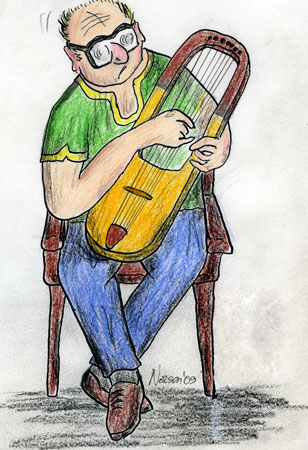
\includegraphics[width=4cm]{main/Logo_Livre.jpg}}%
				\hspace{1cm}%
			\end{center}%
		\end{figure}%
	}\newpage\thispagestyle{empty}
	{\bfseries\fontsize{14}{16}\selectfont{}ÉDITIONS}\par

	{\fontsize{14}{16}\selectfont{}La forêt du grand Méchant Loup\\
														Adresse Non disponible\\
														666 Avenue du Libre }\par
	\vspace{\stretch{3}}
	{\fontsize{12}{14}\selectfont{}Ce livre et l'illustration en couverture sont publiés sous la licence libre\\\textbf{Creative Commons-BY-SA} :\\\url{http://creativecommons.org/licenses/by-sa/2.0/fr}\par}
}
{\setlength{\parskip}{1.5\baselineskip}
	\textbf{BY : Paternité.} Vous devez citer le nom de l'auteur original.\par
	\textbf{SA : Partage des Conditions Initiales à l'Identique.} Si vous modifiez, transformez ou adaptez cette création, vous n'avez le droit de distribuer la création qui en résulte que sous un contrat identique à celui-ci.\\
	En outre, à chaque réutilisation ou distribution, vous devez faire apparaître clairement aux autres les conditions contractuelles de mise à disposition de cette création. Chacune de ces conditions peut être levée si vous obtenez l'autorisation du titulaire des droits.\par
}
\vspace{\stretch{2}}
{\centering\setlength{\parskip}{2\baselineskip}
	In Libro Veritas, \anneedepot{}, ISBN : \isbn\par
	Dépôt légal : \datedepot\par
}
\vspace{\stretch{4}}
\sommaire
\TitreIntro{Préface}

%\newline

% J'ai enlevé la lettrine car ca faisait pas beau. Si vous trouvez comment améliorer ca à vous de le changer!
%\begin{floatingfigure}[]{5mm}
%
\includegraphics[height=10mm]{intro/preface/img/lettrine-i.jpg}
%\end{floatingfigure}

Il arrive quoi dans un sous-sol démoralisant, anémiant et sale, lorsque des gens jusque-là prostrés, cloîtrés et gommés des registres, se mettent à vivre toute une gamme de sentiments humains, partant de vieilles blessures cachées bien creux qui s’ouvrent, passant par des décennies de non-dit, de colère refoulée et d’ambitions détruites, finissant dans les larmes, le sourire et le bonheur ? Il arrive quoi si ces gens sont âgés, désabusés, démunis et totalement dépendants de la bienveillance sans borne d’un fils persécuté qui, à 43 ans, est encore puceau et déteste jouer du trombone ? Que se passe-t-il quand ces gens se cachent d’un système qui traque et enferme les vieux dont certains se retrouvent intubés dans un projet de production hormonale ? Il arrive une histoire sordide où les méchants sont vraiment affreux, une histoire rocambolesque où les bons sont hauts en couleur, une histoire d’amour pleine de chaudes émotions sous fond de musique allemande, Wie einst Lili Marleen, une histoire de commando dont le colonel est l’arrière-petit-fils de l’inventeur du Pétépano et la générale, une joueuse de violoncelle..

\begin{floatingfigure}[r]{40mm}
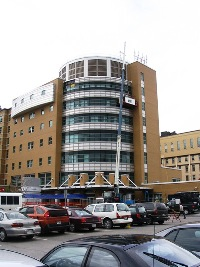
\includegraphics[height=60mm]{intro/preface/img/hopital.jpg}
\end{floatingfigure}

Pourtant, l’idée de départ était bien différente. Elle était sensée répondre à mes craintes quant aux années à venir. Elle se basait sur un fait vécu, une anecdote déplaisante que j’avais à peine arrangée et qui avait pour cadre une salle d’urgence québécoise durant l’été 2008.La dame a son expression des grands jours, celle où c’est écrit «j’ai pas le temps de niaiser».

- Maman, ils m’ont dit de venir te chercher, qu’ils ne pouvaient plus te garder, qu’il me fallait te ramener à la maison.

Puis, pour elle-même, elle ajoute :

- Qu’il fallait qu’à 57 ans, j’apprenne à être ton «aidant naturel».

La vieillarde décoiffée et édentée lève un peu la tête de sa civière. De ses yeux creux, elle regarde cette femme en larmes qui la dévisage de si près. Elle ne comprend pas et se retourne vers le mur. Derrière elle, devant elle, d’autres civières. Des cancers, des poumons, des boyaux, des os, des enflures, des cirrhoses. Ça sent le cabinet d’aisance achalandé. Il fait chaud à vomir. Ça geint, ça craint, ça ne veut pas être seul, ça veut savoir. Sans arrêt, des hommes et des femmes en uniforme d’hôpital passent, toujours à la course, toujours pour d’autres, toujours avec d’autres priorités, toujours sans les regarder. Des ambulanciers vont et viennent des dossiers en main. Des bonhommes promènent leur verre de styromousse plein de café de machine, d’autres essaient de regarder une télé pas de son qu’on a boulonnée trop haut pour être vue sans torticolis, d’autres se sont ramassé le Journal de Québec et, après les petites annonces, en sont rendus à lire les avis de décès non sans quelque espoir de pouvoir bientôt y figurer. Des portes claquent, des chaises grincent, des chariots couinent.

- Maman, aide-moi. Faut que tu t’asseyes ici; je t’ai amené une chaise roulante.

La vieille dame ne bouge pas.

- S.V.P., maman.

Rien ne se passe jusqu’à ce qu’une préposée expérimentée ne vienne s’en mêler.

- Madame Dubé, fait-elle à voix haute de son timbre pointu, Madame Dubé !

Rien !

- Madaaaam ! Madaaaam !

Toujours rien !

- Vous voyez bien qu’elle n’est pas capable, dit la dame à la préposée.

- Vous êtes sa fille ?

- Oui. Ils m’ont dit de venir la chercher.

- Madaaaam ! Madaaaam !

Vingt minutes passent pendant lesquelles deux ambulances viennent déverser les deux victimes d’un gros accident sur les lits déjà trop pleins de l’Urgence. Faut voir les proches qui pleurent, qui se consolent, qui veulent savoir, qui ne comprennent pas. Qui va-t-on tasser pour faire place à ces nouveaux qui saignent, qui ont plein de trous par où la vie est en train de filer ?

La préposée est revenue avec une infirmière.

- Vous êtes sa fille ? demande cette dernière.

- Oui. Ils m’ont dit de venir la chercher.

- Pourquoi qu’elle est ici ?

- Alzheimer, de l’eau aux poumons, de l’arythmie et elle va avoir 87 ans.

- Pelaille ! P’is ils vous ont dit de venir la chercher ?

- Oui, ils peuvent pas s’en occuper.

La préposée s’est penchée sur la vieille.

- Madame Dubé, Madaaaam !

- Attends un peu, je vais vérifier de quoi, lui dit l’infirmière, stéthoscope sur les oreilles.

La dame aimerait pleurer, mais elle se retient du mieux qu’elle le peut.

- Je reviens, lui dit l’infirmière.

Cette fois, il faut moins de deux minutes. La professionnelle réapparaît avec un médecin cerné comme s’il n’avait pas dormi de la semaine. Il se penche, regarde, taponne, écoute, stéthoscopise.

- Vous êtes sa fille ?

- Oui. Je suis Sylvie Dubé.

- Il faut la rentrer aux soins intensifs. Demain, on verra. Mais à soir, on la monte.

- Oui, mais ils m’ont dit de venir la chercher …

- Madame, faut la monter tout de suite.

Une heure plus tard, la dame est assise dans l’auto de son conjoint qui vient d’arriver, les essuie-glaces en folie. Le visage bouleversé, peut-être apeuré, elle lui demande :

- Que c’est que ça va être, quand ça va être notre tour ?

Cette dernière réplique m’a servi de titre de travail pendant quelques semaines, le temps d’imaginer une histoire avec plein de vieux dans des lits, des vieux très malheureux, tout entubés, mal nettoyés, traités comme des lépreux. Et des préposés absolument pas respectueux, très détestables, des têtes à attendre la paie, à être malhonnêtes et profiteurs. Sans parler de familles absentes, heureuses de s’être débarrassées de leurs misérables fardeaux. Une histoire qui se termine en 2034, 50 ans après 1984, année choisie par George Orwell pour présenter une société de machines où la norme est de ne pas avoir de cœur.

\begin{floatingfigure}[l]{15mm}
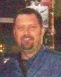
\includegraphics[height=15mm]{intro/preface/img/simon1.jpg}
\end{floatingfigure}

Malgré ce cadre épouvantable, mon histoire est très rapidement devenue humaine et son ton, humoristique. D’entrée de jeu, elle a versé dans un rapport mère-fils compliqué, un problème d’estime de soi majeur, des relations interpersonnelles difficiles, des histoires de haine intergénérationnelle, sans parler d’une difficile cohabitation avec un chien très laid et très méchant. J’ai vite compris qu’il me fallait demander conseil au copain Simon Atkins, un psy de la grande région de Toronto - là-bas, ils disent «psychotherapist» - qui, effectivement, m’a fait l’amitié de me redresser un personnage ou deux.

Voici d’ailleurs ce qu’il raconte sur cet exercice.

«De ma banquette, j’écoute, malgré le brouhaha du resto, la narration d’une histoire qui arrive à sa conclusion, un chassé-croisé harmonieux de mots en train de se tisser en un dernier accord. Je perçois très bien la couleur, l’émotion, l’obscurité, puis la lumière qui précède l’aurore annonciatrice. En même temps, je me sens un peu triste de ne pas entendre la langue de Ducharme, de Vigneault, de Desjardins. Mais, connaissant Nelson depuis des lustres, j’ai quand même droit au récit avant publication.

Ce gars est un conteur doué, un conteur généreux, qui nous convie, au propre et au figuré, à le retrouver dans son jeu créatif, dans un plaisir enrichissant où nous faisons nôtres, les luttes auxquelles doivent se livrer les personnages. Le joueur de lyre nous rappelle ce qui est vraiment important dans nos vies, dans nos relations et dans notre communauté. Je suis convaincu que de nombreux lecteurs et lectrices sentiront de façon particulière les blessures, la solitude et même le désespoir qui se dégagent au fil des chapitres.

Quel est le prix à payer pour avoir porté, toute notre vie, de vieilles blessures qui nous ont empoisonné le quotidien et qui nous ont empêché de communiquer comme il l’aurait fallu avec notre entourage ? Qui a-t-il de bon à vieillir, si nous devons nous retrouver en marge de la vie active, celle des jeunes et des puissants ? Quel est le rôle de la culture dans la définition de qui nous sommes et dans la nature des réflexions ou des rêves que nous aimerions partager avec nos proches ? Autant d’interrogations avec lesquelles ce roman nous interpelle en pointant sur notre passé pour mieux comprendre notre parcours actuel.

L’auteur nous a accrochés à son histoire en la publiant par tranches, chaque semaine, sur la Cyberpresse où il nous a invités à réagir. Cela lui a permis d’être en situation de mieux la dessiner. Ce faisant, il nous a rassemblés autour d’une nouvelle forme de récit, une collaboration en ligne qui remet en question, donc renforce, le fil conducteur du roman. À l’instar de Timothée de Milet, ce musicien de la Grèce antique qui aurait rajouté quelques cordes à la lyre de son époque, Nelson nous entraîne à ajouter des notes à sa trame romanesque, des notes accordées en notre for intérieur qui viennent former un chœur.

Si l’allégorie utilisée peut nous faire réfléchir sur l’état de notre quotidien familial, elle peut surtout nous inspirer le courage de vouloir guérir nos vieilles blessures, la sagesse d’éviter les pièges dans lesquels nous sommes déjà tombés et le goût d’aller offrir de la tendresse aux gens autour de nous, quelque soit notre âge.

Je vous souhaite d’apprécier la musicalité des mots qui s’échappent de la lyre de Nelson.

Alliston, janvier 2009 »

Ce chœur dont parle Simon, c’est celui qui s’est spontanément formé quand, le 16 septembre 2008, j’ai commencé à mettre Le joueur de lyre en ligne, un chapitre par semaine. Pour intégrer cette douce activité de scribouillage dans ma semaine d’écriture professionnelle (j’ai à publier des articles technos tous les jours), les autorités de la Cyberpresse (qu’au passage, je remercie chaleureusement) acceptèrent qu’elle devienne ma prestation du vendredi. Si j’arrivais à divertir mes lecteurs tout en respectant leur intelligence, peut-être me fourniraient-ils la rétroaction nécessaire à la fabrication de mon histoire. Ce qui fut fait pendant quatre mois, jusqu’au 16 janvier 2009 (il y eut relâche le 2 janvier), période au cours de laquelle 19 chapitres furent écrits, publiés, commentés et bonifiés. Des personnages durent être ajoutés, des personnages secondaires empruntant souvent des pseudonymes utilisés par des usagers de la Cyberpresse. Avec leur assentiment, va s’en dire.

Au début, les suggestions furent nombreuses quant à la suite à apporter à cette sombre histoire de centres régionaux gériatriques, de vieillards traqués par la police, de grabataires nourris au manger mou, c’est-à-dire au Nutrisuz. Puis, ce fut l’accalmie. Comme si on préférait me regarder aller avec ma trame romanesque. Comme si on s’accommodait de mes personnages caricaturaux qui vivaient de dures péripéties d’humain, mais qui luttaient pour s’en sortir, ce qui laissait présager d’une fin heureuse et acceptable dans toutes les bibliothèques familiales. Certaines et certains continuèrent à m’éplucher, à me dénicher des erreurs de fait, à m’épingler sur des incongruités, sans oublier l’inévitable cortège de fautes d’orthographe. Elles, ils, le firent jamais méchamment, toujours avec humour. Un vrai plaisir.

\begin{floatingfigure}[r]{30mm}
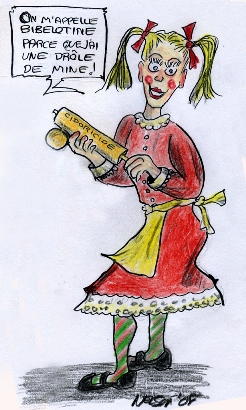
\includegraphics[height=60mm]{intro/preface/img/personnage-bibelotine.jpg}
\end{floatingfigure}

Évidemment, je suis journaliste pigiste, ce qui est un avantage réel par rapport au romancier de métier, un créateur isolé qui, comme le veut le cliché, applique avec rigueur la trame qu’il a imaginée et qui, durant le processus de création, limite l’interaction au minimum vital. C’est qu’avec le temps, le pigiste n’a plus d’ego; les éditeurs, rédacteurs en chef et autres chefs de pupitre le lui ont bouffé en totalité. Ainsi, que des lecteurs lui mettent publiquement sous le nez une «hénaurme» faute d’orthographe, une phrase boiteuse, une imprécision mortelle, une invraisemblance inopportune, ça ne l’affecte pas. Bien au contraire. Il s’en montre ravi, convaincu que son produit vient d’être amélioré. Qu’une lectrice ou un lecteur lui change un recoin d’histoire en y ajoutant une perspective amusante, il la fait sienne et se dépêche d’en donner le crédit à la si gentille personne.

Dans les pages qui suivent ce roman, vous trouverez mon analyse du processus encouru, une démarche que l’on dit de type «Web 2.0». Vous rencontrerez le chœur dont parle Simon, vous jugerez du sérieux de son apport, de sa générosité et de sa gentillesse. Vous saurez pourquoi, dans Le joueur de lyre, il ya des personnages qui se nomment Bea Bellow, Vlado Markovsky, Anton Suzkinne, Thierry-Ian Dennis-Dubeau, Louise Lavoie, Tropecolo, Philippe Flipper Dauphin, les Papyblues et autres docteurs Bellavance. Surtout, vous comprendrez mon envie de recommencer la même expérience avec une nouvelle histoire dès que ce sera possible.

En parallèle avec ce magnifique chœur, j’ai soumis mes interrogations, mes angoisses, mes incompréhensions, à une belle soliste, ma blonde Darisse, une personne d’une sensibilité prodigieuse qui a su me saupoudrer l’histoire de considérations humaines. Je lui dois notamment les réactions complexes du personnage de Marie-Odile Tremblay. Plus globalement, elle a, semaine après semaine, écouté mon récit du chapitre devant être mis en ligne et m’a régulièrement aidé à le solidifier. 

%\begin{floatingfigure}[l]{15mm}
%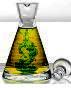
\includegraphics[height=10mm]{intro/preface/img/druide1.jpg}
%\end{floatingfigure}

En terminant, un remerciement à André d’Orsonnens, PDG de Druide informatique, qui m’a gracieusement fourni un exemplaire d’Antidote, le coffret d’outils linguistiques bien connu. Dans le cas d’un pigiste devant mettre en ligne, tous les vendredis matin, un texte de quelque 7 000 mots se voulant un nouveau chapitre du Joueur de lyre, ce logiciel montréalais m’a fait gagner beaucoup de temps.

Voilà ! Bienvenu dans mon histoire et bonne lecture ! On se retrouve plus tard, pour la partie analyse.

Nelson Dumais, janvier 2009


% LES "INCLUDES" SUIVANTS DONT DÉSACTIVÉS CAR JE N'EN AI PAS ENCORE DE BESOIN POUR LA MARIRIOU. JE LES LAISSE JUSTE AU CAS OU! 
%% ATTENTION - LIRE - CETTE PAGE PROVIENT DU DOCUMENT SOURCE DE DIDIER ROCHE ET N'EST PAS UTILISEE PRESENTEMENT POUR LA MARIRIOU. 
% JE L'AI LAISSEE ICI JUSTE EN CAS DE FUTURE AJOUTS ET/OU MODIFICATIONS SI NECESSAIRE.

\TitreIntro{Notre public}
Ce livre s'adresse tout particulièrement aux utilisateurs de Windows désireux de passer sous GNU/Linux. De plus, il peut aussi présenter la distribution Ubuntu à des utilisateurs d'autres distributions Linux, et également aux possesseurs de systèmes Mac Os X. De nombreuses captures d'écran jalonnent ce livre pour que, je l'espère, vous ne soyez jamais perdu.\par
Ce livre ne fera pas de vous un maître incontesté de GNU/Linux\NotePage{Bien que lorsque vous arriverez à l'avant-dernier chapitre, vous commencerez à en maîtriser les ficelles !}, mais vous guidera dans vos premiers pas sous Ubuntu pour que vous sachiez l'installer, ajouter de nouveaux logiciels et jeux, et l'utiliser quotidiennement. De plus, il constitue une bonne introduction à une compréhension plus avancée du système d'exploitation et vous donnera les clefs pour aller plus loin, si vous le désirez\ldots{}\par

%% ATTENTION - LIRE - CETTE PAGE PROVIENT DU DOCUMENT SOURCE DE DIDIER ROCHE ET N'EST PAS UTILISEE PRESENTEMENT POUR LA MARIRIOU. 
% JE L'AI LAISSEE ICI JUSTE EN CAS DE FUTURE AJOUTS ET/OU MODIFICATIONS SI NECESSAIRE.

\TitreIntro{Le plan de cet ouvrage}
Ce livre se veut comme une progression pas à pas dans la découverte de votre nouveau système d'exploitation ; chaque chapitre marque une étape importante de ce déroulement. Je conseille donc à tout nouvel apprenti de lire ce livre dans l'ordre, sans faire de grandes coupes franches afin de comprendre sans trop d'efforts les étapes suivantes.\par
\begin{DescriptionChapitres}
\item [Chapitre 1] Ce chapitre comprend une courte introduction au Logiciel Libre et, en particulier à GNU/Linux, en insistant sur la philosophie et les différences avec le logiciel propriétaire. Vous y trouverez également les réponses à quelques questions d'ordre général.
\item [Chapitre 2] On y découvre comment obtenir Ubuntu, l'essayer sans risquer de perdre des données et enfin, se lancer dans une séance d'installation.
\item [Chapitre 3] Le chapitre 3 explique les notions de base à connaître lorsque l'on «~plonge~» dans GNU/Linux ! Il vous guidera aussi dans la découverte de votre nouvel environnement de travail.
\item [Chapitre 4] Vous trouverez dans ce chapitre une explication sur l'installation d'un réseau (et de l'Internet) sur votre nouveau système d'exploitation. Vous serez également initié à la bonne manière de procéder à l'installation de logiciels et de jeux à partir des outils mis en place par Ubuntu.
\item [Chapitre 5] Il présente les derniers points à effectuer pour rendre votre système utilisable quotidiennement, avec, par exemple, le téléchargement des codecs vidéos, la liaison de Firefox avec des composants tels que Flash et Java\ldots{}
\item [Chapitre 6] Voici sûrement le chapitre qui vous intéressera le plus : il décrit les trucs et astuces qui permettent de gagner du temps et d'utiliser plus intelligemment son environnement de travail. Vous y trouverez également quelques conseils sur l'utilisation de Firefox.
\item [Chapitre 7] Le chapitre 7 traite des derniers points matériels qui peuvent poser problème comme la configuration de l'imprimante. Il vous guide également à l'aide d'un exemple dans l'utilisation d'un scanner, du bureau 3D et d'une configuration de démarrage.
\item [Chapitre 8] Vous y trouverez une liste de logiciels classés par catégorie permettant rapidement de repérer et choisir un logiciel à installer pour tel ou tel type d'utilisation.
\item [Chapitre 9] Dans le chapitre 9, vous découvrirez un nombre impressionnant de jeux disponibles sous GNU/Linux. Ceux-ci, classés par genre, contiennent les instructions complètes d'installation.
\item [Chapitre 10] Le chapitre 10 est un aparté qui peut vous emmener plus loin dans la connaissance et la compréhension de votre système d'exploitation. Bonne nouvelle, celui-ci est optionnel !
\item [Chapitre 11] Conclusion de cet ouvrage, ce chapitre vous permettra de savoir où chercher de l'aide, des informations et comment s'investir dans le monde du Libre.
%il présentera notamment des notions telles que «~Pourquoi le libre~» et vous amènera très certainement à voir les enjeux présents et la culture libre sous un angle différent.
\item [Glossaire] Le glossaire vous permettra d'accéder rapidement à la définition de certains termes réservés au monde de l'informatique.
\item [Index] Un index, très pratique, vous renverra, à l'aide d'une recherche par catégorie et mots-clefs, aux pages du livre correspondantes.
\item [Table des matières] Une table des matières complète, recensant toutes les sections de cet ouvrage, clos ce livre.
\end{DescriptionChapitres}

%% ATTENTION - LIRE - CETTE PAGE PROVIENT DU DOCUMENT SOURCE DE DIDIER ROCHE ET N'EST PAS UTILISEE PRESENTEMENT POUR LA MARIRIOU. 
% JE L'AI LAISSEE ICI JUSTE EN CAS DE FUTURE AJOUTS ET/OU MODIFICATIONS SI NECESSAIRE.

\TitreIntro{Conventions utilisées dans ce livre}
\label{RefExemple}
Pour permettre une lecture et un repérage plus simple de ce livre, voici les conventions que l'on s'est fixées :\par
Un renvoi vers une autre partie du livre est indiqué de la sorte : cf. page \pageref{RefExemple}.\par
Les notes de bas de page sont représentées ainsi\NotePage{Je ne sais pas si vous avez remarqué, mais la référence précédente était une référence auto-récursive ;)}.\par
La navigation entre un menu et un sous-menu est séparée par cette flèche \FlecheDroite très esthétique !\par
Des chemins vers des fichiers et des dossiers sont présentés de cette manière : \Chemin{vers/l/infini/et/au/delà}.\par
Une touche du clavier est mise en évidence comme la touche \Touche{Entrée}. Un signe + est ajouté si vous devez presser simultanément plusieurs touches.\par
Un élément décrit dans le glossaire$^*$ bénéficie également d'une mise en évidence particulière.\par
Les commandes à entrer dans un terminal sont mises en valeur de cette manière : \Commande{Une ligne de commande}. Elles sont -- le plus souvent -- à saisir sur une seule ligne, la mise en page d'un livre ne permettant pas, la plupart du temps, de l'écrire ainsi.\par
Une note plus longue -- et plus importante -- est indiquée de la sorte : \begin{nota}Cette note devrait normalement apporter des précisions supplémentaires au sujet précédent. Cependant, ces informations ne sont pas non plus capitales.\end{nota}\par
Les notes plus importantes, quant à elles, sont représentées comme ceci : \begin{attention}Ceci est une note importante, elle essaie d'attirer votre attention sur un point précis à ne pas négliger afin que la suite des opérations indiquées dans le livre se déroule sans heurts.\end{attention}\par
Les lignes de code représentent la sortie du terminal. Cette présentation est également utilisée lorsqu'un grand nombre d'éléments sont à entrer dans un fichier : \Code{\# Ceci est un commentaire dans un fichier de configuration\\
\# Le plus souvent, ce dernier est présent sur plusieurs lignes}\par
Quelques citations jalonnent ce livre et sont représentées de la sorte :\par
\begin{citationlongue}{Pythagore a dit}
Les amis sont des compagnons de voyage, qui nous aident à avancer sur le chemin d'une vie plus heureuse.
\end{citationlongue}\par
Ce livre existe également dans un format électronique où les adresses internet comme celle de framabook -- \url{http://www.framabook.org} -- sont des hyperliens, et les liens internes comme les notes de bas de page sont également actifs.\par
\vspace{\stretch{1}}
Je tiens enfin à rappeler que les adresses Internet sont malheureusement par nature, appelées à varier : un lien, valide lors de l'écriture de ce livre, peut donc devenir invalide.
\vspace{\stretch{10}}

%% ATTENTION - LIRE - CETTE PAGE PROVIENT DU DOCUMENT SOURCE DE DIDIER ROCHE ET N'EST PAS UTILISEE PRESENTEMENT POUR LA MARIRIOU. 
% JE L'AI LAISSEE ICI JUSTE EN CAS DE FUTURE AJOUTS ET/OU MODIFICATIONS SI NECESSAIRE.

\TitreIntro{Remerciements}
\begin{Remerciements}
Je tiens à remercier tout d'abord les développeurs de logiciels libres et leurs contributeurs, en particulier ceux de la Fondation Ubuntu, pour leur sens de l'intérêt général, du partage, de l'entraide et de l'innovation. Merci également à \Personne{Mark}{Shuttleworth} pour son dynamisme et sa communication sur les objectifs de sa distribution.\par
Je n'oublie pas non plus mes parents qui m'ont permis d'accéder à l'outil informatique dès mon plus jeune âge. Je tiens également à saluer \Personne{Vanessa et Dimitri}{Perrin} pour leur soutien et pour avoir rendu mon séjour en Irlande agréable.\par
Cette tâche a été effectuée à partir de l'énorme travail d'\Personne{Anthony}{Carré}\NotePage{\url{http://yeknan.free.fr}}, initialement adapté au format imprimable par jokx\NotePage{\url{http://wenux.net}}, ce qui m'a plus que motivé à la rédaction de ce document. J'aimerais aussi inclure dans les remerciements les trois co-auteurs \Personne{Julien}{Rottenberg}, \Personne{Guillaume}{Ludwig} et \Personne{Joseph}{Massot}. Leur livre n'a malheureusement jamais pu sortir. Les parties de l'installation de l'imprimante et du scanner sont (quasi) intégralement basées sur leur travail, ainsi que quelques ajouts dans la description des menus.\par
Cette documentation est également «~librement~» inspirée de quelques billets du blog de \Personne{David}{Szerman}\NotePage{\url{http://www.szdavid.com}}, de \Personne{Jean-Baptiste}{Hétier}\NotePage{\url{http://www.think-underground.com}}, de Asher\NotePage{\url{http://asher256.tuxfamily.org}} -- par son travail sur son dépôt -- de  \Personne{Grégory}{Gutierez}\NotePage{\url{http://petitlinux.greguti.com}}, sans oublier le wiki de notre chère communauté francophone\NotePage{\url{http://doc.ubuntu-fr.org}} et sa mailing-list toujours aussi accueillante. L'excellent site \url{http://www.whylinuxisbetter.net} a également été une source d'inspiration importante, merci à  \Personne{Manu}{Cornet}, son créateur.\par
Ce livre réalisé en \LaTeX{} n'aurait jamais été possible sans l'excellent guide «~Tout ce que vous avez voulu toujours savoir sur \LaTeX{} sans jamais oser le demander~» de \Personne{Vincent}{Lozano}, Framabook dont la sortie est imminente. Surveillez \url{http://www.framabook.org} !\par
Un grand merci également à toutes les personnes qui ont apporté leur pierre à l'édifice par le biais du forum, notamment \Personne{Raphaël}{Bourven} pour son énorme travail de relecture\NotePage{Et il a même re-signé pour les nouvelles versions, le bougre !} et les nombreuses corrections apportées par la communauté d'Ubuntu-fr dont \Personne{Fabrice}{Braillon}, \Personne{Franck}{Chadel}, \Personne{Quentin}{Bricard} et \Personne{Claude}{Crozet}, ainsi que par le contributeur très productif qui sait se lancer dans un sprint final éhonté\NotePage{Il ne sait que trop bien ce que signifie «~On boucle demain midi !~» ;-)}, à de multiples reprises : \Personne{Bruno}{Le Clainche}.\par
Cette version a également bénéficié du groupe de lecture de Framabook par les participations actives de \Personne{Barbara}{Bourdelles}, \Personne{Raymond}{Rochedieu}, \Personne{Antoine}{Blanche} et Metta Om.\par
Enfin, je témoigne ma gratitude à \Personne{Alexis}{Kauffmann}\NotePage{\url{http://framablog.org}}, fondateur de Framasoft\NotePage{\url{http://www.framasoft.net}} pour avoir cru qu'il était possible de transformer ma documentation en un livre, qui, je l'espère, vous plaira, ainsi qu'à \Personne{Mathieu}{Pasquini}\NotePage{\url{http://www.inlibroveritas.net}}, mon éditeur, pour son soutien même dans les moments les plus difficiles.\par
Ce livre essaie de respecter au maximum les règles de la typographie française, même si\NotePage{Oui, je fais du préventif pour éviter toute critique !}, je suis tout à fait conscient que, comme je vous le présenterai en \ref{refMajAccent}, la première lettre de l'introduction du chapitre \ref{RefDebutChap7} page \pageref{RefDebutChap7} devrait être accentuée. Il s'agit toutefois d'un problème auquel j'ai fait face avec \LaTeX{} sans, malheureusement, arriver à le résoudre à cet instant.\par
Pour toute remarque ou suggestion constructive concernant ce livre, vous pouvez ouvrir un sujet dans la section «~Framabook.org~» de Framagora\NotePage{Forum de Framasoft} à l'adresse suivante : \url{http://forum.framasoft.org}.\par
\end{Remerciements}

%% ATTENTION - LIRE - CETTE PAGE PROVIENT DU DOCUMENT SOURCE DE DIDIER ROCHE ET N'EST PAS UTILISEE PRESENTEMENT POUR LA MARIRIOU. 
% JE L'AI LAISSEE ICI JUSTE EN CAS DE FUTURE AJOUTS ET/OU MODIFICATIONS SI NECESSAIRE.

\TitreIntro{À propos de l'auteur}
En 1990, \Personne{Didier}{Roche} se découvre très jeune une grande passion pour l'informatique. Il s'adonne très vite, avec un réel intérêt, à la programmation et en apprend de très nombreux langages dans ses années de collège-lycée. À partir de 2002, il effectue des études supérieures d'ingénieur généraliste à l'ECAM\NotePage{École Catholique d'Arts et Métiers, Lyon}. Profitant de ces années pour entrer dans une association humanitaire dont l'objectif est d'amener des ordinateurs dans les écoles et universités d'Afrique et de former sur place étudiants et professeurs à l'utilisation de l'outil informatique -- association Afric'Edu\NotePage{Association pour la Formation de Réseaux Internet Commis à l'Education et au Développement des Universités} basée à Lyon -- ceci le conduira notamment au Togo pendant le mois de juillet 2006, donnant accès à l'informatique à plus de 2000 élèves et professeurs. Actuellement, il travaille dans une grande société française d'édition logicielle, leader dans les solutions de PLM\NotePage{Product Lifecycle Management : gestion de cycle de vie des produits} en tant qu'ingénieur informaticien de production.\par
Concernant sa pratique de Linux, son premier essai de migration date de 1996 avec une Red Hat qui s'avèrera être un échec puisqu'il n'y resta pas très longtemps. Sa seconde migration, cette fois réussie à l'aide d'une Mandrake\NotePage{Nommée aujourd'hui Mandriva pour une sombre histoire de licence avec ... le magicien du même nom !} 7, fit de lui un Linuxien convaincu ! En 2004, il découvrit la distribution Ubuntu\NotePage{Alors qu'elle n'avait pas encore de nom définitif !} qui allait devenir son système d'exploitation principal. Il se découvre alors une réelle passion pour le Logiciel Libre et y consacre la plupart de son temps «~libre~» aussi en tant qu'administrateur de la partie documentation du site Ubuntu-fr et membre du comité de pilotage des Framabooks.\par
Didier Roche a choisi de reverser 20 \% de ses droits d'auteur également répartis entre les associations Ubuntu-fr et Framasoft.org afin de les soutenir et de les remercier pour leurs extraordinaires travaux.\par

\mainmatter % Corps du livre
\chapitre{Un sous-sol à Nazareth, le lundi 18 juillet 2033} {D'aucuns diraient}{ qu’il fait chaud pour mourir, que c’est sale partout, que ça sent le vieux, que la bonne femme est due pour un bain et le bonhomme, pour un récurage à la brosse. Mais à quoi cela servirait-il de le penser. «D’aucuns» n’existent pas, personne, sauf le fils, ne vient ici. Personne ! Jamais ! Et il ne peut en être autrement; c’est la nature même du châtiment. Personne ne peut imaginer venir ici parce que personne ne peut imaginer qu’il y habite des gens, enfin des vieux qui ne sourient jamais et qui se parlent que très rarement.}

À 82 ans, Marie Rioux est devenue «sec comme un balai» ; pas une once de graisse ne l’enrobe et son dos n’a pas encore commencé à voûter. «Rien à gruger su’ l’os», aurait dit son oncle Robert, autrefois plombier à Québec. Vêtue d’un vieux Levys foncé, ceux qu’elle préférait, et d’un antique coton ouaté commémorant la victoire de Barack Obama aux présidentielles américaines de 2008, elle s’occupe à faire luire le bois de son violoncelle. Autant le jeans que le chandail sont délavés, tout comme ses cheveux remontés en toque qui sont devenus blanc jaune. Ses pieds sont chaussés de bas de laine troués achetés, naguère, dans un surplus de l’armée. Ses mains sont longues, criblées de taches, bosselées par l’arthrite et ses ongles ne sont presque plus entretenus. D’ailleurs, pourquoi le ferait-elle? Pour qui ?

Son compagnon, cet être édenté, mal rasé, calé dans son lazy boy, les lèvres et la langue faisant «bleblebleblebleblebleble» à chaque respiration, se nomme Romain Tardif dit «le gelé». Il échappe la télécommande qui, sans bruit, choit sur le tapis moucheté de gris et de beige, un tissu fatigué dont la vocation est d’absorber poussières et petits détritus sur tous les planchers du sous-sol. L’homme se réveille en sursaut, convaincu d’avoir commis un impair majeur.

Assise juste à côté dans l’autre misérable fauteuil, la vieillarde le fixe de ses yeux superbes, des charbons qui n’ont pas vieilli, mais dont le potentiel de causticité, d’implacabilité et même de venimosité est demeuré aussi redoutable qu’il y a 53 ans. À ses pieds, la tête sur ses courtes pattes crochues, Gazou, un animal hargneux, mi-rat, mi-loulou obèse - ceux qui font “tic-tic-tic-tic” en marchant sur le prélart - une sale bête de chien jaune à poil ras et au nez brun avec, en tout temps, un croc saillant sur le museau, regarde avec haine la télécommande qui vient de le tirer de son sommeil. Sans rien dire, Marie reprend sa méticuleuse opération.

«Qu’elle était belle et séduisante», se remémore l’homme en s’étirant légèrement la jambe gauche, celle de son nerf sciatique. Puis, comme s’il eut voulu exaspérer davantage Marie et sa bête, il baille à s’arracher le maxillaire tout en son et lumière.

Étrangement, il a été épargné par la calvitie et sa tignasse blanche tout ébouriffée se termine en queue de cheval, laquelle date, selon toute apparence, du temps de sa moustache à la Frank Zappa, Sonny Bono ou Hulk Hogan. Le bonhomme est habillé d’un improbable short Nike, le modèle rouge à bandes noires sur les hanches, un short suspect taché d’on ne sait trop quoi, d’une camisole devenue jaune qui cache à peine ses chairs amollies, d’une paire de chaussettes bien étirées vers les mollets, des chaussettes ahurissantes à motifs de Schtroumpf, et de sandales avec semelles en retaille de pneu.

\begin{floatingfigure}[l]{40mm}
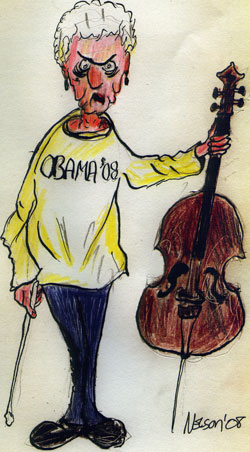
\includegraphics[height=60mm]{corps/chapitre1/img/maririou062.jpg}
\end{floatingfigure}

- Gajoo, rechte à côté de Maman, chinon, tu vas payer pour. Ta-tchu compris ?

Le chien jaune se replonge le mufle dans les pattes. De son œil hypocrite, il a vu que «Maman» ne blaguait pas et il se méfie de son archet.

Dans ce modeste logement de Nazareth, quartier s’étirant de Sacré-Cœur à la rivière Rimouski, on ne retrouve aucune photo sur les rares espaces que le rayonnage irrégulier de livres n’a pas volé aux murs. Ni de ces deux vieux assis la mâchoire pendante devant la télé, une antique HD aux couleurs déphasées, ni d’enfants potelés laissant paraître une dent au travers de leur sourire habituellement qualifié d’angélique, ni de scènes du «bon vieux temps d’avant le sida» alors que tout était si «désormais» facile, si «définitivement» cool, ni de fumeurs de cigarettes, oncles ou cousines depuis longtemps disparus, croqués en noir et blanc dans leurs vies de misère à la merci de la damnation éternelle, ni de guitaristes rock drapés dans le très pop Star-Spangled Banner. On ne retrouve aucune photo, pas plus qu’on ne remarque de reproductions de Toulouse-Lautrec, de nature morte peinte par la tante Hermance, cette vieille chipie de chez les Tardif, d’horloge Molson Export volée dans un hôtel de saint en arrière, d’écran plasma sans fil au récepteur défectueux, de feuilles de «pot» séchées et vernies, de poster du Che, de Dalida ou de Bob Dylan.

Plutôt, ici et là, une partition musicale imprimée sur du papier jauni, un calendrier de 1980 émis par le garage Rhéo Lavoie Auto Body enr. où une fillette sourit à côté de son chien Collie dans une Chevy rouge décapotable de 1955, un document laminé signifiant son congé de l’Hôpital St-Joseph de Rimouski à une patiente dénommée Marie Rioux et une lettre ravagée par le temps où apparaît clairement la signature inesthétique d’une enflure locale, régionale et nationale appelée Sylvain Turcotte.

Mais l’attention est surtout portée vers une fenêtre panoramique violemment éclairée par le fleuve, son ciel au bleu si particulier, ses îles, la Canuel vers l’ouest et la Saint-Barnabé juste en face, cette dernière se substituant à la ligne d’horizon où on devrait deviner la ligne très fine de la Côte-Nord, contrée aux si pénibles souvenirs. En s’étirant le cou vers la droite, on peut quasiment apercevoir Pointe-au-Père tel un mauvais rendu de Google Map. Un store vénitien à lames en bois franc poussiéreuses a été tiré vers le haut afin que rien de ce décor ne soit perdu. Comme s’il fallait vraiment expier. Et, la cruelle lumière de cet après-midi d’été met bien en relief la grasse saleté encollée aux vitres et, surtout, les poussières de toutes tailles et de toutes «origines» qui flottent dans l’air surchauffé de l’appartement. Le thermostat électronique indique en effet 29 degrés Celsius et toute entrée d’air semble bloquée. À dessein !

À la gauche de cette fenêtre, un exerciseur de marche au tapis usé à la corde obstrue une partie du passage menant à la cuisinette. Acheté il y a six ans dans une vente-débarras, l’appareil n’arrive plus à communiquer avec l’émetteur personnel (micro carte à puce) des utilisateurs, ce qui rend impossibles les mises à jour cardio-vasculaires. Par contre, sa fonction principale consistant à simuler la randonnée pédestre selon différents scénarios de difficultés, fonctionne encore très bien.

À la droite, on remarque une sortie de secours dont la porte est tellement étroite que l’on doit se mettre de côté pour la franchir. Mais si on le fait, on aboutit, tout émerveillé, sur une petite cour d’environ quatre mètres de large par quinze de long, une terrasse naturelle apparue dans un des replis rocheux de cet escarpement côtier où ont fini par pousser des feuillus rabougris. En bas, le chemin de fer et la grève boueuse. Sur la gauche, quelqu’un a bricolé un clapier et l’a revêtu d’un solide grillage; des renards et des martes ont été vus. On y a placé trois cages où deux femelles albinos y vivent au rythme de leurs entrailles, tandis qu’un énorme mâle noir et blanc espère la main secourable qui voudra bien le saisir par le gras du cou afin de le déposer, beding! bedang!, sur une de ses proies. Sur la droite, on a aménagé un poulailler, lui aussi renforcé de grillage, où trois poules et un coq, tous des Leghorn, attendent bêtement que la hache ne leur signifie, schlack!, le début de l’automne.

Devant soi, un garde-fou, plus d’apparat que d’utilité. Il était déjà brinquebalant il y a six ans quant le couple de vieux s’est installé dans l’appartement. Sans s’y agripper, ce qui pourrait être dangereux, on peut alors se retourner «lentement» pour faire face à la maison, «lentement» car on a la surprise d’éprouver une vive sensation de vertige, tellement l’immeuble semble haut. On réalise ainsi se trouver sur une toute petite terrasse permettant à Gazou d’affirmer sa bête autorité sur la mini basse-cour, malgré les regards mortels que lui adresse le coq. En fait, on est sur un péristyle naturel, une galerie attenante à la cave d’un cottage construit à même le cap et dont, tout en haut, le rez-de-chaussée arrive exactement au niveau de la rue sans avoir besoin d’escalier. Mais, pour le sous-sol, il y en a un escalier, celui de l’intérieur qui grimpe (euphémisme) vers l’appartement du haut, là où habite Timothée, le fils.

Tant et si bien que si, de la rue, on regarde la vieille maison toute blanche avec ses volets noirs, une imitation de cottage lourdement raboudinée avec les années, on ne peut imaginer qu’un sous-sol y offre une vue aussi spectaculaire du Fleuve et des îles rimouskoises.

Marie Rioux, la Maririou comme elle fut surnommée à l’époque de sa deuxième vie active, est fébrile, comme si elle cherchait la bagarre.

- Tu devrais aller ramacher les jœufs dans le poulailler, chi tu veux qu’on choupe, chuinte-elle dans ses prothèses dentaires dues pour être remplacées depuis des lustres. P’is chort donc le chac à vidanche, il pue ! Gajou, va avec Papa !

Sans rouspéter, tous deux se lèvent, le bonhomme ouvre la porte de secours et, sac vert en main, disparaissent quelques instants sur la terrasse où l’air presque salin fait oublier les effluves d’ordures. Le temps d’entendre des caquètements et des aboiements de fausset, il réapparaît et, lentement, place trois œufs blancs sur le comptoir. Après avoir bruyamment éternué, ce qui fait grogner le chien-rat, il revient s’écraser dans son fauteuil. D’expérience, il sait que l’orage gronde. Mais, encore une fois, il saura y faire face, il saura «parer au grain», pour prendre ses mots.

- Que ch’est qu’il fait, chelui-là ? siffle-t-elle, le ton enfiellé.

- Y est pas encore quatre heures, il a pas encore fini son shift, répond l’homme qui, de sa télécommande, commence à chercher un canal pouvant lui convenir encore quelques temps.

- Cha te tenterait pas d’enlever le chon ?

Le bonhomme s’exécute et s’ajuste un écouteur sans fil sur l’oreille.

En plus du salon, le logement compte deux petites chambres à coucher où le sui generis prend au nez, une cuisinette encombrée de vaisselle sale, La Maririou ne s’intéressant plus à l’hygiène ou à l’apparence de propreté depuis un an ou deux, et une salle de bain où les cultures bactériennes prospèrent en toute impunité. Tous les meubles sont en mélamine et datent des années 80; en ce sens, ils sont totalement invendables; même un huissier n’en voudrait pas. À l’instar du salon, les murs sont gavés de rayonnage. Incidemment, puisque presque plus personne ne garde de livres chez lui, la consommation littéraire s’assumant désormais par électronique, le fils en ramène des caisses de temps à autre, des caisses qu’on lui donne en le prenant pour un chiffonnier. Sur réception, sa mère en fait rapidement le tri et jette ce qu’elle n’entend pas lire, soit, en temps ordinaire, plus de 90 \% de ce qu’elle y trouve. Sinon, elle aurait déjà soixante exemplaires des mémoires de George W. Bush et trente-deux de celle de l’ancien premier ministre Charest. Sans parler de ces polars, de ces ouvrages de science-fiction, de ces livres de voyage, de recettes, de croissance personnelle et autres traités de jovialisme ou de rigolothérapie qu’elle déteste.

- Te rends-tchu compte que cha fait chix-ans qu’on est enfermé ichi ? Chix ans, maudit ! J’chuis plus capable ! P’us ca-pa-b ! T’entends Romain ?

Le silence suit. Ce serait un silence aussi lourd que les roches de la falaise, mais un bref geignement, celui de la mauvaise bête au poil ras, se faufile jusque dans les écouteurs du bonhomme qui, habitué, continue de zapper.

- P’us capable ! P’us capable !

Elle se lève et, Gazou à ses côtés, s’approche de l’escalier qui mène tout en haut. Vers la rue. Vers le soleil. Vers la vie.

- J’vais aller prendre une marche.

Romain se déleste alors de son appareillage audio.

- En plein jour ? Et s’ils t’attrapent ? On va tous y passer ! Toi, moi et Timothée. C’est ça que tu veux ? Reste donc tranquille.

En six ans, la Maririou est sortie «prendre une marche», comme elle le dit, peut-être une cinquantaine de fois. Toujours le soir, le plus tard possible. Parfois avec son chien-rat, parfois sans. Mais, depuis le dernier hiver, plus jamais. Fini ! Comme si sa démarche était devenue trop lourde. Il lui a fallu «faire acheter» un collier GPS pour que Gazou puisse aller s’aérer tout seul. Et pas n’importe quel collier, un Bernard Prince, s’il vous plaît ! Ainsi, tous les soirs libres d’intempéries, la sale bête suit un parcours programmé : de la rue au cimetière, du cimetière au terrain des Sœurs, puis, quelques pipi plus tard, retour à la maison en ligne droite. «Donne les papattes Gajou que Maman les échuie». Si, d’aventure, le misérable cabot s’écarte de son parcours - une rencontre fortuite, une senteur extraordinaire, une velléité exploratrice ou un humain à aller mordre - une légère décharge électrique le ramène à l’ordre. Zzzzzot !

Quand elle sortait, la vieille dame se cachait les cheveux dans un foulard de soie verte, glissait de grands verres fumés sur ses yeux cernés, se vissait les mains ravagées dans les poches d’imper et, ses Levys embarquant par-dessus ses bottillons de marche, elle partait longer le fleuve jusqu’à la fin de la promenade fluviale qui traverse la ville en direction de Rimouski-Est. Puis, gavée d’effluves salins, elle revenait presque revigorée, prête pour une nouvelle période de réclusion. De dos, même de face puisqu’elle déambulait la tête baissée, on lui aurait donné 65 ans, guère plus, tant sa démarche était encore alerte. On aurait dit une de ces rares rentières fortunées, une «légale» capable d’assurer officiellement sa subsistance au su et au vu de tous.

Il est vrai qu’elle aurait pu se faire demander vingt fois une INI (induction numérique d’identité), opération de routine qui requiert d’avoir sur soi un dispositif personnel polyvalent (DPP). Popularisé au cours des années 20, ce gadget combo qui épouse souvent la forme d’une boucle d’oreille, sert d’émetteur- récepteur, d’accès à des répertoires, de caméra et de téléphone. Heureusement, les coupures budgétaires étant ce qu’elles sont, les flics du Bureau des affaires gériatriques (BAG) étaient de moins en moins présents le soir. Heureusement ! Par contre, dans les premiers temps, il y avait les autres, les vrais mauvais garçons, ces affreux de 2027. Six ans déjà !

Marie se souvient aussi de ce soir de printemps, il était près de minuit, deux jeunes vauriens assis sur un des bancs de la promenade s’étaient avisés d’être insolents et vulgaires à son endroit. Vive comme un goéland ayant aperçu une frite égarée, elle s’était retournée pour les dévisager.

- Qui t’as montré à rouler un joint comme ça, p’tit sacripant ? avait-elle demandé à celui des deux qui était en train de taponner misérablement un pétard.

- Ma grand-mère ! avait-il ricané.

- Donne-moi ça, lui avait-elle intimé d’un ton si autoritaire que, marijuana aidant, les drôles étaient demeurés figés. Je vais te montrer comment on roule, moi. Je roulais des joints quand ta grand-mère apprenait à téter son biberon ! Regarde-moi attentivement, tu vas peut-être comprendre quelque chose si t’es pas trop gelé.

Et La Maririou, aînée «illégale» en cavale nocturne, une «sans papier» incapable d’INI, avait instruit, ce soir-là, deux sales gamins possiblement dangereux, sur l’art séculaire de rouler du pot. Puis, elle le leur avait tendu, mais, subitement, avait changé d’idée et l’avait enfoui dans sa poche.

- Vous êtres vraiment trop cons, je file !

Et, sourire aux lèvres, comme s’ils venaient de passer un moment mémorable, les voyous avaient regardé la vieille dame partir, hautement impressionnés.

Dans son sous-sol surchauffé, elle fait demi-tour, la rage dans le sang.

- C’est quand même pas de ma faute si on est pris dans c’te maudite cave qui pue, gronde alors le bonhomme.

Des flammes de dragon sortent des yeux de sa compagne.

- Chi tu l’avais pas foiré, ton coup, on n’aurait pas été obligés de che cacher ichi. Pis on aurait eu achez d’argent pour vivre dans notre maijon de Chaint-Anaclet. Au pire, on aurait pu aller r’joindre cheux qui squattent sur l’île d’Anticoshti. Dans un cas comme dans l’autre, on aurait échappé à la loi à Turcotte !

Le vieillard remonte le son du téléviseur, ravale une dose de stress et, comme avec fatalité, rétorque:

- Si tu ne m’avais pas poussé ton Jérôme dans les pattes, un crosseur que tu trouvais bien charmant, mais qui a fini le ventre en l’air en d’sour du Pont de Québec, si t’avais pas si tant insisté, je me serais jamais mis le nez là-dedans, jamais de la vie ! Une fois pour toutes, c’est pas moi qui ai foiré, c’est toi. Le 150 000 \$, c’était du vent, de la boulechite! Et même si c’avait été vrai, ça n’aurait pas été assez pour vivre bien longtemps à l’abri des problèmes d’argent; le gros Turcotte, le garçon de ta copine Mimi Turcotte, y aurait fini par nous avoir quand même, à Saint-Anaclet comme sur Anticosti ! Fait que, achale-moi p’us avec ça !

- Arrête ! Je voulais juchte que tu rentres un peu de chous !

Et la voilà repartie sur l’inutilité économique de Romain qui, depuis sa retraite, n’avait pas levé le petit doigt pour trouver une façon d’engranger des crédits. Il aurait pu, dans le temps de Saint-Anaclet, essayer de faire comme Réjean D’Astou ? Au moins essayer, «bout d’viarge» !

Et, pour la dix millième fois, cette prouesse accomplie en 2010 par leur troisième voisin de l’époque revient sur la sellette. Un jour qu’il s’était donné un tour de rein en pelletant de la neige molle, le futé quinquagénaire avait eu l’idée de produire un livre électronique en anglais, un opuscule de 45 pages illustrées sur l’art de pelleter de la neige sans se faire mal, tout en faisant travailler les muscles de ses bras, de ses jambes et de son dos. En bidouillant sur Internet, il l’avait mis en vente à 24,99 \$US payable par PayPal. Au bout d’un an, des milliers de Texans enragés, de Floridiens écœurés, de Louisianais incrédules, de New-yorkais transis, de Virginiens déprimés et ou de Georgiens épouvantés, tous aux prises avec d’improbables bordées de neige, avaient acheté son eBook. Tant et si bien que D’Astou avait récidivé, cette fois en produisant quatre clips vidéo vendus 9,99 \$US chacun: neige molle, neige glacée, neige poudreuse, neige ordinaire. En 2012, il était devenu officiellement millionnaire.

- B’en oui, p’is y est mort gras comme un voleur dans les années 20, ton génie. Y avait même pas 70 ans.

- Au moins, il a pas obligé cha femme à vivre cachée dans un maudit chous-chol qui chent la piche.

Cette fois, d’un coup de manette, Romain enlève complètement le son, se tourne et regarde La Maririou droit dans les yeux.

- Je vais te dire d’autre chose qui va me faire du bien. Tu penses toujours rien qu’à toi; à toi p’is à ton maudit chien, une bête tellement lette qu’on y rendrait service de la jeter en bas du cap après lui avoir tordu le cou avec son maudit collier GPS. Tu penses jamais aux autres, jamais à moi, jamais à Timothée. T’es la seule femme au monde qui affiche sur son mur, non pas le certificat de naissance de son fils ou sa photo des premières heures, mais le papier qu’ils t’ont signé après l’accouchement, pour que tu retournes à la maison te reposer.

Et, comme pour faire suivre un geste devenu essentiel à de tels propos, Romain lève un doigt d’honneur.

- K’in, toi !
\chapitre{La loi du Gros Turcotte}{Sur les cloisons du salon communautaire,}{ pièce bien éclairée d’une centaine de mètres carrés, les autorités ont accroché quelques portraits de grands Québécois dont celui, format géant, du ministre Sylvain Turcotte, l’homme fort du régime libéral. Percées dans le mur du fond, deux grandes fenêtres étanches exposent le quartier Saint-Robert et son décor immuable qui s’étire à partir de la rivière Rimouski, comme s’il n’avait jamais été détruit par le grand feu d’il y a 83 ans. Des fauteuils trop rigides, des chaises à peine confortables, trois tables à cartes, un fourre-tout pour les revues, un téléviseur plasma mural et le projo d’un terminal quanticordi CLTD (Cubic Laser Touch Display) constituent le mobilier.}

% AVANT LES CHAPITRES 2 ET 3 ETAIENT DANS LE CHAPITRE 2 EN SECTIONS 1 ET 2. D'OU LA COMMANDE SUIVANTE QUI NE SERT PLUS. 
%\section{La loi du Gros Turcotte, le lundi 18 juillet 2033}

Caché dans le plafond, un haut-parleur laisse couler du Michel Rivard, témoin de cette époque bénie où les rêves s’assouvissaient parfois dans l’immédiat par crainte de voir s’estomper l’espoir qu’ils soulevaient.

    Je voudrais voir la mer et ses plages d’argent
    Et ses falaises blanches, fières dans le vent
    Je voudrais voir la mer et ses oiseaux de lune
    Et ses chevaux de brume et ses poissons volants
    Je voudrais voir la mer quand elle est un miroir
    Où passent sans se voir des nuages de laine
    Et les soirs de tempête dans la colère du ciel
    Entendre une baleine appeler son amour
    Je voudrais voir la mer
    Et danser avec elle pour défier la mort
    Je voudrais voir la mer
    Et danser avec elle pour défier la mort

L’air ambiant n’a de fraîcheur que celui des vieux poumons qui la hument; par mesure d’économie le système de ventilation ne crachote plus qu’à très bas régime et la climatisation n’est disponible qu’aux étages de bureaux. Dit autrement, «ça sent le vieux» ! Effectivement, une dizaine de vieillards accoutrés de hardes que l’on dirait pigées dans un grand tas de guenilles usées, hétéroclites, asexuées, s’y trouvent, comme ils le font tous les jours, la plupart concentrés silencieusement sur leur partie de 500. Une dame à moitié chauve, essaie de ne pas somnoler devant la télé dont on a débranché le son.

    Je vis dans une bulle au milieu d’une ville
    Parfois mon coeur est gris et derrière la fenêtre
    Je sens tomber l’ennui sur les visages blêmes
    Et sous les pas pesants qui traînent les passants
    Je voudrais voir la mer
    Et danser avec elle pour défier la mort

Une autre, toute sérieuse, assise près d’une fenêtre, est plongée dans un livre comme si elle était seule au monde. À côté d’elle, Dart Vader s’est levé. C’est ainsi qu’on appelle Robert Gagnon, un ancien ivrogne fumeur compulsif sur qui il avait fallu pratiquer une trachéotomie l’année d‘avant son admission au Centre. Depuis, il doit appuyer sur sa canule trachéale pour pouvoir émettre des sons et se faire comprendre.

- C’est plate ici, émet le bonhomme. Faudrait virer ça en party ! Qu’est-ce t’en dis, “Bébé Blo” ? 

\begin{floatingfigure}[r]{40mm}
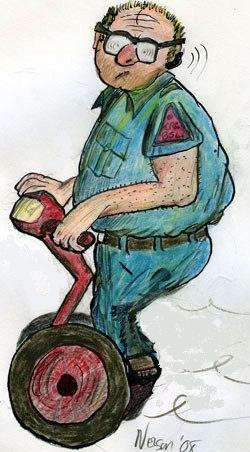
\includegraphics[height=60mm]{corps/chapitre2/img/timothee1.jpg}
\end{floatingfigure}

Outre l’ex-bibliothécaire Bea Bellow, Anglo-Gaspésienne sans défense qu’essaie d’agacer Dart Vader, personne ne porte attention à sa remarque. Ni les joueurs de 500, ni la vieille téléphage, ni Timothée-Milet Tardif, surnommé le Motté, qui, juché sur un ancien Saguewanish, clone saguenéen de la populaire trottinette Segway, vient faire sa tournée d’inspection.

Comment l’avait-on affublé d’un tel prénom ? Sa mère Marie Rioux dite la Maririou, voulait l’appeler Dimitri, en l’honneur du compositeur russe Dimitri Dimitrievitch Chostakovitch dont elle appréciait au plus haut point les concertos pour violoncelle. Mais son père, Romain Tardif dit le gelé, suggéra un compromis de taille, soit de s’inspirer du nom de Timothée de Milet. Ce musicien grec de l’Antiquité exigeait en effet que l’on oublie toute formation musicale avant de venir jouer avec lui. C’était un poète avant-gardiste qui détestait emprunter les sentiers battus. En outre, n’avait-il pas fait ajouter quatre cordes à la lyre grecque ancienne, la kithara, parce que onze possibilités sonores, au lieu de sept, pouvaient offrir un meilleur plaisir harmonique aux spectateurs ? Paradoxalement, Romain, un athée devenu anticlérical, et Marie, une non-croyante finalement apaisée, ignoraient qu’en grec, Timothée signifiait «Celui qui craint Dieu».

- Yo chef, c’est-y aujourd’hui que tu nous fais livrer du chinois ?

En voilà un qui ne peut vraiment pas s’habituer au manger mou, se dit l’employé en saluant Gagnon de la tête. Mais qui le pourrait ? Comment peut-on y arriver ?

À 43 ans, Timothée est un binoclard en passe de devenir chauve, un binoclard rendu grassouillet, même des seins, des cuisses et du fessier. Comme une femme. Il sait qu’il devrait cesser de toujours utiliser sa bécane électronique et marcher davantage dans les longs couloirs de l’institution, ou encore, faire comme ses parents et s’en remettre à un exerciseur de marche. Mais bon, à quoi cela servirait-il ? Quel sens cela aurait-il ? De toute façon, il finira, à son tour, dans un des casiers frigorifiés du sous-sol !

L’homme est chef de section classe 1, un CS-1 comme il se dit dans le milieu. Huit heures par jour, il traîne sa dégaine au Centre régional gériatrique du Bas-Saint-Laurent, alias le CRG-BSL, un établissement rimouskois relevant du ministère des Affaires gérontologiques (MAG), où il est responsable de sept salles gériatriques, de grandes pièces aussi éclairées que le salon communautaire, pour peu qu’on veuille bien ouvrir les stores, source constante de conflits. Là, des personnes âgées, déprimées ou neutralisées, autonomes ou moribondes, y vivent, y végètent, y reposent, y meurent. Plus aucune ne rêve. Il n’y a pas de lit vacant; aussitôt vidés, aussitôt remplis.

Cela ne signifie pas que Timothée soit gériatre ou gérontologue. Il ne dispose que d’un certificat collégial en technique informatique. Son travail est plutôt de voir à ce que tout turbine sans histoire dans son département. En cas de pépins, il a accès à des ressources professionnelles, pour peu qu’il sache qui aller lécher dans le bon sens du poil ou, parfois, qui aller arroser d’un bakchich approprié. En ce sens, il est payé pour coordonner. Pour que tout balance. Tant de vieux, tant de lits, tant de fichiers informatiques.

- ’Tention le Motté ! On pousse de la viande froide !

Timothée regarde passer les deux préposés du grand frigo venus prendre livraison du père Morneau dont l’agonie avait été aussi rapide qu’imprévue. Était-ce encore une fois l’œuvre de la «pilule du bonheur», cette cause relativement fréquente de mortalité qui, officiellement, n’existait pas ? On ne pourra sûrement pas se fier sur l’autopsie pour le savoir; une telle pratique n’était plus requise dans le cas de ces décès survenus dans le respect des normes et à l’intérieur du cadre établie. À moins, bien sûr, que quelqu’un ne l’exige formellement.

Emballé dans un sac mortuaire, le cadavre du misérable a été placé sur un chariot brinquebalant dont les couic couic signalent un déficit inquiétant du côté lubrifiant. Le funèbre convoi file vers le No Man’s Land faisant la jonction entre les sections Nord et Centre du 5e étage. À cet endroit, le corridor s’élargit en salle d’attente avec, en son milieu, sur une table du siècle dernier, un terminal de quanticordi. Le père Morneau et ses misères terminées doivent le contourner pour pouvoir accéder aux ascenseurs, ce qui distrait, le temps d’un plissage de front, Steeve Desrosiers, l’arrogant chef de section (CS-1) du 5e Centre. Carriériste sans vergogne, il est occupé à initier un nouvel employé.

Quel tableau ! Près du mur, un sac mortuaire et deux taupins qui jouent à ceux qui n’entendent rien pour cause de réalité. Plus au centre, un terminal quantique et deux officiants qui jouent à ceux qui ne voient rien pour cause d’avancement.

À grand renfort d’effets holographiques, un document promo présente le CRG-BSL comme étant la onzième merveille du monde, «l’édifice intelligent le plus sophistiqué à l’est de Québec». Au travers des inepties du publireportage, on apprend qu’il a été érigé sur les ruines d’un ancien centre commercial démoli, pour des raisons de sécurité, en 2021. L’immeuble de sept étages est subdivisé en trois pavillons : nord, centre et sud. Tandis que le sous-sol, le rez-de-chaussée et les deux premiers étages accueillent les différents services essentiels au bon fonctionnement de l’établissement, les cinq niveaux subséquents sont propres à l’hébergement des pensionnaires âgés. Sur ces étages, on y a structuré la vie et sa logistique en trois sections pouvant accueillir chacune, un maximum de 56 bénéficiaires, dont certains provisoirement vivants, et parfois, pour de très courts séjours, d’autres déjà trépassés. Ainsi, à pleine capacité, le CRG-BSL peut accommoder 840 personnes âgées. Timothée hausse les épaules.

- 840 petits vieux en attente d’un grand sac noir à fermeture éclair et d’un dernier voyage sur un charriot qui fait couic couic.

Plus dans le détail, peut-on voir en animation idéalisée où tous les bénéficiaires sont, bien entendu, souriants, chaque section compte sept salles de huit lits chacune, un salon communautaire, une «petite chambre» pour certains besoins … intimes, un poste de garde et un bureau pour le CS-1. Ainsi, les quatre premières sont des salles communautaires pour personnes autonomes (SC2PA), des locaux communément appelés 2P où les préposés n’entrent quasiment jamais. Deux de ces salles sont réservées aux dames, des 2P-F, et deux sont prévues pour ces messieurs, des 2P-H. Les pensionnaires y sont généralement en bonne santé, en tout cas, ils le sont pour un certain temps, et ils s’y débrouillent généralement seuls.

- Dans les pires cas, ajoute Desrosiers, ce qui est assez fréquent, ils sont dépressifs, colériques, violents, voire même anorexiques. Quand cela se produit, il faut les soulager et, surtout, les stabiliser par médication appropriée que l’on ajoute mécaniquement à leur alimentation quotidienne.

La recrue ne semble pas avoir compris le sens de ces «ajouts mécaniques». Mais Timothée en a assez entendu et fonce en direction opposée. De toute façon, la voix de Steeve Desrosiers l’a toujours irrité.

Sa boucle d’oreille, chef-d’œuvre de miniaturisation qui cache un dispositif personnel polyvalent (DPP), lui chatouille soudainement le lobe.

- 5e Nord, Timothée Tardif !

- As-tu des morts depuis la fin de semaine, demande la voix désagréable du directeur de l’hébergement, Jean-Pascal Lemoignan.

- J’ai un bénéficiaire de Cabano, Albert Morneau. Ils viennent de partir avec. Mais le système informatique est en panne. Fait que …

- J’sais, j’ai r’marqué ! Quand tu pourras !

Lemoignan a raccroché sans avoir son rapport. Mais il l’aura, il le faudra bien. Tant de morts, tant de vivants, tant de lits, tant de tables, tant de fichiers, tant de verres d’eau. Des statistiques, des colonnes, des justifications, des analyses, des mémos où il n’y a jamais place pour la vie vécue, celle des amours, des peines, des joies, des colères, des coups de chance, des coups durs. Et le CS-1 ne devra surtout pas parler de sa perplexité, de ses soupçons, de cette improbabilité qui caractérise la fin d’Albert Morneau, de cette présomption qu’il pourrait y avoir eu recours à la pilule du bonheur ! On lui ferait reprendre son rapport.

- Que des faits, Tardif, que des faits, lui dirait-on.

Dans les trois autres dortoirs dont Timothée est responsable, c’est une tout autre histoire. Tout d’abord, les deux sexes y sont confondus. Perte de conscience ou d’autonomie aidant, il n’est plus aussi important de garantir l’intimité. À quoi cela servirait-il, n’est-ce pas ? Car dans les cinquième et sixième pièces, des salles communautaires pour personnes en perte d’autonomie (SC3PA), c’est-à-dire des 3P, on loge des hommes et des femmes qui ne peuvent plus demeurer en 2P, des cas devenus séniles, poqués, problématiques, incurables. L’une est conçue pour les cas mineurs, la 3P-M, l’autre pour les cas plus lourds, la 3P-L.

Enfin, le dernier local appelé par dérision, surtout aux CRG de la région montréalaise, EOR («End of the Road»), est un mouroir identifié en signalisation interne comme étant une salle palliative (SP). On y place les incurables qui n’en ont plus que pour quelque temps, ainsi que les moribonds. Il arrive que l’on doive y rajouter un lit ou deux.

Même s’il essaie d’aller le moins vite possible, Timothée est bien conscient que son Saguewanish est trop bruyant, comme vient de lui rappeler cette coquette de 84 ans en jaquette rose, dont le sourire lubrique n’a d’égal que la tenue hétéroclite.

- Je sais Madame Bérubé, faut que je m’en occupe.

Sûrement un problème d’insonorisation sur le bloc moteur. Mais, bon, le modèle qu’il chevauche n’est plus sur le marché. Il fait partie d’un lot de trente-cinq trottinettes d’occasion achetées à l’ouverture du Centre, il y a cinq ans de cela. Et, c’est connu, l’Administration n’a pas les budgets nécessaires, du moins pour l’instant, au renouvellement de sa flotte de bécanes. Il va falloir patienter.

Dans une 2P-F où il vient d’entrer, une scène l’interpelle. Sans hausser le ton, comme s’il émettait une prière secrète, il dit en direction de deux coquines, l’une surtout grassouillette, l’autre surtout fripée.

- Regagnez votre lit, Madame Thériault. Si vous n’arrêtez pas votre petit manège, j’vais être obligé de faire un rapport sur votre homosexualité. Ils vont vous attraper et vous déménager chez les foqués du sous-sol. Et vous connaissez les gardiens !

Pour ne pas voir le résultat de son intervention, il fait un rapide tour de la salle en se demandant comment une chambrée de vieillardes pouvait en arriver à sentir aussi mauvais.

- Méchant moteur là-d’dans, mon Motté, lui signifie, un peu plus loin, près du poste de garde, un petit vieux en robe de chambre.

- Va b’en falloir que je l’amène au garage, Monsieur Jean, lui répond Timothée, viscéralement agacé, même si rien ne paraît.

Si le bonhomme l’a appelé Motté, c’est qu’il a des liens avec certains employés qui ont une opinion bien précise sur Timothée. En existe-t-il seulement qui n’en ont pas ? C’est comme ces vieillards de tout à l’heure, attablés au 500 dans le salon communautaire. Aucun d’eux ne l’a salué. Tous l’ont ignoré. Ils ne lui auraient parlé que si nécessaire. Pourtant, ce n’est pas là l’effet d’un complot, mais plutôt le reflet d’une culture, celle des Boomers. Toute leur vie, ces gens ont méprisé l’autorité. Ce n’est pas sur leurs vieux jours qu’ils commenceront à agir autrement. Sale génération !

Une forte odeur d’ammoniac rappelle au chef de service que la veille, un des pensionnaires, André Maheu, a eu un «accident» en plein milieu de la pièce. En plein dimanche après-midi ! En pleine journée des visites alors que certains «parents autorisés» ont le droit de venir aux étages s’asseoir, pendant une heure, devant un proche institutionnalisé en 3P-M (salle pour cas lourds) ou SP (salle pour moribonds). Pas en 2P (autonomes) ni en 3P-L (poqués légers). Les pensionnaires de ces milieux de vie doivent descendre au rez-de-chaussée dans le grand salon où les visites sont tolérées entre 13 h 30 et 16 h 30. Pas chanceux, le père Maheu ! On l’a depuis mis aux couches, ce qui signifie, pour lui, un transfert imminent en 3P. Mais, bon! C’est la vie !

Timothée fait faire volte-face à son Saguewanish et met le cap sur la lourde salle SP.

- Chef, chef, fait une voix suppliante

Diane Loubert, une septuagénaire qu’on dirait nonagénaire, est une ancienne fonctionnaire du ministère de l’Agriculture qui n’eut de vie que celle de ses registres de cheptel. Aujourd’hui, elle traîne ses savates dans les passages du CRG, rêvant de bovins broutant à l’infini et de fermes laitières s’étendant par-delà l’horizon.

- Je n’ai plus de sacs pour ma colostomie.

- Je m’en occupe, Mme Loubert, répond Timothée en «double tapant» sa boucle d’oreille, question de numériser la demande.

C’est vrai que sa bécane est vraiment bruyante, se dit-il en observant le dos voûté de la bonne femme condamnée aux affres d’un anus artificiel. Reste que bruyant ou non, pouvoir se promener en Saguewanish au lieu de marcher, marcher et marcher dans un établissement de santé long à ne plus finir comme le CRG-BSL, c’est tout un progrès. Justement, le foutu progrès s’est installé à tous les niveaux, du haut en bas de la pyramide, à gauche et à droite de la société.

Timothée connaît quasiment par cœur la propagande gouvernementale, celle concoctée par les émules du docteur Joseph Goebbels à l’œuvre chez le gros Turcotte.

- Poussé par la criminalisation fédérale du tabagisme et des machines à jeux vidéo survenue en 2020, le Québec, dernière province canadienne à le faire, a dû se mettre à la recherche de nouvelles sources de revenus, question d’éviter les déficits budgétaires, une pratique illégale, tout en assumant le coût faramineux de l’entretien des baby-boomers devenus, pour la plupart, octogénaires. C’était vouloir régler la quadrature du cercle, à plus forte raison, que le Fédéral avait, encore une fois, fait faux bond. Il a donc fallu innover, innover pour que la vie redevienne harmonieuse chez nous.

Ce que la machine à lénifier ne disait pas, c’est qu’étant issus des générations X, Y et Z, les politiciens qui avaient à régler ce casse-tête, haïssaient les baby-boomers, beaucoup plus ceux de la phase 1946 à 1954, que ceux de la 1955 à 1965, appelée également «Génération Jones». À tort ou à raison, ils se considéraient comme victimes des Boomers, une nuée de sauterelles qui avait tout pris sans rien laisser, une cohorte de salopards qui ne s’étaient pas donné la peine de leur transmettre, comme c’était leur devoir de le faire, les valeurs traditionnelles de la culture québécoise, avec ses piliers qu’étaient religion et famille, un troupeau de dégénérés sans repentir ne méritant aucune compassion.

C’est ainsi que l’industrie thanatologique, les centres d’hébergement privés pour personnes âgées, les cliniques gériatriques privées, en fait, tout ce qui, du secteur privé, concerne les «aînés», avaient été nationalisés et fusionnés de façon rigoureuse dans le service public, en vertu de la loi 173, dite Loi Turcotte. Cette loi québécoise avait été adoptée dans la foulée d’importants amendements constitutionnels votés à Ottawa, au terme desquels, il n’était resté à peu près rien de la Charte de Droits de Pierre Eliott Trudeau.

Avaient été soustraits à la loi 173, les retraités qui, bardés de REER et de caisses de retraite, ou ayant des enfants fortunés, avaient la capacité physique et les moyens financiers d’habiter chez eux et d’y vivre en bonne santé. Avaient été également soustraits, les membres de communautés ethnicoreligieuses pouvant démontrer, inspections inopinées à l’appui, que leur milieu ethnique, communautaire, sectaire ou religieux les prenait en charge aussi bien que pourrait le faire l’État. C’était là une dérogation bien hypocrite puisqu’aucun DG de CRG ne voulait de Juifs hassidiques, de moines bouddhistes, de cathos intégristes ou de fondamentalistes islamistes, pour ne citer que ces exemples, dans une de ses salles d’hébergement. On imagine les protestations, les exigences d’accommodements et tout le cirque associé. Au printemps 2028, Sylvain Turcotte, ministre d’État à la Réforme des services sociaux et député de Rimouski, avait déposé un vaste projet de réforme en chambre et l’avait fait légitimer par un référendum gagné haut la main en octobre suivant, avec 68,53 % de «oui».

Dissimulé dans un cadre de porte, Dart Vader se touche à la canule.

- Rien qu’une barre de chocolat, chef! J’suis prêt à te la payer le triple du prix !

- C’est interdit, Monsieur Gagnon.

Timothée n’est pas de ces employés qui s’adonnent à la contrebande alimentaire; pour lui, c’est trop risqué; il est quand même CS-1. Mais ceux qui ont l’audace de déjouer les capteurs électroniques arrivent, semble-t-il, à bien «arrondir leurs quinzaines».

Ce Gagnon n’est pas le seul à vivre de petits espoirs, à rechercher, malgré tout, les soubresauts de vie. Nombreux sont ceux qui n’ont pas encore atteint le degré de résignation nécessaire à la bonne marche administrative et logistique du Centre, ou le degré de désespoir nécessaire à la quête d’une «pilule du bonheur». Peut-être qu’aujourd’hui, avec de la chance, si tout fonctionne comme souhaité, si les planètes ont le bon alignement, ils dénicheront une vraie pomme, une Cherry Blossom pas complètement mangée, un sac de pinottes à moitié plein, deux tranches de pain pas trop sec, un fond de Crunchy Nature ou, peut-être, une petite poignée de caramels mous. Peut-être recevront-ils la visite d’un fils, d’une fille, avec ou sans leur progéniture, qui leur glissera un livre, une barre de chocolat, un sac de croustilles au vinaigre, un fromage au lait cru, quelques films en format mini 3DVD ou de quoi se crémer leur vieille peau sous les plis ? Peut-être que leurs hémorroïdes, leur herpès génital, leurs ulcères buccaux ou leur torticolis ne les rattraperont pas ce mois-ci. Peut-être, peut-être … Pour ces gens, ce sera, plus que jamais, «un jour à la fois», puis une semaine, un mois, un an, cinq ans !

Effectivement, cinq ans s’étaient passé depuis le «Oui» au cours desquels le gros Turcotte était devenu vice premier ministre et président du Conseil du Trésor. On l’appelait «l’homme fort de Rimouski» ! Mais dans le fond, ce fils de cultivateur au pif couperosé, aux énormes doigts velus, aux mollets d’haltérophile traité et à la panse de sumo, n’avait fait que poursuivre la Réforme de la santé enclenchée quelques années auparavant, une révolution administrative où on avait notamment aboli l’Assurance-maladie et l’Assurance-médicaments pour les sans-emploi. On imagine les économies! En conséquence, les assistés sociaux, les conjoints au foyer et, surtout, les retraités avaient dû retourner sur le marché du travail, question de redevenir en situation de payer leur juste part d’impôt et, du coup, de pouvoir redevenir «assurés».

Malgré la distance, Timothée entend la voix pédante de son collègue du 5e Centre en train de tout expliquer au jeune préposé.

- C’est un principe actuariel fort simple, articule-t-il. Il faut qu’en tout temps, l’impôt payé compense, à tout le moins, les coûts des services gouvernementaux reçus. C’est là une pratique obligatoire en vertu de la Loi québécoise sur les équilibres budgétaires promulguée en 2016. Depuis, le gouvernement gère de façon très serrée et toute coupure est la bienvenue; les gens sont même incités à faire des suggestions.

Un peu plus et le nouvel employé prendrait des notes. Pourquoi le son porte-t-il autant dans ces grands couloirs ? se demande Timothée.

- En corollaire, poursuit l’exécrable Desrosiers, toute nouvelle façon de faire des sous avec les services est, elle aussi, la bienvenue.

Son visage devient rayonnant.

- Régulièrement, avec grand déploiement médiatisé, la ministre du Revenu Eleonora del Campo remet des certificats de mérite aux citoyens dont la suggestion a été retenue. Personnellement, soit dit en passant mon jeune ami, je trouve que c’est une femme délicieuse et très séduisante. On ne croirait jamais qu’elle est une politicienne.

Comment le faire taire ? Surtout que cet idiot passe sous silence la pénible période qui a précédé la Loi Turcotte. Timothée qui était au ministère de la Santé se rappelle très bien le «trou» qu’avait généré la Réforme, un «trou» qu’on pourrait qualifier de démographique. Il avait été prévu que dans les cas d’incapacité de retour au travail, les assistés sociaux tributaires d’une maigre allocation mensuelle émise par l’État, les conjoints déconnectés du marché du travail ou les personnes âgées trop fatiguées pour exercer un emploi, pouvaient faire affaire avec une clinique de jour comme il y en avait partout où, moyennant de menus travaux, on leur servait deux repas par jour et on leur permettait d’accéder gratuitement à un médecin salarié de l’État.

Mais le poids démographique des baby-boomers étant ce qu’il est, trop de vieillards se retrouvèrent en même temps dans ces cliniques de misère. D’où la suite que l’on confia au ministre Turcotte avec sa Loi 173, celle qui institua les CRG dans chaque région administrative du Québec, sauf à Montréal où il y en a eu quatre et à Québec, deux. C’est de cette façon que les Boomers furent extirpés de leur sordide condition.

La porte de l’ascenseur s’est ouverte et Jean Saint-Gelais, un snoreau impénitent, apparaît avec son escorte de préposés.

- Tiens, si c’est pas le chef, grince le vieillard.

Timothée lui lance un sourire.

- Monsieur Saint-Gelais, bon retour.

- Ton ami Desrosiers est en train de se former un nouveau «screw» ? répond-il en pointant vers le 5e Centre.

Le bonhomme vient de passer un mois en réclusion au sous-sol pour trafic de chocolat Cadbury, d’où le recours à un terme méprisant normalement attribué à du personnel carcéral. C’est un voisin dans sa 2P qui l’a dénoncé. Un voisin imposé par le système. Quelqu’un que l’on déteste, mais avec qui ont est tenu de cohabiter dans une petite salle. Cela, jusqu’à plus soif ! À l’exception de cas extrêmes comme cette histoire récente de voisins de lits qui en étaient venus à s’échanger des coups, on ne peut être muté de salle 2P. Normalement, quand on quitte sa 2P, c’est pour s’en aller en 3P, l’antichambre du mouroir. Et là, c’est fichu.

- Techniquement, ânonne le CS-1 Desrosiers plus loin dans le passage, aussitôt qu’une personne âgée n’est plus en mesure de demeurer chez elle, dans sa maison, c’est-à-dire qu’elle commence à coûter plus cher à l’État que ce qu’elle lui rapporte (la colonne de gauche plus lourde que la colonne de droite), le CRG de sa région la prend en charge, qu’elle le veuille ou non. Ses biens sont liquidés à la satisfaction de ses héritiers, ces derniers se retrouvant imposés à raison de 50 % de la VMEB (valeur marchande estimée des biens) et de 40 % du TLEP (total des liquidités, des économies et des placements). S’il n’y a pas d’héritiers, le fonctionnaire-liquidateur verse l’argent obtenu dans le compte bancaire du nouveau pensionnaire. Cette procédure permet de s’assurer que le loyer sera fidèlement payé, du moins pour un temps.

- 2 500 \$ par mois, c’est ça ?

Le jeune fait montre d’intérêt. Un bon point pour lui.

- Tout à fait.

On se croirait à la radio de Radio-Canada d’il y a 25 ans !

- Une fois logée dans son CRG, la personne doit effectivement acquitter un tarif mensuel fixe de 2 500 \$ non négociable. À défaut de paiement pour un deuxième mois consécutif, la somme due est saisissable chez les héritiers sans avoir à intenter de procès. Évidemment, les baby-boomers étant ce qu’ils sont, il n’y a pas toujours d’héritiers. Auquel cas, advenant qu’un bénéficiaire n’ait d’autres revenus que sa pension du fédéral et celle de la Régie des rentes du Québec, le CRG est contraint de le loger et le nourrir à perte. En jargon administratif, on dit alors de ce vieillard qu’il est un PH, c’est-à-dire qu’il bénéficie du «Programme humanitaire» que chaque centre est tenu d’administrer. Chaque année, le cumulatif de ces pertes est acheminé au ministère de la Santé pour remboursement. Reste que dans l’ensemble, nous affichons, dans les CRG, des résultats très intéressants. Bon an mal an, nos bilans font état d’une moyenne nationale de 42 % de profit, ce qui comble de bonheur la ministre del Campo, une comptable agrée dont la chaste beauté ne cesse de m’émouvoir.

À l’autre bout, Timothée se remémore cette récente altercation entre deux bonshommes, l’un traitant l’autre de «vieux PH», une histoire pathétique qui s’était terminée par une luxation de l’épaule, juste ici, près du salon communautaire.

Monté sur sa Saguewanish, il est cependant tiré de sa réflexion par Solange Gadoury, une octogénaire toute rondelette, le genre à ne pas s’en tenir qu’au pitoyable manger mou, qu’il entrevoit dans la SP, en sérieuse discussion avec un grabataire. Ayant elle-même aperçu le fonctionnaire, elle quitta la salle et le regarde filer.

- Va falloir que tu parles à Monsieur Jones, chef !

Timothée lève le bras en signe d’acquiescement.

Rares sont les retraités qui acceptent de venir s’installer dans un CRG, l’image de ces établissements étant plutôt mauvaise. Ne sont-ce que de grands mouroirs bien organisés où la qualité de vie est assez proche de zéro ? Sauf exception, les volontaires seront des personnes seules, peu fortunées et mal en point. Elles auront très souvent connu des vies dissolues et voudront enfin trouver le calme et la sécurité.

Complètement à l’inverse, il y aura les rebelles, les insoumis. On réfère ici aux marginaux qui, à tort ou à raison, auront chialé toute leur vie contre «le système», quel qu’il soit. Ceux-là devront être conduits manu militari dans un CRG, d’où plusieurs finiront par s’évader. Ils vivront d’expédients, manqueront de tout, demeureront constamment cachés, sur le qui-vive, ne mangeront pas à leur faim et souffriront de malpropreté. Mais ils seront libres. Fiers! Ni dieu ni maître! Viva la Muerte ! On les retrouvera parfois malades, épuisés, presque morts, voire trépassés. Un certain nombre difficile à évaluer de ces «dissidents» se sera réfugié sur Anticosti. Un véritable village de vieillards insoumis aurait été construit à la Baie-du-Renard, anse agréable sise dans la partie nord-est de l’île.

D’où le BAG (Bureau des affaires gérontologiques), une police spéciale dont le mandat est de traquer ces «illégaux», sauf ceux d’Anticosti. Le ministre Turcotte aurait des informations selon lesquelles un très grand nombre d’Anticostiens, des vieillards autarciques ne coûtant absolument rien à l’État, auraient recours à la “pilule du bonheur” advenant un débarquement du BAG. Ce serait là un dénouement terrible, un dénouement impensable à justifier dans les médias.

Quant aux «illégaux» non organisés, ceux qui squattent ici et là dans les villes québécoises, ils n’ont pas accès aux services publics de santé (médicaments, consultation, verres, etc.), ils doivent s’en tenir aux médecines parallèles, aux médicaments naturels, aux magouilles des médecins corrompus, voire à la méditation transcendantale. Les pistes sont multiples et le BAG a souvent la main heureuse. Sans compter que ces insoumis sont à la merci de délateurs présents dans tous les milieux. Timothée songe à Louis-Marc Richard, ce salaud qui habite en face de chez lui sur la rue Crouet. C’est que le BAG fait miroiter des primes intéressantes, des primes jamais en argent, mais en crédit sur certains services gouvernementaux, par exemple, deux mois gratuits dans un CRG quand son tour viendra …

Bref, à l’exception d’une petite minorité en assez bonne condition physique dont le nombre est difficile à évaluer et qui s’est organisée sur la grande île du golfe Saint-Laurent, les vieux Boomers récalcitrants sont à la merci de parents, d’amis, «d’aidants naturels», des gens encore actifs qui arrivent à les nourrir et à en prendre soin. Mais à l’inverse, ils sont des proies faciles pour une nuée d’indicateurs, parfois haineux, qui sont résolus à les dénoncer. Advenant qu’ils soient pris, ils sont enfermés pour un certain temps, dans une section spéciale du CRG de leur région, une section sous haute surveillance que l’administration réserve aux têtes brûlées, aux vieillards asociaux et aux «négatifs» de toute farine. Doit-on ajouter qu’un vent de profond conservatisme a lourdement changé le Québec ?

Et le docteur Goebbels de continuer dans la tête de Timothée.

- L’admission dans un CRG n’a rien à voir avec l’âge. Seuls comptent les états d’autonomie financière et de santé. Tel commerçant pourra officier derrière son comptoir, tel cultivateur dans son champ, tel pêcheur sur son bateau, sans difficulté jusqu’à un âge très avancé, gagnant ainsi sa vie et, de ce fait payant de l’impôt. Mais d’autres, plus marqués par la maladie, par la misère, par la malchance, par leur bagage génétique, ne le pourront pas. Tout cela pour dire que certains, des sexagénaires, des septuagénaires, des octogénaires, arriveront au Centre en assez bonne santé, mais que d’autres, de tout âge également, se verront conférer un statut plus avancé.

Ainsi va la vie !

- Précisons qu’en parallèle, il existe un réseau d’institutions un peu similaires aux CRG, les CRRHH (Centre régional de réadaptation et d’hébergement pour handicapés), les C2R2H. Ces établissements ont été mis sur pieds pour prendre en charge les personnes handicapées incapables de fonctionner de façon autonome et rentable en société. Chaque région du Québec peut compter sur un C2R2HI, pour les handicapés intellectuels, et sur un C2R2HP, pour les handicapés physiques.

Son Saguewanish l’ayant ramené vers la SP, Timothée lorgne un vieillard mal en point, l’occupant du 7e grabat, qui lui fait signe.

- Bonjour Monsieur Jones. Ça va mieux aujourd’hui?

Il s’approche du semi-cadavre et descend de sa trottinette.

- J’ai un petit cadeau pour toi, siffle le bonhomme de peine et de misère en lui prenant la main.

La sienne est froide. Froide et humide. Froide, humide, longue, squelettique et désespérée. Une répugnante main de vieux que Timothée tient quand même avec compassion. Gérard Jones, alias Tit-Gérard, souffre d’un cancer du pancréas.

- Un cadeau? C’est pas encore ma fête…

- J’ai 500 piastres…

Le miséreux pousse alors un bout de papier dans la main du chef de section, une main qu’il n’a pas lâchée. En fixant les yeux incroyablement bleus de Tit-Gérard, Timothée opine alors du chef, met le papier dans sa poche et, avec une pensée pour Solange Gadoury, cette bénéficiaire boulotte qui aime bien arranger ce genre de «petits marchés», il repart sur sa mauvaise bécane. Il roule ainsi pensant quelques dizaines de mètres jusqu’à son bureau, un coqueron sans fenêtres à peine plus grand qu’un placard à balais. Par commande vocale, il appelle son logiciel de gestion personnelle, ce qui l’amène à psalmodier une série de mots :

- First Mohawks Nation Bank ! Épargne ! Transfert ! Oui ! Code d’opération numéro 345-8440TRS-90 ! Oui ! Non ! Quitter !

Sur l’image CLTD que son quanticordi a projetée en avant de sa table de travail, il constate qu’effectivement, 500 \$ viennent ainsi d’être ajoutés à son compte. Ce que voyant, il appelle le logiciel de gestion de l’établissement, un produit lourd, capricieux et inutilement compliqué qui a coûté une fortune à être installé à la grandeur des CRG, et il entreprend de naviguer jusqu’aux données relatives au 7e lit de sa SP où la photo de Gérard Jones apparaît. De commande en commande, il finit par repousser d’un mois la date de la Cérémonie de groupe à laquelle le vieillard a été convié. Tant mieux si le bonhomme arrive à se garder vivant un autre mois. Magouille ? Assurément. Tous les CS-1 s’y adonnent et la direction générale fait comme si de rien n’était.

Une fois par mois, le plus tôt étant le mieux, les CRG tiennent une telle cérémonie à l’échelle de l’établissement, cela sur une plage horaire possible pour tout le personnel impliqué. La célébration a lieu dans une pièce conçue à cette fin appelée «Chapelle ardente». Qui en fauteuil roulant, qui sur une civière, qui accroché à un support de transfusion, les participants proviennent des SP. D’autres sont déjà morts. Ils sont décédés depuis la tenue de la dernière cérémonie et, depuis, ont été tenus au frais. Ils sont néanmoins présents, zippés dans de grands sacs noirs qu’on a placés en ordre sur de misérables chariots.

Conformément au règlement, ces Boomers arrivés à la fin de leur route ont préalablement été dépouillés par leurs CS-1 de tout ce qui pouvait encore servir à l’établissement, montre, jaquette, dentiers, verres, etc. De bien mauvaises langues prétendent que tout ne parvient pas à l’Administration, qu’en cours de routes, certains biens disparaissent.

Ainsi, les verres disponibles sont placés sur des tables accrochées aux murs d’un petit salon attenant à la cafeteria. Les intéressés n’ont qu’à s’y rendre et choisir ceux qui leur conviennent. De temps à autre, un préposé va y mettre de l’ordre en classant les prothèses selon leur force et leur complexité : simple foyer, double foyer, triple foyer, etc. Malheureusement, les problématiques ophtalmologiques plus rares, incluant certaines pathologies évolutives, se retrouvent souvent négligées. Ainsi, sauf exception, on n’opère plus les octogénaires aux yeux. En revanche, les gouttes contre le glaucome, les cataractes et autres maladies sont déversées à tire-larigot.

Même logique pour les dents. Mais ici, il faut oublier le procédé de repousse dentaire, une technique à base d’ultra-sons mise au point aux É.-U. au début du siècle. Comme il faut oublier ces magnifiques prothèses sur implants, une techno de remplacement on ne peut plus efficace. Ici, on est en présence de vieillards incapables, pour la plupart, de s’offrir de tels luxes. Et il ne faut surtout pas regarder du côté de l’État pour y pourvoir à leur place. Depuis quelques années, la partie «dent» des dentiers est faite d’acrylique Hi-Impact, ce qui leur confère une «espérance de vie» d’au moins dix ans. Quant à la partie couleur chair, celle qu’on nomme «gencive», elle est faite en acrylique Hi-Impact RP («haute résistance thermomalléable »), ce qui permet de l’amollir en y injectant, sous chaleur, un liquide démulsifiant à base de nanobactéries. Dès lors, on le laisse refroidir juste assez pour l’insérer sans inconfort dans la bouche d’une personne édentée afin d’y mouler sa nouvelle empreinte. Délicatement, pour ne pas que les dents ne se déplacent sur la gencive, on retire ensuite la prothèse, on l’asperge d’un produit à base de sildenafil et on chauffe quelques secondes dans un petit four à micro-ondes. L’appareil masticatoire est alors prêt pour amorcer sa nouvelle vie.

L’effet pervers est, bien sûr, que tous les porteurs ont des dents identiques. Mais au moins, ils en ont. Le seul problème véritable repose sur le fait que parfois, les utilisateurs ont encore quelques dents résiduelles. On doit alors les extraire pour que la personne puisse bénéficier du service de prêt.

- N’est-ce pas là une pratique, euh, inhumaine ? avait un jour demandé Timothée à son supérieur immédiat.

- Inhumaine? Pas du tout ! Ces gens que l’on dépouille ainsi, sont ceux qui, au moment de la cérémonie, sont soit agonisants, une question d’heures ou de jours avant de trépasser, soit condamnés par la faculté à péricliter sans espoir dans la souffrance et la perte de dignité, une question de semaines, mais rarement de mois. Dans un cas comme dans l’autre, ce sont des morts en sursis qui, en attendant la conclusion ultime, ne peuvent que souffrir, s’embêter et coûter cher à l’État. D’où la rationalisation de leur départ. Il faut rappeler qu’en vertu de la Loi Turcotte, les vêtements, les prothèses et les montres n’appartiennent pas aux bénéficiaires, ils ne leur sont que prêtés. Si la personne âgée n’a plus usage de ses verres ou de ses dentiers pour cause de sénilité, d’agonie ou de décès, il est du devoir des autorités de remettre ces objets en circulation; d’autres pourront les utiliser.

Encadré par le DG et au moins trois gestionnaires du Centre, une spécification du manuel de Régie interne, un officiant de l’État civil lit un discours bien mesuré, remercie les vieillards pour leur participation à l’essor du Québec, serre les quelques mains qui sont encore capables de se tendre et quitte la Chapelle. Deux préposés jusque-là immobiles recueillent alors les passeports et les émetteurs personnels (EP - puce RF montée sur un bracelet, une épinglette ou un pendentif ), documents officiels que les CS-1 ont placés dans une enveloppe transparente épinglée sur le devant de la jaquette des moribonds. Ils ferment ensuite les portes et les verrouillent.

Ce que voyant, l’officiant de l’État civil s’empare des documents amassés et, d’un signe de tête, indique au DG qu’il peut appuyer sur une manette. Clouc ! Un gaz incolore, inodore, indolore, mais impitoyable, est alors émis et tous les officiants présents baissent la tête en recueillement. Au même instant, un timbre se fait entendre dans les haut-parleurs de l’établissement, ce qui, parfois, a l’heur de déclencher des scènes fort déchirantes; certains sentent partir un parent, un ami, et d’autres s’imaginent de la prochaine fournée. En moins de trente secondes, la mort a fait son œuvre et, cinq minutes plus tard, de puissants ventilateurs ont déjà fini de purifier l’air de la Chapelle. Tant et si bien que les deux préposés peuvent y retourner finir leur travail.

Quand on lui avait expliqué ce détail de la réglementation, la Maririou avait eu peine à retenir sa hargne.

- Prêt pas prêt, j’y vas pareil ! Je t’enferme dans j’une chambre à gâche chi tu n’as pas eu la bonne idée de mourir avant ! Toi, le vieux Boomer, tu vas trépâcher à l’heure préchise, à la journée préchise, que les fonkchionnaires ont planifiée. Comme ches naichances au chiècle dernier, dans les jannées 60 et 70, où les femmes accouchaient par provocachion au moment où l’obstétrichien ou le gynécologue en avait fixché le moment dans chon achenda.

En théorie, les corps sont alors inspectés et placés dans un sac noir dûment identifié à leur nom et accompagné d’un code couleur. Il ne reste plus qu’à dégager les cadavres. Sur le côté nord de la Chapelle, une longue chute cachée derrière une porte à peine perceptible sert à les faire glisser, dans le plus grand respect, jusqu’au Centre de tri situé au sous-sol. Là, en fonction des dernières volontés, on sépare les «incinérés» (code couleur rouge), des «enterrés» (code couleur vert) et des «formolisés» (code couleur jaune). On achemine ensuite les trois piles de sacs au bon endroit : site d’enfouissement spécialisé (anciennement «cimetière») pour les Verts, incinérateur pour les Rouges et camion-citerne pour les Jaunes (à noter : advenant qu’un mourant n’ait pas d’idée précise sur sa couleur, on lui suggère invariablement le rouge, l’incinérateur étant intégré au système de chauffage du Centre). Dans le cas de ceux qui l’ont exigée par testament, une cérémonie religieuse ou civile, c’est selon, est organisée dès le lendemain de la CG aux frais des héritiers (pour ce que cela veut dire). Les photos reproduites et encadrées par la famille sont alors exposées pendant 90 minutes à l’heure du lunch. Quant aux corps, ils sont déjà rendus à leur destination finale.

Mais en pratique, Timothée sait qu’il peut en être tout autrement. Dieu du ciel ! Surtout depuis l’arrivée au CRG-BSL du sinistre Dr Bellavance. Chercheur renommé auteur d’un traité psycho gériatrique à l’usage des CRG, cet expert a convaincu les autorités ministérielles de le laisser conduire un projet pilote de ferme hormonale. Ainsi, certains vieillards, ceux qu’aucune famille ne réclame ou qui n’ont pas de volontés ultimes devant être prises en compte, sont traités dans une «cérémonie» à part. En effet, le gaz qu’on leur administre ne les tue pas; il ne fait que les placer en état permanent de mort cérébrale. On transfère alors ces vieux zombis au «royaume» du Dr Bellavance - c’est au sous-sol du CRG-BSL - où ils sont parqués côte-à-côté, dûment harnachés à une impressionnante variété de tubes et de cathéters. En leur injectant diverses substances connues du bon docteur, ces misérables corps se mettent alors à produire certaines hormones parmi les plus recherchées. Lorsque prélevées, une procédure bihebdomadaire, celles-ci sont revendues en toute légalité sur le marché canadien ce qui procure des revenus supplémentaires au CRG. Bref, ces vieillards mis involontairement à contribution participent à l’essentiel équilibre budgétaire de l’établissement. Affirme-t-on !

Autre petite note discordante par rapport aux présentations officielles, les cadavres non détournés par le docteur Bellavance n’arriveraient pas toujours intacts, pas toujours au complet, à destination. Dans certains cas, des morceaux, membres ou organes, encore utilisables - quand il en reste - seront prélevés sur les dépouilles fraîches sans que personne ne le sache ou ne veuille le savoir. Un marché noir bien organisé les fera rapidement disparaître. Tout est prétexte à magouille.

Par exemple, certains vieillards ne veulent pas mourir, en bons baby-boomers qu’ils sont. S’ils ont accès à de l’argent électronique, il leur est alors possible de graisser leur CS-1. Car, doit-on le répéter, tout est corrompu. Effroyablement corrompu. En fait, cet argent électronique, alias la «monnaie à plume», est une contradiction de taille par rapport au système en place. Pour qu’un vieillard soit admis dans un CRG, il ne peut avoir dans son compte en banque, un solde mensuel supérieur au montant de son loyer qui est de 2 500 \$. Pourquoi? Pour la tranquillité d’esprit des bénéficiaires et pour les protéger contre la rapacité éventuelle d’employés pouvant être malhonnête. Dit-on ! Or, puisque le système bancaire canadien est inter relié et, qu’en tout temps, un CS-1 peut accéder en toute légalité au compte d’un de ses bénéficiaires, quelle que soit l’institution, il est devenu très difficile de cacher de l’argent. À plus forte raison que depuis une quinzaine d’années, la monnaie de papier est devenue tellement louche que les gens n’en ont que très rarement. Alors, ils s’échangent plutôt des bouts de code et se livrent à de petits virements P2P (point à point).

C’est là qu’arrivent les Mohawks. Les cigarettes ne rapportant plus, le tabagisme ayant fortement décliné dans la population depuis sa mise hors la loi, les enfants de Pocahontas se sont recyclés dans la finance. Ils ont ainsi fondé une banque, une vraie banque à chartre baptisée First Mohawks Nation Bank (FMNB). Or, prétextant leur statut d’Indiens et jouant sur la blanche hypocrisie des pouvoirs publics, ils n’ont jamais accepté de relier leur information au réseau bancaire canadien. Comme résultat, les comptes y sont vraiment confidentiels. Et puisque les gens de la FMNB sont loin d’êtres des idiots, ils ont compris que s’ils abusaient, par exemple, s’ils se livraient à des fraudes, Ottawa ne pourrait le tolérer et lancerait ses ministères de la Justice et des Affaires indiennes à l’attaque. Tant et si bien que les dépôts faits à cette nouvelle institution financière sont aussi en sécurité que s’ils étaient chez Desjardins. Voilà pourquoi bon nombre de vieillards pensionnaires des CRG y ont placé leurs épargnes; d’où l’expression «monnaie à plumes». Ils s’en servent pour améliorer illicitement leur misérable ordinaire.

Quand les pensionnaires deviennent trop impotents, que la sénilité les gagne à petit feu, qu’ils n’arrivent plus à bien gérer cette «petite caisse» grâce au terminal installé dans le salon communautaire, il leur arrive de confier ce souci à un ami, un bénéficiaire moins poqué qu’eux.

C’est le cas de Solange Gadoury, une ancienne vendeuse de hash et de pot dont les salpingites l’empêchèrent d’avoir une famille. Octogénaire pétante de santé, elle vit au CRG-BSL depuis le début; elle avait d’ailleurs fait des pieds et des mains pour pouvoir y être admise. Pour tout dire, tout lui convient, sauf peut-être, le manger mou, mais ça, c’est une autre histoire. Son grand plaisir, à la mère Gadoury, est de mettre son gros nez rond dans les affaires de ces petits vieux en perte d’autonomie, certains ayant été ses clients entre 1970 et 1984, date où elle cessa de vendre ses drogues douces pour se consacrer à l’élevage de lapins. Moyennant de «petits cadeaux» qu’elle dépose à son compte à la FNMB, elle s’occupe de virer les sommes nécessaires aux pots-de-vin et aux petites délicatesses (par exemple de l’alcool, substance rigoureusement interdite dans les CRG).

Plus loin, dans le passage, Diane Loubert, quitte un instant ses rêves bucoliques et fait signe à Timothée.

- N’oubliez pas mes sacs, chef !

\chapitre{L’âge du Nutrisuz}{Assis dans son officine } {en train de jouer à la dame de pique sur son terminal de quanticordi et de se récurer les ongles, Timothée qui ne pense déjà plus aux sacs de madame Loubert, réfléchit sur sa vie de grand timide qui n’arrive jamais à sourire en public et de pestiféré qui craint ses collègues de travail, ces imbéciles qui le traitent de «Motté» et parfois de «p’tit gros qui saute la grande folle du manger mou». Effectivement, son ami, Shimoune Saint-Pierre, est gai comme phoque et ne se gêne pas pour assumer, particulièrement au Centre nutritionnel où il travaille, son exubérante homosexualité, au demeurant inoffensive.}

Tous deux se sont connus aux réunions du Comité de déontologie de l’établissement où Timothée siège en tant que représentant des cadres de premier niveau, les CS-1, et Shimoune en tant que délégué du personnel de soutien. Comme ils ont tous deux été désignés unilatéralement par la direction générale, qu’ils n’ont absolument pas l’appui de leurs pairs et qu’ils sont les deux seuls participants – un bien grand mot - à trouver les séances surréalistes, ils ont rapidement fraternisé.

Un cyberpsy, personnage de synthèse parfois plus humain que les vrais psychologues, a naguère révélé à Timothée qu’il devait son trouble de personnalité à sa mère, en fait, à la tyrannie de sa mère, la redoutable Maririou. Une Rioux avec un X, une Rioux musicalement virtuose, un air bête qu’on a envie de fesser, une fendante qu’on aime haïr, une grosse tête omnisciente, une force sinueuse, une manipulatrice experte, une inquisitrice qui ferait peur aux Dominicains de l’Opus Dei, une vaginocrate qui n’a, de sa vie, jamais perdu le nord, une écorchée vive qui, au cours des 43 dernières années, a été cruellement privée de fibre maternelle.

Mais attention, c’est quand même lui, Romain, qui a eu l’idée de cet invraisemblable prénom de Timothée-Milet, davantage l’expression d’un antagonisme handicapant ou d’un particularisme peu accommodable, que d’un prénom. Lui, le nono prostré dont on fait les gorges chaudes, il porte le nom d’un fonceur, d’un poète, d’un musicien, d’un réformateur, d’un maître à penser ayant fait école. Timothée de Milet ! Si Dieu existait vraiment, jamais il n’aurait permis tel déprédation d’un grand nom, telle offrande à la méchanceté des hommes de 2033 ! Lui, Timothée, fils de Marie Rioux et Romain Tardif, il n’est musicien que parce qu’on le lui a imposé. S’il est devenu joueur de trombone, un instrument qu’il a appris à haïr, c’est avec une fourche à foin lui piquant le bas du dos.

Il se considère comme un «dommage collatéral» ayant dû apprendre à vivoter sans blonde, cela grâce aux psychosévices de cette terrible femme, ainsi qu’ à la nature de l’air qu’elle a pompé dans sa vie d’éternel perdant et dans celle de Romain, son compagnon des 53 dernières années. En fait, Timothée n’en a jamais eu de blonde, pas plus qu’il n’envisage en avoir. Pas qu’il n’en voudrait pas. Bien au contraire. C’est que pour parler à une femme, pour l’intéresser, pour en arriver à pouvoir lui reparler, il faut savoir quoi dire, comment le dire et quand le dire, même si on n’a rien à dire. Lui, il ne l’a jamais appris. Avec le temps, il s’est résigné au célibat. À la vie de vieux-garçon !

Il compense avec des rencontres holographiques par avatars interposés, une techno Web 4.0 popularisée à partir de 2025 avec la banalisation des ordinateurs quantiques, une façon de faire moins gênante, moins terrifiante que la «vraie affaire». Évidemment, l’onanisme n’équivaudra jamais à la copulation, mais, croit-il, c’est mieux que rien. Cela dit, il se refuse d’imiter certains collègues célibataires, des employés qui ne voient aucun mal à utiliser des grabataires en soins palliatifs, du moins certains qui sans devises à plume, probablement d’anciens Boomers dépravés, n’ont d’autres recours, pour survivre un mois ou deux de plus, que de laisser leur préposé assouvir ses bas instincts. Ces pitoyables loques transforment ainsi leur bouche édentée en avantage. À plus forte raison qu’ils reposent dans un lit monté à hauteur réglementaire pour éviter les blessures cervicales dorsales ou lombaires. Ces prestations de service aussi passives qu’illicites sont cependant passibles de congédiement. Sauf qu’ici, comme en bien des choses, personne ne sévit.

La voix de Dart Vader le tire de ses réflexions morbides.

- J’ai pogné la diarrhée, chef. J’pourrais-t y avoir des bananes ? Ou des fraises ?

C’est le coup classique. Dans un recoin de leur cœur, les vieillards conservent un tout petit morceau d’espérance. Peut-être qu’un jour, ils pourront se mettre sous la dent (ou sous les gencives) autre chose que du manger mou. Timothée se garde bien d’accepter; toutes ses économies y passeraient. Sans compter qu’il se ferait prendre et congédier. Qu’arriverait-il, alors, de ses parents? De Romain bon comme la romaine, de Marie dure comme l’hiver ?

Il la revoit lui dire, alors qu’il était ce gamin attaché sur la banquette arrière de la Toyota:

- Ravale ta nausée, Timothée, sinon le gros méchant Harpeur va venir te manger !

Ou encore :

- Si t’arrêtes pas de chialer, Harpeur va venir t’attraper avec sa gang de conservateurs !

Harpeur ! Harpeur comme «peur», comme «harpie», comme «harpon» ! Comme dans :

- Maman, j’ai peur de cette harpie Harpeur qui veut me harponner !

Ce ne serait là qu’une histoire idiote comme il y en a mille dans sa vie, s’il n’avait pas vieilli avec, dans sa pauvre tête, un croque-mitaine appelé Harpeur et des démons crochus et cornus appelés «conservateurs». Il lui faudra bien des années pour finir par comprendre que sa mère référait ainsi au premier ministre canadien de l’époque.

Shimoune avait bien ri quand il lui avait conté cette anecdote. Mais Shimoune riait tout le temps. Il était heureux, Shimoune. À part Amédée Chicot, son patron qui le faisait bien suer, à part les remarques crues de certains idiots dont il se fichait comme de l’An 40, rien ne le dérangeait vraiment. Grand, mince, fortement musclé et plutôt bien fait de sa personne, il ne craignait pas de brandir là où il le fallait, tous les doigts d’honneur qui s’imposaient, pour traiter qui de droit, sourire en coin, de «trou’t’cul pas baisable», pour amuser les bénévoles de la cafétéria avec les pires boutades sur le Nutrisuz, mieux connu sous le vocable de «manger mou», ou pour braver le courroux de son supérieur avec de très extravagants maquillages. Ce nom de Shimoune faisait partie du personnage. En réalité, ses parents lui avaient plutôt donné le prénom de Shimun en l’honneur de son grand-père maternel, un Bellefleur de Unaman-Shipu, sur la Basse Côte-Nord.

Timothée le soupçonnait d’avoir une vie nocturne bien remplie et, à l’occasion, fort éprouvante.

- Mais ça, mon Momo, lui avait-il seriné, ça fait partie de la vie de tapette. J’adoooore !

\begin{floatingfigure}[l]{40mm}
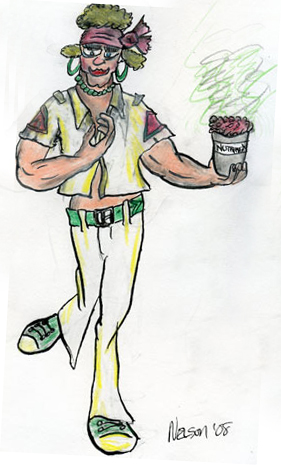
\includegraphics[height=60mm]{corps/chapitre3/img/simon.jpg}
\end{floatingfigure}

Être préposé au centre nutritionnel signifie qu’à raison de trois fois par jour, jamais plus et parfois moins, l’on s’occupe du Nutrisuz, une marque de commerce appartenant à la multinationale Monsanto. Il s’agit d’une nourriture industrielle très économique, une base alimentaire élaborée pour des bénéficiaires âgés, que l’on retrouve à la grandeur des provinces canadiennes et dans plusieurs états américains. Encore une fois, le Québec n’a rien inventé. La trouvaille est plutôt attribuable au docteur Anton Suzkinne, un chimiste d’origine russe faisant carrière chez Monsanto.

Le principe est simple. Tout ce qui est nécessaire pour la santé est présent dans cette purée. On dirait une sorte de gruau sans goût, mais riche en protéines, glucides et lipides, sans oublier un savantissime dosage de produits génétiquement modifiés, auquel on ajoute les suppléments individuels (sur ordonnance), ainsi que les arômes et colorants requis, tous tirés de substances artificielles. Le catalogue de Monsanto fait état de 750 saveurs chacune livrable en moins de 24 heures en contenants de cinq litres.

En cas de contre-indication, il existe du Nutrisuz Base, une nourriture insipide n’offrant que l’essentiel de l’essentiel, auquel (sur ordonnance) on rajoute mécaniquement ce que la personne doit et peut assimiler. Ainsi, le vieillard numéro BSL-34567-98 reçoit un plat de manger mou qui lui est propre, c.-à-d. qu’un voisin ne saurait avaler, un plat vitaminé où ont été incorporés tous les médicaments dont il a besoin. Idem pour les saveurs du matin, du midi ou du soir; la panoplie est assez vaste. Le logiciel choisit au hasard parmi celles qui ont été incluses dans la fiche du bénéficiaire, à sa demande. Cela constitue une petite surprise qui évite l’écœurement et les dépressions. Par exemple, le manger mou du matin sera aux fraises, celui du midi au poulet teriyaki et celui du soir, à la sole meunière. Le lendemain ce sera œufs, poutine cajun et dinde aux marrons. Et ainsi de suite. On a compris pourquoi les arômes et colorants ne pouvaient être d’origine naturelle.

Avec Chicot, un immigrant belge viscéralement homophobe qui le déteste pour le battre, Shimoune est présent cinq jours par semaine entre 8 h et 10 h le matin, entre midi et 14 h, puis entre 17 h et 18 h. En raison du fait que leur quart est divisé en trois blocs entrelardés de creux à rien faire, le CRG les paie quand même pour huit heures, même s’ils n’en font que six. Les vendredis après-midi, Ophélie Marcotte vient se joindre à eux. Préposée à temps partiel, elle assume en sa totalité le quart de fin de semaine. D’où sa présence du vendredi après-midi, question de s’assurer que tout baignera dans l’huile, puisqu’elle sera seule pendant les deux jours qui suivent.

Voilà un arrangement horaire qui laisse bien du temps à l’ignoble Chicot pour poser ses mines, des mines qu’arrive parfois à désamorcer Shimoune et à transférer à son avantage. Ainsi, il y a deux mois, le Belge avait dissimulé les poches de Paxil et de Zyban, des antidépresseurs lourdement utilisés en CRG, afin de rendre le quart d’Ophélie «inoubliable». Quand, à la fin de son premier service, à 10 h. le samedi matin, la jeune femme reçut du système un message selon lequel il n’y aurait pas assez de Paxil et de Zyban pour les préparations de Nutrisuz du midi, elle tenta de joindre Chicot, lequel se fit un malin plaisir de ne pas répondre. En panique, elle communiqua alors avec Saint-Pierre qui, flairant le coup fourré, accourut. Il fouilla dans tous les recoins du centre nutritionnel et finit par repérer les deux poches au fond d’un cagibi à désinfectant.

En clignant de l’œil à Ophélie, il referma l’armoire sans ne rien toucher et appela la sécurité.

- On n’a plus de Paxil et de Zyban pour la fin de semaine, déclara-t-il. Va falloir que j’aille en chercher dans l’entrepôt du sous-sol et moi, j’ai pas le code pour entrer là.

Ce qu’il fit, accompagné d’un agent de la Sécu, lequel, de retour à son bureau dût faire un rapport d’incident. C’est ce qui explique que le lundi matin, Amédée Chicot fut accusé de «négligence en matière d’approvisionnement» sans qu’il puisse se défendre. Eut-il essayé de le faire, il aurait eu l’air un peu idiot; il aurait suffi d’une demande à la Sécurité pour que la Direction puisse visionner la vidéo - car elle existait sûrement - de Chicot en train de fouiner dans le cagibi à désinfectant. Un blâme fut même ajouté à son dossier d’employé. Depuis ce jour, quoi que Shimoune dise, quoi qu’il fasse, la belle Ophélie le trouve génial ! Dommage qu’il soit affligé de mœurs aussi discutables !

Mais doit-on préciser que dans un centre nutritionnel, nul n’est besoin de technicien en cuisine ou en pharmacie ? Un préposé sans qualifications particulières suffit, ce qui est le cas de Shimoune qui n’a jamais terminé son cégep ou d’Ophélie qui s’est spécialisée en poésie innue à l’Université du Québec à Rimouski. C’est d’ailleurs une des raisons pour lesquelles Chicot les déteste tant. Lui, il a étudié des années pour devenir patron de cuisine. Il est passé par de nombreux restos, a servi, toque sur la tête, sous de nombreux chefs, tout cela pour aboutir à 41 ans, dans «le CN d’un CRG de merde», dans un «pays pourri» loin de Montréal, de New York, de Bruxelles. Lui qui se voyait maître queux aussi couru que craint, prépare aujourd’hui du manger mou, cette «putain de saloperie de Nutrisuz à la con», avec pour gâte-sauces, une «lopette» et une «meuf», deux «tarés complètement nuls» !

Car le travail y est désolant. Lorsqu’un bénéficiaire se présente à la cafétéria, salle aux effluves d’eau de javel, il commence par faire la queue au comptoir où l’accueille un assisté social bénévole qui lui capte son émetteur personnel (EP). Le segment pertinent de l’info dont regorge la puce, dispositif essentiel à toute vie, surtout quand on est vieux ou, pire, pensionnaire d’un CRG, est immédiatement traité par le système du CN. Si tout est en ordre, ce qui signifie que le petit vieux n’est pas censé être enfermé au sous-sol ou être décédé ou être grabataire, un timbre se fait entendre. Dès lors, Saint-Pierre ou Marcotte, mais jamais Chicot, place un contenant d’ABS d’un litre sous un périphérique d’ordinateur appelé «malaxeur sanitaire». C’est cette machine intelligente qui y injecte, comme les couleurs chez un quincaillier vendeur de peinture, la bonne dose de Coumadin, de Syntroïd, de Paxil, d’acétaminophène, etc. Le Viagra avait été retiré de la liste un an après le début des CRG, ce qui n’avait même pas soulevé de grogne dans les 2P. Selon les préférences qui apparaissent sur le fichier quantique du bénéficiaire, le Nutrisuz est chauffé ou servi froid. L’opération ne dure que cinq secondes.

Dès qu’il a fini de suçoter son manger mou, le vieux doit aller rincer son plat sous un des cinq robinets d’eau tiède prévus à cette fin. Cela lui permet, juste à côté, de l’emplir d’eau froide, de limonade ou de thé chaud; c’est à son goût. Pour Dart Vader, c’est un de ses moments favoris de la journée. Ciblant bien ses tables, il s’assoie sans attendre d’invitation et, avec une serviette de papier, entreprend de se récurer le «trou» respiratoire. L’impact de son humour est généralement immédiat.

Au fur et à mesure qu’ils ont fini de se sustenter, les vieux qui n’ont rien à discuter, surtout pas le bout de gras, quittent la cafeteria à petits pas mesurés. Mais avant, ils s’assurent qu’un bénévole les décharge de leur plat et de leur cuillère pour les déposer dans une grande laveuse électronique. Là, ces ustensiles sont aseptisés, prêts à servir de nouveau.

- Rappelons que tout le système repose sur les économies énormes que réalise l’État, une machine fabuleuse qui doit pouvoir digérer ses Boomers, avait expliqué récemment le gros Turcotte lui-même. Ainsi, avant la Loi 173, l’activité gouvernementale – je vous parle de l’ensemble des postes budgétaires afférents - qui consiste à s’occuper des personnes âgées coûtait jusqu’à 64 % de plus qu’aujourd’hui. Pour illustrer, on peut prendre l’exemple du CRG-BSL ici à Rimouski, où deux préposés et demi arrivent à sustenter, sans virer fous, plus de 840 bénéficiaires, de deux à trois fois par jour. Un miracle de gestion et de logistique !

Bien beau, mais dans son for intérieur, Timothée ne peut concevoir que l’on nourrisse les gens de cette façon. En ce sens, il est d’accord avec Ti-Dédé, c’est-à-dire Thierry-Ian Dennis-Dubeau (T.I.D.D), le charismatique leader des Verts et chef de l’opposition à Québec, qui, demain, est sensé venir visiter le Centre avec un cortège de journalistes. Évidemment, c’est une pensée qu’il garde bien pour lui; il ne la partage même pas avec Saint-Pierre, surtout qu’il ne le rencontre que dans l’établissement, enclave sinistre où les cafards électroniques sont omniprésents. Pire que dans ce roman de George Orwell dont il a oublié le nom.

On a compris qu’il n’était pas une personne aussi cultivée qu’il ne le souhaiterait. Avant d’être muté au CRG-BSL dans les mois qui suivirent la création de ces établissements, Timothée était agent de bureau senior, un classe IV, ce qui n’était pas rien, à la direction régionale du ministère de la Santé, où, attestation collégiale en poche, il était entré en 2015 à l’âge de 25 ans. Mais auparavant, il avait dû se farcir deux ans d’études en soins infirmiers pour plaire à sa mère; elle exigeait qu’il lui soit utile, «utile à ton tour», disait-elle en tapant du pied. Malheureusement pour elle, il avait dû abandonner cette formation cauchemardesque, étant incapable de supporter la vue du sang. Une petite hémorragie pouvait lui faire perdre tous ses moyens.

Il entend encore sa mère :

- C’est pas si terrible que ça, du sang ! C’est rien que la vie !

Aucune menace n’ayant pu régler sa phobie, il avait bifurqué vers la technique informatique et s’était décroché, sans passion aucune, un certificat en informatique d’affaires. D’où son statut d’agent classe IV. Avec un tel CV, les autorités du CRG-BSL n’avaient pas hésité à lui donner la responsabilité d’une section, la 5 Nord avec ses 56 vieillards, qui plus est, avec grade de CS-1. Quasiment une promotion ! Et même pas besoin d’avoir appris l’anglais !

Un léger frottement sur le cadre de porte de son bureau le tire de sa réflexion.

- Bonjour Madame Bellow, fait-il à l’ex-bibliothécaire avec la même révérence marquée que s’il s’adressait à un ancien allumeur de réverbères.

- Je m’excuse de vous importuner, Monsieur Tardif, mais je n’ai plus rien à lire, sourit-elle en lui présentant de ses deux petites mains ratatinées, quatre livres de poche. J’ai terminé le dernier hier soir.
Timothée s’empare des livres.

- Aimeriez-vous avoir d’autres Giono ? J’en ai trois ou quatre autres, si vous voulez.

- Oh ! Ça sera parfait, Monsieur Tardif. Jean Giono c’est très bien. Très bien même.

- Je vous amène ça demain, Mme Bellow. Mais faut pas le dire à personne, c’est promis ?

- Promis, monsieur Tardif.

Et le fantôme des temps d’autrefois repart dans le silence de ses pantoufles roses.

Ce côté «contrebandier pas méchant» de Timothée ne l’empêchait pas de diriger, depuis cinq ans, une petite équipe de préposés aux bénéficiaires. Ainsi, de 8 h à 16 h, son quart de travail à lui, deux gaillards l’assistaient. Il pouvait s’agir de Steve Grenier ou de son comparse Laurent Bérubé, deux émetteurs de farces idiotes et vulgaires, ou encore de Ronnie Ross - ça se prononce «Wrâné Wrâss» - ou de son complice des coups sournois, Charles Chuck Chicoine - faut dire «Tchok Tchicouaine» - ou encore, d’un petit nouveau appelé Mérovée d’Anjou. Ils étaient donc trois employés, ce qui était amplement suffisant pour s’occuper de sept salles pleines de vieux, dont certains dégoulinant par toute sorte de bouts.

De 16 h à minuit, deux PB venaient prendre leur relève. Personne voulant être de ce quart, Timothée devait produire la liste des affectations au moins un trimestre d’avance. Et même là, certains se vengeaient. Ainsi, ces couches dégoûtantes dans le tiroir principal du bureau de Timothée, ce vieillard oublié trois heures durant sur une cuvette, ce poivre en poudre ajouté au manger mou de grabataires, etc. Enfin, de minuit à 8 h, il fallait se fier au personnel de nuit, des PB comptés sur les doigts de la main qui relevaient de la directrice des soins infirmiers sans avoir de comptes à rendre à Timothée, ce qui convenait parfaitement à ce dernier. Est-on obligé, dans la vie, de multiplier les sources de problèmes ?

À ces gens s’ajoutaient, au jour le jour, des assistés sociaux qui venaient «donner des heures» pour pouvoir manger ou se faire soigner et à qui on confiait exclusivement les tâches dites ingrates : changer les couches dans les salles 3P et SP (aucune couche n’est tolérée dans les 2P; advenant qu’il faille en arriver là, la bénéficiaire est mutée en 3P…), donner le manger mou aux vieillards impotents en 3P et, parfois, en SP, servir le manger mou à la cafeteria, piloter les zambo (sorte de balayeuse, laveuse et cireuse combo) dans les passages et les salles, tondre la pelouse, pelleter la neige, jouer de la musique dans les salons communautaires, pièces réservées aux résidents en 2P et, sur approbation expresse, aux nouveaux en 3P, etc. Et si jamais on manquait d’assistés sociaux, on mobilisait les pensionnaires des salles 2P, cela à leur grande indignation. En cas de force majeure, on avait recours aux bénéficiaires les moins poqués du Centre régional de réadaptation et d’hébergement pour handicapés intellectuels sis deux coins de rue plus loin.

Par sa porte grande ouverte, Timothée perçoit des imprécations en provenance du poste de garde situé à quelques enjambées de son bureau. C’est Laurent Bérubé qui, d’après ce que le CS-1 voit après s’être étiré le cou, est en train de fouiller sans ménagement le bonhomme Martel, un résidant bien malgré lui qui accepte mal sa nouvelle vie de «bénéficiaire». Surtout que son épouse des 51 dernières années est elle-même pensionnaire dans une salle 2P sur le même étage.

- Vous l’avez caché où, votre bouteille, le pére ?

- J’en n’ai pas de bouteille, maudit voyou !

- Vous sentez la tonne à plein nez, vieux menteur !

- M’a t’en faire des «vieux menteurs», espèce de mal élevé. J’vais porter plainte.
Pour ne pas que la scène ne dégénère davantage, Timothée manœuvre sa Saguewanish vers le poste de garde.

- Laisse tomber, Laurent, je m’en occupe.

- Visiblement, le gaillard n’apprécie pas.

- C’est comme tu veux, le Motté. C’est toi le chef !

Et il recule se réfugier de l’autre côté du comptoir, le front plissé de rides malicieuses.

- Venez, Monsieur Martel, on va aller se calmer, fait le chef de section en marchant à côté de sa bécane.

C’est comme s’il avait appuyé sur un bouton, clic ! À coups de paroles courtes et saccadées, le petit vieux se met à déverser l’excédent de son exaspération accumulée. Il en ressort que le CRG-BSL n’est pas une maison de repos pour vieux, mais un abattoir où l’État a embauché des fier-à-bras sans classe, des brutes, des moins que rien, des sans cœur qui séparent les conjoints, qui défont les familles, qui maltraitent les gens, des gens qui ont trimé dur toute leur vie, qui ont payé des impôts comme des idiots pendant une soixantaine d’années, pour finir ravalés au rang de bêtes, des bêtes sans droit «juste bonnes pour attendre la mort».

- Jamais, on ne m’a manqué autant de respect dans ma vie !

Timothée aide le vieillard à s’asseoir sur son lit.

- Monsieur Martel, faites seulement un peu plus attention. La bouteille de rhum que vous cachez dans la poche de linge sale de votre garde-robe, il y a trop de monde qui vous voient vous en servir. Soyez juste un peu plus discret.

- J’en peux plus !

- Si Bérubé fait un rapport, je vais être obligé de donner suite. Vous connaissez la procédure, va falloir vous amener chez les Papyblues. Mais là, faites-vous-en pas, je vais aller arranger ça.

Atterré, le vieil homme reste coi. Timothée a utilisé le mot magique, Papyblues, l’horrible patronyme des tourmenteurs psychopathes qui rôdent dans les dédales du sous-sol.

Hélas ! deux lits plus loin, l’Illuminé démarre son cirque habituel.

- «Malheur à ceux qui de bon matin courent après les boissons enivrantes et qui bien avant dans la nuit sont échauffés par le vin !» C’est écrit dans la Bible, misérables impies ! Et même Saint Luc le dit dans son Évangile : «Car il sera grand devant le Seigneur. Il ne boira ni vin, ni liqueur enivrante, et il sera rempli de l’Esprit Saint dès le sein de sa mère !» Pourquoi ne craignez-vous pas la colère de Dieu ? Vous êtes en train de transformer ce lieu de méditation et de préparation vers la vie éternelle en filiale sordide de Sodome et Gomorrhe !

- Monsieur Savoie, calmez-vous, dit-il à l’illuminé. Monsieur Martel a besoin de se reposer.

Jean-Roch Savoie, un authentique Bleuet d’Alma, s’était établi dans le 3e Rang de Saint-Fabien (25 kilomètres de Rimouski) vers la fin des années 2010. Là, il avait démarré une sorte de secte néo-catholique qui lui avait permis de ne pas trop travailler pendant une vingtaine d’années. Relativement inoffensif, il embêtait néanmoins les autres pensionnaires du 5e Nord avec ses visions apocalyptiques et ses certitudes d’être de plus en plus près d’un Dieu terriblement courroucé par rapport à sa Création.

- Tais-toi donc, espèce de fanatique !

Martel semble pour le moins très agacé.

- Chef, ajoute-t-il, je vais te dire quelque chose, service pour service.

- Vous ne me devez rien, Monsieur Martel.

- Moi, mon ‘tit garçon, je n’ai jamais eu de dettes de toute ma vie ! Écoute-moi bien, j’vas t’le dire juste une fois. Ton Saguewanish a été saboté. Là il fait du bruit, mais fais bien attention, il est à veille de sauter. À ta place, je ne le monterais plus.

- Comment vous savez ça ?

- Je les ai vus faire vendredi passé quand tu es allé jaser dans le bureau d’Alcide. Tu avais laissé ta bécane dans le passage, fait qu’ils en ont profité.

- Qui ça ?

- Il est écrit: «N’abandonne pas un vieil ami, le nouveau ne le vaudra pas !» coupe l’Illuminé. Réfléchis Martel, réfléchis avant de vendre tes frères à Pharaon ! Car il est aussi écrit: «Comme tu as fait il te sera fait : tes actes te retomberont sur la tête».

- Étouffe, vieux sans dessein !

Puis, regardant Timothée:

- Je peux pas de dire ça, chef, tout ce que je peux te dire c’est d’amener ton saguigui au garage.
Au même moment, Timothée voit filer devant la porte de la salle l’ombre furtive de Robespierre Alcide.

- Parlant du loup, fait observer Martel.

Robespierre arrive probablement des commodités. D’où pourrait-il venir pendant les heures d’ouvrage, sinon de là ? Et où pourrait-il aller, sinon là ? Comme on ne le remarque jamais au salon des employés, qu’il mange dans son bureau, qu’il ne fait partie d’aucuns comité et qu’il ne fréquente jamais les fêtes ou les partys, personne ne s’entretient avec lui, sauf Timothée, ravi d’avoir trouvé quelqu’un lui ressemblant quelque peu, façon de parler. Tant et si bien que le personnage est devenu un ami comme l’est Shimoune Saint-Pierre, quelqu’un avec qui il peut échanger.

Inquiété par les propos du père Martel, le CS-1 quitte la salle sans prendre place sur son Saguewanish et, de son petit pas poussif, se dirige vers le bureau de Robespierre, traînant sa trottinette derrière lui.

\begin{floatingfigure}[r]{35mm}
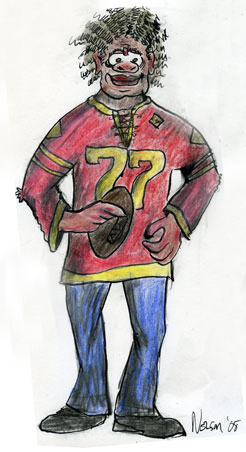
\includegraphics[height=60mm]{corps/chapitre3/img/alcide.jpg}
\end{floatingfigure}

Le grand-père Alcide, un footballeur haïtien (un joueur de soccer, pas de football américain), avait immigré au Québec il y a bien longtemps et, depuis, la famille s’était signalée en sport et en loisirs. Lui, Robespierre, il était directeur des loisirs du CRG-BSL. Fier détenteur d’une maîtrise en éducation physique et d’un bac en récréologie gérontologique de l’Université Laval, il en avait même porté les couleurs au football interuniversitaire. Pourtant, son actuelle fonction avait un sérieux inconvénient pour quelqu’un d’aussi qualifié que lui; au cours des quatre dernières années, on ne lui avait pas consenti de budget. Zéro ! Même pas de quoi acheter deux raquettes de badminton au Dollorama. Les vieux des dortoirs 2P en était réduits à traîner leurs savates dans les salles communautaires, à parler du bon vieux temps, à jouer aux cartes, à regarder la télé, à sommeiller ou, plus rarement, à s’amuser avec le terminal du quanticordi. Le gymnase avait été converti en salon du personnel avec certaines facilités alimentaires et récréatives. Quant à la piscine, on l’avait tout simplement vidée et condamnée.

Puisque le poste de directeur des loisirs est considéré obligatoire dans la Loi constituante des CRG, Robespierre faisait partie des effectifs de celui du Bas-Saint-Laurent et, à ce titre, était tenu d’être présent cinq jours semaine. Le pauvre diable passait ainsi ses grandes journées enfermé dans son bureau, un réduit situé, à la limite des ailes nord et centre du 5e étage, à proximité de l’officine de Timothée. Qu’y faisait-il ? Personne, à part ce dernier, ne savait qu’il y lisait des romans et surtout des ouvrages psychologiques, un dada qu’il cultivait avec délectation, qu’il écrivait de la poésie, qu’il faisait des redressements et poussait des pompes, enfin, qu’il entretenait un monde virtuel où une communauté essentiellement québéco-haïtienne venait revivre les aventures de Toussaint Louverture telles que réécrites et lourdement musclées par Robespierre.

- Tu sais Timothée, lui avait-il raconté un jour, le père de mon grand-père, Terrence-Raoul Alcide, qui était un peu chimiste ou, plutôt, alchimiste autodidacte, avait trouvé une façon de mélanger des herbes, de la levure, de l’eau avec d’autres trucs ignobles. Il faisait chauffer et mijoter cette soupe pendant presque deux jours, laissait décanter et remplissait de petits flacons qu’il vendait dans tous les bars des Gonaïves. Il avait appelé son épouvantable mixture «Pétépano». Il suffisait d’en boire quelques gorgées pour devenir, peu après, en virile situation de fournir, à leur satisfaction, autant de dames que la bienséance communale pouvait l’exiger. D’où le nom «Pétépano». C’est cette trouvaille qui permit à Terrence-Raoul de bien nourrir sa famille et faire en sorte que son aîné devienne un footballeur étoile.

Si Robespierre s’était complu dans une anecdote aussi savoureuse, c’était pour illustrer que chez les Alcide, aussi bien en Haïti qu’au Québec, il y avait une tradition d’entraide. Il fut un temps où toutes les semaines, son grand-père, joueur de soccer, allait porter des caisses de bananes plantains dans un centre communautaire de Montréal-Nord, de la nourriture qu’il avait payée de sa poche. Son propre père, lui-même ailier droit au soccer, mais surtout rappeur et slameur, se produisait gratuitement partout où il estimait pouvoir rendre service à la communauté. Et lui ?

Il n’avait pas répondu. Mais à petits coups de déductions, de mini observations, d’inavouables spéculations et de fines intuitions, Timothée avait fini par l’associer, à tort ou à raison, à la fourniture de pilules du bonheur, un service des temps modernes que Robespierre pouvait rendre à la communauté du CRG.

- Qu’est-ce que je peux faire pour toi, mon ami ?

Le tristounet binoclard s’assied sur la seule chaise à ne pas être encombrée de livres. Pendant cinq minutes, il va tourner autour du pot sans rien oser. Puis, sans transition :

- Tu as sûrement une idée sur ces fameuses pilules qui n’existent pas ?

- Ouais, les pilules du bonheur.

Timothée vise l’ahurissant capharnaüm, plus particulièrement cette masse murale hétéroclite constituée de livres empilés et de souvenirs du Rouge et Or, l’équipe de l’Université Laval.

- J’en cherche. Euh, si jamais tu entends parler de quelque chose …

Il se lève, les yeux sur le souk ambiant, et gagne le corridor sans que Robespierre lui réponde.

Son attention est immédiatement portée vers Luce Morency, une ancienne jolie fille maintenant âgée de 86 ans. Elle s’est encore évadée de son lit de la salle 3P-L 6 Nord, laquelle, heureusement, n’est pas de la juridiction de Timothée. La bonne femme n’a pas ses dents, ses cheveux sont longs, laids, sales et en désordre. Comme elle est nue, sa maigreur pendouillante donne la chair de poule aux gens qu’elle croise. Timothée se pince la boucle d’oreille et dit :

- 6e Nord, code magenta !

On lui répond et il rapporte la fugueuse. Dans l’attente qu’on vienne la chercher, il lui prend néanmoins la main, «venez avec moi, madame Morency», et la fait s’asseoir sur une des chaises près de l’ascenseur. Il en fait autant sur le siège voisin et lui parle du lac Saint-Mathieu où la vieille dame habitait un chalet converti en maison. Pendant une trentaine d’années, elle y avait exploité une petite affaire de location de roulottes rapaillées qu’elle destinait aux villégiateurs venus de la ville. Puis un jour, un de ses amants était disparu avec la caisse, juste avant un dépôt, et moralement abattue, aux prises avec des dettes insolvables, Luce Morency avait fait faillite. Le reste n’avait été que débâcle, désastre et misère noire.

Peu après, un préposé du 6e se pointe, c’est le gros Lavoie, un calamiteux qui mange à tous les râteliers. Tellement qu’il possède trois immeubles d’habitation au Centre-ville de Rimouski. Il a amené un fauteuil roulant et une couverture dans laquelle il drape la mère Morency. En la morigénant comme une pouilleuse, il la roule jusque dans l’ascenseur et ils disparaissent. Quel fils de salaud !

- Je l’ai connue, dans le temps, la Luce Morency !

La mère Thériault qui décidément ne pouvait rater une si belle occasion, brandit son sourire malicieux des grands jours.

- C’est d’valeur qu’elle vieillit aussi mal ! Méchante belle femme, dans le temps ! Dans le temps de nos bals à l’huile du lac Saint-Mathieu. Elle était tout le temps là. Mais on aurait dit qu’elle se méfiait de moi … Pourtant !

Sans plus tenir compte de la radoteuse, Timothée file vers son bureau, question de vérifier si rien qui ne peut attendre s’est affiché, de signaler sa fin de quart au système et de placer son terminal en mode veille.

Quand la cage de l’ascenseur s’arrête au 5e, Marie-Odile Tremblay, une forte femme de 37 ans que l’on surnomme la Bitch, s’y trouve déjà et semble sérieusement occupée à contempler le tableau indicateur. C’est une agente de sécurité sans charme, ni grâce, ni coquetterie, une personne dont on craint la colère, qu’on n’a jamais vue sourire et qu’on croit délatrice active. N’est-elle pas cette flic maison qui a récemment mis au jour un racket de nourriture clandestine, essentiellement du raisin sec, des abricots séchés et des noix, que deux préposés du 4e Centre, des misérables désormais sans emploi, revendaient à des détenteurs de monnaie à plume ?

Timothée n’ose la saluer, même si, depuis quelque temps, il la soupçonne d’être à l’origine de l’avatar avec lequel le sien s’amuse holographiquement depuis une semaine ou deux. La femme tourne légèrement la tête, comme pour le regarder. On dirait qu’elle nourrit les mêmes soupçons.

Mais au moment où les portes se referment, une main brune tout en muscles se glisse à l’intérieur, ce qui enclenche automatiquement la réouverture.

- Je m’excuse, fait Robespierre Alcide. Il est 16 heures et …

Habitué à ce que personne ne s’intéresse à lui, il ne termine pas sa phrase.

Arrivés au 2e, le CS-1 et l’agente de sécurité sortent. Elle parce que c’était SA destination, la Sécurité occupant toute l’aile sud du 2e, lui parce qu’il se croyait rendu au rez-de-chaussée.

- Au revoir, Marie-Odile, déclame Robespierre, un sourire tout craquelé sur le bord des lèvres.

Sans lui retourner sa politesse - une politesse intéressée ? - elle le regarde avec sévérité. Et c’est avec le même air qu’elle fixe cet autre «perdant» qui tente bêtement de s’excuser. Excédée, elle hausse les épaules et file sur son Saguewanish, toutes voiles déployées. Un Saguewanish qui ne fait pas de bruit. Humilié encore une fois, Timothée entreprend de pitonner la console murale de l’ascenseur. Pourquoi Robespierre ne l’a-t-il pas attendu ? À cause de sa requête de tout à l’heure ?

Mais tout près, dans une officine à peine plus grande que la sienne, un sexagénaire à bouc, selon cette mode grotesque qui frappa l’Occident dans les années 2005-2010, lui fait signe de la main avec insistance. Timothée hésite et se pointe le thorax de l’index en hochant de la tête à répétition. L’autre fait signe que oui en répétant son geste. Le CS-1 embraye donc sa vieille bécane. Il sait que cet étrange personnage qu’on ne voit jamais nulle part, lui non plus, est Sébastien Larose, le dernier syndiqué de la Fonction publique du Québec. Tous les autres sont soit décédés, soit retraités, soit devenus cadres.

La formule Rand ayant été déclarée inconstitutionnelle par la Cour Suprême en 2018, Québec l’avait supprimée l’année suivante pour s’éviter un très juteux recours collectif. En conséquence, plus personne parmi les nouveaux employés de l’État n’avait voulu adhérer au syndicat. Le vieux Sébastien était désormais le seul de son espèce. Ce qui signifie qu’en vertu des lois du Travail en vigueur, le syndicat devrait être dissolu par le Lieutenant-gouverneur en conseil le jour où Larose partirait. En attendant, il cumulait les postes de président, de secrétaire, de trésorier et agissait comme assemblée générale. Ne sachant trop quoi en faire, voulant s’éviter une structure patronale syndicale, les autorités du CRG-BSL avaient préféré placer cet énergumène d’un autre âge dans un bureau confortable où on lui foutait la paix dans l’attente de sa retraite, ce qui devrait arriver dans les huit prochains mois. Croyait-on en haut lieu !

- Excuse-moi, mon homme, fait-il un crayon à la main, je cherche un mot de dix lettres, dix lettres, qui signifie «rationalisation administrative efficace» et qui commence par les lettres HO …

Il a prononcé «mon homme» comme seuls les Bas-laurentiens savent le faire. Vouloir respecter le son, il faudrait écrire «mânem».

- Euh ! Dix lettres ?

- Ouin, p’is ça finit par un E…

- Euh ! Rationalisation administrative efficace, attendez …

- Dix lettres.

- Je l’ai. C’est HOLOCAUSTE.

- Ahhh ! Génial ! Merci mon homme !

Timothée ressort du petit bureau et reprend place sur son Saguewanish. Il s’engouffre dans l’ascenseur et le quitte un étage plus bas, en face du portrait couleur de Sylvain Turcotte, l’homme fort du régime libéral. Ignorant quelques quolibets d’usage, il sort de l’édifice et roule jusqu’au stationnement où il aperçoit Shimoune Saint-Pierre presque nu, couché sur le devant de son automobile électrique en train de prendre le soleil de l’après-midi.

- Beau temps pour s’étendre ! T’as fini ta journée, Momo ?

- Ouin.

- Saint-Pierre ajuste ses verres fumés.

- C’est pas de mes affaires, mais je viens de voir le gros Lavoie placer un bout de papier dans ton pare-brise.
- Ah !
Timothée salue son ami et se dirige vers la section du stationnement - c’est la plus éloignée –qui est réservée aux voitures à essence. Effectivement, quelque chose de flageolant a été glissé sous les essuie-glaces de sa bagnole, concentré de rouille construit en 2013. C’est une feuille toute dégueulasse, on la dirait souillée de matières abominables, où on le traite de «gros motté téteux de boss qui, un jour, va se faire casser sa yeule de rat». Sans colère, il chiffonne le brouillon et va le jeter dans un bac à recup trois pas plus loin.

Pourquoi le persécute-t-on tant ? Pourquoi le déteste-t-on tant ? Il n’en est pas certain. Possiblement parce qu’il ne parle à personne, parce qu’il est chef de section, classe 1, parce qu’il ne fréquente pas le club social, à l’instar de Robespierre, de Shimoune ou du vieux Sébastien Larose. Sûrement parce qu’il a une tronche louche avec ses barniques épaisses, ses cheveux trop éclaircis, sa trottinette qui en arrache, sa chemise tachée de sauce à spaghetti, sa dégaine de perdant. Toute cette méchanceté gratuite, cette bête incompréhension, est, la plupart du temps, lourde à porter et, comme c’est le cas présentement, l’emplissent d’un cafard qui l’habitera encore, il le sait, bien après qu’il sera rendu chez lui. Aimerait-il pouvoir se venger, ruer, hurler, frapper, impressionner, susciter le respect, obtenir du gros Lavoie qu’il lui demande pardon ? Peut-être, mais ce n’est pas vraiment dans sa nature.

Sans dire un mot, il place le bruyant Saguewanish dans la malle de la bagnole, quitte le terrain du CRG et prend la direction de Nazareth. En cette fin d’après-midi de juillet, l’air du fleuve rend possible, voire délectable, la chaleur extraordinaire - à Montréal, ils disent «accablante» - qui assaille l’Est-du-Québec depuis quelque temps. Les gens sont partout sur les trottoirs, les balcons, dans les parcs, sur la promenade du Fleuve, sur les pistes cyclables, sur les terrasses. On rit, on sourit, on crie, on s’arrose, on s’attrape, on s’aime, on est heureux. Mais lui, Timothée, il roule plutôt vers autre chose, vers une sorte de tombeau sombre, sale et hostile où l’humidité sera étouffante et, comme c’est de plus en plus le cas, nauséabonde.

- Merde, j’ai oublié les sacs de la mère Loubert !

\chapitre{Trio pour clarinette, violon et … trombone, le 18 juillet 2033}{Les sabots de frein geignant,}{ Timothée se stationne comme il le fait du lundi au vendredi, à la même heure, devant sa maison, une imitation de cottage anglais particulièrement mal réussie. Pourquoi endure-t-il le revêtement de bardeaux d’amiante blancs remontant au siècle dernier ? Ne sont-ils pas cancérigènes ? Pourquoi ne les fait-il pas recouvrir de planches synthétiques ? Il ne le fait pas parce qu’il n’a pas de sous. Il a deux parents, sans oublier leur sale bête de chien-rat, à nourrir, à vêtir, à soigner, à soutenir, à rassurer, à protéger. À cacher !}

Un chatouillement lui titille l’oreille.

- Timothée Tardif !

- Monsieur Tardif ? Allanah Desrosiers de la Caisse populaire de Rimouski, vous allez bien ?

- Euh …

- Je vous appelle parce que votre compte chèque est à découvert de 97,64 \$.

- Ah !

- Vous allez vous en occuper avant demain matin 9 h ?

- Euh …

- Parfait, Monsieur Tardif, au revoir !

L’homme s’escrime quelques instants avec sa portière aux gonds à moitié pourris, réussit à sortir de sa traction américaine et se retourne pour agripper deux sacs d’épicerie, deux «extra-forts jetables et 100 % compostables». Ce faisant, il réalise que Louis-Marc Richard est, encore une fois et comme toujours, en train de l’écornifler.

Du côté fleuve de la très fleurie rue Crouet, il n’y a qu’une maison, celle de Timothée, une construction artisanale de deux étages, sans parler de son prodigieux sous-sol, laquelle fut érigée en 1970 sur la crête de l’à-pic escarpement, avec triple ancrage bétonné sous la chaussée, ce qui nécessita certains accommodements à la Ville. C’était le seul endroit possible du versant nord; plus à gauche, le haut de la falaise est trop étroit et à droite, c’est le terrain du cimetière nazaréen qui débute. Rapidement, l’invraisemblable cottage se métamorphosa en curiosité qu’on vint voir. Du coup, le voisin d’en face perdit sa vue sur le Saint-Laurent, ses couchers de soleil sur la Côte-Nord et sa belle tranquillité.

Lorsqu’il prit sa retraite en 2010, il vendit son énorme bungalow à Louis-Marc Richard lequel, à son tour, commença à détester l’affligeante bicoque qui lui obstruait le panorama. Tellement, dit-on, que tous les jours, il fait une prière pour qu’elle s’écroule sur la voie ferrée au pied du cap et, qu’au même moment, un convoi ferroviaire la pousse sur les battures noirâtres du fleuve.

Quand, il y a dix ans, Richard apprit que l’inquiétante propriété avait changé de mains, il espéra, un instant, que l’acheteur l’améliorerait, l’embellirait, l’arrimerait davantage à l’esthétique ambiante de la rue et de sa dizaine de maisons. Mais non, rien ne se produisit, pas un coup de marteau ne fut entendu. Ses espoirs furent cependant ravivés cinq ans plus tard, en apercevant un fardier y livrer des feuilles de gypse, des panneaux de contreplaqué, du bois en formats variés, une immense fenêtre à espagnolette et tout le nécessaire pour effectuer des travaux majeurs. Mais encore là, ce fut une déception. Tout disparut à l’intérieur.

- Dis donc, voisin, lui avait-il demandé, tu rénoves ?

- Je construis un logement dans le sous-sol.

- Pour toi ?

- Non. Pour louer.

- À des locataires ?

- À des locataires.

- Mais y en a pas dans notre rue !

Timothée lui avait alors tourné le dos et s’en était retourné à ses occupations. Offusqué, furibond, Richard l’avait mortellement haï et, depuis, il ne lui avait plus jamais parlé. Dans un premier temps, il avait bien remarqué qu’une porte d’entrée avait été aménagée sur la façade permettant d’accéder directement au logement. Mais, quelques mois plus tard, elle avait été bouchée, laissant paraître cette affreuse cicatrice que l’on pouvait encore contempler aujourd’hui. Louis-Marc Richard supposait que son vis-à-vis avait changé d’idée pour les locataires – en fait, il n’en avait jamais vu l’ombre d’aucun – et qu’il avait tout simplement agrandi son espace vital. Oui, mais pourquoi ?

Cet étrange voisin qui ne recevait jamais de visite, qui semblait toujours seul et … sans femme, occupait déjà un grand rez-de-chaussée et, par surcroît, un étage assez spacieux pour abriter deux chambres normales. Pourquoi lui fallait-il un sous-sol en plus ? Lui, un célibataire dont la voiture était un outrage à la rue Crouet et la tenue vestimentaire, une illustration de misère noire. Sans parler de ce chien jaune qu’on avait envie de fesser à coups de pied, une bête sournoise qu’il se contentait d’envoyer marcher par GPS quand il y pensait. Étrange ! Bizarre ! À surveiller !

C’est ce qu’il fit, se mettant même à évaluer le volume des sacs d’épicerie que Timothée charriait parfois tous les jours en fin d’après-midi. Comment un homme seul d’apparence aussi modeste, pouvait-il manger autant que les trois Richard réunis, le père et ses deux ados ? Intrigant !

\begin{floatingfigure}[r]{60mm}
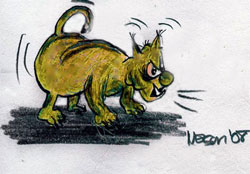
\includegraphics[height=35mm]{corps/chapitre4/img/gazou.jpg}
\end{floatingfigure}

Timothée hausse les épaules et, sacs en main, disparaît à l’intérieur. Sans s’arrêter dans sa tanière, il dévale directement un escalier à pic et tout en bas, cogne du pied. Mais déjà, Gazou l’a repéré et s’est mis à aboyer avec furie, son sale museau de fausset tout plissé par la haine. Heureusement, un ordre susceptible d’intimider un adjudant-chef d’infanterie se fait entendre :

- Ichi ! À côté de Maman !

Instantanément, le chien-rat se tait et Timothée franchit le seuil de la porte. L’un retourne s’écraser près du fauteuil de sa maîtresse, l’autre salue gauchement. Habitué aux senteurs ambiantes, il les ignore et va placer les provisions sur le comptoir de la cuisinette. En passant, il dépose les quatre livres de poche remis par l’ancienne bibliothécaire sur une pile de bouquins non classés.

- Au moins, ils ont sorti les vidanges, remarque-t-il.

À son père qui l’a suivi pour l’aider, il glisse un petit dix onces de vodka que le bonhomme a tôt fait de cacher dans une armoire. Puis, à voix basse

- L’écornifleux m’a encore guetté.

- Penses-tu qu’il commence à soupçonner quelque chose ?

La question reste sans réponse. Comment savoir ? S’il y a danger d’être dénoncé, ça ne peut venir que de Louis-Marc Richard. Les autres résidents de la rue sont trop éloignés pour remarquer quoi que ce soit, pour se douter de quelque chose. Et, en dix ans, mis à part Richard, personne ne lui a jamais adressé la parole, personne n’a jamais paru s’intéresser à lui, personne n’en a eu besoin.

- Merci pour tout ça, Timothée-Milet.

Quand son père l’appelle ainsi, c’est qu’il est heureux de sa présence et qu’il a envie d’échanger, de raconter, de rire.

- As-tu vu, vous recommencez à avoir des fourmis, fait le fils en écrapoutissant trois bestioles prises en flagrant délit d’écorniflage sur le comptoir.

Le vieillard se tord les maxillaires en un sinistre bâillement et s’en retourne s’écraser dans son fauteuil malgré la Maririou qui psalmodie son habituelle liturgie. Elle en a long à dire. Mais Timothée ne l’écoute pas lui non plus. Il garde plutôt les yeux fixés sur cette immense fenêtre pleine de lumière d’où il peut voir le fleuve évoluer autour des îles Canuel et Saint-Barnabé. En même temps, il pense à tous ces gens heureux qu’il a croisés en route. À ces filles qui riaient. À ces filles écourtichées et immodestes qui vivaient débordantes de santé, de jeunesse, d’insouciance. Finiront-elles comme Luce Morency ? Allez savoir ! Mais dans ce coq à l’âne onirique, le masque hargneux de Louis-Marc Richard, une figure fielleuse, toxique, mortelle, vient durement chasser celui triste et perdu de la démente. Et voilà qu’à son tour, il cède la place à celui du bonhomme Martel et à ses insinuations sur son Saguewanish, puis, swoosh !, aux traits tout en sourire, en simplicité et en politesse surannée de Bea Bellow.

Bea Bellow, les Giono ! Timothée a tôt fait de repérer les livres promis sur un des rayons à gauche de la fenêtre.

\begin{floatingfigure}[l]{40mm}
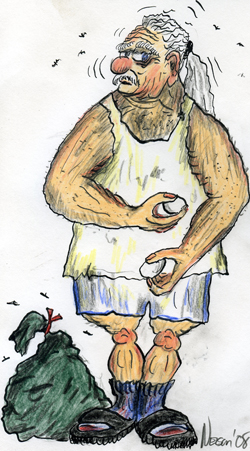
\includegraphics[height=60mm]{corps/chapitre4/img/romain1.jpg}
\end{floatingfigure}

Pendant ce temps, chattemite incorrigible, Romain augmente subrepticement le volume de son écouteur sans fil; l’heureux homme n’entend plus le flot récriminatoire de sa conjointe; savoir utiliser son expérience à bon escient constituerait, dit-on, une preuve d’intelligence. Timothée, lui, a droit au grand jeu. Il a mis trop de temps à revenir de son travail. Il a traîné. À quoi a-t-il pensé ? Voit-il une femme ? On espère bien que non ! A-t-il bu ? Eux autres, les vieux, ils commençaient à s’inquiéter ! Qui peut prévoir une descente de police ? Le BAG frappe toujours sans prévenir. Et patati et patata.

Puis voilà que soudain, sans qu’on ne le sente venir, elle se tait. Consciente de célébrer un cérémonial essentiel à sa vie, elle se saisit du violoncelle debout près de son fauteuil. C’est le signal ! Immédiatement, Gazou file se cacher sous un lit et les deux hommes, résignés, vont au placard chercher leur instrument, le fils un trombone, le père une clarinette.

- Trio pour clarinette, violonchelle et piano, opuch 2 de Vinchent d’Indy, chuinte la mère. Pis toi. Gajou, tu te tais, sinon tu vas avoir affaire à Maman !

Avec son trombone, instrument qu’il déteste de plus en plus et qu’il a cessé de maîtriser depuis belle lurette, à preuve les couacs intermittents, Timothée suit sans plaisir la partition bricolée par sa mère, faute d’avoir un piano. Mais il finit néanmoins par se rendre au bout. Avec son trombone, il ne peut évidemment rendre justice à l’opus original qui a été composé pour clarinette, violoncelle et piano. Il le sait. Et sa mère aussi. Sauf que cette contrariété lui donne une occasion supplémentaire pour se dire déçue de ce fils paresseux, un enfant qui avait tellement de talent musical, tellement de potentiel. Une nouvelle litanie est lancée et sur le point de passer au crescendo. Mais Romain en a assez; il s’immisce.

- Là, tu vas arrêter. Je te rappelle que Timothée, un «travaillant» du CRG où on garde les vieux comme nous autres en cage, nous cache ici, dans sa maison, et paie tout de sa poche. S’il se fait prendre, il est fini pour le reste de ses jours. Tu vas lui sacrer patience. Ça n’a pas de maudit bon sens !
Marie se tait. Elle regarde fixement son homme, puis, façon d’admettre qu’elle a eu tort, elle baisse la tête vers Gazou qui est revenu et qui gronde en direction du vieillard. Ignorant Timothée, elle se lève et marche, l’animal grotesque à sa suite, jusqu’à la cuisine. Peut-être qu’elle va y apercevoir quelques fourmis et se défouler sur les malheureux hyménoptères, se dit Timothée. Mais, au son, elle semble plutôt vouloir bardasser. Il lui faut ramasser la vaisselle du midi et préparer le repas du soir.

Avant, Romain ne rouspétait jamais. Il laissait toujours «border», ce qui convenait parfaitement bien au caractère invivable de la Maririou. Mais, avec les années, il lui a fallu réduire, raréfier, puis arrêter sa consommation de hash; la substance ne lui réussissant plus, le bien-être ayant été remplacé par la paranoïa et l’angoisse. Pire, il y avait eu l’été 2027 et cette affaire ratée depuis laquelle, tous deux étaient reclus. Voilà qui suffit amplement à changer un caractère.

Ému, le fils se lève à son tour, va ranger son instrument, caresse timidement l’épaule de son père en passant et, escorté par Gazou qui essaie vicieusement de lui mordre un mollet, s’engage dans l’escalier.

- Couché Gazou, méchant chien !

Et si jamais Robespierre Alcide lui fournissait les petites pilules du bonheur, ces cachets sans lendemain, qu’en ferait-il ? Comment aborderait-il la question avec son père, avec la Maririou ? «Tenez, avalez ça avec un verre d’eau. Ne craignez rien, ce n’est pas souffrant, c’est comme un somnifère, un gros gros somnifère ! Un somnifère pour toujours !» N’y a-t-il pas une autre solution ? Une façon différente de vivre ? Ça n’a plus de bon sens. L’agressivité, la vindicte, l’acrimonie semblent en escalade constante. Et leur aire d’habitation aux vieux, elle mériterait un grand ménage au savon fort, au plâtre, à la peinture, une rénovation importante avec des rideaux neufs, des meubles moins cabossés. Ça sent mauvais, c’est sale, humide, étouffant, déprimant.

Il est vrai que sa mère tire souvent de trop gros boulets sur de trop petites cibles, mais quand même. Il faut comprendre le contexte pénible dans laquelle elle vivote depuis six ans. C’est comme si on avait mis en cage une lionne de la savane, une lionne dans la force de l’âge avec le museau taché de sang. Pour une personne qui, comme elle, en menait large dans l’univers culturel de la région, la situation est carrément invivable. Et c’est ainsi depuis six ans !

Jeune fille volontaire, opiniâtre, studieuse, travailleuse, bûcheuse, non diplomate, incapable d’humour, toujours sérieuse et, généralement, insupportable, elle s’est retrouvée en 1972, elle avait 21 ans, Premier Prix du Conservatoire de musique de Québec en violoncelle. Ensuite, elle a joué comme remplaçante avec l’Orchestre symphonique de Québec, ainsi qu’avec la Société de musique contemporaine du Québec. De là, elle est passée en France où, avec son caractère éprouvant, elle a bourlingué un peu partout, mais surtout dans le Midi. Des gens ont pleuré à cause d’elle, aussi bien par amour que par haine.

Puis, à 29 ans, elle est revenue au pays lors d’une tournée avec l’Orchestre de Chambre de Toulouse. Forcée au repos, elle a alors découvert un projet d’école populaire de musique, un projet anarchique qui devint, au fil des ans, une institution régionale ayant ses hauts et ses bas et qu’elle appuiera jusqu’à la fin, en 2021. L’idée était noble: transférer des rudiments de musique aux moins bien nantis de la société. Évidemment son caractère n’aidant pas, elle y sema bisbille et zizanie, s’y fit des ennemis, s’aliéna ses camarades et les gens à qui elle enseignait. Ces derniers l’appelaient d’ailleurs la «sœur directrice» et ses collègues, «la Maririou», un peu comme s’ils avaient dit «la malaria», «la maladie», «la mort-aux-rats» ou «la malepeste». Elle claqua la porte sans toutefois partir bredouille, puisqu’elle amena dans ses jupes le beau Romain, un clarinettiste autodidacte de grand talent qui tripait dans la go-gauche entre deux cargaisons de hashish.

Car le gaillard faisait venir sa «dope» de Montréal, généralement du brun verdâtre de la région de Ketama au Maroc, cela en plaquettes d’un kilo. À la réception, le drôle les dépeçait en 39 bâtonnets d’une once, alors qu’en réalité, s’il avait été vraiment honnête, il n’aurait pu en tirer que 35 onces et des poussières. Mais, comme il le disait à tout le monde, ces quatre «onces» bricolées aux dépens des autres étaient sa «cut», son dédommagement «pour son trouble». Il ne lui fallait généralement pas plus de 24 heures pour tout écouler, sans jamais s’accorder de profit; il revendait presque à son coûtant, pour peu que l’on fasse abstraction des quatre portions prélevées. Cette pénible nécessité terminée, il entreprenait alors de fumer sa part, ce qui pouvait lui prendre jusqu’à deux semaines. D’où son surnom de «Romain le Gelé» ou du «Gelé à Tardif» !

À l’époque, le beau Romain ne faisait jamais de déclaration de revenus et ne travaillait qu’au noir, quand il travaillait. Cinquante ans plus tard, voici que sa vie n’est pas vraiment différente, mise à part sa condition reliée à l’âge. Lui et La Maririou ne donnent plus de nouvelles à l’État, ne font plus de déclarations de revenus, ne résident pas dans un CRG, tout en n’étant plus en âge de travailler. Quelque part dans le système du ministère, de son ministère à lui, Timothée-Milet, ses parents doivent être fichés comme «disparus». Soit qu’ils aient déguerpi vers l’étranger, comme bien d’autres, soit qu’ils soient devenus des «illégaux». Mais comme ils sont cachés dans un sous-sol de Nazareth, ils sont des «sans-papiers» pourchassés par les sbires du BAG. À cette pensée, l’estomac du CS-1 se resserre.

Parfois Timothée, dont le vrai nom, celui «avec des traits d’union» qu’on avait enregistré à l’état civil, est «Romain-Marie Timothée-Milet Rioux-Tardif», se dit que sa vie est fondamentalement improbable. Impensable. Comment se pouvait-il que deux êtres aussi dissemblables puissent en arriver à se rapprocher au point de commettre l’œuvre de chair, cette œuvre mal taillée dont il fut l’incarnation ? Tout semblait les séparer, y compris leur façon de concevoir la musique. Lui, il aimait jammer avec des copains, fumer du hash sur fond de jazz et allumer son poêle avec ses partitions. Elle, elle n’entendait interpréter que du Saint Saens, du de Debussy, du Chopin, du Mendelsohn, du Schubert, du Dvorak, du Bocherini, du Beethoven ou du Brahms où le violoncelle était mis en évidence. Et elle les jouait, très sérieuses, les reins cambrés et la jambe placée comme il se devait.

Dans le fond, elle le trouvait beau, touchant et doux. Elle ne lui sentait aucune malice, aucune méchanceté dont elle souffrirait. Elle comprenait que son agressivité à elle, ainsi que sa rigueur et son totalitarisme, ne pouvaient avoir aucune prise sur lui. Elle voyait bien qu’il ne pourrait jamais exister d’affrontement entre eux puisque Romain le Gelé n’avait aucun talent pour le combat, aucune aptitude envers les affrontements. Elle intuitionnait qu’il laisserait toujours faire les choses et, qu’ainsi, faute d’accélérant, sa colère mourrait. Autrement dit, elle se connaissait assez pour savoir qu’avec lui, elle pourrait être moins éprouvante.

Lui ? Il la trouvait séduisante avec son grand cou sensuel, sa démarche de ballerine, son port de princesse, ses yeux embrasés par on ne sait quelle rage, sa façon d’être scandalisée par ce que lui considérait comme étant des «niaiseries», son parler clair et direct, ses questionnements incessants et ses rigueurs inutiles. Elle le faisait sourire, surtout quand il était dans un état second.

Mais en même temps, elle lui inspirait le désir. «L’est p’t-être pas domptable, mais ‘est b’en mettable», avait-il adopté comme justification mantique. Et quand celle-ci fut mise en application (ça se passa dans une boîte de camionnette stationnée dans un sous-bois…), ce fut pourtant bien ordinaire. Du décevant, Romain n’étant pas de ce genre d’hommes à s’enorgueillir d’avoir défloré une jeune fille. Si dans les semaines qui suivirent, il n’avait qu’à lui sentir la peau pour redevenir instantanément en situation de service, elle, c’était la croix et la bannière pour qu’elle redevienne en situation de franche ouverture. Malgré tout, il y eut, en 1990 - la Maririou avait 39 ans - l’apparition insolite de Timothée, un bébé sorti d’on aurait dit nulle part, tant il était différent de ce à quoi on aurait pu s’attendre en voyant les parents. En réalité, il tenait de l’arrière-grand-père maternel de Marie, un dénommé Léonce Belzile.

- C’est curieux la génétique, se dit Timothée en contemplant une très rare photo du couple à l’époque de leurs jeunes fréquentations.

Le bambin apprit très jeune à éviter la maison, à se plaire avec les poules et les oies qui eux, n’en avaient rien à glander que cet humain ait pour prénom Timothée-Milet, à jouer au cowboy tout seul dans les rangs de blé d’Inde, à se complaire dans la cueillette solitaire des fraises, framboises, cerises et autres gadelles, à courir avec les chiens, à câliner les portées de minous, à s’aménager d’infinis tunnels dans les bancs de neige, à passer des heures sans bouger assis dans l’Econoline de son père dans l’espoir qu’il lui demande un petit coup de main. Ne l’appelait-il pas son petit «helper» ? Mais, régulièrement, il se faisait attraper par sa mère qui l’inspectait de pied en cap, le nettoyait sommairement et lui imposait une grosse heure de théorie musicale sur le piano du salon. Parfois, avant qu’il ne puisse se sauver, elle s’en saisissait et, le maintenant fermement sur une chaise, lui coupait les cheveux aux ciseaux, comme pour le punir d’on ne sait quoi, ce qui lui donnait l’allure d’un enfant tout crotté du Moyen Age.

En raison de sa nature sauvage et de sa grande timidité, il n’eut jamais d’amis. Surtout pendant son secondaire à l’école Paul-Hubert, cinq années qu’il associa à l’enfer. Les yeux sur la photo qu’il ne voit plus, Timothée pense à ses collègues de travail au CRG, des brutes sans jugement, des salauds qu’il a presque tous connus, dans le temps, au Paul-Hubert. Déjà à cette époque ils le persécutaient. Grégarité oblige, les animaux agissent ainsi. Sans savoir pourquoi, obéissant à une consigne qu’on n’arrive jamais à retracer, possiblement la saute d’humeur d’un mâle dominant, ils s’en prennent à l’un des leurs et ils s’acharnent sur le malheureux tant qu’il ne disparaît pas.

- Et il a fallu que ça tombe sur moi !

Son frigo étant vide comme un tombeau pillé, il double-tape sa boucle d’oreille.

- Rikizaria bonjour, qu’est-ce qu’on peut faire pour vous aujourd’hui ?

- Euh …

- Monsieur T.-L. Tardif ?

- Oui …

- Vous appelez de votre domicile ?

- Euh … oui …

- Vous prenez comme d’habitude ?

- Comme d’habitude.

- Parfait, on vous livre ça d’ici 20 minutes.

- Euh, merci !

- Rien d’autre ?

- Non …

- Ça sera 42 \$ service compris. On vire ça de votre compte ?

- Oui.

- D’accord. Dites “j’accepte”.

- Euh, j’accepte.

- C’est fait.

- …

- Au revoir M. Tardif et merci d’avoir choisi Rikizaria !

Encore une pizza ! Encore un autre repas mauvais pour la santé qu’il avalera tout seul, trop vite, sans plaisir et pour lequel il ne conservera aucun souvenir. Après, comme d’habitude, il s’écrasera devant son terminal de quanticordi pour regarder un film ou pour s’occuper de ses finances personnelles. La dame de la Caisse ne lui a-t-elle pas dit de régler son découvert ? À moins qu’il ne se fasse aller l’avatar. Il fera cela, comme d’habitude, comme toujours, assis sur son fauteuil décrépi aux odeurs fauves, avec ses taches de nourriture, ses rognures d’ongles assorties, ses débris de pizza, de croustilles, de pinottes, de biscuits et de tacos. Ne devrait-il pas s’en débarrasser ? En acheter un neuf ? Pourquoi le ferait-il ? Et surtout, pour qui ? Il ne vient jamais personne. De toute façon, il n’en a pas les moyens.

Deux heures passent ainsi avant qu’une présence essoufflée et un grondement n’attirent son attention du côté de l’escalier.

- J’veux pas te déranger.

C’est Romain qui est monté avec le dix onces de vodka, Gazou aux talons. Le chien-rat arbore son collier GPS.

- Ta mère dort.

Timothée s’assure que les rideaux sont tous bien tirés et que l’éclairage n’est pas trop violent. Louis-Marc Richard est sûrement aux aguets. Il entrebaille la porte et laisse sortir la sale bête.

- Je pourrais en profiter pour jeter son maudit chien vicieux en bas du cap. J’ai rien qu’à ouvrir en bas, puis, ououou-you-you-you ! Partie la maudite engeance !

Mais Timothée ne sourit pas.

- Une bonne fois, il va nous dénoncer.

Le vieillard verse de l’alcool dans deux verres mal lavés.

- Qui ? Richard ?

- Oui, répond Timothée. Je sens ça venir !

Si l’impuissance par rapport à la fatalité pouvait se mesurer par la profondeur du silence dans lequel se plongent deux adultes, celle-ci serait infinie.

- Maudit que nos vies sont moches, finit par dire Romain. De la manière que ça va, on va finir, ta mère et moi, dans la cave de ton docteur Bellavance ! On va au moins servir à d’quoi, bonyeu !

- C’est pas MON docteur Bellavance, c’est le leur !

- Tant qu’à y être, pourquoi ils font pas du manger à chien avec les restes, comme dans le film, là …

- Soleil vert ?

- Ouin !

L’occasion est inespérée.

- La meilleure façon d’éviter ça, c’est de t’en aller vivre sur Anticosti avec les autres. Non ?

Romain regarde la petite bouteille.

- Pour vivre là-bas, faut être en forme. Faut pouvoir aller chasser, couper du bois avec une scie à chaîne. Jouer à ‘cachette dans le bois. Moi, j’suis rendu trop vieux pour ça. Pis ça fait six ans que je regarde la télé au lieu de bouger. J’suis fini, vieux, magané, p’us capab’ ! Je bande même p’us. En plus, ta mère, elle, elle a jamais aimé ça le bois. Pis tu l’imagines avec un paquet de vieux autour d’elle ? Elle prendrait le nerf et, au bout d’une semaine, elle les tirerait à coups de douze.

- Oui, mais il y aura le bon air pur, vous seriez libres. J’irais vous conduire jusqu’au bateau…

- Oublie ça, j’te dis !

Le silence vient derechef occuper tout l’espace. Debout, son verre à la main, Timothée reprend la photo.

- Comment ça se fait que vous n’avez quasiment pas de photos de vous autres, des souvenirs de vos débuts ensemble, toi et maman ? Des photos de plus tard, avec ton camion de livraison ? D’elle avec ses millions de pots de confiture. De quand elle était jeune et qu’elle donnait des concerts. Des souvenirs de la maison à Saint-Anaclet, du terrain, des chiens ! On n’a même pas de vidéos. T’en souviens-tu du jars qui me suivait partout ? J’aimerais tant ça avoir sa photo aujourd’hui.

- Ta mère n’aimait pas ça.

- Elle n’aime pas le passé, maman. Y a jamais moyen de savoir ce qui s’est réellement passé dans vos vies.

Le silence enveloppe à nouveau la pièce ! Un silence à peine perturbé par le glouglou de la vodka que Romain verse derechef dans les verres.

- Je parlais d’il y a six ans. De l’histoire de fous qui vous a forcé à venir vous cacher ici. C’est comme si vous m’aviez toujours trouvé trop nono pour bien m’expliquer.

- C’est une vieille affaire qu’on ne peut pas changer. On ne peut rien faire. C’est du passé.

- Du passé qui nous cochonne le présent et qui hypothèque notre avenir. Ici, faut se cacher des voisins !

Timothée inspecte ses rideaux du regard, ce qui lui fait penser à Gazou.

- Papa, dit-il en laissant entrer le chien, est-ce que tu pourrais me la raconter comme il faut, la maudite histoire, et sans rien oublier, me dire, une fois pour toutes, ce qui s’est passé ? J’ai beau avoir une idée générale, mais il me manque plein de petits bouts pour que je comprenne. C’est important pour moi.

Romain fixe son verre, réfléchit longuement et, sans un regard pour son garçon, se replonge en septembre 2027, dans ce lundi chaud et ensoleillé qui s’annonçait pourtant anodin, au terme duquel sa vie, celle de Marie et celle de Timothée, ont basculé. Pour de bon.

Quant à Gazou, se sachant en terrain hostile, il a filé, keclic, keclic, keclic, vers le sous-sol.

\chapitre{Arnaque qui finit mal, le lundi 6 septembre 2027}{Depuis le matin,}{ Romain cueille ses cerises, rituel de fin d’été qu’il ne manquerait pas pour tout l’or du monde. Il en est ainsi depuis une bonne vingtaine d’années, depuis que ses douze cerisiers se sont mis à produire sérieusement, depuis qu’ils lui fournissent suffisamment de fruits pour que la Maririou fasse des tartes, des confitures, de la gelée, de l’eau-de-vie et pour que, tous les deux, ils en mangent durant des jours à pleine poignée. Comme de vrais enfants.}

L’aboiement des chiens est suivi d‘un bruit de moteur diesel et d’un crépitement de pneus sur la gravelle de l’entrée. Du haut de son escabeau, le septuagénaire se tourne et aperçoit une solide camionnette trois quarts de tonne qui s’immobilise près de sa galerie. Il reconnaît Jérôme Dubé, chemise western pistache (avec des cactus), blue-jean rétro, bottes de cowboy mordorées, Ray-Ban émeraude à monture sépia, qui claque la portière et qui se dirige vers la maison. Au même moment, la porte s’ouvre et Marie qui, de toute évidence, a entendu arriver le visiteur, l’accueille avec beaucoup plus d’entregent qu’elle n’en manifeste à son habitude.

- Jérôme ! Jérôme Dubé ! C’est pas croyable ! Un revenant !

- Un vrai revenant comme dans les films, Madame Rioux.

\begin{floatingfigure}[l]{40mm}
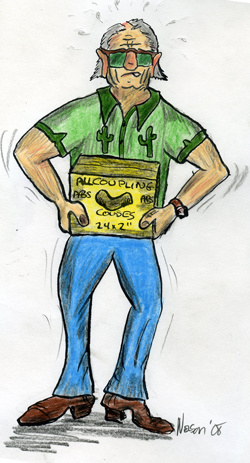
\includegraphics[height=60mm]{corps/chapitre5/img/jerome.jpg}
\end{floatingfigure}

Observant leurs effusions, Romain se souvient qu’à l’époque où Dubé travaillait avec lui comme assistant, la Maririou ne le détestait pas. Loin de là. N’eut été leur grande différence d’âge, elle se le serait peut-être offert. Mais encore eut-il fallut qu’elle soit plus chaleureuse qu’un frigo à bière. Malgré cela, allez savoir pourquoi, quand Romain amenait son jeune collègue à la maison, il fallait la voir se tordre le croupion comme une chatte en chaleur. Fantasme refoulé ?

Que peut donc lui vouloir ce petit malin à l’œil sournois, surtout que voilà bien neuf ans qu’il ne s’est pas pointé. Depuis la retraite du vieux camionneur.

- T’es-tu perdu, mon jeune ? qu’il lui fait en s’approchant.

- Rendu à mon âge, c’est toujours agréable de se faire traiter de «jeune» ! Comment ça va Romain ? Maudit que je suis content de te voir.

Il faudra une solide demi-heure de banalités avant que, cannette de bière en main, l’on passe au vif du sujet. Ce que voyant, Marie retourne à ses confitures en gardant, bien entendu, les deux oreilles grandes ouvertes. Ce qu’elle comprend, c’est que son beau Jérôme se cherche un chauffeur expérimenté pour un travail particulier et que c’est très payant. Extraordinairement payant.

- Je te parle de trois voyages non-stop, back-to-back, Sept-Îles – Toronto. Et au bout, il y a 150 000 \$ qui t’attendent.

Dans sa tête, la vieille dame traduit par «trois aller-retour collés», un périple sans doute fatigant, mais très bien payé. Et un périple probablement risqué. Sinon ça ne serait pas payé à ce tarif. Tout un montant. De quoi s’assurer une meilleure vieillesse. Mais encore faut-il que Romain accepte. Et rien n’indique qu’il va le faire.

- Je suis pas sûr que j’ai envie de rembarquer dans la gamique. C’est pour les jeunes, ça, pas pour un vieux comme moi. J’ai 75 ans et si je me fais attraper, je vais finir mes jours en prison. Ça ne me tente pas. J’ai encore de belles années devant moi, pas des masses, mais quelques-unes, et je n’ai pas envie de les perdre.

Dubé connaît assez Romain pour ne pas insister outre mesure.

- Je te donne mon numéro. Appelle-moi demain dans la journée pour me dire ce que tu décides. Si tu veux vraiment pas, je vais comprendre, mais va me falloir demander à un autre.

Et le gars de s’en retourner dans sa camionnette sous les aboiements.

- Vas-tu te taire, Gros-Prince, pis toi aussi Bedette !

Lorsque, deux heures plus tard, il commence à entrer quelques grands paniers de cerises pour entreprendre leur équeutage, sa conjointe des 47 dernières années l’attaque de front. Elle a toujours fonctionné ainsi, pour son plus grand bien et son plus grand malheur. Elle veut ces 150 000 \$. Et elle les aura, dut-elle conduire elle-même de Sept-Îles à Toronto. De plus, Jérôme est très gentil de «nous» offrir un tel cadeau. Il «nous» fait une fleur. Ça, sur «nos» vieux jours.

- Justement ! Ton Jérôme, je n’ai jamais vraiment pu le piffer. Il a des yeux de rat. Y est pas franc du col. J’ai jamais su ce qu’il pensait !

- Mais voyons ! C’est le meilleur garçon du monde ! Toujours prêt à rendre service !

Fantasme refoulé ?

Et ce fut ainsi jusqu’au lit conjugal. La seule chose qui ne fut pas dite, mais que les deux vieux comprenaient parfaitement bien, c’était que Romain était jaloux de Jérôme, qu’il lui en voulait pour les jeux de croupe de la Maririou. Tant et si bien qu’au matin, tandis qu’il trempait un quignon de pain de ménage dans de la confiture aux cerises fraîche de la veille, il déclara que la nuit avait porté conseil et qu’il téléphonerait à Dubé pour «ramasser le contrat». Marie avait gagné !

Dans un bar de Rimouski, Jérôme lui expliqua l’affaire. Au nord de Matamek, pas trop loin de la Moisie, un hydravion larguerait quelques contenants.

- Je te parle de 90 kilos de coke pure, toute bien paquetée en briques d’un kilo, une valeur de 9 millions sur le marché.

Lui, Jérôme, irait les chercher, ce qui n’était pas de la tarte, et amènerait le tout chez lui, à Sept-Îles, où il préparait trois caisses de 30 briques chacune. Ensuite, il chargerait sa propre camionnette de boîtes toutes semblables, des contenants de coudes en ABS utilisés en plomberie. Mais au travers, il en dissimulerait un plein de cocaïne, lequel serait marqué d’un petit X rouge. Une fois la livraison faite à Toronto, on recommencerait pour le deuxième, puis pour le troisième.

- Pourquoi rien qu’un à la fois, pourquoi trois voyages, pourquoi pas trois gars ?

Jérôme avait expliqué que ses employeurs ne voulaient pas courir de risque.

- Si tu te fais ramasser, ils ne vont perdre que le tiers de leur stock. Pis pourquoi pas trois chauffeurs avec trois camions ? Parce que moins y a de monde dans l’affaire, mieux c’est.

- Ouin ! Mais pourquoi ta camionnette personnelle ?

- Parce que de nos jours, avec les nouvelles plaques électroniques et les GPS, y a plus personne qui veut prendre la route avec un camion volé. On ne ferait pas deux kilomètres avant de se faire barrer le chemin par la police.

Les explications n’avaient pas entièrement convaincu Romain.

Mais pour le versement des 150 000 \$ promis, Jérôme s’était montré plus volubile et lui avait dévoilé la toute dernière technique de blanchiment d’argent. Même si, à cette époque, l’imminent réseau des CRG n’était pas encore en place, il était devenu normal qu’un retraité fasse session notariée de ses biens et devienne ainsi pensionnaire dans un centre d’hébergement privé ou parapublic. C’était selon sa capacité mensuelle de payer. D’où la combine.

Comme tous les bandits n’étaient pas assassinés à 25 ans dans un stationnement de Toronto et que certains atteignaient l’âge de la retraite, les criminels avaient imaginé offrir aux vieux malfrats, une rente annuelle variant entre cinq et vingt mille dollars, une rente tirée sur une banque antillaise. En échange, avait soutenu le verbomoteur Jérôme, ils devaient ne pas poser de question sur un compte qu’on y ouvrait à leur nom «pendant quelque temps». Un gros compte ! Ils devaient aussi signer, les yeux fermés, le testament qu’on leur avait préparé. Ainsi, quand une organisation structurait une opération où il faudrait gratifier des intervenants, elle déposait dans un des ces comptes, tout l’argent nécessaire au soutien logistique, de l’argent qui se retrouverait ainsi nettoyé. Une fois l’opération terminée, on faisait prendre sa retraite au prête-nom et on entreprenait de lui verser fidèlement tous les mois, sa petite rente. Fini les soucis !

- Ça veut dire, mon Romain, qu’il y a quelque part au Canada, un bonhomme qui va bientôt te désigner dans son testament comme étant son héritier pour un montant de 150 000 \$. Autrement dit, un mois ou deux après ta troisième livraison, pas plus, tu vas recevoir la copie légale d’un testament accompagné d’un chèque notarié de 150 000 \$, un beau chèque entièrement légal que tu vas pouvoir déposer dans ton compte.

Une histoire comme celle-là, ça ne s’inventait pas. De toute façon, Romain n’était pas né de la dernière pluie et il avait pris certaines précautions.

C’est ainsi que le lundi suivant, après une courte envolée Mont-Joli – Sept-Îles, Romain se présenta sur l’heure du midi chez son ancien assistant. Il se fit alors expliquer le trajet, le détail bien précis pour se rendre à l’entrepôt de Mississauga en banlieue de la Ville reine, ainsi que les noms des deux gars qui l’y recevraient.

- Y a une petite formalité avant que tu décolles, fit-il en ramassant un canif et une roulette de papier collant, viens avec moi.

La camionnette était stationnée devant la maison et Romain remarqua qu’elle avait la caisse arrière emplie de boîtes en carton identifiées à de la tuyauterie ABS. Son hôte lui fit signe de grimper avec lui et, en petit bonhomme sur le chargement, il déplaça deux boîtes pour être en mesure d’en soulever une troisième dont il coupa le scellant et ouvrit les deux rabats du dessus. Une fois le revêtement de plastique foncé dégagé, il fut possible d’entrevoir les briques du dessus.

- À c’t’heure, fouille dedans et sors en une au hasard. On va l’ouvrir et tu vas y tremper le bout de ton doigt pour y goûter. Comme ça, tu sauras ce que tu transportes.

- Si c’est de la mélamine à Chinois ?

- On verra bien ! Faut que tu saches ! Ils sont comme ça, mes clients !

Après s’être exécuté, Romain grimaça un début de sourire.

- Y a des goûts qui se perdent pas !

Le plus sérieusement du monde, le vieil homme sortit de sa poche un petit trousseau de clés sur lequel était accroché un cube noir de la taille d’un dé à jouer.

- Ça ramasse 600 mégapixels, c’est capable de capter un concert, ça se connecte partout, ça fait tout et ça coûte des pinottes. Là, ça va me servir à filmer la plus grosse quantité de poudre que j’ai jamais vue de ma vie ! J’ai hâte de montrer ça à Marie !

- Pas de danger de me voir la bette ?

- Non non, je ne prends que la boîte.

Une fois le souvenir capté, Jérôme referma le blanc pavée avec soin, le replaça, remit le plastique, recolla les deux battants et déposa les boîtes à leur place. Puis, les deux hommes revinrent sur le trottoir et, côte à côte, s’appuyèrent sur le côté de la caisse de la camionnette. On aurait dit deux copains parlant du dernier match de soccer.

- As-tu vu le X rouge sur la boîte ?

- Je l’ai photographié dans ma tête. Il est sur la boîte juste en dessous de celle-là.

- OK. Ça va aller ?

Devant le signe de tête de Romain, il lui tendit les clés du véhicule.

- Monsieur Romain !

C’était Josiane, la sculpturale conjointe de Jérôme qui l’appelait depuis la porte de côté, celle qui donnait sur la cuisine.

- Vous allez pas partir comme ça, venez manger quelque chose, c’est loin Toronto.

- Non merci, j’ai pas une grosse faim.

- Juste une petite pointe de tarte, alors ? Vous pouvez pas me refuser ça, elle est à la chicouté, c’est moi qui l’ai faite.

Le mot chicouté fut décisif.

- Ça fait de siècles que j’ai pas goûté à ça !

Quand le boulevard Laure recommença à s’appeler 138 à la sortie de Sept-Îles, Romain fit passer son moteur en mode électrique. Il n’avait jamais conduit de véhicule équipé d’un de ces nouveaux accumulateurs à haute performance et il ignorait jusqu’où il pourrait se rendre sur une même charge. Jérôme lui avait bien parlé de Tadoussac, une distance de plus de 400 kilomètres, mais il en doutait; il devrait probablement revenir au très onéreux mode diesel. Les faits lui donnèrent raison puisque l’accumulateur indiqua «Empty» un peu passé Forestville, à environ quatre-vingts kilomètres de sa destination.

Arrivé à Tadoussac en fin d’après-midi, il chercha un motel où il pourrait se louer une chambre, ce qui lui donnerait le droit de recharger son système de batterie. Malheureusement, tous les établissements hôteliers affichaient complet. On lui conseilla alors de continuer jusqu’à La Malbaie, 70 kilomètres de l’autre côté du fjord. C’est ainsi que le septuagénaire prit le traversier et fila vers la petite ville touristique.

Mais plus il roulait, plus le sentiment que quelque chose clochait grandissait en lui. Au départ, les explications au sujet des trois voyages ne l’avaient pas satisfait. Ensuite, si le 150 000 \$ promis étaient bien réels, pourquoi Jérôme, propriétaire de la camionnette, ne les faisait pas lui-même, ces voyages vers Mississauga ? Pour une telle somme, Romain aurait pu rouler jusqu’à la Terre de Feu! Puis, cette histoire de tarte à la chicouté le turlupinait. Voilà une belle fille, Josiane, à l’accent montréalais qui n’avait absolument rien d’une personne capable de préparer des tartes à la chicouté ou à n’importe quoi. Elle l’avait sûrement achetée, sa tarte, laquelle, de toute façon, goûtait la pâtisserie «achetée faite». Si tel était le cas, pourquoi avoir prétendu l’avoir faite elle-même ?

À La Malbaie, Romain aperçut un resto-pompe UltraTard, le fleuron local d’une chaîne de casse-croûte pas trop santé ouverts 24 heures, où il était possible de troquer ses batteries mortes contre des rechargées, de faire le plein en diesel ou, quand il y en avait, en essence ordinaire. Il s’approcha d’une pompe, inséra le pistolet et, même si son réservoir était loin d’être vide, commença son ravitaillement, les coudes appuyés sur la caisse arrière de la camionnette, ce qui lui permettait de voir tout son chargement. Il s’aperçut ainsi que les boîtes du dessus avaient glissé légèrement, ce qui laissait paraître, quelque peu, celles d’en dessous, incluant celle ornée d’un X rouge. C’est à ce moment qu’il eut la certitude d’avoir été floué. Appuyé sur la camionnette du côté conducteur, il n’aurait pas dû être capable de voir le X, lequel n’était visible que du côté passager, comme il avait pu constater en procédant aux vérifications à Sept-Îles. Ou bien on avait ajouté un deuxième X, ou bien la précieuse boîte avait été manipulée.

Le goût de la tarte à la chicouté lui revint !

- J’ai été eu !

Il grimpa dans la caisse, dégagea la boîte marquée et l’ouvrit. Elle ne contenait que de la poussière de pierre. C’est plus qu’il n’en fallait pour que son cerveau soit mis en mode «alerte rouge». Des malfaiteurs l’attendaient à Mississauga avec trente kilos de cocaïne. Or, il ne les avait plus. Cela parce qu’au moment où Josiane lui avait servi sa foutue pointe de tarte, Jérôme avait remplacé la boîte de coke par celle-ci.

Conclusion, Jérôme avait volé ses employeurs et il entendait lui faire porter le chapeau. Or, les méchants ne croiraient pas un seul mot de l’histoire que Romain leur raconterait, cela s’il était assez idiot pour continuer son périple jusqu’à Mississauga. Et, tant qu’à patauger dans la crosse, se pouvait-il que le salopard ait rapporté le vol de sa camionnette pour que les flics ne l’arrêtent ? Non, car il fallait qu’il roule jusqu’à Mississauga pour que les propriétaires de la poudre, des gens qui n’étaient sûrement pas dans un entrepôt de la Maple Leaf City, mais possiblement dans un bureau de la métropole québécoise, le croient coupable du vol.

Sans perdre un instant, il alla payer son diesel et conduisit son véhicule, comme si de rien n’était, vers le stationnement du terminus Intercar, deux coins de rue plus loin. Le tableau de bord étant muni de ressources téléphoniques, il fouina dans sa poche – il n’était pas bête – et il appela Jérôme.

- Y a un problème, lui dit-il d’entrée de jeu.

- Ah oui ?

- Tu m’as changé ma caisse de poudre pour une caisse bidon. J’arrête le contrat, p’is je descends à Sept-Îles te casser la gueule.

- Non non, fais pas ça. Faut vraiment que tu continues jusqu’à Toronto. Tu te trouves à agir comme leurre. Je n’ai pas le droit d’en parler, mais c’est comme ça. La bonne boîte de poudre est ailleurs. Mes employeurs craignent que les flics soient au courant et ils m’ont demandé d’arranger ça de même.

- Ah ouin ?

- Si tu te fais arrêter, ils trouveront rien et ils devront te relâcher. Par contre, pour les deux autres voyages, ça sera différent. Écoute faut que j’te laisse; j’ai ton «collègue» sur l’autre canal. Je te rappelle plus tard ! Bye !

Vraiment n’importe quoi ! Ce Jérôme Dubé le prenait pour un demeuré. Si ces détails étaient vrais, les donner, comme ça, au téléphone, relevait de la pire inconscience. Romain ramassa ses effets personnels, verrouilla la cabine et grimpa dans le dernier bus pour Québec, celui de 21h15, une nouveauté chez Intercar qu’affriandaient particulièrement les touristes gastronomes de la Vieille Capitale. Cependant, avant d’abandonner le camion, il se livra à une petite formalité, une minipolice d’assurance, au cas où !
Une fois à Québec, il prit le car de minuit 45 en direction de Rimouski et essaya de dormir.

Mais au même moment, Jérôme Dubé était sur le bord de la crise de nerfs.

Après sa petite manipulation pendant que Romain goûtait à la tarte de Josiane, il avait placé la boîte de 30 kilos, la seule et vraie boîte de cocaïne - les deux autres n’étant que billevesées imaginées pour mieux enfirouaper Romain - dans la section arrière de son automobile, une hybride trois portes très économique louée l’hiver dernier au moment où le prix du litre avait basculé à plus de 6 \$. Il savait pouvoir se rendre jusqu’à Tadoussac avec ses batteries chargées à bloc; il l’avait déjà fait. Au pire, il savait qu’il pourrait s’accommoder à Forestville; il connaissait un motel où il pourrait refaire sa charge tout en s’offrant une bonne nuit de sommeil.

De toute façon, il n’était pas pressé. Il avait tout son temps pour se présenter chez les deux Portugais près du parc Jeanne-Mance à Montréal, des gens qui ne semblaient pas craindre l’ire des vrais propriétaires de la coke, des hommes d’affaires au-dessus de tout soupçon qui avaient pignon sur rue à moins d’une heure de route plus au nord. Comme la qualité de son produit était excellente, le Septilien escomptait pouvoir en obtenir au moins un million et demi de dollars US versés dans un compte antillais ouvert à son nom.

À 16 h, il prenait la route, réalisant, au fur et à mesure qu’il les croisait, que toutes les stations d’essence n’avaient plus que du diesel. Mais, bon, il n’était pas inquiet, connaissant l’autonomie énergétique de son bolide. Le cœur en fête, il n’arrêta même pas à Baie-Comeau et traversa le pont de la Manic en rêvant de la dolce vita qui l’attendait dans les Caraïbes.

Pourtant, à quelques kilomètres de Ragueneau, la circulation commença à s’alourdir. Plus il approchait du village, moins il avançait. La 138 était bloquée. Jérôme se retrouvait prisonnier dans un convoi de véhicules long à ne plus finir, essentiellement des camions. De temps à autre, on avançait de quelques mètres. On aurait dit une meute affamée de gastéropodes flairant des laitues bien fraîches.

Il eut l’idée de syntoniser le canal d’urgence où il apprit que la 138 était temporairement fermée, un forcené s’étant barricadé dans sa maison avec des otages. On avait détourné la circulation dans un chemin de bois plus au nord, une route du siècle dernier qu’on n’avait pas conçue pour recevoir autant de fardiers. Tant et si bien que les plus lourds en arrachaient, peinaient et s’enlisaient. Rien n’allait plus.

C’est ainsi que Jérôme mit près de trois heures pour contourner le village en calant parfois jusqu’aux essieux. Eut-il dû faire volte-face et retourner à Baie-Comeau ? Oui, si on en croit les événements à venir. Car il s’aperçut que son système d’accumulation était presque épuisé. En fait, il ne lui restait même plus assez d’énergie pour atteindre Forestville, 50 kilomètres plus loin. Pire, le seul endroit où on aurait pu lui échanger ses batteries vides était fermé.

Mais la chance lui sourit au sortir du village quand il aperçut le placard tout illuminé du «Motel de la Forêt». Seul gîte du secteur, l’établissement semblait disposer de quelques bornes de chargement électrique non assignées. À l’officine d’accueil, un employé lui en désigna une tout près de la route, juste sous l’énorme enseigne. Jaugeant l’état général de délabrement du commerce, le voyageur préféra ne pas louer de chambre et s’en tenir au gavage de ses batteries. De toute façon, puisqu’une recharge complète ne prenait que deux heures avec les nouveaux accumulateurs, il calcula pouvoir reprendre la route à minuit et arriver à son hôtel de Tadoussac une heure plus tard. Ce qui n’était pas si mal.

Son auto branchée à la borne, Jérôme abaissa son dossier et s’écrasa confortablement en écoutant de la musique Motown. Au bout d’une demi-heure, la faim commença à l’incommoder; il n’avait rien mangé depuis le midi. Et encore ! Il n’avait avalé qu’une pointe de tarte à la chicouté accompagnée d’un verre de lait. Il eut l’idée d’aller à l’accueil se chercher des cochonneries, ce qui lui couperait la faim jusqu’à son arrivée à Tadoussac. Ce qu’il fit !

Malheureusement pour lui, deux paires d’yeux l’observaient depuis les fourrés. C’étaient deux jeunes Innus un peu paumés.

- Tshika ui shassikutshiakanu, tshe itinamuat mukumanu ushkutit. Tshek eka minupaniti, tshe tshitishimuiaku minashkuat, dit le plus vieux des deux, ce qui pourrait se traduire par : «On arrive à la course, tu lui pointes ton couteau sur le nez» (pour ne pas nuire à la compréhension du récit, nous allons continuer en français).

- Ouin.

- On l’oblige à sortir du char, on saute dedans et on se sauve. Ça marche ?

Le plus jeune n’avait pas l’air convaincu.

- D’in coup qu’i se défend ?

- On se pousse dans la nature !

- Ouin, j’sais pas …

- T’aimes-tu mieux marcher 25 kilomètres ? Moi pas !

Au même moment, Jérôme se glissa hors de sa voiture pour s’en aller à l’accueil.

- Attends, dit le plus vieux. Il s’en va au Motel. Es-tu capable de voir s’il a laissé ses clés ?

L’autre malvat s’approcha silencieusement et fit un signe affirmatif de la tête.

Cinq secondes plus tard, les deux gredins étaient assis dans la voiture, après l’avoir déharnachée de sa borne, et avaient mis le contact. Le plus vite qu’ils le purent, ils foncèrent sur la 138 et disparurent en direction de Betsiamites, une communauté établie en bordure du fleuve entre Ragueneau et Forestville.

Jérôme fut tellement ahuri par ce qu’il venait de voir que la bouche lui resta grande ouverte. Des gens venaient de fuir avec son million et demi de dollars US en belle poudre blanche ! Des gens qu’il ne connaissait pas, cela, le soir tard, dans un coin perdu où il n’avait aucun contact. L’employé du motel qui avait tout vu, accouru.

- Je les ai reconnus. Pas des méchants gars. D’habitude, ils font pas ça. Faut croire qu’ils étaient cassés. Ils s’en vont à Betsiamites avec ton char.

- Betsiamites, sur la Réserve ?

- C’est ça qu’i faut dire aux flics. Mais ça donnera rien. Comme d’habitude, ils vont attendre à demain et là, ils vont téléphoner à la police amérindienne. Surtout à soir; ils sont tous occupés avec le fou qui s’est barricadé. C’est sûr que ça va aller à demain. Et là, si ton char a pas été mis en morceaux, ils vont peut-être le trouver et te le ramener. Sinon, fais-en ton deuil !

Pour Jérôme, la cause fut vite entendue. Si les autorités retrouvaient l’auto dans les minutes suivant l’appel comme c’était souvent la pratique avec les technologies GPS, ils s’intéresseraient sûrement à la caisse de coudes en ABS marquée d’un X rouge. Ils sont comme ça, les flics. En revanche, s’ils n’entreprenaient les procédures que le demain, il est fort probable que les voleurs auraient ouvert la boîte et se seraient occupés de son contenu. Auquel cas, elle ne serait plus dans l’auto quand la police la retrouverait. Advenant qu’ils y arrivent, bien sûr. À ce moment, il n’y aurait plus de danger pour lui. Conclusion, il semblait plus prudent de rapporter le vol. Ce faisant, Jérôme se donnait même du temps pour fuir advenant qu’il doive le faire.

- J’ai plus rien pour téléphoner, c’était dans mon auto …

L’employé, un solide gaillard dans la trentaine, lui fit un signe de la main.

- Viens en dedans, on va t’arranger ça.

Dans la demi-heure qui suivit, Jérôme s’était fait aviser, tel que prévu, qu’en raison des événements, toutes les forces policières disponibles avaient été affectées au village et qu’ils communiqueraient, dès demain, avec leurs confrères de Betsiamites. Puis, la belle Josiane, la dame aux tartes achetées faites, lui avait promis qu’elle viendrait le prendre à Ragueneau, à l’autre bout du village, «pour ne pas être pognée dans le barrage routier», dans trois heures. En état de choc, ne pensant qu’à son million et demi et se sentant littéralement impuissant, l’ex-assistant de Romain Tardif dit le Gelé, avait accepté une bière de consolation et avait commencé à tuer le temps.

- Si j’y vas, là-bas, ça peux-tu donner des résultats ?

- Où, à Betsiamites ? À soir ?

- Oui

- Tu vas te faire casser la gueule. En plus de ne plus avoir de char, t’auras plus de dents.

- Je sais me défendre…

- Moi aussi, mais moi, je resterais ici bien tranquille.

Dubé n’avait pas été convaincu.

- Je te l’ai dit. Ce n’est pas du mauvais monde; ils vont probablement laisser ton char à un kilomètre de la réserve et finir à pied, ni vu ni connu. Ce sont pas des voleurs. Juste des jeunes sur le party.
Au même moment, les deux délinquants stationnaient la voiture devant une des maisons face à la plage. Assis sur sa galerie en train d’observer les reflets de la lune sur le fleuve, Joseph Picard les aperçut et leur fit signe. Depuis une dizaine d’années, l’homme était fortement impliqué dans une mécanique de redécouverte et de réappropriation de l’esprit innu, de la langue et des traditions, un long processus de redressement moral, de revalorisation sociale et de cheminement vers une fierté ethnique de bon aloi. Il questionna les deux gamins et quand il comprit, il ne put s’empêcher de les coiffer d’épithètes plutôt désagréables.

- Un Blanc qui vole un char, c’est rien, c’est juste un cave. Un Innu qui le fait, c’est un asti d’Indien. Pire, un Indien saoul ! Un Indien crotté ! Un Indien drogué ! C’est ça que vous voulez entendre quand la police va venir vous ramasser ?

Joseph s’approcha du véhicule et en fit le tour.

- C’est à qui ?

- À un Blanc qui s’était arrêté au premier motel à Ragueneau.

- C’est quoi la boîte en arrière ?

Les deux jeunes haussèrent les épaules.

Pris d’un doute, l’homme ouvrit le hayon et avec son couteau de poche, décacheta la boîte. Il ne lui fallut qu’un instant pour tout comprendre. Vivement, il fouilla dans ses poches, prit son trousseau de clés et le lança au plus vieux des deux noceurs.

- Toi, tu vas en arrière de la maison, tu ramasses un pic, une pelle et le cinq gallons d’essence sur la galerie, tu prends mon pick-up et tu me suis. Toi, le jeune, tu montes avec moi. Y a pas une minute à perdre.

- C’est quoi l’affaire ? demande celui-ci tandis que l’autre disparaît.

- L’affaire ? Vous vous êtes mis dans la marde. Le char que vous avez volé, il appartient à la grosse gamique. Tu veux-tu que son propriétaire à la boîte, il vienne ici la chercher ? Tu sais-tu ce qu’il y a dedans, la boîte ? Des kilos de coke ! C’te boîte-là, c’est la mort, la mort blanche, notre mort !

Cinq minutes plus tard, en plein bois, sur une route qu’on aurait dit conçue pour des VTT, l’auto électrique s’arrêta en panne sèche, façon de parler. Heureusement, Joseph avait une chaîne dans la caisse de sa camionnette. La voiture du Septilien Jérôme Dubé fut ainsi remorquée jusqu’à sa destination finale, un trou que les deux jeunes durent creuser, piquer, bêcher et pelleter pendant plus d’une heure, parce qu’il n’était pas assez creux. Ils y placèrent l’auto, Joseph l’enduisit d’essence et il l’enflamma. Puis, doucement, la tête vers le sol et les yeux fermés, il prit les mains tout endolories des deux malheureux.

- Ce qui brûle dans ce trou, c’est le mauvais en nous. Le mauvais qui sort, qui sort, qui s’en va dans les flammes. Dans le feu avec la mort blanche qui se brûle elle-même. Et le mauvais qui s’en va, il se trouve à laisser de la place, un vide. Un vide à côté du cœur, un vide à côté de l’esprit. Et un vide, ça peut pas rester vide. Faut que ça se remplisse. C’est la loi de la Terre. Et on a quoi pour le remplir le vide ? Seulement du bien, du bien qu’on va essayer de faire, du bien qu’on va générer, du bien qui appelle le bien, du bien pour nous, pour notre communauté, pour nos jeunes, nos aînés.

Dans la violence des flammes et de leur crépitement, un silence humain suivit.

- Bon, faut finir la job, à c’t heure ! finit par dire le mentor. Vous voyez le tas de roches ici à côté ?

- C’est des roches qui ont servi à des meteshun, fit le plus jeune, grand amateur de ces cérémonies de sudation spirituelle.

- C’est pas grave. Vous allez les placer sur l’auto pour bien la cacher. Faut que rien ne paraisse.
Personne ne devra savoir qu’en d’sour, y a un char et une boîte de mort au rat qu’on a fait brûler.

Il fallut encore une heure aux deux jeunes pour que le tas de pierres, des roches de la grosseur de gros pamplemousses, soit complètement déplacé sur la carcasse fumante. Au matin, les trois Innus revinrent avec des râteaux et quand ils eurent terminé leur nettoyage, plus rien de compromettant ne pouvait désormais attirer l’attention. De toute façon, d’ici l’hiver, la nature aurait parfaitement complété la dissimulation finale aussi bien d’une voiture neuve que d’une caisse terriblement létale.

Mais à Sept-Îles, Jérôme était sur le bord de la crise de nerfs.

Depuis son retour, vers 7 h, il tournait en rond, incapable de se concentrer sur la marche à suivre. Les ennuis s’accumulaient. À peine avait-il eu le temps d’arriver qu’un enquêteur de La Malbaie l’avait joint au téléphone. Il venait d’attraper les deux voyous qui avaient volé le chargement de coudes en ABS, un «chargement offert au grand jour» dans la caisse de la camionnette dont il était le propriétaire, un «véhicule oublié» au terminus d’autocars.

- Si vous pouviez passer d’ici 24 heures pour faire votre déposition et signer une pile haute comme ça se paperasse, ça ferait bien mon affaire.

- Oui, je m’en occupe.

- Juste comme ça, en passant. Pourquoi avez-vous laissé votre camionnette pleine de marchandise qui coûte cher, ici à La Malbaie ? Sur mon logiciel, je vois que vous êtes présentement à Sept-Îles. Vous êtes redescendu comment ?

Jérôme avait dû improviser rapidement.

- C’est une histoire de chicane avec ma conjointe. Elle est partie hier avec mon camion sur un coup de tête et, rendue à La Malbaie, elle a choisi de continuer en autobus.

- Une chicane d’amoureux.

- C’est ça.

- Votre conjointe a été filmée en train de faire le plein à l’UltraTard d’à côté et de descendre de votre véhicule au terminus d’autocars. Elle a même été filmée en train de s’acheter un billet pour la ville.

Le cœur de Jérôme avait cessé de battre.

- En venant faire votre déposition d’ici 24 heures, Monsieur Dubé, allez-vous avoir la gentillesse de m’expliquer pourquoi votre conjointe ressemble à un retraité à moustache portant une queue de cheval de l’ancien temps ? Et, tant qu’à me gratifier de vos bontés, allez-vous pouvoir m’expliquer le lien, si lien il y a, bien entendu, avec le vol de voiture que vous avez rapporté hier soir à Ragueneau ?

L’horreur n’avait plus de nom. Il ne lui restait plus d’autre choix que de filer et le plus tôt serait le mieux. Ainsi, Romain n’avait pas cru à son histoire de leurre et avait abandonné la camionnette à La Malbaie. Puis il avait pris l’autobus, probablement pour revenir chez lui. Ce n’était plus qu’une question d’heures avant qu’il ne rapplique ici avec un bâton de baseball.

- Sacrament !

Tout avait foiré. Les flics l’avaient dans leur collimateur, les Indiens avaient piqué la coke et Romain s’en venait lui casser la gueule. Il ne lui restait plus qu’une carte à jouer, ses «employeurs» du Nord de Montréal. Il leur dirait que le messager, un certain Romain Tardif que Josiane avait filmé en train d’inspecter son chargement et goûter à la poudre, laquelle on apercevait très bien sur le document, avait préféré livrer la marchandise aux Indiens de Betsiamites et qu’il était disparu avec l’argent. Il ajouterait que lui, Jérôme, il le recherchait partout et que s’il le trouvait, il lui ferait tout cracher. Comment il savait pour Betsiamites ? C’est que la puce de traçabilité placée dans la caisse avait cessé de fonctionner en plein milieu de la réserve.

Ce qu’il fit, en omettant toutefois de parler des Indiens et de Betsiamites, avant de se payer un aller simple sur le vol de l’après-midi Sept-îles-Montréal.

- C’est Josiane qui va être fâchée, dit-il en bouclant sa ceinture.

Au même moment, de l’autre côté du fleuve, Romain s’installait avec sa Maririou dans le chantier de Timothée sur la rue Crouet. À son arrivée à Saint-Anaclet, au petit matin, il était entré chez lui en criant au branle-bas de combat. Fallait se dépêcher, tout avait «chié», la combine n’était qu’une «crosse» pour que Jérôme fasse une «grosse passe», les «gars de la dope» avaient leur adresse ici à Saint-Anaclet, ils voudraient récupérer leur bien, ils étaient probablement déjà en route, il n’y avait plus une minute à perdre.

- Mais j’ai quand même une carte d’atout !

Romain le Gelé n’avait pas voulu en dire davantage. En une demi-heure, les deux vieux avaient empli leur voiture de tout ce qui, à leurs yeux, pouvait avoir de la valeur: papiers, partitions, instruments de musique, souvenirs, nourriture, quanticordi et un chiot laid comme les sept péchés capitaux que la Maririou appelait Gazou. Puis, ils avaient pris la poudre d’escampette. «La pédale au fond !» C’est la vieille qui appela Timothée pour qu’il les attende avant de partir pour son travail au ministère de la Santé. Mais c’est le bonhomme qui rappela pour annuler la consigne et pour, plutôt, lui donner rendez-vous dans un resto de Rimouski-Est.

Là, un plan d’action fut mis au point. On stationna d’abord l’automobile de Romain derrière l’édifice du ministère où Timothée officiait en tant qu’agent classe IV. Puis à coups de petits voyages discrets qui durèrent toute la journée, on transborda les effets personnels des deux vieux, lesquels dès le premier voyage, disparurent à tout jamais dans un sous-sol en pleine rénovation. Cet aspect du casse-tête réglé, Timothée abandonna la voiture de son père dans un rang sans surveillance sur les hauteurs de Rimouski et revint à pied. Il dut marcher pendant plus de trois heures.

Le lendemain matin, la télévision leur apprit que pendant la nuit, la fermette des Tardif, à Saint-Anaclet, avait été entièrement rasée par les flammes, un incendie probablement criminel, compte tenu de son extrême violence. Le corps des occupants, Romain Tardif et sa conjointe Marie Rioux, n’avaient pas été retrouvés dans les décombres, mais, fait navrant, les restes calcinés de deux grands chiens l’avaient été. Quant aux animaux de ferme, essentiellement de la volaille, quelques chèvres et des lapins, ils avaient tous été massacrés. Par ailleurs, la voiture du couple avait été retrouvée abandonnée sur le chemin d’un rang voisin. Enfin, disait-on, les enquêteurs étaient à la recherche de pistes et tout renseignement pouvant les aider était le bienvenu.

- Bedette, Gros Prince !

Romain avait pleuré, sans que la Maririou, le regard plus dur que jamais, n’arrive à lui mettre la main sur l’épaule.

Ainsi débuta la vie recluse du couple Tardif-Rioux. Pendant les premiers mois, les ajustements furent difficiles. Il fallut terminer les rénovations, cela sans revenus aucuns, l’État les considérant comme disparus ou décédés et leur compte en banque ayant été gelé par les autorités judiciaires. Il fallut également s’adapter à la promiscuité inhérente au petit logement du sous-sol. Mais le pire, c’est qu’il fallut se faire à l’idée que jamais plus ils ne pourraient aller profiter à leur goût du grand air.

\begin{floatingfigure}[l]{40mm}
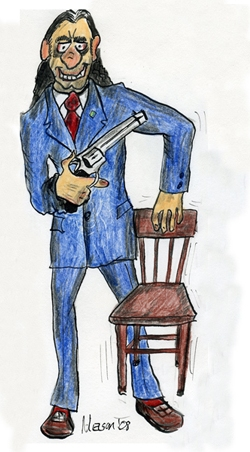
\includegraphics[height=60mm]{corps/chapitre5/img/alessandro.jpg}
\end{floatingfigure}

Le 8 février suivant, c’était un mardi en fin d’après-midi, le trio s’apprêtait à répéter une pièce, des pas se firent entendre dans l’escalier. Seul Gazou se montra hostile, prêt à l’attaque; les autres furent pétrifiés. Un homme habillé en président de compagnie et chaussé de pompes italiennes à 1 000 \$ pénétra dans la pièce et, d’un geste de la main, celle qui tenait le Smith \& Wesson modèle 500 à cartouches Magnum, fit comprendre à la Maririou qu’elle avait intérêt à policer sa bête.

- Gazou, ici, viens voir Maman !

À l’époque, elle n’avait pas encore commencé à chuinter.

Puis, de son canon, l’homme fit signe à Timothée de lui céder sa chaise.

- Je détesterais vous déranger trop longtemps, dit-il. Alors, je vais faire vite. Permettez-moi de me présenter, Alessandro Costi, homme de main. Mon travail, dans la vie, consiste à passer en arrière de crétins que mes clients utilisent bêtement quand ils veulent communiquer des messages. Moi, je ne mets jamais le feu et je n’égorge jamais de poules. Je me sers plutôt de ma tête. Par exemple, quand je cherche des gens qui n’ont pas laissé de traces et qui ne dépensent pas des fortunes dans des endroits extravagants, je regarde s’ils ont de la famille, ce qui est souvent facilité par les médias où on interview les enfants éplorés de parents dont les corps ont disparu. Et quand, de cette façon, je découvre un fils et que je m’aperçois qu’il achète de la bouffe pour trois, de la nourriture épouvantable, soit dit en passant, et du linge de femme dans des friperies, je me mets à suivre cet imbécile jusqu’à son terrier. Et là, bello caso, je descends les marches et devinez ce que je trouve ? Le type qui a été engagé pour livrer à mes clients trente kilos de coke mais qui a disparu avec la marchandise.

Personne n’osa parler. Seul Gazou eut le courage, ou la bêtise, de grogner.

- Comme personne ici n’a de temps à perdre, je vais poser la question une fois, une seule fois. Si, au bout de cinq secondes, je n’ai pas eu ma réponse, je tue le chien. Au bout de dix, je tue la madame et au bout de quinze, le fils à son papa, ici. Après, je vais devenir plus subtil. Mon pauvre monsieur, je vais devoir te faire éclater les rotules à coups de cartouches .500, ensuite les oreilles, puis quelques doigts et ainsi de suite, jusqu’à ce que j’aie ma réponse. Je ne pourrai malheureusement arrêter les tourments que si tu parles. Mais avant d’y arriver, si tu t’obstines, ça risque d’être assez long et pénible. Capito ? Alors voici la question : musique, roulements de tambour, gros plan sur le concurrent : où se trouvent les 30 kilos de poudre qui appartiennent à mes clients ?

Doucement, Romain déposa sa clarinette.

- C’est inutile. J’ai ta réponse. J’ai tout ça sur un mini cube numérique multifonction.

- Est-ce que ça nous apprend où est le bien de mes clients ?

- Non mais ça va b’en manque te montrer que je ne l’ai jamais eu et tu vas comprendre qui est parti avec.

Alessandro Costi réfléchit quelques instants.

- Perché no ? Je veux bien jouer le jeu; je ne suis pas à une minute près. Fais voir, mostrami !

Romain s’approcha d’un des rayons de bibliothèque et s’empara de l’édition 2006 du Petit Larousse qu’il ouvrit en son milieu. Un trou y avait été aménagé comme pour servir d’abri au mini-cube. Il le prit et le remit au visiteur.

- Ingegnoso ! Connecte-le à ton ordi, qu’on en profite tous ensemble.

Romain venait de jouer sa carte d’atout. Il avait enregistré l’intégralité de sa conversation avec Dubé dans un bar de Rimouski lorsque son ancien assistant lui avait expliqué le travail, incluant les trois livraisons à Toronto, le paiement de 150 000 \$ par chèque notarié et l’hydravion dans la région de Matamek. Puis ils purent visionner des images de la coke avec, comme fond sonore, les voix de Jérôme («Pas de danger de me voir la bette ?») et de Romain («Non non, je ne prends que la boîte»). Puis ce fut la conversation téléphonique où on lui révélait son rôle de leurre. Enfin, ce fut la scène du stationnement où on pouvait voir que la poudre avait été changée en poussière de pierre.

L’homme des choses interlopes se gratta le crâne avec le canon de son S\&W.

- Porca miseria ! Tu t’es fait boulechitter en grande, Signore Romano.

La Maririou regarda son vieux comme si c’était la première fois qu’elle le voyait, Timothée paru en phase de réanimation et Gazou déposa sa mauvaise tête sur ses petites pattes croches.

- Avec ces éléments nouveaux, il va se passer deux choses, mon bon Monsieur Romain. Moi, je m’en vais essayer de retrouver ton bon ami Jérôme. Amici dei miei amici sono miei amici, comme on dit à Ville-d’Anjou. Vois-tu, j’ai une question à lui poser. Une seule. Toi, Romano mio, tu vas rester ici bien tranquille avec ta femme et ton chien jusqu’à ce que je te fasse signe. Y a des cretinos dans la nature, ceux qui ont mis le feu et qui te cherchent encore. T’as compris ? Ne bouge pas, attend mon signal. Après, tu feras ce que tu veux. Pourquoi je vous élimine pas, toi et ta befana ? Parce que vous êtes trop vieux pour me nuire.

- Euh, et moi ?

- Toi le fils, fais comme d’habitude, mais sois prudent. Ils sont trop cons pour connaître ton existence. Dans ton cas, t’es p’t-être pas trop vieux pour me nuire, mais t’es trop timoroso. C’est ce qui te sauve la vie. On est bien peu de choses, non ? De toute façon, ça ne sera pas bien long avant que je vous fasse signe.

Exactement sept semaines plus tard, le 28 mars, Romain recevait un courriel 3D anonyme où on pointait sur un article de la Cyberpresse relatant la découverte d’un cadavre flottant sous le Pont de Québec. Jérôme Dubé avait été retrouvé.

- Tout un signal, s’était dit le vieil homme.

Mais la journée même, le Gros Turcotte déposait en chambre son projet de Réforme et en octobre suivant, un référendum faisait de Romain et Marie, deux illégaux. Auraient-ils pu, avant de le devenir officiellement, reprendre leurs identités et recommencer à bénéficier des services gouvernementaux ? Toucher des assurances ? Être dédommagés par le Fonds d’aide aux victimes d’activités criminelles ? Pour que cela soit possible, il leur aurait fallu expliquer une très longue histoire à différents corps de police, à différents bureaux de fonctionnaires, avec toutes les conséquences que cela aurait impliquées : procès, emprisonnement, danger de règlement de compte, peur constante, misère noire.

C’est probablement ce jour-là, le 28 mars 2028, qu’ils se résignèrent à finir leurs jours dans un sous-sol de Nazareth. Quant aux 30 kilos de cocaïne, ils ne furent jamais retrouvés. Par contre, Alessandro Costi, lui, il le fut vers la fin juin de la même année. Il marchait en chaussettes sur la 138, à mi-chemin entre Betsiamites et Forestville. Il était hagard. On l’avait dérouillé et dépouillé de sa voiture, de ses chaussures à 1 000 \$, de son Smith \& Wesson Magnum .500 et de son EP (émetteur personnel). Qui lui avait fait subir un tel traitement ? On ne le sut jamais. Par contre, il est permis de conclure qu’avant d’aller flotter sous le Pont de Québec, Jérôme Dubé avait pleurniché autour de l’histoire des deux jeunes de Betsiamites.
\chapitre{Du manger mou aux nouvelles, le mardi 19 juillet 2033}{Trop «timoroso»,}{ avait dit l’inimitable Alessandro Costi. Trop poltron, trop pissou, trop chie-en-culotte ! Il est vrai que Timothée ne s’accordait pas grand mérite du côté bravoure. Quand on passe une partie de sa vie à longer les murs ou à marcher en fixant le trottoir, on n’apprend pas à braver les affreux, à défendre ses pieds carrés, à faire sa place sous le soleil du petit Bon Dieu. On ne devient jamais audacieux au point d’ajouter quatre cordes supplémentaires à sa lyre pour l’imposer aux quatre coins cardinaux. }

On se contente de faire le moins de couacs possible avec un trombone qu’on déteste, qu’on nous a forcé dans la gorge à grands coups de masse. On suit sa partition sans maugréer, après, on essaie de filer sans se faire voir. On refoule quotidiennement l’envie d’envoyer paître l’affreuse mégère qui bat la mesure entre deux cuissons de confiture aux cerises. Timothée de Milet n’a sûrement pas eu de mère. Ou s’il en a eu une, elle est disparue alors qu’il était nourrisson. Assis dans son officine le moral en compote pour cause de souvenirs recensés, le fils de la Maririou ne remarque pas tout de suite la stature massive de Robespierre Alcide qui occupe son cadre de porte.

- À ta question d’hier, j’ai une question.

Timothée lève la tête.

- T’en veux combien ?

Il est direct ce matin, le collègue !

- Euh… deux ? C’est-y compliqué ?

Robespierre lui lance une petite bouteille de Tylenol en le gratifiant d’un clin d’œil.

- Attrape, y en a justement deux là-dedans.

Et il disparaît avant que le CS-1 puisse dire quoi que ce soit, dire quelque chose comme “merci infiniment !”, ou comme “bonne idée d’avoir mis ça dans une bouteille vide de pilules; ça va mieux passer devant les détecteurs d’objets”, ou comme “laisse faire, l’idée me rend insomniaque”, ou comme “en aurais-tu une troisième ?”.

Mais, à bien y penser, comment le gaillard a-t-il su qu’il en fallait deux ? Se douterait-il de quelque chose ? Personne n’est au courant ! Personne ne doit l’être ! Reste que la question est maintenant de savoir comment refiler cette «solution» à ses parents. Comment avoir le courage de le faire. Comment ne pas être «timoroso» ! Y en a-t-il seulement d’autres, de solutions ? Les génératrices à espoir, les matrices à espérance, les dynamos à lumière-au-bout-du-tunnel, étaient toutes tombées en panne depuis belle lurette et Timothée avait été recalé au certificat en technique jovialiste. Depuis que la société, essentiellement faite de brutes grégaires, était devenue folle, folle et impitoyable, plus que jamais, la pilule du bonheur représentait une avenue moralement défendable. Encore fallait-il pouvoir la présenter, la soutenir, l’administrer. Assistance à deux suicides ? Meurtres par compassion avec circonstances atténuantes ? Euthanasie avant l’état grabataire ? L’être humain n’a-t-il pas le droit de décider d’aller voir ailleurs quand il s’emmerde dans une grisaille sans pitié, sans gratifications, sans améliorations possibles ?

- Chiennerie !

Mais pour l’instant, il doit descendre à la cafétéria son tube de Tylenol en poche. Une note de service de Carl Michaud, l’inquiétant directeur général du Centre, lui en a intimé l’obligation. C’est en fait une journée dont le grand patron pourrait se passer. Il lui faut en effet accueillir Ti-Dédé, c’est-à-dire T.I.D.D. ou Thierry-Ian Dennis-Dubeau, le chef des Verts et chef de l’opposition à Québec. Flairant des élections à l’automne, l’homme politique parcourt le Québec en quête de munitions et de plates-formes pour tester quelques ballons d’essai. Son ambition ? Devenir le premier Vert de l’histoire à diriger le Québec. Rien de moins ! 

\begin{floatingfigure}[l]{40mm}
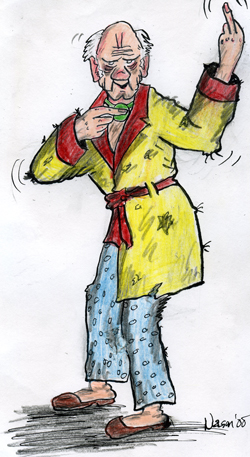
\includegraphics[height=60mm]{corps/chapitre6/img/personnage-vader.jpg}
\end{floatingfigure}

Au moment où Ti-Dédé fait son entrée dans l’établissement, Philippe «Flipper» Dauphin jette un dernier coup d’œil à la cafétéria. Directeur des communications et âme damnée de Carl Michaud, sa mission est de réduire tant qu’il le peut tout potentiel de retombées négatives. Apercevant Dart Vader assis avec les quatre pensionnaires en 2P (salles communautaires pour personnes autonomes) choisis minutieusement par lui-même, Flipper le fait chasser in extremis par ses deux adjoints en uniforme de la Sécu, deux gorilles épouvantables.

- J’ai autant le droit qu’eux autres à être ici, moi, métallise-t-il de sa canule.

Mais rien n’y fait. Les sbires du Flipper l’entraînent vers la sortie. Il faut dire que le sieur Dauphin sait s’entourer. Les horribles frères «Papynut» et «Bluesly» Côté sont habituellement gardés au sous-sol en tant que geôliers. Comme les employés du Centre n’arrivaient pas à les départager, on en était venu à les appeler «PapyBlues». On disait, par exemple, «Je descends chez les PapyBlue !» ou «Penses-tu sérieusement que les PapyBlues s’adonnent à la torture ?» ou «Madame Thériault, si vous n’arrêtez pas de tanner madame Labbée, je vais vous amener chez les PapyBlues !». Avec le temps, les abominables frangins dont les sobriquets remontaient à leur jeunesse de hockeyeurs semi-professionnels avaient appris à ne pas poser de questions, ce qu’ils faisaient très bien.

Grand, distingué, affable, habillé en carte de mode, Ti-Dédé, suivi de son escorte, des patrons du Centre et d’une petite horde de journalistes, serre des mains ici et là au hasard de sa promenade dans les zones autorisées du rez-de-chaussée dont fait partie la cafétéria. Sans surprendre personne, il y entre et s’approche d’une table où quatre bons vieux qu’on a astiqués et mis en scène viennent soi-disant de finir leur ration de Nutrisuz, sourire aux lèvres. Adoptant cet air sérieux que les politiciens doivent afficher quand il faut dénoncer une iniquité, le chef politique fait face aux représentants des médias.

- Mesdames et messieurs les journalistes, je me demandais, en entrant ici, si mon bon ami monsieur Michaud, le souriant directeur général de cet établissement ultra moderne, ne pourrait pas nous faire servir, à chacun d’entre nous, personnel politique, fonctionnaires du MAG ou journalistes, une portion de Nutrisuz, ce brouet que tout le monde, ici, appelle «manger mou». Ainsi, à l’heure où des débats ont cours sur la nature de ce produit et sur ses conséquences sur la santé publique, nous serions plus en mesure de pouvoir nous en faire une opinion. Qu’en pensez-vous, cher ami ?

Carl Michaud avait prévu le coup et fait un signe de tête à Amédée Chicot qui, aidé de Simon Saint-Pierre, passe à l’action. En moins de deux minutes, tous les visiteurs se sont fait remettre par un «bénévole» empathique, un contenant d’ABS chaud empli de Nutrisuz à saveur de fruits de mer à l’ail. Pas si mal pour un petit mardi de semaine au tout début de l’avant-midi !

- Il y a des breuvages disponibles à la fontaine, eau, limonade ou thé, fait remarquer Michaud à voix haute. Demandez à nos sympathiques bénévoles, ils vous fourniront le contenant nécessaire.

Ostensiblement, Dennis-Dubeau n’apprécie pas son plat et, mimiques à l’appui, il semble questionner son entourage où, selon toute vraisemblance, un consensus est en train de s’établir à l’effet que cette nourriture est une honte. Ici et là, des journalistes y trempent le bout des lèvres et se regardent les uns en riant, d’autres en grimaçant. Voilà plus qu’il n’en faut pour que le politicien reprenne la parole.

- Mesdames et messieurs les journalistes, si vous voulez bien me permettre d’interrompre votre succulent repas, je ne serai pas long.

Même si les rires escomptés font défaut, le tribun lève les deux bras.

- Mesdames et messieurs, vous goûtez présentement à cette bouette infâme que nous, la société québécoise porteur de ce flambeau allumé il y a 500 ans par un navigateur breton appelé Jacques Cartier, que nous, dis-je, servons à nos aînés, à ceux-là même, à celles-là mêmes, qui ont façonné le Québec moderne dans lequel nous évoluons tous et toutes. Ce concentré de produits chimiques importés des États-Unis au mépris des quotas de gaz à effet de serre, est une aberration à laquelle nous les Verts, allons nous attaquer dès le lendemain de notre prise du pouvoir, si jamais le premier ministre a le courage, je dis bien le courage, de déclencher des élections ! Nos aînés méritent de manger de la vraie nourriture, pas un résidu de compote électrochimique. Vous croyez que j’exagère ? Que je parle en politicien ? Portez plutôt attention à la liste des éléments de base du cocktail que l’on fait ingurgiter à nos pères et à nos mères.

Il a mis ses lunettes et a ouvert un calepin.

- Je vous traduis ce qu’on peut lire en anglais, et uniquement en anglais, ce qui, soit dit en passant, est un accroc à nos lois, sur la boîte d’emballage:

    Protéines 15% à 30% : poudre de petit lait et/ou albumine et/ou isoflavones du soya, acides aminés essentiels (tryptophane, lysine, méthionine, phénylalanine, thréonine, valine, leucine et l’isoleucine)

    Lipides 28% à 38% : huile végétale (huile de soya et/ou de carthame et/ou de canola), acides gras mono et polyinsaturés, acides gras essentiels (acide linoléique, acide linolénique)

    Glucides 40% à 55% : glucose, fructose, maltodextrines, amidon de maïs, pectines

    Fibres de fruits et légumes, multivitamines et minéraux

    Additifs pour la conservation : acide sorbique, acide benzoïque, sulfites, acide malique, ascorbates, gallates, acide nicotinique, agar-agar, gomme de guar, sorbitol, mannitol, monodiglycérides, cellulose, acide stéarique, acide glutamique, glutamates, acide inosinique, azoformamide…

    Arômes et colorants artificiels.

- Et j’en passe des plus difficiles à prononcer.

La salle sourit.

- Et, en petits caractères, un peu plus bas, on retrouve cette inquiétante mention:

    Peut contenir des produits génétiquement modifiés.

Un grand silence s’est établi.

- Y a quand même une bonne nouvelle, le Nutrisuz ne contient ni lactose, ni gluten et il est faible en gras saturés.

Quelques rires fusent. Ti-Dédé semble s’être rallié les scribes.

- Mesdames et messieurs, on est en train de transformer nos aînées en machines de laboratoires. On est en train de les empoisonner à petit feu sous prétexte d’économies. Il existe pourtant des rapports produits aux Nations Unies et à l’Organisation mondiale de la santé, depuis une vingtaine d’années sur les impacts sociosanitaires des substances génétiquement modifiées. Et je ne vous parle pas de ces études plus récentes, plus inquiétantes encore, comme celles qui ont cours présentement en Californie où on est en train d’établir des rapprochements significatifs entre la diminution alarmante de l’espérance de vie chez nos aînés et l’absorption de Nutrisuz avec son cocktail d’OGM.

Les journalistes grafignent leurs notes comme s’ils ne craignaient pas la tendinite.

- Nous du Parti Vert, nous disons «Assez !». Ce n’est pas une façon de traiter les gens, à plus forte raison ceux à qui nous devons tout ! Je m’engage devant vous à ce que le jour même où nous prendrons le pouvoir, nos vieux puissent recommencer à manger sans s’empoisonner, à manger dans la dignité. Comme ces hommes et ces femmes le dirent si bien à l’époque où ils étaient de jeunes adultes fonçant pour faire du Québec un état moderne n’ayant rien à envier aux autres, «le mépris n’aura qu’un temps !» Merci mesdames et messieurs.

Jugeant qu’il en avait dit assez pour satisfaire à toutes les exigences des différents bulletins de nouvelles, le chef de l’opposition s’assoit sur le coin d’une table et liquide une communication acheminée à sa boucle d’oreille. En même temps, des journalistes l’approchent pour les entrevues, raisons d’être de son déplacement. Parmi eux, subreptice, Dart Vader s’avance par reptation calculée. Ce que voyant, Timothée qui n’avait osé pénétrer dans la salle, sourit et fait volte-face. Heureusement pour Dennis-Dubeau !

Car dans le grand couloir, la porte de l’ascenseur s’ouvre et Luce Morency aussi nue et confuse que d’habitude, en sort comme s’il était normal qu’il en soit ainsi. Pire, elle n’est qu’à cinq pas de l’entrée de la cafeteria. Sans perdre un instant, le CS-1 démarre son bruyant Saguewanish et fonce vers elle.

- Oups oups oups ! Attendez un p’tit peu, madame Morency, vous pouvez pas vous rendre b’en loin comme ça, vous allez attraper le rhume.

- Le rhume ?

- Allô ! 6 Nord ! Code magenta ! 6 Nord ? Allô ? Code Magenta.

Quelqu’un finit par répondre.

- Je vous remonte, madame Morency. Elle a failli débarquer dans la conférence de presse de Dennis-Dubeau. Non. Elle a pas de vêtements. Ne-non, je ne blague pas !

- On arrive.

- Non, y a trop de monde dans le coin. Je vous la monte.

- OK !

Un grand six pieds à la barbe poivre et sel, les mains appuyées au fond des poches de son sarrau blanc, a remarqué la commisération de Timothée.

- Qui c’est ?

- C’est rien de bien grave, docteur Bellavance, répond-il en pitonnant l’ascenseur. C’est une 3P-M en assez bonne santé et pas méchante du tout.

- N’ayez crainte, je ne fais pas de recrutement pour ma ferme hormonale, ironise le chercheur. Mais faudrait peut-être la couvrir.

Sans hésitation, il retire son sarrau et le tend à Timothée qui en revêt Luce Morency.

- Merci docteur, c’est gentil.

- C’est une de vos administrées ?

- Non, mais je vais la reconduire. On peut pas la laisser de même. Venez Mme Morency, l’ascenseur est arrivé.

- Et mon survêtement, il s’en va où ?

- Au 6e Nord. Mais je vais leur dire de vous le ramener.

Le regard que le sinistre homme de science avait posé sur la démente n’était pas sans rappeler celui d’un boa constrictor en train de lorgner une innocente chevrette, une pensée que Timothée, de retour à son étage, se dépêche de chasser.

Comme il arrive au poste de garde, il remarque que Laurent Bérubé y est assis, des écouteurs sans fil aux oreilles. En voyant son supérieur, il se lève et file sur sa trottinette, le gratifiant d’un sourire méchant. Le CS-1 pourrait lui ordonner de revenir, l’obliger à retirer son casque d’écoute, lui réexpliquer le règlement. Mais il laisse tomber et continue jusqu’à son bureau, méditant sur la sournoiserie du gaillard qui pourrait très bien être un de ceux qui auraient pu saboter sa Saguewanish. Timothée double tape son dispositif personnel polyvalent.

- Atelier mécanique !

La sonnerie se fait entendre une dizaine de coups avant qu’on ne réponde.

- Atelier mécanique, bonjour.

- Ma Saguewanish va mal, je voudrais la faire vérifier.

- A va mal comment ?

- Il y a comme un bruit…

- Quelle sorte de bruit ?

- Quand je roule, tout le monde arrête de parler pour me regarder passer …

- A sent-y le diable ?

- Aucune senteur, juste un gros bruit de plus en plus agressant.

- Va falloir l’inspecter. C’est à quel nom ?

- Timothée Tardif.

- Ah ! Le Motté ! C’est beau ! Amène-la !

Une voix monocorde de fond-de-cacane lui fait momentanément oublier ses ennuis mécaniques. Dart Vader vient d’appuyer sur la valve de phonation fixée à sa canule.

- J’ai réussi à parler à Ti-Dédé, chef. Je lui ai dit que j’avais tout le temps faim et que j’haïssais le manger mou.

Timothée ne bronche pas.

- J’ai dit aussi que ça me donnait des coliques. Normalement, je vas passer aux nouvelles.

- J’ai rien entendu, Monsieur Gagnon, et je veux rien entendre.

- C’est juste que tes boss, i’ vont me haïr, chef !

Et le bonhomme de s’esclaffer en émettant d’horribles sons, ce qui amuse Jean Saint-Gelais, un pensionnaire ridé comme peau de chagrin, qui s’adonne à rôder aux alentours sans faire de bruit, tel le vrai malfaiteur qu’il est.

- Dart Vader, t’es mon héros, clame-t-il. Une chance que t’es là, man ! Lâche pas !

Encore une fois, remarque Timothée, le tout nouveau progiciel de gestion est hors service, comme c’est le cas de plus en plus souvent depuis le début. Depuis que l’Association des centres régionaux de gériatrie du Québec (ACRGQ), en partenariat avec un gros fournisseur de solutions établi à Montréal, ont opté pour une plate-forme Linux, l’impressionnante SUSE 256 bits de Novell, et l’ont implanté partout au Québec.

- C’est un bogue intermittent qu’ils n’arrivent pas à découvrir, avait-il expliqué, la semaine dernière, à Pierre Asselin, un vieil ingénieur logiciel quasi aveugle placé dans une salle pour personnes en perte d’autonomie, une 3P-M.

Contrairement au règlement, Le CS-1 l’avait fait entrer dans son coqueron de bureau et l’avait aidé à s’asseoir devant son terminal.

- Les bogues intermittents sont les pires à régler, avait soutenu l’informaticien ses pauvres yeux rivés sur l’écran. Ou le problème est matériel, une composante, un circuit, une rainure, une faiblesse, ou il est logiciel, une incompatibilité, une erreur d’écriture, une bêtise de programmation.

- Tout a beau être Open Source, ça plante, plante et replante. Carl Michaud est à la veille de faire assassiner Vlado Marcovsky.

- Qui est-ce ?

- Son directeur de l’informatique.

Et cette semaine, on dirait que c’est pire encore. Incompatibilité avec certaines puces ? Mauvaises intégrations de fonctions complémentaires ? Routines non prévues dans le système d’exploitation ? Personne ne le sait. Pourtant, chez lui, Timothée n’a pas de problème. Évidemment, les équipements ont de l’âge. Il en est encore à un vieux système Microsoft 3D à 128 bits où, à défaut de vitesse, la stabilité est remarquable.

Le CS-1 en profiter pour y regarder ce que les médias ont fait des propos du chef des Verts, un politicien qui ne saura jamais quelle veine il a eu tout à l’heure et quelle chandelle il doit à un «obscur binoclard bedonnant sans blonde cassé comme un clou en train de devenir chauve». Partout, à ce qu’il semble, en furetant d’une chaîne à l’autre, le manger mou fait la UNE. On voit l’homme politique le décrire comme étant une «bouette infâme» et un «résidu de compote électrochimique» qui ne tient pas compte d’études établissant un lien entre l’espérance de vie qui est en baisse chez les pensionnaires de CRG et l’absorption de Nutrisuz. Mais surtout, on voit Dart Vader se plaindre de la faim et de se faire «empoisonner par des OGM». En clair, le message préélectoral du chef de l’opposition est passé. Auquel cas, se dit Timothée, le gros Turcotte va devoir se défendre d’être un affameur-empoisonneur de vieux et l’autre couillon, Tit-Dédé, va probablement répliquer avec une dinde gratuite qu’il promet à tous les aînés pour l’Action de grâce.

Une voix le tire de sa réflexion.

- Le pére Bélanger vient de crever. Crac, fini !

C’est Mérovée, le nouveau préposé aux bénéficiaires.

- On venait juste de le rentrer en salle palliative.

- Bon ! Tu connais la procédure ?

Le jeunot évite de répondre, craignant d’être mal perçu.

- Bon, OK ! Tu vides son tiroir, tu ramasses toutes ses affaires, tu prends ses papiers et tu m’amènes tout ça ici. Après que le corps est enlevé, tu désinfectes le lit et tu mets des draps propres. C’est tout. Moi, je vais faire venir les gars du frigo avec leur sac noir pour que le bonhomme soit gardé au frais jusqu’à la prochaine cérémonie. Après, j’informe l’administration et je vais voir lequel de mes cas les plus lourds il va me falloir transférer à sa place.

- C’est un peu stressant comme décision à prendre, non ?

Timothée ne répond pas. Il sait que si Mérovée avait eu le courage nécessaire, sa question aurait été «C’est un peu décréter un arrêt de mort, non ?». Pourquoi répondrait-il. La réalité quotidienne le force à agir; le dortoir des bénéficiaires non autonomes, celui des plus poqués, le 3P-L, est plein à craquer. Un cas de plus et il faudra ajouter un lit. Un instant, le CS-1 songe à Jean Lafrance qui approche de la phase terminale de son cancer. Faudrait voir !

Hier, c’est le père Morneau, aujourd’hui c’est le vieux Bélanger. Pilule du bonheur ? Probablement pas. Dans son cas, la déchéance a été longue et la démence s’est développée pendant de longs mois. Comme le système ne répond toujours pas, le CS-1 double tape sa boucle d’oreille.

- Lemoignan, commande-t-il à son terminal.

Une voix féminine se fait entendre.

- Direction de l’hébergement !

- Oui. C’est Timothée Tardif au 5e Nord.

- Allô mon beau Motté. Je peux t’aider ? Jean-Pascal est à l’extérieur.

Ça signifie que cet enfoiré de Lemoignan est parti s’occuper de sa business de nettoyage de tapis sur le temps du CRG-BSL.

- Ouin. J’ai un autre mort et l’informatique continue d’être en panne. Je fais quoi ? Y a quand même des obligations d’état civil à assumer.

- Prends des notes et quand ça reviendra, l’informatique, tu entreras les deux rapports. Pas plus grave que ça.

L’informatique ! Est-ce que ça va finir, un jour, par fonctionner ? À quoi sert de pouvoir dialoguer avec une machine dans le cadre d’une interface holographique, si on est jamais capable de lui dire qu’on a deux pensionnaires qui ont passé l’arme à gauche, qui n’ont plus à craindre le mépris des PB, qui n’ont plus à sentir cette détresse ambiante exacerbée par la promiscuité, qui n’ont plus à subir l’horreur d’un plat de manger mou rendu encore plus dégueulasse parce qu’il a mis plus de vingt minutes à leur parvenir ? Une petite «boîte» Linux comme dans le «bon vieux temps» ne pourrait-elle pas en arriver à des résultats plus fiables et moins onéreux ? Assurément !

- Je veux bien, mais je fais quoi pour la famille. J’ai pas accès au dossier.

- On a ça ici sur back-up.

De toute façon, les vieux institutionnalisés dans un CRG n’ont généralement plus de famille. Soit qu’ils n’ont pas eu d’enfant, soit qu’on les ait abandonnés, oubliés, reniés. En revanche, s’ils ont de la parenté, celle-ci ne manifeste habituellement que très peu d’intérêt et se retrouve parfois soulagée advenant qu’elle se soit culpabilisée. C’est comme si la succession décomptait le malheureux vieillard du monde des vivants le jour de son admission, de son enfermement, dans un centre gériatrique. Ne ramassait-elle pas, à ce moment, ses quelques biens ?

- Vous allez vous en occuper ?

- Oui mon Motté, casse-toi pas la tête avec des détails de même.

Mérovée étant revenu avec le pitoyable butin, Timothée le lui fait placer dans un grand sac qu’il referme et scelle d’un papier collant prévu à cette fin. Comme l’exige la procédure, il y écrit le nom et les coordonnées du défunt, y appose sa signature et fait faire de même à Mérovée. Puis, il lui fait signe de le suivre et, côte à côte, ils roulent leurs Saguewanish jusqu’à la SP.

- C’est pas écrit dans le règlement, mais moi je fais toujours ça, explique-t-il à son employé. À chaque fois qu’il y a un décès sur mon quart de travail, je viens tenir compagnie au mort dans l’attente des gars du frigo. Ça rassure les autres vieux - ils me voient manifester une forme de respect - et moi, ça me fait du bien. Je me dis qu’au moins le bonhomme n’est pas tout seul pour essayer à savoir par quel bout commencer son grand voyage.

Et, là-dessus, Timothée descend de sa trottinette, va fermer les yeux de la dépouille, lui remonte le drap jusqu’au menton, comme s’il voulait le protéger du froid, et, les mains croisées sur son bedon de quadragénaire en manque d’exercice, va se placer au pied du lit. Étonné, le jeune préposé hésite quelques instants et quitte la pièce.

Les gars du frigo mettront quinze minutes pour arriver avec tout leur fourbi.

Au sortir de la salle palliative, Timothée bifurque vers un autre dortoir, celui-là un 3P-M. Huit corps provisoirement vivants y reposent, la plupart lourdement médicamentés. Sur la couchette du fond, côté salle de bain, un vieillard cadavérique attend le sommeil qui ne vient pas.

- Dormez-vous, Monsieur Asselin ?

- Non. J’ai trop peur de ne plus me réveiller parce que vous en aurez profité pour me descendre chez le docteur Bellavance.

- Vos yeux, ils vous font mal ?

- Non. Ils m’ont bourré de dope. Je sens plus rien. Les bonnes femmes n’ont plus besoin d’avoir peur de moi.

Pendant la demi-heure qui suit, le grabataire et le fonctionnaire vont, encore une fois, parler informatique. Timothée qui a fait un peu d’études techniques va essayer de comprendre, en questionnant cette encyclopédie vivante, comment il est possible qu’en 2033, un système informatique de l’importance de celui du Centre soit toujours planté. Le vieil informaticien, avant d’être ce paquet d’os en manque flagrant d’hygiène et de soins sérieux, avait dirigé toute sa vie des équipes qui avaient implanté des solutions IBM, SAP, Microsoft, UNIX et Linux. Il avait travaillé partout, incluant en Afghanistan sur un gros projet Oracle. Comme c’était un noceur impénitent, un amateur extrême de «gros party débile», comme il avait abominablement négligé l’éducation de ses trois enfants et ne s’était pas méfié de la sournoiserie de ses deux ex-épouses, il s’était fait totalement dépouiller de tous ses biens dans les deux ou trois années qui avaient suivi sa retraite prise en 2026.

De sa voix éteinte, une pauvre voix qui essaie encore de soutenir par l’intonation les infinies nuances du propos, Pierre Asselin tente d’expliquer les causes probables de la situation, bien qu’il n’ait vu le système qu’une seule fois – la semaine dernière quand le CS-1 l’avait amené «jaser» dans son bureau - et, surtout, qu’il n’en ait épluché les millions de lignes de code. Mais en informatique, fait le grabataire, il n’y a jamais de caprices. Il n’y a que de la rigueur, celle d’un assemblage bête et froid de chiffres binaires ou d’équations quantiques. Il n’y a que des instructions. Si on les a mal précisées, si on les a mal échafaudées, si on en a oublié certaines, le cerveau artificiel ne peut pallier et il en souffre.

- C’est comme une femme. T’as beau tout lui donner, si t’as pas pensé à programmer le sourire dans chacun des gestes que tu lui destines, elle ne marchera pas à ton goût et tu voudras la changer. Ce n’est pourtant pas elle, le problème, c’est toi.

- Euh …

- Mais dans le cas qui nous occupe, je dirais que le problème est plus simple, plus facile à cerner. C’est quelque chose que j’ai déjà vu dans un de mes derniers mandats. Si la femme à qui tu chantes la pomme est une Parisienne et que toi, tu es un Montréalais, et que tu lui déclares, tout excité, que son «cul est écœurant», c’est sûr que ton message ne passera pas. Toi tu veux dire qu’il est extraordinairement beau, son popotin, et elle comprend qu’il est horrible.

- Je suis pas sûr de vous suivre.

- Si les processeurs utilisés par vos systèmes sont tatoués pour ne bien fonctionner qu’avec Microsoft, quoi que vous fassiez sous SUSE 256 de Novell, ça ne marchera jamais comme du monde. Le processeur doit pouvoir parler exactement la même langue ou doit pouvoir vibrer aux mêmes valeurs culturelles que le système d’exploitation. Si on l’oblige à ne comprendre que le français parisien, il va en arracher avec celui de Dakar ou de Bruxelles.

- Ou de Montréal ou de Rimouski …

- C’est ça. Je te dis avoir fait un mandat où on a perdu trois mois avant de réaliser qu’un cadre supérieur avec reçu un «gros cadeau» pour que la commande d’achat exige un modèle précis d’ordinateurs, un modèle dont le CPU avait été tatoué. C’est mon vieux partenaire Al Fromwest qui avait fini par découvrir le pot aux roses. Le client avait opté pour Linux par mesure d’économie, mais le processeur n’était à l’aise qu’avec Microsoft. Ça avait coûté une fortune !

Quant Timothée quitte la salle, le bonhomme s’est endormi et rêve aux anges, des anges au bustier bien garni, s’entend.

- Chef, chef, l’accueille une voix chevrotante.

- Oui Mme Loubert.

- Avez-vous pensé à mes sacs ?

Misère ! Ça lui était complètement sorti de l’idée et il n’avait pas écouté ses aide-mémoire stockés dans sa boucle d’oreille.

- Je m’en occupe tout de suite.

Diane Loubert trottant derrière lui, il file vers le poste de garde où il trouve Bérubé en conciliabule avec Mérovée.

- Madame Loubert, a besoin de sacs CRY-5682, dit-il au premier. Y a moyen de lui en donner une boîte ?

La vieillarde hésite un instant.

- On est sensé faire une semaine avec un sac, mais depuis quelque temps, au bout de trois jours ils sont finis. Probablement une mauvaise batch.

Timothée et Laurent la regardent perplexes.

- Donne-lui deux boîtes, fait alors le chef de section qui, de toute évidence, a d’autres chats à fouetter.

En route vers chez Robespierre, il fait quand même faire un crochet à sa bruyante bécane par le salon communautaire où il retrouve les mêmes vieux, toujours les mêmes, en train de jouer au 500. Au fond, sur son fauteuil habituel, Bea Bellow lui fait un signe de la tête et se replonge dans son Giono.

- Quand quand ooon prend neuf cœurs, ooonnn s’assure d’a d’aaavoir au moins laaaa bl-blanche eeeeeeeeeet le gros bower, chiale Steve Cécé, gnome moustachu à la Freddy Mercury dont le bégaiement lui a valu le surnom de Cécé.

- T’as annoncé sept cœurs , lui rétorque Louise Marven, une femme desséchée aux yeux creusés par les cernes, j’étais ben certaine que ça voulait dire que t’avais le gros «bar» ! C’est toi qui sais pas jouer ! Pis de toute façon, on dit pas «bâ-weur», mais «bar» !

Cécé hausse les épaules et regarde Timothée.

- Meeee semble qu’aaaa fait du bruit ta-ta-ta «Saguigui», chef !

- Oui, faut que je la fasse réparer.

- A gronde assez fort pour réveiller les morts, ajoute son camarade de gauche, un ancien boutiquier du nom de Marcel Beaulieu.

Ce qui déride Louise Marven.

- A va avoir de l’ouvrage à faire ici !

La tablée se met à rire et le CS-1 en profite pour déguerpir.

- Pas lui qui a inventé la poudre à canon, chuchote Marcel Beaulieu.

Bea Bellow s’est froncé les sourcils.

Ballon de football dans ses énormes paluches, Robespierre a l’œil inquisiteur. Mais il fait le chat qui ne voit pas le mulot. Y compris quand il explose de rire en apprenant la dernière frasque de Luce Morency. C’est pourtant Timothée qui casse la glace.

- Pourquoi tu m’en as donné deux ?

- Parce que les gens qui te sont chers sont probablement un couple.

- Qu’est-ce qui te laisse croire que …

- Écoute, je suis pas con, tout de même. Depuis la nuit des temps, les Alcides ont le don de bien discerner les besoins intimes des humains.

Timothée lui tend le petit contenant de pilules.

- J’ai changé d’idée.

- T’as la trouille ?

- Euh …

- Voyage matin et soir pendant un mois avec la petite bouteille dans ta poche. Rendu là, tu reviendras me voir et si tu n’as pas changé d’idée, je te la reprendrai.

- J’ai de la misère avec ça !

- Si tu pensais que la situation qui t’amène à considérer l’usage de pilules du bonheur était pour s’améliorer avec le temps, tu ne m’aurais rien demandé, non ? Ne brusque rien, laisse l’eau couler et si je peux te donner un coup de main autrement, fais-moi signe. Ne suis-je pas l’arrière-petit-fils de l’inventeur du Pétépano ?

- Qu’est-ce que le Pétépano a à faire là-dedans ?

- C’est un produit qui aidait à passer à travers une grosse épreuve dans la dignité et l’efficacité.
Si le CS-1 n’était pas handicapé par sa personnalité de grand timide, il aurait alors pu lancer, en quittant le bureau du responsable des loisirs :

- T’es con Robespierre !

Mais il disparaît sans parler alors qu’une vibration lui chatouille l’oreille. C’est Philippe Dauphin dit le Flipper.

- Ahhhhhhhh Timothée ! On a l’air de quoi avec ton bénéficiaire, ce Robert Gagnon ?

- Qui ?

- B’en oui, le bonhomme avec la trachéo qui passe aux nouvelles comme quoi on est des affameurs, des empoisonneurs et qu’on lui donne la colique ?

- Ah, Dart Vader ?

- Qui ?

- C’est pas grave. Euh, c’est quoi le problème ?

- B’en tu vas l’avoir en pleine face, le problème, mon chum, si t’es pas capable de contrôler tes patients. Tu dois bien te douter que Carl est pas content ?

Carl n’est pas content, et puis quoi encore ?

- Euh … ouin, j’ai vu ça sur mon terminal; c’est quand même pas si grave ce qu’il a dit, mon bonhomme. P’is, euh, j’suis pas payé pour contrôler les journalistes, pour leur dire à qui parler, quoi écrire, quoi dire en onde ? Ils font ce qu’ils veulent, les journalistes, on est pas encore rendu à …

- Laisse faire la philosophie, p’is compte sur moi pour que ça reste pas là. Je me fends le derrière pour que le Centre ait une bonne image et toi, tu laisses n’importe quel gnochon dire n’importe quoi aux journalistes.

- Ben voyons …

- Y a pas de «ben voyons», rage le Flipper. Fie-toi sur moi que tu vas en entendre parler !
Il a raccroché.

À 16h30, Timothée qui est en route pour la maison, décide d’écouter les nouvelles régionales. Quelque chose lui a-t-il échappé pour que Dauphin se soit ainsi mis en mode «gestion de crise» ? La une est consacrée à Thierry-Ian Dennis-Dubeau, alias Ti-Dédé, qui est devenu le champion des vieux baby-boomers.

- Advenant que son parti prenne le pouvoir, a-t-il affirmé lors d’un passage au Centre régional gériatrique du Bas-Saint-Laurent, le système diététique basé sur le Nutrisuz, ce substitut alimentaire controversé fabriqué par la multinationale Monsanto qu’il est convenu d’appeler «manger mou» dans les milieux sociosanitaires, sera aboli dans les CRG. «Nos aînés mangeront de la nourriture saine, sans OGM, et à leur faim», a soutenu l’homme politique en présence d’une centaine de personnes âgées, dont Robert Gagnon un pensionnaire de l’établissement rimouskois :

- Icitte, on a tout le temps faim et le manger mou me donne des coliques; c’est peut-être les OGM, entend-on Dart Vader chialer de sa voix artificielle; si on se fait pogner avec du vrai manger, comme par exemple une barre de chocolat ou un sac de pinottes, on se fait punir sévèrement.

Timothée ferme la radio, convaincu, à tort comme il le constatera dès le lendemain matin, que le Flipper subissait sa très grosse tempête dans un très petit verre d’eau. Effectivement, croit-il, qui va se souvenir du père Gagnon et de sa canule trachéale dans deux jours ? Et, de toute façon, les Verts ont autant de chances de prendre le pouvoir que lui de se trouver une blonde.

Une blonde ! Comment pourrait-il y arriver avec ses parents qu’il doit cacher et faire vivre ? Même s’il avait une belle personnalité, même s’il savait conter fleurette aux filles, même s’il était beau et séduisant comme Philippe Dauphin, même s’il avait des économies, même s’il vivait selon le programme que sous-tend son prénom, celui de ce maître grec, comment pourrait-il se dénicher une dulcinée capable d’endurer une telle situation sans aller le dénoncer aux flics du Bureau des Affaires gérontologiques ?

Dans le sous-sol de la rue Crouet, tout le monde fait comme si «tout était pour le mieux dans le meilleur des mondes». Sous la direction de la Maririou, on reprend la pièce musicale, cette fois, sans couac ! Ainsi encouragé, Timothée en profite pour raconter que la veille, un «bonhomme très poqué» a versé 500 \$ dans leur compte d’épargne. Ce n’est évidemment pas la mer à boire, mais ça va permettre de réparer la toilette du sous-sol.

Sans le remercier, sa mère allume son écran CLTD.

- Deschardins ! ordonne-t-elle.

- Voulez-vous dire Desjardins ? demande le bidule coréen.

- Oui … DÉ - CHAR - DIN …

Gazou est retourné se cacher sous un lit.

- Je ne trouve pas de raccourci au nom de «Béchard Dent», mais il y a un «Desjardins». Voulez-vous ce raccourci ?

- Oui !

- Merci, je vous mets en ligne chez Desjardins.

Deux secondes de plus et la Maririou assaillait le terminal à grands coups d’archet.

- Épargne ! État de compte ! Oui ! Afficher ! Attendre ! Non ! Quitter !

Elle fronce les yeux et, comme si c’était plus fort qu’elle, entreprend de décrire la situation déplorable qu’elle vient d’observer. Ne pourrait-il pas, lui, son fils qui est CS-1 au Centre, ramener plus d’argent, «comme le font chi bien d’autres employés» ? Évidemment, étant ce bon nounours qui a peur de faire du chagrin aux vieux, il n’ose pas, il a peur. Pendant ce temps-là, elle, sa «vieille mère» recluse dans «ce maudit chou-chol humide», elle dont les économies, le «vieux gagné», sont disparues il y a six ans, elle qui, depuis les événements, ne touche plus de pensions gouvernementales, «tout comme ton pauvre père, d’ailleurs», elle qui n’a même plus la possibilité de travailler au noir, «même pas pour donner des cours de violonchelle», elle doit se contenter du peu qu’amène ce fils mal dégourdi, «et peu est un bien grand mot».

Il est vrai que le solde du compte est plutôt inquiétant, convient Timothée en son for intérieur. Il sait qu’au train où vont les choses, il ne pourra bientôt plus arriver, il va falloir qu’un miracle se produise.
Le chien-rat qui n’a pas été opéré, éprouve soudainement des pulsions inavouables envers la jambe de Timothée et entreprend de se zigner. Mais sa victime n’a même pas le temps de protester qu’une voix terrible se fait entendre.

- Gajou ! Ichi ! Au pied ! Chi maman t’attrape tu vas ben manque l’regretter !

Chez lui, un appartement mal entretenu aux meubles dépareillés, égratignés, raboudinés, jonchés de revues, de 3DVD sans boîtiers, d’assiettes sales, Timothée ouvre son frigo déglingué en simili acier et saisit le deux litres de lait vitaminé au Z44, la dernière découverte en santé publique. En contournant sa table à manger, meuble bancal qu’il n’ose pas encore mettre à la récup puisqu’il lui faudra le remplacer, il se faufile dans la salle de bain et se livre à une inspection de sa calvitie galopante. Puis, verre de lait en main, il s’approche de son ordinateur dans l’espoir de démarrer une session érotique et de redonner vie à son deuxième lui-même, son holotar, jargon branché pour «avatar holographique». Mais au lieu d’obéir, la foutue machine a des choses urgentes à lui dire.

- Acceptez-vous cette mise à jour se sécurité très importante ?

C’est pas vrai !

- Oui, répond-il, agacé.

- Veuillez, s’il vous plaît, regarder immédiatement le capteur oculaire de votre système.

Timothée fixe le petit module accroché au boîtier de son appareil.

- Merci. Cette mise à jour se sécurité très importante nécessitera un redémarrage complet de votre système. Souhaitez-vous toujours continuer ?

- Oui !

- Souhaiteriez-vous entendre parler d’autres produits Microsoft pendant le processus de mise à jour ?

- Non !

- Merci. Nous démarrons le processus !

Cette fois, l’opération au complet n’aura duré que cinq minutes.

Au terme, Timothée peut enfin lancer sa session érotique et plonger son avatar dans les pires turpitudes, dans les délices de l’inavouable. Malgré cela, une insatisfaction vient l’agacer un peu comme c’a été le cas ces derniers temps. Il doit désormais faire travailler son holotar beaucoup plus longtemps que d’habitude avant d’en arriver à un niveau d’excitation permettant la masturbation. Est-il déjà en train de vieillir ? Pourtant, 43 ans, ce n’est pas encore la couchette dans une salle palliative ! Reste que, depuis un bon cinq minutes, son «autre lui-même» œuvre en véritable forcené et aucun appétit ne semble vouloir le titiller.

Le problème pourrait-il s’expliquer par le fait que cet avatar féminin, cette grosse walkyrie à moitié nue, que son avatar à lui, ce feldwebel SS botté et casqué, s’occupe depuis un bon trois semaines à sodomiser méthodiquement, sans passion, mais avec d’infinies capacités, pourrait être celui, apparemment satisfait, de la Tremblay, cette solide matrone appelée la Bitch ? Hier, dans l’ascenseur, ne l’avait-elle pas écrit au visage ? Se pourrait-il vraiment que ce soit elle ? Se pourrait-il qu’il ne soit condamné à entretenir des relations qu’avec de telles femmes ? Pourtant, il mériterait tellement mieux !

- Ça et un saut de glace concassée sur les roubignoles, c’est kif-kif, aurait dit le Capitaine Haddock, à moins que ce ne soit Séraphin Lampion ! 

\begin{floatingfigure}[l]{40mm}
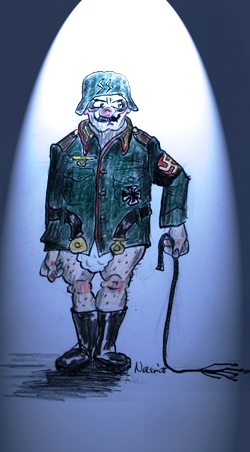
\includegraphics[height=60mm]{corps/chapitre6/img/personnage-avatar.jpg}
\end{floatingfigure}

Il relance néanmoins son holotar, lequel, la bite sous le bras, se met tout de go en chasse dans l’espoir de croiser sa belle valkyrie afin de la posséder comme une bête. Agacé, Timothée décide de modifier le programme. Fini le sado-maso, la sodomie, le hard. Et, tant qu’à y être, il n’y aura même pas de pénétration rituelle à la missionnaire. Rien ! Voilà plusieurs sessions qu’il ne prend plus de plaisir, ni moral, ni sexuel, à ce scénario. Ce soir-là, il n’y aura que poésie, romance, effets roses et passion platonique. Voilà ! Son avatar holographique sera un Roméo, un Abélard, un Tristan, en quête d’une Juliette, d’une Éloïse ou d’une Iseult. C’est dit, ce sera fait !

Dès lors, tout devient assez vite surréaliste. Roméo ressemble à un damoiseau italien du XVIe siècle, gerbe de fleurs à la main, portant haut-de-chausse vert, pourpoint bourgogne, dague décorative et chapeau sans panache. L’attricure a l’heur de déconcerter grandement l’avatar féminin habituel qui vient tout juste d’entrer en scène. C’est que son image est celle d’une sado-maîtresse bardée de fouets et de poings américains qui cache un petit bustier de cuir sous ses énormes tétons. L’apercevant, Roméo met quand même un genou à terre et lui présente ses fleurs. Mais, d’un rapide coup de fouet, Ilsa-la-louve les étête. Ensuite, d’un coup de botte, elle renverse Roméo et se met à le rouer de coups, cela jusqu’au moment où elle se retourne, le popotin bien en évidence, dans l’attente de sa rituelle sodomie. Visiblement, la personne derrière cet holotar n’a pas compris que Timothée entendait jouer sur un autre registre.

- Pause ! ordonne-t-il. Mode config ! IntentSync !

Tout s’est arrêté pour que les intentions des joueurs puissent être synchronisées par le truchement de Microsoft IntentSync 7.01. Mais il est possible qu’Ilsa ne veuille vraiment pas d’un Roméo ou que Roméo ne veuille vraiment pas redevenir Hans, le feldwebel SS botté et casqué. Les joueurs en ont le droit. Auquel cas, ils se quitteront pour se mettre à la recherche de partenaires leur convenant mieux.

- Reprise !

Le jeu redémarre, mais cette fois, Ilsa s’est transformée en Juliette, une Juliette forte du buste, du ventre et des hanches. De sa main calleuse, elle accepte les fleurs, sourit au beau Roméo et, d’un pas de caserne, va se placer sur son balcon, les yeux vers la pleine lune. En guise de poésie, le galant, les bras vers le ciel, entreprend alors de réciter le chapitre 3 d’un manuel d’instruction – celui du lecteur 3DVD - qui traîne sur le petite table près de Timothée. Si pour les avatars et leur programme informatique, le texte lu n’a aucun sens, quel qu’il soit, puisque ce n’est que du bruit, il en est tout autrement pour la personne derrière la grosse Juliette. Or celle-ci ne semble pas apprécier le scénario puisqu’elle le quitte, ce qui laisse Roméo tout seul et oblige son créateur à placer la session en mode pause.
Convaincu du bien-fondé de ses nouvelles valeurs, Timothée entend persister. Il se dépêche de dénicher et télécharger un fichier de poésie «précieuse» - du Du Bellay - et il l’ajoute aux «objets» pouvant enrichir ou compléter son avatar.

Contre toute attente, Juliette finit par réapparaître, une Juliette qui a été modifiée; on l’a fait maigrir. Elle commence à vraiment ressembler à une Juliette. Toute de blanc vêtue, elle est langoureusement appuyée sur la rambarde du balcon où elle semble attendre les mots d’amour qui la raviront au plus profond de son âme. Immédiatement, Roméo amorce son récital.

    Ces cheveux d’or sont les liens Madame,
    Dont fut premier ma liberté surprise,
    Amour la flamme autour du cœur éprise,
    Ces yeux le trait, qui me transperce l’âme.

    Forts sont les nœuds, âpre, et vive la flamme,
    Le coup, de main à tirer bien apprise,
    Et toutefois j’aime, j’adore, et prise
    Ce qui m’étreint, qui me brûle, et entame.

    Pour briser donc, pour éteindre, et guérir
    Ce dur lien, cette ardeur, cette plaie,
    Je ne quiers fer, liqueur, ni médecine,

    L’heur, et plaisir, que ce m’est de périr
    De telle main, ne permet que j’essaie
    Glaive tranchant, ni froideur, ni racine.

Juliette est émue. Très émue. La main sur le cœur, elle regarde son galant, puis, avec emphase romantique, lui jette une bague et, tout doucement, comme sur un nuage, s’éclipse du balcon. Roméo ramasse vivement le gage, verse une larme et, à son tour, disparaît de la cyberscène. Même Timothée ressent l’émotion.

Soudain, la console s’active et requiert son autorisation pour afficher une communication.

- Oui !

Sur le bas de cette scène désertée, on voit alors apparaître le texte 3D suivant :

- Qui es-tu ? J’aimerais te connaître.

Pris de panique, Timothée quitte le programme et ferme sa machine à quadruple tour.

- Si c’était la grosse Tremblay !

Il se dépêche jusqu’à la fenêtre de la porte d’entrée. En face, verre de bière à la main, Louis-Marc Richard est assis sur sa galerie en train d’admirer le soleil qui se couche à l’autre extrémité de la rue Crouet. Un instant, il quitte sa contemplation pour regarder son voisin, mais fait comme s’il ne l’avait pas vu.
Que sait-il, au juste, ce Judas ? À quel coup fourré doit-on s’attendre de lui ?

Et lui, Timothée, peut-être devrait-il garder les deux pilules ? Qu’est-ce que peut bien penser Robespierre de cette histoire ? Et, que penserait-il de cette autre histoire, celle impliquant la Bitch ? À moins que Juliette ne soit pas cette mocheté aussi dangereuse qu’un barracuda ! Arrivera-t-il, un jour, à avoir une blonde, une vraie fille en chair et en os ?

Malgré la brise presque saline qui chasse les maringouins, il décide de ne pas sortir prendre l’air – de toute façon, il ne le fait jamais – et d’aller se coucher. Comme d’habitude ! Une Mercedes électrique passe devant sa fenêtre sans faire plus de bruit que ces chauves-souris dont les hyperboles animent présentement le ciel de cette petite rue de Nazareth. Timothée pense alors à sa vieille Américaine sur le point de rendre l’âme. Où trouvera-t-il l’argent pour la remplacer ? Comment pourra-t-il s’occuper de tout s’il n’a pas de bagnole ? Faudrait-il en parler à Shimoune ? Demander de l’aide à Robespierre ? Car, qui sait, peut-être y a-t-il autre chose dans la vie, que cette guigne continuelle …
\chapitre{Le sort frappe, le mercredi 20 juillet 2033}{Accoté sur le devant de sa Subaru hybride, }{ Sébastien Larose, le dernier syndiqué de la fonction publique du Québec, observe avec délectation la petite foule qui manifeste devant l’entrée principale du CRG-BSL. La chaude brise matinale aidant, une trentaine de personnes, la plupart de jeunes sexagénaires encore productifs, psalmodient des slogans et brandissent des pancartes. Sur certaines, on a reproduit une image éloquente de Robert Gagnon, alias Dart Vader, empruntée au bulletin de nouvelles d’hier. Sur d’autres, on peut lire sur deux lignes «MONSANTO (biffé d’un X rouge)» et «MA SANTÉ!». Autour d’eux, une dizaine de journalistes ravis de cette aubaine médiatique captent tout ce qu’ils peuvent.}

- Non-non-non au manger mou ! scande-t-on par ici.

- Turco-otte, Turco-otte, Turco-otte, «mange d’la marde» répondit l’écho, chantonne-t-on par là.

Le bonhomme grimace un sourire, ce qui déforme légèrement son bouc plus sel que poivre. Pour la circonstance, il a choisi de revêtir son T-Shirt de la CSN, la grande centrale syndicale à laquelle il a adhéré l’an dernier. Comme il était le seul membre du Syndicat de la fonction publique du Québec, il n’avait eu aucune difficulté à organiser la manoeuvre. Surtout qu’il amenait en dote, un compte en banque appréciable.

\begin{floatingfigure}[l]{40mm}
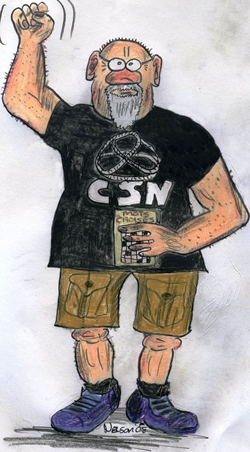
\includegraphics[height=60mm]{corps/chapitre7/img/personnage-sebastien.jpg}
\end{floatingfigure}

- On se croirait revenu à la belle époque. Salut mon homme, fait-il à Timothée qui vient de garer sa voiture à côté de la sienne.

Ainsi Dart Vader est devenu un symbole de lutte ! Pour Timothée, cela ne peut signifier que des ennuis, de très gros ennuis. Ce salaud de Dauphin, l’exécuteur des basses œuvres de Carl Michaud, le directeur général de l’établissement, va sûrement lui faire coiffer la responsabilité, donc la culpabilité, de cette atteinte à l’image de marque du Centre. Mais il se garde bien d’en glisser mot à Larose et file vers l’entrée latérale, celle qui donne directement sur le stationnement. Marie-Odile «la Bitch» Tremblay l’a précédé de quelques secondes devant l’ascenseur et la seconde et quart que durera la montée jusqu’au deuxième leur paraîtra, à tous deux, un siècle et demi. De toute évidence, évalue Timothée, l’agente de sécurité se retient pour ne pas parler d’holotar. Mais pour l’instant, Roméo Du Bellay dort à octets fermés; l’air de ce petit matin sent le concentré de mauvaises nouvelles.

À peine son dispositif personnel polyvalent (DPP) a-t-il avisé le système central de sa présence dans l’immeuble, qu’il se met à vibrer.

- Timothée Tardif !

- Ton chien est mort le Motté !

C’est Flipper Dauphin.

- De quossé ?

- Tu le vois le bordel qu’a créé ton bénéficiaire, ton bonhomme Gagnon ? Ben je vais te le faire récurer, mon salaud. J’m’en vais justement dans le bureau de Carl !

- J’ai rien à voir dans cette histoire, moi ! C’est toi et tes Papyblues qui avez mal fait votre travail…

Mais l’autre a coupé.

- Bof !

Qu’a fait de si terrible Robert «Bob» «Dart Vader» Gagnon, à part se plaindre du manger mou, de dire que ça lui donnait des coliques et de déclarer qu’on le punissait quand il se faisait prendre avec de la nourriture de contrebande ? Quoique à bien y penser…

Arrivé au cinquième, le CS-1 roule sa Saguewanish jusqu’au salon communautaire où une dizaine de vieillards se sont massés devant les fenêtres; la manifestation semble les intéresser.

Le père Jean ne peut se retenir :

- T’as vu, chef, y a encore du monde qui s’rappelle de nous autres !

Timothée laisse border. De toute façon, il n’y a pas plus de Dart Vader dans ce salon qu’il n’y a d’espoir pour une vie meilleure. Vivement, il repart vers le petit dortoir, une salle 2P, où il croit pouvoir le trouver. Pourtant, là non plus, pas d’homme à la canule.

- Il est parti en bas saluer son public, fait le vieux Martel.

- Où en bas, monsieur Martel ?

- En bas.

- Shit !

- Le prophète Abdias a dit : «Comme tu as fait il te sera fait : tes actes te retomberont sur la tête.»

- Ta gueule, Savoie, gronde Martel, tu nous écœures !

Mais Timothée est déjà en route vers le rez-de-chaussée. Sur place, il remarque son ami Shimoune Saint-Pierre, dit la grande folle du manger mou, en train d’écornifler. Partout, des agents de sécurité montent la garde et, près de l’accès à la cafétéria, un des sbires de Philippe Dauphin, soit Bluesly, soit Papynut, en tout cas, un des frères Côté, fait les cent pas, concentré sur sa boucle d’oreille. À ce qu’il semble, la plupart des pensionnaires ont choisi de se faire rares.

- Ils l’ont amené, annonce Saint-Pierre.

- Qui a amené qui, Shimoune ?

- Les Papyblues. Ils viennent de partir avec Dart Vader.

Saint-Pierre a imité le geste du bonhomme quand il appuie sur sa valve de phonation.

- Pour où ?

- Devine !

Et Shimoune de repartir vers son centre nutritionnel.

S’il n’était pas si «timoroso», Timothée foncerait sur-le-champ protester à la direction générale. Des gorilles ont escorté son pensionnaire vers l’inconfort du sous-sol où il sera puni pendant deux semaines ? Un mois ? Plus ? Cela, pour avoir dit publiquement ce qu’il pensait, pour avoir dit la vérité. Mais une esquive le sauve de sa couardise; son lobe d’oreille se met à frétiller.

- Timothé Tardif !

- Motté, c’est Laurent !

Encore des ennuis, soupire le CS-1.

- Alors ?

- Le père Lafrance vient de se lâcher, p’is ça pue la charogne. Y a plein de bénéficiaires qui chialent. Y a du vomi sur le plancher, sur la commode, sur les pattes du lit.

- Bon, je monte.

Arrivé au cinquième, il remarque, en croisant le salon communautaire, que la pièce a fait son plein de vieillards. Tout le monde est là et tout le monde a son idée sur la manif. Le pire, c’est qu’à l’exception de Jean Saint-Gelais, cet indécrottable délinquant, ils seront probablement tous ravis quand ils apprendront pour Dart Vader. Mais on n’y peut rien; c’est ainsi; le bonhomme l’a sans doute cherché.

Sauf que pour l’instant, il y a une urgence désagréable à gérer et ce ne sont ni Laurent, ni Mérovée, ni lui, qui nettoieront l’horrible dégât. Quant à faire venir une équipe du service d’entretien, c’est impensable. Il faudra patienter une bonne journée avant qu’elle ne se pointe. Il serait surtout important d’avoir une petite caisse garnie pour pouvoir bien arroser leur coordonnateur.

Cette annonce lui fait penser à la puanteur remarquée l’autre jour dans une des deux salles 2P-F, celles qui sont réservées aux femmes. Et puisque tout le monde semble être au salon, pourquoi ne pas en profiter, en chemin, pour aller redonner un coup de nez dans ce triste local, question d’en avoir le cœur net ? Bonne idée ! Mais en y entrant, le CS-1 tombe sur une scène romantique, mais pas encore torride, où, avec force soupirs, madame Thériault essaie de faire des choses discutables à madame Labbé dans le lit de cette dernière. Dieu du ciel !

- Que c’est que je vous ai dit avant-hier, madame Thériault ?

La rondelette créature se glisse en bas du lit et, en souriant à sa conquête, s’en va s’asseoir sur le sien.

- On faisait rien de mal, hein Jeanne ?

- B’en non, ment l’autre, une maigrelette aux allures d’alitée permanente.

Normalement, Timothée aurait baissé la tête et serait ressorti aux commandes de son bruyant Saguewanish. Mais pas cette fois. L’occasion est inespérée.

- Madame Thériault, si je veux, je n’ai qu’à descendre au 2e, aller à la Sécurité, leur demander un disque de la dernière heure ici dans cette salle 2P, amener ça au premier, chez les patrons, et, dix minutes plus tard, deux gros Papyblues qui haïssent les gouines, vont venir vous chercher, vous et madame Labbé, et ils vont vous descendre au sous-sol avec les autres foqués.

Il est venu près de dire «avec Dart Vader».

Les deux coquines déglutissent. C’est madame Thériault qui réagit, estimant probablement, en son for intérieur, qu’elle est la plus coupable des deux.

- Si tu veux ?

- Si je veux.

- C’est quoi le «si» ?

Timothée prend une grande respiration et il médite, une ou deux secondes, sur l’image de sa mère. Celle qu’elle avait avant sa réclusion dans un sous-sol de Nazareth. Celle qu’elle affichait quand elle lui enseignait si méchamment le trombone.

- C’est un plancher de vomi à nettoyer !

Grimaçante, madame Thériault est assez ratoureuse pour ne pas se mettre à hurler. Elle veut plus de détail.

- Le pére Lafrance, ici à côté dans la salle 3P-L, il a rendu tout ce qu’il avait dans le corps. Je vais devoir le transférer en palliatif. Pas drôle. Y a du vomi sur le plancher, sur la commode, sur les pattes du lit. C’est écœurant.

La bonne femme réfléchit un instant.

- J’peux-t-y avoir de l’aide ou faut que j’soye toute seule ?

- J’te vois v’nir, ma snoroune, s’insurge immédiatement l’autre coquine. C’est pas moi la turbo lesbo, c’est toi !

Timothée chasse une pensée fugace sur la mesquinerie de ses frères et sœurs humains.

- Celles qui torchent propre propre ne vont pas chez les foqués. Celles qui restent sur leur cul y descendent pour longtemps longtemps.

Une minute plus tard, le trio entre dans le dortoir des cas lourds en ce qui a trait à la perte d’autonomie. Une odeur épouvantable, soutenue de gémissantes protestations en provenance des lits, les accueille. Robespierre, en voisin de bureau, s’est arrêté près de la porte et tente de respirer le moins possible.

- Je peux te donner un coup de main ?

- Non, merci, t’es gentil. Mais j’ai ce qu’il faut.

Il pointe vers les deux délinquantes.

- Monsieur Lafrance, on s’en vient vous aider, annonce Timothée au grabataire souillé. C’est madame Thériault avec madame Labbé – vous les connaissez, non ? – qui vont vous ramasser ça. Quand elles ont appris votre malheur, elles se sont dépêchées.

Le bonhomme fixe le CS-1 de ses grands yeux noirs.

- J’veux pas m’en aller dans la salle palliative ! J’suis encore bon ! J’suis pas fini !

Timothée fait mine de rien et se retourne vers les deux femmes.

- Les moppes, les guenilles, le savon sont dans le placard 5-PP67, juste à côté dans le couloir. Je vous l’ouvre.

Il appuie alors sur son sa boucle d’oreille et déclame :

- Ouverture ! CS-1 Timothée Tardif ! 5-PP67 ! Oui !

Ce qu.entendant, les commères vont quérir leur matériel. Rassuré, le fonctionnaire manœuvre son Saguewanish vers la porte en contournant l’immonde flaque du père Lafrance. Mais celui-ci veille au grain et il tend la main.

- Attends une minute, mon ‘tit Motté, j’ai un cadeau pour toé !

- Un cadeau ?

- Pour rester ici, pour pas aller chez les morts. J’ai ramassé 642 piastres.

Mais il n’a pas de bout de papier avec un code inscrit par Solange Gadoury. Le CS-1 commence par vouloir décliner, par vouloir lui crier que c’est trop, que la situation est horrible, par vouloir lui jurer qu’il refuse de lui voler ses dernières économies, qu’il en aura besoin quand il sera en SP en train d’attendre la prochaine cérémonie de groupe. Mais, encore une fois, l’image de sa mère vient se substituer. Quelle tempête elle fera si elle apprend qu’il a refusé 642 \$ ! Ainsi, Timothée accepte en fuyant le regard du moribond. Pour la Maririou, pour Romain, il prendra cette somme, pour peu que la mère Gadoury lui en donne le code.

Auquel cas, par la volonté d’un fonctionnaire qu’il vient de graisser, Jean Lafrance ne sera pas conduit dans l’antichambre de la mort du 5e Nord. Du moins pas pour l’instant.

Une voix se fait entendre du couloir, celle du bonhomme Saint-Gelais.

- Vous vous êtes faites pogner, les gouines ?

- Étouffe-toi donc, vieux maudit, lui rétorque la mère Thériault.

Tout au fond de son sombre local, le vieux Asselin est assis à la noirceur, dans l’unique fauteuil de la pièce.

- Pas besoin d’avoir des yeux pour savoir qui vient me voir sur sa bécane. Y a seulement la tienne, chef, qui fait tant de bordel.

- Bonjour Monsieur Asselin. Comment ça va aujourd’hui ?

- Juste au son, ton moteur devrait sauter d’ici dix à quinze kilomètres.

Timothée fouille dans le porte-documents accroché à son Saguewanish.

- Branchez-vous ce lecteur à l’oreille. J’y ai mis l’œuvre complète de Tchekhov.

Les lèvres du vieillard tremblent et ses longs doigts se referment sur le gadget chinois.

- Je pèse où pour que ça parte ?

Timothée lui place la main au bon endroit.

- Essayez de dormir quand même.

L’entorse au règlement risque de lui faire chauffer le matricule si les cafards télécommandés du 2e attirent l’attention d’un agent de sécurité (agente de sécurité ?) mal intentionné. Mais il s’en fiche. Il éprouve même une grande satisfaction de l’avoir fait.

Encore une fois, l’oreille lui chatouille. Décidément !

- Timothée Tardif !

C’est la voix de son père.

- Viens-t-en vite. C’est ta mère ! Elle n’arrête pas de saigner.

- Maman ?

- Ça a commencé tantôt.

Du sang, sa mère saigne. Le cœur de Timothée s’est accéléré.

- Elle saigne, comme une hémorragie ?

- Oui. Ça vient d’en dedans. Ça lui sort par le milieu. Je sais plus quoi faire !

Sans aviser quiconque, en évitant de regarder Bea Bellow qui, livres en main, a tenté d’attirer son attention, le fonctionnaire file vers le stationnement et roule, le plus vite qu’il le peut, jusqu’à chez lui.

Plein d’appréhensions, Timothée veut descendre l’escalier. Mais Gazou, le chien-rat, lui bloque l’accès. La sale bête semble enragée au point de vouloir le mordre. Sans hésiter, il l’attrape par la tête et, comme s’il s’agissait d’une peluche que l’on jette aux rebuts, la propulse littéralement à la rue.

- Kaï kaï kaï !

Vive les colliers GPS !

En bas, il trouve son père assis sur le bord du lit où geint une Maririou en état total de panique. Il lui a placé des serviettes, mais, il ne fournit pas. On dirait que la vieillarde est en train de vidanger son méchant. En plus de ne rien comprendre de ce qu’il lui arrive, elle voit bien le dégât causé par ses saignements abondants, ce qui a l’heur de l’angoisser davantage.

- Mon Dieu Cheigneur, qu’est-che qui m’arrive ? Que ch’est que je vas faire ?

Sidéré, Timothée se tait. Il regarde, il essaie de comprendre. Elle saigne ! Elle coule ! Et du vagin ! Sa mère ! Comment pourrait-il arriver à la toucher, à toucher au vagin de sa terrible mère, au terrible vagin de sa mère ? Il a beau connaître les premiers soins, il est impuissant.

- Va vite me chercher d’autres serviettes. Dépêche !

Tandis que le fils accourt jusqu’au placard lingerie, comme s’il voulait fuir le long geignement sans accalmie de sa mère, Romain, lui, ne réfléchit plus. Il éponge le pire. Il maintient une serviette sur la source morbide. Il tente de se faire rassurant.

- C’est moins pire que tantôt, ment-il à sa compagne dont la pâleur commence à être inquiétante. On dirait que ça ce calme.

- J’vas mourir, Romain.

- Tais-toi donc. Ça va s’arrêter. Crois-moi !

Et là, phénomène excessivement rare, la Maririou se met à pleurer d’un sanglotement effrayé, charnel, profond, une longue plainte qu’on dirait associée à la mort, une insoutenable lamentation où on peut décoder quelques « j’vas mourir ». Gauchement, Romain essaie de la réconforter, mais, comme peut le constater le fils, il n’y arrive pas du tout. La panique est même en train de le gagner. On n’a plus le choix; il faut d’urgence aller chercher de l’aide. De l’aide discrète, si possible !

\begin{floatingfigure}[l]{40mm}
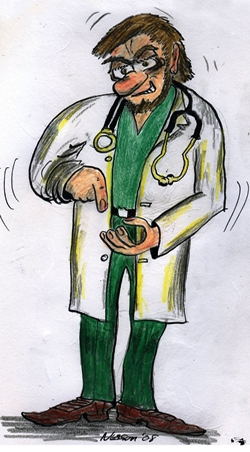
\includegraphics[height=60mm]{corps/chapitre7/img/personnage-etienne.jpg}
\end{floatingfigure}

- Y a Étienne Gagnon, dit-il d’un ton deux coches trop élevées. C’est un des médecins du Centre, un gars qui trempe dans toutes sortes de combines.

- Y est-y capable de soigner ta mère ?

- Il connaît son affaire, mais ça va nous coûter un bras et on n’a même pas 2 000 \$ dans le compte !

- On n’a pas le temps de calculer, va vite le chercher !

Timothée file et, sans un regard pour Gazou qui voudrait bien revenir vers sa maîtresse, fait démarrer son antiquité sur les chapeaux de roues. D’un tic de l’index sur sa boucle d’oreille, il demande à la réception du Centre si le docteur Gagnon est sur place où s’il est à sa clinique privée du quartier Saint-Germain, un secteur assez huppé de Rimouski. La deuxième possibilité serait vraiment géniale, se dit-il.

La chance lui sourit. Non seulement le médecin y est, mais il accepte de le recevoir entre deux rendez-vous.

Devant la gravité de la situation, le toubib met fin abruptement aux négociations.

- Ça sera mon prix ! C’est à prendre ou à laisser. On n’a pas le temps de négocier; ça presse !

Comme son interlocuteur donne un signe d’acquiescement, il demande à sa réceptionniste d’informer tout le monde qu’il a dû partir pour une urgence et d’essayer de tout décaler de deux heures.

- C’est beau, je te suis !

Une heure plus tard, Marie a cessé de saigner et, la bouche édentée grande ouverte, elle dort avec bruyante application. Et pour cause; Gagnon, en émule de vétérinaire, lui a administré un sérieux cocktail pharmaceutique. Il a toutefois fallu que Romain mette Gazou sur la petite galerie face au fleuve, la mauvaise bête s’étant réintroduite dans la maison à l’arrivée des secours, une arrivée hautement remarquée par Louis-Marc Richard, d’ailleurs.

- Elle a quoi ? demande Romain.

- Un beau cas de métrorragie ou, si vous préférez, d’hémorragie postménopausique. C’est clair qu’il y a un problème à l’endomètre. À son âge, ce sont peut-être des polypes endométriaux, des polypes qui sont là de façon latente depuis des années. Sinon, il peut s’agir d’une tumeur. Faut aller voir.

- Une tumeur ? Un cancer ?

- Les tumeurs ne sont pas toujours malignes.

- Faut aller voir comment ?

- Faudrait lui passer une échographie. J’ai ce qu’il faut, un système portatif Bluetooth Azure. Si ce sont des polypes, on verra pas grand-chose. Mais si c’est une tumeur, on verra une masse. Malheureusement, on ne pourra pas savoir si elle est cancéreuse. Pour le savoir, va falloir une analyse sanguine avec une recherche spécifique de marqueurs susceptibles de confirmer ou d’infirmer la présence de cancer. Sauf que ça va coûter des bidous; mon technicien ne vit pas avec l’air du temps !

- Seigneur !

- S’il y a tumeur, cancéreuse ou non, il faut l’enlever. Et là aussi, j’ai ce qu’il faut. Je peux pratiquer ici même une hystéroscopie qui pourra régler le problème. Évidemment, il lui faudra du repos et une médication appropriée, peut-être pas des progestatifs à son âge, mais quelque chose pour éviter l’infection, favoriser la cicatrisation et réduire la douleur.

- Ça a pas de maudit bon sens !

- Il va falloir que je revienne avec mon matériel médical le plus tôt possible, possiblement demain en matinée. En attendant, vous lui faites prendre ces pilules-là et celles-là, trois fois par jour, juste avant de manger.

- Oui mais docteur, balbutie Timothée, on n’est pas capable de payer tout ça !

Gagnon caresse son collier de barbe.

- Je sais. Tu ne roules pas sur l’or et, en bon fils, tu te saignes pour héberger tes parents, deux Boomers illégaux. Si je te demande de l’argent, tu vas péter au frette ! Donc je ne t’en demanderai pas.

Le cœur du «bon fils» veut lui sortir de la cage thoracique.

- Mais …

- … je vais te demander un petit service.

Timothée ravale cette salive fétide qui lui gâche l’haleine.

- Un service ?

- Oui. Il me faut certains produits, des produits pharmaceutiques, parmi ceux qu’ils utilisent au centre nutritionnel pour «assaisonner» les plats de Nutrisuz. Peux-tu m’aider ?

- Des produits pour ma mère ?

- Non. Ça rien à voir. C’est pour ma business. C’est donnant donnant. Je soigne ta mère, tu me procures des produits dont j’ai besoin pour d’autres patients.

Horriblement angoissé, le quadragénaire enlève ses verres et les essuie avec le pan de sa chemise. Dehors, Gazou a cessé de japper et a commencé à hurler.

- Il va nous attirer les voisins ! Déjà que tantôt, Louis-Marc Richard nous a vu arriver, le docteur et moi !

Romain lui ouvre la porte et, du pied, l’oblige à demeurer dans la chambre de sa maîtresse. Sauf que Gazou est déchaîné.

- Tais-toi, asti de chien fifi ! J’vais te fesser à coups de soulier !

Comme s’il avait compris, le chien jaune s’en va renifler près du lit de la vieillarde et, prouesse étonnante compte tenu de son embonpoint et de la longueur de ses pattes, saute sur l’édredon recouvrant la malade.

- Je veux bien vous aider, docteur, mais je n’ai pas accès aux produits pharmaceutiques du Centre, moi. Le seul qui puisse pigrasser là-dedans c’est Amédée Chicot. À part lui, je vois pas qui peut vous aider. Mais ça, vous devez bien le savoir ?

Tandis qu’il referme soigneusement sa petite mallette de toubib comme il y en avait dans les anciens films, il lève les yeux en direction de Timothée.

- Je vais te dire comment je vois ça. Tes parents, ta mère surtout, ont un urgent besoin de soins professionnels et mon serment d’Hippocrate m’oblige à m’assurer qu’ils en aient. Or voilà que je peux leur en fournir, mais c’est ainsi que ça fonctionne, il y a des frais, des frais que tu dois assumer. Si tu n’es pas capable, mon devoir est de m’assurer que tes vieux parents reçoivent quand même des soins. Et dans le domaine du gratuit, je ne vois pas d’autre solution que celle du CRG.

- Oui, mais mes parents sont illégaux …

- C’est pas mon problème. Leur santé, que dis-je, leur vie passe avant tout.

- Je sais, mais …

- Écoute, je ne te demande pas le Pérou. Y vraiment rien d’extraordinaire là-dedans. Depuis que c’est Michaud qui est DG au Centre, tout le monde se sert; le vol est devenu pandémique. Prends le temps d’y penser, d’imaginer une solution et fais-moi signe quand tu auras trouvé … disons d’ici une semaine ?

Sur cette tirade, le bon docteur gagne la sortie.

Complètement défait, accablé, découragé, Timothée arrive quand même à voir le salopard disparaître dans l’escalier, accompagné du chien-rat hurlant de toute sa haine. Une lueur assassine aux yeux, le toubib tente, d’un rapide coup de pied, de le faire retraiter, mais Gazou esquive le danger et poursuit son insupportable manège. Encore une fois, Romain doit s’en mêler.

- Gazou, ciboire de bâtard de chien débile, ici, au pied !

Subodorant les conséquences d’avoir fait lever le bonhomme, l’horrible roquet retourne se réfugier en grondant auprès de sa maîtresse.

- Serment d’Hippocrate, serment d’Hippocrate ! Sacrament d’hypocrite de maudit hypocrite de sacrament !, sanglote nerveusement Timothée sans regarder son père.

Comment il va faire pour dénicher les produits que convoite Étienne Gagnon ? Tout est tellement surveillé dans l’établissement ! Quand bien même qu’il en parlerait à son ami Shimoune, ça ne donnerait pas grand-chose. Tout au plus connaîtrait-il les heures où il est possible de passer au centre nutritionnel sans qu’il n’y ait de préposés. Mais encore là, sans code pour déverrouiller la remise pharmaceutique, comment pourrait-il aller plus loin ? Arriver avec une hache de sapeur camouflée dans sa chemise ? Avec une pince monseigneur ? Soyons réalistes! Et la pire difficulté n’est même pas à ce niveau. Elle est au 2e, chez les gens de la Sécurité qui, avec leur électronique de pointe, voient tout et entendent tout à la grandeur du bâtiment. Pire, des détecteurs savent déceler les articles qu’apportent, cachés ou non, les employés qui entrent dans l’établissement ou qui le quittent.

Soudain, un flash lui permet d’extirper d’un recoin perdu de sa mémoire le nom de cet ouvrage d’Orwell qui lui avait traversé l’esprit l’autre jour : 1984 !

L’inquiétude lui rongeant le système, Timothée regarde sa montre; il n’est pas encore 13 heures. Il doit absolument retourner au Centre pour régler quelques trucs; il ne faut quand même pas attirer l’attention. Vérification faite dans sa boucle d’oreille, il sait qu’aucun message de Carl Michaud ou de Flipper Dauphin ne lui est parvenu. Bonne nouvelle ? Pas certain ! Demain c’est la réunion du Comité de déontologie dont il fait partie et où siègent ces deux hauts gradés. Il est probable qu’ils en profiteront alors pour lui faire sentir leur courroux.

- Je reviens dans une heure, fait-il à son père qui, malgré l’hostilité de Gazou, est retourné s’asseoir sur le bord du lit de sa vieille compagne.

Comment ne pas penser à cette énorme tuile qui vient de lui fracasser son misérable ordinaire ? Comme faire semblant qu’il n’y a aucun problème à part sa trottinette qui est en train d’agoniser bruyamment ? Dans sa salle palliative où il se rend tout d’abord pour bricoler de la paperasse en vue de la Cérémonie de groupe du 3 août prochain, une vieille dame, l’occupante du lit no 5, lui fait un signe discret. Quand il se penche sur sa couchette, elle lui dit qu’elle ne veut absolument pas «assister» à la «prochaine célébration» et qu’elle a un petit accommodement à lui proposer.

Outre l’aspect extraordinaire du fait qu’il s’agisse de la deuxième tentative de pot-de-vin de la journée, ce qui rend ce cas vraiment touchant, c’est que la mère Gadoury n’a pu lui dénicher que 200 \$. À ce tarif, on s’en doute bien, personne du CRG-BSL n’accepterait de trafiquer un dossier de bénéficiaire. Mais Timothée, lui, il y consent. Le regard de la mourante est tel, qu’elle ne lui aurait offert que dix sous et il aurait dit oui. Le 3 août, c’est dans quinze jours et, pense-t-il, la pauvre dame, dans l’état où elle est, ne vivra sûrement pas jusque-là. Le calcul est simple : si ce n’est pas lui qui empoche les 200 \$, ce sera le Centre, c’est-à-dire le gouvernement. Cet État on ne peut plus vorace. Aussi bien que l’argent serve à ceux qui en ont vraiment besoin. De toute façon, eux, ces vieux qui casquent à coups de petits 200 \$, ils se paient de l’espoir sur leur grabat de mourant. Et ça, c’est bien. Oui mais le mythique Timothée de Milet n’aurait sûrement pas, lui, accepté de fric, lui, et aurait vidé l’établissement de tous ses profiteurs à grands coups de lyre à onze cordes. Mais, bof !

Dans son bureau, il aimerait pouvoir vérifier et modifier la fiche de cette mourante, ne serait-ce que pour s’occuper les méninges, pour donner aux autres l’impression que tout est comme d’habitude, que sa mère ne vient pas de chambouler inexorablement le scénario de leurs trois vies. Mais, encore une fois, rien ne fonctionne du côté informatique centrale. Ne reste plus qu’à tout fermer et rentrer à la maison ! Comme s’il pouvait y avoir présentement un ailleurs !

Rue Crouet, il retrouve son père assis devant une télé sans audio, perdu dans ses pensées. Le vieillard le salue vaguement de la main. Gazou n’a pas jappé. Couché sur le bout du lit où ronfle la Maririou, il s’est contenté de gronder.

- Tire-toi une bûche.

Mais Timothée sait que la conversation sera difficile. Romain est amer. Ce qui devait arriver s’est produit. Sa Marie est tombée gravement malade. Plus rien ne va et demain sera encore plus épouvantable qu’aujourd’hui. Il ne peut en être autrement. Si ce n’est ce «crosseur de médecin» qui va les dénoncer, ce sera le voisin d’en face, cet «enfant de chienne» de Richard qui le fera ! Est-ce la fin du parcours ? Est-ce un aller simple vers les geôles du CRG ? De toute façon, avec cette maladie, il doit être devenu trop tard, maintenant, pour vraiment considérer la fuite vers Anticosti.

- Oui, mais j’ai pas eu le choix, fallait que je me grouille ! Et mis à part le docteur Gagnon, je ne voyais personne d’autre !

- Je sais. Tu as fait de ton mieux. C’est pas après toi que j’en ai, mais après le sort !

Timothée ravale un sanglot.

- Ta mère avec son caractère de chien, avec ses exigences jamais satisfaites, elle t’a toujours beaucoup aimé.

Et le bonhomme que l’on dirait claquemuré dans ses souvenirs se lance dans l’exposé sans fioritures, d’un pan de vie que Timothée aurait tellement souhaité pouvoir oublier. Un pan qui aura duré presque dix ans et dont les protagonistes étaient sa mère et lui. Résigné, il réentend l’histoire de cette matrone sans pitié qui, soir après soir, lui faisait refaire ses devoirs, reprendre ses études, récapituler ses leçons. Encore une fois, son père lui raconte la persévérance de cette femme autoritaire qui, année après année, tenait tête aux enseignants, aux spécialistes, aux directeurs d’école qui voulaient de concert recaler son cancre de fils, l’affecter aux classes spéciales ou le changer d’institution. Il laisse Romain lui remémorer le calvaire de cette Maririou avare de sourire et dépourvue d’affection, qui l’avait amené à réussir, bien malgré lui, son primaire, son secondaire et, en partie, son collégial. Dieu qu’elle lui en avait fait baver !

- Mais, elle a jamais pu dire «je t’aime» à personne. Ni à moi, ni à toi !

Dans sa chambrette voisine, la Maririou s’est mise à balbutier d’incompréhensibles arguties.

Le fils enlève ses verres et, des paumes, se frotte les yeux brûlés d’émotion. Que peut-il faire ? Est-ce la fin de ses parents ? Deviendront-ils les prochaines proies des flics du BAG ? Et lui ? Qu’arrivera-t-il de sa carrière une fois que toute l’histoire aura été révélée ? C’est jeune, 43 ans, pour vivre dans la dèche, pour faire de menus travaux afin de pouvoir manger et être soigné, pour aller changer des couches de vieux sous les quolibets de tout le monde, y compris des incontinents eux-mêmes. Existe-t-il une solution ? Est-ce possible de la découvrir d’ici une semaine ? C’est court une semaine ! Le temps est-il venu d’utiliser les pilules de Robespierre ? Faudrait-il commencer à en parler à Romain ?

La peur et l’angoisse le font plutôt filer. D’une traite, il se rend jusqu’au cimetière tout près de sa maison. Lentement, il s’appuie sur la clôture, comme pour mieux goûter l’air parfumé de cette superbe journée de juillet, un air venu tes terres plus au sud, un air très doux où les effluves d’avoine fraîche laissent passer celles, plus sucrées, du trèfle rouge. Derrière lui, plus loin, à sa droite et à sa gauche, des éclats de joie, de plaisir sportif, de jeux d’adultes lui parviennent. Nazareth semble d’humeur joyeuse. Il fait beau, les gens sont heureux. Même les morts du cimetière doivent l’être. Le seul qui ne l’est pas c’est lui, ce bon fils d’une mère très malade dont la vie, jusque-là pas si extraordinaire, est en train de basculer, par son sang, vers le pire des cauchemars.

Méchante journée !
\chapitre{Déontologie à gogo, le jeudi 21 juillet 2033 }{Ce qui, en temps normal, }{impressionne le plus Timothée et Shimoune quand ils viennent se caler, côte à côte, dans leur fauteuil de la salle du Conseil d’administration pour leur réunion mensuelle du Comité de déontologie de l’établissement (CDE), ce n’est pas la charretée de propos aussi doctes que biscornus, ni les yeux haineux de Philippe Flipper Dauphin, ni le regard impénétrable de Carl Michaud. Non, c’est le décor ambiant. C’est comme si les trois quarts de la masse budgétaire consentie à la décoration du CRG-BSL lors de sa construction avaient été affectés à la salle du CA. On se croirait à Balmoral, ce palais de la reine Victoria. Tout n’est que boiseries, caissons, frises, lustres, cuirs et tapis. De quoi séduire et rassurer n’importe quel banquier, n’importe quel politicien, n’importe quel philanthrope. }

S’il avait son mot à dire, le fils Tardif, il y a belle lurette qu’il aurait transformé la somptueuse pièce en bibliothèque classique, sombre, feutrée, sentant le bouquin poussiéreux, où, de temps à autre, entre deux décès survenus dans son parc à vieux, il irait se recueillir dans une méditation extatique, question d’oublier le caractère insoutenable de sa vie de Motté, de CS-1 du 5e Nord, d’enfant unique d’une Maririou saignante, blafarde, terrible. 

Paradoxalement, les trois carafes d’eau disposées sur la longue table semblent avoir été ramassées dans une vente-débarras et les verres sont en petit plastique cassant. Sur le mur du fond, immédiatement derrière le fauteuil du président d’assemblée, un cadre aux moulures XIXe représente le ministre Turcotte dans toute sa magnificence. Pourquoi pas une statue équestre devant l’entrée principale !

On devine que ce matin, Timothée a la tête bien loin des soucis bibliothéconomiques ou des aménagements de monuments. Non pas qu’il rumine, comme il le devrait, l’affaire Dart Vader Gagnon dont en haut lieu, on veut le coiffer. Il est plutôt aux premières lignes de ce désastre appréhendé dont le processus a été enclenché hier avant-midi par sa mère. Il n’a d’images que les draps souillés de sang, la pâleur de la possiblement cancéreuse Maririou et l’abominable commande du Dr Gagnon.

- Une chance que tous les Gagnon ne se ressemblent pas, pense-t-il un instant.

Pourtant, les deux risquent de lui faire perdre son boulot : l’un parce qu’il le force à voler des produits pharmaceutiques, l’autre parce qu’il a critiqué l’établissement dans les médias, ce qui est encore pire.

C’est à peine s’il suit le débat surréaliste portant sur la nature des soins qu’il est «administrativement possible» d’apporter aux pensionnaires en perte d’autonomie, ceux que l’on garde dans les salles 3P. Voilà des gens, pour la plupart, atteints de démence, de sénilité, de maladies incurables, des gens dont «les coûts d’entretien sont imprévisibles». Dans un contexte où les deniers sont rares, où la société doit financer ses universités, favoriser les études de pointe, aider la jeunesse talentueuse à acquérir les formations les plus pointues, a-t-on moralement le droit de dépenser des centaines de milliers de dollars sur une opération dont le bénéficiaire, un vieillard lourdement affaibli, un baby-boomer qui, sa vie durant, aura commis tous les excès, passera, de toute façon, en salle palliative (SP) quelques semaines plus tard ?

Sur un bout de papier, l’irrévérencieux Shimoune a dessiné un doigt d’honneur et le lui montre discrètement.

Quand un pensionnaire commence à souffrir de démence, pourquoi devrait-on lui fournir d’onéreux services ophtalmologiques, sachant que, de toute façon, elle ne lira plus de livres ou ne consultera plus de systèmes informatisés ? N’est-ce pas là du gaspillage ? Ou encore, pourquoi devrait-on sauver la prostate d’un octogénaire alité, le duodénum d’une vieillarde incontinente, l’ouïe d’une insomniaque médicamentée, la hanche d’une personne dépressive passant le plus clair de son temps couchée ?

Et de chuchoter son comparse :

- La queue d’un bande-mou ?

\begin{floatingfigure}[l]{40mm}
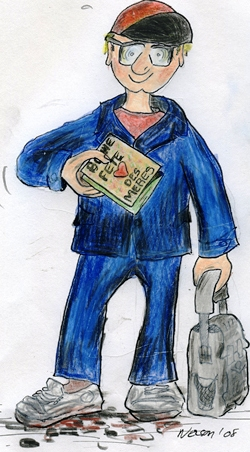
\includegraphics[height=60mm]{corps/chapitre8/img/personnage-timothee-jeune.jpg}
\end{floatingfigure}

Et la vie d’une vieille femme qui a des polypes endométriaux ou une tumeur peut-être cancéreuse, une vieille femme qui n’a pas encore été capable de dire «je t’aime» à quiconque, une vieille femme malgré tout attachante, doit-on la prolonger le plus longtemps possible afin qu’un jour, elle finisse par connaître la chaleur d’une relation affectueuse avec un fils lourdement perturbé ? Combien d’années de lucidité reste-t-il à cette femme brillante ? Dix ? Plus ? Moins ? Il y aurait tellement de choses à lui déclarer, à préciser, à expliquer, à se souvenir.

Se rappelle-t-elle de cette fête des Mères - Timothée devait avoir douze ou treize ans - où il était arrivé de l’école avec un important bricolage en papier gouaché, découpé, collé, broché, une carte de souhaits à rabats, sur laquelle il s’était appliqué toute la semaine ? Mais la pluie ayant créé des flaques de boue ici et là, le gamin s’était crotté les chaussures à la sortie de l’autobus scolaire et, en entrant avec son gage d’amour filial brandi à bout de bras, il avait souillé le plancher. Ce que voyant, la Maririou s’était mise à crier. Elle lui avait arraché la carte des mains, lui avait fait retirer ses galoches et l’avait enfermé dans sa chambre. Il n’avait jamais revu son œuvre et n’en avait plus jamais fait d’autres. Dans ses souvenirs, c’était la dernière fois qu’il avait tant pleuré. Perception d’enfant gravée à tout jamais au détriment des faits réels ? Allez savoir !

À son tour, Jacques Leblanc, un agent de recherche du ministère, économiste de formation se targuant de certaines connaissances actuarielles, se lève, et, de son dispositif personnel polyvalent (DPP), le modèle évolué et nécessairement corpo, projette des tableaux, des courbes, des boîtes couleur, où il est clairement démontré qu’à la grandeur du Québec, la durée moyenne de séjour dans les salles communautaires pour personnes en perte d’autonomie (SC3PA), c’est-à-dire les 3P, cas mineurs (3P-M) et lourds (3P-L) confondus, est de huit mois, treize jours et dix heures. Si c’est «nettement meilleur» que la moyenne canadienne qui est de neuf mois, vingt-deux jours et quatre heures, ce constat amène néanmoins une réflexion sur la «pertinence d’investir médicalement dans le contexte d’un tel état de fluidité».

- Les courbes de roulement que nous avons établies témoignent d’une dynamique très active et d’une constance remarquable; certaines provinces nous envient. Pour tout dire, nous pensons que ce serait jeter de l’argent à l’eau que d’augmenter l’enveloppe sanito curative, conclut-il.

- Sanito curative ? questionne le président d’assemblée.

- Euh, clinique, poursuit le fonctionnaire Leblanc.

Autrement dit, pourquoi rénover un appartement quand on sait que l’immeuble sera détruit dans huit mois ? Pourquoi voler des produits pharmaceutiques au profit du docteur Gagnon afin que Marie Rioux guérisse, une illégale qui a déjà un pied dans la tombe ?

- Ce n’est pas là dépenser les fonds publics de façon éclairée.

Le brillant exposé est terminé et quelques participants se dépêchent de féliciter l’orateur. Suit alors un silence qui frigorifie la pièce pourtant lourdement climatisée. Timothée se demande s’il ne serait pas possible, de nuit, d’arriver à faire monter un long tuyau galvanisé jusqu’au 5e Nord où l’on pomperait un peu de cet air rafraîchissant dans certaines salles, par exemple dans celle où sévit le tandem Thériault-Labbé, dans celle où repose Pierre Asselin ou même dans ce misérable coqueron de bureau qu’on lui a assigné.

- Mais ce sont des êtres humains, réfléchit un psychologue de pratique privée à la manière d’un camion qui frappe de plein fouet un pilier de béton.

Tiré de ses ruminations, Timothée est témoin d’une envolée implorant les considérations humanitaires et qui se termine sur une note plus politique.

- Cette génération a sûrement ses torts comportementaux, mais est-ce de sa faute ? Mérite-t-elle un tel châtiment ? Ne sont-ce pas les Boomers qui ont débarrassé le Québec de sa mythologie religieuse et qui en ont fait cette puissance économique respectée partout au Canada ?

Au lieu d’assister à une salve d’applaudissements, on entend plutôt la voix courroucée d’un «rouleur de r».

- Quelle mythologie rrreligieuse, s’insurge un médecin membre influent de l’église néo-évangéliste du Bas-Saint-Laurent. Si rrremplacer le Chrrrist et l’Évangile par la drrrogue, l’alcool et les maladies honteuses est pourrr vous un accomplissement, cette générrration mérrrite d’être enferrrmée au pain et à l’eau dans des salles en désorrrdre, leurrr élément de prrrédilection …

- Mange don’ d’la marde, interrompt Jipé Gendron, alias Tit-mononk, un pensionnaire en 2P qui représente les bénéficiaires sur ce comité.

Tandis que Philippe Dauphin prend des notes, ses yeux noirs sur cet émule de Dart Vader, l’avocat Rémi Anglehart, président d’assemblée et conseiller juridique de l’établissement, se dépêche d’intervenir.

- Messieurs, messieurs ! On se calme. On ne quitte pas cette harmonieuse civilité qui nous caractérise.

- J’ai fait mon point, conclut néanmoins le médecin rrrouleur, ce qui oblige Tit-mononk Gendron à avoir le dernier mot :

- Crétin !

Puis devisant l’économiste :

- As-tu fait des calculs pour savoir combien de vieux de plus, tu pourrais rentrer dans les centres en réduisant d’un pied la largeur des lits ? Ou en les mettant à deux étages, les incontinents en bas, les propres en haut ? Et pour sauver, tu pourrais couper de moitié le nombre des matelas : on aurait un jour «avec matelas» et un jour «sans». Tant qu’à y être, pourquoi tu leur dis pas, à tes boss, de rendre obligatoire partout le projet du Dr Bellavance. Au moins là, on pourrait devenir rentables, nous autres les vieux ! Crétin !

- Monsieur Gendron, s’il vous plaît !

- J’ai pas fini de parler, Anglehart, ‘sti ! T’auras rien qu’à m’envoyer rejoindre Dart Vader dans vos geôles du sous-sol, chez les Papyblues !

Les traits de Carl Michaud se contractent au point de ressembler à ceux de Flipper.

- Les générations X et Y reprochent aux baby-boomers de ne pas avoir fait assez d’enfants, poursuit le bonhomme. Mais quand je vous vois, toute votre gang de crabes en train de calculer combien de grammes de manger mou vous pouvez nous chipoter pour mieux équilibrer vos sacraments de budgets, je pense que les baby-boomers en ont fait beaucoup trop d’enfants. Ils auraient dû tous faire comme moi, se faire vasectomiser à 28 ans !
Me Anglegart commence à s’échauffer.

- Monsieur Gendron, vous vous emportez et ça n’avance en rien le débat.

- Point d’ordre, monsieur le président, le représentant des bénéficiaires nous fait perdre inutilement du temps ! Après ça on se demande pourquoi des gens de mon âge traitent de «vieux dégénérés» certains spécimens – il pointe vers Tit-mononk - de cette génération !

C’est un jeune homme à la mine fort grave, le délégué du Conseil de développement économique régional, qui a parlé.

- M’a t’en faire des «vieux dégénérés» p’tit fasciste néolibéral ! rétorque aussitôt le vieillard.

L’officiant ès procédure s’étire les bras. Il est sur le point de perdre le contrôle.

Noblesse oblige, c’est Carl Michaud, le DG, qui le tire immédiatement d’affaire. Il a levé un doigt.

- La parole est à monsieur Michaud, notre bon directeur général, prononce nerveusement le président par-dessus le tohu-bohu.

Une main en l’air, il se retourne vers Claude Sey, un jeune rédacteur au service de la direction des communications qui fait office de secrétaire d’assemblée.

- Monsieur le secrétaire, veuillez ne pas considérer dans le compte-rendu, les échanges impliquant M. Gendron.

- J’efface tout ?

- Tout. Je m’en porte responsable, précise l’avocat en faisant un signe de tête au grand patron.

Tous se taisent. Carl Michaud a pris la parole.

- J’aimerais demander au représentant des chefs de section, ces professionnels qui sont en contact direct et quotidien avec nos bénéficiaires dans les salles communautaires pour personnes en perte d’autonomie, les 3P, ce qu’il pense de la question, à savoir, la nature des soins qu’il est administrativement possible d’apporter à ces pensionnaires mal en point. Qu’en dites-vous, monsieur Tardif ?

Horreur consommée ! Voilà la punition que le patron a décidé de lui infliger : prendre la parole devant une longue tablée de bonzes, de médecins, d’avocats, d’administrateurs, d’ingénieurs, d’économistes ! Lui qui n’a qu’un certificat d’études collégiales. Lui qui n’est qu’un Motté rase-mur qui ne voit que les godasses des autres, qui ne perçoit que leur choc, plus ou moins amorti selon les personnalités, sur le plancher ! Lui cet être de toutes les timidités, ce fils écrasé par une tyrannique marâtre, ce mauvais joueur de trombone, instrument exécré, cet employé victime de toutes les moqueries, ce petit technicien sans panache, ce binoclard de plus en plus chauve détestant son image. Sûrement que le soupçonnant d’inconfort extrême en public et de vacuum cérébral, Carl Michaud, ce salaud fringué en président de banque, a choisi de l’humilier. C’est de cette cruelle façon qu’il lui fera expier la gaffe majeure de Dart Vader ! À preuve le sourire sadique de Dauphin.

En vérité, jamais Timothée ne s’est retrouvé dans une telle situation. Épouvanté, il lorgne un instant Saint-Pierre qui semble l’encourager d’un signe de tête. De deux choses l’une : soit il balbutie une insipidité, auquel cas il passe pour ce qu’on croit qu’il est et le DG se venge, soit il livre, à sa manière, le fond de sa pensée, auquel cas, bon Dieu de bon Dieu, il surprend et il vit avec les conséquences. Des conséquences sûrement négatives ! La Maririou, elle ? Seigneur ! Elle serait déjà en train d’articuler sa façon de penser à grand renfort de coups de paume sur la table.

Shimoune lui refait un signe de tête, cette fois, les sourcils en accent circonflexe.

Timothée se décide de sauter.

- Je ne suis pas un grand parleur, se lance-t-il avec une voix saccadée tout embarrassée de tremblements inconfortables, une voix qui a trop peu parlé dans sa vie. Est-ce que j’ai bien compris votre question ? Vous voulez entendre le point de vue de quelqu’un qui passe le plus clair de son temps avec les bénéficiaires les plus mal en point ?

Carl Michaud opine des yeux.

- Bon, OK !

Plus mort que vif, le CS-1 boit une gorgée d’eau.

- Euh … je suis quelqu’un qui a de la misère avec les phrases compliquées et les concepts trop savants; je vais plutôt vous présenter un exemple parmi bien d’autres, un exemple qui, comme on dit, vaut mille mots. Euh … ici au CRG, on a, comme vous savez, un système de gestion informatique plein de bogues, ce qui nous fait perdre beaucoup de temps et qui doit coûter très cher.

Le DG a pris le fixe et Shimoune Saint-Pierre a cessé de respirer.

- Mais il s’adonne que depuis quelques mois, poursuit Timothée l’adrénaline commençant à le propulser, j’ai dans ma salle 3P-M un ingénieur informatique de 83 ans qui a encore toute sa tête. Ce gars-là, toute sa vie, il a installé des progiciels de gestion, des machins SAP, Microsoft, ou bien des grosses patentes compliquées comme ici. Il a pris sa retraite il y a sept ans et, quatre ans plus tard, on l’a accueilli ici parce que ses enfants lui avaient volé toutes ses économies. Il est en train de devenir aveugle parce que vous ne voulez pas l’opérer, parce que ça coûte trop cher, que ça serait contre-productif. Il maigrit de jour en jour parce qu’il déteste le Nutrisuz et qu’on n’a pas le droit de lui donner quoi que ce soit d’autre. Il est dépressif parce qu’il ne peut plus lire ni voir de films ni aller au théâtre, ses passe-temps préférés. Il n’a que moi à qui parler, parce que j’ai une petit certificat en informatique et que j’accepte d’oublier un petit peu le règlement qui interdit la fraternisation avec les bénéficiaires. Il est triste parce que ses voisins, des vieux aussi poqués que lui, n’arrivent pas à le piffer. Faut admettre qu’il est un peu spécial, mais, bon, ça, c’est une autre histoire.

Le délégué du Conseil régional des maires a manifesté un peu d’impatience et Flipper Dauphin prend frénétiquement des notes.

- Pourquoi je vous parle de lui ? Parce que je sais que si vous vouliez le remettre sur pieds, mon monsieur, il saurait probablement vous réparer et faire fonctionner votre système de gestion; il en a vu des pires. Il a même une bonne idée de la cause du problème. En tout cas, c’est ce qu’il m’a dit. Peut-être que ça lui redonnerait le goût de vivre, peut-être que dans sa tête, tout ça - Timothée a fait un grand geste circulaire - serait soudainement devenu logique. Et peut-être que ses habiletés pourraient vous tirer d’affaire. Mais dépêchez-vous, je suis à la veille de le transférer en 3P-L, si ce n’est pas en SP. À vue de nez, il est PPLH.

Il a fini de parler et il regarde sa feuille griffonnée en avant de lui. Me Anglehart se désenrhume.

- Qu’entendez-vous, monsieur Tardif, par PPLH ?

- Passera pas l’hiver !

Et le silence de frapper la salle à nouveau. Pesant.

- Comment sait-il qu’il pourrait réparer notre système ? demande enfin le DG.

- Il a déjà vécu une situation semblable. Je lui ai montré le système. Il est venu dans mon bureau. Pas longtemps, mais juste assez pour qu’il voie.

Vlado Markovsky, le très éprouvé directeur de l’informatique, s‘insurge.

- Vous n’aviez pas le droit de faire ça ! siffle-t-il, le coin des yeux rivés sur Carl Michaud.

L’intervention a l’heur de démarrer un bal de messes basses et Me Anglehart doit lancer deux appels à l’ordre pour que Carl Michaud puisse reprendre la parole.

- Continuez, monsieur Tardif !

- Dans son cas, à mon ingénieur, les processeurs sur le site où il devait implanter une solution SUSE 256 avaient été tatoués pour ne pouvoir fonctionner correctement qu’avec l’option Microsoft. Une histoire de pot de vin qui avait fini par coûter très cher au client …

La fin de sa phrase se perd dans une cacophonie où le président Anglehart se retrouve impuissant à ramener l’ordre. Carl Michaud doit frapper la table de ses deux mains. Le calme revenu, la situation informatique est déclarée étrangère à l’ordre du jour et la discussion peut continuer sur la déontologie comme si le représentant des chefs de section n’avait pas parlé. Finalement, comme il est d’usage en de tels forums, le gros bon sens est incapable de faire le poids avec toutes ces idées pontifiées avec méthode, influence et soutien audiovisuel. Car une fois lancées, ces importantes billevesées deviennent généralement immuables et seul un rapport de force suffisant peut arriver à en débarrasser l’assemblée. Ce n’est évidemment pas le cas en cette 42e session du CDE et, trois quarts d’heure plus tard, Timothée quitte la réunion aussi perdu de stress et de peine qu’il ne l’était à son arrivée.

Mais Carl Michaud, lui fait signe.

- Ton chien est mort, Momo, lui grince son ami. C’est maintenant qu’il va te bouffer tout cru !

Livide, Timothée s’approche quand même du DG.

- Monsieur Tardif, j’entends aller, le plus tôt possible, parler avec votre pensionnaire. Pourriez-vous m’arranger le coup ? J’aimerais cependant que cela reste, disons, à caractère privé.

Ce que voyant, Vlado Markovsky quitte la pièce, l’œil sombre. En tant que grand manitou des TI, il vit un cauchemar depuis quelque temps. Il a beau savoir que la faute incombe aux gens de l’ACRG (Association des centres régionaux de gériatrie) qui ont imposé cette plate-forme SUSE 256 pour faire tourner le progiciel de gestion et que dans cette calembredaine haut de gamme, il peut effectivement y avoir eu tatouage de puces. C’est pourtant lui qui, localement, est pointé du doigt à chaque fois que le système plante. Et là, on va lui mettre un vieux schnock dans les jambes, un ingénieur grabataire avec qui il va devoir composer, qui va peut-être, lui, repérer la cause véritable du problème. Comme si ce n’était pas assez compliqué ! Tout cela à cause de ce mal dégrossi de Tardif. Un Tardif qui, pas plus tard qu’hier en matinée, est venu lui ravir le Dr Gagnon pour une urgence, soi-disant, au moment où lui, cadre supérieur du CRG-BSL, il était sur le point d’accéder au cabinet du bon docteur à cause de son problème de stress. Pour cette raison, il a dû se dénicher un nouveau rendez-vous et rentrer bredouille au Centre. Mais au fait, qu’est-ce qu’un vulgaire CS-1 peu argenté faisait avec une situation d’urgence entre les mains, chez un médecin privé, pendant les heures d’ouvrage, alors qu’il y a des médecins en permanence au Centre ? N’était-ce pas là une histoire à odeur de soufre? Ne serait-il pas de son devoir d’en informer quelqu’un mieux outillé que lui pour faire enquête ? À quelqu’un comme cet inquiétant Dauphin qui est toujours à trotter dans le sillage de Carl Michaud ?

Au même moment, Sey, le secrétaire d’assemblée, rejoint Timothée et Shimoune dans le couloir.

- Très bien parlé, monsieur Tardif. Vous avez fait la preuve qu’il était possible d’œuvrer dans une boîte comme celle-ci sans s’être remplacé le cœur par une roche gavée de circuits imprimés.

- Par contre, il a dû se faire quelques ennemis, le Momo, grince Shimoune en produisant un geste ignoble.

- Ça, c’est sûr. Mais si jamais je peux être utile, faut pas hésiter à me contacter.

Shimoune le regarde alors très sérieusement.

- Tu travailles pour le Flipper, non ?

- Oui, mais ça veut pas dire grand-chose, croyez-moi.

Vers 13 h, Timothée qui a vraiment envie d’être à des kilomètres du Centre, roule bruyamment en direction de son officine. Mais voilà qu’en passant devant le poste de garde, il surprend une nouvelle altercation entre le père Martel et Laurent Bérubé. Cette fois, il n’est pas question d’alcool, mais de la «petite chambre». Véritable secret de Polichinelle, ce local exigu équipé d’une cuvette et d’un lavabo, mais qui n’a qu’un petit lit pour tout mobilier, sert de lieu de rencontre pour les couples hétérosexuels hébergés, bien malgré eux, en 2P, l’une chez les dames, l’autre chez les hommes. De cette façon, ils peuvent, de temps à autre, se retrouver pour s’offrir de doux moments d’intimité. Même si moins de 20 % des pensionnaires se prévalent de cette largesse officieuse, l’achalandage est surprenant. Certains vieux complices se débrouillent même pour y passer des nuits. Encore ici, le truc est de s’assurer monétairement de la complicité des proposés aux bénéficiaires, une modalité que ne semble pas avoir comprise le père Martel.

- C’était à mon tour, à soir, et il a donné ma place à un autre, rage-t-il.

Timothée observe la réaction de Laurent qui hausse les épaules en signe d’impuissance.

- T’es certain qu’y a rien à faire ?

- Faudra voir avec Ronnie. C’est lui qui me remplace à 16 h.

Or Ronnie Ross était encore plus véreux.

- Qui occupe la petite chambre, ce soir ?

Au lieu de répondre, Bérubé hausse à nouveau les épaules. Timothée qui en a sur le cœur plus qu’il ne peut en supporter, hausse alors le ton, un phénomène inédit au CRG-BSL. Lui-même n’arrive pas à croire ce qui lui arrive.

- Laurent, je t’ai posé une question très simple : qui occupe la câlisse de p‘tite chambre, à soir !

- J’sais pas, gronde le sous-fifre. C’est Ronnie qui a la liste.

Dès lors, le CS-1 double tape sa boucle d’oreille.

- Ronnie Ross, commande-t-il.

Au bout de quelques secondes, une voix finit par se faire entendre.

- Allô ?

- Ronnie ?

- Ouais ! C’est qui ?

- Timothée Tardif. J’ai une question.

- OK le Motté. Shoot !

- Qui est censé passer la soirée dans la p‘tite chambre, aujourd’hui ?

- Aujourd’hui ? Personne. J’ai rien sur ma liste. Ça va à demain après-midi.

- C’est beau. Quand tu entreras à 16 h, veux-tu noter que monsieur Martel et sa femme vont y passer la nuit ?

- Pas de problème, je vas les ajouter !

L’appel complété, Timothée explique calmement au vieillard qu’il lui est maintenant loisible d’aller occuper le galetas nuptial où il pourra demeurer un bon 24 heures s’il le souhaite. Ce qu’entendant, le bonhomme disparaît n’en croyant pas sa bonne fortune. De son côté, puisqu’il est intelligent, Laurent Bérubé ne dit rien. Il attend l’imprévisible; le Motté a en effet levé le ton et s’est mis le nez dans une combine qui marchait bien. Voilà qui est inédit. Mais au lieu d’une admonestation en règle, il a droit à l’articulation d’une promesse, un engagement que le chef de section émet sèchement en direction du plafond et du comptoir:

- Un jour, j’vas sacrer mon camp loin de tout ce crossage de monde, de toute cette magouille inhumaine, de tout ce mépris au plus fort la poche ! Et ce jour-là, plus ça va, plus il approche ! Je vais m’en aller dans un endroit où je vais pouvoir porter mon prénom au complet, la tête bien haute, sans que personne ne vienne rire de moi.

Il n’a pas parlé, pas plus qu’il n’a crié ou pleuré. Il a simplement expulsé de son système, tels d’abominables miasmes, humeurs et autres déchets, une sourde rancœur basée, à ce qu’il semble, sur la seule certitude dont il disposait pour l’instant, celle d’une lumière blafarde qui commençait apparemment à poindre quelque part, pas trop loin, en avant de lui.

Et dans ce maigre début de clarté, il n’y avait plus de CRG-BSL de merde, plus de Ronnie Ross, plus de Carl Michaud, plus d’illégaux, plus de gros Turcotte.

Décontenancé, Bérubé file vers n’importe où comme il sait si bien le faire. Quant à son chef, il met le cap sur la pizzeria voisine du Centre, la bien nommée Da Peperone, où, plus tôt dans la journée, lui et Shimoune avaient convenu de se rencontrer peu après 14 h.

Pourtant, juste avant de quitter, il aperçoit - c’en est devenu une habitude - Luce Morency qui longe le passage, appuyée sur la rampe murale. Elle s’est encore échappée. Si ça continue, les gens du 6e vont devoir l’envoyer en salle palliative ou bien ils vont la maintenir attachée dans son lit en 3P-L. Et pourquoi, diable, est-ce toujours sur lui que ça tombe ? Sans rien brusquer, il stoppe sa souffreteuse Saguewanish, la cale le long du mur et prend la main de la vieille dame.

Du plus profond de sa démence, elle le regarde.

- On se connaît ?

- Venez madame Morency, on va s’asseoir là-bas sur les chaises.

Il se pince la boucle d’oreille :

- 6 Nord, code Magenta !

- T’as trouvé la mére Morency ? demande la voix. Elle a-t-y du linge ?

- Comme d’habitude, répond Timothée, sans oser trop regarder.

- OK, on y va !

En dirigeant la vieillarde vers les inconfortables fauteuils, Timothée lui parle, tout doucement, de l’été 1996 au lac Saint-Mathieu, «la fois que les eaux du lac avaient monté».

- J’avais failli me noyer; c’est une petite fille de Montréal qui m’avait sorti de l’eau.

- Le lac …

- Je me souviens même plus d’elle, de cette petite fille qui m’avait empêché de caler …

- Madame, madame ! avait crié la gamine à cette belle femme qui prenait le soleil devant sa brinquebalante roulotte louée. Vot’ tit-gars a failli se noyer !

Étendue en bikini sur une chaise longue en treillis de plastique jaune et blanc, la Maririou s’était levée et, se mordant le poing, s’était mise à courir, on l’aurait dit affolée, vers les deux enfants. Sans remercier la fillette, elle s’était emparée de Timothée et l’avait ramené à la maison mobile, le tenant par la main comme s’il eut s’agit d’une chiffe molle. À l’intérieur, sans hésiter un seul instant, elle lui avait administré une sérieuse fessée.

- Espèce d’innocent, me faire un coup pareil !

Le bambin avait été puni trois jours. Trois jours pendant lesquels il n’avait pas eu le droit d’aller à plus de cinq mètres de la roulotte alors que tous les autres enfants passaient leurs journées à s’amuser dans l’eau où sur ce qui restait de grève à la suite de la crue anormale. Il avait été puni pas parce qu’il aurait pu perdre la vie, mais parce que, ce faisant, il aurait pu faire beaucoup de peine à sa mère. C’était donc la preuve alambiquée qu’elle l’aimait. Et elle l’aimait peut-être encore, en ce début d’après-midi, dans son lit de malade, dans son lit d’octogénaire très malade.

Luce Morency regarde Timothée avec attention, comme si cette anecdote lui rappelait quelque chose. Un instant, elle revoit un chemin tout en croches, en montées et en descentes, avec sur chaque côté, des champs pleins de fleurs, des champs tout en buttes, avec des clôtures en pagées de cèdre, des chiens qui sautent dans les foins, des corneilles, des abeilles. Le rang menant à Trois-Pistoles ? Mais elle n’ouvre pas la bouche, elle ne sait plus. De toute façon, le gros Lavoie, ce salaud, vient d’arriver avec un fauteuil roulant et une couverture.

- Là-là, ça va faire, la mére, qu’il lui dit en la couvrant. J’vas vous attacher dans votre lit, avez-vous compris ?
Il aide la démente à s’asseoir et, sans un mot pour Timothée, disparaît avec elle dans l’ascenseur. Il paraîtrait que Luce Morency ne souffre pas de la maladie d’Alzheimer, un fléau que les chercheurs ont fini par «contrôler» – à défaut de pouvoir dire «éradiquer» - au tournant des années 20. Désormais, les vieux reçoivent un vaccin et ils peuvent «survivre», pour ce que ce mot veut dire, avec toute leur mémoire. Pourtant, il semble y avoir de plus en plus de cas de démence comme celui de madame Morency. Y aurait-il un rapport ? Allez savoir !

- Tu t’es fait une blonde, le Motté ?, lui lance, clin d’œil à l’appui, le père Jean qui s’adonne à traîner ses misérables savates par là.

- S’il vous plaît, monsieur Jean …

Mais l’inutile phrase s’arrête là et le CS-1 file vers l’ascenseur.

Il va s’en aller rejoindre Shimoune au Da Peperone et il va tout lui raconter. Tout ! Même l’épisode du docteur Gagnon. Surtout celui-là ! Peut-être va-t-il déborder sur Louis-Marc Richard et l’énorme probabilité de délation que ce salopard laisse appréhender. Peut-être va-t-il s’épancher sur son existence de fils misérable, une vie sans affection et, surtout, pleine d’ennuis, de gros ennuis, une vie où les joueurs de lyre sont dans les livres anciens. Peut-être que Shimoune va l’écouter sans rire, sans être méchant, peut-être qu’il va lui donner son avis, un conseil, et peut-être qu’il va lui apporter une forme d’aide.

Chemin faisant, Timothée croise son épouvantable collègue responsable du 4e Sud, un certain Pierre Monger, dont l’ouverture d‘esprit n’a d’égale que la qualité de ses amis, le plus connu étant le gros Lavoie. On dit que tous deux seraient, en quelque sorte, les principaux piliers de la mafia qui sévit au CRG-BSL. L’œil narquois, le sinistre personnage lui passe une remarque sur le comportement anormal de sa bécane. Mais l’autre choisit d’ignorer et de continuer sa bruyante chevauchée vers le resto. Il est inutile de se mettre cet immonde porc à dos plus qu’il n’en faut. Qui sait, peut-être aura-t-il besoin de lui et du gros Lavoie pour se procurer les produits pharmaceutiques du Dr Gagnon ? Ces malfrats ont sûrement une combine.

Avec cette pensée en tête, il entre dans le boui-boui où il retrouve Saint-Pierre occupé à dévorer sa pointe de pizza mexicaine. Comment fait-il pour manger une telle horreur ?

- P’is mon Momo, t’as affaire à moi ? T’es-tu tanné d’être straight ?

Timothée déteste se faire appeler ainsi en public.

- Non mais j’ai besoin de tes conseils sur deux points.

- OK ! The Doctor is in ! Je t’écoute.

Dans un premier temps, comme pour se réchauffer en tournant autour du pot, le pauvre hère relate son expérience holographique ainsi que la conclusion romantique survenue l’avant-veille au soir.

- Je pense que je sais c’est qui, la fille, mais je n’ai pas ta pratique des fréquentations, même si dans ton cas elles sont «douteuses». Je ne sais plus quoi faire. J’ai besoin d’un conseil.

- C’est qui, d’après toi ?

Quand Timothée mentionne le nom de Marie-Odile Tremblay, Shimoune ne peut retenir l’explosion d’un grand rire venu de l’abdomen, plein de spasmes et de larmes.

- Tu viens de faire ma journée, Momo, soupire-t-il. Si c’est ça être straight, maudit que je suis content d’être gai !
Il n’en fallait pas tant pour que l’atmosphère s’alourdisse.

- Si j’avais voulu faire rire de moi, je serais resté au Centre; je ne serais pas venu ici !

- Je m’excuse, ç’a été plus fort que moi. Mon conseil ? Si c’est bien elle, ta bonne femme, fous le camp, cache-toi au plus creux des sous-sols, au plus profond des bois, prend le large, ne la laisse pas t’approcher. Elle est vraiment vicelarde ! C’est une coriace, une sale flic, un cafard !

Voyant l’heure avancer, Timothée décide d’accélérer, quitte à tout perdre. De toute façon, il ne sait plus à quel saint se vouer. Alors, il plonge et, en moins de deux minutes, raconte tout : ses parents, sa mère, l’hémorragie, le docteur Gagnon, les produits pharmaceutiques, la surveillance électronique. La totale !

- Wow, tu tripes fort !

- Je sais pas par quel bout prendre ça.

Pour Shimoune Saint-Pierre, il n’y a pas trente-six solutions. Ou bien Timothée livre ses vieux aux limiers du BAG, ce qui va à l’encontre de toute logique et qui, pour l’instant, est inconcevable. Ou bien il fait disparaître le docteur Gagnon, ce qui est un assassinat venant complexifier lourdement l’affaire. Ou bien il neutralise ce profiteur, ce qui l’oblige à faire enquête et à ramasser des preuves contre lui, ce qui prendrait beaucoup trop de temps. Ou bien il a recours à des écumeurs comme le tandem Monger-Lavoie, ce qui risque de lui coûter encore plus cher tant ces malfaiteurs sont voraces. Ou bien il s’outille pour défoncer le centre nutritionnel de nuit, ce qui, advenant que le coup réussisse, le force à disparaître pour toujours. Ou bien il se sert de sa tête.

- Qu’est-ce que tu veux dire ?

- Réfléchis un peu. Quel est ton principal obstacle si tu veux voler des médicaments ?

- La surveillance électronique.

- Et qui contrôle la surveillance électronique ?

Son interlocuteur n’ose répondre.

- T’as tout compris. Marie-Odile Tremblay, celle-là même dont on parlait tantôt. C’est elle la clé de ton problème.
Dès ce moment, tout va se mettre à s’accélérer et le lointain horizon à s’éclairer encore un peu.

En s’en retournant au Centre, Timothée apprend par téléphone que le docteur Gagnon est passé avec ses appareils et que la Maririou n’avait pas de tumeur. Il a pu lui enlever ses polypes par chirurgie hystéroscopique. Elle a donc été stabilisée, mais elle doit dormir beaucoup et Gagnon lui a donné des kilos de médicaments à avaler. L’ardoise est donc en train de s’allonger.

Arrivé au 5e Nord, il s’enferme dans son officine où il tourne en rond comme un perdu, comme s’il y avait une trombe emprisonnée dans la tête, une tornade qui voulait lui arracher toutes les synapses. Gagnon en est à sa deuxième visite, il a pratiqué une intervention, il a laissé sur place une impressionnante pharmacopée, la Maririou n’est pas tirée d’affaire pour autant, il y aura peut-être des complications, elle a 82 ans et ça pourra être long, très long. La dette sera fabuleuse. Or, dans ce cauchemar, ce pourrait être Marie-Odile Tremblay qui serait «la clé», c’est-à-dire qui pourrait agir comme «ouverture» vers une solution ! Auquel cas, comment procéder pour mettre la main sur cette fichue clé ? Réalisant qu’il était sur le point de sombrer dans une crise d’angoisse, Timothée décide d’aller raconter son drame à Robespierre, l’héritier spirituel de l’inventeur du Pétépano. Le gars est fiable, il est ouvert à vouloir l’aider et voit déjà un peu clair dans cette histoire tordue. À coup sûr, il l’écoutera et le conseillera sur Marie-Odile. Ne semble-t-il pas la connaître ?

Mais à mi-chemin, couic ! crac ! euffh!, sa trottinette meurt brusquement de sa belle mort, une mort annoncée, mécanique, détestable. Timothée doit donc rebrousser chemin et traîner son véhicule jusqu’à son bureau. Le voyant ainsi démonté, le père Martel accourt et, prétextant vouloir regarder la carcasse de plus près, fait un signe discret à Timothée.

- C’est le bonhomme Jean qui a saboté votre bécane, tout le monde l’a vu faire. Avant, il travaillait comme mécanicien à l’usine Saguewanish au Lac Saint-Jean. Fait que …

- Tout le monde l’a vu ?

- Ben, mettons quelques-uns, entre autres, les joueux de 500.

- Madame Bellow ?

- Non, pas elle. Elle n’était pas là.

- Merci, monsieur Martel.

Le temps de chasser l’image de ces vieux auprès de qui il est un des seuls à être respectueux, poli et serviable, mais qui, pourtant, ont laissé le bonhomme Jean lui saboter sa Saguewanish sans lever le petit doigt, sa boucle d’oreille lui agace l’oreille à nouveau, l’empêchant de téléphoner à l’atelier mécanique.

- Timothée Tardif !

- Allô, c’est Claude Sey !

- Ah ! Rebonjour!

Je suis en mode confidentiel.

- Attendez. OK. Moi de même.

Timothée a appuyé sur un petit bouton à l’extrémité de son appareil.

- Flipper va faire enquête sur vous. Une histoire de médecin que vous êtes allé chercher d’urgence à sa clinique privée hier avant-midi !

- Ah …

- Il trouve qu’il y a anguille sous roche. Et comme il vous en veut, ben …

- Ah …

- C’est Markovsky qui lui a raconté votre histoire, un autre qui vous en veut ….

- Ah …

- À votre place, je bougerais vite !

- Merci !

Dieu du ciel, est-ce que ça va s’arrêter quelque part ?

On dirait, parfois, que les scénarios qu’offre la vie sont aussi alambiqués que ceux que pondent les pires scénaristes d’Hollywood. Cependant, il arrive que les agencements grossiers de faits improbables soient la norme. Auquel cas, l’impensable finit par couler de source. On entend souvent quelqu’un dire qu’il ne pourrait jamais faire un film à partir d’une séquence réelle de son vécu parce que tout le monde décrocherait tant l’histoire semblerait «arrangée avec le gars des vues». C’est pourtant un tel caprice du sort qui attend Timothée.

Quand, quinze minutes plus tard, après avoir traîné sa bécane jusqu’à l’atelier de réparations, il marche en direction de sa voiture tout au fond de l’aire réservée aux véhicules à essence - les zones les plus proches des accès au Centre sont toutes dédiées aux bagnoles électriques – il tombe sur Sébastien Larose, assis la porte ouverte, dans sa Subaru hybride.

- Salut mon homme, fait ce dernier.

Timothée lui répond d’un bref signe de tête.

- Je cherche encore un mot !

- Ah !

- Un mot de dix lettres qui signifie «aide extérieure au bon roulement dans les soins de santé». Je suis pas sûr de comprendre.

- Dix lettres ?

- Pis la 3e et la 4e lettre, c’est TH et, plus loin, y a un N …

Timothée se gratte le crâne.

- EUTHANASIE !

- EUTHANASIE ?

- Ouin, fait-il en continuant vers sa voiture, étincelante de soleil deux espaces plus loin.

- Eh ! Ça marche ! T’es pas pire, mon homme !

Arrivé à sa bagnole, il remarque qu’elle semble débalancée, comme si elle était penchée vers la droite. Une rapide inspection lui permet de constater que les deux pneus du côté passager sont à plat. On les a crevés, troués, vandalisés. Comme sa Saguewanish. Cela pour lui rappeler qu’on le détestait, qu’il était un déchet, un Motté, qu’on le voudrait ailleurs qu’au CRG-BSL, qu’il était laid, bedonnant, binoclard, sans blonde et en voie d’être chauve, qu’il jouait du trombone et que sa mère était une vilaine Maririou.

Telle une puissante nausée, un sentiment profond de découragement s’empare de lui.

- Pourquoi, pourquoi, pourquoi, maudite misère, crie le pauvre diable sans s’en rendre vraiment compte. Ça va-t-y finir un jour par finir, câlisse ?

L’imprécation a attiré l’attention de Larose.

- T’as un problème, mon homme ?

- Ils m’ont crevé mes pneus ! J’suis plus capable, moi ! Faut que ça arrête !

On aurait dit un sanglot. Ce que jugeant, Larose adopte automatiquement son visage des grands jours. Du temps où les affaires allaient bon train.

- Fais un rapport tout de suite. C’est le Centre qui est responsable de la sécurité dans le stationnement. Y vont faire une enquête et s’ils concluent qu’il y a eu vandalisme, ils vont te rembourser. Niaise pas avec ça !

Dans un tout autre contexte, Timothée aurait pu trouver la suggestion intéressante. Mais il semble prostré, incapable de faire quoi que ce soit. Son compagnon décide donc de se taper la boucle d’oreille et d’appeler la Sécu.

- On envoie quelqu’un, restez sur place ! entend-il.

\begin{floatingfigure}[l]{40mm}
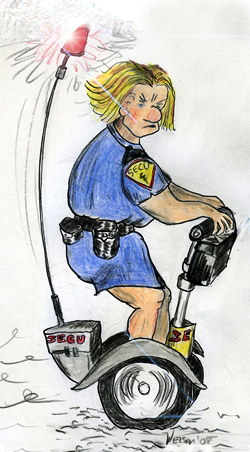
\includegraphics[height=60mm]{corps/chapitre8/img/personnage-marie-odile.jpg}
\end{floatingfigure}

C’est ainsi, étrange rebondissement, que Marie-Odile Tremblay, la Bitch elle-même, arrive, deux minutes plus tard, sur un Saguewanish orné d’un phare gyroscopique brandi à bout de tige. Dès lors, c’est le syndiqué qui explique la situation, en ajoutant que Timothée ne peut plus rouler, qu’il en a assez de ces vexations gratuites et qu’il a vraiment envie de porter plainte.

Sérieuse comme une statue médiévale, Marie-Odile fait méticuleusement le tour de la voiture sinistrée, entre un crayon dans les trous pratiqués aux pneus de droite, enregistre un clip vidéo et dicte quelques notes à sa boucle d’oreille.

- On va la faire remorquer au garage que vous voulez, dit-elle, et, de là, vous pourrez vous en occuper.

Le CS-1 accepte et l’opération est organisée illico. Que va-t-il faire maintenant ? Il est presque 17 h et son père l’attend.

Elle l’a vu regarder sa montre.

- Pour moi aussi, c’est l’heure; je viens de finir mon quart de travail.

- Ah …

- Je peux vous … te déposer où tu veux; mon auto est juste là !

En temps normal, Timothée n’en aurait cru ni ses yeux, ni ses oreilles. Il aurait plutôt estimé avoir gagné à la loterie. Mais cette après-midi, plus rien ne l’étonne. Il est devenu un brin d’herbe que le vent emporte à sa guise. Il n’a plus prise sur cette réalité si laide. Sa mère, le docteur Gagnon, Louis-Marc Richard, Dart Vader, Flipper Dauphin, le DG, Marcovsky, Bérubé, le Gros Lavoie, le père Jean, sa Saguewanish, ses pneus ! Comment supporter sans craquer autant de mauvaises nouvelles, de désagréments, de haine, de drames ?

D’un signe de tête, sans même esquisser un sourire, les yeux presque invisibles derrière ses épaisses lunettes, il accepte l’offre. Alors, contre toute attente, Marie-Odile l’informe qu’elle va le déposer chez lui à Nazareth. Autant en emporte le vent ! Incapable de parler, il acquiesce d’un geste imperceptible. Le regard vers la droite, il semble contempler la carte postale formée de l’île Saint-Barnabé, du fleuve et du contrefort de Nazareth et il semble porter attention aux nombreux marcheurs sur la promenade venus profiter de la chaude brise de ce juillet inoubliable.

À moins, suppute la bonne samaritaine, qu’il ne soit simplement perdu dans ses pensées pleines images d’holotar récitant des vers, la main sur le cœur et un genou à terre.

Chimère qui ne tient pas la route.

- Merci, finit-il par lui dire. Faut m’excuser. J’en ai plein le casque ces temps-ci et des histoires de sabotage comme il vient de m’arriver, ça devient plus dur à accepter qu’à l’ordinaire.

Elle lui répond le comprendre.

- C’est ta maison ?

Il fait signe que oui.

- Tu dois avoir une belle vue.

Sans plus parler, ils se saluent et il descend de l’auto-patrouille électrique. De sa fenêtre, Louis-Marc Richard a légèrement écarté le rideau pour mieux voir. Comme la voiture disparaît, les jappements de Gazou parviennent aux oreilles de Timothée.

- Bienvenu en enfer, se dit-il.
\chapitre{Aussi bien invoquer Quetzalcoatl, du vendredi 22 au dimanche 24 juillet 2033 }{Quand on n’a ni voiture pour se rendre au travail, }{ni Saguewanish pour circuler à l’interne, pourquoi devrait-on avoir accès aux services de télécoms ? N’est-il pas établi que les situations désagréables tendent toujours à proliférer, à s’organiser en bandes, à se concerter dans une surenchère éprouvante, à tout faire en leur pouvoir pour châtier lourdement, allez savoir pourquoi, la personne sur qui elles s’acharnent ? N’est-il pas documenté hors contestation que les objets inertes, les plus sournois étant ceux qu’on a gavés d’électronique, font généralement front commun pour nuire avec délectation aux humains, pour leur manifester toute la haine dont ils sont prodigues, pour tenter de les amener le plus douloureusement possible à leur perte ?  }

Surtout les êtres qu’ils détectent - ils en sont capables - comme étant accablés de problèmes intimes, familiaux et professionnels. On jurerait qu’ils disposent de capteurs évolués pour les repérer et les torturer encore plus cruellement. À preuve, quand Timothée a démarré une session musicale chez lui, tout à l’heure, son système lui a inopinément fait jouer un solo de trombone.

Ainsi, en arrivant au Centre, il constate que son dispositif personnel polyvalent (DPP), sa boucle d’oreille, ne fonctionne plus. Il l’a pourtant rechargé la veille, mais ce matin, le bidule semble avoir passé l’arme à gauche, probablement en ricanant. Qu’y a-t-il d’étonnant à cela ? Le gadget idiot ne fait que démontrer sa solidarité avec la franc-maçonnerie électronique encadrant la vie au XXIe siècle. Reste que Timothée a peine à refréner une violente pulsion l’incitant à aplatir le petit appareil à grands coups de talon.

De la cafétéria, Shimoune Saint-Pierre le salue de la main. Il a les yeux cernés, les traits terriblement tirés, mais il affiche un sourire qui en dit long sur l’aspect dissolu qui, de toute évidence, a caractérisé sa nuit. Timothée lui retourne un vague signe à peine esquissé et file directement jusqu’au 5e. En route, aucune rencontre détestable n’est à signaler et il ne croise pas Luce Morency. De plus, les gars du frigo n’ont pas l’air d’être en train de s’affairer sur son étage, les joueurs de 500 qui le voient passer ne l’affligent d’aucunes remarques et personne ne traîne au poste de garde. Dart Vader, lui, qui est dans la geôle du sous-sol, n’est pas là pour l’achaler avec ses histoires de nourriture. Quant à Jean Saint-Gelais, il ne semble pas rôder dans les couloirs; tant mieux. Par contre, arrivé au coqueron qui lui sert de bureau, il grimace devant l’impressionnante liste des appels à retourner : l’atelier mécanique, Robespierre, la secrétaire de Carl Michaud, le garage, Claude Sey et Marie-Odile Tremblay. Et sa boucle d’oreille est foutue. Qu’à cela ne tienne, il s’en remettra à son terminal. Moins pratique, absolument pas mobile, mais tout aussi efficace !

Le mécanicien lui apprend d’abord que sa Saguewanish a été sabotée, qu’il a fait un rapport et qu’il y aura enquête. Dès qu’il recevra le feu vert, il changera le bloc-moteur au complet; il a un «reconditionné» en stock. Mais en attendant, il ne peut pas lui prêter une bécane «de courtoisie», il n’en a plus depuis belle lurette. Désolé ! Faut se plaindre à la direction générale. Ensuite, Robespierre, le colosse au nez fourré partout, veut lui présenter quelqu’un, ou, plutôt, quelqu’une. C’est très important et le plus tôt sera le mieux. Une nouvelle histoire de Pétépano ? Quant à la secrétaire du DG, elle lui annonce la visite imminente de son patron ce matin même. Viendra-t-il avec des chiens mangeurs d’hommes, ou pire, avec Dauphin et ses Papyblues ? À son tour, le garagiste explique lui avoir changé ses pneus, mais une fois juché sur le monte-charge, le bazou a révélé que le réservoir à essence était pourri, qu’il coulait et qu’on devait le réparer d’urgence. Le problème était de dénicher la pièce de remplacement quelque part, ce qui, compte tenu de l’âge de la bagnole, n’était pas de la tarte. Il fallait prévoir plusieurs jours, peut-être même plus d’une semaine. Pour sa part, Claude Sey lui rappelle que le Flipper s’activait de plus en plus et qu’il avait désormais le docteur Gagnon dans son collimateur. De quoi tourner les talons et fuir dans le premier bar venu.

- Nous n’avons aucune trace numérisée des malfaiteurs, lui confirme Marie-Odile en fin de retour d’appels. Et puisque des pneumatiques, ça ne se crève pas par miracle et que l’homme invisible n’existe qu’au cinéma du siècle dernier, on a conclu que des gens avaient utilisé une carabine à gros plombs. Ça se vend dans les Wal-Mart. Ils ont dû s’arrêter sur la voie publique et, sans avoir peur de se faire filmer, ont tiré sur tes pneus. Va donc falloir que tu cesses de te stationner aussi près de la rue.

- Mais y pas d’autre place. Mon char est à essence …

- C’est vrai, désolée !

- De toute façon, je risque de ne plus avoir de char pour un bon bout de temps.

Il lui raconte son histoire de réservoir, puis déborde sur sa Saguewanish dont le bris criminel a probablement dû passer par le bureau de l’agente de sécurité. Elle lui demande s’il a des doutes sur le ou les coupables, ce à quoi il réplique par la négative, sauvant la mise du père Jean à qui, dans sa tête agitée, il entend régler le compte lui-même. Elle se dit intriguée par le fait qu’il est ainsi ciblé. Il lui répond que cet état de fait est probablement dû à sa personnalité marginale. Les gens voyagent en bancs de poissons, soutient-il, et si un individu semble suivre à côté du banc, certains, les éléments les plus méchants et, en même temps, les plus grégaires, en ressentent de l’agressivité et la manifestent. Parfois directement, mais la plupart du temps de façon hypocrite.

Marie-Odile sait de quoi il parle ! Elle le comprend parfaitement. N’est-elle pas elle-même «marginale» ?

- Je suis un peu forte des hanches, mon visage ne correspond pas aux canons de la beauté et en plus, je suis une agente de sécurité, une flic qui fait souvent des jobs de flic.

Pas besoin d’avoir de l’expérience ès bagatelle pour savoir que la Bitch ne semble plus vouloir agir comme son nom le laisse entendre. Même que, constate Timothée, elle vient de lui ouvrir une porte assez grande pour qu’en sorte et disparaisse tout l’Afrika Korps, cette légendaire armée du 3e Reich à laquelle appartient Hans le feldwebel SS, holotar botté et casqué présentement sur la glace. Elle lui a ouvert une porte assez grande pour qu’il y entre, lui le fils qui n’en peut plus, sans qu’il ne risque de se cogner l’ego ou de s’écorcher les sentiments. Si le ciel existe et s’il y a des saints, et si les saints ont déjà été des hommes, c’est maintenant qu’il faut qu’il y en ait un qui se manifeste pour aider l’inexpérimenté Timothée à saisir l’occasion au vol.

- Je pense que tu es injuste et dure avec toi. Mais moi, par contre, je n’ai rien pour moi.

Le «ben voyons» qu’elle lui répond constitue une sorte d’indication qu’elle pourrait ne pas le croire aussi moche qu’il semble vouloir le dire. Pour l’instant, il demeure en lice, mais la victoire n’est pas encore acquise. Il ne lui faut surtout pas en rester là; il manque au moins un point pour accéder à une partie gratuite. Timothée pour qui l’acte de séduction est une notion extravagante et inconnue, va devoir tenter la botte, la finale, celle de Jarnac. Bien entendu, son cœur s’est arrêté de battre et sa respiration ressemble à un moteur traditionnel dont l’alimentation en essence est infiltrée d’eau. Beaucoup plus tard, quand il se remémorera l’histoire, il comparera cet instant à celui vécu par un héros démineur qui, dans un film américain, à deux secondes d’une méga explosion qui aurait emporté quinze gratte-ciel, choisit de couper le fil vert alors que son camarade lui hurle de sectionner le rouge. Et ça marche !

\begin{floatingfigure}[l]{60mm}
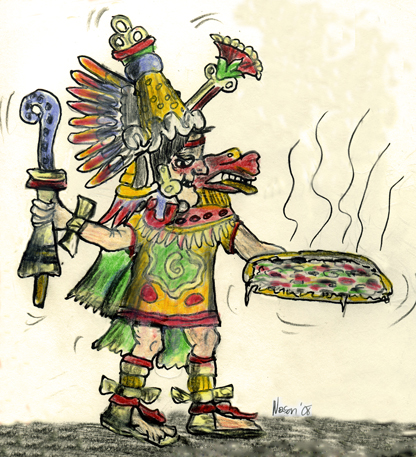
\includegraphics[height=60mm]{corps/chapitre9/img/personnage-qz.jpg}
\end{floatingfigure}

- As-tu déjà goûté à la pizza mexicaine de Da Peperone ?

Après une courte hésitation, peut-être due à son étonnement, elle répond par la négative. Timothée qui se traite de con, poursuit, axphysié par l’angoisse, dans la même foulée, convaincu qu’il est en train de couler à pic au-dessus du Triangle des Bermudes.

- Je vais en manger une à midi… euh !

Silence à l’autre bout de la connexion.

- Une spécial Quetzalcoatl …

Mais quel sinistre con ! Et si elle lui rétorque qu’elle n’en a rien à foutre de ses petites habitudes du midi ? Ou si elle lui demande pourquoi il mange aussi mal ? Ou si elle lui dit qu’elle ne veut pas s’empoisonner avec ce quetzal coa machin ? Que va-t-il pouvoir répondre ?

- Une spécial quoi ?

- Euh … Quetzalcoatl. C’est un dieu, un serpent à plumes, chez les Mayas et les Aztèques, au Yucatan, au Mexique, euh … au Guatemala.

Que c’est mal engagé, que c’est mal engagé ! Pourtant, incrédule, il l’entend finir cette essentielle question qu’il n’a pas osé compléter.

- Tu me dis ça parce que tu souhaites que je t’accompagne ?

Elle lui a tendu une perche au plus profond de sa connerie.

- Oui.

Elle lui répond trouver la perspective intéressante et qu’elle voudrait bien y aller. Mais au même moment, on frappe à la porte de Timothée.

- Excuse-moi, j’ai quelqu’un … euh, on se retrouve là-bas ? Sur l’heure du lunch ?

- Je peux y être vers midi et quart.

- OK ! euh … merci ! À tantôt !

Carl Michaud vient d’entrer dans l’officine du chef de section. Il est seul comme un roi en goguette.

- Comment allez-vous, Monsieur Tardif ?

Timothée réalise qu’il n’a pas prévenu le père Asselin de cette visite du grand patron. Mais le vieillard étant assez ouvert, il ne devrait pas y avoir de difficultés, du moins l’espère-t-il. Et si le bonhomme en dit trop, s’il s’aliène le DG ? Si Michaud recherche seulement un prétexte grabataire pour saquer l’irrespectueux CS-1 ? D’un autre côté, cette visite peut chambouler la misérable vie du vieil informaticien. Par exemple, Michaud peut lui octroyer un droit à la résurrection et Asselin peut se retrouver pris en charge, soigné, redevenu utile.

- C’est par ici, monsieur. Suivez-moi, s’il vous plaît.

- Vous êtes à pied ?

- Ma Saguewanish a rendu l’âme. Le plus drôle, c’est que monsieur Asselin, l’ingénieur que nous allons visiter, m’avait prédit, au kilomètre près, le moment où ça arriverait.

Michaud fait comme si cela ne le concernait pas.

La salle 3P-M sent particulièrement mauvais ce matin et les deux visiteurs ont peine à contenir un réflexe de recul en entrant. Deux bénéficiaires alitées semblent agitées et une tend le bras vers le grabat d’Asselin. Comme le constate Timothée, il a ses écouteurs sur les oreilles, mais Tchekhov ne joue plus, le bidule s’est complètement déchargé. De toute façon, le bonhomme s’en fiche, il est mort.

- Et merde, s’exclame le chef de section.

Carl Michaud s’approche, regarde et sans demander son reste, sans un mot pour son employé, disparaît vers son étage climatisé où la senteur de la mort n’est qu’une théorie sur papier.

Consterné, Timothée lorgne le vieil ingénieur et lui enlève le petit casque d’écoute. Puis, il lui replace délicatement les cheveux, tente de lui joindre les mains, ce qui s’avère impossible, et lui remonte le drap jusqu’au menton. Après un moment de recueillement, il quitte la pièce le cœur gros. Privé de sa boucle d’oreille, il doit se rendre au poste de garde pour enclencher la procédure nécessaire. Or, c’est sur Bérubé qu’il tombe.

- Michel Asselin est mort cette nuit. Peux-tu aller commencer ce qu’il faut faire pendant que j’avise le frigo et l’hébergement ?

- J’ai pas ben l’temps, Motté, faut que j’m’occupe des trois bénévoles qu’on nous envoie à matin !

- Laurent, je t’ai pas dit de t’occuper des bénévoles, mais d’aller vider le tiroir de monsieur Asselin, de ramasser ses affaires, incluant ses papiers et m’amener tout ça ici. As-tu compris, câlisse ?

Le préposé qui note le «câlisse» identique à celui de la veille, juge à propos d’obéir et il file vers la salle 3P-M. Dans son bureau, Timothée avertit d’abord «les gars du sac noir» puis il appelle chez Lemoignan, le salaud responsable de l’hébergement. C’est l’adjointe administrative qui répond et qui s’étonne quand elle entend l’objet de l’appel.

- Ça fonctionne l’informatique à matin, tu peux faire ton rapport directo. En passant, occupe-toi donc de tes deux autres morts, pour une fois que ça marche !

- Écoute, j’ai pas grand temps et, surtout, j’ai pas le cœur à ça !

- Là, mon beau Motté, c’est ton problème ! Veux-tu que Jean-Pascal te rappelle ?

- Non.

- Il avait de la famille ?

- Des sans-cœur qui l’ont dépossédé.

- Faut quand même que je les avise. Méchant début de journée. J’ai une moyenne de deux morts par étage à matin. On dirait qu’ils se sont tous donné le mot pour péter au frette.

Le CS-1 raccroche. Le système informatique fonctionne comme s’il s’agissait d’un symbole imaginé en l’honneur de Michel Asselin, 1951 – 2033, informaticien-choc décédé pour cause de privations existentielles.

- Maudite époque de marde, fait-il à son terminal.

Comme Bérubé est revenu avec les quelques possessions du vieillard, Timothée les lui fait enfouir dans le grand sac réglementaire, incluant le petit gadget audio. Puis, sans rien attendre de son subalterne, il s’en retourne vers la dépouille se recueillir au pied du lit dans l’attente des employés de la morgue.

- T’as une minute ?

C’est Robespierre qui vient d’entrer dans la salle. Apercevant le cadavre, il s’approche doucement.

- Ton monsieur d’informatique ?

- Oui.

- Dommage. Je peux te parler ?

- Non.

- Pas grave. Je vais t’accrocher plus tard.

Le corps parti, Bérubé revient pour s’occuper du lit et Timothée regagne son bureau où patientent les trois bénévoles. Il a tôt fait de leur distribuer des tâches et va prendre place devant son terminal. Pas pour travailler, pour ruminer son sort, pour faire le point, pour réfléchir sur le fait que son domicile est devenu une souricière où de gros minets sont à la veille de lui payer une visite qu’il ne pourra empêcher, que son travail est désormais un cauchemar plein de monstres dont l’inhumanité est proportionnelle à leur rang dans la hiérarchie, que sa vie personnelle est plus pitoyable de jour en jour, que ses chances d’être heureux sont nulles, que ses ressources financières se sont volatilisées et que son espérance en une certaine qualité de vie n’est plus. Pire, il doit tout à l’heure aller faire le beau, tâche dont il ne connaît ni l’alpha, ni l’oméga, devant quelqu’un qui pourrait, quelque part, éventuellement, dixit Shimoune Saint-Pierre, être un début de clé vers la grande console à lumières dont son existence aurait un immense besoin. Pour parler en euphémisme ! Pour réagir à cette panoplie épouvantable d’ennuis et de désagréments assortis, il n’a d’autre choix que de se dresser. Il est tenu de tout affronter en héros résigné ! Debout sur la proue, près de l’étrave, face au crachin de l’Atlantique Nord. «Je t’aurai Moby Dick !» Sa mère n’a plus que lui pour survivre. Même chose, sûrement, pour son père. Si le fils binoclard, pansu, chauvasse, puceau et équipé d’un prénom que ridiculise sa nature de nono, de raté qui ne pourra jamais rajouter de cordes à un outil d’expression qui le fera passer à l’histoire, bref si ce concentré de mocheté laisse tomber, ils mourront. Pour le moins ! Voilà quand même un incitatif de taille pour qu’il cesse de s’apitoyer sur son petit sort tata, non ?

C’est dans cet état de lucidité qu’il entreprend la préparation de ses rapports de décès. Trois morts, trois places libérées, trois nouveaux occupants, trois nouveaux fichiers, trois nouveaux jeux de peines, d’angoisse, de détresse.

- Chef, j’ai un bout de papier pour toi !

Timothée se retourne et aperçoit le visage pétant de santé de Solange Gadoury. Un instant, il songe à lui interdire l’accès à son bureau. Mais il n’en a pas le temps. La grassouillette matrone est déjà à côté de lui.

- Tape ce code quand ça t’adonnera et les 642 piastres d’avant-hier du père Lafrance vont entrer dans ton compte !

- Ça n’a pas de bon sens, madame Gadoury. Votre protégé est très malade. Il emplit ses couches aux heures. Au moins, aux heures ! J’ai personne qui veut s’en occuper. Son cas est rendu trop lourd.

- 642 belles piastres, chef !

Que dirait la Maririou ? Sûrement quelque chose comme «arrête de niaiser et fais ce qu’il faut pour ramasser ce bel argent; on en a besoin !»

- Attendez-moi ici, madame Gadoury, j’ai peut-être une idée.

Un coup d’œil à sa montre et il file vers le salon communautaire où vivote la faune habituelle.

- Monsieur Jean, j’ai affaire à vous, dit-il au bonhomme qui vient d’annoncer huit cœurs.

- J’suis pas mal occupé, mon Motté.

- Dans ce cas-là, j’vais vous parler devant tout le monde.

- OK, mais fais ça vite.

Timothée qui s’est approché de la table, entreprend d’enferrer le vieux malfrat de cette voix douce, calme, presque basse, qui le caractérise.

- Le moteur de ma bécane a sauté et la réparation va coûter au-dessus de 2 500 \$.

- Que c’est que tu veux que ça me fasse ?

- Étant donné qu’elle a été habilement sabotée, ils ont décidé de faire une enquête. Et ils vont finir par savoir que vous êtes technicien Saguewanish certifié. En plus, il y a sûrement quelques-uns de vos amis qui vont leur bavasser que c’est vous le coupable. S’ils me l’ont colporté à moi, vos bons amis, ils vont probablement en faire autant avec les flics. Autrement dit, vous êtes dans la grosse misère. Le vandalisme sur le bien public est un acte hautement répréhensible prévu dans le Code criminel. N’importe quel juge va vous condamner.

La perfidie vient de se trouver une nouvelle icône. Plus personne ne parle, ni ne fait de bruit.

- T’es malade, le Motté, finit par rétorquer le bonhomme. Tu m’accuses sans preuve. C’est qui qui t’a dit que c’était moi ? Hein ? Nomme-le ‘sti !

- On se reparlera de ma maladie, de mes preuves et de mes sources dans quelques jours quand ils vous auront coincé et descendu finir vos jours au sous-sol. Mais, d’un autre côté …

Timothée hésite et ne semble pas vouloir continuer sa phrase. Au fond de la pièce, madame Bellow sourit dans son livre.

- De quoi ?

- Ben je peux m’arranger pour qu’ils vous foutent la paix, ment-il. Il vous suffirait d’être gentil.

- Que c’est que tu veux dire ?

- Pas grand-chose. Juste de vous occuper du père Lafrance. Il en a plus pour longtemps.

- M’en occuper ?

- Oui, à chaque jour à partir de 16 heures pour le reste de la semaine, je n‘ai plus de bénévoles. Vous lui tenez compagnie jusqu’à ce qu’il soit bien parti pour sa nuit, vers 21 heures. Entre autres, ça veut dire de lui changer ses couches à toutes les heures. Si la police vient pour vous ramasser, je pourrai leur expliquer que je ne peux me passer de votre dévouement, que je n’ai personne pour vous remplacer, que vous êtes la gentillesse même, que vous êtes un intervenant bénévole exemplaire et que, dans le fond, ma Saguewanish, vous l’avez bricolée pas pour commettre un crime, mais pour me taquiner puisqu’on est de bons copains.

- Y en est pas question !

- OK. Une fois au sous-sol, vous saluerez Dart Vader de ma part !

Et le Timothée de quitter le salon. Jean met cinq courtes secondes pour réagir.

- Eh, minute ! On peut en discuter, non ?

- Y rien à discuter, monsieur Jean. Vous aidez votre ami Lafrance, ou vous ne l’aidez pas. C’est tout.

- Astie de chien sale ! Je commence quand ?

- Aujourd’hui. Suivez-moi.

Au poste de garde, ce Timothée «nouveau genre» présente la situation à Mérovée et lui demande de préparer «ce bénévole inspiré» qui entre en fonction l’après-midi même. Heureusement que les verres du vieillard sont aussi épais, sinon l’intensité de la haine que le CS-1 y discerne le fustigerait sur place.

Et c’est presque en souriant qu’il s’en retourne à son bureau expliquer le rebondissement à Solange Gadoury. Alors, la conscience tranquille, il accepte le petit papier. Et puis pourquoi ne l’aurait-il pas fait ? 642 \$ quand on est moribond et sans succession, ce n’est rien. Mais 642 \$ quand on nage dans les ennuis, ça permet de se garder le nez hors de la vase deux ou trois jours de plus.

Peu après, Timothée est chez Da Peperone, assis sur le bout des fesses en face de Marie-Odile. Comme c’est la coutume sur l’heure du midi, l’établissement a fait le plein avec des cols bleus, la voirie municipale occupant un grand terrain deux rues plus au sud, avec des travailleurs du complexe commercial qui s’étire de l’autre côté de la chaussée, avec du personnel du Centre régional pour les personnes handicapées intellectuelles, le C2R2HI, dont on aperçoit la sinistre construction de la fenêtre du resto et, malheureusement pour l’agente de sécurité et le chef de section, par des employés du CRG-BSL dont l’édifice est à deux pas. C’est ce qui explique que leur inoffensif rendez-vous, repris sous forme de médisance croustillante, déferle partout au Centre à la vitesse de l’éclair. Tellement que même Shimoune absorbé dans sa distribution de manger mou, en apprend une variante : «Apparemment, la Bitch se fait sauter par le Motté».

Autour d’une «médium Spécial Quetzalcoatl» avec «extra piments forts», on parle d’abord des déboires de Timothée, de certains déboires s’entend, soit de sa boucle d’oreille qu’il devra remplacer, de sa voiture qui est en réparation et de sa Saguewanish qu’on soupçonne d’avoir été sabotée. Telle que présentée, l’histoire arrive même à dérider Marie-Odile. Évidemment, Timothée se garde bien de mentionner le père Jean. Peut-il faire confiance à cette femme flic ? En fait, il parle très peu. Puisqu’il craint de passer pour idiot, puisqu’il est gêné et empêtré dans son langage corporel empoté, il ne fait qu’exacerber son absence naturelle d’éloquence. Heureusement, Marie-Odile compense. Elle a la jactance nerveuse. Elle papote. Elle jacasse pour combler le vide. Elle dérape même sur les mièvreries. Et la voilà qui livre quelques pages bien senties sur son boulot, ce qui n’a rien d’étonnant, les gens étant ainsi faits. Puis, au terme d’une rapide transition qui recalerait un étudiant au bac, elle déborde sur sa vie personnelle, une vie ennuyante, semble-t-il, où rien n’arrive jamais. Pas de sorties théâtre ou ciné, jamais de soirées au restaurant, il y a au moins dix ans qu’elle n’a pas voyagé et elle ne pratique plus de sport. Ça commence à paraître et elle est à la veille de faire quelque chose. Mais elle ne sait trop par quel bout prendre cela. Ses seuls loisirs sont le ciné-maison et Internet. Pas un mot sur Ilsa la louve des SS.

Et pour cause, elle s’occupe de ses parents qu’elle visite presque tous les jours, deux braves vieillards encore aptes à se débrouiller qui viennent d’atteindre 79 ans et qui sont sans le sou. Ils ne gagnent plus suffisamment pour vivre de façon autonome et Marie-Odile doit leur consacrer une partie de ses revenus. C’est son père le pire, explique-t-elle. En raison de l’usure générale de son corps, il ne peut plus exercer son métier de serveur. L’arthrite et les maux de dos ont fait leur œuvre. De plus, c’est un vieux noceur qu’elle-même se trouve incapable de gérer; le bonhomme est imprévisible, un «loose cannon » comme disent les Montréalais. Quant à leur bungalow, il date de 1967 et est en très mauvaise condition. Le pire c’est qu’il est hypothéqué jusqu’au trognon. Bref, elle craint pour eux s’ils se retrouvent «placés» au CRG-BSL. La loi du Gros Turcotte est implacable : dès qu’on coûte plus cher qu’on rapporte, on est «pris en charge». Il faut travailler dans une telle institution pour avoir, n’est-ce pas, une très bonne idée de ce qui pourrait trop rapidement leur arriver. Mais, bon, a-t-on le choix ? Tout cela l’angoisse terriblement.

Dès lors, tous les ingrédients sont en place pour que survienne la question tant redoutée.

- Et toi, ton père, ta mère ?

Ce qu’il ressent alors pourrait être classé comme étant un arrêt cardio-respiratoire. Sauf qu’il est conscient de l’énorme bêtise qu’il a commise en s’imaginant pouvoir amadouer et manipuler cette femme qu’on lui a présentée comme étant la «clé» de sa survie. Il est hors de question qu’elle apprenne comment il s’occupe, lui, de ses parents. Elle est flic. Elle va le traîner à coup sûr jusqu’à la guillotine ou la chaise électrique la plus près du CRG. Puis, devant une populace haineuse, lanceuse de tomates avariées, de crottin mou et de cailloux, elle se fera aller le bras séculier. Ce sera Schlac!, ou Zap!, selon le cas. Timothée sait une chose : même si son silence s’inscrit dans son comportement général, celui adopté en début du Spécial Quetzalcoatl extra piments forts, il lui faut réagir. Impérativement réagir. Il doit triompher de ce redoutable écueil. Le reste de sa vie en dépend. Mais en même temps, il ne peut répondre à une telle question. Comment le pourrait-il ? Sauf que s’il ne dit rien de valable, tout est foutu ! Il n’a d’autre choix que de redémarrer la machine. Sans erreur possible !

Ainsi, il la regarde et se lance dans le vide.

- C’est moi le joueur derrière cet holotar qui se prend pour Roméo et qui s’est amouraché d’une Juliette esthétiquement remaniée, un holotar que je soupçonne d’être à toi.

Elle le fixe d’abord sans expression, comme si ses yeux étaient devenus deux scanneurs de haute précision. Puis, quelques instants plus tard, elle les illumine d’un sourire qui pourrait la faire passer pour belle.

- Je m’en doutais bien.

L’étape suivante est cruciale. Les représentants commerciaux l’appellent «closing» et les Français, «emballage de la nana». Il s’agit maintenant de consolider les acquis, de les transformer en quelque chose de définitif, de momentanément ou de temporairement définitif. Que dire ? S’essayer avec un poncif hollywoodien comme «on va chez toi ou tu viens chez moi, bébé ?» Timothée est complètement démuni. Démuni comme un coq à viande miraculeusement échappé d’une des mille cages d’un camion en route pour l’abattoir et qui se retrouve dans un poulailler plein de grosses poules lourdement expérimentées. Il faut se rappeler que c’est la première fois de sa vie que le fils de la Maririou travaille une femme au corps.

C’est Marie-Odile que l’on ne dirait guère mieux outillée, qui attaque pourtant, toute chattemite.

- Penses-tu qu’on va continuer à jouer à Roméo et Juliette avec nos holotars ?
Il fixe le reste de pizza tellement la question est insupportable. Quetzalcoatl, dieu de Da Peperone et des Mayas, serpent à plumes à qui on doit la perte de Moctezuma, fais quelque chose, sacrament ! Aide-moi à me tirer de ce merdier !

- Ben, euh …

- Ben, j’sais pas, moi, à c’t heure qu’on se connaît ….

- Euh … c’est vrai qu’on pourrait se passer de machines pour un bout de temps …

- Ouin !

Un silence gênant vient les éprouver. C’est la serveuse qui casse la glace en s’informant s’ils ont aimé la pizza. Tous deux opinent du chef en se zieutant du coin de l’œil. Dans sa tête, Timothée entend une sorte de mantra l’amener tranquillement vers la folie: «faut closer», «faut closer», «faut closer» ! Il revoit ce lieutenant parachutiste crier «Go go !» à ses GI qui se précipitent un à un en dehors de l’avion. Il fonce.

- Euh, ça te tenterait-tu qu’on remette ça ?

Encore une fois, ses yeux viennent s’illuminer et elle redevient belle.

- Ouin, ça serait le fun, quand ?

Quetzalcoatl, à l’aide ! Je me meurs !

- Euh … je sais pas, ce soir ?

Elle sourit davantage. Timothée est encouragé. Ça marche, sacrament !

- Euh … on pourrait aller Au Vieux Cormier, ils ont du pas pire manger et ils sont pas chers …

- C’est vrai, j’aime ça c’t endroit-là, ment-elle.

Toc-schloc toc-schloc toc-schloc, fait son pauvre cœur.

- À quelle heure ?

- B’en j’sais pas, euh, 19 heures ?

- OK, j’vas être là !

Pas croyable ! C’est gagné. Jamais il n’a été aussi fier de lui, le Timothée-Milet, une femme vient de lui dire oui ! À lui ! Il a fait ce qu’il devait et ça a marché. Mais il ne s’agit pas de n’importe quelle femme. C’est la Tremblay, une flic, la clé potentielle d’un début de solution.

Méprisant les petits regards mesquins, les éclats furtifs de rire hypocrites, tous deux réintègrent leurs locaux au CRG, elle au 2e, lui au 5e. Si avant de prendre l’ascenseur il a dû saluer l’inquiétant docteur Bellavance qui l’a gratifié d’un «comment allez-vous, monsieur Tardif», en le quittant, il aperçoit Mme Thériault et Mme Labbé entrer furtivement dans le salon communautaire. L’idylle semble durer, pense-t-il. Mais il a bien d’autres soucis en tête et ces deux vilaines mémères ne font pas le poids : ce soir il lui faut absolument en arriver au sens ultime de l’expression «devenir un homme». Cela, sans Petepano, se dit-il, en voyant Robespierre lui faire signe.

- J’ai quelqu’un à te présenter, lui répète le désœuvré permanent. Une madame Martin qui veut te parler sans faute.

- C’est qui ?

- Une infirmière, quelqu’un dans mon cercle d’amis.

- Elle me veut quoi ?

- Pas de mes oignons. Mais je la connais assez pour savoir que c’est sérieux.
Béatrice Martin était une idéaliste dans la jeune quarantaine qui, pendant une quinzaine d’années, avait tenu un dispensaire en Haïti. Depuis six mois, elle était de retour à Rimouski, malade et épuisée, et, par un hasard de circonstance, avait fraternisé platoniquement avec Robespierre, «le plus grand cœur de ce côté-ci du fleuve». Or, hier soir, dans le cadre d’un mini cocktail entre copains, elle avait posé des questions sur Timothée, un Tardif qui pourrait être le fils de Marie Rioux, la fille d’une amie très chère de sa grand-mère. Puisque cette Rioux avait naguère épousé un certain Romain Tardif et qu’ils avaient eu un garçon appelé Timothée, un nom quand même rare, elle se demandait si ce compagnon de travail de Robespierre pouvait, par le plus grand des hasards, être apparenté à cette Marie. Si cela était possible, elle avait un document de première importance à lui remettre.

- Elle a su comment que toi et moi étions collègues ?

- Je racontais comment le personnel du CRG était baveux, méchant, désagréable, arrogant, bref, chiant auprès des vieux. Alors, j’ai parlé de toi comme étant un cas unique faisant tout le contraire. Et c’est en nommant ton nom qu’elle a réagi. Elle nous attend dimanche après-midi chez elle. Je passe te prendre ?

- J’ai plus de char !

Robespierre tourne les talons.

- Fais attention à toi, mon ami.

Quelques heures plus tard, Au Vieux Cormier, tout va se dérouler comme dans un film à l’eau de rose, comme dans un roman où le pathos se transvase au kilo, comme dans un soap californien où l’héroïne siliconée sur le retour fait semblant de ne pas trouver cucul la passe de son Casanova de banlieue, bref, comme dans une vie imaginée par ceux qui n’en ont pas. Les dialogues seront lamentables, les premiers sourires tendus et les manières de table ampoulées. Quant aux épanchements, ils nécessiteront une bouteille de pinot noir estrien avant de pouvoir démarrer. Mais dès ce moment, ce sera une course à la «qui perd gagne» entre ces deux êtres privés de rapports humains, pour savoir lequel des deux confiera le plus de secrets à l’autre.

Et lorsque, vers les 22 heures, ils finirent par convenir d’aller chez elle, ce fut dans un contexte épouvantable de malaise, de gêne aussi paralysante qu’une morsure de serpent mexicain - «Quetzalcoatl, aide-moi, sacrament !» - de souffrance déclencheur d’infarctus, de peur, de désir, d’angoisse et d’appétit tout entremêlés. Puis, il fallut tenir inutilement des propos vides pendant une grosse heure avant d’accéder, toc-schloc toc-schloc toc-schloc, au tabernacle du sanctuaire. Et là il fallut encore un solide quinze minutes avant que Marie-Odile n’ait le courage d’enlever l’éclairage. «Te Deum laudamus» ! En passant sous silence l’impressionnante collection de maladresses commises de part et d’autre, on peut dire que quand, aux petites heures, Timothée appela un taxi avec la boucle d’oreille de Marie-Odile, l’inévitable avait été consommé. À 43 ans, « jouez hautbois, résonnez musettes », le fils de la Maririou avait perdu son pucelage, grâce au patient vouloir d’une agente de sécurité chattemite en mal hurlant d’affection, «Chantons tous son avènement !».

Sauf qu’il le lui avait avoué. Inutilement avoué doit-on croire, puisqu’elle s’en était aperçu dès la première minute. Non pas qu’elle était une rombière expérimentée, mais, au fil de sa vie d’adulte mal lunée, elle avait acquis un peu d’expérience, le mot «peu» se référant ici à un calcul pouvant être établi sur les doigts d’une seule main.

C’était donc ça, faire l’amour, sentir un corps féminin sur soi, vibrer avec quelqu’un dans une intimité exultante, oublier, un instant, qu’on était un binoclard grassouillet à moitié chauve de qui la planète entière se moquait. Plonger, tête première, dans les entrailles chaudes, humides, sans fonds, insatiables d’une cousine, si ce n’est la petite sœur par la fesse gauche, du redoutable Quetzalcoatl, question d’y fouiner en toute liberté, les truffes du juste bonheur.

C’est ce qui explique que le lendemain, au début de l’après-midi, après s’être assuré que tout se passait normalement – un bien grand mot – chez ses parents, Timothée va, pour la première fois de sa vie, connaître la sensation de se présenter chez une dame «la bitte sous le bras». Cette fois il ne faudra que cinq minutes avant que l’on troque son babil idiot contre une session d’effusions, d’abandon et de rattrapage par rapport à leur vie cruelle.

Pourquoi fallut-il, Dieu du ciel, que ça prenne 43 ans ?

\begin{floatingfigure}[l]{40mm}
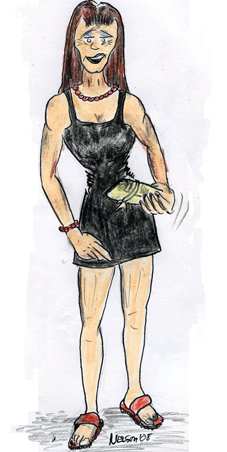
\includegraphics[height=60mm]{corps/chapitre9/img/personnage-beatrice.jpg}
\end{floatingfigure}

Béatrice Martin était une femme plus mince que menue, plus belle et attirante que sexy, que de coquines pattes d’oie avaient commencé à décorer, on aurait dit, pour le mieux. Sûre d’elle dans sa petite robe noire, elle les avait accueillis, Timothée et Robespierre, avec beaucoup de chaleur et leur avait offert de la bière. Puis, elle était rapidement passée au vif du sujet, une histoire, somme toute assez triste relative à sa grand-mère Joncas, Rose de son prénom, qui avait travaillé une bonne partie de sa vie dans un magasin de coupons de Rimouski. Or elle s’y était liée d’une grande amitié, semble-t-il, avec une nouvelle employée, Marceline Rioux, une malheureuse très amochée par la vie, qui mourut quatre ans plus tard en 1968. Sentant sa fin proche, la pauvre dame avait confié une forte enveloppe à Rose, lui faisant promettre de la remettre à sa fille advenant qu’elle décède. Mais quand cela se produisit, il ne fut pas possible d’accomplir cette ultime volonté. Retrouvée à Québec, la jeune femme refusa aussi bien le manuscrit que le signet mortuaire imprimé à la mémoire de Marceline. La bonne Rose dut redescendre, bredouille, à Rimouski. Peut-être par sentiment de culpabilité, elle conserva le document toute sa vie et, à la fin de ses jours, la laissa à sa fille, Jacinthe Martin, à qui elle raconta toute l’histoire.

- C’était ma mère. Et, je sais pas trop pourquoi, elle a choisi de ne pas s’en débarrasser. Elle l’a placée au travers de ses papiers importants, ses polices d’assurance, ses placements, etc. Quand elle est morte, le printemps dernier, j’ai commencé à faire le ménage dans sa paperasse. Dieu sait qu’il y en avait, ma mère était une ramasseuse. Mais, quelque part, ça tombait bien, j’étais en convalescence. C’est ainsi que j’ai découvert l’enveloppe. Intriguée, je l’ai ouverte et j’y ai trouvé une très longue lettre, un récit très touchant que j’ai lu sans pouvoir m’arrêter. J’en suis désolée. Mais, ç’a été un mal pour un bien, car la gravité du contenu m’a incité à vous retrouver, monsieur Tardif.

- Euh … merci madame.

- Vous êtes bien le fils de Marie Rioux dont le mari était Romain Tardif ? Des gens de Saint-Anaclet qui ont péri, me semble, aux alentours de 2027.

Que répondre ? Que ses parents ne sont pas morts, mais vivent présentement un enfer à l’autre bout de la ville, dans Nazareth ? Que lui, il est en train de devenir dingue avec cette histoire ? Qu’il se farcit une femme flic pour avoir une chance de voler des produits pharmaceutiques qui pourront acquitter une dette contractée auprès du shylock d’Esculape.

- Oui, répond-il, tandis que Robespierre corrobore de plusieurs signes de tête.
Elle lui tend une enveloppe un peu salie et jaunie, une enveloppe format lettre tellement bourrée qu’il a fallu la ficeler pour qu’elle tienne fermée.

- Alors, j’imagine que le contenu va vous prendre aux tripes.

Lentement, comme s’il présidait une cérémonie religieuse, Timothée retire la ficelle et ouvre le petit paquet. Il en extirpe une liasse de feuilles manuscrites. Sur le dessus, une page pliée en trois attire son attention. Elle est datée du lundi 27 mars 1967. Le texte est court et inquiétant :

- «Il est arriver un dramme dans la vie de Marie ma fille de 16 an et depuis ce temps la elle m’a fuit et a les devenu renfermé et tout le tant triste. Elle était déjà pas du monde mais ces devenu pire. Elle croix que cet pas à cause d’elle que j ai tuer son pére que cet juste à cause de moi que je lé pas défendu que j me suis juste vanger. SVP, quand je serai morte, remetter lui cette lettre. Je conte toute l’histoire. Merci.»

- Mon Dieu !

Timothée replace maladroitement les feuillets dans l’enveloppe.

- Euh, madame Martin, faut que j’aille lire ça à tête reposée.

- Je comprends.

- Euh … je sais pas trop comment faire pour vous remercier.

- Venez prendre un verre avec Robie (Robie ?, tiens tiens) de temps à autre. Ça va me faire plaisir.

Sans tenir compte de Gazou qui, encore une fois, veut le dévorer, Timothée s’approche de son père en train de regarder sa télé sans son, tandis que sa conjointe dort. Il lui tend la feuille pliée en trois.

- Faut que tu lises ça.

- C’est quoi ?

- Lis.

Quelques instants plus tard, les deux hommes se regardent.

- Veux-tu ben me dire c’est quoi c’t’affaire-là ?

- Faudrait lire toute la liasse pour le savoir.

Le bonhomme se lève, ce qui fait gronder le chien-rat.

- Mon Dieu Seigneur ! J’aime pas ça, c’t histoire-là. Viens, on monte chez toi, tu vas me faire la lecture, Timothée-Leary. Ici, on va déranger ta mère. J’ai de la misère avec mes yeux et c’est écrit plein de fautes avec des pattes de mouche. Mais avant, je pense que je vais mettre mon pied au cul de ce p’tit calvaire de chien lette !

Ce qu’il ne fait pas, bien entendu.

Arrivés à l’étage, ils s’installent dans le salon où, en moins d’une heure, ils vont voir défiler une histoire épouvantable, celle d’une petite victime qui, devenue adulte, continuera inutilement de l’être. Jusqu’à aujourd’hui.

- Lis mon Timothée !
\chapitre{Marceline saute une coche, le vendredi 4 mai 1962 }{A onze ans, }{une fillette pourra être agacée par plusieurs choses. Par exemple, elle pourra détester se faire traiter de Bezo, comme tous les Belzile, ceux de Léonce, qui, en soixante ans, se sont succédé sur cette terre compliquée du 3e Rang Ouest de Saint-Fabien, une terre escarpée, constellée de roches, éloignée de tout, dont la richesse en cèdres et en érables avait été bûchée à quelques reprises. Si l’improbable surnom de Bezo était resté, fixé au vernaculaire comme synonyme de «colon plein de poux », celui de Belzile était disparu. Marceline, la dernière à pouvoir le porter au fin fond de ce rang jouxtant ceux de Saint-Mathieu, s’appelait Rioux depuis douze ans, à cause du grand Edmond, ce fier-à-bras de Saint-Simon qu’elle avait fini par marier. Les autres Belzile, ses jeunes frères et sœurs, étaient tous partis s’établir à Québec sous le nom de «Belzile \& frères, électricité plomberie», les garçons étant plombiers, les filles ayant épousé des électriciens.}

C’est ainsi que par défaut, l’aînée était l’héritière des espoirs trahis du grand-père Léonce, un brave homme plus enclin au rêve qu’à l’agriculture. En ce printemps de 1962, l’héritage n’était plus qu’une terre à bois laissée à elle-même, deux vieux bâtiments à moitié défoncés et une maison en bardeaux de cèdre qu’il faudrait retaper de fond en comble, la cabane des Bezo. Marie des Bezo détestait donc son statut social, ce qui ne l’aidait pas à entretenir des rapports amicaux avec les autres gamines à l’école du rang.

\begin{floatingfigure}[l]{40mm}
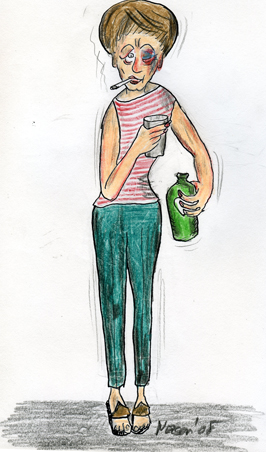
\includegraphics[height=60mm]{corps/chapitre10/img/personnage-marceline.jpg}
\end{floatingfigure}

En plus d’être ostracisée, puisque Bezo, une mouflette de onze ans pourra être exaspérée du fait d’être pointée du doigt comme étant la fille à Edmond, ce sombre bagarreur que tout le monde redoutait et dont on aimait raconter les exploits, le soir dans les chaumières, ou, pire, d’être la fille à Marceline, une assistée sociale maigre, probablement alcoolique, soupçonnée de mœurs légères que l’on apercevait occasionnellement, à l’hôtel, en compagnie des plus assoiffés noceurs du patelin. Avec sa vieille camionnette Fargo 1952, la «femme des Bezo» descendait régulièrement au village, mais parfois, elle faisait un crochet par l’hôtel. Ces jours-là, Marie devait se débrouiller seule pour le souper. Et quand sa mère revenait, avinée, bruyante et gauche, l’enfant faisait celle qui ne voulait pas l’entendre, qui ne voulait pas la voir, qui ne voulait pas l’embrasser, qui ne voulait surtout pas sentir son linge enfumé et son haleine de «fonds d’tonne». Certaines bonnes âmes avaient peine à endurer cette Bezo à la messe du dimanche accompagnée de sa petite fille. Pour ces gens, il aurait fallu qu’elle soit dénoncée en chaire et mise au ban de la communauté. Évidemment, si Edmond ne la maltraitait pas tant, colportait-on, peut-être boirait-elle moins. Mais, bon ! Heureusement que le grand tocson ne se pointait pas plus souvent le bout du nez. Marie Rioux avait donc honte de ses parents et apprenait à vivre sans avoir à ne parler à personne, en ne se préoccupant que d’elle-même, au point de se cacher de la nourriture pour être bien certaine de ne pas en manquer.

Passe encore être une paria, mais une Bezo de onze ans pourra particulièrement détester que l’on s’en prenne à son apparence. À onze ans, une gamine a de ces fiertés qui commencent à lui titiller les hormones. Marie qui, paradoxalement, marchait en tout temps la tête haute, n’hésitait jamais à regarder les gens dans les yeux, cela sans jamais sourire, et faisait constamment des miracles pour que ses vêtements aient l’air propres et neufs, abominait les visites de son père. C’est qu’en ces occasions, il lui arrivait de se ramasser quelques bonnes torgnoles qui lui déformaient parfois le visage pendant un jour ou deux. Comme résultat, les autres écoliers se moquaient plus que jamais, ce qui, chez elle, se transformait en rancœur et morgue. Heureusement, elle ne pouvait comparer sa situation avec celle de Marceline dont les traces de raclées nécessitaient souvent plusieurs semaines avant de se résorber complètement. Convaincue de ne pas mériter d’être maltraitée avec autant de méchanceté, elle s’interrogeait cependant sur sa mère au comportement général plus qu’erratique. L’ivresse n’expliquant pas toujours tout, il se pouvait que la Bezo ait poussé son Edmond à bout pour qu’il s’emportât ainsi, qu’il se mit à tout casser et à frapper ses proches. Il paraîtrait que depuis Ève et le serpent, la femme est souvent la cause de bien des débordements masculins. Donc, quand la petite saignait du nez, qu’elle avait la lèvre fendue ou la joue enflée, il se pouvait que ce soit par la faute de sa mère.

Edmond Rioux, brute dangereuse qui voyageait un peu partout au Québec pour des négociants de Montréal sévissant dans la voiture d’occasion, venait le plus rarement possible à Saint-Fabien. Et lorsqu’il se pointait, c’était la plupart du temps un vendredi en fin de soirée avec une «caisse de 24» et un «40 onces» de Bols ou de De Kuyper, ainsi qu’avec quelques billets de 20 \$ qu’il exigeait, telle une cérémoniale préivresse, qu’on lui sortît de sa poche de pantalon. Au printemps, Marie s’était retrouvée la lèvre ensanglantée pour s’être refusée à ce petit jeu. Le fier-à-bras s’installait dans la cuisine et se mettait à monologuer à voix forte sur sa vie de héros, sur ses bagarres les plus récentes, sur ses dernières trouvailles automobiles, sur ses patrons qui étaient de plus en plus voleurs et baise-la-piastre, sur René Lévesque qui avec son histoire de «nationalizâtion» de l’électricité, ”un autre mot à queue, bonyeu !”, s’était fait «r’placer les cordes vocales», ou encore sur les Canadiens qui ne savaient plus jouer au hockey tandis que les «Maple Leafs, ceuzes-là, y gâgnaient». À tout coup, il continuait son emportement sur le fait que l’eau du 3e Rang était «soufrée», qu’elle sentait les oeufs pourris, que si on «se lavait avec, on puait la charogne» et qu’elle n’était pas buvable. Ce stade franchi, il n’y avait qu’un échelon à gravir pour que sa cocotte pression n’explose. La plupart du temps, le prétexte était de nature sexuelle. Une pulsion bestiale intimait soudainement au colosse l’ordre d’exiger son dû et la Bezo devait dès lors obéir. Advenant que Marie soit dans les parages, elle était chassée avec force invectives. Puis, coincée contre le mur, Marceline subissait la virilité triomphante d’Edmond. Neuf fois sur dix, ces viols de fond de cuisine n’avaient pas de suite. Mais il arrivait qu’une grossesse s’ensuive. En ces occasions, la pauvre femme avait recours à la science d’Eugénie Jean, une bonne grand-mère catholique qui savait comment «empêcher la famille une fois le mal accompli». «Le Bon Dieu est bon, disait-elle, et Il peut pas être du bord des prêtres là-dedans !»

Dans ce monde sordide, Marie, petite fille sans jamais d’amis, s’était construite une planète à elle. Dans les fourrés autour de la maison, dans des clairières, près d’un des nombreux ruisseaux, à côté de «la grosse roche proche de la coulée», sous sa grande épinette à elle, voire sous la galerie d’en avant, elle entretenait des pièces imaginaires. Ici sa chambre de princesse d’où un beau chevalier viendrait un jour la délivrer. Là, le siège de son gouvernement. Plus loin, son salon de thé. À côté, son chalet de chasse. Puis le donjon de son château, le garde-manger de ses cuisines, son magasin de livres, sa petite chapelle du Bon Jésus et la scène d’où elle donnait ses concerts d’harmonica.

Un de ces sinistres vendredis, la gamine était alors âgée de neuf ans, son père lui avait offert une musique à bouche en lui révélant, à grand renfort de rires gras, tout ce qu’il y avait à dire :

- Tu tires p’is tu pousses, comme pôpa dans môman, p’is les notes vont jouer. Pratique-toé comme y faut, parce que quand j’vas r’venir, va falloir que tu m’jouses le «reel du mocking bird» !

Intriguée, stimulée, Marie était disparue. Dès l’aube du samedi, elle s’était aménagé une salle de concert sur une hauteur à quelques arpents de la maison et s’était mise à apprivoiser l’instrument. Il lui avait fallu une journée pour pousser «Frère Jacques», deux jours pour interpréter «Le cowboy fait le tour de la montagne» et un mois pour crachoter l’«Oiseau moqueur». Bien sûr, ses notes étaient approximatives, pleines de parasites mal discriminés, les demi-tons étaient escamotés, mais l’essentiel y était. On pouvait reconnaître les pièces qu’elle livrait. Elle eut besoin de moins d’un an pour savoir tirer le maximum de son «ruine-babines», en compensant pour certaines «notes noires» impossibles à rendre. Elle apprit à jouer tous les cantiques qu’elle connaissait, toutes les chansons qu’elle entendait à la radio, ou, quand le signal du Pic Champlain entrait assez fort dans les oreilles de lapin, à la télévision, une vieille Sylvania qui, une fois sur deux, nécessitait qu’on lui administrât un violent choc sur le côté pour fonctionner.

En partant de chez elle, Marie devait marcher près de trois kilomètres pour parvenir à l’école élémentaire, la «‘tite école» située au deuxième rang. Quand il faisait beau, le voyage était agréable et c’est en chantonnant ou en jouant de son harmonica qu’elle montait et descendait les innombrables côtes. Elle s’arrangeait cependant pour se mettre en route bien avant l’heure, question de ne rencontrer personne en chemin. Surtout les trois frères Jean-Pierre, Jean-Paul et Jean-Marc Roy. Elle les détestait tellement, eux et leur puanteur de souillon, qu’elle leur avait consacré une cérémonie. S’arrêtant devant une grosse roche à quelque 200 mètres de sa maison, elle la frappait à grands coups de trique, une «p’tite hart» comme elle le disait, à défaut de pouvoir le faire sur les garnements. C’était particulièrement vrai les jours où le plus vieux, Jean-Pierre, s’était appliqué à se faire rouler le farcin encroûtant ses bras, avec le pouce de la main opposée.

Mais s’il pleuvait ou crachotait ou poudrait, le trajet pouvait être un supplice. Elle arrivait parfois transie et Rhéa Théberge, l’institutrice, devait alors l’installer près du poêle. L’hiver, en période de grand froid, sa mère l’ayant autorisée à dormir à l’école, c’était la délectation suprême : elle s’amusait sur l’harmonium de la petite pièce qui servait d’étude à la résidente. C’est que flairant un talent certain, la jeune femme avait commencé à initier Marie à la logique musicale grâce à ce vieil instrument à vent. Encore là, Marie apprit tellement vite qu’à onze ans, elle pouvait jouer sans fausse note et avec les bons accords, une dizaine de cantiques, dont «J’engageai ma promesse au baptême», «Regarde avec amour», «Dans cette étable» et «Nouvelle agréable».

Entre elle et la demoiselle Théberge, une sorte d’entente s’était tissée. Comprenant que Marie, une enfant brillante pleine de potentiel, était molestée et laissée à elle-même, elle la prit sous sa houppe. Et plus encore. Elle la mit au fait des plaisirs de la connaissance, lui prêta des livres, des recueils et des revues. Elle l’initia au dessin, lui enseigna comment ménager ses crayons de couleur. Elle lui apprit à écrire de la musique. Elle en fit son adjointe pour assister les plus jeunes, de petits malheureux qui eurent ainsi à subir le caractère autoritaire, sec et contrôlant de la gamine. Il lui arriva même de la garder avec elle le soir, quand il faisait beau, surtout vers les fins de mois alors que chez les Bezo, il n’y avait plus grand-chose à manger. Le subterfuge pour que Marceline accepte était de dire qu’elle avait besoin de Marie, «une petite si raisonnable», pour l’aider à faire le ménage ou à rentrer du bois ou à corriger des cahiers, ce qui était parfaitement faux. Ces soirées n’étaient que prétextes à musique, l’harmonium étant poussé au maximum de son potentiel. Qui dort dîne.

Un jour, voyant la petite fille souffrir des quolibets que des enfants, dont les frères Roy, lui administraient en raison de son œil amoché, Rhéa se choqua et admonesta les galopins de sérieuse manière. Sur l’heure du midi, alors que les élèves étaient tous dehors en train de jouer, sauf peut-être les rares chanceux qui n’habitaient pas trop loin de l’école, elle essaya de faire parler Marie. Mais pas une seule parole ne put sortir tellement la boule qui lui bloquait le pharynx était énorme. Elle la prit alors dans ses bras. Après un réflexe de recul, la petite laissa la chaude affection de Mlle Théberge l’enrober et, malgré d’héroïques efforts, éclata en sanglots. Ce que voyant, l’institutrice en fit autant. S’il n’est pas exagéré de dire que toutes deux en gardèrent toujours un souvenir précis, il est surtout important de constater que, dans l’immédiat, les liens les unissant s’en retrouvèrent renforcés. Marie fit de Rhéa sa source unique de tendresse, de compréhension et de savoir. Tant pis pour Marceline qui n’osait s’adonner à de telles effusions.
S’il est vrai que chaque humain est censé connaître un «vendredi noir» au moins une fois dans le courant de sa vie, celui de Marie survint le 4 mai 1962.

Verre de gin dans une main, cigarette dans l’autre, Edmond semble de bonne humeur, assis, jambe croisée, sur le côté de la table de cuisine. Il s’est pointé, une heure plus tôt, au volant d’une Chevrolet Impala SS flambant neuve, une 350, avec sièges baquets, hard-top, carrosserie rouge et garnitures blanches. Apercevant la fillette, il lui demande de lui interpréter le «Mocking Bird» avec son harmonica. Mais comme il est particulièrement ivre et désagréable, elle refuse.

- J’t’ai dit de jouer, bonyeu !

- Laisse-moi tranquille, pleurniche-t-elle en manœuvrant pour s’échapper.

Malgré sa balourdise, il l’attrape par son tablier couvre-tout et la tire sur lui.

- Fais-y pas mal, supplie Marceline, pointant de son verre de gin.

- Toé, ta yeule !

En tentant de se libérer, Marie se met à crier, presque hystérique.

- Lâche-moi, lâche-moi, lâche-moi !

- Ah c’est comme ça que tu me remercies ?

D’une main, il la saisit par les cheveux et de l’autre, il lui fouille les poches de son couvre-tout. Comme il l’espérait, il découvre l’harmonica et, sourire en coin, la pose par terre entre ses deux souliers.

- Qu’in !

À coups répétés de talon, il écrase l’instrument qui se retrouve en débris à tout jamais perdus. Marie est épouvantée et ses hurlements atteignent l’insupportable.

- T’es méchant, méchant, méchant !

Pour toute réponse, Edmond lui allonge la gifle du siècle, ce qui propulse la gamine, la tête donnant violemment contre le mur de petites lattes.

- Décâlisse, j’veux pu te voir la face icitte !

Plus morte que vive, Marie s’en va alors se réfugier dans sa chambre, à l’étage. Même si elle sent son visage enfler, son cœur grossir, sa haine décupler, elle se couche et tente de convaincre ses grands yeux sombres de se fermer, d’oublier l’image de sa musique à bouche aplatie et en mille miettes.

En bas, le temps file. Edmond en est rendu à l’étape libidineuse et pour la énième fois, Marceline doit subir ses molestations. Pourtant, cette fois, il y a variante. L’ivresse pesant de tout son poids, la brute a fort à faire pour se placer en situation d’assouvir sa fureur bestiale. Même qu’il doit se reprendre et s’aider de la main, pour finalement renoncer, ce qui a l’heur de le mettre vraiment hors de lui.

- Bonyeu d’bonyeu, t’es aussi bandante qu’une couenne de lard !

La malheureuse se retrouve arrachée du mur où elle était aplatie, soulevée dans les airs et projetée vers la table qu’elle heurte du côté. Peut-être se fracture-t-elle quelques côtes, mais elle n’en parlera jamais. De toute façon, le pire est à venir. En titubant, Edmond s’approche, la relève violemment, l’adosse à la table pour qu’elle se maintienne à la verticale et lui décoche un direct sur l’œil. Heureusement, son ivresse ralentit le mouvement et Marceline a le temps de se protéger légèrement de la main. Reste que le coup atteint son but et que dans les heures qui vont suivre, l’œil gauche va se fermer dans un concert de tissus enflés et multicolores.

- C’est à ton tour, maman Bezo, se dit Marie réveillée par le vacarme.

Tout près de sa chambre, une grille circulaire en fer forgé donne sur le plafond de la cuisine près de la porte menant au passage. Vis-à-vis, sur le plancher, un dispositif semblable reçoit directement la chaleur de la fournaise de la cave. L’hiver, quand Marceline la chauffe sérieusement, Marie en profite toujours pour aller s’immobiliser sur l’un ou l’autre de ces grillages. Elle aime la sensation de l’air chaud montant sur ses jambes et elle affectionne de voir s’élever ses rebords de robe. En revanche, elle abhorre devoir descendre alimenter la chaudière. Phobie, superstition ou crainte naturelle ? Elle a peur des araignées qui, croit-elle, vivent en colonies dans les cordes de bois.

Dans la cuisine, Edmond est maintenant seul. Marceline s’est enfuie et le colosse ne dérage pas.

- Tu vaux pas de la marde, lui crie-t-il à tout hasard. Si ça continue, c’est la p’tite que je vas passer, bonyeu !

Puis, alourdie par autant d’alcool, la tête lui choit lentement, par petites secousses saccadées, jusqu’à ce qu’elle repose de profil sur la table. La main tenant sa cigarette s’affaisse, ce qui laisse tomber le mégot sur le prélart. N’entendant plus rien, Marie se met en frais de se convaincre de s’endormir, ce à quoi elle parvient au bout de quelques minutes.

Peu après, Marceline apparaît à la porte de la cuisine, un tisonnier de fer à la main, un fort bel objet à la poignée toute stylisée dont le grand-père Léonce avait hérité de son propre père. Doucement, elle s’approche, aperçoit la cigarette qui vient de finir de se consumer et écrase du pied les inoffensives cendres. Puis elle regarde son époux légitime, le malheur de sa vie, ce consommé de violence, ce violeur en série, cet être abject qui vient de menacer de s’en prendre à Marie et, lentement, comme si la fatalité avait inscrit ce geste dans le grand journal de sa vie, elle lève son pique-feu à bout de bras. Serrant les lèvres, tendant tous ses muscles, commandant toutes ses forces afin que son coup soit sans appel, elle l’abat de ses deux mains sur la tête de l’ivrogne. Étrangement, le bruit de cette mise à mort est peu dérangeant. C’est un bruit sourd, un peu semblable à celui du marteau qui défonce un crâne de veau. De la cavité ainsi créée, le sang se met à couler en abondance devant les yeux horrifiés de Marceline.

Sans trop calculer, elle tente de colmater la fuite avec un linge à vaisselle, mais rapidement, elle doit le remplacer par du plus costaud, un drap qu’elle se dépêche d’arracher à son lit situé dans la pièce voisine. Et là, malgré l’adrénaline qui lui fait bouillonner les plaquettes, elle va prendre le temps de réfléchir, les deux mains sur le drap placé en tapon sur la blessure. Le monstre doit être mort, pense-t-elle. Personne ne peut survivre à un impact d’une telle violence. Un plan ! Il lui faut maintenant un plan. Il lui faut se débarrasser d’Edmond avant que Marie ne se lève. Il faudra tout nettoyer, éliminer toutes traces du passage de la brute. Le traîner dehors, faire un grand trou, le pousser dedans, le rachever à coup de pelle au cas où il ne serait pas parfaitement trépassé, l’enterrer. Mais comment pourrait-elle vivre dans cette maison à côté des restes de son bourreau ? Et si elle vend et que des gens finissent par déterrer le squelette ? Non, il lui faut l’ensevelir ailleurs. Et son Impala ? Comment la faire disparaître ? La cacher dans le bois ? Et s’il y a enquête ? L’incendier ? Et la carcasse ? L’enterrer ? S’ils fouillent pour le corps, ils vont possiblement exhumer ce qui subsiste de l’auto. Le mieux n’est-il pas de tout déplacer le plus loin possible, le mort et sa bagnole? Mais où ? Pas au village, ni à Rimouski ! Quand on le découvrira, on saura qu’il est venu dans le coin et on la soupçonnera, elle, sa victime. Les victimes font toujours d’excellents coupables. Il faut plutôt ramener ce démon sorti de l’enfer d’où il est parti. En relâchant le drap, la jeune femme sait maintenant qu’elle a un vrai plan.

Elle ne trouve pas les clés de l’Impala, ni dans les poches du veston qu’Edmond a accroché sur le dos de sa chaise, ni dans celles de son pantalon où elle dégote cependant une liasse de 235 \$. Une fortune ! « T’aimes ça de faire fouiller d’in poches, mon Edmond !» Le fichu trousseau n’est ni sur la table, ni par terre. Malgré la douleur vive qu’elle ressent aux côtes, elle se précipite dehors, ouvre la portière du bolide et constate que les clés ont été laissées sur le contact. Sans hésiter, elle démarre et manœuvre la voiture de façon à ce que le pare-chocs arrière vienne frapper la deuxième marche de l’escalier menant à la grande galerie d’en avant. Comme si un incendie faisait rage, elle revient à la cuisine et enserre le cadavre par les aisselles pour le faire choir jusqu’à terre. Évidemment, le tissu imbibé de sang se défait de la plaie et un flot noirâtre commence à se répandre tout doucement sur le prélart. Marceline accourt à son lit, y arrache le deuxième drap et en entoure minutieusement la tête d’Edmond. Puis, forçant comme il ne lui était jamais arrivé de le faire, elle entreprend de tirer la lourde carcasse par les pieds. Elle ahane ainsi jusqu’à l’entrée, puis jusqu’à la galerie. Là, à genoux, elle place le fardeau sur le long, parallèle aux marches et, fermement, des deux mains, le pousse et le fait rouler jusqu’en bas.

Presque en panique, quasiment pétrifiée par la peur, elle tente de le glisser dans la malle. Mais elle n’y arrive qu’en partie, une jambe s’est bêtement coincée entre la marche et le pare-chocs. Et on jurerait que plus elle la secoue pour la dégager, pire c’est. Un instant, elle se voit devenir folle. Mais elle se ressaisit et coure prendre le volant. Hélas, dans son affolement, elle lance l’Impala à reculons, ce qui écrase le membre contre le bois vermoulu de l’escalier. Crouc ! Comment fait-elle pour contenir son besoin de hurler ? Elle l’ignore ! Sans perdre une seconde, elle embraie vers l’avant en aplatissant l’accélérateur, suivi, une seconde plus tard, du frein. Le véhicule bondit et s’étouffe. Si la jambe s’est dégagée, le tissu du pantalon est maintenant incrusté dans la chair et les os en une sorte de bouillie sanguinolente. Complètement révulsée, Marceline doit se reprendre trois fois avant d’arriver à se saisir de la patte rebelle pour la placer dans la malle. Et là, prise de nausée, elle a tout juste le temps de se pencher sous la galerie, une des pièces imaginaires de Marie. Après une courte pause de respiration, elle se précipite à l’intérieur vers son tas de linge sale. Deux draps vont lui servir à enrober de façon plus étanche le crâne défoncé et une taie d’oreiller, la jambe mutilée. Enfin, elle referme violemment le cercueil motorisé et grimpe à nouveau l’escalier.

C’est le bruit du moteur qui a réveillé Marie. Incitée à la prudence extrême par la douleur lancinante qu’elle ressent au visage, elle s’est levée et a regardé par sa fenêtre qui donne sur l’avant de la maison. Le toit de la galerie étant dans son champ de vision, elle a quand même pu constater, malgré la noirceur, que la voiture rouge avait été reculée jusqu’à l’entrée. Inquiète, elle a alors prêté l’oreille et a d’abord identifié le va-et-vient pressé de sa mère. Puis une sorte de glissement dont elle n’arrivait pas à déterminer l’origine. Pourquoi n’entendait-elle point son père gueuler comme d’habitude ? Et quelle était la nature de ces soupirs que l’on poussait comme si on se livrait à de sérieux efforts ? Elle s’est donc approchée de la grande grille de chauffage et a essayé de voir. C’est ainsi qu’elle a aperçu les mains de Marceline qui disparaissaient de son angle d’observation, des mains qui tiraient sur les pieds d’un corps dont la tête était enveloppée, un corps qui était celui d’Edmond.

Marceline marche sans arrêt entre l’évier et la cuisinière, sans savoir où elle se trouve. Elle rumine. Des images terribles défilent dans son ciboulot à une vitesse folle. Pour tenter de se calmer, elle se sert un grand verre d’eau, puis va à la salle de bain où elle essaie de se nettoyer les blessures qui la défigurent. Découragée, elle se brosse sommairement les cheveux et grimpe à l’étage.

- Marie, réveille-toi. On s’en va à Québec. Envoye, dépêche.

Faisant mine de rien, la petite fille se lève et s’habille. Dans la cuisine, Marceline lui tend un verre de lait qu’elle refuse de la tête.

- Viens-t-en, y est déjà cinq heures, faut décoller.

Pendant les trois heures du trajet, la périlleuse 10 jusqu’à Rivière-du-Loup et la dangereuse 2 jusqu’à Québec, pas un mot ne sera échangé à l’exception de :

- J’vas arrêter le char icitte sur le bord du chemin; va faire ton pipi.

Dès Kamouraska, l‘indicateur du niveau d’essence commence à l’inquiéter et son soulagement ne surviendra qu’à Sainte-Anne-de-la-Pocatière où un garage Texaco sera tout juste en train d’ouvrir. Le pompiste se souviendra probablement longtemps de sa première cliente de la journée, une femme au visage tuméfié, un œil complètement fermé, qui vint faire le plein avec une Impala SS 350 de l’année.

\begin{floatingfigure}[l]{60mm}
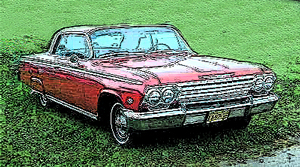
\includegraphics[height=30mm]{corps/chapitre10/img/voiture.jpg}
\end{floatingfigure}

Arrivée dans le bas de la ville de Québec vers 8 heures 30, Marceline gare la rutilante voiture sur la rue Saint-Joseph, presque au coin de la Couronne, à deux pas de l’Hôtel Saint-Roch. Elle s’empare du trousseau de clés, d’où elle retire celle de la malle arrière, et le remet sur le contact. Son plan est simple : ceux qui voleront l’auto éprouveront beaucoup de difficultés à mettre au jour le sépulcre d’Edmond. Ils prendront leur temps, soucieux de ne pas endommager une si belle automobile; il leur faudra bricoler et, au terme, quand le coffre finira par s’ouvrir, ils auront un cadavre sur les bras. Pendant ce temps-là, elle et Marie seront loin.

Avant de quitter, elle essuie d’un mouchoir tout ce qu’elle croit avoir pu toucher, elle abaisse les deux grandes fenêtres latérales de l’Impala et se met à marcher, Marie à sa suite, en direction du poste de taxis tout près de l’hôtel.

Assis dans sa Plymouth noire en train de lire l’Événement-Journal, un chauffeur les remarque et, du regard, interroge Marceline.

- Sur l’aut’ bord du pont de Québec, y a un restaurant avec plein de gars de truck. C’est là qu’on s’en va. Pis j’ai d’l’argent pour payer, ajoute-t-elle aussitôt en brandissant une partie de sa fortune.

Sans dire un mot, l’homme, habitué à d’aussi pathétiques cas de misère humaine, le quartier Saint-Roch étant ce qu’il est, accepte la course et les passagères s’installent sur la banquette arrière. Tout au long du trajet, la discrétion étant sa devise, il va se faire un devoir de ne pas les regarder par le rétroviseur.

- Ici ça fait-y, demande-t-il une fois le pont traversé. Le parking est plein de trucks et de vans.

- C’est b’en correct.

Yvette Carrier, serveuse responsable du comptoir dont les tabourets semblent plaire à certains clients, remarque, par une des grandes fenêtres latérales de l’établissement, un taxi de Québec duquel descend une adulte qui boite en se tenant les côtes d’une main et serrant celle d’une petite fille aussi amochée qu’elle de l’autre. Du coin de l’œil elle les regarde entrer et venir s’asseoir juste en avant d’elle. Comme elle a probablement tout vu ce qui était possible de voir, elle ne fait mine de rien et se tourne à nouveau vers la grande baie vitrée pour fumer sa cigarette.

- Ça va être quoi, les madames, demande-t-elle finalement, son carnet de factures à la main.

- On a faim, répond Marceline. On voudrait des œufs avec du bacon pis des toasts.

- Comment les œufs ?

- Virés de bord. Pis du café pour moi et du lait pour la p’tite.

Dix minutes après avoir été servies, ni l’une ni l’autre n’ont avalé quoi que ce soit. C’est à peine si la jeune femme a trempé ses lèvres dans le café.

- Sont pas bons, mes œufs ? questionne Yvette Carrier.

Marceline repousse son assiette en regardant Marie.

- C’est pas qui sont pas bons, c’est qu’ils passent pas.

- Ouin, ça pas d’l’air de filer pantoute, à matin ?

- Mettons que ç’a déjà été mieux.

- J’vois b’en ça !

- On s’en va dans ma famille à Rimouski, ment-elle.

Puis, après quelques secondes de silence.

- Il a pas mal dépassé les bornes cette nuit.

La serveuse tire sur sa cigarette d’un air entendu.

- Pauvre ‘tite madame, voir si ç’a du bon sens ! Pis c’te p’tite fille-là aussi. Y en a-t-y des chiens sales !

Le plan de Marceline semble se dérouler tel que prévu.

- Vous connaîtriez pas quelqu’un, des fois, ici dans votre restaurant, qui serait prêt à nous prendre jusqu’à Rimouski ?

Yvette Carrier la regarde un instant sans parler, puis lui fait un signe de patienter. Elle s’approche d’un quinquagénaire à casquette, un mal rasé en train d’avaler un déjeuner tardif, et amorce une brève discussion au cours de laquelle elle pointe à quelques reprises vers Marceline et Marie. Puis elle hoche de la tête et revient à son comptoir.

- Tony, là-bas, il va vous prendre. Il travaille pour Rimouski Transport et il fait la run Montréal – Gaspé. Il va vous laisser en passant. C’est un bon gars, même s’il est pas beau.

Comme son interlocutrice semble hésiter, elle ajoute :

- Vous avez pas besoin d’avoir peur.

Quinze minutes plus tard, Marie se retrouvait assise entre ledit Tony, grand sec à l’éternelle cigarette, et sa mère, une serviette de table mouillée tenue sur l’œil, dans la cabine d’un camion de livraison avec comme destination, le Bas-du-Fleuve. À quelques reprises, à voix à peine audible, le chauffeur va tenter d’amorcer une conversation, aussi bien avant qu’après la halte rituelle au Martinet de La Pocatière. Mais Marceline ne mordra pas et Marie sera muette comme une carpe dépressive. Cependant, à la hauteur du Bic, il ne pourra plus se contenir.

- Ce n’est pas de mes affaires, madame, mais Yvette m’a dit que la p’tite avait rien mangé et rien bu au comptoir. P’is tantôt au Martinet, elle a rien voulu prendre. Même pas un verre d’eau. Elle parle pas, elle bouge pas. C’est pas normal pour un enfant de son âge. À vot’ place, j’irais voir un docteur. Elle a un problème, c’est sûr.

- Ouin, c’est ce que je vas faire en arrivant à Rimouski.

Mais elle ne le fera pas. Car une fois descendues de l’énorme «Inter», Marie et elle marcheront trois pâtés de maisons jusqu’à une boutique de fleuriste de la rue Saint-Germain.

- Lise, fait-elle à une petite bonne femme toute ronde, rose et rieuse, j’ai besoin de toi.

Apercevant sa cousine aussi mal amochée, Lise Laplante, la propriétaire, s’exclame à grand renfort de gestes.

- Il vous a encore battues, le verrat ?

- Y a rien de neuf là-dedans, lui rétorque Marceline. Écoute, j’ai besoin de toi.

- Que c’est que je peux faire ?

Elle lui explique devoir absolument s’en aller chez elle, à Saint-Fabien. Elle en a à peine pour deux heures, mais elle ne peut amener Marie. Si Lise avait la gentillesse de la garder et d’essayer de lui faire avaler quelque chose, elle lui en serait reconnaissante.

- Elle a rien mangé depuis hier. A va pas bien. Et si en plus, tu pouvais me prêter ton char, ça m’aiderait pas mal.
Habituée aux extravagances de sa parente, Lise ne dit mot, ouvre un tiroir et lui tend un trousseau de clés.

- Le char est en arrière du magasin. Mais pourquoi que tu veux t’en aller à Saint-Fab, là, maintenant ?

- C’est une affaire de rien, mais j’peux pas t’en parler. Fais-moi confiance, y a rien de méchant.

\begin{floatingfigure}[l]{30mm}
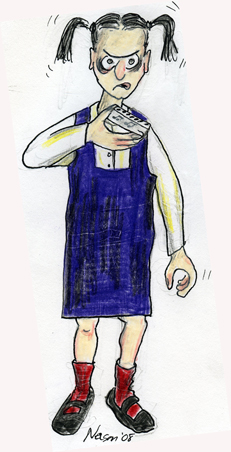
\includegraphics[height=50mm]{corps/chapitre10/img/personnage-marie-jeune.jpg}
\end{floatingfigure}

Une demi-heure plus tard, Marceline, la femme des Bezo, est chez elle en train de tout nettoyer «à grande eau». Il ne faut plus qu’il reste quoi que ce soit d’Edmond. Même pas l’air qu’il a respiré. Elle astique son prélart, lave verres et cendrier, brûle le linge à vaisselle, fait disparaître les traces de pneu qu’a laissées l’Impala en avant de la maison et les traces de sang laissées par la jambe, replace les bouteilles vides dans leur caisse, sans oublier le «40 onces» à moitié plein, place le tout sur la banquette de la voiture – elle les jettera dans les poubelles de sa cousine fleuriste - et fait le tour vingt fois. Ce faisant, son regard porte sur la grille d’air chaud et elle revoit sa gamine s’y amuser à l’observer et à lui parler au travers des orifices. Un doute vient l’habiter. Et si, hier soir, Marie avait été éveillée et avait vu toute la scène ? Ou une partie de la scène ? Elle ne dormait probablement pas, ce matin, quand elle lui a dit de sortir du lit; contrairement à son habitude, elle s’est levée immédiatement. Et si elle a vu quelque chose, elle est peut-être en état de choc, d’où la raison pourquoi elle ne mange pas, ne bois pas et ne parle pas. Et si elle débloque, qu’elle se met à raconter des choses ?

Inquiète, Marceline saute dans l’auto et revient à Rimouski le plus vite qu’elle le peut. Quand elle entre dans l’arrière-boutique de la fleuriste, elle constate que Marie est en train de grignoter une DairyMilk de Cadburry. L’ayant entendue arriver par l’arrière, la commerçante passe la tête sur le rebord du rideau qui agit comme porte entre la pièce et la boutique.

- Elle a d’l’air à filer mieux, explique la cousine Lise. Elle m’a dit qu’elle avait un peu faim. Fait que je lui ai donné d’la liqueur, un bon cream soda, et une bonne barre de chocolat. Hein ma chouette ?

Marie ne bronche pas.

- Ensuite, elle m’a conté qu’elle avait fait un beau voyage dans un camion avec un monsieur appelé Tony. C’est-tu vrai ça ?

Marceline hésite avant de répondre.

- Mettons qu’elle a une b’en grosse imagination. Surtout ces temps-citte !

- Ah ! Je sais c’est quoi ! J’en ai une du même âge à la maison. Ça en raconte, des histoires !

Ce soir-là, quand Lise les aura ramenées dans le 3e Ouest, toutes deux s’écraseront de fatigue. Marie aura peine à grimper jusqu’à sa chambre.

Le lendemain matin, pendant que Marceline est occupée à touiller sa soupane aux pommes et à la cassonade pour faire comme si de rien n’était, Marie descend, tout habillée, sa joue encore enflée. La mère, malgré ses pressentiments, tente de se faire le plus accueillante possible. Elle raconte être allée chercher les derniers fruits dans la cave pour préparer ce «bon gruau». Mais l’arôme du festin ne peut rien contre le visage dur, noir, mauvais de la fillette.

- J’en veux pas de ton gruau, je veux partir d’ici, Je veux plus être avec toi.

- Mais voyons, ma pitchounette.

- T’es méchante. Tu m’as pas défendue quand il m’a battue, tu l’as laissé faire quand il a détruit ma musique à bouche, ma belle musique à bouche, maudit ! Mais toi, par exemple, tu t’es défendue. Je t’ai vu le sortir. Pis après, tu m’as fait passer pour une menteuse chez matante Lise. J’veux p’us rester ici, j’veux m’en aller. T’es aussi méchante que lui ! P’is j’ai trop peur qu’il revienne !

Et l’enfant de déguerpir vers ses contrées imaginaires. Marceline ne la reverra que le soir et n’arrivera pas à lui parler. En fait, elle n’arrivera plus jamais à lui parler. Pire, personne, à l’exception de Rhéa Théberge, n’arrivera à le faire, et encore. Marie ne fera plus de devoirs, n’aidera plus en classe, ne touchera plus l’harmonium et écrira n’importe quoi sur ses feuilles d’examen de fin d’année.

Tant et si bien que le lundi 18 juin, début de la dernière semaine de classe, l’institutrice constate qu’elle va devoir recaler la petite, lui faire reprendre sa sixième année, elle qui en sait beaucoup plus que les grands de septième, tant la somme des points perdus depuis le début de mai est importante. Toutes ses tentatives d’en parler avec elle ont été inutiles, Marie s’étant refermée. Et malgré les pluies abondantes en cette fin de printemps, elle a préféré marcher les trois kilomètres matin et soir.

L’absurdité de la situation émeut Rhéa au point où sur la fin de l’après-midi, elle se pointe chez Marceline occupée à sarcler son jardin, un enclos cintré d’une ancienne clôture en pieux de cèdre désormais incapable d’arrêter les chevreuils. Marie n’étant visible nulle part, elle va droit au but. La petite est brillante, bourrée de talents, assoiffée d’apprendre. Pour tout dire, elle est de loin la meilleure élève qu’elle n’a jamais eue dans sa carrière. Mais il s’est passé quelque chose en début mai. Depuis, c’est la dégringolade. À pic !

- Saviez-vous, madame Rioux, que votre enfant joue de l’harmonium mieux que moi ?

Aucune réponse. L’enseignante constate que son interlocutrice semble davantage intéressée aux manœuvres d’une libellule. Mais elle poursuit.

- Saviez-vous qu’elle sait lire et écrire de la musique, clé de sol, clé de fa ? Qu’elle a lu, cette année, un livre par semaine, incluant tous les Marcel Pagnol que j’ai pu trouver ? À onze ans ? Qu’elle faisait faire leurs devoirs aux plus jeunes ?

- Ouin, elle m’en a parlé.

Marceline a de la difficulté à ne pas rougir devant un si grossier mensonge. Elle se ressaisit et ne donne pas à Rhéa Théberge le temps de poser une nouvelle question.

- Écoutez, mam’zelle Théberge, je sais que ma fille est pas pire, mais je vois pas où c’est que vous voulez en venir.

- À ceci !

L’enseignante ouvre brusquement sa mallette en cuir brun. Elle en extirpe quelques feuilles qui, explique-t-elle, démontrent que Marie n’a pas répondu aux questions des examens. Et, avec le passif accumulé depuis le début mai, elle ne peut être promue en septième, ce qui constitue une aberration majeure. À un point tel, qu’on ne peut se contenter de ne rien faire, ce qui suppose qu’il faut absolument la changer de milieu. Lui donner une chance d’assumer son potentiel. De toute façon, il faut se faire à l’idée qu’elle est à la veille de «changer d’air». Dès le secondaire, elle devra effectivement passer ses semaines en bas, au village, chez des parents, chez des amis ou dans une pension. Il lui sera devenu impossible de voyager matin et soir. Aussi bien devancer d’un an, non ?

Marceline commence à être agacée.

- Pourquoi vous me dites tout ça, là ?

- Parce que je veux vous aider à lui trouver une place quelque part en ville pour qu’elle fasse sa septième année. J’ai pas le droit, mais je suis prête à arranger ses notes pour qu’elle monte quand même.

- Où en ville ?

- À Rimouski, à Québec, à Montréal. Quelque part où elle sera prise en charge et où elle pourra faire des études à sa mesure. Madame, votre fille est brillante et, ici, dans les rangs de Saint-Fabien, elle est bloquée, fermée, en état de régression.

Rhéa Théberge lorgne le jardin comme si elle voulait inventorier les espèces qui y poussent.

- Et, si je l’ai bien comprise, elle a une peur bleue de son père …

- Son père, ça fait un siècle qu’on l’a pas vu, coupe la femme des Bezo.

- Elle doit partir, madame, c’est pour son bien.

- Écoutez donc, vous ! J’vous trouve b’en effrontée.

- Madame Rioux, j’aime beaucoup votre fille. Elle mérite qu’on s’en occupe, qu’on lui dégote une place quelque part.

Marceline tente de pénétrer l’intérieur des yeux de Rhéa.

- Elle va vraiment doubler son année ?

- Oui, ses notes sont terribles.

- Mon Dieu seigneur !

- Dites-moi juste que vous allez y penser.

Pour y penser, elle va y penser ! Et sans perdre de temps.

Deux jours plus tard, Marceline va débarquer chez sa cousine fleuriste à Rimouski et quand elle en repartira en fin de soirée, le sort de Marie aura été tracé. La fillette, dont l’imagination est très fertile au point qu’il faut s’en méfier, sera placée en pension chez «matante Lise» et le plus tôt sera le mieux. Durant l’été, elle rendra service dans la boutique. Par exemple, elle fera le ménage, elle apprendra à faire des bouquets, à livrer de petites commandes et même à recevoir les clients. Sans compter qu’elle pourra devenir amie avec Colette, la fille unique de Lise. Et, en septembre, elle ira faire sa septième année à l’école Saint-Pie-X, à deux pas de la maison des Laplante, ce qui ne l’empêchera pas de continuer à donner un coup de main au commerce de la rue Saint-Germain pour rembourser sa pitance. Ensuite, on verra !

Ce qui fut fait. En un an, il se passa quatre choses importantes dans la vie de Marie Rioux, plus jamais Bezo. Loin de sa mère, loin du 3e Ouest, repliée sur elle-même, elle se transforma, dès septembre, en première de classe un peu chipie et ne laissa jamais personne, même les jumelles Thibault, les filles du docteur, lui ravir sa place. Puis, en octobre, elle découvrit un violoncelle enfermé dans le placard du salon, un instrument dont se targuait de jouer, à l’occasion, ce bon diable de Lucien Laplante, le mari tout rondelet, jovial, inoffensif et soumis de Lise. Comme si cela allait de soi, elle se l’appropria et entreprit d’en tirer des sons avec l’aide complice de son propriétaire, une aide enjouée qu’elle toléra néanmoins avec distance et prudence, ainsi qu’avec les conseils occasionnels de Rhéa Théberge qui venait la visiter de temps à autre. Ensuite, en décembre, la fillette refusa énergiquement d’aller passer le congé des fêtes chez Marceline. Elle tint tête à tout le monde et vécut son premier Noël, pour peu que ses souvenirs soient fiables, sans grincements, sans pleurs, sans alcool et sans violence. Enfin, en mars, le conflit avec sa cousine Colette devint insoutenable. Le caractère de l’une étant mauvais, la jalousie de l’autre atteignant des sommets, les deux jeunes filles cessèrent à tout jamais de se parler. Tant et si bien qu’à la fin de l’année scolaire, il fut convenu de retourner Marie chez sa mère.

********************************

Il ne reste plus qu’un long paragraphe, presque toute une page calligraphiée, avant que la lettre de Marceline ne soit terminée. Ému, Timothée poursuit sa lecture, déchiffrant, sans humeur, le texte constellé de fautes et de tournures laborieuses. Tellement qu’il lui arrive de devoir reprendre des passages jusqu’à trois fois avant d’en saisir le sens.

- «Mais il y avait un homme qui vivait avec moi, récite-t-il au bénéfice de Romain qui fixe les motifs du tapis. Quand tu as vu ça, tu ne l’as pas accepté du tout. Tu n’as pas voulu rester avec moi une minute de plus. Tu avais très peur et tu m’en voulais encore. Autant que l’année précédente. Tu as crié. Tu as tout fait pour t’en aller. Ce qui fait que j’ai fini par te placer chez ma sœur Denise à Québec. En attendant, tu es allée coucher chez Mlle Théberge. Et comme je craignais que tu leur bavasses tout, je leur ai dit qu’au sujet de ton père, tu racontais des histoires tirées de ton imagination et qu’il ne fallait pas qu’elles te croient. Ça m’a fait beaucoup de peine, je t’aimais tellement. À partir de là, tu as continué de t’enfermer encore plus creux dans ton monde de musique où tu étais à l’abri de tous ceux qui pouvaient te faire mal.» Ouin, Maman et sa musique …

- Continue …

- « Quand ton père à brisé ta musique à bouche, c’était ton monde qu’il massacrait. Sur le coup, je ne l’ai pas compris et tu m’as haïe parce que je n’avais rien fait pour l’empêcher. Pourtant, tant que tu as été avec moi, j’ai toujours essayé de te protéger, mais il faut croire que je n’en ai pas été capable comme il aurait fallu, comme tu l’aurais voulu. Après, j’ai essayé de te parler, mais tu n’as jamais voulu. Ce qui fait que je me suis contentée d’avoir de tes nouvelles par Denise que j’ai appelée toutes les semaines. C’est comme ça que j’ai su que tu étais toujours la première de ta classe et que tu étais entrée au conservatoire où tu étais la meilleure. Mais ça, ce n’est plus mon histoire. Elle est finie mon histoire. J’ai déclaré que ton père avait disparu et la police ne l’a jamais retrouvé.»

Romain se désenrhume.

- Sacrament !

- Attends ! Ce n’est pas terminé. «Bonne chance, ma petite Marie, je t’ai toujours beaucoup aimée et je t’aimerai toujours. De ta maman Marceline Belzile qui te demande pardon pour ne pas avoir été capable. C’est à mon amie, madame Rose Joncas, que je vais donner cette lettre pour qu’elle te la donne.»
\chapitre{La théorie du docteur Robie,le lundi 25 juillet 2033}{Si Timothée s’en donnait la peine,}{ il est probable qu’au bout d’une demi-heure de fouilles dans le prodigieux foutoir de Robespierre Alcide, il pourrait repérer dans les empilades de livres, de savantissimes ouvrages signés John Stuart Mill, Pierre Janet, Henri Wallon, Jean Piaget, Daniel Lagache, Juliette Favez-Boutonnier et, noblesse oblige, Sigmund Freud. Et s’il les ouvrait, il est quasiment assuré qu’il les trouverait maculés de soulignements et d’annotations en marge. C’est que le récréologue paradoxalement le plus qualifié et le plus désœuvré de Rimouski tâtait sérieusement de la psycho. Un jour, il avait expliqué à son presque voisin de bureau que s’il avait la chance de revenir au monde, il se ferait «psychologue clinicien», une sorte de magicien capable de faire le bien, de guérir la souffrance, d’améliorer le sort des gens, cela sans jamais faire l’apprenti sorcier, sans jamais prescrire de Pétépano et sans jamais fournir de pilules du bonheur. }

Il se ferait un devoir de poser des diagnostics basés sur des constats réels, vérifiables, quantifiables. Il accorderait beaucoup d’importance aux faits ayant pu marquer la vie de l’être en détresse ayant fait appel à ses services, une personne qu’il considérerait comme étant un cas unique méritant d’être traité comme tel. Mais voilà, il tenait le temps dans un capharnaüm contre-productif et surchargé, payé à ne rien faire en raison d’un règlement dont l’esprit n’avait pu être inclus dans la formulation.

La veille, après la lecture de la lettre de Marceline, cette femme dont ils ignoraient à peu près tout jusque-là, Timothée et Romain s’étaient retrouvés un peu assommés. Ils étaient loin d’imaginer que Marie avait été une enfant malmenée à ce point et ils n’avaient jamais entendu parler d’Edmond Rioux en ces termes. Depuis toujours, la thèse véhiculée était que cet «écoeurant» avait fui le domicile conjugal sans laisser d’adresse et n’avait plus jamais donné de nouvelles. C’est ce qui avait forcé Marceline à se trouver un emploi dans un magasin de coupons et Marie, à aller demeurer chez sa tante Denise. Si cette lettre n’était pas un tissu de fabulations, si elle n’était pas la divagation d’une démente perdue dans son alcoolisme, elle remettait beaucoup en question. Et la seule personne apte à faire la part des choses était la destinataire elle-même.

Très hésitants devant la marche à suivre, tous deux avaient alors convenu qu’il fallait demander de l’aide. Ils ignoraient comment allait réagir Marie s’ils l’en informaient. Ils appréhendaient que le rappel d’une histoire aussi terrible rende la vieille dame encore plus malade qu’elle ne l’était. En revanche, ils estimaient possible que le fait de ne pas connaître tous les «tenants et aboutissants» du drame et de pouvoir lire la version de sa mère lui fasse le plus grand bien. Sauf que tête de pioche comme elle l’était, il se pouvait aussi qu’elle réagisse très mal et qu’elle leur fasse regretter l’initiative. Mais à qui pouvaient-ils demander de l’aide ? Les trois psychologues à l’emploi du Centre étaient des carriéristes qu’on ne pouvait décidément pas mettre dans la confidence. Quant à aller consulter un privé, les tarifs horaires exigés avaient de quoi décourager les gens honnêtes. Le fils avait alors eu l’idée de quérir l’avis de Robespierre, homme de précieux conseils, notamment pour les questions psychologiques, et le père avait approuvé. Cela impliquait cependant qu’on lui dise la vérité, qu’on lui révèle l’existence de la Maririou et de Romain. Pouvait-on faire confiance à cet étrange personnage ?

- Sans l’ombre d’un doute, avait répondu Timothée.

Et ce matin, quand il lui avait dévoilé le pot aux roses, la réaction n’avait témoigné d’aucunes surprises.

- Je te remercie pour cette preuve d’amitié. Mais figure-toi que je m’en doutais un peu. On ne me demande pas deux pilules du bonheur pour aller remonter la rivière Rimouski en canot.

Timothée lui avait alors présenté le manuscrit, lui recommandant de le lire attentivement afin d’être en mesure de bien le conseiller quant à la marche à suivre.

- Mon père et moi on ne sait vraiment pas quoi faire.

\begin{floatingfigure}[l]{40mm}
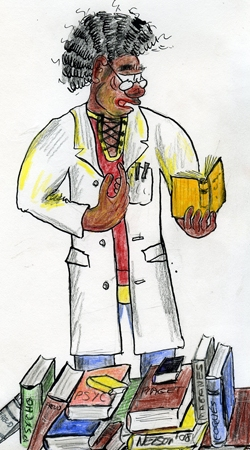
\includegraphics[height=60mm]{corps/chapitre11/img/personnage-robespierre-psy.jpg}
\end{floatingfigure}

Tandis que Robespierre, lunettes rondes sur le bout du nez et sarrau de clinicien par-dessus son chandail de football, est profondément plongé dans l’intimité de Marceline, cela depuis un gros dix minutes, Timothée, les yeux cernés comme il ne les a jamais eus, se sert de la fonction téléphonique du quanticordi pour essayer de se procurer un nouveau DPP. En même temps, les enceintes diffusent du Dylan :

    Combien de fois un homme doit-il regarder en l’air
    Avant de voir le ciel ?
    Oui, et combien d’oreilles doit avoir un seul homme
    Avant de pouvoir entendre pleurer les gens ?
    Oui, et combien faut-il de morts pour qu’il comprenne
    Que beaucoup trop de gens sont morts ?
    La réponse, mon ami, est soufflée dans le vent,
    La réponse est soufflée dans le vent.

Timothée lève les yeux.

- Dis, Robespierre, tu baisses ta musique, un peu ?

- Ça se peut-y que tu ne l’ait pas rechargé ? fait la voix du technicien. J’demande ça d’même …

- Non. Ç’a rien à voir, je l’ai toujours bien rechargée, ma fichue boucle d’oreille.

- T’es bien certain ?

- Oui !

- T’es certain que t’as pas pris ta douche avec ?

- J’suis pas si cave que ça ! Dites donc, vous me prenez pour qui ?

- Ouh ! Y est pointu à matin, le Motté !

- Oui, vous avez raison, je suis un peu fatigué.

- Grosse fin de semaine ?

- Ouin, c’est ça.

- OK. Rappelle-moi tes coordonnées.

- Timothée Tardif, CS-1, 5e Nord.

- OK. T’as rien qu’à passer avec ton vieux DPP, j’vas t’le changer.

- Parfait, à tout à l’heure !

Le premier message de sa boîte vocale est de Claude Sey, ce jeune agent de communication à l’emploi de Philippe «Flipper» Dauphin qui demande qu’on le rappelle le plus tôt possible en mode confidentiel. Ce que Timothée s’empresse de faire. C’est ainsi qu’il apprend que Louis-Marc Richard, son abject voisin de la rue Crouet, a reçu la visite d’un gorille du Flipper et qu’au terme, un rapport de six pages a été entré dans le système. Pire, une demande officielle d’enquête vient d’être acheminée au service de la sécurité. Ce serait en rapport avec le Dr Gagnon.

- À bon entendeur !

- Merci monsieur Sey.

Robespierre le fixe de ses grands yeux interrogateurs, ceux qui intimident habituellement Timothée.

- C’est quoi déjà le cliché habituel, Robespierre ? Ah oui : «l’étau se resserre».

- Qu’est-ce que tu veux dire ?

- Je viens d’apprendre que j’ai la Sécu aux fesses.

- T’as vraiment pas une vie singulière, toi. Je suis très heureux de te connaître.

- Merci.

- Mais là, j’ai un gros problème. Il faut que je relise bien attentivement et c’est pas facile. Y a tellement de fautes que c’est parfois illisible. Ensuite, va falloir que je réfléchisse. Va peut-être falloir que je bouquine pour bien comprendre. Donne-moi une couple d’heures. C’est trop délicat, je veux pas te donner n’importe quel conseil.

- Merci.

Le colosse lui fait signe de déguerpir.

Privé de Saguewanish, le CS-1 démarre sa tournée routinière du matin, à pied, une démarche surréaliste compte tenu de tout ce qui lui pend au bout du nez. Comment peut-on se promener à ne rien foutre dans un couloir qui empeste le vieux alors que tout foire autour de soi ? «Comment peut-on danser quand notre Terre tourne ? Comment peut-on dormir quand nos lits sont en feu ?» Comment peut-on respirer quand nos aînés sont nourris avec ce margouillis de Nutrisuz ? Comment peut-on ne pas fuir, là maintenant, pour l’île d’Anticosti ? Pourtant, le salon communautaire semble normal; le 500 y bat son plein avec ses accrocs habituels, les Marven, Beaulieu, Jean et compagnie. Mais assis dans le fond, à quelques mètres de Mme Bellow, le couple Martel est en conversation. Nouveau ça ! Y caresse-t-on des projets ? S’y remémore-t-on le passé ? Va-t-on demander une autre nuit d’intimité ? Un peu plus loin, devant l’écran du terminal quanticordi CLTD, Mme Labbé s’emmerde à regarder de vieux clips pas de son. Est-elle brouillée d’avec sa copine Thériault qui a d’autres chattes à fouetter ? Ici, la dame à moitié chauve essaie de ne pas somnoler devant la télé dont on a coupé le son, là Jean Saint-Gelais semble être à l’affut d’un mauvais coup à faire.

Comme il quitte pour cheminer jusqu’à la première salle 2P, Marie-Odile descend de l’ascenseur, en équilibre sur sa bécane. Apercevant le chef de section, elle le hèle à la manière d’un sergent-major à moustache et, l’accélérateur au maximum, fonce sur lui. Son visage aux antipodes de celui qui se béatifiait dans les langueurs lascives, charnelles et méritées du week-end, est devenu celui d’un inspecteur cocu qu’on a rétrogradé à la circulation et qui entend le faire payer très cher aux automobilistes, ces salopards. Le fils de la Maririou sait maintenant à quoi s’attendre. Froidement, sans dégainer, de toute façon les agents de la Sécu ne sont pas armés, elle lui ordonne non pas de s’appuyer les mains au mur et d’écarter les jambes, mais de la recevoir chez lui, dans son officine, à porte fermée, officiellement !

À peine assise, le verbe venimeux, l’œil pugnace et la griffe sortie, elle se dit d’abord «excessivement déçue». La direction générale lui a demandé, ce matin, d’enquêter sur le CS-1 Timothée Tardif. Mercredi dernier, dans la matinée, sur le temps du CRG, il aurait été vu en consultation précipitée à la clinique privée du docteur Étienne Gagnon, soi-disant pour une urgence. Tous deux seraient partis sur les chapeaux de roue, malgré les patients qui attendaient leur tour. Or il a été établi que le docteur Gagnon n’est pas passé au Centre ce jour-là. Question : si l’urgence ne concernait pas des bénéficiaires du Centre et si, lui, Timothée, semble ne pas avoir besoin de soins d’urgence, si c’est vrai ce qu’il dit à «ceux ou celles qu’il amène manger au Vieux Cormier» à savoir qu’il n’a pas de vie en dehors du Centre et de son domicile à Nazareth, à qui étaient destinés les soins d’urgence ? Et que penser de cette déclaration d’un certain Louis-Marc Richard, déclaration consignée par Philippe Dauphin devant témoin, selon laquelle il se passerait des «choses étranges» dans la résidence dudit Timothée Tardif ?

Si on fusionne ces deux rapports, n’est-on pas en droit de se poser de sérieuses questions ? Par exemple, qu’il pourrait y avoir des embrouilles probablement répréhensibles dont Timothée ne lui a pas parlé à elle qui s’était abandonnée à lui. «Après tout ce qui s’est passé», il aurait pu, au moins, avoir la décence de tout lui dire ! Mais pour cela, il aurait fallu qu’il lui fasse confiance. Qu’il s’intéresse à autre chose qu’à la bamboula. Bref, elle est blessée, elle se sent flouée, elle se croit trahie. Et elle, la femme flic, elle veut savoir ce qu’il en est. Maintenant ! Avant qu’elle n’aille interroger le docteur Gagnon et le dénommé Richard.

Un jour, Timothée avait peut-être dix ans, l’auto familiale s’était fait arrêter pour excès de vitesse. Furieux, le patrouilleur avait remis sa contravention à un Romain très silencieux, puis s’en était retourné dans sa voiture banalisée en faisant claquer la portière.

- Pourquoi il n’est pas content le monsieur ? Parce que quand il m’a intercepté la semaine dernière, il m’a donné une chance. Mais aujourd’hui, il voit bien que je n’ai rien compris. Il est déçu, il me laisse tomber et il me colle un sacrament de gros ticket !

Cette histoire lui était restée dans la tête et il regarde maintenant Marie-Odile avec la sensation que les carottes sont cuites. Un instant, il songe aux pilules du bonheur. En serait-on rendu là ? Comment serait-ce possible qu’on ne le soit pas, qu’il n’ait pas à poser un geste définitif en remettant les cachets à ses parents ?

Pour un ex-puceau de fraîche date, sa réponse est habile.

- Ça rien à voir avec toi en tant que femme, mais avec toi en tant que police. Je ne t’ai rien dit parce que si je le fais, tu vas devoir faire un rapport, ce qui déclenchera mon congédiement et bien pire encore. J’ai pas passé la fin de semaine avec une flic, mais avec une femme. Et j’ai aimé ça.

Elle encaisse le coup.

- Mais c’est quoi qui faut pas que je sache qui est si important ?

- J’peux pas te le dire. Notre conversation est probablement en train d’être numérisée par la microcam intégrée dans le premier bouton de ta chemise, ce gadget dont tu m’as parlé vendredi midi à la pizzeria, et c’est relayé au 2e étage comme pièce incriminante devant être versée à mon dossier. Désolé, ajoute-t-il en lui tendant les poignets, écris dans ton rapport que j’ai refusé de collaborer.

- Pour l’instant, personne ne m’a encore demandé d’enregistrer quoi que ce soit. Mais juste au cas …
Elle extirpe d’une de ses poches de bermuda un zinzin noir de la taille d’un cube de sucre. Du pouce, elle l’écrase : clic !

- Les ondes sont maintenant brouillées; c’est plus possible de rien numériser.

Il lui scrute longuement les yeux et ce qu’il y discerne l’incite à plonger, allez savoir pourquoi. Alors, il raconte tout. La coke, le feu, Alessandro, la loi du Gros Turcotte, le sous-sol, le voisin chiant, la maladie de sa mère, le docteur Gagnon, les conditions épouvantables de paiement et son désarroi. Il omet cependant de mentionner cette lettre qu’il a remise tout à l’heure à Robespierre. Pourquoi l’aurait-il fait ? N’y parle-t-on pas de meurtre au premier degré avec circonstances atténuantes discutables ? L’heure que nécessitera cette confession sera ponctuée de coups frappés à sa porte et de sonneries de téléphone : Ronnie Ross, de 8 à 4 cette semaine, qui veut lui parler du père Jean, Solange Gadoury qui insiste pour faire valoir un point de vue, l’infirmière Béatrice Martin qui offre son aide s’il le juge nécessaire et Shimoune Saint-Pierre qui affirme avoir de l’info intéressante pour lui.

- Ton histoire a tellement pas de bons sens qu’elle doit être vraie !

- Je t’ai tout raconté. Et maintenant ?

Elle se lève et se place les mains sur sa Saguewanish.

- Et maintenant, je vais réfléchir.

Comme elle ouvre la porte, Robespierre apparaît.

- Tiens, bonjour Marie-Odile, lui serine-t-il les lèvres tout en appétit.

Elle le salue sèchement de la tête, hésite un instant et file vers l’ascenseur. Elle a oublié de désembrouiller les ondes.

- Tu peux parler librement, le nécessaire a été fait pour que ça soit impossible de numériser les conversations.

- Méchantes belles relations !

- Et alors ?

- B’en ça m’en dit beaucoup sur toi et sur ta mère.

Et voilà le Robespierre, docteur Robespierre, en frais de décortiquer la longue lettre de Marceline et d’interpréter ce qu’il y a découvert comme états d’âme, nature humaine, traits de personnalité, séquelles psychologiques, voire dommages permanents, le tout à l’aide de ses maîtres à penser, certains étant cités dans le texte. Ainsi, Marceline n’est pas la dépendante affective typique qui a besoin d’être prise en charge, dominée, par un homme. Elle n’est qu’une malchanceuse qui s’amourache d’un beau voyou, Edmond Rioux, qui arrive à la battre simplement parce qu’il est beaucoup plus costaud qu’elle. Sinon, c’est probablement elle qui le rouerait de coups. Le gars est une brute qui idéalise la violence laquelle est confondue avec expression de la virilité et sens de la réplique. Ce que Marceline ne conteste pas, du reste. Les bagarres de son époux dans les bars, sa valorisation masculine, son obligation de la violer pour commettre l’acte sexuel, sa facilité à frapper sa fillette, sans oublier sa misogynie évidente, sont autant de pistes pour supposer que ce personnage est un homosexuel refoulé.

- Il y a soixante ans, personne ne quittait son placard. On se contentait de prouver le contraire en battant tout le monde. C’est simple : en 1962 «tapette» égalait «fif qu’on roue de coups» et «vrai gars» égalait «brute virile hétéro que l’on craint». Ce que je dis est tellement documenté que c’est quasiment devenu un poncif.

Quant à Marie, ses réactions sont toutes conformes au manuel, soutient le psychologue autoproclamé. Élevée sans tendresse, elle grandit dans la crainte d’un homme immense, bruyant, imprévisible, alcoolique, violent et dangereux, bref, un ogre épouvantable. Elle s’habitue à une mère disgracieuse, une femme violée, violentée, incapable de se faire respecter et de protéger son enfant, une malheureuse qui tente d’oublier en jardinant, en buvant et en s’acoquinant au village pour au moins avoir quelqu’un à qui parler, autrement dit, une personne en grand désarroi, en grande souffrance. La petite fille est amenée à la musique, à la culture et au savoir, elle est initiée à la tendresse, à la générosité, au respect et à la valorisation, par son institutrice, la seule à voir en elle autre chose qu’une misérable Bezo sur qui on peut taper sans conséquence.

- En gros, il y a une sorte d’image manichéenne qui s’est formée dans son esprit de survivante : d’un côté le monde des méchants, de l’autre celui des gentils. Dans le premier, il n’y a pas de musique, dans l’autre, il y en a. J’ignore ce qu’il en est dans sa vie, à ta mère, je n’ai jamais eu le plaisir de la rencontrer, mais, à la lecture du document, je ne serais pas étonné d’apprendre qu’elle ait passé sa vie à trembler devant les forts en gueule, les gros bras, les meneurs de claques, les clous de soirées ou encore les hommes qui semblent s’intéresser à elle sans qu’elle ne l’ait décidé. Je suppose que ton père, pour qu’il soit ton père et qu’elle tolère qu’il continue de l’être, a dû être tout le contraire, toute sa vie, c’est-à-dire un homme doux, tolérant, facile à vivre, de bonnes compagnies, qui lui a toujours passé ses caprices et ses volontés. Ai-je tort ?

- T’es dedans à 100 %.

- J’en déduis qu’elle t’a élevé pour que tu ne sois pas un mâle alpha, pour que tu sois vraiment doux, presque silencieux, sobre, fidèle, solitaire comme elle et dévoué à sa personne, voire capable d’en prendre soin sur ses vieux jours. Mais ça, je n’ai pas à te demander ton avis, je sais que tu as ce genre de comportement.

Un comportement n’ayant que fort peu à voir avec celui du vrai Timothée de Milet, l’homme de la Lyre à onze cordes.
Un frappement précède l’ouverture de la porte. Ronnie Ross se fait insistant.

- Excuse, Motté, siffle-t-il en ignorant Robespierre, ce qui est la chose habituelle à faire, mais faut que j’te dise au sujet du pére Jean. Ils l’ont descendu au sous-sol.

- Qui ça ? La Sécu ?

- Ouin. Tropecolo le Chinois et Tremblay la Bitch. Paraîtrait que c’est lui qui a bousillé ta saguigui.

Timothée réfléchit un instant.

- C’est quoi le topo avec les bénévoles cette semaine ? Depuis vendredi, le père Jean passait ses fins de journée avec monsieur Lafrance en 3P-L. Si c’est comme la semaine dernière, on a un problème.

- Ouin, le bonhomme ‘i est rendu écœurant; faut ‘i changer ses couches aux heures. J’en n’ai jamais vu des puantes de même ! On n’a rien qu’à le transférer en palliatif, la cérémonie va avoir lieu dans une semaine. D’ici c’temps-là, on va pouvoir s’arranger.

- J’vais y penser. En attendant, peux-tu vérifier pour les bénévoles ?

- J’vas aller voir.

Le préposé parti, Robespierre s’assure que la porte est bien refermée et il poursuit ses explications.

- Comme résultat de son enfance, ta mère a probablement peur de s’impliquer avec les gens, de travailler en équipe. Elle va rechercher la solitude, fuir les mondanités, la société. Par instinct, par méfiance, par réflexe de survie, elle refusera de s’ouvrir, d’échanger de façon intime. Elle craindra qu’on lui fasse mal. Elle voudra se protéger. Et si ça se peut ce que je viens de dire, sa vie sexuelle sera misérable. Pour elle, faire l’amour équivaudra à se laisser aller avec un homme désireux de la posséder, la soumettre, la violenter. Dès lors, l’image impitoyable, brutale, douloureuse du père se substituera. Mais ça, il est plus que probable que tu ne le saches pas; par contre, ton père, lui …
Timothée hoche horizontalement de la tête. Va pour la vie sexuelle, mais pour s’impliquer avec les gens, c’est une autre histoire.

- Toute sa vie, elle a été musicienne, elle a joué dans des orchestres symphoniques importants, ici, elle s’est occupée de l’École de musique…

- Ce n’est pas parce que tu joues dans un orchestre symphonique que tu es attentif aux autres; tu es peut-être claquemuré dans ton monde à toi en train de lire des partitions, parce que la musique est la seule thérapie qui t’ai gardé en vie. Mais écoute, Timothée, mon échafaudage n’est que de la théorie; je ne connais pas ta mère du tout. Et puis je suis loin d’être un psy; je ne suis que Robespierre Alcide, arrière-petit-fils de l’inventeur du Pétépano. Quant à ta question de ce matin sur le document, à mon avis, il faut le donner à ta mère en lui disant toute la vérité. Ça lui revient. Béatrice Martin te l’a remis, toi et ton père vous l’avez lu parce que vous n’aviez aucune idée de quoi il s’agissait. Maintenant que vous le savez, vous croyez vraiment que ça peut lui faire du bien de le lire, pour peu que son contenu soit vrai, et, surtout, vous n’en dites pas plus, vous ne lui laissez pas sentir que vous aimeriez en parler.
De nouveaux coups se font entendre. C’est encore Ross, mais cette fois il se bouscule littéralement avec la mère Gadoury et il finit quand même par entrer.

- Méchant problème, Motté. Ils nous ont pas trouvé de bénévoles cette semaine. Va falloir se débrouiller.

- Y est pas question que vous transfériez Lafrance au mouroir, griche Mme Gadoury, ses petits doigts boudinés faisant comme s’ils étaient griffus.

Le CS-1 enlève ses verres pour se frotter les yeux et il fixe Robespierre en haussant les épaules. Le colosse se lève aussitôt et disparaît dans le large couloir.

- Toé, le vieux hibou, tu te mêles pas de nos affaires, t’as-tu compris ?

- Ronnie, câlisse ! Mme Gadoury veut juste … Ah bof !

Un instant, plus personne ne parle.

- Bon. On va se démerder comme le mois dernier; on va mobiliser nos bénéficiaires des salles 2P. Tant pis pour les humeurs !

Sentant qu’il pourrait lui en cuire - n’est-elle pas elle-même hébergée en salle 2P ? – Solange Gadoury disparaît dans le sillage de Robespierre Alcide.

Arrivés au poste de garde, Timothée, Ronnie et Steve Grenier, l’autre préposé assigné cette semaine au 8 à 4, ont tôt fait, liste en main, d’affecter leur clientèle la moins «poquée» selon les besoins du premier et du deuxième quart de travail. Tout le monde y passe, incluant Mmes Gadoury et Bellow. La première pour faire une fleur à Ronnie, la seconde parce que le CS-1 entend la ménager à sa façon.

- Madame Bellow, suivez-moi, lui dit-il, une demi-heure plus tard quand tout un chacun, dans un concert d’indignations, a reçu son affectation.

Docile, la vieille dame lui emboîte le pas.

- Je vous vois mal passer la moppe, donner le manger mou aux impotents ou changer des couches en salle palliative.

- Mais si, je peux faire ma part.

- Je le sais, mais il y a mieux à faire. Vous connaissez monsieur Alcide ? lui demande-t-il en cognant à la porte de Robespierre.

- C’est pas barré, entend-on.

- Mon ami monsieur Alcide, voici madame Bellow, détentrice d’une maîtrise en bibliothéconomie de l’Université de Montréal.

Le sportif réglementé reçoit cette preuve d’amitié comme un pavé d’asphalte tombé dans sa soupe.

- Avez-vous déjà vu ça, madame Bellow, un bordel de livres comme ça ?

- Non, monsieur Tardif.

Robespierre n’ose parler.

- Écoute, madame Bellow est bénévole pour te conseiller dans ton classement. Entre diplômés universitaires et rats de bibliothèque, vous allez sûrement vous entendre.

- C’est très gentil, mais … je me comprends très bien dans mon bordel !

- Regarde, c’est rien de vraiment compliqué. Il s’agit seulement de t’assurer que Ronnie ou Steve ne l’attraperont pas pour l’envoyer changer les couches de monsieur Lafrance ou laver les toilettes dans les 3P. Défends-la sur ton honneur de grand chevalier noir. Et, qui sait, peut-être qu’en retour, elle va vraiment t’aider dans ton foutoir.

Et là-dessus, le CS-1 file vers l’ascenseur. S’il a de la chance, il pourra descendre au soutien technique, situé au rez-de-chaussée sud, où on lui remettra une nouvelle boucle d’oreille. Mais il n’en a pas; c’est comme si la fatalité s’acharnait à le priver de moyens de communication et de transport. Cette fois, c’est Marie-Odile qui l’attend au poste de garde. Elle a quelques papelards électroniques à lui faire signer relativement au sabotage de sa Saguewanish. Au moment où elle lui tend le stylet, Steve Grenier, une des pires langues du CRG-BSL passe et les gratifie d’un sourire narquois.

- T’as d’la belle visite, le Motté ?

La femme flic lui lance un regard tellement mauvais que le grossier personnage entreprend de se fondre dans le revêtement mural. Replaçant le mini ordi tactile dans sa petite housse en cuir, elle lui raconte que durant la fin de semaine, son collègue David Gagnon- Tropecolo, alias Tropecolo le Chinois pour cause d’épousailles avec une dame de Shanghai, a ouvert une enquête et s’est promené sérieusement dans les locaux du 5e Nord. Il n’a pas mis trop de temps à repérer quelques maillons faibles dans la défense du suspect et à les faire craquer un à un. Trois témoins ont signé leur déposition inculpant Jean de méfait sur des biens de la couronne. Redoutable le Tropecolo !

- Ce matin, en arrivant, il est parti se chercher une autorisation chez Carl Michaud. Ça nous a permis, lui et moi, d’aller ramasser le bonhomme ici à côté dans le salon et de le descendre en bas dans un «local de réflexion».

- Vous allez faire quoi avec ?

- Rien. Il va croupir là au moins jusqu’à l’hiver. La direction générale a décidé de pas porter plainte à la police.

- Ça va se régler à l’interne.

- C’est ça.

Est-ce dû à la gêne qui s’ensuit ? C’est comme si, de cette crevasse de silence qui s’est excavée entre eux, on préférait subir le dégagement des gaz volcaniques, le grondement des entrailles de la Terre et le surgissement des démons de l’enfer. C’est Marie-Odile qui casse néanmoins la glace.

- J’achève ma réflexion et j’aimerais t’en faire part.

- Bien sûr. Euh … Tropecolo est-il au courant pour mon histoire avec le docteur Gagnon ?

- Non. C’est mon dossier.

La bonne nouvelle, elle est seule sur l’affaire. La mauvaise ? Elle est seule sur l’affaire !

- Tu pourrais passer chez moi, ce soir vers 19 heures, si ça te convient.

- Ça marche. Mets une bouteille au frais, ajoute-t-il en le regrettant instantanément.

Pourquoi a-t-il dit cela ? Qu’est-ce qu’il lui a pris ! «Quel idiot tu peux être», le chicanerait sûrement Quetzalcoatl. Marie-Odile ne semble pas l’avoir apprécié non plus, car elle vient de repartir en le gratifiant ni d’un sourire, ni d’une formule polie. Samedi soir, elle lui avait pourtant prouvé qu’elle pouvait avoir de si jolis yeux.

- Motté, lui crie Ronnie Ross.

- Quoi ?

- Y a le gros Lavoie en ligne. Il veut savoir si tu as vu la mère Morency.

- Non je n’ai pas vu madame Morency.

Luce Morency, le lac Saint-Mathieu, les roulottes. Sa mère farouchement seule avec sa musique. Son père qui venait les retrouver le soir après sa journée de livraisons. À cette époque, faisaient-ils encore l’amour ? Pourquoi aujourd’hui n’en a-t-il pas de vagues souvenirs d’enfance, ceux d’une porte mal fermée, d’une preuve de tendresse, de soupirs à peine étouffés, d’un geste inconvenant, d’une complicité amoureuse ? Et si Robespierre Alcide avait raison ? Si la Maririou était sexuellement handicapée ? Le degré d’improbabilité de sa naissance à lui, Timothée, serait beaucoup plus élevé qu’il ne le croyait. Et, tant qu’à pousser dans la réflexion inavouable, Romain le Gelé était-il homme à se priver de vie sexuelle en raison d’une conjointe foquée ? Probablement pas. Auquel cas, avait-il des maîtresses ? Comment le savoir ? Et pourquoi, au juste, faudrait-il le savoir ? À qui cela profiterait-il ?

Arrivé au rez-de-chaussée, le CS-1 veut gagner les locaux des services techniques, tout au fond. Mais Shimoune Saint-Pierre lui fait signe. C’est vrai, il allait l’oublier celui-là. Timothée se dirige donc vers la cafétéria sauf que, au sortir du grand escalier menant au sous-sol, Gagnon-Tropecolo dit le Chinois fait son apparition.

- Ah, monsieur Tardif, lui lance-t-il, vous tombez bien.

\begin{floatingfigure}[l]{40mm}
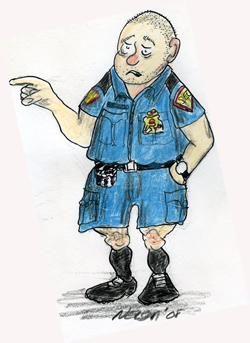
\includegraphics[height=60mm]{corps/chapitre11/img/personnage-tropecolo.jpg}
\end{floatingfigure}

Il arrive du «centre de réflexion» pour cette histoire de Saguewanish sabotée où, raconte-t-il, il a hérité d’un problème. Depuis la semaine dernière, on y héberge, sans trop de motifs apparents, un certain Robert Gagnon, pas parent avec lui soit dit en passant; lui, sa mère est une Gagnon du Témiscouata qui a épousé Gian-Maria Tropecolo, un montréalais de la Piccola Italia. Toujours est-il qu’il y a embrouille. Le dossier du monsieur semble être chez Philippe Dauphin, le directeur des communications, une procédure tout à fait inhabituelle. Or, ce Gagnon, mieux connu ici et là sous le nom épouvantable de Dart Vader, relève du 5e Nord.

- Y a rien à comprendre là-dedans.

- Faut demander à Dauphin.

- Je peux pas, il est parti jusqu’à demain.

- Qu’est-ce que vous voulez que j’y fasse ? Il m’a passé carrément par-dessus la tête, Dauphin. Il a fait incarcérer mon bénéficiaire simplement parce qu’il avait un petit peu chialé à la télé contre le Centre.

- Si personne n’est là pour justifier l’incarcération, on ne peut garder le monsieur. Il doit sortir. Comme vous êtes son CS-1, prenez sur vous pour le faire sortir.

- Je peux ?

- Ben oui, vous signez la levée d’écrou, c’est tout. On n’est pas encore retourné au temps de Louis XIV et des lettres de cachet.

Intéressant le Chinois. Pour un flic !

Une minute plus tard, l’agent se retrouve avec Timothée devant une porte de cellule en compagnie de deux armoires à glace, les frères «Papynut» et «Bluesly» Côté. Sur chaque porte de cellule, un écran HD tient lieu de fenêtre. En l’occurrence, on voit Dart Vader, écrasé sur un petit lit, en train de regarder un téléviseur fixé au mur. Tropecolo tapote l’écran et, pouf !, l’image vidéo cède la place au dossier du bénéficiaire.

- Vous voyez ici, explique-t-il au CS-1, aucun motif n’apparaît au dossier pour son incarcération. Et si vous questionnez les PapyBlues – il pointe vers les deux affreux - vous allez apprendre qu’on l’a installé ici sans avoir complété la paperasse habituelle.

- Nous autres, les boss nous ont dit d’ouvrir une cage pour mettre le bonhomme. Fait que, on l’a faite, ’stie ! Clac !

- Ça n’a pas de bon sens !

- C’est ce que je pense. On le relâche ?

- Ça va de soi, répond Timothée.

Tropecolo fait signe à Papynut, à moins que ce ne soit à Bluesly, lequel, qui qu’il soit, commande l’ouverture de la porte de son DPP. Une senteur fauve de vieillard en panne d’hygiène agresse alors les quatre employés. Effectivement, Dart Vader ne s’est pas lavé depuis mercredi dernier, ce qui ne semble pas l’embarrasser. Il s’assoit sur son grabat et appuie sur sa canule.

- Tiens, si c’est pas le chef ! Flipper a eu peur de venir lui-même ?

- Vous pouvez retourner au 5e, monsieur Gagnon, lui répond Timothée. On s’en parlera.

Tandis que le bonhomme déguerpit sans demander son reste, le CS-1 autorise la «libération» directement sur le moniteur de la porte. Taptap ding ! Il est à prévoir que Dauphin ne sera pas particulièrement heureux de l’initiative. Mais on ne peut quand même pas priver un vieillard du peu de qualité de vie qui lui reste par crainte de froisser un ego. De toute façon au point où il en est, le fils de la Maririou s’en fiche.

Les deux gardiens qui en ont vu bien d’autres, saluent leurs visiteurs et s’en retournent dans leur antre, «probablement pour y croquer de petits enfants» songe Timothée. Au même moment, une voix connue se fait entendre derrière lui.

- On se dirait dans un pays barbare.

Il reconnaît le docteur Bellavance.

- Sinistre, le sous-sol, non ? Des entrepôts de produits chimiques, des geôles, des prisonniers hagards, sales, édentés, des janissaires monstrueux, un savant fou ! Comme dans les pires dictatures ! Comment allez-vous, monsieur Tardif ?

- Euh, ça va, merci. Et vous docteur ?

- Vous ne voulez pas le savoir, monsieur Tardif, vous ne voulez pas le savoir.

- Euh …

- Un jour, vous viendrez visiter ma petite installation, juste là-bas, les grandes portes blanches. On parlera.

- Au revoir, docteur.

- Au revoir Monsieur Tardif.

En refaisant surface au rez-de-chaussée, Timothée décide de foncer, tête baissée, en direction des services techniques. Ainsi, il pourra se reconnecter aux systèmes informatisés de l’établissement. Quand on est habitué à avoir accès à tout, aux locaux, à la géolocalisation, à la téléphonie, à la messagerie, à ses horaires, à son agenda, à son aide-mémoire, à un magnétophone, etc., directement d’un gadget gros comme un bleuet, un DPP, on se retrouve lourdement handicapé lorsqu’on en est privé. Pour le moins ! Mais comme il a peine à se contenir la vessie, il bifurque par les latrines du secteur. Mal lui en prend. Au moment où, sa vidange complétée, il est en train de se laver les mains, il aperçoit dans la rangée des cubicules d’aisance que lui reflète le miroir, deux pieds nus tout recroquevillés, des pauvres pieds raccordés à de misérables jambes rougies et atrophiées par le temps.

Sans hésiter, il cogne à la porte du petit compartiment.

- Il n’y a personne, chantonne la voix de Luce Morency. C’est une erreur.

- C’est vous madame Morency ?

- Je me suis trompée de salle.

Pendant plusieurs minutes, le CS-1 essaie de convaincre la démente de lui ouvrir. Et lorsqu’il y parvient, il la trouve assise, aussi nue et perdue que lors de ses autres fugues.

- Venez, madame Morency, on va s’en aller.

- Mais il faut que j’aille aux toilettes; ici, c’est pour les hommes, je me suis trompée.

- Je comprends. Venez, je vais vous montrer le chemin.

Il l’entraîne par la main et lui ouvre la porte marquée du symbole féminin.

- Prenez bien votre temps, madame Morency, je reviens tout de suite.

Timothée entend faire d’une pierre deux coups. Il va aller aux services techniques prendre livraison de sa nouvelle boucle d’oreille et il va lancer un code magenta à l’attention du sixième. Mais sur place, manque de chance, un petit écriteau avertit que le personnel ne sera de retour qu’à 13 h 30.

- C’est pas vrai !

Miraculeusement, une préposée poussant un chariot de prélèvements et de pots d’urine, cling cling cling, vient le tirer d’affaire. Il lui fait lancer l’appel d’urgence avec son DPP et il lui demande de bloquer l’accès aux toilettes le temps qu’on descende chercher la vieille dame. Celle-ci est assise en boule le long du mur, entre les lavabos et l’essuie-mains, toute grelottante en raison de l’air climatisé. Timothée s’accroupit à côté d’elle.

- Je vous connais …

- Oui madame Morency. C’était dans le temps, au Lac-Saint-Mathieu. Vous rappelez-vous ? Vous aviez un commerce de vieilles maisons mobiles et l’École de musique vous en louait quelques-unes chaque été. En tout cas, pendant quelques étés d’affilée, quand j’étais petit, madame Morency. Celle que ma mère occupait, une roulotte tout croche et en retrait des autres à cause d’un tas de roches, immense, merveilleux, plein d’embûches – j’en avais fait mon terrain de jeu - lui servait surtout à donner des leçons aux quelques étudiants qui avaient remporté un séjour au lac.

- Le lac …

- Les soirs, parfois, mon père venait nous trouver. On allait prendre une marche jusqu’à la bergerie. Les moutons venaient me voir. Je pouvais les flatter. Ils avaient de drôles d’yeux, les moutons. Ça me faisait bien rire. Ma mère elle, elle restait à la roulotte pour pratiquer son violoncelle. Ç’a été l’histoire de sa vie, la musique. Il n’y a jamais eu de vraie place pour rien d’autre …

- Vous connaissez le lac …

La porte s’ouvre brusquement et le gros Lavoie apparaît armé d’une couverture.

- Coudon, le Motté, on dirait qu’a te courre après, la bonne femme.

- Étouffe-toi donc, gros sans dessein !

Aussitôt articulée, l’invective l’étonne encore plus que Lavoie qui n’en croit pas ses oreilles. Pour la première fois de sa vie, Timothée vient de rabrouer quelqu’un. Et pas n’importe qui, le gros Lavoie, un des pires malfrats du Centre, le copain du redoutable Pierre Monger. Il se doute bien qu’il y aura représailles, mais pour l’instant, il méprise les ricanements sournois qu’il entend et repart en direction de son 5e Nord. Comme il sort de l’ascenseur, il croise Steeve Desrosiers, son collègue CS-1 du 5e Centre chevauchant une rutilante Saguewanish flambant neuve.

- As-tu oublié la réunion ?

Timothée hausse les épaules.

- Quelle réunion ?

- La TCS.

- Et merde ! Je me dépêche.

Une fois par mois pendant une demi-journée, les chefs de section du CRG-BSL se réunissaient en un comité officiel appelé Table des chefs de section (TCS), une perte de temps d’un ennui mortel conçue, initialement, pour faire le point sur leur situation. Sauf que c’était devenu une occasion d’étaler sa supériorité, de vanter ses prouesses gestionnaires et de raconter les pires anecdotes sur les bénéficiaires. C’est de cette façon que Timothée engloutira son après-midi. Il n’aura ni le temps d’aller parler avec Dart Vader, ni d’aller rencontrer Shimoune Saint-Pierre, ni de s’occuper de sa boucle d’oreille, ni de prendre des nouvelles de sa vieille saguigui, ni de s’informer sur la viabilité de l’association Bellow – Robespierre. Par contre, en arrivant chez lui en taxi vers les 17 h, il retrouvera sa mère apparemment tirée d’affaire, fraîche et dispose.

- Marie, ton maudit chien, j’suis p’us capable !

Romain tente de frapper le chien-rat du pied, mais l’animal esquive et gronde de plus belle.

- Y est pas normal c’te chien !

- Gajou, rechte à côté de Maman, chinon, tu vas payer pour.

- J’vas aller chercher des œufs dans le poulailler.

Romain ouvre la porte de secours et gagne la petite terrasse. La brise vient chasser quelque peu la fétidité de l’air intérieur. Timothée en profite, suivi de Gazou.

- J’ai parlé à Robespierre, dit-il au travers des caquètements et des aboiements du cabot.

- Pis ?

- Il faut lui donner la lettre. Il faut lui dire toute la vérité : qui nous l’a remise, qu’est-ce qu’on a fait avec. On sait pas si le contenu est vrai, mais on pense que ça va l’intéresser. Après ça, on n’en parle plus. On la laisse faire.

- Ça marche.

- Mais c’est pas tout. Louis-Marc Richard a commencé à parler et au Centre, ils se doutent de quelque chose.

- Ça veut dire quoi ?

- Ça veut dire que je sais pas quel bord ça va prendre. Mais juste au cas où ça foirerait, garde ça avec toi.
Il lui a remis la petite bouteille de pilules.

- Y en a deux.

Sans dire un mot, sans que rien ne paraisse dans son expression, Romain enfouit le contenant dans sa poche et gagne l’intérieur où il place ses œufs sur le comptoir.

Les yeux vers le fleuve, Timothée a peine à contenir ses larmes. Il voit bien que la conclusion approche, qu’il n’est plus possible de continuer, que le «Flipper» est en train de lui faire la peau, que Richard va continuer son œuvre de délation, cette fois auprès du BAG, que le docteur Gagnon va vouloir ses médicaments et qu’il ne pourra les lui donner, que Marie-Odile va venir mettre son nez dans leurs histoires, que ses parents vont peut-être devoir avaler les petits cachets de Robespierre, sans compter le reste. Et merde !

- On devrait laisser l’air entrer, il fait tellement beau, se contente-t-il de dire.

- Tu veux qu’on ch’fasse attraper ? Ils vont nous j’entendre de la rue !

Le fils referme la porte.

- Maman, dit-il, j’ai une lettre pour toi, une lettre qui remonte 66 ans en arrière et qui vient de ta mère. T’en fais ce que tu veux, mais Papa et moi on pense que tu devrais la lire.

La Maririou regarde l’épais document et n’ose lui toucher. Timothée le dépose alors sur la petite table à côté d’elle.

- Où ch’est que t’as eu cha ?

Il lui parle alors de Béatrice Martin, une petite-fille de Rose Joncas qui était l’amie de Marceline Belzile.

- Je la veux pas, ch’maudite lettre-là. J’l’ai pas voulue dans le temps, j’la veux pas plus à ch’t heure. Qu’est-che qu’elle avait à garder cha toute cha vie, ch’te vieille-là ?

Romain ramasse le document et s’approche du rayonnage mural.

- R’garde b’en Marie, je vais la mettre ici, ta lettre. Si t’as envie de la lire, tu la lis. Timothée me l’a lue, on voulait savoir si ça pouvait te faire du mal avant de te la remettre. Là, maintenant là, je pense que tu devrais la lire. T’as eu beaucoup de peine dans ta vie, mais c’te lettre-là, si ce qu’elle raconte est vrai, ça peut te faire du bien, te donner un peu de paix. D’un autre côté, si, dans ton coeur, tu es vraiment convaincue que la lettre est de la bouleshit, tu pourras te dire que t’as eu raison de penser de même pendant toutes ces années et, ça aussi, pourra te donner un peu de paix. Me semble, en tout cas. C’est juste toi qui peut le savoir. Cela dit, je t’en parlerai plus.

En guise de réponse, elle s’empare de son violoncelle, ce qui est le signal du cérémonial. Gazou file se cacher sous un lit, Romain va quérir son trombone et Timothée, convaincu que c’est possiblement la dernière fois qu’il vivra ce rituel, en fait autant avec sa fichue de clarinette, le cœur bien gros.

- Trio pour clarinette, violonchelle et piano, opuch 2 de Vinchent d’Indy.

Une bande d’enfants déboule en trombe sur la rue Crouet. Presque debout sur leurs vélos, ils passent sans les remarquer, devant Louis-Marc Richard qui, devant sa maison, est en discussion avec deux visiteurs qui semblent s’intéresser au faux cottage obstruant la vue du côté nord de la rue. 
\chapitre{Sous le joug d’Ilsa la louve, du 25 au 26 juillet 2033}{En 2002,}{ le docteur Jawad Kebbaj, 30 ans, diplômé de la Faculté de Médecine et de Pharmacie de Rabat, prenait enfin conscience, après quatre années de tergiversations bureaucratiques à Montréal, Québec et Ottawa, que jamais il ne pourrait pratiquer l’art d’Esculape au pays de la castonguette. Le brassage ahurissant de papelards, les retours innombrables à la case de départ, l’arrogance de certaines autorités décisionnelles avaient eu raison du peu de patience dont disposait le Marocain. Comme il aimait démesurément les femmes et qu’il avait des réserves par rapport au Prophète et ses sourates, il choisit de rester et de demander sa citoyenneté canadienne, ce qui lui fut accordé en novembre 2003, malgré les suspicions nées dans la mouvance du 11 septembre 2001. }

Jawad adorait les Québécois, peuple bon enfant qui semblait associer Maroc et bouffe : «Ah, tu es Marocain ? Écoute, j’ai un tajine et je fais souvent du poulet aux olives» ou encore «Ah, tu es Marocain ? Si je te dis comment je prépare mon couscous, vas-tu rire de moi ?» ou encore «Ah, tu es Marocain ? Qu’est-ce que tu penses de l’huile d’olive tunisienne de Sfax ?» Pendant ces quatre années, il avait travaillé dur au souk Sami Fruits du Marché Jean-Talon, il avait fait des heures abrutissantes dans un dépanneur de Villeray et il était devenu chauffeur de taxi non propriétaire dans l’est de Montréal. Mais en 2008, l’amour de sa vie l’avait amené à quitter Montréal pour s’établir dans le quartier Saint-Robert de Rimouski. C’est ainsi que depuis 25 ans, il conduisait son bahut dans la métropole du Bas-Saint-Laurent. Ses clients n’ignoraient pas qu’il avait des réserves par rapport au Prophète et au Coran, mais ils savaient également qu’il ne tolérait absolument pas que l’on manque de respect ni envers l’un, ni envers l’autre. Si en 2033 Jawad Kebbaj ne portait plus le titre de docteur, Il se consolait en voyant ses fils Étienne et Xavier étudier la médecine à l’Université Laval.

- Au lieu d’un docteur Kebbaj, Soubhanallah, il y aura deux docteurs Québage, articulait-il en souriant.

Quand il observe Timothée en train d’attacher sa ceinture sur le siège arrière de son véhicule électrique, il ne peut retenir une remarque.

- Si tu continues à toujours te promener en taxi, il va falloir que je te négocie un forfait, mon jeune homme. Sinon, tu vas te ruiner.

- Bonjour monsieur Kebbaj.

- Ne me dis rien. Laisse-moi deviner. Si tu t’es mis de l’eau de Cologne, c’est que tu t’en vas chez une belle, une belle avec qui tu espères passer de bons moments, tabarnak.

Jawad se voulait Québécois tricoté serré.

- Je vais donc faire diligence, mais sans trop de brusqueries. Je ne veux pas te virer l’estomac en compote. Tu vas avoir besoin de tous tes moyens, mon jeune homme.

\begin{floatingfigure}[l]{40mm}
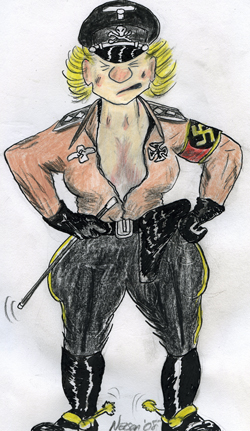
\includegraphics[height=60mm]{corps/chapitre12/img/personnage-marie-odile-ilsa.jpg}
\end{floatingfigure}

C’est avec le sourire de quelqu’un qui boit son thé en sirop ultra sucré, que quinze minutes plus tard, il dépose Timothée devant l’appartement de Marie-Odile. C’est presque en face de l’École Paul-Hubert, l’alma mater de tant d’ânes qui, aujourd’hui, s’en prennent à lui. Avoir perçu ce qui trottait dans la tête de son client, Jawad Kebbaj lui aurait sûrement servi cette perle de la sagesse ancienne, «arbat al bhim ahdha al bhim, mou’almou nhig i’almou chhig», autrement dit «si tu accroches l’âne à côté d’un autre âne, il lui apprendra à braire». Des ânes, des brutes, des éléments de troupeau, des idiots qui ne savent pas ce que c’est que de vivre en cachant de vieux illégaux sur le point d’être débusqués, qui ne savent pas ce que c’est que de marcher avec 1000 kilos de plomb dans sa poche à stress, qui ne savent pas ce que c‘est que jouer du trombone quand on déteste cet émetteur de pouet-pouet qui tue toute possibilité de découvrir l’instrument essentiel à son harmonie de vie, qui ne savent pas ce que c’est que de venir se rapporter à l’heure convenue à une femme flic pour apprendre ce que sa vie sera désormais.

Assis au salon dont l’essentiel du décor lui avait échappé l’autre soir, il remarque qu’aucune bouteille de vin ne décante, qu’il n’y a pas de musique d’ambiance et que Marie-Odile est habillée comme pour aller courir cinq kilomètres dans les feuilles d’un sous-bois. De son fauteuil où elle s’est juchée, les jambes repliées, elle l’observe comme une araignée se pourléchant devant une mouche prisonnière. Pire, comme une mante religieuse face à son petit mâle grotesque. Mais elle perçoit assez vite l’inconfort extrême dont souffre son visiteur et elle choisit d’y mettre fin. Gentillesse ? Compassion ? Magnanimité ? Félinité ?

Elle a beaucoup réfléchi, lui raconte-t-elle. Elle comprend parfaitement sa situation. Il est plus que probable qu’elle aurait agi de la même façon si elle s’était trouvée dans ses chaussettes. Les liens du cœur sont ainsi faits. Dans la vie, on peut être chef de section ou agente de sécurité, on demeure avant tout un fils ou une fille. Le sang parle plus fort que le quotidien d’une carrière. Sauf que le malheur a joué contre lui et l’a placé dans une situation intenable. Des méchants lui en veulent et ils semblent tenir un filon pour le bouffer tout cru. La vie est bien cruelle. Une jungle où les lianes se louent à la minute. Ceci étant dit, il faut se rappeler que tous les égouts mènent à la mer. Il suffit d’avoir un plan et de le suivre méticuleusement. Justement, voyez-vous, elle en a un, de plan. Un plan en quatre points avec, au terme, l’océan ensoleillé et ses effluves.

- Euh ?

Elle lui explique avoir flairé quelques maillons faibles dans l’écheveau de calamités qui caractérise l’ordinaire du pauvre garçon depuis quelque temps, le pire étant le bon docteur Gagnon lui-même. Sa faiblesse ? Il est convaincu de la tendre imbécillité du fils Tardif. Il croit le tenir à sa merci en raison des liens émotifs particuliers à la situation. C’est effectivement une belle faille et c’est par là qu’elle, l’agente de sécurité Marie-Odile Tremblay, matricule 6758AAZ-BSL-01, se glissera et réussira à lui arracher toutes ses dents. À froid.

- J’suis pas sûr de te suivre …

Se basant sur la réputation du CRG-BSL où tout n’est que carambouille, maquignonnage, imposture, crossage et vol, le médecin est convaincu que Timothée trouvera une façon de lui fournir les produits pharmaceutiques dont il a besoin. Il en a demandé cent pour être certain d’en avoir dix. Il lui suffit de savoir doser la pression, de savoir bien étirer l’élastique, de ne rien précipiter, de continuer à ne pas laisser de traces; le brave employé lui ramènera ses médicaments, petit à petit. Mais s’il se fait pincer, le brave employé ? S’il parle ? N’est-ce pas dangereux pour le docteur qui, de par la loi, est tenu de dénoncer des vieillards illégaux quand il en rencontre, ce qu’il n’a pas fait avec les parents de Timothée ? Il peut donc être accusé de complicité, n’est-ce pas ? Pas vraiment. En réalité, si cela se produisait, il plaiderait la compassion. Il dirait qu’entre ses obligations légales auprès du ministère des Affaires gérontologiques et son serment d’Hippocrate le forçant à porter secours à ses frères humains quels qu’ils soient, où qu’ils soient, sans considération lucratives, il aura opté pour la seconde partie de l’équation. Et il n’en dira pas plus sous prétexte de secret professionnel. Tant et si bien qu’il s’en tirera comme bien d’autres l’ont fait avant lui.

- J’ai vérifié et j’ai constaté que depuis l’entrée en vigueur de la loi Turcotte, le gouvernement n’a jamais poursuivi les médecins réputés avoir soigné professionnellement et gratuitement, soi-disant par compassion, des personnes louches en ce qui a trait à l’état civil. Personne ne veut se retrouver en Cour suprême.

- Mais Gagnon exige de se faire payer …

- As-tu une preuve ? Non ? Ce sera ta parole de petit fonctionnaire subalterne du MAG contre celle d’un professionnel influent qui en mène large dans certains cercles rimouskois. Tu te feras planter, ensuite, il te traînera devant les tribunaux pour diffamation. En même temps, tes parents se feront ramasser par les agents du BAG.

Marie-Odile répugnait à utiliser le mot «flic».

- Et ça, tu ne le veux pas. Il faut donc éviter que la situation en vienne là. Mais tu dois bouger vite. À la vitesse où les choses évoluent, c’est certain que tu frappes ton mur de briques d’ici vendredi. Trop de méchants t’ont présentement dans leur collimateur.

- Euh ?

Elle s’est levée et arpente énergiquement son salon.

- Écoute attentivement. La première partie de mon plan consiste à trouver une preuve que Gagnon demande un paiement illicite en retour de ses services. Tu vas donc aller le rencontrer, demain au plus tard, pour négocier un délai d’une semaine. Tu lui diras avoir une combine sûre pour te procurer ce qu’il veut, par exemple une complicité essentielle que tu es en train de développer, mais que tu as besoin d’un peu plus de temps. Soit qu’il accepte, ce qu’il fera si je l’ai bien décodé, soit qu’il refuse, ce qui revient au même. Pourquoi ? Parce que, tout à l‘heure, je vais remplacer le bouton du haut de ta chemise d’uniforme - ça tombe bien que tu ne te sois pas changé avant de venir ici – je vais te le remplacer par le mien qui, comme tu le sais, cache une microcam. Comme ça, tu pourras numériser toute la séquence. À part la couleur, nos chemises d’uniforme sont semblables. Elles sont fabriquées au même endroit et ont les mêmes boutons. Gagnon qui est certain que tu es le pire des caves ne pensera jamais que tu es en train de tout filmer.

- Oui, mais s’il a un petit bidule comme le tien pour brouiller les ondes ?

- Ça m’étonnerait ! Y a personne qui a ça à part les forces de l’ordre.

- Oui, mais ça sera un enregistrement illégal …

- Un enregistrement illégal qui ne pourra être utilisé en cour ? C’est pas pour la cour qu’on fait ça, c’est pour Internet. Il faut que Gagnon sache qu’à tout moment, on peut mettre ça en ligne. C’est une épée de Damoclès sur sa tête, quoi. C’est ce qui va nous permettre de passer à la deuxième partie du plan.

Dieu du ciel que cette femme sait organiser les choses, prendre des décisions et imposer son point de vue !

- Eh ! Oh ! M’écoutes-tu ? fait-elle en se tapant les mains. Allô la Lune ! Tu me suis ?

Elle enchaîne sur le stade suivant, lequel, estime-t-elle, est «un peu plus compliqué». Il repose sur la complicité d’une troisième personne, une personne fiable hors de tout doute, une personne qui, si jamais c’en arrivait là, ce qui serait très étonnant, témoignerait avoir reçu d’urgence, mercredi dernier, des soins confidentiels du bon docteur Étienne Gagnon moyennant juste rétribution.

- Idéalement demain soir, après-demain au plus tard, j’irai cueillir formellement son témoignage, C’est essentiel pour passer à la partie 3 du plan. As-tu quelqu’un pour agir comme troisième personne ?

- Les deux amis sur qui je pourrais compter travaillent au Centre.

- T’as sûrement quelqu’un d’autre?

Il secoue la tête négativement.

- C’est pas une réponse ! Va falloir que tu trouves. Cette personne est LA clé. La fin temporaire de tes ennuis. Du temps que tu gagnes pour mieux t’organiser.

Timothée est découragé. Tout cet échafaudage lui semble tellement tiré d’un mauvais roman policier.

- T’as vingt-quatre heures pour trouver. Après, t’es cuit. Well done ! All dressed !

Surtout que s’il y arrive, elle pourra passer à la troisième étape et faire d’une pierre deux coups. Primo, elle se pointera chez le docteur à qui elle demandera de corroborer le témoignage de la troisième personne. S’il refuse, elle le menacera avec l’enregistrement de la microcam. Secundo, elle se fera un plaisir de le regarder directement dans les yeux pour lui dire d’oublier ses produits pharmaceutiques. S’il les veut absolument, ses foutus produits, il n’aura qu’à venir les voler lui-même en déjouant tous les systèmes de sécurité ou il n’aura qu’à recruter de vrais malfaiteurs pour le faire, le Centre en compte quelques-uns. S’il râle, elle le menacera, encore là, avec l’enregistrement de la microcam. S’il devient violent ? Elle s’amusera. Elle rappelle, non sans délectation, s’être adonnée aux arts martiaux pendant sept ans. Bien sûr, elle était plus mince, mieux musclée, plus souple et, surtout, plus jeune. Mais il lui reste, disons, quelques habiletés pouvant contribuer efficacement à pacifier un toubib devenu désagréable et désorganisé.

Puis ce sera la partie 4, la plus simple du plan de Marie-Odile.

- C’est là où tu me déclares formellement que depuis ton arrivée sur la rue Crouet, ton méchant voisin d’en face n’a jamais cessé de t’enquiquiner et qu’il te déteste parce que ta maison lui bloque la vue. Je présenterai cette histoire comme une chicane entre voisins.

Timothée revoit Richard, être sournois et désagréable s’il en est, en train d’arroser sa pelouse d’un œil et de l’écornifler de l’autre.

- Quand tout cela sera terminé, je téléverserai la synthèse de cette information dans un rapport à l’attention de la direction générale. On y apprendra que mercredi dernier, tu as dépanné une personne de ton entourage, une personne qui, pour des raisons personnelles et confidentielles, préfère utiliser le secteur privé du réseau de la santé en allant chercher le docteur Gagnon, lequel a été dûment payé pour ses services, ce qui est parfaitement légal. Puis j’ajouterai des explications quant à ton idiot de voisin. Et je signerai. Ça devrait geler Dauphin et Michaud «pour quelque temps».

- Euh … et Richard, de l’autre côté de la rue ?

- Lui ? S’il veut déconner, je vais lui faire la peur de sa vie, il va nous foutre la paix !

Mais attention, insiste-t-elle. La notion de «pour quelque temps» est ici très importante. Le voisin aura beau être rationalisé, les hommes de Flipper neutralisés, il se sera dit des choses. Il y aura possiblement des traces. Des rancœurs. Et il n’y a jamais de fumée sans feu. Pourquoi Dauphin, pour le jouissif plaisir de se venger, n’enregistrerait-il pas une dénonciation anonyme auprès du Bureau des affaires gérontologiques, le BAG ? Ou pourquoi Richard ne le ferait-il pas, ou le docteur Gagnon ou un autre qui aurait pu voir passer l’information ? C’est leur devoir de citoyen de le faire, non ? Bref, il est certain que la maison de la rue Crouet va, un jour, peut-être dans un mois, peut-être dans un an, recevoir la visite des flics du BAG.

- Seigneur que c’est angoissant tout ça !

Marie-Odile, en route vers la cuisine, hausse les épaules. Timothée l’entend ouvrir le réfrigérateur, puis bardasser autour.

- Évidemment, fait-elle la tête dans une armoire à verres, ce sera donnant donnant.

Ça y est, se dit-il, voici la facture et elle ne peut être qu’étourdissante ! Mais prudemment, il évite de répondre et se place en mode attente, ce qui ne dure pas une éternité. Cabaret en main, Marie-Odile revient avec un muscadet de bonne mine, deux coupes et des biscottes. Seigneur !

- Ça t’intrigue pas plus que ça de savoir ce que j’entends par «donnant donnant» ?

- Euh …

Elle sourit largement et s’active avec le tire-bouchon.

- C’est l’autre côté de la feuille où j’ai écrit le plan que je viens de t’expliquer !

Timothée se lève pour l’aider dans sa tâche sommelière, mais il est trop tard, pop!, la bouteille a été ouverte.

- Ça va aller, tu peux te rasseoir.

Pendant qu’elle emplit les verres, elle lui rappelle lui avoir parlé, vendredi, de ses parents, deux désespérés à la veille de devoir être internés au Centre. Un bien grand malheur ! Si ce n’est pas la diète au Nutrisuz, alias le manger mou, qui les emportera en moins d’un an, ce seront les mauvais traitements et le manque d’hygiène. Il faut donc trouver une meilleure solution et, justement, elle a songé à quelque chose de potentiellement pas trop désastreux. Elle a d’abord imaginé les faire passer sur l’île d’Anticosti, mais son père n’a pas la santé suffisante; il y serait très malheureux. Elle a ensuite réfléchi sur une sorte de mise en commun. Elle, toute seule, ne peut arriver à entretenir ses vieux. Elle ne dispose ni du temps ni des moyens nécessaires. À plus forte raison que s’ils deviennent illégaux, ils perdront leurs revenus de pensions. Lui, Timothée, c’est exactement la même chose; son état actuel de détresse en est une belle preuve. La solution serait donc de tout vendre, la maison de ses parents à elle et celle des Tardif, rue Crouet, puis d’acheter «plus grand ailleurs», dans un rayon de 50 kilomètres de leur travail, en priorisant les propriétés relativement … isolées. Dans cette hypothèse, on aménagerait des espaces privés pour respecter l’intimité des gens. Mais il y a des risques. Imaginons que les deux couples ne s’entendent pas ou qu’une telle adversité leur arrive à elle et à lui.

- Pourtant, on n’a pas le choix.

La vitesse et la maestria avec lesquelles l’employée de la Sécu est en train de l’embobiner dans un cocon à sécurité maximale font frémir Timothée.

- Donc, conclut-elle, on va se mettre à l’ouvrage.

La série noire et sa liste de catastrophes continuent. Ce qui tend à démontrer qu’au moment où on croit toucher le fond, il est toujours possible d’aller plus creux. Le rationnel est pourtant simple : toute situation en dégénérescence a une vitesse de bordélisation qui équivaut à la somme des efforts consentis pour l’enrayer, multipliée par le nombre de jours écoulés depuis le début. On jurerait entendre Robespierre.

- Tu m’écoutes ?

Les yeux qu’il lui adresse sont ceux du caribou qui scrute un chasseur d’allure joviale en train de lui faire signe de ne pas bouger parce que tout va bien se passer.

- On va mettre des locataires dans ta maison, ce qui va rapporter des sous. De mon côté, je vais en faire autant avec mon condo. En même temps, je vais vendre le bungalow familial et, une fois l’hypothèque, les prêts et les frais remboursés, il devrait me rester assez d’argent pour payer «nos» coûts de réno dans la nouvelle demeure où on va aménager quatre logements : un pour toi, un pour moi, un pour mes parents et un autre pour les tiens. Chaque mois, je vais verser mille dollars dans ton compte pour que tu t’assures que personne ne manque de quoi que ce soit. En plus, je vais t’aider avec les courses. Ça va nous permettre de nous voir de temps en temps, ajoute la femme flic en clignant de l’œil. Qu’est-ce que t’en dis ?

Une fois ces lourdes responsabilités distribuées à son entière satisfaction, elle a vidé son verre d’un trait et s’est levée.

- Pis, mon plan ?

- Euh …

En moins de temps qu’il en faut à un homard pour accéder à la boette au fond de la trappe, Timothée se retrouve dans les draps de la maîtresse femme qui lui fait rapidement exulter l’exaltable. Même qu’elle le complimente sur sa prestation, une nette amélioration sur les autres fois. Si si ! Mais, il ne faut surtout pas en rester là, n’est-ce pas ? La vie est si courte. Allez, mon beau Timo ! À l’attaque ! Oh hisse ! Du nerf ! Sursum corda ! En soupirant, le pauvre diable pense à ce que doit être le quotidien du godemichet dont il aperçoit la base dans le tiroir mal fermé de la table de chevet.

- Ouille ouille ouille, mon jeune homme ! Tu as toute la luxure de l’enfer des chrétiens étampée au visage.

Timothée que Marie-Odile vient de renvoyer chez lui en taxi, non sans lui avoir rappelé les consignes du lendemain en lui remplaçant le premier bouton de sa chemise d’uniforme, regarde le chauffeur.

- Vous travaillez beaucoup, monsieur Kebbaj.

- Y a ma moukère qui dit que la vie coûte cher, tabarnak.

Quelques courtes heures plus tard, Timothée poireaute à côté de Dart Vader dans le bureau de Philippe Dauphin. Plus tôt, en arrivant à son officine du 5e Nord, il avait pris note de cette convocation d’urgence lui ordonnant de se présenter à la direction des communications en compagnie du bénéficiaire Robert Gagnon. Mais depuis cinq minutes qu’ils font face tous les deux au superbe meuble en acajou qu’utilise le Flipper pour bien camper son pouvoir, personne ne s’est encore occupé d’eux. On leur a crié d’entrer et on les a ignorés. Quand Dauphin n’est pas au téléphone, il donne des ordres à ses sbires qui vont et viennent ici et là, incluant dans la cuisinette adjacente au grand bureau. À ce que comprend le CS-1, le branle-bas semble attribuable à la réunion du conseil d’administration prévue pour le lendemain matin.

- Peux-tu vérifier qu’en fin de journée, aujourd’hui, tous les véhicules du Centre soient bien alignés dans le stationnement ? s’informe le Flipper à une adjointe à la mine peu réjouie.

- Pas de problèmes, Philippe.

- As-tu demandé à quelqu’un de faire le rappel habituel ?

- J’ai fait ça moi-même, hier soir. Ça va te coûter des heures sup, boss !

- À quelle heure les traiteurs vont venir porter leurs plats de bouffe ? crie-t-il encore à Claude Sey occupé dans le coin-repas.

- Je leur ai dit de passer entre 21 h 30 et 22 h, entend-on. C’est l’heure où le concierge vient faire le ménage; les portes sont débarrées.

Clouc ! Les yeux de Dart Vader viennent soudainement de s’illuminer.

Après un dernier téléphone et une ultime manipulation sur son terminal, Dauphin, drapé dans un costar de riche et cravaté de rouge, dévisage au travers de ses foutus binocles de soi-disant intello, ses deux «convoqués» avec tout le mépris dont il est capable et, c’est connu, son registre est très développé. Sans les saluer, il les apostrophe d’entrée de jeu. Il se dit furieux, humilié, il veut des explications, des excuses. Depuis quand un employé subalterne peut-il court-circuiter la décision d’un directeur ? Si Gagnon était en «cellule de réflexion», c’est qu’il y avait de bonnes raisons, que les intérêts supérieurs du CRG-BSL étaient en cause. Si n’importe qui commence à faire n’importe quoi dans cet établissement, rien n’ira plus. En un mot, cette histoire ne restera pas là.

- Ça vient de te coûter ta job, le cave ! Attends que j’en parle à Carl !

Timothée regarde en silence cette onzième plaie d’Égypte lui débarquer sur le bide et lui coller à la peau.

L’adjointe aux «heures sup» pointe son joli nez, côté jardin.

- La Sécu est arrivée.

- Fais-les rentrer.

Le temps de passer en revue tous les chapitres de la petite apocalypse qui l’habite depuis quelques jours, Timothée voit apparaître, côté cour, Marie-Odile et Tropecolo le Chinois.

- Vous allez me ramener ce vieux malfaiteur dans le trou d’où vous l’avez laissé filer hier, avez-vous compris ?

Tropecolo se gratte le crâne aux poils ras.

- Pour quel motif ?

- Ordre de la direction générale.

- Il est où cet ordre ? Justement, je ne l’ai pas trouvé hier.

- Laisse faire la paperasse ! Sortez-moi ça de mon bureau !

- On peut pas enfermer les gens comme ça. Ça prend un ordre signé par quelqu’un d’autorisé.

- Écoute, le Chinois, fais pas le «smatte» ! Je te dis de descendre ce vieux sac à merde et tu vas le faire. C’tu clair ?

- Moi, le Flipper, je te dis «pas d’ordre signé, pas d’emprisonnement». Rappelle-nous quand tu en auras un.

\begin{floatingfigure}[l]{40mm}
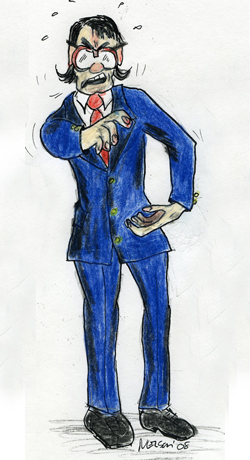
\includegraphics[height=60mm]{corps/chapitre12/img/personnage-dauphin.jpg}
\end{floatingfigure}

Il fait signe à sa collègue et tous deux déguerpissent malgré la rage évidente du satrape de la haute direction. Ce que Timothée croit décoder, c’est que les jours du Chinois sont non seulement comptés, mais qu’ils lui seront très douloureux à vivre. Idem pour Marie-Odile. Il aurait envie de cracher quelques bons sarcasmes, mais ce n’est pas dans sa nature et il se contente de donner un léger coup de coude à Dart Vader.

- Nous autres, Flipper, on va en faire autant. Tu sais où nous joindre !

- J’vous ai pas dit de partir ! Et mon nom c’est Dauphin, pas Flipper !

Dart Vader s’approche du bureaucrate et referme sa canule.

- Écoute-moi b’en, mon astie d’face de trou de cul, tu m’as fait passer six jours dans une cage du sous-sol, b’en j’vas t’le faire regretter pour le restant de tes jours ! Compte sur moi ! Tu vas apprendre qu’à mon âge, on n’a pas six jours à perdre comme ça !

Et, bras d’honneur à l’appui, le bonhomme fait volte-face et sort du bureau, son CS-1 lui emboîtant le pas.

Se pourrait-il que la vie terrestre, celle des humains, soit un divertissement adulte que s’offrent des forces inconnues, une sorte de mégajeu vidéo avec des cartes gagnantes, par exemple celle du IIIe Reich qui donne droit à quinze millions de morts ou celle de l’Encomienda à sept millions, et des cartes perdantes, par exemple celle de la guerre anglo-argentine qui ne donne même pas mille morts ou, pire, celle de l’invasion de la Grenade où il y a moins de cent décès ? Se pourrait-il que le Grand Ordonnancier qui a programmé ce jeu soit devenu cinglé ou soit couché en permanence avec une pipe d’opium collée au bec ? En attendant de résoudre cette énigme, Timothée décide de profiter de son passage au rez-de-chaussée pour se rendre aux services techniques. On ne sait jamais, se dit-il sans trop d’espoir.

Mais, à bien y penser, pourquoi lui remettrait-on un DPP tout neuf quand tellement de possibilités néfastes peuvent les en empêcher ? On a l’embarras du choix : le département sera fermé, le modèle qui lui est destiné sera en rupture de stock, une opération d’inventaire sera en cours, le préposé ne trouvera pas les clés de l’armoire, un météorite sera tombé sur le local, n’importe quoi.

Effectivement, rendu sur place, il constate que si ses appréhensions étaient fondées, il n’a pu en imaginer la raison.

- Écoute, Motté, je peux pas t’en donner un neuf, lui explique l’obèse derrière le guichet de service. C’est marqué, ici, que tu fais l’objet d’une enquête.

Il peut arriver qu’on ait la certitude qu’un disjoncteur cérébral va céder et que 43 ans de colère seront déversés sur un misérable fonctionnaire qui aura commis l’erreur d’ânonner l’imbécillité normative ultime, celle qui aura fait déborder le vase. Si c’est ce que Timothée ressent, rien ne paraît, sinon un léger agacement.

- Enquête mon œil, c’est une connerie du Flipper.

- R’garde, c’est inscrit ici. J’y peux rien. Si fais l’objet d’une enquête, on peut rien te donner; c’est le règlement. Va te «clairer» de ça et reviens nous voir !

Et shlack!, le gaillard referme le guichet, confirmant le très frustré chef de section dans son rôle de perdant venu au monde pour une tranche de pain moisi, de musicien hypersensible à qui on n’a remis qu’un méchant trombone, de Timothée de Saint-Anaclet que des parents ont confondu avec Timothée de Milet, de cave sans importance que des lèche-culs font parader dans leur bureau à côté d’un petit vieux à canule, de baiseur néophyte à qui une ancienne karatéka tetonnée accorde une note de passage, de mangeur en série de pizza qui se fait zigner par un chien laid à pleurer. Hurler ? Frapper ? Mettre le feu ? Tout faire sauter ? Ou, comme il a toujours fait, laisser «border» ?

Laisser «border» comme cette fois, c’était l’hiver, où des condisciples du Paul-Hubert, en mal de sensations fortes, l’avaient encerclé en le moquant du mieux que leur piètre vocabulaire le permettait. Redoux aidant, ils étaient plus nombreux qu’à l’accoutumée à flâner sur le trottoir entre le parc et l’école. Attaquant en meute, ils lui avaient arraché son manteau, sa tuque et ses gants. Puis, ils s’en étaient pris à son sac d’écolier, éparpillant son contenu à hue et à dia. Enfin, ils lui avaient glissé de la neige sale dans le dos, sous sa chemise.

Une kyrielle d’enchaînements injustes avait alors déferlé. N’ayant plus en sa possession le matériel requis pour suivre en classe, essentiellement des manuels et des cahiers d’exercices, tous déchiquetés sadiquement, il avait été puni par le professeur de français et expulsé par sa collègue en mathématiques. De plus, n’ayant pu leur remettre les travaux hebdomadaires entendus pour cause de dissémination aux quatre vents, incluant ceux destinés aux profs d’anglais et d’histoire géographie, il avait reçu quelques zéros et avait été consigné à la retenue du samedi, ce qui impliquait d’être reconduit à l’école par son père, le transport scolaire n’étant pas accessible les fins de semaine. Pire, le fait de devoir retourner à la maison sans vêtements chauds lui avait fait prendre froid et il avait été malade pendant une bonne semaine sans que sa mère lui permette de garder le lit comme le réclamait son état. En fait, c’est la Maririou qui s‘était alors avérée la plus terrible conséquence; sa colère avait été à la hauteur du crime. Comment se pouvait-il qu’à son âge il «perde ses affaires comme un bébé de maternelle» ? Il n’était qu’un «grand niaiseux», un «étourdi», un «immature», un «nono», une «honte pour ses parents». Comme punition, il avait été privé de télé et de dessert pendant presque un mois; Romain avait dû intervenir pour qu’elle le gracie. Eut-il dit la vérité au lieu de baragouiner de vagues «j’sais pas moi», la sentence maternelle aurait été pire encore. «T’es pas capable de te défendre, espèce d’innocent ?»

On avait bien ri au Paul-Hubert.

Timothée revoit ce barbu resplendissant de santé l’aborder, il y a deux ans, dans un centre commercial.

- Timothée Tardif ?

- Euh … oui ?

- Tu étais au Paul-Hubert en 2005 ?

- Euh … oui ?

- Je sais pas si tu me replaces ? Gilles-André Voyer, moi aussi j’étais au Paul-Hubert. Le jour où tu t’es fait attaquer, que tu t’es fait enlever ton linge et ton sac, je faisais partie de la gang. Sur le coup, j’ai bien ri. Mais le lendemain, j’ai commencé à avoir des remords. Cent fois, j’ai voulu aller te trouver pour m’excuser. Je l’ai jamais fait et je l’ai toujours regretté. Aujourd’hui, je t’ai vu arriver, je me suis dit, c’est Tardif, c’est lui. Faut que j’y aille. Fait que là, je t’offre mes excuses. J’ai agi en «sans cervelle».

Et il était reparti sans saluer, s’étant contenté de se faire du bien.

Pourquoi les autres ne l’ont-ils pas fait ? Il y en a qui exercent présentement des emplois importants où ils sont sûrement appréciés, des salauds que la vie a bien gâtés, eux. Ils ont des familles, une conjointe et des enfants qui les aiment. Probablement. Ce sont des leaders, des «influenceurs», des «battants», des «gagnants», des actifs socio-économiques, des gens utiles. Certains font même parler d’eux dans les médias. Et il y en a deux, pourtant pas les moins pires, qui sont des flics gradés du Bureau des affaires gérontologiques (BAG). Pourtant, ils se sont déjà attaqués à lui comme des hyènes sans qu’ils n’en subissent les effets pervers. Ils ont un voilier, un chalet à Métis, ils voyagent en Europe, ils sont membres du club de golf du Bic, ils ont de gros placements. Pourquoi est-ce ainsi ? Pourquoi n’y a-t-il jamais de conséquences à s’acharner sur les Timothée Tardif de la Terre ? Est-ce sa raison d’être, à lui le fils de la Maririou ? Permettre à du futur bon monde, en tout cas, à de futures «forces vives du milieu», de connaître au moins une fois dans leur vie, ce que c’est que d’être brutal, injuste et vraiment enfoiré ? Et, tant qu’à y être, pourquoi sont-ce ces Flipper Dauphin, ces Carl Michaud, ces Étienne Gagnon, ces fils de pute qui ne s’émeuvent que pour leurs petits intérêts personnels, qui finissent par faire la loi partout, qui gravissent les échelons de la société, qui aboutissent maire, député, ministre, président, qui mettent les vieux en cage sous les applaudissements de tout un chacun ? Les gentils, les doux, les honnêtes, les «qui aiment les vieux» eux, ils ont des lunettes épaisses, des bedons, un début de calvitie. Ils n’ont pas de Saguewanish, pas de boucle d’oreille et sont en train de se faire embrigader dans une relation étouffante par une femme flic, par une émule de Ilsa la louve des SS.

- Pourquoi, câlisse !

Comme un ahuri se parlant tout seul, il prend l’ascenseur sans remarquer Vlado Marcovski, le furtif directeur de l’informatique qui en sort et qui semble ravi de ne pas avoir eu à le saluer. L’eut-il vu qu’il l’aurait sans doute ajouté à sa liste des «fils de pute». À plus forte raison que depuis ce matin, plus rien ne va du côté systèmes; c’est la panne générale. Michaud doit être en train de constituer un peloton d’exécution et Dauphin, en train d’équiper une salle de torture quelque part au sous-sol.

Arrivé au 5e, Timothée consent sans trop réfléchir à une demande de Martel qui veut passer la nuit dans la «petite chambre» avec sa conjointe.

- Ronnie Ross m’a dit de voir ça avec vous, Chef.

Laissant le vieillard perplexe, il file directement chez Robespierre, sans un regard pour Jean Saint-Gelais qui veut le féliciter pour son attitude vis-à-vis Dart Vader, sans ralentir devant une nouvelle supplique de Mme Loubert concernant, cette fois, la qualité des sacs pour colostomie qu’on lui a remis la semaine dernière.

- C’est de la cochonnerie, ils coulent, vos sacs. Je suis obligée de laver sans cesse mes vieux de l’autre jour.

- J’ai pas l’temps, madame Loubert, voyez ça avec Ronnie Ross.

Occupé à pousser ses 300 pompes de la matinée, Robespierre ne dit pas un mot quand son ami entre sans frapper. Discrètement, Mme Bellow qui était occupée à compléter des fiches, quitte sans faire voir de rien.

- Je tchôque !

L’homme fort se relève et s’enroule une serviette autour du coup. Dans les petits haut-parleurs, Léo ferré chante «L’âge d’or» :

    Nous aurons la mer
    À deux pas de l’étoile
    Les jours de grand vent
    Nous aurons l’hiver
    Avec une cigale
    Dans ses cheveux blancs
    Nous aurons l’amour
    Dedans tous nos problèmes
    Et tous les discours
    Finiront par Je t’aime
    Vienne vienne alors
    Vienne l’âge d’or…

- Quelle naïveté, ça date de 70 ans, fait-il en stoppant son lecteur multimédia.

- Tu pues ! lui répond le fils Tardif qui tente de se travailler une contenance. Pauvre madame Bellow !

- Normal, je sens le neg’!

- Ouin !

- Je t’écoute.

Sans ratures ni hyperboles, il raconte au docteur Robespierre ce que, selon Marie-Odile Tremblay, il doit faire tout de suite s’il veut être encore vivant et, possiblement bien portant, dans un jour ou deux. Primo, numériser subrepticement des propos compromettants chez Étienne Gagnon, secundo, trouver une personne voulant se prêter gratuitement à un parjure. Rien que cela !

- Il est génial son plan !

Timothée le regarde, dérouté.

- Génial ! Et j’ai justement la personne qu’il te faut pour le témoignage. Et tu sais qui, d’ailleurs !

- Euh ?

- Pense ! C’est une idéaliste qui est allée organiser un dispensaire en Haïti, une infirmière qui déteste les gros requins de la médecine, une femme que le mot Nutrisuz indispose au plus haut point …

- Ta copine Béatrice qui m’a donné la lettre de Marceline ?

- Ouaip ! Comme je la connais, ça devrait marcher. Je vais t’arranger le coup après l’ouvrage. Si elle veut pas, ce qui m’étonnerait, je vais essayer de trouver quelqu’un; fais-toi z’en pas. Quant à l’autre élément de ton histoire de fous, t’as pas besoin de moi. Tu vas voir ce salopard, tu lui fais ta passe-passe et, couic, il est cuit. La seule difficulté est d’activer la caméra sans qu’il s’en aperçoive. Fais-la démarrer avant d’entrer dans son bureau.

Timothée se retient pour ne pas pleurer et esquisse un mouvement pour disparaître.

- Attends, merde !

Robespierre tape sa boucle d’oreille, demande la direction médicale et, du même ton que s’il avait communiqué avec l’assistance annuaire, s’informe des disponibilités au Centre du docteur Gagnon. On lui répond que le médecin ne passera pas avant après-demain et que, d’ici là, il est possible de le joindre à son cabinet privé.

- Tiens, prends mes clés de char, ça va aller plus vite qu’à pied et ça va te coûter moins cher qu’en taxi.

En moins d’une heure, Timothée réussit ainsi à se rendre à la clinique, à se faire introduire chez le brave docteur entre deux rendez-vous, à se négocier un délai supplémentaire pour le début de ses livraisons – il a tenté une semaine, mais Gagnon ne lui a finalement consenti que quatre jours - et à revenir au Centre où il se présente dans les locaux de la Sécurité.

Sourire aux lèvres comme s’il était l’Agent 007 lui-même, il salue Marie-Odile sans trouver de patère pour jeter son chapeau que, du reste, il n’a pas. Silencieusement, il pointe du doigt son premier bouton et, d’un geste de la tête, laisse entendre que sa pêche aux connards a été fructueuse. Si la femme flic est impressionnée, elle n’en fait rien paraître. Plutôt, elle sort un petit couteau de sa poche et lui fait sauter le bouton en question.

- Oups ! Oh ! As-tu remarqué, il te manque un bouton ?

On échange des sourires complices et le redoutable espion s’approche de la porte.

- Tu vas voir que Gagnon est très clair, il n’y a pas d’équivoque possible, sur les produits qu’il me demande de lui livrer et sur l’outil de chantage qu’il utilise pour me forcer. Pour l’autre partie, la troisième personne, c’est sur rails et je t’en reparle demain !

- Pas ce soir, minaude-t-elle ?

- Demain.

- Mais ce soir, on pourrait … tu sais … Je t’attends vers 20 heures ?

- Euh …

- File ! J’ai du travail. À ce soir.

La bonne nouvelle, Marie-Odile a l’enregistrement. La mauvaise, elle le tient du même coup. Ce qui lui fait penser, en récapitulant sa récente vie d’adulte sexuellement actif, que le prix à payer pour pouvoir tirer honnêtement son coup est très élevé. Les à-côté, les avants et les après de la partouze proprement dite sont considérables. Du temps de son holotar, la branlette de conclusion était infiniment moins lourde à supporter. Or, il paraîtrait que si on est en amour, il n’y a plus rien à endurer, ni avant, ni après, ni à côté. La relation est d’une félicité constante et l’acte sexuel ne vient qu’ajouter à l’agrément. Pour l’instant, il se trouve loin de cette image et rien ne lui indique que ce sera avec Marie-Odile qu’il pourra atteindre cet état de nirvana. Bien au contraire, tout ce qu’il entrevoit avec cette forte femme, ce sont des chausse-trappes, des barreaux de cage, des contrôles serrés, des vérifications incessantes, des miradors entourés de doberman et de rottweillers, des façons de faire auxquelles il a été habitué avec la Maririou, grâce auxquelles il a souffert et il souffre encore, avec lesquelles il ne peut plus vivre.

Sa montre lui indiquant 13 h 55, il hésite entre remonter au 5e faire face au zoo qui l’attend ou descendre au rez-de-chaussée aller voir Shimoune Saint-Pierre qui tient absolument à lui parler et dont la pause repas commence dans cinq minutes. À l’instar de Robespierre, le préposé au manger mou, alias la Grande Folle, est généralement de bon conseil. Aussi bien lui rendre visite. Mais Sébastien Larose, le dernier syndiqué de la fonction publique du Québec, l’interpelle directement de son bureau, un coqueron parfaitement inutile dont la porte est toujours ouverte.

- Aille, mon homme !

Timothée le salue de la main.

- Ça tombe bien que tu passes dans le coin. Je cherche un mot de 13 lettres qui commence par un P, qui finit par un N et p’is que la sixième lettre est un R.

- Euh …

- Ça veut dire : «Action d’améliorer unilatéralement ses conditions de travail dans les hautes sphères de certaines administrations publiques.»

- 13 lettres ?

- Oui.

Timothée compte un instant sur ses doigts.

- PRÉVARICATION !

- Aille mon homme, t’es vraiment capab’ toi ! Merci.

Avant de se faire attraper pour une nouvelle requête, le CS-1 file vers les escaliers et dégringole jusqu’à la cafétéria où il est accueilli par un regrettable «Tiens si c’est pas le beau Momo !»

- Moman que t’as pas d’l’air en forme, toi ! Tu r’sembles à un mort qui a mal ressuscité. As-tu bouffé au moins ? J’ai une glacière dans mon char avec des fruits, du fromage, des viandes froides. Y a même un litre de jus d’ananas. Je m’en allais manger ça en prenant le soleil. Ça te tente de partager ?

- Euh … je ne veux pas t’enlever le pain de la bouche.

- Mon de doux ! J’en ai en masse, s’il y en a pour un, il y en a pour deux, Momo ! De toute façon, j’ai une méchante histoire à te conter. Viens !

Le soleil étant trop violent pour Timothée, Shimoune accepte de surseoir à son rituel de bronzage. Glacière en main, tous deux s’en vont s’asseoir à l’ombre des grands sorbiers près de l’aile sud.

Mais loin de là, à l’extrémité éloignée de l’édifice, un homme a commencé à appliquer le plan qu’il a ourdi depuis le matin. Sur sa chaise de dortoir,Dart Vader, un vieux calepin sur la cuisse, est en train d’écrire au directeur général Carl Michaud, ce que ni Timothée, ni Shimoune ne peuvent savoir, occupés qu’ils sont à bien autre chose.

- T’es cuit Momo ! Les mémères qui nous observent sont déjà parties placoter partout que je m’en vais te sauter dans les buissons.

- Y a p’us rien qui peut m’écœurer, Shimoune. Y a p’us de place !

- Ouh-la-la !

- Je suis devenu un esclave, une larve, une merde. Pire qu’avant. Je suis passé du contrôle de ma mère à celui d’Ilsa, la louve des SS.

Shimoune émet un long sifflement.

- Qui c’est, Ilsa la louve ?

- Un personnage de dominatrice dans un vieux film des années 70.

- Je ne suis pas certain de te suivre. T’es quand même pas en train de me parler de la Tremblay ?

- Oui

Le préposé au manger mou pourrait répondre qu’il l’avait bien prévenu, qu’il ne fallait que s’en prendre à lui-même, que c’était couru. Mais il cache sa pensée. Par tact. De toute façon, ils ont beaucoup mieux à se dire, en tout cas, lui, Shimoune, il a de l’information qui devrait faire son petit effet.

Une fois la glacière ouverte, Le CS-1 réalise que les rations sont peu copieuses, ce qui lui en dit long sur la générosité de son ami. Son ami Shimoune, un marginal comme Robespierre, jovial descendant d’une longue lignée d’Alcide antillais. Marginal comme lui, gras du bide binoclard dont on se moque au Centre. Marginal non pas comme gai-assumé chez les hétéros, noir-fier chez les blancs, ou exclu-timide chez les grégaires, mais comme contrastant par rapport aux autres employés, tout empesés selon les diktats d’un même sale moule.

Dans les deux heures qui suivront, plus Shimoune va avancer dans son récit, plus la relative faim que Timothée ressentait va le quitter. C’est que les faits étalés changeront carrément le cours de la vie du fils Tardif. D’une part, ils lui offriront une raison pour résister aux charmes envahissants d’Ilsa la louve. D’autre part, pour la seconde fois de la journée, un ami lui fera entrevoir de la vraie lumière au bout de son tuyau d’égout.
\chapitre{Les errements nyctalopes d’une grande folle, du 22 au 25 juillet 2033}{Etre gai à Rimouski,}{ ce n’est pas l’être à San Francisco, à Vancouver ou à Montréal. À Rimouski, il n’y a pas de «village», la communauté étant étalée un peu partout dans les quartiers, dans les paroisses limitrophes et dans les petites villes avoisinantes. Il n’y a ni sauna, ni salon de coiffure, ni sex shop pour homosexuels. Si certains bars sont plus gais que d’autres, les clients «straights» y sont quand même omniprésents. Les épais également. D’où les deux heures de musculation et de boxe que s’impose Shimoune Saint-Pierre quatre ou cinq fois par semaine, si ce n’est pas plus. C’est ce qui explique pourquoi ses tenues extravagantes, voire fofolles, contrastent avec le diamètre imposant de ses biceps et la forme inquiétante de ses poings. }

Si d’aventure, il doit défendre son personnage qu’un idiot choisit bêtement d’agresser, il s’en tire toujours sans une égratignure, sauf peut-être certaines rougeurs sur les jointures après avoir fracturé un nez, ouvert une arcade sourcilière ou disloqué une mâchoire. Sa philosophie de base se résume ainsi : «Simoune oui, moumoune, non !» 

Il en est des gais comme des hétéros. Les gens sont normalement d’un ennui mortel; leur quotidien est routinier, insipide, assommant, mécanique, déprimant. Pour se désennuyer, ils regardent, de leur salon, de leur terminal, de leur télé, de leur coin de fenêtre sur la rue Crouet, la vie d’une poignée de marginaux qui eux, artistes, sportifs, malfaiteurs et autres vedettes, bourlinguent à fond la caisse. Ils la commentent et l’analysent, cette vie qu’ils épient. Ils l’aiment ou la détestent. Ils rêveront souvent de pouvoir se l’offrir, de pouvoir ainsi rechercher les sensations fortes, les histoires folles, les sauteries prodigieuses, les partouzes démentielles, les rencontres inoubliables, les voyages au bout de soi, les raids au bout de la nuit, les intoxications par substances légales ou non, les moments puissants et les souvenirs inaltérables.

L’ami Saint-Pierre, lui, il est un gai vivant. Très vivant ! Mais sauf exception, il est plutôt raisonnable durant la semaine; pourquoi indisposer inutilement son patron Amédée Chicot en entrant au boulot avec une tête de zombie, des yeux de poisson mort et l’intérieur de la bouche en plancher d’écurie ? Par contre, le vendredi soir, dès son quart de travail terminé, il va se mettre à l’affût de «gros partys débiles» et s’il en trouve, zou!, il va tout faire pour fracasser son record personnel de dérape. On n’a qu’une vie, non ? En revanche, si rien ne se passe, il va se changer les idées en alternant sa fin de semaine entre chez lui et le gymnase. Chez lui, il fera du ménage, écoutera de la musique et préparera de la bouffe, au gym il suera et gardera un œil ouvert sur les occasions. Surtout aux douches.

Quand en début de soirée, il a fait son entrée - remarquée comme toujours - à l’Errance, un bar huppé du quartier Saint-Germain, il a immédiatement repéré son ami Martin «Tintin» Arsenault, un collègue de la jaquette délirante, qui buvait du champagne avec un quinquagénaire porteur de fringues que seuls les moralement pourris qui sont socialement acceptables peuvent s’offrir. Son cerveau s’est alors mis en mode SQL et, en quelques secondes, il a identifié le bonhomme comme étant un comptable agréé de Sainte-Luce associé au parti Liberal, un dénommé Jonathan Roy. Bon père de famille, notable apprécié dans son village de banlieue, il lui arrivait parfois de venir s’acoquiner avec de jeunes hommes de Rimouski, question d’assouvir les plus secrets de ses fantasmes.

Comme Tintin lui a fait signe, Shimoune s’est approché et s’est fait offrir une coupe. Puis il y en a eu d’autres. Subodorant un potentiel d’agapes, il s’est accroché et, au bout de deux heures, c’est-à-dire quatre bouteilles de Veuve, il s’est retrouvé ami de longue date de Roy, qui, plus ivre que pompette, s’est dit prêt à passer à du plus costaud, du moins cucul.

Shimoune le regarde dans les yeux.

- Genre ?

- Genre que j’appelle un ami et qu’on se fait inviter à son party. Un b’en gros party dans une grosse cabane au Bic en face du fleuve. Y a jamais de trous du cul, seulement du monde qui ont de l’argent. On a l’astie de paix.

- Quelle sorte de monde, mon Jon ?

- Du monde qui aime la vie.

\begin{floatingfigure}[l]{50mm}
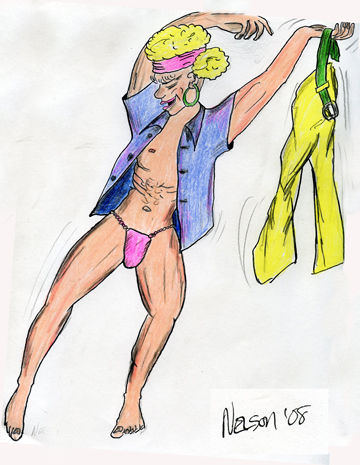
\includegraphics[height=60mm]{corps/chapitre13/img/personnage-simonstrip.jpg}
\end{floatingfigure}

Tout un euphémisme pour décrire une trentaine de bourgeois, hommes et femmes, gais, lesbiennes, hétéros, fétichistes, échangistes, exhibitionnistes et autres dépravés, n’ayant en commun que l’appartenance au parti libéral et l’argent. Beaucoup d’argent. Beaucoup plus qu’il n’en faut pour bien faire comprendre à ceux ou celles qui s’aviseraient de vouloir cancaner sur ces activités sulfureuses, qu’ils ou qu’elles le regretteraient toute leur vie quelle qu’en soit la longueur résiduelle.

La partouze a pour cadre une très grande maison construite il y a quinze ans, une construction où les matériaux dominants sont le chêne, l’érable, le cerisier et la pierre, dont les plafonds sont à douze pieds et qui s’enorgueillit d’une longue véranda vitrée et chauffée faisant face au fleuve. Pour y accéder, on doit quitter la 132 à la baie Hâtée, à l’est du village du Bic. De là, un mauvais chemin de terre serpente vers le nord jusqu’à la voie ferrée, la traverse dangereusement et continue en direction ouest pendant un kilomètre. Un stationnement asphalté apparaît alors où, ce soir, une quinzaine de voitures horriblement chères sont alignées.

Shimoune qui n’a pas assez de doigts pour compter les chambres dans le plain pied décoré de toiles, de sculptures et de tapisseries anciennes, remarque ici et là, de petites soucoupes d’argenterie pleines de cocaïne, de grands crus ouverts un peu partout, un bar étourdissant dont la spécialité semble être le scotch, des cabarets d’amuse-gueules où le caviar russe a vraiment été privilégié, une projection holographique de deux lesbiennes en train de s’aimer charnellement et deux immenses foyers hybrides à combustion contrôlée où des brasiers d’érable combattent la fraîcheur fluviale de cette douce soirée de juillet. Le mur ouest du vaste salon est une verrière donnant sur une piscine où quelques baigneurs batifolent, verre en main, dans leur plus simple appareil.

Si la plupart des gens sont habillés, certains portant des kimonos en ratine blanche, quelques-uns, pas nécessairement les plus beaux, sont nus. On s’embrasse, on se caresse, on se sourit, on s’esclaffe, on se raconte des trucs. On est seul comme cet exhibitionniste qui circule partout, le braquemart même pas au garde-à-vous, en duo comme ces fétichistes hautement bottés qui sont venus en moto, en triplet comme ce couple arrivé en compagnie d’une jeune fille du type voluptueux - Shimoune la reconnaît comme étant une des adjointes administratives de Carl Michaud, mais se garde bien d’aller la saluer – ou en quatuor comme ces deux couples échangistes qui éprouvent toutes les misères du monde à embrayer tellement l’une des deux paires est peu appétissante. Ce qu’on parvient à faire l’est au vu et au su de tous, ce qui contribue au climat général de la petite fête.

Avant que ne se présente à lui cette femme extraordinairement belle et svelte, la seule à porter un kimono noir, Shimoune, la Grande folle du manger mou, se sera adonné à différents exercices. Tout d’abord, à un indicible effeuillage au terme duquel ce qui lui sert de bobettes aura abouti, deux mètres plus loin, sur l’incontestable évidence d’un sérieux cas de priapisme. Ensuite, il se sera investi dans une session très applaudie de lutte gréco-romaine, calibre «jeux gais», où il aura pu récupérer son soi-disant slip, son adversaire étant l’infortuné porteur dudit cas de priapisme. Quant aux autres activités, contentons-nous d’imaginer qu’elles correspondaient à sa définition de «gros party débile» !

Il vient à peine de porter à ses narines une petite cuillère de poudre blanche, que la blonde, tout en grâce et en dignité, s’approche, les deux mains dans ses cheveux coupés à la nuque. De ses grands yeux verts, elle regarde Shimoune, la tête un peu inclinée. Si elle est saoule, rien n’y paraît et si elle est cokée, son calme le cache parfaitement. Elle lui déclare le trouver «magnifique et appétissant», même s’il n’est «pas complètement déshabillé», même s’il semble passablement éméché. Lentement, elle caresse, de ses longs doigts manucurés, les marques de lutte qu’il s’est infligé dans le haut des bras et, sans aucune retenue, lui annonce dans un français germanisé qu’elle souhaiterait qu’il lui «fasse des choses». Quand il lui confesse son orientation sexuelle, une condition à laquelle il n’a jamais pu déroger, elle n’insiste pas et, sans mot dire, on la dirait résignée, habituée à la fatalité, l’amène par la main jusqu’à l’autre bout du salon. Un pansu aux épaules en bouteilles semble l’attendre depuis le divan de cuir où il est langoureusement étendu.

- Ché fous présente mon mari, le propriétaire de la maison. Ça fait cinq ans qu’il ne m’a pas baisé; il ne s’intéresse plus qu’aux hommes. Moi, ché mé démerde comme ché peux. Allez, ché fous laisse, auf wiedersehen.

Shimoune connaît ce peu appétissant mollasson. C’est Pete Barrett, Pierre Barrette dans ses jeunes années, l’homme du pouvoir libéral occulte dans la région. Tout passe par ses petits doigts boudinés et sans lui, le gros Turcotte ne serait rien. On dit de cette limace baveuse qu’il n’a pas d’amis, mais qu’il est suicidaire de s’en faire un ennemi. On chuchote que Philippe Dauphin et Carl Michaud lui doivent leur poste. Idem pour cette enflure d’Amédée Chicot, le patron du centre nutritionnel.

Il est inutile ici de préciser la suite immédiate de cette rencontre. Disons, pour résumer, que malgré son état compliqué, abscons, brumeux, Shimoune pourra témoigner du fait que contrairement à ce que peut laisser croire sa dégaine obèse de puissant patapouf décadent, Barrett passera rapidement aux actes, ne s’en tiendra qu’aux actes, c’est-à-dire qu’il ne sera jamais passif au sens receveur du terme, et se montrera d’une patience vicelarde jusqu’à ce que Shimoune arrive à contrecarrer avec de sérieux rugissements, le handicap dont l’avait frappé le cocktail polytoxique absorbé depuis le début de la soirée.

À son étonnement, le gastéropode lui fait signe que c’est terminé et qu’il ne s’attend pas à se faire rendre la politesse. Presque en même temps, comme si elle avait été aux aguets, la blonde revient le chercher.

- Si fous sêtes intelligent, fous ne répéterez à perzône, entendez-fous, à perzône, qu’il zouffre de dysfonction érectile chronique. Si jamais fous parlez, si jamais fous le dites à quelqu’un et qu’il l’apprend, il fa fous faire regretter le jour de fotre naissance. Il est tré doué pour ceula.

Elle ouvre alors son kimono et, l’espace d’un instant, dévoile une vilaine cicatrice rougeâtre qui lui balafre le ventre des seins jusqu’au pubis.

- Fous savez compris ?

Shimoune en a la chair de poule. Quel porc ! Il fait jouer la rabatteuse pour impuissants à cette magnifique Allemande, ensuite il lui fait faire le panneau avertisseur.

Quelques mètres plus loin, Tintin semble en avoir fini avec Jonathan Bérubé. Le bonhomme est couché par terre et ronfle comme un quanticordi dont le ventilateur est en train de sauter.

- C’est du vin à 250 \$ la bouteille, dit-il à Shimoune , un Château Balestard à bout de bras.

- Amène-le, on va le finir. Moi ici, j’ai un Château Clément Pichon, ça doit pas se donner ça non plus.

Les deux compères se rhabillent et décident de sortir avec leur pinard de millionnaire. Le jour est en train de se dégourdir de sa nuit, les chauves-souris sont retournées se suspendre à leur plafond, les oiseaux les moins paresseux ont déjà amorcé leur jabotage et le fleuve commence à changer de couleur. La journée sera très chaude.

- J’ai amené une soucoupe de poudre.

- J’p’us capab’, répond Shimoune qui lance son verre à bout de bras.

- D’vait b’en y en avoir pour 100 \$ !

Cette fois, c’est l’assiette qui file vers la stratosphère.

- Sais-tu ce qu’on devrait faire, continue Martin Arsenault, alias Tintin, on devrait aller marcher sur les galets au bord de la mer. Il fait tellement beau.

- OK, j’te suis.

La dentelle côtière d’une parfaite irrégularité qui s’étire à l’ouest vers le Bic et Saint-Fabien, n’est qu’un jeu infini de galets parfois acérés, de récifs imposants sur lesquels il faut souvent se hisser, d’anses ténues avec leurs familles de canards, de baies minuscules qui disparaissent à marée basse, de terre-pleins en caillou ou en gros sable, avec, en avant, tantôt très près, tantôt plus éloignées, des îles grandes ou petites, et, derrière, des caps et des falaises boisées dont des cèdres et des épinettes ayant poussé tout croche au travers des roches. Le fleuve y est le maître absolu avec ses vagues crémées d’écume salée, gavées de varech et de goémon arrachés, qui, en clapotant, viennent parfois lécher la grève comme s’il s’agissait d’un câlin, mais qui parfois, avec fracas, tentent de tout démolir comme si la rage du tonnerre de Dieu voulait annihiler ce paysage antédiluvien. Ici un huard méfiant, là des macreuses qui semblent ne pas comprendre ce que font, trop près d’elles, ces quelques bernaches égarées et ces familles d’eiders plongeurs, à moins que ce ne soient des macreuses. Plus loin, occupées à brailler, des mouettes que l’on croirait libérées d’un site d’enfouissement sanitaire. Et, invisibles, parce qu’il faut pouvoir prendre son temps si on veut les apercevoir et les observer, quelques loups marins rôdent en quête de leur premier festin de la matinée.

Mais en cette journée qui s’amorce, le nez vers le vent du large, Martin et Shimoune s’intéressent à peine aux oiseaux. Et vice versa, du reste. Comme la marée descend, leur expédition s’avère moins difficile. Les passages où il faut se glisser dans un demi-mètre d’eau glaciale sont presque tous en voie de se résorber. Au besoin, les deux excursionnistes du petit matin s’entraident sans devoir parler. Une main tendue suffit. On monte, on saute, on ahane, on grimpe, on reprend son équilibre, on s’arrête le temps de souffler.

- T’as vu là-bas ? Y a un oiseau qui vient de plonger.

- Ouin, c’est un balbuzard, répond Shimoune, sûr de lui.

- B’en non, y en a p’us au Bic.

- B’en ça doit être un faucon pèlerin…

- B’en non, espèce de grande folle, ça pêche pas, un faucon pèlerin.

- J’sais-t’y moi !

D’efforts en repos, de silence en débats ornithologiques, les jeunes gens finissent par aboutir à la Pointe-aux-Anglais, face au chenal séparant la terre ferme de l’île-au-Massacre. Mais puisqu’ils sont fatigués, hébétés, mouillés, devenus peu loquaces, ils décident de s’en retourner chez Pete Barrett, question de se trouver un samaritain disposé à les ramener à Rimouski. À la différence que cette fois, crevés par leur nuit inavouable, ils le feront par en haut, en empruntant l’ancien chemin de randonnée qui traverse le bois en direction est. Le point de départ est le premier de ces trois chalets insolents qui ont été construits sur la pointe au siècle dernier. Aussitôt dit, aussitôt fait ! Malheureusement, la piste n’est plus que vaguement balisée et le trajet promet d’être aussi pénible qu’à l’aller. Tintin parle même de retourner au bord du fleuve.

Or voilà qu’après avoir contourné un énorme rocher, un pavillon du même style, mais encore plus impressionnant que la maison de Barrett, apparaît presque miraculeusement dans leur champ de vision. Construite au milieu d’une éclaircie probablement volée à la forêt par l’entrepreneur, l’habitation est entourée de pelouse, de bosquets, d’arbustes et de haies. À ce qu’ils peuvent voir, la partie avant du terrain paraît mieux nantie. Il semble même y avoir un chemin d’accès asphalté avec muret d’apparat et barrière. Plus près d’eux, c’est l’arrière de la maison qui s’offre avec une baie vitrée protégeant contre les vents salins l’immense véranda qui l’habille en totalité.

Shimoune croit apercevoir quelqu’un en train de s’y affairer.

- Y a un Bon Dieu pour nous autres, s’écrit-il. Je vais aller lui demander s’il y a un chemin facile pour se rendre chez Barrett.

En s’approchant, il remarque que les bas de fenêtres ont été ouverts afin que l’air frais du matin puisse bien pénétrer par les moustiquaires. C’est ce qui lui permet d’entendre des exclamations, des rires et un certain brouhaha. Replaçant ses cheveux de folle du mieux qu’il le peut, il monte poliment l’escalier de la véranda où, constate-t-il, il n’y a plus personne. Par contre, merci aux grandes croisées de chaque côté de la porte, il voit que ce n’est pas le cas plus loin à l’intérieur. Dans ce qu’il lui apparaît comme étant une vaste salle à manger, des gens vont et viennent, des gens apparemment arrivés à un âge avancé à l’exception d’un gaillard d’aspect jovial, une sorte d’Hercule bedonnant qu’il rencontre tous les jours au rez-de-chaussée du Centre sous la forme d’une statue en bronze, le gros Turcotte lui-même. Instinctivement, le préposé au manger mou, fif de réputation, fait le mort. S’il frappe à la porte, il sera mis en présence de l’homme fort du régime libéral. Passe encore le dysfonctionnel Pete Barrett, mais l’homophobe Sylvain Turcotte c’est un peu trop lui demander ce matin.

Au moment où il va reculer prudemment pour rejoindre son compagnon dans le sous-bois, il voit le ministre s’écrier à grand renfort de gestes avant de disparaître du champ de vision :

- Papa, maman, bonyenne, arrêtez ça. Quand on fête son soixantième anniversaire de mariage, on fait pas le ménage. On reste assis et on se fait servir. Pas vrai matante Germaine ?

- Oui cher, fait une voix stridente. Ton pére p’is ta mére l’ont b’en mérité.

Turcotte réapparaît avec, bras dessus bras dessous, un vieil homme aussi énorme que lui et une vieille dame qui joue à celle qui proteste.

- Mon oncle Lucien, avez-vous crinqué vot’ violon pour la fête d’à soir ? crie, hilare, le gros Turcotte par-dessus son épaule.

- Oui mon homme, m’a te faire souigner la baraque.

Papa, maman, tante Germaine, oncle Lucien ? Qu’est-ce que c’est que ce bordel ?

- Maman, arrête de faire la baboune. Aujourd’hui, tu relaxes, c’est ta fête, à toi et à papa ! T’es quand même pas pour annoncer que tu demandes le divorce au bout de 60 ans !

Profitant des rires puissants du ministre qui semble animer, à grand effet de bide, ce qui pourrait être un petit-déjeuner, Shimoune opte pour une retraite discrète.

Une fois dans les fourrés, il fait signe à Martin de garder le silence et de le suivre sans faire de bruit. Son plan est simple, si, côté façade, il y a une voie carrossable, c’est que des voitures en provenance de la 132 peuvent venir. Donc, en contournant par le bois pendant quelques centaines de mètres, on arrivera sûrement à un chemin d’accès sans risquer d’être vu par Turcotte ou par sa parenté. De là, il sera facile de se rendre chez Barrett.

Effectivement, cinq minutes plus tard, les deux randonneurs débouchent sur la route de desserte où il ne leur reste plus qu’à marcher une quinzaine de minutes pour atteindre la section locale de Sodome et Gomorrhe. Mais ce faisant, ils auront eu le temps de constater que deux taupins montaient la garde à la barrière d’entrée chez Turcotte. À moins que ce ne soient deux employés du cabinet de Turcotte en train de prendre l’air matinal. En y songeant bien, pourquoi faudrait-il des gardiens ? Y aurait-il quelque chose à cacher ? Et si ce sont des gardiens, ils ne semblent pas très professionnels.

- Ils n’ont pas pensé qu’on pouvait arriver par le bois du côté du fleuve.

- Qui ça ?

- Les deux gardiens.

- Quels deux gardiens ?

- Ceux du gros Turcotte !

- Le gros Turcotte ?

- B’en oui, il est là-dedans avec son père, sa mère, avec des mononks, des matantes …

- Lâche la coke, ma chouette. Les parents à Turcotte sont morts dans un accident, il y a quelques années de ça. Les médias en ont fait tout un plat.

- Je te dis que je viens de les voir !

- Ouin ouin !

Ébranlé, sa fatigue étant ce qu’elle est, Shimoune n’insiste pas, pas plus qu’Arsenault du reste. Se pourrait-il qu’il ait halluciné ? L’alcool, la coke et l’effort physique en synergie ? Pourtant !

Après avoir dormi quelque dix heures en ligne, il refait surface hanté par l’image du ministre libéral. Même en avalant ses œufs bouillis, il n’arrive pas à décrocher. N’est-ce pas à cet immonde manœuvrier populiste que le Québec doit de voir ses aînés bouffer du Nutrisuz, être encagés comme des bêtes, être exterminés pour cause d’improductivité ?

Son ordinateur a beau être une antiquité du début de l’informatique quantique grand public et son affichage cruellement dépourvu de la techno nécessaire aux présentations holographiques, il permet néanmoins la navigation vocale et le traitement simultané en 3D de requêtes multiples. En prime, il sert de système musical sophistiqué. C’est donc confortablement emmitouflé dans la musique de Gilles Bélanger, celle des hommes rapaillés de Gaston Miron qui joue en boucle, que Shimoune vadrouille un petit trois heures dans le cyberespace.

Sa première découverte troublante lui provient du GRFR (Grand registre foncier régional) qui lui révèle tous les détails légaux particuliers à cet immense pavillon que fréquente ou … fréquenterait Sylvain Turcotte. Il a été érigé en 2028, l’année du référendum et de la création des CRG, il appartient à l’État et est sous la juridiction du ministère des Affaires gérontologiques (MAG).

- Bingo, la boîte du «gros verrat»!

Construit au coût de 3,4 M\$, sa valeur foncière est actuellement de 4,8 M\$, ce qui inclut un terrain de 2,2 acres et un chemin privé de 300 mètres. Puis, une cybervisite dans les pages déclaratoires sur l’affectation des ressources immobilières du MAG apprend au fouineur que le bâtiment sert aux relations publiques du ministère, en ce sens qu’on y tient parfois des sessions de travail loin de la trépidation urbaine. Son responsable est Philippe Dauphin, cadre du MAG et directeur des communications au CRG/BSL.

- ‘Stie, le Flipper !

\begin{floatingfigure}[l]{50mm}
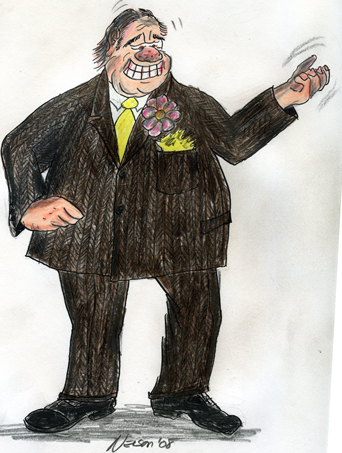
\includegraphics[height=60mm]{corps/chapitre13/img/personnage-turcotte1.jpg}
\end{floatingfigure}

Encouragé, Shimoune entreprend alors de suivre la carrière de Turcotte à la trace et, fatalement, il aboutit à cet horrible accident survenu en juin 2029 où un minibus avait fait une embardée sur la 20 à la hauteur du pont de la rivière Chaudière. Six personnes, tous membres de la famille du ministre libéral, avaient ainsi perdu la vie. Éploré, Sylvain Turcotte avait parlé de la «cruauté du sort» qui «sans préavis» privait son père, sa mère, deux de ses oncles et deux de ses tantes, «des gens modestes, sans autonomie financière même s’ils ont travaillé fort toute leur vie», de cette belle retraite qui les attendait au nouveau CRG de Rimouski, le «fleuron» du réseau institutionnel qu’il venait à peine d’inaugurer. La cérémonie funéraire avait été presque civique et les cendres avaient été éparpillées aux quatre vents sur le fleuve.

- Peuvent pas être plus morts que ça !

Et soudain, Shimoune reçoit un voyage de pierres sur le crâne. Un reportage vidéo lui présente Turcotte en compagnie de ses parents lors de la campagne référendaire de 2028. Qui plus est, Mimi Turcotte, sa mère, une femme d’allure sévère que l’on identifie comme étant la responsable régionale du recrutement des bénévoles, affirme que la campagne va très bien et qu’elle est très fière de son fils dont le projet envers les aînés va entrer dans l’histoire du Québec. Or, à quelques détails près, cette dame est exactement la même que celle qu’il a aperçue ce matin, celle qui semblait vouloir se faire tirer l’oreille. S’il avait vu juste. S’il n’avait pas halluciné. Mais depuis quand hallucine-t-on avec de la coke de riches ? Qu’est-ce que c’est que ces embrouilles ?

Et Miron de pousser dans les enceintes de Shimoune:

    - À tourmenter la nuit les vents là-haut
    les ciels poudreux d’étoiles brûlées
    où sont par ce temps mes pères et mères
    ma famille que jamais je ne revois
    et les visages peints de mes croyances

    j’erre dans la ville sans être heureux
    par rues et rafales sans hâte de dormir …

Une histoire qui n’est pas sans ressemblance avec celle des parents de son ami Timothée Tardif, une prof de musique avec un CV impressionnant et un camionneur retraité. Tous deux morts dans un incendie criminel, mais qui sont réapparus sous forme d’illégaux à la charge de leur fils. Étrange !

Une série de clips provenant de la campagne de 2019 attire néanmoins son attention. C’est le début de carrière du gros Turcotte. Il a peut-être quatorze ans de moins sur le compteur, mais il est aussi gros, aussi grand, aussi fort en gueule. Un des reportages nous le montre au sein de son comité électoral où, encore une fois, Mimi Turcotte apparaît, identifiée cette fois comme étant la directrice adjointe de l’organisation libérale du comté. On l’entend dire qu’elle a réussi à recruter des gens de qualité en provenance de tous les milieux, des artistes, des professionnels, des cultivateurs, des jeunes, des immigrants, qui viennent s’impliquer parce qu’ils sont convaincus de la plateforme progressiste et juste du candidat Sylvain Turcotte, son fils. Et parmi ces bénévoles extraordinaires qu’elle cite en exemple, elle en a justement trois près d’elle, un étudiant en sociologie, lettres et communications à de l’Université du Québec à Rimouski, Philippe Dauphin, un comptable agréé de Sainte-Luce, Jonathan Roy, et une violoncelliste de renommée mondiale, Marie Rioux.

- Attends un peu …

Shimoune aura besoin d’une quinzaine de minutes bénédictines dans les archives de l’actualité régionale avant de tomber sur l’histoire de l’incendie criminel de Saint-Anaclet. Le reportage lui semble clair. Les deux victimes sont Romain Tardif, un camionneur retraité, et Marie Rioux, la violoncelliste bien connue «dont l’incessante contribution au milieu culturel régional en fait une perte irremplaçable». Les rouages de son cerveau se mettent alors en marche, tellement qu’on croirait entendre le grincement des roues d’engrenage mal huilées. Deux tragédies violentes en deux ans, des tragédies impliquant des gens du parti libéral dont on n’a jamais retrouvé les corps. Les uns se seraient entièrement consumés dans un terrible incendie, les autres auraient été traités dans un crématorium puis dissipés sur le fleuve. Pas de trace. Sauf que, le couple Tardif-Rioux vit caché dans un sous-sol de Nazareth, Timothée le lui a dit l’autre jour à la pizzeria, et le couple Turcotte semble lui aussi bien vivant, en tout cas, il l’était ce matin dans un pavillon du Bic soustrait aux regards indiscrets dans une petite forêt rabougrie faisant face à la mer. La différence est cependant majeure. L’un vit dans la pauvreté, l’autre dans l’opulence.

Et Timothée, ce bien étrange lascar, en presque trois ans d’amitié, il ne s’est jamais ouvert sur sa vie privée que l’autre jour chez Da Peperone, probablement parce qu’il était terriblement mal pris. En fait, Shimoune ne connaît que le CS-1 marginal, peu loquace, souffre-douleur résigné, bouc émissaire statutaire, victime chronique des Monger et des Lavoie, fermé comme une huître prise sous un pilier de quai. Se pourrait-il qu’il soit au courant pour ces défunts qu’on retrouve florissants au Bic ? Ça serait logique, non ? Se pourrait-il qu’il ait une «vie secrète» ce qui expliquerait sa nature rase murs et sépulcrale ? Bref, se pourrait-il que ses parents, cette Marie Rioux et ce Romain Tardif, vivent leur quotidien au vu et au su du parti libéral et du gros Turcotte ? Car, à bien y penser, comment un chef de section si peu autoritaire, si peu apprécié, si décrié, si marginal, pourrait-il se maintenir en poste dans une institution contrôlée par des créatures à Pete Barrett, s’il n’en était une lui-même ?

Aussi bien dire que Timothée Tardif est un salaud comme les autres, mais selon toute probabilité, un salaud pris le couteau sur la gorge. Qu’est-ce qui a bien pu se produire pour qu’il ne puisse plus quérir de l’aide médicale auprès du gros Turcotte ?

- Ma belle, t’es vraiment pas faite pour un monde aussi dur.

On jurerait que Gaston Miron l’a compris.

    - Que je meure ici au cœur de la cible
    au cœur des hommes et des horaires
    que je meure ici au cœur de la cible
    au cœur des hommes

Ne reste plus qu’à confronter ce salopard. Mais, en attendant, une petite vérification s’impose.

C’est ainsi que le dimanche matin, Shimoune conduit sa bagnole jusqu’au stationnement public menant à la Pointe-aux-Anglais et à l’Île-au-Massacre. De là, il a tôt fait de grimper, de se faufiler au travers la dense végétation jusqu’au sous-bois près du pavillon et, embusqué thermos de café à la main, de se placer en mode observation. Quand il revient, une heure et demie plus tard, il a acquis deux convictions. Primo, il n’a pas eu la berlue hier matin. Mimi Turcotte, la femme des clips de nouvelles, fréquente ce pavillon. Grâce à son DPP (dispositif personnel polyvalent), il vient même de la photographier à plusieurs reprises. Par contre, le gros Turcotte ne s’est pas montré; Shimoune ne l’a ni vu ni entendu. Secundo, les deux soi-disant gardiens à l’entrée sont à leur poste, même si le ministre ne semble pas s’être présenté. La probabilité qu’ils soient de simples employés prenant l’air du matin s’estompe donc un peu. Encore là, le DPP a été mis à contribution.

Dès son arrivée au Centre le lendemain, le préposé au Nutrisuz tente de joindre son plus que probable faux frère. Il lui laisse même un message laconique, «j’ai de l’info qui pourra t’intéresser». Mais toute la journée, Timothée joue au chat et à la souris. Se doute-t-il de quelque chose ? Comme il fallait s’y attendre, la partie ne sera pas facile.

Le mardi avant midi, alors qu’Amédée Chicot est en train de l’éplucher, «putain de gonzesse, c’est pas de la graisse à pédale, ça, c’est du Nutrisuz !», Claude Sey se présente à la cafétéria.

- Avez-vous un instant, monsieur Saint-Pierre ?

- Oui mon beau p’tit pit, si tu veux voir Shimoune, tu vas le trouver. Qu’est-ce que je peux faire pour toi, mon chou ?

Chicot les regarde tous les deux avec haine.

- Tous les lopettes, nom de Dieu !

Shimoune s’est approché du comptoir.

- S’il vous plaît, monsieur Saint-Pierre, arrêtez votre cirque, vous et moi sommes assez intelligents pour nous en passer.

- C’est comme tu veux, mon p’tit chéri. Mais cesse de m’appeler «monsieur» et de me vouvoyer. J’ai pas la scoumoune, même si j’m e nomme Shimoune ! Ça me met la chaiiiiirrrr de poule aux burrrrrnnnnes.

\begin{floatingfigure}[l]{40mm}
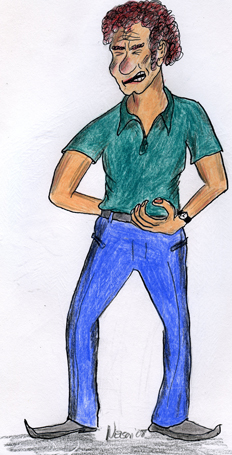
\includegraphics[height=60mm]{corps/chapitre13/img/personnage-claude.jpg}
\end{floatingfigure}

Sey hausse les épaules et raconte tout ce à quoi il vient d’assister dans le bureau de Dauphin : Timothée, Dart Vader, Tropecolo et la violente colère du Flipper.

- Pourquoi que tu me contes ça ?

- Parce que tu es ami avec Timothée et que Dauphin va vraiment se venger. Il a déjà contacté Michaud. Ces salauds sont capables de tout. Ton copain est dans une merde pas possible. Avertis-le et essaie de l’aider à prévenir les coups.

- Comment ?

- Je peux pas trop parler, mais il y a comme un début de piste, le docteur Bellavance.

- Bellavance ? C’est quoi le rapport ?

- Peut-être que s’il voit Timothée être obligé de se défendre contre cette chienlit, il aura le goût de lui dire des choses.

- Quelles choses ?

- Je peux pas t’en dire plus.

Shimoune est sceptique.

- Sérieusement, pourquoi tu viens me dire ça ici, à matin, ma belle p’tite crotte ? Si tu travailles pour le Flipper, t’es aussi pourri que lui non ? Et là en plus, tu viens me le dénoncer. Qu’est-ce qui me dit que tu n’es pas en service commandé ?

- R’garde, tu fais comme tu veux. Je t’ai raconté dans le détail ce qu’il venait de se passer. Si tu me crois pas, questionne Tropecolo, Marie-Odile Tremblay ou monsieur Gagnon. Tu peux aussi aller vérifier ici, en bas, en demandant aux Papyblues. Ceci étant dit, le comique, essaie de ne pas trop t’étouffer dans ta parano de sniffeuse de poudre cheap !

Bouche bée, Shimoune regarde filer Claude Sey.

Et il le restera jusqu’à sa pause de quatorze heures quand Timothée viendra le chercher. En attendant, il tentera de refaire le point. Au terme, son amitié aura pris le dessus sur sa méfiance. Car si son copain est un pourri, s’il est une des créatures de Barrett et du gros Turcotte, comment peut-il prendre le parti d’un vieillard diminué, ayant déjà «un pied dans la tombe», contre Dauphin et Michaud ? Et comment pourrait-il avoir tenu ces propos sur le vieil informaticien, jeudi dernier, lors de la séance du Comité de déontologie ? Est-ce la raison pour laquelle la bande à Turcotte n’entend pas l’aider avec les graves ennuis de sa mère et qu’il doive faire affaire avec le docteur Gagnon ? Est-ce parce que Timothée voudrait prendre ses distances par rapport à l’organisation libérale ? Hum !

Mais d’un autre côté, il se peut aussi que l’équation Mimi Turcotte – Marie Rioux ne soit pas bonne, que ces similitudes ne soient que fortuites, qu’il n’y ait aucun rapport entre le squat de la rue Crouet et le pavillon reclus du Bic. Et c’est connu, des vieux qui sont planqués pour se soustraire aux CRG, il y en a des masses. Si ce n’était pas le cas, il n’y aurait pas les flics du BAG, cette SPCA spécialisée dans le ramassage de vieux. Aussi bien dire qu’il est tout à fait malhonnête de vouloir établir un lien entre ces deux histoires. Les seuls faits qu’on peut vraiment invoquer sont que, d’un côté, il y a Turcotte, sa famille qui échapperait aux CRG en étant cachée dans un bâtiment relevant du MAG, le Flipper et Michaud qui trempent dans cette sale combine, enfin Pete Barrett qui a l’œil ouvert et le bon, ensuite que, d’un autre, il y a Timothée Tardif qui se saigne pour dissimuler ses parents, qui a une mère malade, qui en arrache avec un profiteur du système et qui ne sait plus à quel saint se vouer.

Si tel est le cas, il n’y a plus lieu de confronter ce pauvre diable. Pourquoi l’ennuyer avec des histoires de libéraux qui bafouent leur propre loi ? Mais il l’a soupçonné. Sans compter que sa mère a été associée à l’organisation de Turcotte. Puis, quelque part, le Momo ne lui dit pas tout. Rien n’est moins limpide que ce paquet d’embrouilles; il y a anguille dans les bobettes. Et maintenant qu’il l’a prévenu qu’il avait de l’info pouvant l’intéresser, il aurait l’air étrange de reculer, de tourner son appel téléphonique en plaisanterie, en erreur. Sans oublier cette histoire avec le docteur Bellavance, le sinistre fermier hormonal. Le mieux est sûrement de tout lui raconter, au Timothée, y compris sa suspicion. Un ami que l’on soupçonne un instant du pire et à qui l’on ne se confesse pas d’avoir ainsi pensé, n’est probablement déjà plus un ami, mais une relation mondaine.

- Tiens, si c’est pas le beau Momo, fait-il en le voyant se pointer à la porte de la cafétéria. Moman que t’as pas d’l’air en forme, toi ! Tu r’sembles à un mort qui a mal ressuscité. As-tu bouffé au moins ? J’ai une glacière dans mon char avec des fruits, du fromage, des viandes froides. Y a même un litre de jus d’ananas. Je m’en allais manger ça en prenant le soleil. Ça te tente de partager ?

- Euh … je ne veux pas t’enlever le pain de la bouche.

- Mon de doux ! J’en ai en masse, s’il y en a pour un, il y en a pour deux, Momo ! De toute façon, j’ai une méchante histoire à te conter. Viens !

Les regardant s’en aller, Amédée Chicot se tape la boucle d’oreille et demande la Direction des communications.

- Allô ? J’aimerais parler à Philippe Dauphin.

- C’est à quel sujet ?

- Putain de ta mère, connasse ! Tu lui dis que Chicot a de l’info pour lui, merde, et que ça urge !
\chapitre{Grande bouffe pour Dart Vader, le 26 juillet 2033}{Si on en croit Charles Baudelaire,}{ homme de lettres naguère fort respecté, le mal se ferait sans effort, naturellement, par fatalité et le bien serait toujours le produit d’un art. Pourtant, cette perle de sagesse ne s’applique presque pas dans le cas de Robert Gagnon, maigre vieillard trachéotomisé et édenté surnommé Dart Vader, ce qui fait de l’aphorisme baudelairien un sophisme au lieu d’un truisme. Car pour faire le bien qu’il a choisi de faire, entendre ici «châtier un méchant», le bonhomme a décidé de faire le mal, un mal prémédité et planifié. Quant à la fatalité, si elle a été de la fête, elle ne s’est pas retrouvée à l’origine de ce mal calculé, mais dans son exécution qui s’est brutalement soldée par une conclusion aussi dramatique qu’accidentelle - la vie nous réservant bien des surprises – c’est-à-dire une fin en queue de poisson incarnée dans un plat de crevettes écaillées, cuites et aromatisées à l’ail. }

En début de journée, lorsqu’il a été subir les foudres haineuses de Philippe «Flipper» Dauphin en compagnie de Timothée, son chef de section, Dart Vader a pris bonne note du fait qu’en fin de soirée, on livrerait des plats qu’un traiteur avait préparés pour la réunion du Conseil d’administration du lendemain. Claude Sey, le plus jeune des adjoints de Dauphin, a même précisé l’heure de la livraison, soit entre 21 h 30 et 22 h, moment précis où le concierge vient faire le ménage, ce qui signifie que les portes seront ouvertes. Dans l’esprit de l’ancien noceur de toutes les galères et de tous les tabacs, il ne fait alors aucun doute que le trésor festif sera apporté dans la cuisinette attenante à la salle du Conseil. Dans sa vieille tête malfaisante et rusée, il ne lui reste plus qu’à trouver le moyen de s’approprier une telle merveille. Pas seulement pour faire bombance, mais pour foutre une pagaille monstre dans l’organisation du Flipper. Il fera en sorte que l‘on sache partout que grâce à l’incurie de Dauphin, lui, Robert Gagnon, misérable avaleur de Nutrisuz depuis trois ans, il a pu se livrer à une orgie alimentaire mémorable à même la bouffe de ces salauds du CA.

Le plan qu’il se met dès lors à mijoter sera cousu de fil blanc et d’impondérables, mais il aura le mérite d’être simple. Tant et si bien que Gagnon va l’appliquer à la lettre. Depuis qu’il est pensionnaire au CRG-BSL, il a observé au hasard de ses promenades dans l’établissement – ce qu’on a fini par lui interdire - que la circulation au rez-de-chaussée commençait à se faire rare dans l’heure qui suit la fermeture de la cafétéria et qu’aux alentours de 21 h, il n’y avait plus personne dans les parages, sauf d’éventuels gardiens en Saguewanish. Sauf, également, un préposé à l’entretien qui vient passer l’aspirateur, épousseter ce qui peut l’être, vider les corbeilles et ramasser le pire dans les bureaux et les salles.

C’est ainsi qu’à 21 h, Vader emprunte les escaliers et, reprenant héroïquement son souffle à chaque palier, descend lentement vers le rez-de-chaussée. Il estime qu’en utilisant l’ascenseur, il attirerait davantage l’attention des autorités. Bien sûr, il se sait filmé, mais si on le remarque, ce ne sera que le lendemain quand on soumettra les enregistrements de la soirée et de la nuit à un logiciel de reconnaissance et identification du mouvement (RIM). Ça, c’est le bonhomme Asselin qui le lui avait expliqué l’an dernier.

Rendu en bas, il observe et écoute attentivement. On dirait un rongeur flairant les traces de renard. Convaincu que rien ne bouge ni ne respire, il se glisse furtivement sur sa droite, à la manière d’un ectoplasme, et, les doigts croisés, gagne la toilette des hommes sise de biais, en face de la salle du CA. À l’intérieur, il s’assied dans un cubicule la tête dans les mains et les coudes sur les cuisses. Le bonhomme vient de se placer en mode attente. Mais au préalable, il a accolé sur la porte un écriteau bricolé plus tôt indiquant que cette cuvette était en dérangement. Si jamais quelqu’un entrait, il grimperait sur le siège pour ne pas qu’on lui remarque les jambes; il aurait normalement le temps de le faire puisque les «visiteurs» seraient empêtrés avec leur trottinette. Sauf si c’était le balayeur. Et advenant qu’on veuille quand même pénétrer dans son cubicule, il se ferait dénoncer, ce qui lui vaudrait – il l’acceptait d’avance - un nouveau séjour dans les geôles des Papyblues. Mais, basta ! 

\begin{floatingfigure}[l]{45mm}
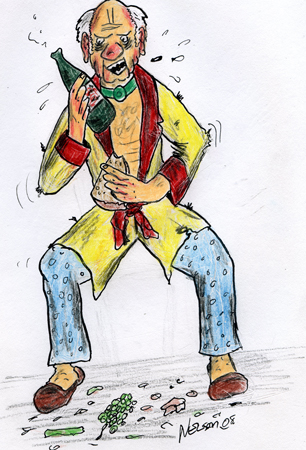
\includegraphics[height=60mm]{corps/chapitre14/img/personnage-vader-bouffe.jpg}
\end{floatingfigure}

Aux cinq minutes à partir de 21 h 30, Dart Vader va écouter à la porte, se risquant même à l’entrouvrir pour tâcher très discrètement d’observer aussi bien le concierge que les livreurs. Il ignorait alors quelle tournure la suite prendrait, mais il misait sur le fait qu’il pourrait peut-être se glisser à l’insu de tous dans la salle du CA et de s’y cacher sous la grande table. Car il y a toujours une grande table, n’est-ce pas ? Faut-il rappeler que son plan était truffé d’impondérables ?

À 21 h 40, un taupin arrive juché sur un chariot électrique et, avec vacarme, arrête son antiquité mal rafistolée devant la porte de la salle suprême. Par la magie de sa boucle d’oreille, il donne le code de la porte laquelle, comme celle des quarante voleurs d’Ali Baba, s’ouvre silencieusement. Sans se douter que des yeux affamés le surveillaient, il y entre avec tout son barda et commence son ménage. Puis, au bout de quinze minutes, il migre dans la cuisinette attenante où il poursuit sa mission hygiénique. C’est à 22 h 07 que deux porteurs de cabarets fermés se pointent en se racontant des trucs du métier qui laissent Dart Vader de glace; par contre, il passe à un poil de défaillir tant leur traînée odoriférante lui apparaît paradisiaque, appétissante, violente, sensuelle, capiteuse, irrésistible. C’est tout juste s’il ne bondit pas leur arracher les contenants.

L’homme de ménage les accueille selon les règles de l’art viril.

- Commençait à être temps, j’suis à veille de tout barrer ! Il me reste rien que le bureau du boss Dauphin à faire !

En déposant sa pile de cabarets, un des livreurs esquisse une excuse.

- Ils se sont aperçus que le céleri faisait pitié. Y ont dû le changer. C’est pour ça qu’on est un peu serré.

- Ouin, ouin !

- Là là, on a encore un voyage de cabarets, p’is on a fini.

- J’en ai pour cinq minutes, répond le concierge en ouvrant la porte séparant la cuisinette du bureau du Flipper, précisément comme elle l’était au moment de l’engueulade du matin.

À ce moment, trois actions se produisent en rafale. Les livreurs se dépêchent vers la sortie, le préposé à l’entretien fait partir son aspirateur chez Dauphin et Dart Vader quitte les toilettes pour se glisser dans la salle du CA. S’il avait encore des doutes sur l’existence d’un Dieu pour les anciens ivrognes et fumeurs extrêmes, ils sont alors annihilés. Car la table du CA est non seulement gigantesque, mais elle dispose sur toute sa longueur, d’une quille de soutien, une médiane en bois foncé qui bloque toute vue ou communication de «dessous de table» entre participants vis-à-vis. Fébrile, le vieillard file se dissimuler à l’autre extrémité du long meuble en acajou, le nez sur la pointe de la quille. Si les livreurs entrent avec leurs contenants, son plan est de se cacher à la droite de l’immense panneau ligneux et si le concierge repasse dans la pièce, il se glissera vers la gauche. Dans les deux cas, l’angle de vision sera obstrué. C’est précisément ce qu’il fait. Les traiteurs reviennent se débarrasser de leur fardeau sans rien remarquer et lancent une vague salutation au préposé qui, à son tour, réapparaît dans la grande salle où, une fois son chariot ramené dans le couloir, il éteint l’éclairage et verrouille la porte.

L’entendant rouler vers les bureaux du fond, le vieux sacripant se relève péniblement en s’appuyant des deux mains sur la table de conférence. Il a réussi ! Il est maintenant enfermé jusqu’au lendemain matin, à moins qu’il ne parvienne à sortir sans se faire attraper. Mais de cela, il doute sérieusement. Un capteur le cafarderait aussitôt qu’il arriverait à ouvrir la porte. Et là, crac ! Au trou ! Bof ! Il a déjà vu pire ! Pour l’instant, le vieillard famélique est seul avec une quarantaine de grands cabarets-contenants pleins de nourriture infiniment troublante. Comme il savait qu’en mettant l’éclairage, il ne faudrait même pas cinq minutes avant qu’un gardien de sécurité ne vienne en vérifier la cause, il s’était alors apporté une halogène à piles, ces torches bonnes pour cinq heures une fois rechargées, qu’il avait «empruntée» au poste de garde du 5e Nord.

Avant de céder à ses envies insupportables, il sort de sa poche intérieure deux feuilles de papier et un tube de colle hydrofuge. À petits pas, il passe dans la cuisinette où il doit se faire violence pour ne pas bondir sur le réfrigérateur, puis il continue dans le burlingue de cette canaille de Flipper. Comme il l’a deviné, ces portes ne sont jamais verrouillées. À l’aide de sa lampe, il colle un des documents écrits à la main, comme au temps des stylos bille, sur le bureau de Dauphin et retourne dans la salle fixer l’autre sur la table du CA, à l’endroit même où siège le président du conseil. Ils devront gratter longtemps avant de pouvoir les enlever. On peut y lire :

    Parce que tu es incroyablement con, Flipper, tu m’as permis de savoir, ce matin quand tu voulais tordre le règlement pour me retourner en prison, qu’il y aurait du vrai manger, ce soir, dans ta cuisinette, à quelle heure on viendrait le porter, le manger, et à quelle heure il n’y aurait plus personne pour m’empêcher de tout le bouffer. Ça fait que je vais bâfrer tout ce que je peux et ce que je ne pourrai pas, mettons que ça arrive, je vais le cochonner pour ne pas en laisser à ta gang de crosseurs du CA. Et comme je te truste pas, que t’es un faux jeton, Flipper, j’ai utilisé le terminal du quanticordi dans le salon communautaire du 5e Nord, pour expliquer à Carl Michaud avec copie conforme à des journalistes et à Thierry-Ian Dennis-Dubeau, le politicien qui aime pas le manger mou, que je crevais de faim dans tes cages à chiens et que pour manger autre chose que de la cochonnerie de Nutrisuz, j’avais dû voler la nourriture du Conseil d’administration. Ce qui fait que tu es en beau joual vert après moi et que je serai sûrement emprisonné à nouveau. À l’heure où tu lis cette feuille, les Papyblues sont probablement déjà en train de se limer les dents. J’ai horodaté le message pour qu’il parte une heure avant que tu entres dans ton bureau. Bye-bye et bonne journée mon cave !

Et comme un prêtre à qui on a interdit de célébrer la messe pendant trop longtemps, le père Gagnon s’approche du réfrigérateur, vaste tabernacle où on a entreposé la manne céleste, et, salivant comme un danois affamé devant un étal de boucher, il transporte tous les récipients dans la grande salle, les plaçant sur l’autel qu’était devenue la table du Conseil. Ensuite, méticuleusement, il les ouvre un à un, jetant les couvercles à bout de bras. Il découvre ainsi une véritable corne d’abondance faite d’amuse-gueules (olives, choux-fleurs, céleris, concombres libanais, cerises de terre, tomates en grappe et biscottes tartinées de foie gras) avec leurs contenants de sauce trois fromages, de la salade choux - carottes râpés au raisins secs, du taboulé, du jambon melon, du saumon mayonnaise, un monceau de petites crevettes de Matane avec un plat de sauce chili, de la confiture d’oignons à l’ancienne, un plateau complet de fromages (morceaux de cheddar blanc et orangé montés en cubes sur mini brochettes, bleu aux relents affolants, gouda en boulettes de cire rouge, emmenthal bien croûté et camembert bas de gamme), un cabaret gorgé de caramboles en tranches, de noix, de raisins verts, de figues et de poires naines, enfin un dernier plat où sont cordés des carrés de gâteaux secs, des tartelettes à l’érable et au coulis de fraise, ainsi que des biscuits à l’amande. Sur le comptoir à côté du frigo, il a remarqué un sac gonflé de petits pains et six bouteilles de Châteauneuf-du-pape, un cru de 2024, dont il a vivement dévissé tous les bouchons et les a ajoutées au désordre gastronomique de la table.

Dans une de ses poches de robe de chambre, il trouve un petit lecteur musical, le truc bête à dix sous où, l’an dernier, il s’était amusé à se télécharger tout sa musique. Il se l’ajuste aux oreilles et, du bout du doigt, navigue jusqu’à Jean-Pierre Ferland. Clic, c’est fait. La fougue du vieux barde lui emplit les émotions.

    Avant de m’assagir
    Avant de jeter l’ancre
    De ménager mon cœur
    De couver ma santé
    Avant de raconter
    Mes souvenirs à l’encre
    De vouloir sans pouvoir
    De compter mes lauriers
    Avant cette saison
    Avant cette retraite
    Je veux sauter les ponts
    Les murs et les hauts bords
    Je veux briser les rangs
    Les cadres et les fenêtres
    Je veux mourir ma vie
    Et non vivre ma mort

Alors, calmement, comme un amant qui se retient d’exulter trop tôt dans une prestation prometteuse, il s’assied, sourit d’aise et entonne le premier chant de sa grande messe. Il s’agit de crudités, dont des tiges de céleri et des pommettes de chou-fleur, ces légumes qu’il engloutissait de façon compulsive quand il était gamin, avant qu’il ne devienne l’ivrogne impénitent qu’il fut envers et contre tous. Sa prothèse dentaire enfilée, il pose, fou de désir, ce geste lourdement codé dans son ADN, geste d’un réconfort sans bornes et qu’il n’a pu oublier en trois ans de manger mou, consistant à se placer un bâton de céleri entre les dents, d’en suçoter le jus, de le croquer bruyamment, de le mastiquer avec délectation et de l’avaler.

    Je veux vivre en mon temps
    Saboter les coutumes
    Piller les conventions
    Sabrer les règlements
    Avant ce coup de vieux
    Avant ce mauvais rhume
    Qui tuera mes envies
    Et mes trente-deux dents
    Et si je le pouvais
    Je ferais mieux encore
    Je me dédoublerais
    Pour vivre comme il faut
    Le jour pour ce qu’il est
    La vie pour ce qu’elle vaut
    Ça c’est mourir sa vie
    Et non vivre sa mort

Malgré l’orgasme, malgré Ferland, il est étonné de la sensation déplaisante qu’il ressent aux gencives. Pour la première fois en trois ans, ses dents artificielles viennent de forcer, de travailler. Aucunement inquiet, Dart Vader poursuit sa marche vers le paradis avec un morceau de chou-fleur. Même désagrément sous les dentiers, additionné cette fois d’un début de tiraillement dans les masséters, ces muscles masticatoires atrophiés pour cause de non-usage. Dans le plat, tout à côté, que lui présente son halogène, il remarque une quantité folle de noix, une des grandes passions de sa terrible vie. Il a tôt fait de s’en mettre une poignée sous la dent. Mais dès qu’il commence à les broyer, la douleur lui devient insoutenable et il doit tout recracher. Inquiet, quelque peu frustré, il plonge la main dans le cabaret de jambon melon et, cette fois, il ne ressent presque pas de pression aux gencives et c’est à peine si ses muscles lui font sentir leur état de déchéance. Pour qu’il en soit autrement, il va devoir y aller à deux mains et se fouler la cavité buccale comme s’il s’agissait d’un moulin à viande. Mais sa fatigue masticatoire devient telle qu’il se fixe au bec le goulot d’un Châteauneuf et qu’il se sert du précieux liquide pour avaler ce qu’il n’a plus la force de mâcher.

- ‘Stie qui est bon, c’te rouge-là !

Et voilà le père Gagnon en train d’écluser pour la première fois en trois ans, un de ces nectars qui, en synergie avec bien d’autres, lui ont fait perdre, tout au long de sa trépidante vie, femmes, emplois et possessions matérielles. Le vieil homme tente ensuite quelques exercices en s’étirant les maxillaires. Puis, le gosier à nouveau empli de rouge papabile, il s’empare d’une pièce de saumon. Il essaie de ne pas trop l’écraser de son râtelier, mais une douleur du fond de la bouche, là où commence l’œsophage, lui témoigne d’une certaine intolérance envers tout ce qui est plus structuré que le Nutrisuz. Prenant une pause de quelques secondes, il repère le taboulé. Une forte pulsion l’entraîne alors à s’y plonger la tête comme un clébard abandonné, une manœuvre déplorable qui lui fait frôler l’étouffement. D’un geste brusque, il propulse le met fautif sur le tapis et, au passage, attrape les fromages. Il taponne d’abord le bleu et, le jugeant assez mou, s’en emplit la trappe à malice. Quelle extase ! Quels souvenirs ! À nouveau, une sérieuse rasade de vin et, derechef, une généreuse poignée de bleu. Comme dans le bon vieux temps ! Éventrant le sac de petits pains «sour dough» de style San Francisco, il en défait un en trois et, comme pour communier, s’en place un morceau dans la bouche.

- Bleu blanc rouge, grince-t-il de sa canule.

Après une pause pipi dont il confie le cadre au bureau de Philippe Dauphin, il continue son festin cette fois avec les biscottes qu’il se contente de lécher pour n’absorber que le foie gras. Et comme il sent que le conduit stomacal va lui exploser, il vide presque le quart de sa bouteille et entreprend de malaxer le tout avec force bruits de succion et de déglutition. C’est à ce moment qu’il aperçoit le plat de crevettes, un des rares mets pour lesquels il aurait tué du temps où il ne s’appelait pas Dart Vader. Il a tôt fait de se purger la bouche sur le siège voisin et d’y engouffrer une solide poignée de crustacés sans même les plonger dans la sauce rouge. Les misérables crevettes ont tellement été cuites et trafiquées qu’il n’est nul besoin de les mastiquer. Il suffit de les arroser de Châteauneuf.

- ‘Stie que c’est bon !

Mais au moment où il s’apprête à s’offrir un troisième service des deux mains, d’étranges sensations commencent à attirer son attention. Des sensations de lourdeur en progression, de picotement croissant dans les extrémités, d’étau en train de se resserrer sur ses côtes, sur ses poumons et sur son cœur, d’air qui ne parvient plus à passer. Presque en panique, le bonhomme s’empare d’une petite brochette de cheddar, se débarrasse vivement du fromage et introduit le bâtonnet dans sa canule qu’il croit obstruée. Du sang gicle alors de la trachée.

Son dernier geste avant qu’il ne s’écrase sur les cadavres de biscottes léchées, sera de s’arracher la canule.

Mais tout cela, Timothée ne le saura qu’au matin et, surtout, quelques jours plus tard quand le docteur Prévost aura pu terminer son travail.

Pour l’instant, il vient de quitter Shimoune qui doit reprendre son boulot et s’en retourne au 5e avec une nouvelle certitude en tête. Il se passe quelque chose de répréhensible au Bic, quelque chose d’explosif et de mortel pour une carrière de politicien, et sa mère, la Maririou, connaît probablement la fine fleur impliquée dans cette histoire. Elle a travaillé à la première élection du Gros Turcotte, d’où la lettre de cette enflure accrochée sur un mur du sous-sol de la rue Crouet. S’il est vrai que les géniteurs Turcotte ne sont pas morts, pourquoi, eux, vivent-ils dans un paradis sous l’aile d’un ministre omnipuissant, alors que son père et sa mère à lui, Timothée-Milet Tardif, croupissent dans la misère noire sur le bras de leur nono de fils ? Tout autre que lui imaginerait dès lors un plan visant à prendre ces accaparateurs la main dans le sac afin d’en tirer des bénéfices pour ses propres parents; car, il y a sûrement quelque chose à faire. Le problème, c’est qu’au moment où Dieu a distribué le talent de stratège aux humains, le pauvre garçon était malheureusement dehors en train de réparer la crevaison que des voyous venaient de lui infliger.

C’est madame Loubert qui le tire de sa réflexion.

- Ronnie Ross dit qu’il n’y a pas d’autres sacs et que va falloir que je m’habitue aux nouveaux.

Ça n’a aucun bon sens !

- Vous dites que les nouveaux coulent ?

- Oui et ils me salissent toute !

Aucun, mais aucun bon sens !

- Venez avec moi, madame Loubert.

Dans son bureau, il tape sur la fonction téléphonique de son terminal et demande les Approvisionnements.

- Direction des Approvisionnements ! fait une voix ménopausée.

- Timothée Tardif, 5e Nord.

- C’est à quel sujet ?

- Au sujet de votre dernière batch de sac à colostomie, ils coulent.

- Un instant, je vous communique avec un agent de procuration.

Quinze secondes de silence suivent où madame Loubert n’ose même pas parler.

- Adrien Dumont, comment puis-je vous aider ?

- Timothée Tardif, 5e Nord.

- Ah, le Motté ! Qu’est-ce qui se passe ?

- Il y a des problèmes avec votre dernière batch de sacs à colostomie, elle est de mauvaise qualité et les sacs tendent à couler.

- P’is ?

- B’en p’is ? Ça fait du dégât et j’ai une patiente qui se plaint.

- Va falloir qu’al endure, on n’en a pas d’autres !

Deux petits fils se touchent alors dans le crâne du CS-1.

- Comment « qu’al endure » ! C’est pas une réponse, ça !

- B’en c’est celle que j’te donne, le Motté !

- Écoute-moi bien, câlisse, si d’ici demain je n’ai pas reçu ici, au 5e Nord, une caisse de sacs de la même qualité qu’avant, je ramasse les pleins de marde qui coulent et je descends te les vider sur ton bureau ! As-tu compris ?

Debout dans le cadre de porte, Ross voit son chef hurler pour la première fois.

- Demain au plus tard, vocifère ce dernier par-dessus les protestations d’Adrien Dumont.

Et il raccroche.

- Motté, Motté, wouo, du calme !

Le CS-1 regarde le préposé.

- J’le connais, moi, Dumont. Si tu cries après, Motté, t’auras jamais rien. Laisse-moi faire, je vais descendre te négocier quelque chose.

- J’m’en câlisse de ce que tu vas faire, Ronnie ! J’exige seulement qu’il me monte une caisse de sacs normaux.

- J’te dis que j’m’en occupe. Tu vas l’avoir ta caisse.

Timothée qui se doute bien de la motivation profonde de Ronnie Ross, n’a aucun doute que madame Loubert pourra compter, demain au plus tard, sur des sacs de qualité. Il sait que Ross est en gamique avec quelques salauds du Centre, dont Adrien Dumont, et il a la conviction, sans les preuves, que son employé a trempé de façon profitable pour sa poche, dans cette livraison de sacs défectueux. Son intérêt est d’empêcher à tout prix qu’un CS-1 quelconque s’énerve, fasse des vagues et agite la fourmilière, ce qui pourra n’être que défavorable à ses affaires.

- Timothée Tardif, bougonne-t-il à son terminal qui vient de lui transmettre un appel.

C’est Claude Sey qui lui apprend avoir été suspendu sans solde, immédiatement après une visite d’Amédée Chicot chez Philippe Dauphin.

- Mon congédiement est désormais une formalité.

- Euh …

- Vous êtes probablement le prochain, monsieur Tardif. Pensez au docteur Bellavance.

Il a raccroché. Qu’est ce que c’est que cette histoire avec le sinistre chercheur du sous-sol ? Le personnage est un peu abject, non ? Car utiliser des corps cliniquement morts pour produire des hormones est une pratique affreuse très discutable. En quoi est-ce que ça pourrait le concerner, lui ce chef de section abusé, ce fils accablé, ce Casanova dérouté, ce binoclard grassouillet dont les cheveux tombent comme des samares à l’automne ? Y a-t-il un rapport entre cette étrange recommandation de Sey et l’affabilité dont l’inquiétant médecin fait habituellement preuve à son endroit ? Pas plus tard qu’hier, il l’a invité à venir visiter sa «petite installation» du sous-sol, celle qui est voisine de l’antre des Papyblues. «On parlera», a-t-il dit.

- J’adore ta madame Bellow, fait la voix de Robespierre derrière lui.

Timothée regarde sa montre.

- Il est 16 h 15; il arrive quoi pour ta copine Béatrice Martin ?

- Elle nous attend chez elle vers 19 h 30. Mais, oh, ce n’est pas ma copine, c’est une amie. Quelqu’un de très bien que tu vas avoir intérêt à connaître.
Comment faire pour être chez Béatrice à 19 h 30, obtenir d’elle ce dont il a besoin pour neutraliser le docteur Gagnon, demeurer poli, tout en étant, une demi-heure plus tard, chez Marie-Odile à l’autre bout de la ville ? La matrone a en effet précisé qu’il devait se pointer à 20 h. Va donc falloir qu’il lui téléphone pour se dégager une plage temporelle suffisante. Quand on sait qu’il y a une semaine à peine, Timothée n’avait jamais pu s’approcher du charme féminin, il y a de quoi s’étonner de le voir maintenant en situation de négocier avec l’une pour pouvoir aller chez l’autre.

- Faut vraiment que j’y sois ?

- Qu’est-ce t’en penses, idiot ? Je passe te prendre chez toi à 19 h. Et, sans te mettre sur ton trente-six, enlève au moins ton uniforme de garde vieux.

En route vers l’ascenseur du personnel, le chef de section songe que son ami a parfaitement raison. Il devrait faire des efforts vestimentaires, au moins quand il se présente chez les gens, surtout lorsqu’il s’agit d’une dame qui vit seule, une très belle femme toute mignonne qui dégage tellement de douceur, d’empathie, de chaleur et de bonté, qu’on en tombe instantanément amoureux. Évidemment, il y a la fatalité, celle qui oblige le rêveur à quitter impérativement son monde onirique pour se concentrer sur la vraie vie, sur ce à quoi il a eu droit, sur son lot, sur cette forte femme qu’il redoute de plus en plus, sur cette femme-flic que l’on surnomme ici la Bitch à Tremblay, sur cette mégère qui lui a ordonné de venir se rapporter à 20 h.

Deux vieux, main dans la main, le saluent.

- Je voulais te remercier pour la petite chambre, chef. T’as pris pour moi contre eux autres. T’es quelqu’un de bien !

- Je n’ai fait que mon travail, monsieur Martel.

L’homme hoche de la tête d’un air entendu et poursuit son chemin. Robespierre est impressionné.

- C’est bien qu’on te dise des choses comme ça, non ?

Mais Timothée ne répond pas. Car, au sortir de l’escalier, dans le no man’s land séparant son service du 5e Centre, Luce Morency vient d’apparaître.

- Et merde !

- C’est la madame du 6e …

- Oui. Va me chercher une couverture, veux-tu Robespierre ? Et envoie un code Magenta au 6e Nord.

Comme si tout était normal, le CS-1 s’approche en souriant de la démente.

- Comment allez-vous, madame Morency ?

La vieillarde le regarde longuement, la mine profondément angoissée, l’air totalement perdu.

- On se connaît ?

Il la prend par la main et la ramène dans la cage d’escalier où il s’assied sur une marche après lui en avoir fait faire autant.

Dans la seconde qui suit, Robespierre réapparaît.

- J’ai envoyé le code Magenta, mais je trouve pas de couverture.

Son ami hausse les épaules et, calmement, sur le ton de la confidence, amorce un énième monologue avec à la vieille dame.

\begin{floatingfigure}[l]{30mm}
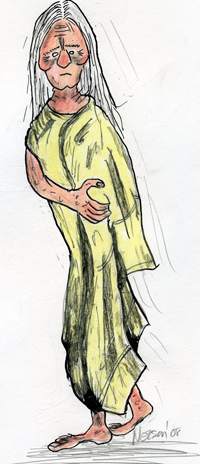
\includegraphics[height=60mm]{corps/chapitre14/img/personnage-morency.jpg}
\end{floatingfigure}

- Vous rappelez-vous au Lac Saint-Mathieu, madame Morency, cet été où il y avait eu une petite fille appelée Julie ? Une petite fille que vous aviez présentée à ma mère comme étant votre nièce de Montréal ? Une petite fille maltraitée que vous aviez accepté de garder pour l’été ? Elle était toute menue, presque maigre. Ses yeux était immenses, bleus comme le ciel quand il fait doux, le printemps. Ses cheveux étaient longs, raides et dorés comme de la corde de chanvre. Et son visage, son visage, je ne me souviens plus de son visage. Ma mère lui avait montré à jouer de l’harmonica, à déchiffrer des partitions.

- Julie …

- Oui, Julie. Elle était tout le temps avec ma mère. Tout le temps. Et elle ne me parlait jamais. Ça me chagrinait un peu parce que j’en étais amoureux, amoureux fou comme en sont capables les petits garçons. Je me cachais sous la roulotte pour la regarder pratiquer sa musique à bouche sur la petite galerie. Je pense qu’elle le savait, mais elle ne faisait voir de rien. Au fil des jours, nous nous étions développé une complicité tacite où j’étais devenu, je pense, un voyeur dissimulé dans la noirceur et elle, une belle que l’on observe furtivement.

- Julie …

- Quand nos vacances se sont terminées, elle a continué de venir chez nous, à Saint-Anaclet. Des fois, madame Morency, vous nous l’ameniez un lundi matin et vous passiez la reprendre le vendredi soir. Pour mon plus grand malheur. Un jour, vous n’êtes plus revenues et je n’ai jamais su ce qu’elle était devenue. J’ai longtemps pensé à elle en rêvant qu’elle arriverait chez nous, qu’elle me tendrait ses bras, qu’elle me dirait vouloir être mon amie. Puis, un jour, je me suis fait à l’idée qu’elle ne reviendrait jamais. Vous vous rappelez de Julie, madame Morency ?

- OK Motté, on la ramène, fait Alain Santerre, un préposé du 6e Nord qui se présente avec une couverture blanche. Merci de t’en être occupé.

Julie, un de ses plus beaux souvenirs d’enfance. Julie dont il n’a jamais su le nom de famille. Morency ? Julie Morency ? Non, cette combinaison ne fonctionne pas. Qu’a-t-elle fait de sa vie ? S’en est-elle sortie ? Elle aurait aujourd’hui 43 ans. Peut-être se souvient-elle de lui. De leur complicité ? Peut-être que s’il la recherchait et la découvrait, qu’elle lui tendrait les bras et qu’elle lui dirait vouloir être son amie ?

Cinq minutes plus tard, les deux compères roulent vers Nazareth. Avec le dispositif personnel polyvalent, alias la boucle d’oreill, de Robespierre, Timothée rejoint Marie-Odile-la-dévorante et lui explique avec douze paires de gants blancs qu’il ne pourra être chez elle à 20 h en raison de sa démarche auprès de cette Béatrice Martin, amie de Robespierre prête à témoigner dans le bon sens de cette histoire épouvantable. La femme-flic trouve la nouvelle plutôt fâcheuse, mais elle dit comprendre la situation. C’est le prix à payer, n’est-ce pas, si on veut se sortir d’un engrenage qui ne peut que nous broyer. Ceci étant dit, en experte de ce genre d’intervention, elle estime qu’il aura besoin d’une heure tout au plus et, en ajoutant trente minutes de voyagement, qu’il pourra être chez elle à 21 h, ce qui est quand même acceptable. Mais à supposer qu’il faille plus de temps, qu’il faille tout expliquer, persuader, négocier, il faudrait prévoir un filet, non ? Pourquoi ne pas s’enlever du stress et s’entendre, disons, pour 22 h ? Ce n’est pas si tard, 22 h !

- B’en on avait dit 20 h, p’is là c’est rendu à 21 h et tu veux qu’on mette ça à 22, gronde Marie-Odile. Tant qu’à y être, pourquoi pas à demain matin ? Écoute donc, es-tu sûr que c’est pour son témoignage que tu vas voir c’te femme-là ? Ne non ! 21 h, c’est une bonne heure; tu vas avoir le temps de tout faire ce que tu as à faire.

- Euh …

- Je t’attends. Travaille bien ! À tantôt mon gros loup !

«Mon gros loup» ? Dieu du ciel ! Il se sent plutôt chèvre accrochée à un piquet, lièvre dans un habitat de martre, gnou en train de courser contre une femelle guépard, carpe dodue dans un bassin à piranhas, voire hamster se sentant observé par une grosse couleuvre. Le couvre-feu est à 21 h, qu’elle a décrété, la maîtresse femme! Cela parce qu’elle entend se faire sauter à 21 h 05 ! Ce qui signifie que lui, il devra être en mode service-service dès 21 h 04. Le mode d’emploi est très simple, chère madame. Vous appuyez ici, c’est le bouton B, et instantanément l’appareil tombe en état de bandaison. Il vous suffit alors de le manœuvrer à votre convenance jusqu’à votre point G. C’est garanti ou argent remis; signez ici sur la ligne X.

Tout cela à cause du docteur Gagnon ! Et pendant ce temps-là, la mère du gros Turcotte, elle, elle doit sûrement se faire soigner aux frais de la princesse, peu s’en faut par ce salopard de Gagnon, sans que son fils ne doive jouer de trombone, sans que personne ne doive culbuter de femme-flic ou de femelle guépard ou de mante religieuse. Elle est où, la justice ?

Quand Robespierre le dépose chez lui, il aperçoit Louis-Marc Richard en conversation avec deux types dont la mine patibulaire tient davantage du flic que du malfrat. Tous trois sont collés sur la clôture qui fait face au fleuve, au bout du cimetière qui jouxte le gîte des Tardif. Ils semblent s’intéresser à l’endroit où est située la terrasse-poulailler-clapier du sous-sol, laquelle, heureusement, ils ne peuvent contempler en raison des arbres qui leur en masquent la vue. Quand Richard aperçoit Timothée, il baragouine quelque chose et, immédiatement, les deux lascars font semblant de ne pas dévisager le grand noir assis dans la voiture électrique et le binoclard bedonnant qui viennent d’en sortir.

- T’as vu ces malfaisants, Robespierre ?

Le colosse s’extirpe de sa sous-compacte.

- C’est qui ?

- Je te présente mon voisin d’en face, c’est le plus laid des trois. Il est en train de cafarder à mon sujet. Les autres, ce sont deux flics, probablement des créatures au Flipper, si ce n’est pas des salopards du BAG.

Robespierre devise l’hybride sombre stationné devant la maison de Richard.

- C’est à vous, le char ? leur crie-t-il.

Un des deux flics, ou pseudo-flics, opine.

- Ouin, pourquoi ?

À la vitesse de l’éclair, l’arrière-petit-fils de l’inventeur du Petepano fait virevolter un immonde glaviot dans le pare-brise.

- C’est parce que la vitre est sale. On dirait qu’il y a un morviat de neg’.

Tandis que les visiteurs s’en reviennent à la course, Robespierre file avec sa voiture et Timothée entre chez lui, presque souriant. Un instant, il songe à Marie-Odile qui a promis de venir donner une bonne frousse à cette mocheté d’indic, puis il descend au sous-sol familial. Il a tôt fait de réaliser que la Maririou lui tient rigueur de son retard; la rituelle pratique musicale n’a pu avoir lieu. Tellement qu’elle laisse cette sale bête de chien-rat japper, gronder et essayer de mordre aussi bien le mauvais fils que le père ronchonneur.

- Maman, te souviens-tu quand j’étais petit, il y avait eu un été où tu avais enseigné la musique à une petite fille qui s’appelait Julie ? Tu sais, elle restait chez Luce Morency. Sais-tu ce qu’elle est devenue ?

Pour toute réponse, la vieille dame se lève et disparaît dans la cuisine suivie de son bestiau. Timothée est conscient qu’il n’y a plus rien à en tirer. Idem pour Romain qui fait semblant de regarder la télé. Alors, il décide de regagner son appartement, mais avant, il s’approche de cette lettre du gros Turcotte que la Maririou a épinglée au mur, une missive officielle qui lui est spécifiquement adressée en tant que professeure à l’École populaire de musique. Le paragraphe central attire son attention :

    Parmi les bénévoles qui ont rendu possible mon élection comme député de Rimouski et, ultérieurement, mon accession au cabinet, vous avez été une des plus efficaces et j’en serai éternellement reconnaissant, peut-être pas à vous, mais au projet qui vous tient tant à cœur, l’École populaire de musique. Vous m’avez en effet convaincu de prendre partie et cause pour le sauvetage et la relance de ce bastion culturel solidement implanté dans notre région depuis plus de 35 ans. Croyez-moi madame, l’École a désormais un gardien zélé au Conseil des ministres.

Gardien zélé ? L’École a dû fermer ses portes en 2021 faute de financement public.

Béatrice Martin apparaît à Timothée encore plus belle, plus agréable et plus douce qu’il y a deux jours. Tellement qu’il arrive à peine à parler.

- Mon ami Timothée a une méchante histoire à te raconter, ma Béa, celle d’un fils qui n’a pas voulu laisser tomber ses parents malgré tout et celle d’un employé du Centre qui croit que les vieux méritent d’être respectés. Dans les deux cas, ça fait de lui un hors-la-loi et un lépreux. Bref, il est dans une merde pas possible. Mais, heureusement, tu peux l’aider.

- Mon Dieu, c’est excitant cette histoire !

- Timothée, tu veux la lui raconter ?

Lentement, avec plein de ratés au démarrage, le fils de la Maririou entreprend le récit de sa situation et il n’omet aucun détail, si ce n’est, en bonne chattemite, la nature honteusement intime de sa relation avec Marie-Odile Tremblay. Au passage, il note l’œil de l’infirmière qui s’enflamme lorsqu’il aborde le chapitre du bon docteur Gagnon.

- Autrement dit, cette policière voudrait que je lui déclare officiellement que c’est à moi et à votre demande, monsieur Tardif, que le docteur Gagnon est venu porter des soins d’urgence.

- Une saloperie que tu aurais attrapée en Haïti, ajoute Robespierre.

- Mais, euh, vous n’aurez pas de précision à apporter; la nature de votre malaise n’intéresse pas l’enquêteuse et n’apparaîtra pas dans son, euh, rapport.

- Est-ce que j’aurai à prêter serment ?

- Non, c’est une simple déclaration à une agente de sécurité du CRG-BSL.

Béatrice s’avance dans son fauteuil, déplie ses jambes recroquevillées et les pose par terre. Son beau visage devient terriblement sérieux.

- Je vais le faire, dit-elle en s’ébouriffant légèrement sa chevelure d’ébène, les yeux presque en colère. Je vais le faire pour le plaisir de vous aider à coincer ce profiteur.

Timothée laisse percevoir un soupir. Le scénario de Marie-Odile se déroule à la perfection.

- Merci beaucoup, madame Martin.

Elle le regarde de son visage redevenu serein, calme et doux.

- Vous pouvez, tu peux, m’appeler Béatrice, ça serait plus simple.

Le cœur veut lui défoncer la cage thoracique.

- Euh …

- On voit pas ça souvent, un homme mature aussi timide que toi, Timothée, rajoute la coquine du haut de son vertigineux donjon.

Qu’attend la belle Rapunzel, pour lui dérouler sa chevelure afin qu’il puisse grimper la rejoindre ? Oh qu’il s’en saisirait à pleines mains ! Rapunzel, ô Rapunzel, laisse choir tes longs cheveux !

- Euh …

Or, elle le fait ! Blou-lou-lou-lou, la mirifique tignasse dégringole jusqu’en bas, jusqu’à ses pieds. «Grimpez, beau prince !» semble-t-elle lui dire.

- Écoute, si tu veux, je peux aller la visiter ta mère, voir comment ça se passe dans son bedon, prendre sa pression, vérifier des trucs, la déstresser.

- Je te l’avais dit, mon ami. Béatrice est un cœur sur pattes.

La façon dont elle lui répète être très heureuse du fait qu’il ait pensé à elle pour essayer de se sortir de son injuste malheur, allume chez Timothée une conflagration d’espoir. Et c’est presque en flottant qu’il regagne la rue, son camarade l’observant du coin de l’œil en souriant d’une oreille à l’autre.

Comme il a préféré de pas lui confier qu’il s’en allait au logis de Marie-Odile, il le laisse le déposer chez lui.

- Hé-hé-hé !

- Quoi «hé-hé-hé» ? rétorque Timothée.

- Juste «hé-hé-hé».

- Ça veut dire quoi, ça ?

- Je me comprends.

- T’es con Robespierre. Salut !

Il lui faut maintenant aller poinçonner chez sa geôlière et il se pourrait qu’il soit en retard. En retard pour aller s’emmerder à tirer son coup ! Un regard vers sa montre lui indique qu’elle s’est arrêtée. Pile morte ? Mécanisme foutu ? Association de pensée avec sa boucle d’oreille, sa Saguewanish et son automobile ? Conjuration inexplicable ? Tout est possible.

- Saloperie !

Sur le moniteur de son quanticordi, il titille le bouton Taxi et court à la salle de bain se laver les dents. L’hygiène malgré tout !

- Ouille ouille ouille, mon jeune homme ! Tu me dis rien. Tu me laisses deviner. Attends ! Tu t’es encore mis de l’eau de Cologne, t’as des fringues propres, donc, tu t’en vas veiller dans le coin du Paul-Hubert, non ?

- Bonsoir monsieur Kebbaj, vous avez bien deviné.

- Moi je te dis. Je me mettrais du parfum comme toi, ma moukère elle me frapperait sur la tête, sur le cou, sur le nez, partout, avec son balai. Boum ! Boum ! Boum ! Elle serait sûre que j’aurais batifolé dans mon taxi. Heureusement, je n’y pense même pas ! Masha’Allah ! Mais toi, tu es jeune. Tu peux.

Sur l’écran ACL du taximètre, l’heure indiquée est 21 h 23.

- Elle est bonne votre heure, monsieur Kebbaj ?

- Si elle est pas bonne, mon jeune homme, leur satellite de merde il est maboul.

Donc, Timothée est en infraction. La taulière lui en voudra sûrement de ce retard.

Effectivement, quand il arrive cinq minutes plus tard, elle le laisse entrer sans effusion, ni chaleur, ni sourire, ni rien. Par contre, elle parle.

- J’aime pas les surprises.

- Euh …

- On avait dit 21 h et là, il est et demi ! Tu penses-tu que j’ai rien que ça à faire, moi, t’attendre ? Ça donc bien pris du temps, ton histoire avec la bonne femme ?

Le pauvre galant revoit, l’espace d’une nanoseconde, la longue chevelure de Rapunzel glissant sur les pierres du donjon, une chevelure devant laquelle, lyre en main, il a mis un genou à terre.

Une demi-heure plus tard, l’acte est néanmoins consommé et, le coude sur l’oreiller, elle lui raconte comment, demain, elle ira cueillir la déposition de Béatrice Martin et comment, cette fois avec force détails, elle ira neutraliser le docteur Gagnon. Timothée est loin de sourire. Il sait parfaitement bien que par ce geste, il deviendra inféodé à cette terrible femme, emprisonné dans ses bras musclés, jouet dans ses cuisses bouillantes, avec comme potentiel d’évasion, une probabilité moindre que celle de gagner un gros lot de plusieurs millions à la loterie.

Au moment où elle lui place la tête entre ses gros tétons, quelque part plus au nord de la ville, au rez-de-chaussée d’un édifice redouté, Dart Vader amorce sa Grande Bouffe …
\chapitre{Timothée craque et remet ça ! le 27 juillet 2033}{L'air de ce petit mercredi de semaine}{ est doux, caressant, aromatisé de tout ce qui, plus au sud, affole les bourdons, les abeilles et les colibris. On voudrait s’y intégrer, s’en faire un linceul, flotter sur son calme courant, se fondre dans la générosité de sa tiédeur veloutée, y rêver sans craindre que le bien-être ne cesse même en se tenant tout près du fleuve en défiant la vigueur des débris salés. On souhaiterait s’encoconner sans retour dans le confort de ce matin de juillet, se perdre dans ces draps de satin blanc, ceux de la nuit incessante, «Nights in white satin, Never reaching the end … », des draps au lyrisme plus prenant que celui de cette froide cotonnade enrobant le vilain trébuchet par où il a fallu passer. Car on aimerait oublier avoir dû sacrifier sa soirée au plus désagréable des stupres, dans la plus angoissante des geôles.  }

On aimerait oublier avoir le cou bien étiré sur une bûche, avoir une meute de chacals déployée tout autour pour la curée, avoir ses proches en grand péril, être en train de naviguer dans un épais cirage sans trop d’instruments fiables. En revanche, on a des amis, peut-être même une amie, sur qui il est possible d’apprendre à compter, si on le veut Pas si mal quand on est un tromboniste involontaire n’ayant pas encore trouvé de passage, aller simple, pour Milet, un binoclard, bedonnant, en chauvaison, recalé socialement. Chauvaison ? Lorsque la calvitie frappe, on tend à se développer un vocabulaire pour en qualifier le processus.

\begin{floatingfigure}[l]{35mm}
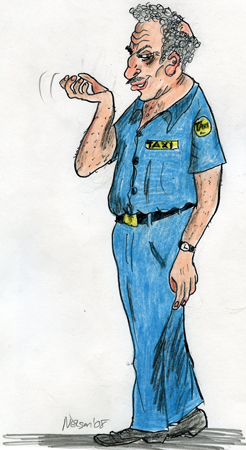
\includegraphics[height=60mm]{corps/chapitre15/img/personnage-jawad.jpg}
\end{floatingfigure}

Entre l’improbable cottage de la rue Crouet et l’immeuble du CRG-BSL, il y a exactement huit feux de circulation. Or, c’est la première fois, depuis qu’il fait ce métier, que Jawad Kebbaj franchi tous ces portails au vert, «Masha’Allah» !

- Il faut prier en initié, mon jeune homme !, dit-il à son rétroviseur à grand renfort de clins d’œil.

Effectivement, à chaque feu, l’ex-médecin marocain psalmodie la formule incantatoire, formule un peu adaptée, mais remontant néanmoins à la nuit des temps, formule qu’auraient utilisée pharaons, dignitaires et nobliaux en quête d’un siège pour que cesse leur errance postmortuaire. Dit-on.

- Laisse-moi passer, feu de circulation, je te connais et je connais ton nom, je connais le nom du dieu qui te garde. Tu t’appelles «Souverain de la peur, aux hautes murailles, le supérieur, souverain de Hebhed, le prophète qui repousse la tempête, qui sauve de la spoliation celui qui vient de loin», ton portier se nomme «le Redoutable» et le dieu qui te garde s’appelle Osiris.

Puis :

- Laisse-moi passer, feu de circulation, je te connais et je connais ton nom, je connais le nom du dieu qui te garde. Tu t’appelles «Souverain du ciel, maître du double pays, l’avaleur, souverain des hommes, contrôleur de tous», ton portier s’appelle «le Rejeton de Ptah» et le dieu qui te garde se nomme Osiris.

Et ainsi de suite, autant de portails-feux, autant de suppliques, autant de permissions divines, autant d’invraisemblances qui contredisaient la conviction de Jawad à l’effet qu’il était mathématiquement impossible de les franchir tous dans la félicité du mouvement continue. Oriris, le dieu aux quatorze morceaux, n’avait-il pas décentralisé la gestion de ses portails, laissant une grande latitude aux portiers, des créatures pas toujours accommodantes envers les humains ? Mais aujourd’hui, tout semblait surréaliste. Par exemple, qui eut cru possible de connaître un matin aussi doux que ceux de Rabat, quand les ardeurs du soleil de juillet sont rafraîchies par la brise de l’Atlantique et les effluves du fleuve Bouregreg ? Mais voilà, tout est concevable en ce bas monde, même la douceur, la joie de vivre et ;e répit. N’en a-t-on pas la preuve en ce début de journée ?

Descendu de la voiture, Timothée remarque une dizaine d’employés, toutes des jeunes femmes, assises, souriantes, heureuses, le nez pointé vers le soleil, comme ces personnages peints sur papyrus dans le Livre des morts. Il s’attarde un instant en ce sérail impromptu, se tourne lui aussi vers la chaleureuse lumière et se laisse caresser. Une préposée toute mignonne lui sourit. Il opine en manifestant un prudent début d’enjouement, mais s’engage néanmoins dans l’édifice. Attention, se di-il, prudence ! Il fait doux, tous les feux ont été au vert et des gens de bonne humeur lui ont témoigné de l’amabilité. Ces invraisemblances sont-elles des indices que sa vie est en voie de se faire belle ? Effectivement, c’est aujourd’hui que Marie-Odile va le débarrasser du docteur Gagnon et qu’elle désamorcera la procédure administrative enclenchée contre lui. Mais à l’inverse, ne serait-ce pas plutôt une façon hypocrite d’indiquer que son existence jusque-là éprouvante est sur le point de devenir cauchemardesque ? Car, après l’intervention de la femme flic, il risque de se retrouver enferré comme jamais, avec, en mains, une facture à payer longue comme la langue de l’homme-tronc.

En route vers les ascenseurs, il est aperçu par Shimoune Saint-Pierre officiant au manger mou qui, ce matin, arbore des nattes blondes lui donnant l’aspect d’une matrone gauloise, une matrone musclée, s’entend. À grands signes, l’énergumène insiste pour que son ami approche. Timothée se faufile alors à travers les vieillards et s’avance jusqu’au comptoir de service.

- Va-t-en vite à la salle du CA. Il est arrivé quelque chose à Dart Vader.

- Quoi ?

- Vas-y vite !

Inquiet, le CS-1 se dépêche dans le couloir encombré pas sa faune matinale et il est dépassé par Tropecolo le Chinois, debout sur sa Saguewanish.

- Qu’est-ce qui est arrivé à monsieur Gagnon, demande-t-il à l’agent de sécurité.

La réponse est tellement dépourvue de tact qu’elle est à la diplomatie ce que l’arrachage soudain d’un diachylon est à la médecine.

- On vient de le trouver mort. Mais t’as le droit d’entrer, c’est ton bénéficiaire, fait-il en rangeant sa trottinette à côté de la porte suprême.

Timothée a une boule dans le gorgoton.

- Il est mort comment ?

- En mangeant. Viens voir.

Dans la salle où flotte une puanteur de diarrhée, Carl Michaud est en pourparler avec Philippe Dauphin, deux employés de la direction générale, à coup sûr des hommes de main du Flipper, regardent la dépouille et Marie-Odile Tremblay parle avec un préposé à l’entretien.

- C’est lui qui a débarré la salle à matin, précise Tropecolo. Méchante surprise !

Dart Vader, la carcasse crispée, les traits révulsés, la bouche ouverte pleine de débris de crevettes, un de ses petits écouteurs décroché de l’oreille, la canule arrachée, du sang coagulé sur le cou, le bas du corps maculé de fécès presque séchées, est étendu par terre, les jambes sous la table, la tête un peu surélevée sur la plinthe en acajou longeant le mur. Autour de lui, de la nourriture gâchée et, sur la table, un désordre de cabarets débarrassés d’une partie de leurs contenus.

Avec son DPP, Tropecolo photographie les deux lettres accolées, celle du CA et celle de Dauphin, tandis que Marie-Odile remercie le pauvre concierge et s’approche de Timothée.

- Tu le connaissais bien ?

- B’en, je l’aimais bien. Il était emmerdant, mais c’était un bon bonhomme.

- Tu penses à quoi quand tu vois le corps amanché de même ?

- Ça me semble clair qu’il a étouffé. Mais je comprends pas le sang.

- Moi c’est les deux portes barrées de l’extérieur, celle de Dauphin et celle du CA, que je comprends pas.

L’agente pointe don index vers l’oreille gauche de cadavre où l’écouteur est toujours en place.

- As-tu une idée de ce qu’il écoutait ?

- Il aimait bien écouter de la musique québécoise, de la chansonnette française. Il connaissait Mouloudji par cœur.

- Qui ?

- Mouloudji.

- Mou … De toute façon, ça va être analysé.

Leur attention se porte alors sur le directeur des communications qui a commencé à crier dans sa boucle d’oreille.

- Allô ! Oui c’est moi, qui c’est qu’tu veux qu’ce soit d’autre ? Envoi, shoot ! Le point de vue officiel ? Le bonhomme est mort d’une indigestion. Une mort royale ! C’est ça ! Essaie de trouver le moyen de comparer avec la mort du roi Adolphe Frédéric de Suède. Oui. Adolphe Frédéric de Suède. Ça s’est passé en 1771. Il est mort après avoir bâfré en une seule ripaille des quantités abominables de homards, de caviar, de choucroute, de coleslaw, de kippers et de poisson fumé, sans oublier quatorze portions de semla. Hein ? De la semla c’est une sorte de chou à la crème servi dans un bol de lait chaud, ouin, du lait chaud, le tout b’en arrosé de champagne. C’est ça. Le bonhomme aura commis une dernière extravagance. Le CA ? J’ai des gens qui communiquent présentement avec les membres pour leur dire que la réunion est remise sine die. OK. Bye.

Carl Michaud qui a lui aussi été obligé d’écouter le monologue du Flipper, s’en approche vivement.

- Avec qui parlais-tu ?

- Avec Angélique, ma responsable des relations médias.

- Écoute-moi bien, Philippe. On n’admet rien. On ne dit rien. Le vieux chnoque est mort de sa belle mort.

- Il a prévenu les médias et Dennis-Dubeau de ses intentions; ils vont rappliquer, ils vont nous écœurer.

- Tu leur diras qu’il ne s’est rien passé.

- OK boss !

- On fait venir les gars du frigo, on le met le bonhomme dans un sac zippé et on le grille à la prochaine cérémonie.

En entendant la décision du directeur général, Timothée ressent une montée d’adrénaline.

- Excusez-moi, monsieur, mais on n’a pas le droit de faire ça.

Carl Michaud lui jette un regard chargé d’embûches létales, de trappes fatales, de lames empoisonnées, de grosses misères et de mille dangers. Mais il n’a pas le temps de répliquer. Tropecolo s’est avancé.

- Tardif a raison, monsieur. Nous sommes en présence d’une mort suspecte. Il y a du sang, du bordel, la victime n’avait pas d’affaire ici, elle était enfermée sous clé, son visage est convulsé, ses membres crispés et sa bouche pleine de nourriture. Et il venait de passer quasiment une semaine en prison sans aucune justification administrative. C’est louche. Pour le moins. Dans un cas comme celui-là, la loi nous oblige à en référer à la police, qui, à coup sûr, va faire venir un médecin légiste.

- B’en voyons ! On va quand même pas déranger les flics pour une niaiserie de même, s’objecte Philippe Dauphin.

- J’ai bien peur que oui, mon Flipper.

- De toute façon, coupe Marie-Odile, il est trop tard pour s’astiner, je viens de les appeler. Ils vont être ici dans quinze minutes.

Visage convulsé, membres crispés, bouche pleine de crevettes, excréments, Timothée est intrigué. Et si c’était une réaction allergique ? Le vieillard souffrait peut-être d’intolérance par rapport à certains aliments. Apercevant le terminal quantique sur une table au fond de la salle, il ouvre une session et se fait sortir le dossier Robert Gagnon, 5e Nord. Or rien n’apparaît au rayon allergies. Rien !

Au même moment, il entend la voix de Marie-Odile.

- Chinois, va voir vite !

Elle pointe en direction du bureau de Dauphin. Tropecolo y découvre le haut gradé en train de gratter la feuille que Dart Vader avait accolée en début d’orgie à sa table de travail.

- Flipper, arrête. Tu n’as pas le droit. Ne touche plus à rien, ordonne-t-il.

- Tout le monde doit immédiatement sortir, corrobore Marie-Odile. Seuls Tropecolo et moi pouvons rester en attendant la police.

Comme Dauphin ne semble pas faire de cas de l’avertissement, Tropecolo revient à la charge.

- Monsieur, ce que je dis et vois présentement est numérisé par mon DPP. La feuille que vous essayez d’arracher a été filmée plus tôt et ce que vous êtes en train de faire est illégal et pourra être retenu contre vous.

- ‘Stie de zélé, lui rétorque le cadre administratif qui déguerpit.

Apercevant Timothée en train de refermer le terminal, il poursuit sur le ton «mesure de guerre».

- Vous aussi, monsieur Tardif, je vous ai dans mon DPP. Vous devez quitter cette pièce immédiatement.

Le CS-1 le regarde avec une certaine douceur.

- Merci Tropecolo, merci Marie-Odile. J’apprécie votre rigueur. Monsieur Gagnon le mérite.

Dans le couloir, il se gratte le crâne et, sans hésiter, il descend au sous-sol et fonce en direction sud vers le laboratoire du docteur Bellavance. La salle d’accueil est plutôt exiguë, mais la jeune femme qui y est affectée est agréable à zieuter avec son petit nez retroussé. Elle paraît encore sous le charme du soleil matinal devant lequel elle a dû s’attarder tout à l’heure.

- Tu peux entrer, lui dit-elle en pointant vers une porte à sa gauche. Il t’attend dans son bureau. Ça va être complètement au fond, à ta droite.

Timothée doit alors traverser une grande pièce comptant une vingtaine de lits où semblent dormir des zombis intubés, des morts maintenus vivants et socialement utiles, d’anciens ingénieurs, fonctionnaires, commerçants, pêcheurs, enseignants, avocats, menuisiers, hommes et femmes, devenus des matrices à hormones, des animaux inertes que l’on entretient et que l’on trait ou tond. Si la plupart sont seuls, certains ont l’insigne honneur d’avoir une porteuse de sarrau, quelque instrument en main, en train de leur contrôler le truc du machin de la patente, de leur gratter un bout de peau, de leur tapoter un tube ou de leur vérifier un signe vital. Ne sachant plus comment ne pas regarder cette scène d’horreur, le CS-1 aboutit dans le grand bureau du médecin chercheur où il est accueilli avec chaleur.

Il a tôt fait de lui raconter dans le détail ce qu’il vient de voir dans la salle du CA et lui fait part de son questionnement sur la possibilité d’une violente réaction allergique.

- Avez-vous des connaissances médicales, monsieur Tardif ?

- Un peu, j’ai quasiment un DEC en soins infirmiers.

- Je comprends vos interrogations et la justesse de la piste que vous envisagez d’approfondir.

- Euh …

- Vous avez sûrement entendu parler de choc anaphylactique ?

Et le médecin de lui rappeler la nature éminemment dangereuse de cette pathologie, une réaction allergique exacerbée pouvant entraîner la mort. Si personne n’est sur place pour lui administrer de l’adrénaline, le patient a alors de très bonnes chances de trépasser. On parle d’une chute précipitée de la pression artérielle, de tachycardie, de troubles respiratoires, de vomissements et de diarrhées, le tout dans les minutes qui suivent l’absorption de la substance irritante.

- Ça ressemble à ce que je viens de voir, sans les vomissements.

- Attention, ce n’est qu’une piste que le médecin légiste devra explorer.

- Mais docteur, la fiche patient de monsieur Gagnon n’indique aucune allergie.

- Dans l’hypothèse d’un choc anaphylactique, ça veut dire qu’entre le moment où elle a été complétée, la fiche, et le moment de sa mort, au monsieur, il peut très bien en avoir développé une allergie, pour peu que cette piste soit la bonne. Et ici, j’aurais envie d’accuser les crevettes, une nourriture fortement iodée qui n’en est pas à ses premiers méfaits.

- Mais pourquoi il aurait saigné ?

- Faudra voir avec le médecin légiste.

- Depuis trois ans qu’il est ici, monsieur Gagnon n’a été nourri qu’au Nutrisuz. Pourrait-il y avoir un lien de cause à effet entre cela et le développement d’une allergie ?

- L’hypothèse est intéressante et mériterait d’être vérifiée.

Le docteur Bellavance plonge ses yeux invasifs dans ceux de Timothée.

- Monsieur Tardif, on peut parler librement. J’ai obtenu qu’ici au labo, rien, ni conversation, ni action, ne puisse être enregistré à la Sécu.

S’il y a lien, explique-t-il, si la piste tient la route, les protagonistes du Nutrisuz risquent d’avoir l’air un peu fou; ils pourront avoir des comptes à rendre. Pour le moins, il y aura enquête à la grandeur du Québec, peut-être même du Canada, si le Fédéral s’en mêle. Depuis qu’on administre cette rinçure chimique aux vieux, combien sont décédés à la suite d’un choc anaphylactique ? Sera-t-il possible de vraiment le savoir avec cette manie qu’ont les CRG de tout gommer, de tout mettre en sac, de tout faire disparaître à chaque mois lors des cérémonies ? Rien ne sera moins limpide. Il faudrait partir à zéro, procéder par échantillonnage de bénéficiaires que l’on remet à la vraie nourriture, les suivre repas par repas. Et, pour arriver à une telle étude, il serait essentiel qu’au départ il y ait des pistes significatives. Pas seulement au Québec. Peut-être même aux États-Unis ou ailleurs au monde où de telles politiques gériatriques ont été implantées.

- Ce que je vous dis, monsieur Tardif, c’est que tous les Michaud et Dauphin du réseau, tous ces profiteurs, vont faire tout en leur pouvoir pour étouffer cette histoire. N’est-ce pas là qu’une affaire banale de personnes âgées qui passent l’arme à gauche ? Crever d’allergie ou du cancer ou d’un infarctus ou d’une surexposition aux ondes, ce n’est que mourir. Tout le monde connaît son heure. Pourquoi devrait-on s’exciter les lobes d’oreille là-dessus ? Pourquoi est-ce que ça devrait devenir un scandale médiatisé ? Si la société vote massivement pour des politiciens qui encagent les vieux et les nourrissent au Nutrisuz, pourquoi trouverait-elle répréhensible que certains décèdent à la suite d’un choc anaphylactique ?

Pénétrer dans l’antre du diable, dans la grotte cachée d’un savant fou, dans la cave sinistre du docteur Frankenstein, pour se faire asséner une telle vérité relève du prodige.

- Et je les connais bien ces profiteurs, continue le toubib. Je pourrais vous en parler, monsieur Tardif.

- Euh …

- Je pourrais même vous parler de trafic d’hormones.

- Euh … Attendez, attendez, docteur, pourquoi vous me dites ça à moi ? Croyez-moi, j’ai plus vraiment de place dans ma pauvre tête.

- Pourquoi ? Simplement parce que vous êtes honnêtes et que, bien malgré vous, vous avez présentement à les combattre, ces Michaud et Dauphin. Et je dispose de certaines preuves irréfutables que mon travail ici n’enrichit pas le Centre tel que prévu au départ du projet, mais la poche d’une petite mafia dont Michaud et Dauphin sont deux représentants, une mafia régionale dont fait partie Pete Barrett, l’homme des basses œuvres de Sylvain Turcotte, notre bien-aimé député ministre. Connaissez-vous Claude Sey ?

- Oui.

- Il est en danger et il le sait. Nous avons travaillé de concert sur la découverte du pot aux roses.

Timothée a atteint son seuil de tolérance. Le crâne lui travaille fort pour éclater.

- Docteur, on s’en reparle. Je dois filer. Je suis très en retard.

- Quand vous voudrez, monsieur Tardif, mais ne tardez pas, j’achève, ici.

- Vous partez ?

- Disons qu’on ne me fait plus confiance.

La première personne sur qui le chef de section tombe lorsqu’il arrive au 5e Nord, c’est Jean Saint-Gelais. Il s’avoue consterné et prévient qu’il va venger Dart Vader. Il ne sait pas comment, mais il est certain qu’il le fera. Timothée est encore en train d’essayer de se débarrasser du bonhomme quand Ronnie Ross lui fait signe de venir le joindre derrière le comptoir du poste de garde. Il a la mine plus basse que normale.

- J’sais pas comment t’annoncer ça, Motté, mais faut que j’te dise que les deux Martel, tes amis de la petite chambre, Laurent p’is moi, on vient de les retrouver morts tous les deux.

Le coup est violent. Imparable.

- Morts ? Comment est-ce possible, câlisse !

- On a rien touché, viens voir.

L’un à pied, les deux autres en Saguewanish, le trio arrive devant la pièce en question où Ronnie dicte le code d’ouverture. Dans le petit lit, l’homme et la femme reposent côte à côte, les traits paisibles, on jurerait deux vieux amants faisant la sieste. Par terre, une feuille de papier sur laquelle on a écrit :

    Comme en 2033, la vie des vieillards n’a d’autre sens que celui de ce rapprochement quotidien d’un grabat dans la salle palliative en attente de la Cérémonie mensuelle, nous pensons que ce n’est plus notre place ici et qu’il est préférable aller voir ailleurs si c’est mieux. Grand merci à ceux qui, comme le Chef du 5e Nord, ont essayé d’améliorer notre sort. Quant aux autres, qu’ils se disent que nous avons fini de les haïr.

Il n’y a pas l’ombre d’un doute; c’est encore une histoire de pilule du bonheur. Les yeux mouillés de larmes, Timothée arrive à peine à répondre aux deux préposés qui veulent savoir comment procéder avec ce double décès.

- On fait comme d’habitude. La routine câlisse. On fait comme si on ignorait qu’ils se sont suicidés et on appelle les gars du frigo. Ensuite, vous connaissez la marche à suivre. Et moi aussi. Deux de partis, deux d’arrivés. Deux dossiers à fermer, deux nouveaux à ouvrir. Encore des câlisses de statistiques à modifier.

- OK Motté.

La journée avait pourtant si bien commencé se dit le CS-1 en longeant le mur en direction du bureau de Robespierre Alcide.

Quand elle le voit entrer et s’écraser sur la chaise libre, Mme Bellow juge à propos de sortir prendre sa pause promenade.

- Ou-là-là, fait le colosse.

- Ils sont morts tous les deux, Robespierre

- Qui ça ?

- Viens pas me dire que tu le sais pas ! C’est pas toi qui les distribues, les câlisses de pilules ?

Le gaillard ne bronche pas.

- À matin, Robert Gagnon, maintenant, les deux Martel, maudit que la vie est moche !

Et tel l’enfant qu’il avait probablement cessé d’être à l’époque du Lac Saint-Mathieu, Timothée éclate en sanglots. Un sanglot profond, puissant, ancien, total, siphonnant. Un sanglot chargé de douleur que tout le 5e Nord doit entendre en baissant la tête. Un sanglot d’un désespoir tel que personne ne l’oubliera jamais. Incapable de se retenir, Robespierre s’approche de la chaise, se met un genou à terre, relève délicatement la tête de son ami et se la place sur l’épaule. Puis, de ses grands bras, il lui enserre doucement le haut du dos et se met à lui répéter, telle une comptine :

- Laisse-toi aller mon ami, laisse tout le mauvais sortir.

À l’arrivée des policiers dans la salle du CA, Marie-Odile avait jugé que sa présence n’était plus essentielle. Par contre, son collègue Tropecolo étant celui qui avait tout capté avec son DPP, ne demandait pas mieux que de rester sur place avec les flics de la grande maison ce qui, dans sa tête, lui conférait beaucoup d’importance, sans parler de l’expérience. Peut-être même pourrait-il développer un contact et avoir sa chance d’être admis dans la ligue des vrais.

Après s’être assurée de la disponibilité de Béatrice Martin, elle s’était mise en route vers la demeure de l’infirmière en congé maladie et sur le point d’être en recherche d’emploi. Car pour elle, il n’était plus question de retourner en Haïti; sa santé lui rendant désormais ce scénario impensable.

- Bonjour, dit-elle à Marie-Odile en ouvrant, je suis Béatrice Martin.

L’apercevant toute souriante dans le cadre de porte, la femme flic comprend qu’il va lui falloir trimer dur pour ne pas perdre Timothée. Non seulement cette femme est beaucoup plus jolie qu’elle, mais son sourire est la merveille des sept mers, son aura une féerie vibrante sur laquelle on veut se réchauffer, sa peau, en tout cas, celle de sa main qu’elle serre, d’une douceur à se faire lesbienne ad perpet. Et ces yeux qui brillent comme ceux d’une Sainte-Vierge éclairée aux lampions. Et cette petite robe qu’elle peut porter, elle, et qui la fait paraître comme incarnant la quintessence de la féminité, un look qui rend les hommes dingues et qu’elle, la grosse Tremblay, n’a jamais pu se permettre de sa chienne de vie. Marie-Odile évalue qu’à âge et taille sensiblement égales, la pimbêche doit traîner une vingtaine de kilos en moins qu’elle, une «tomboy» plus barattée qu’ondulée. Du coup, elle la déteste d’une haine sourde comme celles qui tétanisent les muscles maxillaires jusque dans l’inconfort, comme celles qui fait en sorte qu’on regarde calmement, en souriant, quelqu’un se noyer en se fichant de se faire accuser de non-assistance de personne en danger de mort, comme celles qui ont inspiré des générations de fabricants de poupées vaudou.

Sauf que l’agente de sécurité est une professionnelle. Elle sera froide et distante, mais elle demeurera polie et respectueuse. Rien de sa rancœur ne paraîtra. Elle captera sa déposition selon les règles de l’art, se la fera jouer pour vérification, remerciera la belle infirmière et, de sa démarche lourde, masculine, s’en retournera à sa voiture de fonction.

C’est le pauvre docteur Gagnon, un autre dont Marie-Odile s’était assuré de la présence, qui subira les conséquences de ses vingt kilos en trop de et de sa dégaine de perdante dans un contexte où la gagnante est une déesse.

À la manière d’un livreur d’eau en bouteille, elle pénètre dans la clinique et, de la façon la plus naturelle du monde, demande où se trouve le bureau du bon docteur. La réceptionniste pointe vers une porte, mais se dépêche d’ajouter que son patron est en consultation. Cela ne décourage pas l’intruse qui continue vers le local indiqué, cogne et entre sans attendre d’invitation. Une patiente, le genre friqué dont les fringues doivent coûter trois fois le salaire mensuel qu’on verse aux agents classe 1 au CRG-BSL, la regarde sans broncher. La pièce embaume le parfum horriblement cher.

- Qu’est-ce qui se passe ? demande Étienne Gagnon.

- Y’s passe que madame, ici là, s’en va patienter deux minutes dans la salle d’attente. Ce que j’ai à vous révéler, monsieur, ne la concerne pas du tout.
Le praticien hausse le ton.

- Vous êtes qui, vous ?

Affichant l’air le moins séduisant du monde, Marie-Odile Tremblay présente sa plaque d’agente de sécurité au CRG.

- Je vous répète, monsieur, que ma visite ne regarde que vous, personnellement.

- Allez m’attendre à l’accueil, je serai à vous dans vingt minutes, lui dit-il avec morgue.

- Ah bon ! C’est comme ça que vous voulez la jouer, la partie. Parfait. Je vais vous parler devant la madame. J’enquête, monsieur, sur un complot visant à voler des produits pharmaceutiques au Centre à la suite de traitements que vous avez consentis à une dame âgée du quartier Nazareth, plus particulièrement sur la rue Crouet, une certaine Marie ….

- Ça va, ça va ! Madame Robert, vous voulez me donner quelques instants ? Je suis à vous dans deux minutes.

Sans parler, la patiente ondule sur ses escarpins presque échassiers vers la porte et disparaît entraînant avec elle une fragrance susceptible de transformer n’importe bière en jus de chaussette. Marie-Odile referme l’huis et se tapote la boucle d’oreille.

- Je suis ici pour prendre votre déposition dans une affaire impliquant le chef de section Timothée Tardif. J’ai ici, dans ce petit dispositif, deux témoignages officiels dont copies sont déjà dans le serveur de la Sécu au Centre. Il y a celle de monsieur Tardif qui prétend être venu vous chercher d’urgence, le mercredi 20 juillet dernier, pour vous amener traiter une de ses amies, madame Béatrice Martin, une infirmière en congé maladie, pour des raisons médicales qui n’intéressent pas mon enquête. Cette déclaration est corroborée par celle de Mme Martin qui reconnaît que vous lui avez procuré à ce moment et à trois occasions par la suite, des soins de grande qualité.

- Qu’est-ce c’est que cette histoire farfelue ?

- J’y arrive. Vous allez maintenant me déclarer la même chose. J’en ferai votre déposition officielle et j’irai clore mon enquête.

Gagnon est abasourdi.

- Vous êtes folles, dit-il en direction de son terminal. J’appelle Carl Michaud immédiatement.

Elle lui jette un disque mini 3DVD.

- Je ne ferais pas cela à votre place. Voici votre dernière conversation avec monsieur Tardif. Si vous vous donnez la peine de visionner cette copie certifiée et numérotée par la Sécu, vous constaterez que vous lui consentez un délai pour qu’il vous vole des produits pharmaceutiques. Je refile ça à n’importe quel flic et vous être arrêté. Je refile ça à n’importe quel journaliste et votre réputation est détruite.

Si les yeux humains disposaient de fonctions lance-flamme, Marie-Odile Tremblay ne serait plus qu’un amas de suif en train de fondre.

- En résumé, nous allons nous entendre sur trois choses. Un, vous me faites une déposition dans le sens que je vous ai suggéré tantôt. Deux, vous oubliez définitivement monsieur Tardif pour vous procurer des produits pharmaceutiques. Trois, vous éliminez de votre mémoire tout ce qui est relatif à ses parents. Si vous dérogez à ces trois conditions, je vous détruis.

- Est-ce qu’ils sont tous aussi baveux que vous, à la Sécurité du Centre ?

- Votre réponse, monsieur ?

- Je me plie à votre chantage, mais vous pouvez être assurée, madame la «grosse police», que la mère de votre ami Tardif, elle pourra crever avant que je remette les pieds là.

- C’est un beau geste de votre part, monsieur. Les malades craignent les rats; ça leur donne des cauchemars.

Vingt minutes plus tard, Marie-Odile est de retour au CRG avec, dans sa besace, deux dépositions hautement favorables à Timothée dont l’une contient l’expression indélébile d’une haine éternelle. Elle a tôt fait d’en tirer un rapport qu’elle dicte à son système et qu’elle téléverse dans la boîte d’accueil de la direction générale. Les grandes lignes ? Le CS-1 Timothée Tardif est blanc comme neige. Rien d’illégal ou de contraire aux intérêts du CRG-BSL ne peut être retenu contre lui. Idem pour le docteur Étienne Gagnon, médecin visiteur audit CRG-BSL.

Le mieux, se dit-elle en ravalant son cafard, serait maintenant de monter au 5e en avertir l’intéressé lui-même. Son excellence l’intéressé, sa sérénissime splendeur, sa très haute grandeur toute potelée, Sa Majesté toute pansue qui, effoiré au sommet de ses trois cent trois coussins moelleux, lui condescendra, à elle, cette femelle parmi tant d’autres femelles, à la condition qu’elle le mérite, cela va de soi, un regard, peut-être même un geste pouvant être interprété comme quoi il la juge sur la bonne voie, celle menant au plaisir inouï, unique, recherché, de se faire honorer par sa virilité prodigieuse de grand homme, schlac, ouf, ouf, iièèii, euh ! Elle rumine, la Marie-Odile, elle broie du noir, elle transpire du vinaigre, elle digère ses sucs gastriques, elle grince des dents, elle se hérisse le poil des aisselles, elle s’escrime les hémorroïdes, elle téléporte des ondes létales à cette Béatrice Martin, rombière, princesse, gédaille, nouvelle maigre qui doit avoir le ventre, les seins et le cul striés de vergetures, sans parler du haut des cuisses qui doit être picoté de cellulite, cette ancienne jeune aux petits sourires hypocrites, traîtres, qui n’attend qu’un cave avec du fric pour en être la sangsue. Un cave comme Timothée, imbécile aussi déluré qu’un poisson rouge, qui rampera pour lui lécher le dessous des semelles. Oui mais Timothée n’en a pas de fric. Quel salaud quand même ! Tous des salauds ! Après ce qu’elle a fait pour lui, au risque de se faire attraper et de perdre son boulot. Les hommes ! Tu leur consens un pouce, ils prennent un pied.

Comme elle s’apprête à monter lui déverser quelques litres de fiel, des crampes lui rappellent ces quelques années à tirer avant de frapper sa ménopause. D’où sa déprime et sa jalousie, qu’elle conclut. N’empêche que le fils Tardif et un beau salaud et cette Martin, une belle gourgandine, une marie-couche-toi-là de la pire espèce, celle des petites kioutes à qui tu donnerais le Bon Dieu sans confession.

De si agréable humeur, elle saute sur sa saguigi et file en direction du 5e Nord. Parce qu’au CRG-BSL il n’y a ni poules en liberté, ni marmotte qui traversent les couloirs, ni enfants en train de jouer, elle n’en écrase aucun. Elle sort de l’ascenseur tellement vite, qu’elle évite de justesse de frapper Robespierre.

- Tout doux, Marie-Odile. Y a assez eu de morts pour la journée.

- Excuse ! Ça va assez mal de même !

Comme elle semble se diriger vers le bureau de Timothée, il la hèle.

- Excuse-moi, tu t’en vas chez notre ami ?

Elle ralentit et hoche affirmativement de la tête.

- C’est pas de mes affaires, mais si tes états d’âme le concernent, si t’es pour lui dire des choses désagréables comme il les mérite sûrement, t’es quand même une femme de qualité, il faudrait peut-être que tu m’écoutes un instant.

Puis, se tournant vers Mme Thériault qui fait mine de ne rien entendre, il sourit.

- Bonjour madame, je peux vous aider ?

La vieillarde ne répond pas et disparaît en direction du salon communautaire.

- Envoille, je t’écoute !

- Voilà. Timothée en a plein le casque : Dart Vader en arrivant, deux de ses bénéficiaires qu’il appréciait particulièrement un peu plus tard. Je l’ai ramassé à la petite cuillère tout à l’heure; t’as pas idée ! Crois-moi, il n’est plus capable d’en prendre. Si tu lui dis des choses méchantes, c’est certain qu’Il va tilter. Je l’ai jamais vu aussi abattu. Sérieusement, ce n’est vraiment pas le moment d’en rajouter.

Il lui a mis ses grosses paluches sur les épaules.

- T’as pas le choix, ma grande. Ravale ta colère et donne-lui un break. Garde ça pour un autre jour.

Elle semble hésiter.

- S’il te plaît ?

- Bon, OK !

Lentement, il retire ses mains et la gracie du plus Alcide de ses sourires.

- Si je peux t’aider, fais-moi signe.

Et le Robespierre de s’effacer.

Timothée est assis à son bureau en train de consulter un album de photos d’environ dix centimètres d’épais, le type cartable vendu en pharmacie. Photos noir et blanc des années 1930, 40 et 50, photos couleur, souvent délavées, à partir des années 60, photos numériques découpées, le bleu presque disparu, dès l’An 2000, belle jeunesse sur des skis de bois durant l’hiver 1943, scènes de la conflagration rimouskoise de 1950, gamins quasiment en joie devant des mononks endimanchés, petite bière en main, paquet d’enfants hilares dans un Mercury Meteor 1962, photos de diplômés les cheveux plein de colle, couple souriant sur un sofa orange et brun contre un mur décoré pour Noël, jeunots surex à l’Expo 67, alignement de quelques aînés avec, au centre, deux jeunes mariés, fêtes, anniversaires, voyages, plage, neige, camping, mer, personnages d’âge certain, d’âge très certain.

- C’est tout ce qui reste de leur vie, dit-il à Marie-Odile sans la regarder. Des photos banales, plates. Des clichés de leur routine annuelle. On les voit ensemble pendant une bonne soixantaine d’années. Elle semblait belle et lui, il avait l’air fier. On dirait qu’ils n’ont pas eu d’enfants.

La femme-flic fait un lien avec les «deux bénéficiaires» décédés et laisse le monologue durer encore quelques instants.

- J’suis désolée, soupire-t-elle. Mais j’viens pas pour ça. C’est pour te confirmer que j’ai terminé mon rapport et que je l’ai uploadé dans la quiou de la direction générale. Fait que t’es blanchi, témoignages à l’appui. Pour l’instant, ils vont devoir te sacrer patience. Je dis bien «pour l’instant». Du côté de Gagnon, il a perdu ses dents. Lui non plus, il peut plus t’embêter. Pour l’instant. C’est au moins ça comme bonnes nouvelles, non ? Mais il y en a une mauvaise.

Timothée la regarde comme une victime d’indigestion qui lorgnerait un immense plat de choucroute.

- La mauvaise, continue-t-elle, c’est que cet enfant de chienne a décidé de ne plus jamais mettre les pieds chez ta mère. Si on le force pas, va falloir trouver quelqu’un d’autre. Et si on le force, ça risque d’être aussi pire. Imagine ta mère.

Il retire ses verres et les glisse entre deux boutons de sa chemise pour les essuyer.

- B’en y a Béatrice Martin. Elle est infirmière et hier, elle a m’a dit qu’elle pourrait peut-être passer. Je vais lui demander.

Incapable de se contenir, Marie-Odile se lève brusquement, tous les muscles du visage traités aux hormones de croissance. Heureusement, la mine de Robespierre lui revient et arrive à calmer ses volcans internes. Elle se contente de dire qu’elle ne se sent pas bien, qu’elle a ses menstruations difficiles, qu’elle doit aller prendre des médicaments, qu’elle va probablement rentrer chez elle pour se coucher, bref, que leur tête-à-tête de soirée est remis à un autre jour. Puis, avant même qu’il n’ait le temps d’accuser réception à cette ouverture de cage, une ouverture contre toute attente, elle attrape sa trottinette et disparaît.

Exit Ilsa la louve ! Non sans soulagement, il se replonge dans l’album des Martel. Mais sa tête est ailleurs.

- Béatrice Martin, dit-il à son terminal.

Le système se retrouve bredouille.

- Il ne semble pas y avoir de fiche correspondante, serine la machine.

- Information, Rimouski, rue Pouliot, Martin B.

- Il y a une seule inscription répondant à ces critères. Voulez-vous que je l’ajoute à la liste des contacts ?

- Oui !

- Coordonnées ajoutées. Voulez-vous que j’appelle ce nouveau contact ?

- Oui !

Les aveugles qui ont à se constituer l’image mentale d’un interlocuteur adoreraient sûrement parler à Béatrice; ils en tomberaient amoureux à coup sûr. Autant cette femme est belle, chaleureuse, agréable et séduisante, se dit Timothée, autant sa voix est chaude, empathique, vivante et sensuelle. On jurerait que tous les anges du ciel font le cercle autour d’elle pour que chacune de ses paroles soit un vrai moment de bonheur. Au téléphone !

- C’est Timothée Tardif, euh, du CRG…

L’idiot ! Pourquoi lui a-t-il fallu préciser l’origine de son salaire. Comme s’il trouvait normal qu’elle ne le replace pas, qu’il se pouvait qu’elle ait déjà oublié le fils Tardif à qui elle avait remis une si terrible lettre, comme s’il voulait garder ses distances en se cachant derrière son foutu centre gériatrique. Tant qu’à y être, pourquoi ne recommencerait-il pas le vouvoiement !

- Moi c’est Béatrice Martin, bachelière en nursage provisoirement en convalescence, monsieur du CRG, qu’elle répond avec, on peut imaginer, un petit sourire moqueur. Je le sais bien que c’est toi !

- Euh, ouais. Euh, je voulais te parler du docteur Gagnon.

Et il lui relate l’essentiel de la visite de Marie-Odile. En un mot, le médecin profiteur a été neutralisé, l’enquête interne renvoie Michaud et Dauphin à la case de départ, la pression est devenue un peu moindre, mais il n’y a plus personne pour offrir de soins à sa mère.

- B’en voyons Timothée, je suis là !

- Mais ça n’a pas de bons sens de t’embarquer dans une histoire de fous comme ça.

- Pourquoi ?

- C’est rien de bien drôle, ma mère est un peu spéciale. P’is t’es en convalescence et, j’sais pas moi, s’il surgissait quelque chose de grave ? Tu serais mal prise.

- Tu veux dire «grave» comme seul un docteur peut traiter ?

- Ouin. P’is en plus, je sais pas trop comment on va faire pour payer tes honoraires.

- Mes honoraires ? Quels honoraires ? Est-ce que tu penses vraiment que je suis une personne qui essaierait faire des sous avec du bon monde comme vous autres ? Écoute, espèce de fils inquiet cassé comme un clou, en quinze ans de dispensaire bénévole en Haïti, j’en ai vu de toutes les couleurs et je pourrais en montrer à plusieurs médecins, surtout aux jeunes fiers-pets qui croient tout savoir. P’is de l’argent, j’hais ça !

Timothée s’en veut tellement qu’il se frapperait la tête contre ses murs en béton. Quel con, mais quel con, il est ! Il a la chance de parler à la plus belle femme de la planète, lui dont l’exercice récent du romantisme a pour cadre un stalag, il a le privilège de tenir au bout de la ligne la personne la plus chaleureuse, la plus douce, jamais croisée dans sa mocheté d’existence, il réussit à lui faire hausser le ton, il ne fait qu’accumuler les impairs. Pendant une minute ou deux, il va ainsi essayer de remonter la pente. Maladroitement. Il va prétexter sa confusion mentale, sa fatigue et l’état de sa journée qui n’est pourtant qu’à moitié passée.

Et elle, la bonne Rapuntzel, elle va l’aider. Elle va lui affirmer comprendre sa situation, «j’ignore comment tu fais pour survivre à autant d’ennuis». Elle va lui ouvrir toutes grandes ses portes. Elle va lui raconter qu’au dispensaire, ils avaient recruté un médecin, un Québécois qui désirait s’impliquer pour soulager la misère des Haïtiens. Mais à peine débarqué, il avait voulu prendre le contrôle des opérations et s’était mis à traiter Béatrice comme une assistante sans envergure, «quand on est payé des pinottes, n’est-ce pas ?» Pire, pendant des mois, il avait tenté de s’en faire une maîtresse. Excédée, elle lui avait rivé son clou en faisant ressortir son insuffisance professionnelle. Le gars posait parfois de mauvais diagnostics et il lui arrivait de se tromper dans ses prescriptions. Voyant en elle une coopérante apparemment plus compétente, assurément plus fiable et manifestement plus appréciée des gens, les autorités de la clinique avaient renvoyé chez lui le prétentieux toubib.

- Le problème, c’est qu’on n’a jamais pu le remplacer.

- Mais pourquoi t’as pas choisi de te faire médecin au lien d’infirmière ?

Quel con, quel con, mais quel con !

- Parce que mes parents n’en avaient pas les moyens.

Elle fait une pause bien sentie, puis reprend, à peine plus sèchement.

- Pour en revenir à ta mère, le mieux serait que tu lui dises que je suis disponible et, selon sa réaction, je pourrais passer la rencontrer plus tard dans la journée.
Précieux conseil que Timothée va suivre à la lettre, soucieux de ne pas rater cette autre chance. Mais quelle autre chance ? Pourquoi y en aurait-il une autre ? Il vient de la rater magistralement, sa foutue chance. Et il l’a raté parce qu’il a été en dessous de tout. Parce qu’il est un gros con qui n’a jamais su comment parler aux femmes. Quand on ne saisit pas sa chance au vol quand elle passe, on ne peut que la regarder filer; la vie est ainsi faite. «Il n’y a plus de place, mon pauvre vous, mais on vous a inscrit sur une liste d’attente. Sait-on jamais, quelqu’un de choisi, d’élu, de nommé, quelqu’un sur la liste principale, sur la seule liste qui compte vraiment, quelqu’un de plus futé, de mieux friqué, quelqu’un avec de meilleures notes ou de meilleures relations que vous, peut se désister, déménager, mourir, être enlevé par un OVNI. À ce moment-là, on vous contactera». Ou encore : «il y a une minute que le bus est parti, mon pauvre vous; vous l’avez raté de justesse. Mais ne bougez pas, on va essayer de voir si ça se peut qu’on en arrive à être capable de pouvoir en faire partir un autre d’ici une heure». Évidemment, il n’y a jamais de deuxième bus. Comme cette fois où il s’était inscrit en techniques bibliothéconomiques. Le groupe ayant été complété, on avait placé son nom sur une liste, le prévenant qu’il y avait habituellement de sérieuses chances qu’une place se libère. Mais on ne l’avait jamais rappelé. Jamais. Aujourd’hui, a-t-il déjà perdu celle qui sait encore moins que lui qu’elle pourrait éventuellement, un jour, peut-être, devenir le siège permanent de son amour infini ? La vie est-elle aussi cruelle ?

De toute façon, il y a sûrement un problème avec cette femme. Comment est-ce possible d’avoir autant de qualités physiques et morales sans avoir, à sa porte, jour et nuit, une filée incommensurable de soupirants issus des meilleures familles du Québec, les uns la bite sous le bras, les autres tenus en laisse par leur mère ? Elle doit souffrir d’une maladie, cette bonne femme, ou elle a eu un gros accident ou elle est gouine ou elle milite dans l’Opus Dei ou il y a un empêchement très dissuasif de que seuls des yeux amoureux ne peuvent voir. Des yeux amoureux ? Serait-il amoureux ? Et Marie-Odile-la-tôlière ? Seigneur !

Il se pointe à nouveau le nez en direction de son terminal.

- Maman, le docteur Gagnon ne viendra plus. Plus jamais ! Mais j’ai trouvé quelqu’un d’autre pour le remplacer, une infirmière haut de gamme.

- Ah !

- Tu la connais de loin.

- Ch’est qui ?

- Béatrice Martin, la petite-fille de l’amie de ta mère…

Un silence de trois secondes vient éprouver Timothée.

- La fille qui avait la lettre ?

- Oui.

Rien, derechef !

- Elle est très bonne et très dévouée, p’is ça, ça arrive dans un contexte où il faut jouer très très serré. On a pas le choix, il faut que tu soies suivie comme du monde.

À nouveau, une méditation.

- Allô, t’es encore là ?

- Oui oui, je réfléchichais.

- Ah !

- Bon, ch’est correct, si ch’est che qui te fait peur, je la mangerai pas ton infirmière.

Soulagé, il raccroche et, décidé à faire mentir ses constats voulant que les deuxièmes listes ne servent jamais, il rappelle cet être de toutes les splendeurs, de toutes les félicités, de tous les rêves, lui le binoclard grassouillet dont les cheveux ont atteint leur automne, et il lui révèle le verdict de la Maririou.

- Je serai chez toi, la seule maison de côté nord de la rue Crouet, vers 19 h, promet-elle.

Et c’est exactement ce qui se produit.

Ému, nerveux, malade dans son ventre, Timothée ouvre et accueille Béatrice dans son bien triste faux cottage où tout semble être à rénover. Il a bien sûr fait du ménage comme un forcené, mais il sait que n’importe quelle femme normalement constituée y trouverait beaucoup à redire. Même que la plupart jetteraient à la récup l’essentiel du mobilier. Émettant de petits rires casse-glaces entrelardés de courtes paroles gentilles, l’infirmière le suit néanmoins jusqu’au sous-sol. Elle ne semble ni révulsée, ni déçue. Elle ne donne pas l’impression de quelqu’un qui découvre s’être placé dans une histoire foireuse.

Et, soudain, un miracle s’accomplit; cette femme est nécessairement d’essence divine, songe le fils Tardif. La saloperie de chien-rat qui depuis l’entrée de Béatrice, en haut, dans la maison, n’avait cessé de japper, de gronder, de vouloir monter à l’attaque, se tait et se prosterne littéralement aux pieds de la nouvelle venue qui apparaît dans le salon. Par réflexe, Marie qui tient la lettre de Marceline dépliée, probablement lue, ordonne à Gazou, cette erreur de la nature aux petites pattes crochues, de venir se coucher. Mais la bête hésite, sile, fait mine d’obéir, change d’idée, halète, pour, finalement obtempérer, par crainte justifiée d’un coup d’archet.

- Ch’est toi qui l’a remise à Timothée, ch’te lettre ?

- C’était dans les affaires de ma mère. Elle l’avait placée avec ses papiers importants. Quand elle est morte, il a fallu que je fasse le ménage dans sa paperasse. C’est comme ça que j’ai découvert l’enveloppe et, grâce à un ami commun, je l’ai remise à votre garçon.

- Ch’était qui ta mère ?

- Jacinthe Martin. Une Joncas.

- Elle est morte à quel âge ?

- 82 ans.

- Quand ?

- Il y a trois mois.

- Cha t’a fait de la peine ?

- Faut pas trop que j’en parle, j’ai encore de la misère.

- T’as bien fait.

Béatrice ne comprend pas.

- T’as bien fait de me la faire parvenir, la lettre. Tu l’as lue ?

Romain et Timothée se regardent, inquiets. Gazou fixe Béatrice comme s’il s’agissait de la Madone.

- Il le fallait. Si je ne l’avais pas fait, je n’aurais pas su quoi faire avec.

Nerveux, l’ex Romain-le-Gelé se lève et marche jusqu’à la fenêtre panoramique. À cette heure, le spectacle offert par les îles et le fleuve y est magnifique. Pour sa part, Marie replie minutieusement la longue missive.

- Moi, je l’ai lue tantôt.

Elle fait une pause. Puis, elle regarde successivement son compagnon et son fils.

- Je chais maintenant que je n’avais rien compris au chujet de ma mère et que cha a gâché ma vie. Commenchait à être temps que je vous le dise. À 82 jans, je viens de comprendre qu’elle me protégeait contre un monchtre, mon père, et, ch’est bête à dire, mais … qu’elle m’aimait.

\begin{floatingfigure}[l]{35mm}
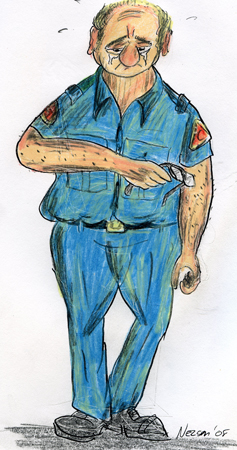
\includegraphics[height=60mm]{corps/chapitre15/img/personnage-timothee-pleur.jpg}
\end{floatingfigure}

L’improbable aveu a pour effet de pénétrer l’armature de Timothée qui, pour la deuxième fois de la journée, se retrouve entièrement déstabilisé et incapable de se contenir. Malgré une idée furtive indiquant qu’il torpillait toute chance, pour peu qu’il en eût, auprès de la belle infirmière, il se brise en sanglots.

- T’es bien chanceuse de le savoir, sanglote-t-il, moi, je ne l’ai jamais su. Va-t-y falloir que j’attende d’avoir 82 ans ?

Les mains sur la monture de ses verres, il part se réfugier dans la cuisine où, instantanément, Romain va l’enserrer dans ses bras. Gazou émet un début de grondement, mais il replace ses yeux sur Béatrice et reprend sa contemplation. C’est la vieille qui casse la glace, initiative qu’apprécie la visiteuse qui lutte elle-même pour ne pas chavirer dans les eaux de ses émotions.

- Ch’est vrai que je ne lui ai jamais dit que je l’aimais, pauvre p’tit garchon. Pourtant, pourtant …

Elle ne finit pas sa phrase.

- Maudite vie, reprend-elle. J’ai eu une vie complètement foquée.

Deuxième miracle de la soirée, Marie, fille de Marceline et d’Edmond Rioux, se met à se raconter, sans pudeur, sans le souci d’embarrasser cette étrangère qui semble si réceptive. Les mots vont sortir drus, puissants, libérés, comme une rivière longtemps empêtrée par un barrage de castor, ce qui lui a donné l’allure d’un petit lac, et qui, soudain, se met à couler et à couler. Pour la première fois de sa vie, la Maririou déballe son histoire. Elle se l’offre à elle, sans fixer personne, ni Romain ni Timothée qui se sont approchés, ni Béatrice dont les yeux sont humides. Elle regarde le tapis et, à grands coups d’archet, achève la destruction de sa maison de castor.

Au même moment sur la rue Crouet, une voiture est immobilisée en face du cimetière. Marie-Odile qui n’avait plus de Midol pour calmer ses douleurs était sortie s’en procurer à la pharmacie. À son retour, elle avait décidé de venir se «racheter» auprès de Timothée, convaincue que plus tôt dans la journée, elle n’avait pas été à la hauteur de l’accablement avec lequel il était aux prises. En débouchant sur la rue, elle a aperçu une voiture stationnée devant la maison de son amant, phénomène inhabituel puisqu’il déplorait ne jamais recevoir de visiteurs, et, en femme flic, bien que lourdement menstruée, elle a voulu savoir qui en était le propriétaire. Utilisant sa boucle d’oreille et certaines habiletés policières, elle a fait une courte recherche et a pu apprendre que la bagnole était au nom d’une certaine Béatrice Martin.

C’est ce véhicule qu’elle regarde présentement, la mâchoire crispée et les yeux en tempête.
\chapitre{Sanglots sur une vie brisée, le 27 juillet 2033 }{Tout ce qu’on fait dans la vie, même l’amour,}{ on le fait dans le train express qui roule vers la mort», avait écrit en 1928 l’artiste controversé Jean Cocteau lors d’une cure de désintoxication. Puisqu’il fumait de l’opium pour pouvoir «quitter le train en marche» et s’occuper d’autre chose que de la vie et de la mort, il n’avait pas encore réalisé qu’avec les années, le train devenait fou de vitesse, ivre de regret et prisonnier de ses rails, qu’il devenait de plus en plus infernal, fonçant dans un «voyage au bout de la nuit», celui de l’absurdité et de la pourriture dépeintes quelques années plus tard par Louis-Ferdinand Céline. Inexorablement, kilomètre par kilomètre, keclic-keclac, keclic-keclac, keclic-keclac, l’éclairage disparaissait, ce qui amenait le passager, de plus en plus apeuré, à vouloir mettre sa vie en lumière, comme pour se rassurer, à donner un sens à son errance, comme s’il eut fallu qu’il y en est un.  }

Et il s’y acharnait avant que la loco, celle de High Noon, le film culte de Fred Zinnemann, en vienne à siffler ses trois dernières prises, celles d’un arrêt sans buffet, sans gare, sans soleil, sans rien, le laissant abandonné, trahi, oublié, devant les forces obscures. «Trois prises ! Reeeetiréééé !» 

La Maririou qui ne dispose ni du surréalisme multidisciplinaire de Cocteau, ni de l’anarchisme cynique de Céline, ni de l’antimaccarthysme romantique de Zinnemann, vient de débarquer du train, attirée comme un papillon nocturne par une soudaine lueur dans le noir de la lumière disparue, lueur aussi blafarde que merveilleuse d’une allumette tenue à bout de bras par Marceline des Bezo. En râlotant, soufflant, chuintant, elle s’active devant Béatrice, Romain et Timothée, tous trois mis en sentiment par la chanson thème «Et toi aussi tu m’abandonnes», à déboulonner avec une clé à molette aussi longue que son archet, le sens qu’avait sa vie, celui dont l’épicentre était régi par les conventions musicales. Non pas pour redonner un sens au parcours accompli, tout le monde s’en fiche, y compris elle, mais plutôt pour aller, de ses pas précipités de petite vieille armée d’un parapluie, prendre le contrôle de la locomotive et donner cours à cette urgence de dire ce qui aurait dû l’être bien des années avant. Cocteau, Céline et Zinnemann n’avaient pu imaginer en leur époque qu’un jour, il y aurait la mentalité baby-boomer.

D’un ton sans appel, d’une voix définitive, elle raconte avoir passé sa vie à prétendre être musicienne violoncelliste, alors qu’elle ne l’était pas. Elle déclare n’avoir fait que besogner, gratter, peiner, triturer, sept jours sur sept, par temps de soleil, de grippe, de vide, pour en arriver à devenir une «bonne technicienne en manipulation de violoncelle». Eut-elle été musicienne violoncelliste, eut-elle été artiste, elle aurait été à l’écoute de la sensibilité des autres. Il aurait été naturel pour elle de vouloir l’enrichir, la nuancer, la soutenir, la compléter. Elle aurait su comment, et à quelle dose, ajouter sa petite particularité à elle dans l’émotion collective d’un ensemble musical. Mais non, elle ne vivait que pour ces œuvres où le violoncelle semble prendre toute la place, ces pièces magnifiques de Fauré, ces sonates et autre Allegro appassionato de Saint-Saëns, de Debussy, de Chopin, de Mendelssohn ou de Schubert, ces concertos pour violoncelle de Dvořák, de Boccherini, de Beethoven ou de Brahms. Et quand elle pouvait attirer tous les éclairages sur elle, quitte à laisser ses camarades dans le noir, elle le faisait du mieux qu’elle le pouvait. Ainsi, sous son archet, les deux concertos pour violoncelle de Chostakovitch devenaient des joyaux de perfection technique donnant droit aux vivats de la salle. Hélas!, insiste la Maririou, ce n’était que l’expression d’une habileté particulière, la prestation égotique d’une prouesse sans âme.

- Mon âme était rechtée dans le coffre d’une Impala rouge.

Incapable de remettre les pieds dans l’univers Bezo après le drame, Marie est allée vivre chez la cousine Lise à Rimouski, puis chez sa tante Denise à Québec; une petite boulotte toute gentille et sans enfants. Fortement repliée sur elle-même, parlant à peine à la sœur cadette de sa mère et presque jamais à son oncle Robert, un bon diable de plombier ronchonneur, la gamine s’est vite isolée dans sa chambre, on aurait dit une sauvageonne qui n’avait pas appris à sourire. Elle s’est raccrochée à la musique avec le gros crincrin du cousin Lucien, un «prêt à très long terme, ma chouette», et a choisi de ne pas fréquenter d’amis. De toute façon, elle n’en avait jamais eus.

Étonné par ses progrès plus que rapides à l’instrument, le couple de braves gens se met en tête d’inscrire la petite à des cours privés. C’est ainsi qu’un soir après souper, Denise l’amène dans le quartier Saint-Jean-Baptiste chez Michaela Prochazka, une violoncelliste tchécoslovaque qui s’était expatriée en 1945 juste avant que ne se referme l’étau soviétique. Entre 1938 à 1945, la dame avait joué avec l’Orchestre philharmonique tchèque, une formation très réputée qu’avaient naguère dirigée Antonín Dvořák, Gustav Mahler et Václav Talich.

- J’me chouviens des photos qu’elle m’a montrées. Tout était vrai; elle n’avait rien inventé. Mon Dieu que j’étais imprechionnée. Imaginez : être dirigée par Václav Talich !

À 82 ans, Marie se rappelle sans hésitation des noms de Michaela Prochazka et de Václav Talich. Elle n’a pas oublié, non plus, le fils de Mme Prochazka, ce petit salopard de Lukas. Elle revoit le salon de ce rez-de-chaussée, rue d’Aiguillon. Elle se remémore parfaitement bien le jour où sa professeure lui avait permis d’essayer son merveilleux instrument, une vénérable antiquité achetée à Belgrade dans les années 20.

- Je pense que chette femme m’a aimée.

Aimée, il faut le croire, puisque Robert Bérubé, qui s’était mis à son compte deux ans plus tôt, fait faillite en 1967. Le couple doit déménager dans un logement de Saint-François-d’Assise et se retrouve en situation de ne plus pouvoir supporter les cours privés. Heureusement pour la gamine, il n’est pas question de la retourner chez sa mère dans le Bas-du-Fleuve. «Y a des maudites limites à la misére», affirme Robert, l’œil humide. Apprenant la nouvelle, Mme Prochazka offre sans aucune hésitation, un peu comme si elle choisissait une partition, de continuer à enseigner gracieusement, ce qu’elle fera avec le plus grand sérieux jusqu’à l’admission de Marie au Conservatoire de musique de Québec.

- À chette époque, mon oncle Robert dijait que les doigts de ma main gauche étaient tellement forts que les jommes avaient peur de moi. T’as jamais eu peur que j’te torde le cou, Romain ?

- Non parce que j’ai toujours eu le cou plus gros que ta main. Mais ta langue, par exemple, ouf !

Sa formation a eu comme cadre unique la ville de Québec où tout se termine en 1972 avec un Premier Prix du Conservatoire de musique de Québec en violoncelle, ce qui lui permet de faire quelques remplacements à l’Orchestre symphonique de Québec et à la Société de musique contemporaine du Québec. Mais, ambitieuse insatiable, elle veut fréquenter la célèbre Juilliard School de New York, une perspective nettement au-dessus de ses moyens. D’où la France, pays avec plein de gens cultivés où, assurément, il est possible de gagner sa vie avec un violoncelle, là-bas, et même de se ramasser un pactole, ce qui contribuera à se payer la Juilliard. Une semaine après être débarquée, elle signe un contrat avec l’Orchestre philharmonique Rhône-Alpes à Lyon, emploi qu’elle s’était déniché directement de Québec, ce qui lui permet de s’acheter un instrument fabriqué à Mirecourt au début du XXe siècle. 

\begin{floatingfigure}[l]{45mm}
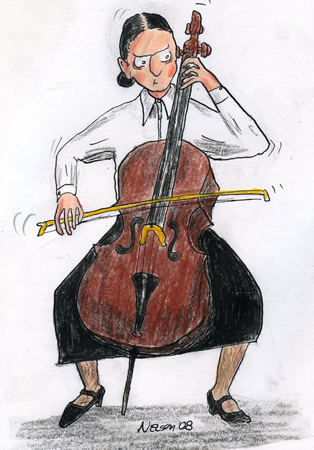
\includegraphics[height=60mm]{corps/chapitre16/img/personnage-marie-musique.jpg}
\end{floatingfigure}

Pendant huit ans, elle arpente ainsi les coins et recoins de l’Hexagone et, à bien y penser, en déborde à plusieurs reprises. Par contre, elle doit faire son deuil des grands orchestres symphoniques, ceux de Berlin, de Munich, de Londres. Quand elle tente sa chance auprès de l’Orchestre symphonique de Navarre Pablo Sarasate, l’humiliation qu’elle en ressent lui sert une leçon qu’elle méditera toute sa vie : connaître sa force, savoir quelle est sa place et ne jamais «péter plus haut qu’le trou !»

Pendant huit ans, Marie Rioux se tire d’affaire avec d’excellentes formations, quoique de moindres envergures, tels l’Orchestre symphonique de Tours, l’Orchestre Symphonique Municipal de la Ville de Nice ou l’Orchestre du Capitole de Toulouse et elle a collaboré avec de très jeunes ensembles dont l’Orchestre national de Lille ou L’Orchestre national d’Île de France. Elle travaille également avec de plus petits groupes, dont à Bernes et à Genève avec un quatuor à cordes, à Marseille et à Lyon avec un orchestre de chambre. Mais surtout elle tyrannise pendant deux ans, la douzaine de valeureux musiciens de l’Orchestre de Chambre de Toulouse. C’est que partout, la «fille à Marceline» se retrouve en situation de coups et blessures. On la déteste uniformément : violoniste qui se fait détruire sa tenue de concert, une autre qui découvre ses partitions dans une cuvette souillée, violoncelliste concurrente à qui elle cache une importante pratique, altercation en plein récital dans un musée bernois, volée d’injures en français bas-laurentien envoyée à un maestro de son âge, un Danois qu’elle jugeait obnubilé par son ego, et ainsi de suite.

1 mètre 80, svelte, élégante, normalement vêtue de noir, le port altier, le visage très beau bien que fermé, les yeux de la couleur du fleuve lors des grandes marées d’automne quand il arrache tout son fond pour en faire une bouillie qu’il recrache sur ses berges, Marie subit régulièrement des tentatives masculines de rapprochement, des manœuvres libidineuses à peine masquées, des passes grossières de drague, voire quelques propositions directes qu’elle reçoit comme des soufflets. Elle arrive toujours à tout repousser. Même Arnaud Muller, virtuose de la flûte traversière, qui l’aime à en vouloir mourir. Il est prêt à tout abandonner pour elle, dont sa femme et sa fillette. Quand la violoncelliste apprend ce détail en dînant dans un quatre fourchettes de Grenoble, elle fait un tel esclandre, incluant son Côte du Rhône dont elle asperge la figure du malheureux, que l’amoureux éconduit quitte l’orchestre, défait, découragé, misérable.

Côté disque, elle n’en aura jamais un à son nom, contrairement à ce que colportera, par après, la rumeur culturelle de la région rimouskoise. Par contre, en tant que musicienne dans une formation, elle va participer à plusieurs reprises à des enregistrements, des initiatives qui la laisseront de glace, mais qui la frustreront à l’occasion, surtout quand elle ne pourra s’agiter les crins que sur quelques portées. Ce que l’on grave, déplorera-t-elle, semble toujours être conçu pour mettre n’importe quel instrument en valeur, sauf le violoncelle.

Tant et si bien qu’à la fin de l’hiver de 1980 Marie Rioux, à la veille d’avoir 29 ans, est devenue une boule de nerfs prête à exploser. Vierge, solitaire, isolée, crainte, détestée, désillusionnée, mauvaise, crevée morte, elle va consulter un médecin toulousain qui lui colle un diagnostic de surmenage professionnel, ce syndrome d’épuisement dont la médecine faisait alors de plus en plus de cas.

- Il faut arrêter quelque temps, ma p’tite dame. Sinon, crac, ça sera la camisole !

- Me semble qu’avec un p’tit remontant, je passerais à travers, non ?

- Plaît-il ?

- Z’avez pas des pilules qui me tireraient d’affaire ?

- Je vous parle de votre vie et vous me causez de «pilules». Soyez sérieuse, il vous faut vous soigner.

- Me soigner …

- Vous reposer, ma p’tite dame, seulement vous reposer, sans rien faire d’autre. Je veux bien vous prescrire des cachets, mais seul le repos pourra vous amener à un complet rétablissement.

La jeune femme repart avec, en poche, une prescription appréciable et la justification médicale d’un arrêt de travail. Comme elle est sur le point de partir en tournée avec l’Orchestre de Chambre de Toulouse, aussi bien en Espagne, au Canada, qu’aux É.-U., elle s’entend pour être remplacée le plus tôt possible et, coïncidence, le nouveau violoncelliste est attendu après la prestation de Québec, la quatrième au Canada.

C’est un concert de musique baroque, essentiellement du Mozart, qui, en ce beau dimanche après-midi de printemps, a pour cadre le Musée de Québec, sur les Plaines d’Abraham. Tout au long, Marie y bouge son archet comme si elle était zombie. Ce qu’a bien sûr remarqué Rhéa Théberge, l’institutrice du 2e Rang Ouest de Saint-Fabien, qui est assise dans la salle, son programme utilisé comme éventail. Le récital terminé, elle s’approche de la pièce où sont passés les musiciens et demande qu’on avertisse Marie Rioux de sa présence.

- Tu n’as presque pas changé depuis la dernière fois que je t’ai vue; c’était à Rimouski. Tu es seulement plus grande et plus jolie.

Marie reconnaît cette femme qui l’a initiée à la lecture, à la musique, à la connaissance, cette femme qui a catalysé sa sortie d’un milieu malsain.

- Mamzelle Théberge ?

- Oui ma belle, c’est moi, de répondre l’enseignante devenue quadragénaire avancée, en embrassant généreusement son ancienne pupille.

Cernée, les traits tirés, amaigrie, la musicienne explique sa situation. C’est son dernier concert; on l’a mise au repos et elle en a au moins jusqu’à l’automne, si ce n’est plus. Après ? Elle ne le sait trop. Peut-être rappliquera-t-elle en France reprendre le collier. Elle est sous contrat avec l’Orchestre de Chambre de Toulouse, une chic organisation dont elle ne veut surtout pas abuser; elle leur en a assez fait subir. Elle est aussi en sabbatique avec l’Orchestre du Capitole de Toulouse, mais n’a vraiment pas envie d’y retourner. Peut-être ira-t-elle plutôt étudier à New York. Pour l’instant, elle est sous l’effet des médicaments et ne veut plus penser à rien. Non elle n’a pas de mari ou d’ami de cœur et cela est bien loin de ses préoccupations. En fait, elle n’a ni chat, ni chien, ni canari, ni plante, ni maison. Elle n’a qu’un petit studio qu’on ne lui loue pas cher, rue de Mirepoix, un «chouette quartier à deux pas de la Garonne».

- T’es quasiment rendue avec un accent français ?

- Ça se corrige !

- La Garonne, chanceuse !

Marie frise le début de sourire.

- Ouais. La Garonne, c’n’est peut-être pas un vrai bras de mer, un vrai fleuve salé comme le nôtre, mais c’est un cours d’eau qui a son charme.

À son tour, Rhéa raconte qu’elle a abandonné sa petite école depuis belle lurette; en fait, il n’en existe plus d’écoles de rang. Les citadins les ont achetées. Ils en ont fait des maisons, des chalets. Non, depuis quelques années, elle s’occupe passionnément de jeunes en difficulté, de cas complexes issus de familles dysfonctionnelles, monoparentales, miséreuses, de victimes de violence, des enfants parfois traumatisés pour le restant de leurs jours. Tous souffrent d’un énorme problème d’image, d’absence de perspective leur permettant de voir qu’ils pourraient peut-être s’en tirer. Et en les parquant dans une même école, dans une même classe, la commission scolaire les a ghettoïsés. Autour d’eux, ils ne voient que malheur, échec, pauvreté et médiocrité. Sans compter qu’ils sont discriminés et ridiculisés par toutes les autres classes.

- Mais toi, Marie, tu représentes tout le contraire. Tu t’en es sortie. En dix-huit ans, tu es passée de la misère noire du 3e Rang Ouest à un studio près de la Garonne. Tu voyages, tu donnes des concerts et tu gagnes très bien ta vie. Et en Europe par-dessus le marché ! Et si je me fie à ce qui est en vente à la sortie de la salle ici, tu joues dans des 33 tours. Ça, moi, j’appelle ça réussir sa vie de façon extraordinaire.

La jeune femme commence à vouloir filer; elle perçoit très bien où cette conversation s’en va.

- Je vais être bien honnête avec toi. Je suis venue pour te demander une faveur.

- Vous voulez que j’aille rencontrer vos enfants, que je leur prouve qu’on peut s’en sortir, que dans le fond, un père qui nous bat, une mère qui nous boit des verres de gin sous le nez, c’est grave, mais que le fait de cesser de rêver qu’on va s’en sortir, l’est encore plus ? C’est ça ?

- À peu près ça, oui.

- Oubliez ça, mamzelle Théberge, j’en suis incapable. J’ai de la misère à vivoter dans mon petit monde à moi, un petit monde gros comme ça dans ma pauvre caboche. J’ne commencerai pas à aller le présenter à d’autres en le quittant temporairement pour pouvoir entrer dans le leur. J’n’en suis pas capable. Vraiment pas. Il est faux de croire, mamzelle Théberge, que je m’en suis sortie ! À force de ne pas savoir comment inventer la machine à remonter le temps qui me permettrait d’aller rescénariser mon enfance, je suis devenue une garce invivable que tout le monde déteste. Et faut absolument que je me repose !

C’est à ce moment que la quémandeuse sort l’arme-choc de sa besace. Hypocritement, elle lui parle d’une petite fille de 11 ans, sa copie carbone, 18 ans en arrière, une enfant perdue, recluse, fermée, incapable de sourire, jamais d’amis, battue et laissée pour compte par une monoparentale toxicomane de Rimouski-Est. La totale !

Dans la tête de Marie, deux fils oubliés viennent se toucher et toute son expression change. La perfide Rhéa a gagné !

Quelques jours plus tard, la musicienne est debout devant une classe en apparence normale. On a beau voir à leurs vêtements que les deux douzaines d’enfants sagement assis ne sont pas riches, rien n’indique qu’ils sont des pestiférés normatifs. Si certains semblent enchantés de rencontrer cette co-miséreuse d’une autre époque, la plupart l’écoutent avec de grands yeux gênés. Mais tout au fond, physiquement en retrait, une petite fille, probablement de onze ans, fait semblant, du mieux qu’elle le peut, de ne pas l’entendre ni la regarder.

- Comment t’appelles-tu ? lui demande Marie.

- A parle pas, madame, crie un gamin. Elle s’appelle Sonia Gagné.

Dès lors, la jeune femme n’a d’yeux que pour cette fillette. Elle ne semble plus parler qu’à elle. Même que le soir, invitée à coucher chez Rhéa, une sorte de commémoration des occasions où il ne faisait pas beau dans le rang, elle questionne abondamment son hôte sur la petite Sonia. Elle veut tout savoir. On la dirait fascinée. Dans sa tête, une mission surgit : sauver cette enfant. Elle doit le faire. Ce n’est pas pour rien que le destin les a mises en présence, toutes les deux.

Le lendemain matin, avant de s’en retourner au terminus d’autobus, elle demande au chauffeur de taxi de l’amener à un magasin de musique où elle achète un harmonica. De là, elle passe à l’école, donne le petit instrument au secrétariat afin qu’on le remette, de sa part, à Sonia Gagné et file vers son car.

- Là, cha va aller vite, continue La Maririou. Ma tante Denije à Québec avait un cougin qui louait des chalets au lac Chaint-Mathieu. Le mois chuivant, je l’ai appelé et il m’a organigé quek’chose de pas pire, achez proche du lac et achez loin des gens.

Pendant les deux dernières semaines de juin, la convalescente séjourne au lac où elle se divertit à chasser les écureuils, les ratons laveurs et les oiseaux qui viennent les importuner, elle et son violoncelle, dans les innombrables pièces de ce château qu’elle a tôt fait de se construire dans son monde imaginaire, un monde salutaire qu’elle avait toujours eu le loisir de rendre totalement étanche aux réalités qui, ça et là, l’agressaient. Une irrépressible impulsion l’amène cependant à prendre régulièrement des nouvelles de la petite Sonia. Oui elle s’amuse avec son harmonica. Non elle ne s’est pas informée sur sa bienfaitrice. Oui elle a terminé ses classes. Non elle ne sera pas promue au degré supérieur.

L’avant-veille de son départ pour Québec, elle apprend de Rhéa la création de l’École populaire de Musique, un projet communautaire du milieu où il est question d’initier des enfants et des adultes défavorisés aux joies de la musique par l’apprentissage d’un instrument. Elle a pris sur elle d’y inscrire Sonia en violon…

- T’as dix-huit ans de violoncelle dans le corps, ma belle, tu dois bien savoir jouer du violon, non ?

C’était en effet un instrument que Marie maniait avec une certaine dextérité, mais une dextérité ampoulée, rigide, classique et fort peu violoneuse.

- J’te dis ça d’même parce qu’il y a eu trop d’inscriptions en violon; ils manquent de profs.

Comme elle tourne en rond, qu’elle ne sait trop quoi faire de ses 10 doigts, qu’elle n’a vraiment pas envie de s’installer chez sa tante Denise, qu’elle a suffisamment d’épargne pour se permettre de ne pas travailler pour presque un an, qu’il pourrait être judicieux de se changer un peu les idées et que, dans le fond, elle pourrait aider la petite Sonia à s’en sortir, la jeune femme demande à l’enseignante de venir la chercher. Elle rencontrera les autorités du projet.

Le responsable de l’enseignement, Pierre Dugrain, est un professeur de violon au conservatoire local qui se met à saliver devant le CV que la violoncelliste lui dépose sur la table du bar où il la reçoit sans cérémonie.

- Premier prix en violoncelle, Orchestre Symphonique de Tours, Orchestre Symphonique de Nice, Orchestre du Capitole de Toulouse, Orchestre national de Lille, Orchestre national d’Île de France, Orchestre de Chambre de Toulouse, barnak, t’en a fait du millage ! Maudit beau CV !

Marie se fait prudente.

- Je suis violoncelliste, pas violoniste.

- Barnak, c’t’une job de bénévole qu’on t’offre. On rentrera pas la Guilde des musiciens dans notre affaire, casse-toi pas la tête ! Par contre, continue Dugrain, je sais qu’au Conservatoire, on a besoin d’un chargé de cours en violoncelle pour septembre. Si ça t’intéresse, va appliquer. Avec un CV comme le tien, t’es certaine d’avoir la job. Pis là, b’en c’est pas du travail bénévole. Tu veux une bière ?

- Merci, j’bois jamais d’alcool, qu’elle répond avec douleur, revoyant les caisses honnies que son père vidait à l’époque.

Ici, raconte la mère de Timothée, il y a tout un paradoxe à expliquer. D’une part, elle devient très rapidement «la Maririou», un personnage austère, exigeant, autoritaire que collègues et étudiants adorent détester. Ainsi, dès le départ, elle fait croisade contre le fait que la gestion d’un si beau projet avait été confiée à une clique de noceurs, incluant Dugrain, qui tenaient l’essentiel de leurs réunions décisionnelles dans une buvette aussi malfamée qu’enfumée du centre-ville de Rimouski. Pour elle, une telle pratique était illégale, inefficace et non respectueuse auprès des membres de l’équipe qui ne fumaient pas, ne prenaient pas de drogue et ne consommaient pas d’alcool, dont elle était probablement la seule représentante. Elle en fait tant, qu’elle se retrouve isolée et tournée en dérision. Marie se replie donc, coupe tout contact non essentiel et demande à ce qu’on ne lui affecte plus que des moins de douze ans, les plus mal en point, insiste-t-elle, ce qui, bien sûr, inclut Sonia Gagné. Encore là, sa nature conflictuelle prend le dessus. Des enfants se plaignent, d’autres se présentent de plus en plus rarement. Seuls les plus timides semblent se résigner à continuer. Quant à Sonia, elle finit par réagir en abandonnant définitivement ses cours. Elle conserve toutefois l’harmonica.

- Je l’ai jamais revu ch’te pauvre p’tite fille-là. Chi elle est encore vivante, elle doit bien avoir proche 65 ans. Timothée est à veille d’la voir entrer au Chentre !

D’autre part, elle subit humiliation sur humiliation, accepte le sobriquet de Maririou, continue de donner toutes les heures qu’on lui demande, essaie par tous les moyens de mettre de l’eau dans son vin pour que les petits démunis qu’on lui envoie ne souffrent pas trop. Elle devient la personne la plus fiable de l’École et même Dugrain est obligé de le reconnaître, lui qui doit, par ailleurs, s’immiscer dans une jacquerie d’étudiants du Conservatoire incapables de supporter l’extrême rigueur de la chargée de cours. Malgré tout, elle demeure fidèle à ses engagements de l’été 80. Jamais elle ne fléchira. On dira d’elle qu’elle est «le roc sur lequel l’École a été bâtie». En fait, elle négociera avec les édiles de son village pour que de façon nominale, l’École puisse louer une ancienne maison bourgeoise saisie pour taxes non payées. Grâce à une armée de bénévoles et de donateurs, le bâtiment sera rénové et adapté aux besoins de l’enseignement musical, cela sous la supervision constante et méticuleuse de la Maririou.

- Mais j’ai fini par m’adouchir avec le temps, dijons que je me chuis calmée. Je pense que ch’est Romain qui a eu le dechus. 

\begin{floatingfigure}[l]{40mm}
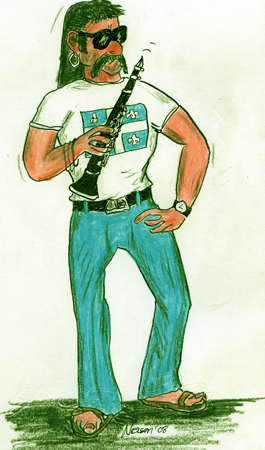
\includegraphics[height=60mm]{corps/chapitre16/img/personnage-romain-jeune.jpg}
\end{floatingfigure}

Romain, le beau clarinettiste autodidacte qui lui a vraiment fait basculer sa vie ! Il lui a essentiellement démontré qu’elle ne comprenait rien à la musique. Pour elle, c’était un travail douloureux qu’il lui fallait accomplir à la perfection, une peine quotidienne, constante, truffée d’exigences pas possibles, un délire exutoire que l’on devait présenter à des gens ayant payé et devant applaudir. C’était accepter des conditions scandaleuses pour plaire à de rondouillets bourgeois ravis, repus, roteux. C’était consacrer sa vie à se battre entre collègues pour une petite place dans un ensemble que viendra peut-être entendre le politicien, le financier, le m’as-tu-vu, des salauds sans sensibilité artistique qui auront une influence sur la survie financière de la formation musicale. C’était traîner son étui à violoncelle d’orchestre en orchestre pour appuyer la tendance voulant que la musique soit une business faisant surtout vivre des gens, analphabètes devant une partition, mais très habiles en marketing et en relations publiques. Or, a répété Romain autant de fois qu’il l’a pu, la musique ne peut être qu’un plaisir constant, qu’une joie solitaire pouvant évoluer en trip entre copains, en concerts gratuits dans des endroits sympathiques, en jam-sessions entre instrumentistes et autres tapeurs de pieds.

- La musique, on la fait pour soi, pour se faire plaisir, pour se faire du bien. On joue de la musique. On apprend aux autres à jouer, pas à suer !

Toute une conception, tout un projet de société ! Quoi qu’il en soit, le gaillard lui a fait découvrir une planète qu’elle ignorait. Partie toute jeune d’un environnement miséreux, elle a vécu chez des gens modestes de Québec, puis s’est acclimatée au sud de la France sans fréquenter personne. La voici maintenant dans un monde de marginaux qui s’aménagent d’impressionnants jardins engraissés au capelan, qui s’essaient dans l’élevage de petites chèvres, de lapins et de volaille, qui produisent des variétés touchantes de confitures, de gelées, de ketchup, de conserves, qui confectionnent eux-mêmes leurs rideaux, leurs carpettes, leurs couvre-lits, qui n’ont jamais moins de cinq chats et deux chiens, des énormes, qui conduisent des camionnettes rafistolées et qui, avec respect, s’établissent dans des villages traditionnels. Un univers de filles en robes longues, bottées comme pour faire le train, sans jamais de soutien-gorge et qui se roulent leurs cigarettes, de gars qui ne se taillent plus la barbe, qui ne portent que des bottes «capées», qui achètent leur Dow en caisse de 24 petites ou de 12 grosses et qui se disent en accord avec les revendications féministes.

Eux, Marie et Romain, ils s’installent au sortir de Saint-Anaclet, sur les hauteurs de Rimouski, dans une maison épouvantablement maganée dont le terrain d’une dizaine d’acres pourrait devenir intéressant. Or, contre toute probabilité, ils vont y demeurer 47 ans. Grâce à Romain, la jeune femme apprend à vraiment sentir une fleur, à bien observer un bourdon, à mâchouiller et déguster un brin de foin, à jouer avec une portée de chats, à batifoler nue dans certaines anses du Bic, à fréquenter les gens sans leur arracher les yeux, à boire des grosses bières, à ne pas se laver tous les jours et surtout, à jardiner. Marie se découvre en effet le pouce vert.

Dès l’automne, elle sait qu’elle ne regagnera pas l’Europe. Là-bas, personne ne la manque et aucun ensemble ne lui fait parvenir d’offre d’emploi. C’est aussi à ce moment qu’elle devient convaincue que sa sexualité est «foquée». Elle ne peut commettre l’acte que gelée. Alors, elle peut ressentir un certain plaisir et parfois, du désir. Autrement, rien n’est plus désagréable, voire irritant. Faut-il préciser qu’elle ne met pas grand temps à adopter la béatitude des drogues douces, ce qui l’amène à connaître l’essentiel état de détente qui lui avait fait défaut jusque-là. Quant à son mauvais garçon d’amoureux, il s’ouvre à la discipline des partitions musicales, ce qui lui permet d’acquérir un peu de rigueur, qualité dont il était cruellement dépourvu.

Pendant les dix premières années, ils vivent d’expédients, d’aventures, de trafics dérisoires et de miracles. Chaque année, la Maririou chasse son beau Romain et, à chaque fois, elle le regrette. Sur une base irrégulière, elle enseigne à des jeunes dans le cadre du projet et, contre rémunération, ses économies ayant été dissipées, à des étudiants du conservatoire. De temps en temps, il arrivera une petite fille de onze ans toute poquée que Marie essaiera d’initier à la musique. Parfois, ça semblera vouloir fonctionner pour quelque temps, parfois ça ne lèvera pas. C’est dire les frustrations de cette nouvelle Michaela Prochazka qui veut à tout prix aider ces victimes d’un émule d’Edmond Rioux.

Il en est ainsi jusqu’en 1990 quand, à 39 ans, elle donne naissance à Timothée-Milet. Tout change alors. Vraiment. Romain embrigade ses deux frères, des Longueuillois, dans une offensive majeure au terme de laquelle un banquier lui consent l’hypothèque nécessaire à l’achat de cette brinquebalante maison qu’ils louent depuis les débuts à Saint-Anaclet. Au printemps suivant, il accepte même ce travail de livreur en fourgonnette que lui propose un voisin, l’homme d’affaires Gilles Lévesque. Dès lors, il coupe radicalement dans sa consommation de hash et se résout, sans bougonner, à se taper toutes les heures supplémentaires qu’on lui impose. C’est ce cabotage routier qu’il fera sur les routes locales et régionales pendant les trente prochaines années, sans jamais déplaire. De son côté, Marie ramasse tous les cours qu’on lui confie et se met à produire des confitures, des conserves et des fines herbes qu’elle vend dans un petit stand que lui aménage Romain près du chemin devant leur maison.

- À partir de là, cha va être la routine et le temps va filer.

Romain veut nuancer.

- T’oublies le lac Saint-Mathieu. On y a loué une roulotte à tous les étés …

- On l’a fait entre 1997 et 2015, deux chemaines par été.

Le lac Saint-Mathieu, ce sera leurs vacances annuelles. Marie réussira à combiner ce court séjour avec un mini camp musical où certains enfants seront conviés aux frais de l’École. Sans s’occuper de cette marmaille dans le quotidien, elle supervisera individuellement leur pratique instrumentale. Eh oui, Timothée, il y a eu la petite Julie, cette nièce catégorie fesse gauche de Luce Morency, une fillette qui lui semblait vraiment intéressée à se donner à la musique, à fuir son univers sordide, une petite fille très sensible qu’en cet été 2001, elle a rapidement aimée et placée au centre de ses préoccupations quotidiennes.

- On l’a retrouvée battue à mort en janvier 2010. Elle était gelée comme une crotte, plantée dans un banc de neige comme un piquet à côté du prechbytère d’Amqui. On n’a jamais chu ch’qui ch’était passé. Cha m’a fait de la peine, pauv’ ‘tite fille !

À deux occasions, la Maririou va s’impliquer en politique, une fois localement, une autre, au niveau du comté. En 2014, des édiles municipaux veulent mettre la main sur la bâtisse louée un dollar par année à l’École de Musique quinze ans plus tôt. Ils ont beau jeu, la paperasse semble avoir été un peu bâclée à l’époque. Leur projet ? Raser l’équipement et récupérer le terrain pour agrandir le mini mail voisin. La perspective étant jugée inacceptable, Marie s’en va-t’en-guerre, fait du porte-à-porte et se fait élire conseillère. C’est ainsi qu’elle va arriver à tout bloquer. À la table du Conseil, elle va devenir une mère chat à qui de méchants roquets de perron veulent enlever ses chatons. La bataille sera terrible et, au terme, les promoteurs devront baisser pavillon ayant épuisé toutes leurs ressources et leur patience. Presque vingt ans plus tard, on en parle encore.

En 2019, un courant de pensée visant à sabrer les dépenses culturelles sévit, encore une fois, à la grandeur du Québec. Ainsi, la survie de l’École est en jeu. À 68 ans, Marie va aller cogner chez Sylvain Turcotte, un fils de cultivateur qui a été désigné comme nouveau candidat libéral pour le comté de Rimouski. Méticuleusement, comme s’il s’agissait de l’enjeu politique le plus important de la planète, elle lui expose toute la problématique et le convainc d’intégrer la survie de l’École dans sa plate-forme électorale. En contrepartie, elle accepte de l’appuyer publiquement, elle la grande musicienne qui a endisqué, qui a joué partout, cette vedette internationale qui a amassé tous les prix et qui est respectée par tous les chefs d’orchestre au monde. En outre, elle décide de travailler lourdement à son élection. Il est important de souligner que cette fois, la Maririou n’est pas, comme à son habitude, le pire des fléaux. De nombreux bénévoles libéraux attribuent cette dignité à Mimi Turcotte, directrice adjointe de l’organisation libérale pour le comté de Rimouski et mère du candidat. Il va de soi que Marie se découvre ici un alter ego, une femme aussi tête de nœud qu’elle-même pouvait l’être. On connaît la suite, le gros Turcotte, élu haut la main grâce à un taux de participation de plus de 45 %, sera nommé ministre et, malgré ses promesses maintes fois répétées de soutenir l’École envers et contre tous, il ne lèvera pas son auriculaire boudiné pour la protéger quand, deux ans plus tard, elle devra fermer définitivement ses portes faute de pouvoir se financer adéquatement. C’est une disparition qui affectera profondément Marie; il n’y aura plus jamais de petites filles de 11 ans à tenter de sortir de la misère.

Lorsqu’en 2021, Romain va décider qu’il en a assez et qu’il prend sa retraite – il est âgé de 70 ans - la vie du couple va, dès lors, devenir plus difficile. Les piges au conservatoire seront de plus en plus rares et le jardin de plus en plus ténu.

- Ch’est pour cha que j’ai tellement pouché fort pour que tu acchepte le contrat sur la Côte-Nord avec Jérôme Dubé.

Romain se garde bien de répondre. Il lorgne plutôt Gazou qui dort, son horrible tête dans ses petites pattes crochues. Marie boit une gorgée d’eau avant de conclure.

- Cha été cha, ma vie !

Une vie où, insiste-t-elle, elle est passée à côté de l’essentiel, non pas sa carrière musicale, mais la vraie vie. Elle a vécu 70 ans convaincue que sa mère ne l’avait pas aimée, qu’elle ne l’avait pas défendue, qu’elle avait tué Edmond, ce père monstrueux, pour se défendre, elle, bien après que son enfant eut été battue sans qu’elle ne lève le petit doigt. Par la suite, Marie a passé sa vie à craindre les hommes, particulièrement ceux qui avaient de grosses paluches, «pas de belles mains de clarinettichte comme Romain», ceux qui parlaient fort, ceux qui voulaient décider pour les autres, ceux qui donnaient des ordres, «pas évident quand tu joues dans un orchechtre de chambre», ceux qui buvaient beaucoup.

Elle a imposé à son seul enfant et à son vieux compagnon des choix de vie qui ne leur convenait pas. Timothée, ce petit garçon rêveur, tendre, sensible, le cœur sur la main, elle l’a enfermé dans un enfer de musique-labeur, de respect de l’autorité, de crainte des femmes et de discipline incessante, cela par crainte qu’il ne ressemble à son grand-père Rioux, alors qu’il n’en avait pas du tout le caractère, contrairement à elle, Marie, qui en avait hérité quelques grands pans. Romain, ce vrai artiste, cette si bonne nature, cet homme de cœur et de vérité, elle l’a enferré dans une vie sérieuse, besogneuse, gratteuse, dangereuse et pire encore, alors que si elle l’avait laissé faire, leur vie aurait tellement été meilleure.

Elle cesse de contempler le tapis pour regarder son compagnon.

- Il y a 6 ans, je t’ai forcé à gâcher ce qui te restait de vie et par ricochet, chelle de Timothée ! Je m’en veux, tellement, tellement …

Elle a tenté d’aider de petites victimes à se sortir de leur misère en leur présentant une merveilleuse porte de sortie, mais aucune n’a voulu la suivre. Elle a cru que si la musique avait été la panacée dans son cas, il se pouvait qu’elle le soit dans leur cas. Mais était-ce bien une panacée ? Avec le recul, elle comprend maintenant – maintenant qu’il est trop tard - qu’elle n’a fait, à onze ans, que changer de cage et de système de valeurs. Elle sait aujourd’hui que la musique n’a jamais été une vocation, mais un refuge. Car, isolée dans le 3e Ouest de Saint-Fabien ou isolée dans sa musique, c’est, dans les deux cas, être coupée de la réalité. Comment, alors, peut-on faire en sorte que de petites filles toutes brisées en viennent à se raboudiner juste assez pour s’engager dans la vraie vie sur leurs deux pattes ?

- Je t’ai jamais remerchié, Romain, pour m’avoir montré che qu’étais la vraie réalité. J’aurais donc dû !

Un silence pesant succède au long récit. Timothée sait que s’il essaie de parler, rien ne sortira. N’a-t-il pas suffisamment étalé la preuve de sa désorganisation émotive ? Le vieillard, lui, a baissé la tête. Il vient de recevoir un premier remerciement en 53 ans de vie commune et ne sait trop quoi en faire. Sa réaction ne pourra qu’être brouillonne. Quant à Béatrice, elle arrive à bien mesurer toute l’intensité du moment et sent l’émotion lui agacer la luette.

C’est alors que pour la première fois depuis 1962, Marie Rioux, enfant battue de onze ans qui semble, cette fois, avoir abandonné la douce protection de son monde imaginaire, une cosmogonie complexe si loin de la vraie réalité, celle des petites filles qu’on retrouve mortes à Amqui dans un banc de neige, Marie Rioux descendue de son train sous les regards empathiques de ses proches, éclate en sanglots. C’est un pleur fait de hoquets lents, creux, typiques aux gens qui sans avoir désappris à pleurer, s’y remettent à l’étonnement général. Elle tente de se contrôler, de reprendre contenance, mais en vain. Elle essaie de parler, mais sa bouche ne lui obéit plus comme il le faudrait. Trop de peine doit en sortir.

- J’ai tout raté, parvient-elle quand même à exprimer, sans réaliser qu’à l’aide de son parapluie en canne, elle était en train de grimper dans une locomotive. Je vous demande même pas de me pardonner, il est trop tard pour cha. J’ai 82 ans et chuis enfermée dans un chous-chol.

La séquence est insoutenable. Alors que Romain et Timothée sont figés, Béatrice bouleversée par une telle expression de détresse, s’approche du fauteuil et se penche vers Marie pour l’enserrer dans ses bras. Doucement, elle lui caresse les cheveux.

Gazou que la scène a dérangé se rassure en apercevant la belle dame étreindre sa maîtresse. Il branle de la queue un instant et se replonge dans son sommeil.
\chapitre{Robespierre prend les commandes, le jeudi 28 juillet 2033 }{Vouloir atteindre le rêve d’une vie}{ ouvre parfois la porte à des raccourcis moraux pas toujours présentables dans les salons bienséants. Avec l’âge qui devient certain, il arrivera qu’on n’y regarde pas à deux fois avant d’avaliser une petite clause un peu particulière qui permettra néanmoins de se plonger dans son idéal avant qu’il ne soit trop tard. Pour le docteur Christian Bellavance, endocrinologue méconnu, chercheur n’ayant jamais eu l’occasion de faire partie d’une équipe sérieusement dirigée, homme de science n’ayant jamais pu voir son nom dans une publication crédible, l’atteinte de la cinquantaine avait été reçue comme l’annonce d’un cancer incurable avec amputations assorties sur une base hebdomadaire. Non pas qu’il aurait «voulu être un artiste, pour avoir le monde à refaire ».  }

Il n’était pas vraiment porté sur le sociopolitique et la misère humaine l’ennuyait. À 25 ans, il était prêt à tout. Sur le quai intermodal de la vie, il attendait qu’arrive le car de l’extraordinaire. Chaque matin, ses espoirs se ravivaient. Pourtant, à 30 ans, il avait commencé à agiter les bras, à envoyer des courriels de protestations aux autorités du transport existentiel. En vain. À 35, il avait finalement réalisé qu’aucun véhicule ne se présentait jamais, comme si les chauffeurs s’étaient mis, un jour, en grève permanente.

\begin{floatingfigure}[l]{35mm}
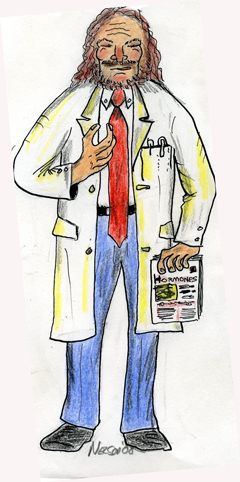
\includegraphics[height=60mm]{corps/chapitre17/img/personnage-bellavance.jpg}
\end{floatingfigure}

Alors lui, ce dépositaire d’une vie unique, potentiellement riche, ouverte à tout, une vie non renouvelable, non rebobinable, une vie de plus en plus monotone de médecin désabusé qu’il était en train de gaspiller au jour le jour dans une petite ville terne à côté d’une femme qui ne se promènerait jamais en string sur une plage brésilienne, lui qui n’avait jamais vu New York, Rio et Bangkok glissa tout doucement dans l’onirisme; il se mit à rêver de Delhi, Bali et Djara, à vouloir sentir, lui aussi, «les parfums de Chine» et le Sahara dans le souffle d’une belle. Il abandonna son quai et entra s’asseoir dans la taverne de l’imaginaire et de la fiction. Par personnages interposés, ceux de Jean-Marie Le Clézio, de Paul Auster, de Gabriel Garcia Marquez et de tant d’autres, il se créa des Saskatchewan qu’il quittait en train pour venir découvrir Montréal, des expéditions militaires en Égypte où il attrapait la vérole, une famille très étrange de Belleville dont il était l’aîné, une colonie de rats qu’il utilisait pour s’évader de la Bastille.

Mais il paraît que ceux qui aiment rêver passent leur vie à dormir. Voilà pourquoi, à 40 ans, il était devenu d’un ennui mortifère pour son entourage et qu’à 45, il s’était réfugié dans l’univers holographique quantique se modélisant des avatars en fonction des idéaux qu’il aurait tant souhaité vivre. Pourtant, le matin, quand il se regardait dans le miroir, il éprouvait la certitude, le temps d’une nanoseconde, «Time’s a loaded gun», qu’un jour, quelque chose se produirait, que sa vie si assommante, si mortelle, changerait. Qu’il vivrait vraiment. Envers et contre tous, il y croyait. Sinon, il se serait sûrement suicidé. Dieu sait qu’il en avait les moyens. N’était-il pas brillant et plein de ressources ?

Dans sa tête, il y avait constamment cette chanson essentielle de Brel qui trottait :

    Rêver un impossible rêve
    Porter le chagrin des départs
    Brûler d’une possible fièvre
    Partir où personne ne part

    Aimer jusqu’à la déchirure
    Aimer, même trop, même mal,
    Tenter, sans force et sans armure,
    D’atteindre l’inaccessible étoile

Alors quand à 51 ans, on lui avait parlé de ce projet de culture hormonale sur des corps cliniquement morts, il avait très rapidement fait taire sa conscience. Ces gens du ministère des Affaires gérontologiques avaient beau lui sembler de bien vils personnages, ils étaient LE pouvoir, ils avaient LES crédits et ils représentaient LA fin de sa triste vie inutile dans une petite ville ennuyeuse. En signant sur les pointillés, il faisait en sorte que désormais, il se passerait quelque chose, qu’il ferait les annales, que son nom serait associé, pour toujours, à un mini bond scientifique. Bref, Christian Bellavance s’était levé et avait quitté sa taverne.

Quant à sa «petite clause un peu particulière», il s’agissait simplement d’accepter de ne pas intervenir dans la mise en marché, la vente et la gestion financière du projet. Lui, il produirait les hormones, il trouverait des façons inédites pour en optimiser la fabrication et il gérerait l’aspect médical de l’aventure. On lui garantissait que tout excédent des revenus sur les dépenses serait versé au Centre afin d’améliorer le quotidien des bénéficiaires. À son âge et connaissant les humains, il n’y avait pas cru un instant. Mais, il avait enrobé ce doute certain de sept épaisseurs d’hypocrisie professionnelle, la spéciale résistante, celle qui se vend en contenants de deux litres dans toutes les forêts de gratte-ciel de la planète, et il était déménagé à Rimouski, laissant à Trois-Rivières épouse, ado, patients et voisins.

Dans des locaux du sous-sol initialement prévus pour les pensionnaires voulant se divertir en s’adonnant aux joies de la menuiserie légère, de l’électronique inoffensive, du tissage de catalognes, de la confection de lampes en papier de riz et de tous ces autres gossages de statuettes, le chercheur sur le retour d’âge s’était aménagé un centre de prélèvement, ainsi qu’un laboratoire, et on lui avait fourni le personnel nécessaire. Au bout de deux ans d’efforts, il avait récolté des résultats pour le moins spectaculaires. Il arrivait non seulement à obtenir le double de rendement par «corps souche» comme il appelait les semi-cadavres qu’on lui amenait, mais il réussissait à les maintenir en vie - un bien grand mot - trois fois plus longtemps qu’au départ de ses expériences. Il avait même un corps de vieille qui en était à son quatorzième mois de production.

Ce qu’on lui demandait surtout tournait autour de l’hormone humaine de croissance, la fameuse GH produite par la glande antéhypophyse, dite glande pituitaire antérieure. Le docteur Bellavance savait qu’on avait besoin de GH dans certains projets occultes de régénération ectopique d’organes vitaux, des projets dont dépendait le sort de certains patients très riches. Mais il savait surtout que certains laboratoires illégaux en achetaient de très grandes quantités pour en tirer des capsules de jouvence, des jujubes au goût de miel sensément capables d’agir comme agent anti-âge et antigras au risque des pires effets secondaires. Bien sûr, il y avait les hormones de synthèse, comme ces somatotrophines, lucratif fleuron du génie génétique de Monsanto. Mais on était loin de la qualité des vrais GH, même celles prélevées sur ces morts-vivants que le Centre lui livrait sur une base régulière.

Comme il n’était pas bête, il voyait bien l’écart entre les objectifs de production qu’il dépassait, mois après mois, et les résultats que Carl Michaud lui faisait remettre par Philippe Dauphin, sans jamais prendre le temps de lui expliquer quoi que ce soit. Il voyait bien qu’on l’assimilait à un exécutant sans grade et que les dividendes que son projet générait vraiment, on les lui cachait à coup sûr. En même temps, il constatait que l’ordinaire du CRG-BSL se détériorait sans cesse, ce qui signifiait, possiblement, que l’argent allait ailleurs.

Lorsque le sentiment d’être un rouage imbécile dans une magouille qu’il ne comprenait pas occupait toute sa tête, il se changeait les idées, cette fois non pas en se retirant dans son univers de fiction, mais en documentant, de façon maniaque, le déroulement de son entreprise. Ainsi, quand on lui donnerait le feu vert pour publier les résultats de sa recherche, il aurait tout en main. Il voyait déjà le titre : «Factor B : An Affordable Method to Optimize the Production of Human Hormones under Constant Clinical Supervision, by Professor Christian Bellavance, MD, FRCPC, FACP, Head of Research, CRG-BSL, Rimouski, Québec, Canada». Quel libellé ! «Factor B» ? Ne fallait-il pas brandir un magnifique «buzzword» à l’américaine pour référer à sa méthode ? «Factor B» sonnait bien, faisait professionnel et reprenait le «B» de Bellavance. Quant à «Professor», le titre se justifiait par le fait que le porteur avait été chargé de cours en techniques infirmières au Cégep de Trois-Rivières, durant … un semestre.

Tout cela pour dire qu’il fut à demi surpris quand il observa, sur une période de quinze jours, un employé de la direction des communications, Claude Sey, s’approcher de lui à la manière d’un requin faisant des cercles subtils. Il se doutait bien du sujet sur lequel le jeune homme finirait par l’entretenir, même si le prétexte était la préparation d’un document multimédia destiné à vanter les mérites du centre hormonal. Chattemite, le docteur se laissa manœuvrer, juste pour voir !

«Enfin, nous y voilà !» fut sa réponse lorsque Sey toucha au but pour la première fois.

- Quel est votre intérêt dans cette affaire ? Vous pouvez parler sans crainte, ici il n’y a ni caméra, ni micro, ni cafard, rien. Ça a fait partie de mes conditions quand on a construit.

Claude Sey plongea sans ambages.

- Je viens mettre mon nez dans vos tiroirs, docteur, parce que je ne sais pas trop quoi faire avec certaines informations.

- Quelles informations ?

- Les employés qui ont un bureau proche de celui de Philippe Dauphin – le mien est attenant - entendent parfois des bribes de conversation qu’il a avec Carl Michaud. D’une fois à l’autre, on finit par comprendre que votre projet serait une «machine à fric», une «mine d’or», la «passe du siècle». Mais en même temps, je m’excuse de devoir vous le répéter, vous seriez un «chercheur décollé de la réalité», un «naïf», un «lunatique» qui n’aurait aucune idée de ce qui se passe à deux pouces de son nez». Ça, c’est quand ils sont polis.

Bellavance ne sursauta pas.

- Vous n’avez pas répondu à ma question : quel est votre intérêt ?

- Si je lis attentivement les rapports que Michaud dépose au CA relativement à votre bébé, je vois qu’on y parle de «légers profits» ou de «profits prometteurs ». Guère plus ! Les entrées de fonds que vous générez, docteur, seraient à peine suffisantes pour couvrir vos coûts et pour justifier la continuation du projet. On est loin de la «machine à fric», de la « mine d’or» ou de la «passe du siècle» dont ils discutent entre eux. J’ai un gros doute à leur sujet; ça me ronge. Mon intérêt dans cette histoire ? Simplement de comprendre dans quelle galère je me suis embarqué en venant travailler ici. J’ai choisi le milieu gérontologique pour pouvoir contribuer, à ma façon, à améliorer leur sort misérable, pas pour cautionner une gamique.

- Et vous pensez, mon jeune ami, que je vais vous aider à vous faire une idée ? À apaiser votre conscience ?

- En vous parlant, j’ai couru le risque que vous soyez honnête. J’ai imaginé que vous saviez ce qui peut arriver, légalement, à des cadres qui boulechitent leur conseil d’administration, qui lui produisent des documents mensongers et qui brassent des affaires personnelles avec l’argent des contribuables.

Le médecin hésita, le temps de se fignoler une réponse à son goût.

- Nous allons arrêter cette conversation surréaliste, ici maintenant, monsieur Sey. Je pense vraiment que vous êtes mal servi par une imagination divagante à conséquences pathologiques. Prenez des vacances. Ça presse ! Au revoir monsieur.

Mais deux heures plus tard, il l’appelait en exigeant le mode confidentiel et lui donnait rendez-vous chez lui, le soir même.

Ce fut le début de plusieurs rencontres pendant lesquelles il fut possible de recouper l’information et d’obtenir des certitudes. Si, au terme, il manquait le montant réel des sommes détournées, on savait sans l’ombre d’un doute qu’une fraude était en cours. On savait notamment que le tandem Michaud-Dauphin avait confié la distribution des hormones à un ex-employé de Pete Barrett, un certain Julien «Djou» Dassilva. De plus, en passant des heures sur son terminal, Claude Sey avait trouvé des chiffres éloquents sur le marché des hormones naturelles. On savait maintenant qui les produisait, comment elles étaient expédiées, à qui elles se vendaient, en quelle quantité, à quelle fréquence et à quel prix. Même en coupant par dix la valeur marchande officielle, les rapports au CA auraient dû faire état de revenus de loin plus importants, compte tenu des quantités produites au sous-sol du CRG-BSL.

Ne restait plus qu’à déterminer la marche à suivre. Dans un premier temps, on rejeta l’affrontement direct avec la direction générale. On craignait de devoir se battre contre une organisation dont les ramifications s’étendaient en dehors du Centre. Le seul nom de Barrett avait de quoi faire frémir les moins timorés. On rejeta également l’idée de recourir à un membre du CA, un administrateur que l’on documenterait pour qu’il puisse poser des questions embarrassantes. Le seul qui semblait parfois faire preuve de résistance face à Michaud était Jean-Michel Desrosiers, un comptable de Rimouski qui, par ailleurs, était trésorier de comté pour le Parti libéral du Québec dont le patron était l’affreux Barrett. La police ? C’était courir au suicide professionnel. Encore ici, le dossier se serait retrouvé à plus ou moins brève échéance sur le bureau de Barrett. On décida plutôt d’étendre la base, de se mettre en situation de ne pouvoir compter que sur deux têtes, de former un groupe d’employés honnêtes et capables de se tenir debout, une sorte de «Comité du salut public» dont les membres auraient dépassé leur seuil de tolérance quant aux exactions et autres magouilles qui sévissaient dans l’établissement. Peut-être que là, en élargissant les ressources, les jeux de contacts, les possibilités d’entraide, on arriverait à quelque chose. Encore fallait-il être extrêmement prudent.

Mais qui dans une boîte aussi corrompue que le CRG-BSL pourrait correspondre au profil recherché ? Qui sinon certains marginaux comme Sébastien Larose, le dernier syndiqué de la fonction publique du Québec, Jipé Gendron, alias Tit-mononk, un résident en 2P qui représentait les bénéficiaires au Comité de déontologie, Robespierre Alcide, un tabletté statutaire qui passait ses journées à s’occuper d’on ne sait trop quoi, Vlado Markovsky, le directeur de l’informatique qui semblait en avoir plus qu’assez de la situation cybernétique, Shimoune Saint-Pierre, un homosexuel qui prenait plaisir à enquiquiner les pires éléments du Centre, Ophélie Marcotte, la jeune collègue de Saint-Pierre ou encore, Timothée Tardif, un CS-1 plein de compassion pour ses pensionnaires, mais dont tout le monde se moquait ?

- La clé à tout ce beau monde pourrait être Tardif, fit Claude Sey qui, avec l’aval du docteur, s’engagea à amorcer une manœuvre d’amorce circulaire auprès de lui, comme il savait si bien le faire.

Ce qui avait été fait, la semaine dernière, au sortir de la réunion mensuelle du Comité de déontologie.

Mais aujourd’hui, Christian Bellavance rumine dans son bureau avec. Comme à son ordinaire, du Brel comme trame sonore.

    Les vieux ne meurent pas, ils s’endorment un jour et dorment trop longtemps
    Ils se tiennent par la main, ils ont peur de se perdre et se perdent pourtant
    Et l’autre reste là, le meilleur ou le pire, le doux ou le sévère
    Cela n’importe pas, celui des deux qui reste se retrouve en enfer
    Vous le verrez peut-être, vous la verrez parfois en pluie et en chagrin
    Traverser le présent en s’excusant déjà de n’être pas plus loin
    Et fuir devant vous une dernière fois la pendule d’argent
    Qui ronronne au salon, qui dit oui qui dit non, qui leur dit : je t’attends
    Qui ronronne au salon, qui dit oui qui dit non et puis qui nous attend.

- Quand même !

Il regarde son terminal.

- Arrêt ! Autre arrangement ! Jazz ! Oui !

Chick Corea vient instantanément prendre la relève de l’immortel Wallon.

Débarrassé de sa distraction, le docteur comprend que la conjoncture s’est un peu complexifiée. Sey a été congédié; il n’a plus accès au Centre. Quant à Tardif, il n’a voulu rien entendre la veille. Mais il y a ce grand noir, cet Alcide, et cette pédale, ce Saint-Pierre, qui, à en croire Sey, auraient la confiance du chef de section. Et il y a les flics dans la boîte depuis hier ! Il y aura sûrement enquête. Michaud et Dauphin doivent être sur les dents. Le moment d’agir, du moins d’élargir le cercle pourrait être bon.

Puisqu’il faut battre le fer quand il est chaud, le chercheur quitte l’air glauque de son antre et monte vers la cafétéria. L’heure du petit déjeuner est presque finie et Saint-Pierre ne semble plus servir sa saloperie de manger mou. Il est même en train de discuter le bout du gras avec Alcide. Dans le vaste réfectoire, quelques vieillards flânent, des bénévoles ramassent les traîneries, d’autres nettoient la fontaine, essuient les dessus de table et replacent les chaises. À cette heure, se dit Bellavance, le conciliabule devrait bientôt se terminer. Le mieux est d’attendre dans le couloir, mine de rien, espérant voir apparaître l’un ou l’autre, ou les deux.

Bingo ! Voilà le colosse à la profession inconnue qui se pointe.

- Monsieur Alcide, le hèle-t-il.

Robespierre se retourne.

- J’ai bien l’honneur de porter ce nom. Et vous, monsieur, vous êtes ce docteur Bellavance qui travaillez au sous-sol pas trop loin des Tontons Macoutes, ces gens inquiétants qu’on surnomme ici Papyblues, mais que moi j’appelle Tontons Michauds.

- Je vois que vous faites dans l’humour noir, monsieur Alcide …

- Ouh ! qu’elle est cherchée celle-là !

La partie ne sera pas facile, oh que non !

- Bon, trêve de mondanités, je n’irai pas par quatre chemins. Hier j’ai essayé de dire certaines choses importantes à votre ami, monsieur Tardif, mais il n’a pas voulu les entendre. C’est dommage !

- Par les temps qui courent, Timothée en a plein les bras, le pauvre. Il ne sait plus trop où donner de la tête.

- Remarquez, ces choses, je pourrais vous les révéler à vous, vous en feriez ce que bon vous semble. Et, croyez-moi, vous serez en mesure de convenir que je ne vous aurai pas fait perdre votre temps.

- Quelles choses ?

- Mon bureau est un des rares endroits de ce centre, monsieur Alcide, où on peut parler sans danger. Passez me voir quand vous le voudrez.

- J’ai des disponibilités, maintenant.

- Dans ce cas, si vous voulez me suivre.

Quand, une demi-heure plus tard, Robespierre remonte aux étages, il a un topo complet en tête, celui d’une machination bien installée à la direction générale, où le docteur Bellavance fait figure de dindon de la farce. Quelques mots lui viennent à l’esprit dont exaction, gamique, concussion, tripotage, combine et, son préféré, prévarication.

- Madame Bellow, vous semblez en grande forme ce matin, fait-il en direction de l’ex-bibliothécaire occupée à fournir en livres, une quinquagénaire d’assez fraîche date qui, juchée sur une chaise, emplit la tablette du haut.

Dès le lendemain de l’affectation de Bea Bellow chez l’administrativement inutile Robespierre Alcide, des étagères en métal bêtement entreposées au sous-sol lui avaient été livrées, une gracieuseté du tout aussi inutile Sébastien Larose qui était copain-copine avec la responsable du mobilier, l’immémoriale Louise Lavoie. Rien n’échappait au contrôle de cette ancienne noceuse recyclée, avec responsabilités gestionnaires, dans le bric-à-brac institutionnel; ni les chaises bancales, ni les bouts de planche non utilisés, ni les tables de travail désaffectées, rien ! Aucun cadre décoratif, restant de peinture, chariot et téléviseur, aucune patère, tablette, retaille de tapis, poignée, serrure électronique et autre crédence, ne lui étaient étrangers. Quand elle entrait dans une officine, l’occupant avait l’impression qu’elle en connaissait intimement chaque objet et qu’il pouvait s’en faire déposséder en un clin d’œil.

- Le vrai pouvoir, aimait-elle répéter, ce n’est pas d’occuper le bureau du directeur général, mais d’en contrôler le mobilier ! Car privés de chaise, les trous de culs deviennent vulnérables !

Les mains sur les hanches, le sportif poursuit ses politesses.

- Et vous, madame Lavoie, vous êtes venue aider madame Bellow ? Quelle gentillesse ! En plus, vous me semblez toute primesautière.

- Primesautière, de quossé ?

- Frétillante, pimpante, fringante ?

- Faut ben. Dites donc vous, vous en avez donc b’en des livres ? Les avez-vous tout’ lus ?

- Oui ! Mais là, maintenant, j’en cherche un d’Henri Amouroux.

Bea Bellow, cesse un instant son petit manège et tape des mains.

- Là-bas, deuxième tablette, vers la gauche, reliure jaune.

Robespierre a tôt fait de repérer le bouquin, de le feuilleter fébrilement, d’émettre un grand ahhh! et de scribouiller sur une feuille qu’il se dépêche d’aller coller à sa porte. On peut y lire :

    Le drame des dictatures, c’est qu’elles donnent toute licence aux malades mentaux, aux mégalomanes, aux méchants, aux malhonnêtes gens d’aller jusqu’au bout de leur folie, de leur mégalomanie, de leur méchanceté, de leur malhonnêteté.

- Aussi bien afficher ses couleurs ! sourit le gaillard en se tapotant la boucle d’oreille.

Sans délai, il entre en communication avec Marie-Odile Tremblay.

- Écoute, je me demandais, comme ça, si c’était possible de te parler sans gadget, ni cafard, ni témoin, genre maintenant, tout de suite ? J’ai un truc qui va sûrement t’intéresser.

- C’est possible, t’as juste à passer à mon bureau.

Le ton est maussade. Il tente d’égayer.

- J’ai suffisamment de gènes afro-américains dans le corps pour savoi’ que les pauv’es noi’s ont inté’êt à ne pas fwéquenter les commissa’iats de flics !

- C’est ça, fais le cave !

Pas en forme, la matrone !

- J’ne rigole pas. Dis, pourquoi on n’irait pas prendre l’air, en haut, sur le toit ? C’est agréable, il fait beau, y a des chaises, des balançoires, de belles fleurs, le décor parfait pour jaser de mes affaires ?

- Coudon, t’es-tu parano, toi ?

- Je te prends peut-être dans un mauvais moment ? Je peux te rappeler plus tard ?

Marie-Odile se revoit, hier soir, retourner chez elle, seule, défaite, frustrée, en colère, jalouse à en avoir mal au ventre, une douleur moins supportable encore que celle de ses menstruations difficiles. Elle se revoit vouloir ouvrir sa porte d’appartement à grands coups de pieds et se retenir in extremis. Elle se revoit en train de maudire ce Timothée, l’idiot du village sur qui elle est tombée, et qui, malgré sa dégaine, la rend déjà malheureuse. Évidemment, si elle était moins possessive, défaut épouvantable, elle le sait, qui, à ce jour, a ruiné le peu de relations amoureuses qu’elle a connues, elle n’en aurait possiblement rien à glander. Effectivement, pourquoi cet homme ? Il y en a pourtant bien d’autres. Parce qu’il est un homme avec tout l’attirail nécessaire ou parce qu’il est Timothée, avec toute sa gentillesse de perdant ?

- Bof !

- Tu ne perdras pas ton temps.

Pourquoi pas !

- Bon ! C’est comme tu veux. Je monte.

- Pas de gadgets électrochoses ?

- Pas de gadgets.

- Promis ?

- Promis, bougonne celle que les employés surnomment la Bitch.

Il faut à Robespierre, écrasé dans une chaise de parterre, ses longues jambes sur une autre, un bon cinq minutes pour bien raconter la fraude dont se dit exécutant involontaire le docteur Bellavance. Marie-Odile, assise les fesses serrées sur le rebord d’une table, semble réfléchir.

- Il t’a fourni des preuves ?

- Des rapports au CA qui n’ont rien à voir avec sa vraie production. Des déductions. De quoi intéresser les enquêteurs. Ça sent la chiotte en train d’se boucher.

- Pourquoi tu me contes ça ?

Si l’âme du sieur Alcide était aussi limpide que celle d’un nouveau-né, il répondrait «pour mieux de sauter, mon enfant !» Mais voilà, Robespierre est un adulte de 2033 qui accomplit son sacerdoce quotidien dans le remugle du CRG-BSL. Il parle donc d’une mainmise sur l’établissement par une clique de malfaiteurs, dont les éléments les plus visibles sont Carl Michaud et Philippe Dauphin. Ce sont des gens qui grattent partout pour économiser, ce qui leur permet de mieux empocher. Tout cela, bien entendu, se fait au détriment des bénéficiaires à qui on a presque tout coupé. Le gymnase a été trafiqué en salon des employés, le centre de bricolage en atelier pour le docteur Bellavance, la piscine condamnée, la très belle terrasse sur le toit, interdite, la climatisation réservée aux deux étages administratifs, le personnel de nuit charcuté à sa plus simple expression, les vieux logés en dortoirs 2P souvent obligés d’aller changer les couches dans les salles palliatives, sans parler de cette saloperie de Nutrisuz, le foutu manger mou que fait préparer l’ignoble Amédée Chicot, un autre parasite associé à la magouille. Or, avec le trafic présumé des hormones de culture, c’est à la veille de sauter; quelqu’un quelque part va finir par tout comprendre. Et le jour où cette révélation frappera, dans une semaine, dans un mois, dans un trimestre, beaucoup de hauts gradés auront à choisir leur camp et à montrer patte blanche.

Le problème est simple :

- Si on attend que ça pète, parce que ça va arriver, on ne pourra rien pour aider Timothée qui est aux prises avec une histoire kafkaïenne.

- Je te suis pas.

- Je dis que si on se met en mode proactif, qu’on fasse crever l’abcès, on n’sera pas trop loin des commandes quand viendra le temps de sauver Marie Rioux et Romain Tardif.

La fille Tremblay voit passer devant elle l’image de ses propres parents, celle de son père usé, mal en point, celle de sa mère, angoissée, craintive.

- Qu’est-ce que t’entends par «faire crever l’abcès» ?

\begin{floatingfigure}[l]{30mm}
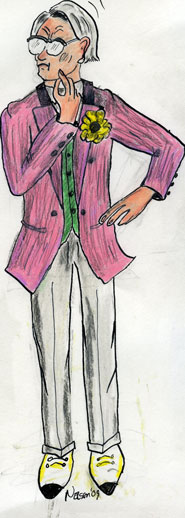
\includegraphics[height=60mm]{corps/chapitre17/img/personnage-carl.jpg}
\end{floatingfigure}

- B’en, on commence à avoir en main une couple de dossiers faciles à documenter et pouvant mener ces salauds au gibet. Il suffit de bien s’en servir ! J’imagine Carl Michaud, la corde au cou, avec son veston vieux rose, ses lunettes d’intello, sa ‘tite coupe de cheveux kioute et ses godasses de banquier 1900. Bordel !

Elle le regarde, les yeux plus plissés que la normale, ce qui est assez près de la grimace.

- Une «couple de dossiers» ?

Robespierre avait prévu le coup.

- OK, je vais t’asséner l’essentiel d’une deuxième histoire à relents de fosse septique.

Y prenant autant de plaisir que s’il avait été en train d’amuser des enfants à l’Heure du conte, l’arrière-petit-fils de l’inventeur du Petepano narre à l’Ilsa-de-Timothée l’invraisemblable découverte de Shimoune Saint-Pierre, ajoutant, hypocrite, force détails scabreux, incluant la dysfonction érectile de Pete Barrett.

- On a plein de clips qui nous présentent, bien en santé, les parents pourtant décédés du Gros Turcotte. On sait que ce pavillon est financé par l’État et qu’il abrite des illégaux intimement «plogués» sur cet immonde goret.

Robespierre s’est emporté et Marie-Odile est sidérée.

- Astie !

- Je t’le fais pas dire, ma belle !

Si l’expression «roucouler des yeux» était consacrée, quelqu’un en autorité l’aurait consignée dans un ouvrage officiel comme signifiant «Mouvement soutenu d’une paire de grands yeux noirs destinés à renforcer d’une façon frôlant l’indécence, le non-dit sexuel de propos relatifs à autre chose.» Bref, malgré l’orientation de la conversation à donner la chair de poule, Robespierre devise la bite sous le bras. On ne se refait pas.

Au même moment, Timothée est assis à l’arrière d’un taxi en train d’expliquer au chauffeur que pour la première fois de sa vie, il est en retard au boulot.

- Grosse soirée, mon jeune homme, ausculte Jawad Kebbaj.

- Je viens de me réveiller; j’ai même pas pris l’temps de manger.

Le bonhomme fouille dans un sac, sur le siège à sa droite, et en ressort une clémentine.

- Tiens, mange au moins ça.

- Euh, je sais pas si je dois …

- Écoute mon jeune homme, la clémentine est le cadeau du Maroc à l’humanité entière. Si tu veux insulter un Marocain, refuse la clémentine qu’il t’offre. P’is un Marocain insulté, c’est très très dangereux. Ouh la-la !

- En ce cas, je vais m’incliner. Merci monsieur Kebbaj.

L’agrume en main, Timothée entre au Centre et s’enligne vers les ascenseurs. Ce faisant, il croise le gros Lavoie, canaille sévissant comme préposée au 6e Nord. Le taupin le regarde, l’air narquois.

- Bonne nouvelle pour toi, le Motté, t’auras p’us à nous ramener la mére Morency.

Comme le CS-1 ne réagit pas, l’obèse enchaîne.

- On s’est écœuré et on l’a crissé en SP. A va décoller dans un sac zippé à la prochaine cérémonie. L’incinérateur, bye-bye ‘stie !

Instantanément, Timothée se rue sur Lavoie. Vociférant tel un schizophrène en crise, il le pousse sur le mur et le repousse à chaque fois que le misérable tente de rétablir sa dignité. De toute évidence, il a perdu le contrôle de ses émotions et, dans ses hurlements, on peut sentir l’expression de son impuissance face à une décision définitive prise un étage en haut du sien, une décision sur laquelle il n’a aucun droit de regard. C’est Shimoune Saint-Pierre qui, arrivé à la course, se saisit du forcené, un forcené dont la colère est telle qu’il doit fermement l’emprisonner par-derrière, dans ses bras puissants, et l’entraîner à grand fracas vers la cafétéria. Inutile de dire que dans le couloir, plus personne ne bouge ni ne parle et que tous vont se souvenir longtemps de cette violente éruption de rage sourde.

- Câlisse, Shimoune , ils vont tuer madame Morency, crie-t-il en déplaçant une table d’un coup de pied, ce qui, dans un vacarme amplifié par la vastitude du local, fait tomber deux chaises.

Quelques vieillards désœuvrés se dépêchent de filer.

Comme il se doit, la patience à toute épreuve de la «Grande folle du manger mou» arrive à calmer le malheureux chef de section, à le faire se ressaisir et, surtout, à le faire asseoir.

- Veux-tu une limonade ? Un thé ?

- Ça n’a plus de maudit bon sens, Shimoune, chigne son ami. Faut absolument faire quelque chose. Crois-moi, j’vas tout casser, j’vas tout arracher. C’est pas vrai que j’vas les laisser faire ça.

Le préposé au Nutrisuz tapote son dispositif personnel polyvalent.

- Allô dieu d’ébène ? As-tu une minute ? Oui ? Peux-tu descendre ici à la cafétéria ? Timothée a besoin d’aide; c’est sérieux. Il est arrivé un bordel. Oui mon chou, une bagarre. Ne-non ! Moi ? J’ai encore une demi-heure à tirer, y a du bon manger mou à servir, miam-miam ! Merci. Je t’attends, chou.

Sur le toit du Centre, Robespierre s’excuse auprès de Marie-Odile.

- Il est arrivé quelque chose à Timothée, faut que j’aille le chercher à la cafétéria.

- Quoi ?

- Une bagarre. Il est un peu, euh, désorganisé.

Si la femme flic est immédiatement allumée par le mot «bagarre», phénomène excessivement rare dans un établissement gériatrique, la femme tout court l’est encore plus par le fait qu’il s’agisse de Timothée, cet éternel perdant qui l’a fait rager hier soir.

- Je te suis.

Quand il les voit arriver, Timothée regarde Shimoune, secoue la tête et se lève. Il a compris. En silence, sans un regard pour Marie-Odile, épreuve qui lui semble infranchissable, il serre de près ses amis vers l’ascenseur. Au 5e, ils foncent tous trois vers le bureau de Robespierre, sans s’occuper de Ronnie Ross qui veut parler de l’Illuminé – «il a fait un ACV» - ni du vieux Jean Saint-Gelais qui, à l’instar de ceux qui savent des choses sans les dire, arbore un rictus entendu, même s’il n’a jamais vraiment su grand-chose.

D’un commun accord, Béa Bellow et Louise Lavoie laissent entrer les trois envahisseurs et se glissent silencieusement vers le couloir.

L’agente de sécurité fouille dans son bermuda et finit par retrouver son petit zinzin noir sur lequel, du pouce, elle exerce une pression.

- Tout est maintenant brouillé. À c’t heure, raconte ce qui s’est passé.

- J’ai pété ma coche, lui répond Timothée. Le gros Lavoie m’a annoncé avec le sourire, qu’ils avaient placé madame Morency en SP et qu’elle serait gazée et incinérée à la prochaine cérémonie de groupe. Ça se peut pas ! Faut que j’arrive à empêcher ça.

Robespierre s’écrase dans son fauteuil et, les yeux fixés au plafond, émet un puissant bâillement.

- OK, trop c’est trop ! On clenche !

Il baisse les yeux vers Marie-Odile.

- T’es avec nous ?

- C’est qui, ça nous ?

- Pour l’instant, Timothée, Shimoune, moi. Tantôt, on va rajouter le docteur Bellavance et Claude Sey.

- On clenche comment ?

- C’est à voir, faut en jaser. T’es une experte en sécurité, tu peux sûrement nous aider.

- Moi ?

- B’en oui !

L’air renfrogné que la femme flic arborait jusque-là semble s’estomper.

- Faut que je voie vraiment le dossier qu’a le docteur Bellavance. Si c’est ce que tu dis, s’il y a matière à porter des accusations au criminel, c’est certain que j’embarque.

Robespierre brandit ses deux pouces en avant de lui.

- Yes !

Tous trois conviennent alors de rencontrer le médecin, idéalement chez lui, question de se faire une idée finale et, de là, se définir une stratégie d’attaque. Les humains étant ainsi faits, les gestes décisifs sont toujours posés par une infime minorité, des gens qu’on appelle leader, fonceur, bélier, chef, boss, capo, édile, adjudant-chef, maître, producteur, propriétaire, tennô, padrino, président, pape, directeur, foreman, caudillo, ministre, prédicateur, meneur, auteur. Mais ici, ils ont pour nom Robespierre Alcide, monument de force et de sagesse sur qui deux paires d’yeux sont fixées. Ce que voyant, l’armoire à glace pitonne sa boucle d’oreille.

- Docteur Bellavance, ici Robespierre Alcide. Peut-on parler de façon confidentielle ? Merci. Dites, je suis avec des amis et nous souhaiterions nous entretenir avec vous. Auriez-vous du temps, ce soir ? Oui ? Parfait. D’accord. Ça marche, 19h30 chez vous. Oui. Nous serons quatre. Ah ! Timothée Tardif, Shimoune Saint-Pierre et Marie-Odile Tremblay. Oui, l’agente de sécurité. Non, pas de problème. Je vous le dis. Parfait. Au revoir, docteur.

Il se recule dans sa chaise et étire ses longs tentacules.

- C’est parti !

S’il le pouvait, il prendrait Timothée dans ses bras et lui jurerait que plus personne ne pourrait désormais faire brûler de petits vieux, les nourrir à la soupane chimique, les vêtir comme des cloches, les traiter comme des demeurés. Il lui promettrait que ses parents, Marie et Romain, seraient délivrés de leur sous-sol poussiéreux, qu’ils pourraient vivre au grand jour sans devoir aller se cacher avec les autres sur l’île d’Anticosti. Il l’assurerait que les méchants qui commandent l’établissement seraient traqués, arrêtés, condamnés et écroués dans la plus humide des geôles en compagnie des Papyblues et autres Tontons Michauds, que le gros Turcotte serait traîné sur le banc d’infamie, puis accroché par le cou aux fourches patibulaires avec les boyaux du fraîchement éviscéré Pete Barrett. Mais on est en public, un public aux yeux inquisiteurs, plissés et, quelque part, bleus, dont la porteuse en uniforme de la Sécu semble en réflexion carabinée.

- J’m’en vais me coucher à la maison, soupire Timothée. Y a rien à faire avec moi, aujourd’hui.

- C’est correct, mon ami, repose-toi bien. J’vais passer te prendre à 19 h.

Dans le couloir, Ronnie Ross finit par le rattraper.

- Motté ? Je fais quoi avec l’Illuminé ? J’l’envoie en SP ?

- Non câlisse ! On n’enverra plus jamais personne se faire incinérer ! Fie-toi sur moi, Ronnie !

Ce dernier réalise que son chef, parvenu aux ascenseurs, n’est plus ce bon vieux Motté auquel il a été habitué. Il lui crie :

- Oui, mais je fais quoi avec ?

- T’appelles les secours, tu le fais soigner, comme un être humain !

Le préposé n’en croit pas ses oreilles. Mais il est trop tard, Timothée est déjà disparu.

Quand Robespierre passe le prendre à 19 h, le fils Tardif a l’impression que cinquante millions de caisses de clémentines marocaines lui sont passées sur le corps, même s’il a dormi un bon cinq heures. Mais il est serein, presque heureux. C’est qu’en se réveillant, il s’était fait un café et était descendu juger de l’état des choses chez ses parents. Stupéfait de ne pas entendre Gazou gronder comme un enragé, il en avait vite compris la raison en apercevant Béatrice en train de parler avec sa mère. Depuis quand y était-elle ? Il n’avait pas osé s’informer, se contentant d’en éprouver un grand bonheur. Il avait salué, puis retourné son sourire à la belle infirmière et, affreusement gêné, était reparti chez lui.

En arrivant devant la résidence du médecin, ils remarquent Marie-Odile dans sa voiture électrique qui les attend, avec Shimoune appuyé nonchalamment, les coudes sur le toit.

- Dieu du ciel, madame, comme ce soleil de fin de journée convient à votre carnation et à la dorure de vos cheveux. Jusqu’à la fin de mes jours, je serai redevable à l’astre de vie d’un tel spectacle.

La femme flic sourit presque au géant.

C’est Claude Sey, jeune idéaliste fraîchement congédié, qui, en se servant du quanticordi de la maison, se fait un devoir de présenter à Marie-Odile l’accablant dossier qu’il a accumulé. Puis, d’un commun accord, Shimoune relate sa ballade bicoise menant à la découverte d’un refuge pour illégaux hautement subventionné. Il a des clips et des photos. Autrement dit, résume Robespierre, on a en main de quoi faire «sauter la marmite». Encore faut-il savoir comment et quand.

- Ça va, marmonne Marie-Odile. Ça me suffit, j’vous suis !

Robespierre lève les bras vers le ciel face auquel il hoche la tête en signe de remerciement, imitant en cela bien des gens à qui son arrière-grand-père avait redonné du tonus.

- Il faut sauver Luce Morency, rappelle Timothée d’une voix presque inaudible.

- Oui, mais il faut surtout sauver les bénéficiaires du Centre, corrige Claude Sey.

- Il faut aussi sauver vos parents, monsieur Tardif, ajoute le docteur.

- B’en beau, mais il faut surtout clouer ces pourris sur une porte de grange, gronde Shimoune .

C’est alors que la petite société a droit à du grand Robespierre. Du Robespierre comme il ne s’en était pas vu depuis les premières années du Petepano. On le sait tous, la marque d’un chef s’imprime dans de tels moments. Laissant s’établir un silence d’alinéas, le tabletté le plus musclé de l’est du Québec prend la parole comme s’il se tenait dans la tourelle d’un véhicule d’assaut relié par communications holographiques à une brigade blindée.

- Madame, docteur, messieurs, j’aurais une démarche assez précise à vous proposer, pourvu que nous nous mettions d’abord en accord sur un aboutissement.

Le Québécois de lointaine souche antillaise fait alors valoir un point de vue selon lequel si on se contente de judiciariser les malfrats, ce qui pourrait ne pas être vraiment compliqué à réussir, «n’est-ce pas Marie-Odile», on ne serait guère plus avancé si de nouveaux escrocs venaient assumer la direction du Centre et que les personnes âgées continuaient de souffrir.

- Non, madame, docteur, messieurs, il faut plutôt s’assurer d’exercer soi-même le pouvoir. Et j’ai un plan.

- Un autre que moi, Monsieur Alcide, pourrait croire être en présence d’un militaire putschiste de l’Afrique.

- Docteur, vous êtes off. Mon idée est de laisser ces gens en place, mais de les contrôler avec la menace constante de les détruire. Ma proposition est de les forcer à tout réformer pour qu’ils deviennent des héros et qu’ils s’enferrent à tout jamais dans leur gloriole. Oui, docteur, je veux, avec vous, exercer le pouvoir, mais en tirant les ficelles dans l’ombre. Si mon plan fonctionne, il va me falloir, jusqu’à la fin de mes jours, tenir un colt 45 armé sur la tempe du gros Turcotte et un autre sur celle de Carl Michaud.

Marie-Odile est très impressionnée.

- On t’écoute Robespierre.

Elle a presque souri.

Le colosse regarde son assemblée et s’étire les muscles du cou.

- Avec votre indispensable collaboration, madame, docteur, messieurs, voici ce que nous pourrions faire, dès demain.

Dehors, sous le chaud reflet du soleil couchant, deux anonymes qu’on dirait endimanchés pour participer à des séances de torture filment les véhicules stationnés devant la résidence du docteur Bellavance. 
\chapitre{La fille sous la lanterne, le jeudi 28 juillet 2033 }{Toute la nuit,}{ Timothée rêve de manœuvres militaires. Ici une légère avancée avec attaque par le flanc droit, là un repli stratégique avec récupération de deux lance-flammes, encore ici une infiltration en pleine nuit de la ligne ennemie, le couteau entre les dents, et là, un enfouissement précipité dans le sol sablonneux. Le colonel Robespierre Alcide est partout en train de dicter des ordres dans son microphone de casque, de pousser sur des traînards aux yeux hagards, de chapitrer ses subalternes immédiats, de s’adonner au cliché cinématographique du genre «ils font quoi les connards de l’aviation ?» ou «pourquoi c’est toujours ma pomme qui hérite de la pire bleusaille ?» ou «il va falloir rapporter des dommages collatéraux !». Des tirs de mortiers ajoutent à l’ambiance sans faire de dégât, des fusées éclairantes couvrent de magenta orangé le terrain de manœuvre, des nuages de fumée à forte odeur pour abréger la souffrance de ses frères : morphine en injection, air comprimé et tout le cirque.  }

Sans se soucier du métal qui hurle à des vitesses folles au-dessus de lui, charriant parfois une tête, une jambe, une épaule, le brancardier Tardif saute de trou en trou. «Faut que tu bouffes», lui crie, confortablement assis dans le sien, Shimoune Saint-Pierre, caporal d’intendance, en lui lançant un carton non recyclable de Nutrisuz. Mais soudain, le sergent Tremblay, Marie-Odile de son prénom, saute dans leur planque. « Qu’est-ce que vous foutez ici en train de bouffer, mes salauds ? On s’entretue là-bas ! Votre compte est bon !». Mais au moment où elle bondit pour retourner au casse-pipe, un shrapnell lui arrache la moitié gauche du visage emportant avec lui la majeure partie du cerveau. «Elle pourra plus nous faire fusiller», fait remarquer Shimoune en mâchouillant, pour le principe, une bouchée de manger mou. «Le Motté, c’est à toi !», lui hurle Ronnie Ross troué de balles, mais encore accroché à sa sulfateuse .50. Timothée rampe jusqu’au moribond, le dégage de la lourde mitrailleuse et, les yeux sur l’inutile collimateur, commence à faire feu des deux poignées.

\begin{floatingfigure}[l]{50mm}
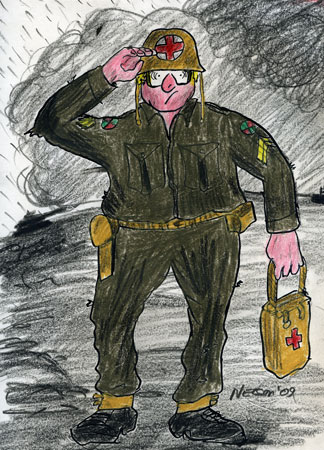
\includegraphics[height=60mm]{corps/chapitre18/img/personnage-timothee-guerre.jpg}
\end{floatingfigure}

Loin en avant, une silhouette se dessine dans la brume et avance dans la pestilence. «Arrête, Timothée-Milet ! Arrête ! On a gagné !», C’est sa mère, la Maririou, archet en main, mais sans son violoncelle. Pataugeant autour d’elle, Gazou a une main arrachée entre les crocs, la main d’un malheureux que les troupes du gros Turcotte ont déchiquetée. «Attention, maman, faut que je tire !». Mais elle continue d’avancer avec sa sale bête, les rafales de .50 lui sifflant à deux millimètres du casque. « Arrête Timothée, arrête, elle t’aime !». Le mitrailleur à la croix rouge s’étire le cou et aperçoit Béatrice en grand uniforme de major, les médailles faisant clinc-clinc. «Béatrice, je ne suis pas un fantassin, je suis un paramédic ! Sors-moi d’ici ! Si tu le fais pas, je vais mourir.» Et la belle l’aide à se lever et, comme si un écran antimétal avait cuirassé la lumière de son aura, l’entraîne sous sa protection vers l’arrière.

Puis il se réveille. En sueur ! Il est 4h45 et déjà certains oiseaux, possiblement les plus affamés ou les moins bien juchés, ont commencé à chicaner l’aurore qui tarde à lancer son travail de mise en lumière. Il ouvre silencieusement sa porte et constate que la rue Crouet sert de canal à une délicate brise bien tempérée par la chaleur des terres plus au sud. Décidément, les temps sont d’une clémence jamais vue. Rien à voir avec les étés précédents o`1 il a surtout éyé question de pluie, d’orages, d’averses et d’inondations. 4h45 ! Plus de sept heures à tirer avant qu’il ne se rapporte, ici même, au colonel Alcide pour les manœuvres devant débuter à midi. Il en sera ainsi pour Claude, Marie-Odile et Shimoune, lequel s’est fait remplacer par Ophélie Marcotte pour la journée. Trop tard pour reculer.

Un chanson lui revient à l’esprit quand il referme sa porte pour s’en aller à la douche.

    Vor der Kaserne
    Vor dem großen Tor
    Stand eine Laterne
    Und steht sie noch davor
    (Devant la caserne
    Quand le jour s’enfuit,
    La vieille lanterne
    Soudain s’allume et luit.)

Le pire, c’est qu’une heure plus tard, en franchissant à pied les quelque cinq kilomètres le séparant du Centre, «Wie einst Lili Marleen», celui de la voix chaude de Marlene Dietrich, lui restera collé dans le creux de l’oreille tout au long de sa balade et même plus. Il aura beau s’efforcer de ne penser qu’au plus horrible de ses cauchemars, il ne pourra s’en débarrasser. Même quand Jawad Kebbaj stoppera son taxi près de lui au début de la rue Sirois.

- Mais qu’est-ce qui se passe, mon jeune homme ? On affame le petit commerce, on n’utilise plus les services du vieux Jawad ?

- Bonjour monsieur Kebbaj. Je profite du beau temps pour marcher jusqu’au travail.

- Tu fais bien, c’est bon pour ta santé, tu fais bien. Tu vas vivre plus longtemps et rester mon client plus longtemps, Masha’Allah !

Quand à 6h15, il arrive «vor des Kaserne», c’est-à-dire devant le Centre, pas un chat ne bouge, personne ne se montre le bout du nez. Seuls des goélands en bande anarchique animent le décor. Mais à l’intérieur, la vie commence à donner des preuves qu’elle bat vraiment. Surtout quand il se pointe au 5e étage où Octavio Torres, un préposé de nuit, l’accueille avec la circonspection d’un douanier de Tijuana en présence d’un visiteur de San Diego.

- Hola Senor Jefe, una gran desgracia … votre bénéficiaire, Jean-Roch Savoie, le lit no 8 de votre SP, il a fait du bordel une partie de la nuit et il est mort tout à l’heure. Il a empêché tout le monde de dormir. Hijo de puta !
L’Illuminé a donc passé l’arme à gauche. Mort faute de traitements significatifs. Mort d’ennui, de déception, de frustration et de rage.

- Merci monsieur Torres, je vais m’en occuper.

Pour l’instant, il n’y a rien à faire, les préposés du grand frigo n’arrivant au boulot qu’à 8 h. Dans la salle palliative, la grogne de ceux qui en sont encore capables est à son comble. Timothée fait le tour de ses grabats pour essayer de calmer ce qu’il peut et s’arrête devant celui de Jean-Roch Savoie, l’homme qui connaissait sa Bible par cœur. Il s’approche du cadavre et, ramassant drap et couverture éparpillés comme à la suite d’une tornade, l’abrille respectueusement et lui joint les mains sur le livre saint qu’il a retrouvé sous le lit. J’ai d’l’argent pour toi, mon garçon.

La voix est celle d’un paquet d’os que plus personne ne lave et qui gît dans la couchette voisine.

- Dormez, monsieur Logan, il n’est pas encore 7 h.

- Je te vire 750 piastres, siffle le pitoyable vieillard, si tu me débarques de la prochaine cérémonie.

Timothée a soudainement envie de hurler, de donner de grands coups de pied dans la fourmilière.

- Écoutez-moi bien, monsieur Logan. Tant que je serai là, y a personne qui va vous amener à la cérémonie. Personne ici n’ira à la cérémonie. Il y en aura p’us de câlisse de cérémonie, c’est-y clair, ça ?

- J’te dis que j’ai 750 piastres …

Comment rassurer ce moribond qui, à juste raison, est convaincu que seul un pot-de-vin peut lui rallonger sa vie de quelques semaines ? Comment l’amener à croire que la pratique des cérémonies gaz létal - sac noir - chariot sera abolie dès que le colonel Alcide aura gagné la guerre ?

- Oubliez la cérémonie, monsieur Logan, y en aura plus, plus jamais, lui répète-t-il en se sauvant.

À son étonnement, le système informatique semble fonctionner. Vlado Marcovsky a-t-il fait des miracles ou est-ce là un effet du hasard ? Il va donc en profiter pour essayer de ne plus penser au rendez-vous de midi, pour tenter de se débarrasser de Lili Marleen qui lui squatte l’esprit et pour liquider tout le retard administratif accumulé depuis une dizaine de jours. Ainsi, il ne voit pas le temps filer et est presque étonné quand Ronnie Ross et Steve Grenier se pointent, dix minutes en retard, pour commencer leur quart.

- T’es d’bonne heure à matin, Motté ? s’exclame Ross.

Le chef de section fait un léger signe de tête et leur annonce la mort de Jean-Roch Savoie.

- Je viens d’appeler au frigo, ils arrivent. Ça me prend quelqu’un pour faire le nécessaire. Tu veux t’en occuper, Steve ?

Le gaillard accepte sans rouspéter et disparaît avec son collègue-comparse, tandis que le téléphone couine pour être pris en charge.

C’est le docteur Prévost, le médecin légiste qui est sur l’affaire Robert Gagnon. Le toubib a le verbe pédagogique, celui de l’expert qui sait que l’être humain ne comprend généralement rien à rien. S’il appelle, insiste-t-il, c’est que son ami le docteur Bellavance le lui a recommandé. D’entrée de jeu, il dit avoir une idée précise des causes et des circonstances ayant pu causer la mort de Dart Vader et estime que le dossier devrait être transféré à un coroner enquêteur. Rien de moins !

- Euh, il est mort de quoi … ?

- D’un choc anaphylactique aux alentours de 23 h lundi soir.

- Une réaction allergique, euh…, exacerbée …

- Oui. Je vois que vous vous y connaissez un peu.

Et le bon docteur de cliquer sur Médecine 101 avec le ton, le débit et la méthode, sans toutefois exiger que l’on prenne des notes. Le choc est une manifestation d’hypersensibilité immédiate due à un allergène, commence-t-il. En fait, le processus est d’une logique implacable. Pour réagir à la présence de l’allergène, le système libère des médiateurs vasoactifs bien connus, des substances comme l’histamine, la sérotonine, les prostaglandines, les leucotriènes, et de tout leur cortège de misères qui entraînent non seulement l’écrasement des systèmes de résistances vasculaires périphériques, «ce qui, monsieur Tardif, peut générer une hypovolémie relative», mais aussi une augmentation de la perméabilité des capillaires, ce qui, à son tour, «peut causer une hypovolémie absolue et de l’œdème».

- Le patient commence à mal aller …

- Exactement, monsieur Tardif. Le cœur tente de compenser en augmentant son rythme dans le but d’éviter une chute de la pression artérielle. Mais ça foire et on assiste rapidement à un collapsus cardio-vasculaire.
Prévost est affirmatif. Pour lui l’affaire est entendue. Deux causes peuvent expliquer le décès du vieux Dart. Tout d’abord, un arrêt circulatoire a fait pomper le cœur à vide ce qui a provoqué son arrêt, «un peu comme une pompe qu’on désamorce». Ensuite, la malignité de l’allergène a causé, au même moment, de la spasticité au niveau du système respiratoire …

- Ce qui l’a asphyxié …

- Il n’a eu aucune chance, ponctue le médecin légiste.

- C’était quoi l’allergène ?

- Les crevettes.

- Il en avait plein la bouche …

- C’est ce qui m’amène aux circonstances.

Et voilà l’homme de science reparti. Robert Gagnon, continue-t-il, est un personnage connu pour s’être adonné toute sa vie aux plaisirs de la bouffe bien arrosée. Or, depuis trois ans, il est exclusivement au régime Nutrisuz. On parle d’un patient dont le dossier médical ne fait état d’aucune allergie. Eut-il éprouvé des difficultés à manger des crevettes ou autres dérivés iodés, on l’aurait su. On peut donc présumer qu’au moment où le dossier a été complété, il pouvait avaler des crustacés sans aucun effet secondaire. Pourtant, il a subi son choc anaphylactique fatal après avoir absorbé, «de par ce que j’ai pu mesurer dans l’estomac, monsieur Tardif», une quantité de nourriture qu’on pourrait qualifier «d’abus du temps des fêtes», mais sûrement pas «d’orgie alimentaire». Il y avait un peu de tout, dont, en dernier, des crevettes. Bref, les circonstances de sa mort sont limpides : Robert Gagnon s’est introduit sans autorisation dans des locaux où on avait entreposé de la bouffe et s’est mis à bâfrer. Arrivé aux crevettes, il est mort d’un choc anaphylactique et n’a pas pu aller plus loin dans son projet, «s’il en avait un». Ce qui signifie qu’entre son admission au Centre, il y a trois ans, et ses frasques de lundi soir, Gagnon a développé une intolérance majeure aux crevettes et, probablement, aux autres dérivés iodés.

- La question est maintenant de savoir pourquoi. Y a-t-il un lien avec le régime au Nutrisuz ? C’est une piste qui, avouons-le, est très séduisante. Et, tant qu’à soulever cette hypothèse, y a-t-il d’autres cas au Québec ? D’où mon intention de transférer le dossier à un collègue coroner enquêteur. Qu’en pensez-vous ?

Timothée est très impressionné.

- À votre connaissance, monsieur Tardif, Robert Gagnon mangeait-il autre chose, vous savez cette nourriture qui leur arrive par voie de contrebande ?

- Sûrement. Mais on parle toujours de nourriture sèche, de cochonneries, bonbons, chocolats, et ainsi de suite, des trucs qui se camouflent pour éviter d’être repérés aux contrôles. En trois ans, on n’a jamais intercepté de vraie nourriture, en-tout-cas pas de crevettes ou de fruits de mer.

De grands pans de mur ne cessent de tomber autour de Timothée. Après le docteur Bellavance qui est prêt à collaborer pour dénoncer le trafic d’hormones, après la découverte de Shimoune Saint-Pierre sur laquelle le commando Alcide va frapper tout à l’heure, après l’agent de sécurité Tropecolo qui serait, affirme Marie-Odile, en train de monter un dossier sur les pouvoirs abusifs d’incarcération dont jouit le tandem Michaud-Dauphin (incidemment, qu’arrive-t-il du bonhomme Jean accusé de sabotage de Saguewanish ?), après le docteur Gagnon dont les dents ont toutes été arrachées grâce à un savantissime petit enregistrement numérique, voici maintenant une enquête du coroner sur les conséquences de cet abominable régime au Nutrisuz. Autant de portes ouvertes qui n’existaient pas il y a une semaine. Des portes qui mènent directement aux terriers du gros Turcotte, de Pete Barrett, de Carl Michaud, de Philippe Dauphin et de bon nombre de leurs collaborateurs. Or, se dit Timothée, il a lui-même, personnellement et activement, participé à l’ouverture de toutes ses portes, lui le binoclard en chauvaison dont la bedonnance dondaine ne l’aide sûrement pas à plaire aux femmes, à plaire à Béatrice. Et, qui sait, si tout marche comme le prévoit Robespierre, cet impavide colonel Alcide, il n’y aura plus jamais de vieux provisoirement vivants qui seront gazés pour satisfaire aux exigences administratives du gouvernement. Peut-être que le père Logan n’a finalement rien à craindre. Et, qui dit Logan, dit Luce Morency, créature inoffensive à la merci des malfaiteurs qui sévissent le 6e Nord, malfaiteurs en lice pour une amère défaite militaire.

    Vor der Kaserne
    Vor dem großen Tor
    Stand eine Laterne
    Und steht sie noch davor 

À 11 h 30, il est encore sous l’effet du musicrobe allemand quand il quitte son officine pour gagner l’antre de Robespierre, un antre qu’il découvre aussi à l’ordre qu’un satellite haut de gamme de la bibliothèque des Ursulines.

- Madame Bellow a terminé son nettoyage des écuries d’Augias ?

- Oui, mais j’me retrouve plus !

- On y va ?

- Ouais, je viens juste de finir mon plan, répond-il en brandissant un grand carton blanc dessiné et colorié à la main comme au temps de l’école élémentaire. Tu veux amener le lutrin et la canne pointeuse, là ? Marie-Odile nous attend dans le stationnement. Let’s go !

Le trio arrive sur la rue Crouet presque en même temps que Shimoune Saint-Pierre. Claude Sey est déjà en train de humer l’air de Nazareth, nonchalamment appuyé sur sa bagnole, et ne semble pas nerveux. En face, Richard n’est pas à sa fenêtre. De toute façon, tout le monde s’en fiche !

%\begin{floatingfigure}[l]{30mm}
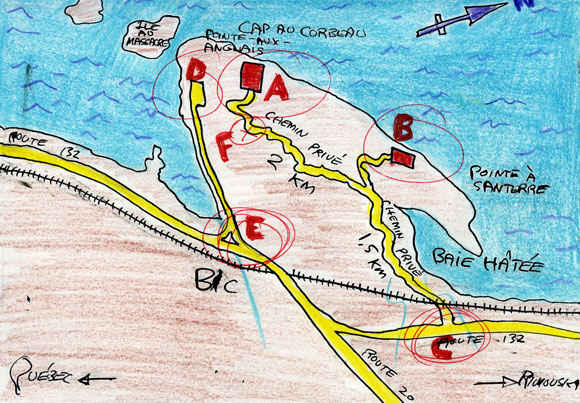
\includegraphics[height=80mm]{corps/chapitre18/img/carte.jpg}
%\end{floatingfigure}

Robespierre a vite fait d’installer sa panoplie du petit généralissime dans le salon et, minutieux, il se met en devoir de réarticuler tous les détails de son plan d’intervention. Le commando partira avec deux voitures. Dans la première, celle de Shimoune, les quatre hommes prendront place et, dans la seconde, une auto-patrouille officielle bien identifiée à la Sécu, Marie-Odile sera seule. Shimoune restera sur la 132 jusqu’au Bic, et bifurquera vers la droite à l’intersection menant à la pointe aux Anglais.

- Ici à «E», tape-t-il de sa canne.

Le préposé au Nutrisuz réprime in extremis le besoin de pouffer de rire.

- De là, on parcourt environ un kilomètre et on stationne ici à «D». Y a toujours de la place. On verrouille et on suit Shimoune dans le bois qui nous amène en vue de l’objectif représenté ici par la lettre «A». Pas besoin de machettes, c’est assez dégagé. On demeure embusqué sans grouiller ni parler jusqu’à 14 h. Pendant ce temps, continue le stratège, Marie-Odile quitte la 132 à la Baie-Hâtée, lettre «C», et emprunte un chemin privé. Il n’y a aucune barrière. Elle roule jusqu’à sa position d’attente et n’en bouge pas avant 13 h 58. Personne n’est censé la voir. C’est ici, lettre «F». À 13 h 58, elle redémarre et, à 14 h, elle commence à faire du bordel avec son auto-patrouille devant l’entrée. Normalement les deux gardiens vont s’approcher pour savoir ce que la Sécu vient faire dans leur petit paradis perdu. Jusqu’ici ça va ?

- Ça va ! répond-on en cœur.

- Nous autres, les gars, à précisément 14h, on fonce vers le pavillon et on l’investit.

Shimoune lève la main.

- Y s’passe quoi si Marie-Odile n’est pas arrivée ?

- On va le savoir, on ne l’entendra pas faire son bordel. On va simplement patienter jusqu’à ce qu’elle se pointe le bout du nez. Mais ça ne se produira pas. N’est-ce pas Marie-Odile ?

La femme flic se contente de sourire.

- Le fait de pénétrer dans la maison va attirer l’attention des deux gardes et ils vont faire deux choses. Ils vont courir vers nous pour voir ce qui se passe et, en même temps, ils vont téléphoner à leur supérieur pour annoncer un incident majeur. Pendant ce temps-là, Marie-Odile vient se positionner sur la galerie avant, juste en haut des escaliers, et elle nous attend, Shimoune et moi. C’est nous trois qui protégerons Timothée et Claude. OK ? Shimoune, rappelle-moi ton rôle !

- Je te suis au pas, mon bel Hannibal, et je viens me faire aller les biceps à côté de Marie-Odile sur la galerie avant. Youhou les amis, venez admirer mes formes voluptueuses ! Mais le premier qui se laisse tenter, je lui casse le nez.

- Espèce d’agace ! OK. Et toi, Marie-Odile ?

- Je descends de mon auto et je gagne la galerie où je vous attends, toi et Shimoune. Le premier qui approche, je lui pète les dents.

- Ouille ! Et toi Timothée-Milet Rioux-Tardif ?

- Je te suis dans la cour, j’attends que tu ouvres la porte d’en arrière ou que tu la défonces si on l’a verrouillée, j’entre à mon tour et je fonce vers la droite où je filme tout ce que je vois en mode téléversement actif – c’est la petite lumière bleue qui clignote. Mon objectif ? Les deux Turcotte.

- OK ! Et notre jeune ami, monsieur Sey ?

- Même chose que Timothée, mais moi je fonce vers la gauche. Dites, monsieur Alcide, il arrivera quoi de l’appel à l’aide que feront les agents qui nous verront attaquer le pavillon ?

- L’appel sera reçu directement chez Barrett à cinq minutes d’ici. C’est la lettre «B». Comme c’est le haut lieu des basses œuvres de l’organisation Turcotte, il s’y tient toujours des activités partisanes. Ce qui m’incite à croire qu’il y a, en tout temps, des fiers-à-bras en attente de casse. C’est comme ça que ça marche. J’imagine qu’ils vont venir avec une ou deux voitures, c’est-à-dire avec deux ou quatre gorilles que Marie-Odile, Shimoune et moi devrons neutraliser. Le plus vite qu’ils peuvent arriver c’est cinq minutes après notre petite invasion domiciliaire. Mais cinq minutes c’est amplement suffisamment pour que Timothée et vous, monsieur Sey, puissiez filmer la cible et téléverser vos enregistrements vidéo dans le serveur sécurisé de la Sécu, au Centre. Dès lors, les méchants seront foutus et, s’ils tiennent malgré tout à la bagarre, ils la perdront, n’est-ce pas Marie-Odile, n’est-ce pas Shimoune ? De toute façon, elle sera légalement retenue contre eux. Rassuré, monsieur Sey ?

- B’en, si c’est ce qu’il faut faire pour recommencer à traiter les personnes âgées avec un peu de dignité, à cesser de les considérer comme des animaux indésirables, pour leur ouvrir toutes grandes les fenêtres sur la vie, les jeunes, la nature, le vent du fleuve, la joie de vivre, ma réponse, monsieur Alcide, moi le p’tit cul de 28 ans, c’est que oui, ça va et que je suis fier d’en être.

- Parfait ! Madame, messieurs, il ne nous reste plus qu’à synchroniser nos montres.

Mais depuis un bon moment, Romain est en bas, au pied de l’escalier, et, très inquiet, il essaie de savoir ce qui se trame chez son fils. À sa connaissance, c’est la première fois qu’il s’y trouve autant de monde en même temps. Qui plus est, de jour ! Pour mieux arriver à comprendre, il a même déposé Gazou, manu militari, sur la corniche entre poules et lapin. Sans bouger, il prête l’oreille, soucieux de déchiffrer les bribes de conversation qui lui parviennent. Voilà maintenant que c’est le carillon d’entrée qui se fait entendre, suivi de pas, de paroles vagues, puis encore d‘autres pas qui, cette fois s’approchent de l’escalier. Rapidement, le vieil homme regagne son salon.

C’est Béatrice qui apparaît dans le cadre de la porte. Elle avait effectivement promis la veille de passer visiter Marie en début d’après-midi. Oui elle a eu le loisir de voir les gens qui sont en haut, non elle ne sait pas de quoi ils discutent, bien qu’elle ait remarqué un plan affiché sur un lutrin, et non elle ne les connaît pas tous.

- Y a un blond bizarre avec des bras musclés et un plus jeune, une espèce d’intello pas souriant. Les autres c’est Timothée, notre ami Robespierre Alcide et une agente de sécurité du Centre, Marie-Odile Tremblay.

- Y s’passe quelque chose en haut, ça, c’est sûr.

La Maririou ouvre de grands yeux.

- Voyons Romain, que ch’est que tu veux qui’ch pache ?

Convaincu de devoir insister, Romain présente la synthèse de ce qu’il a perçu, enrichi de ce que Béatrice vient d’ajouter. Cinq personnes réunies chez Timothée sont en train de parler très sérieusement – «y a même un agent de sécurité avec eux» - de s’en aller filmer les parents du gros Turcotte dans leur cachette. Ils savent où aller et ils ont un plan d’attaque.

À l’extérieur, Gazou hurle à la mort, ce qui affole les poules et angoisse les lapins. Sans parler des résidents de la rue. Marie se lève, une étrange lueur dans les yeux, et va faire entrer l’affreuse bête. En apercevant Béatrice, le cabot ravale sa hargne et son hostilité pour aller se prosterner en face d’elle dans le plus mystique des silences.

Le gros Turcotte ! Le pouvoir des colosses aux voix rauques, grasses et tonitruantes, aux mains énormes, velues, tachées de nicotine, encroûtées de malfaisances, des mains animales, primitives, exécutrices qui égorgent les écoles de musique, qui frappent les petites filles de onze ans, qui détruisent les vies, qui institutionnalise l’échec dans la suite des choses.

- T’es chertain que che chont les parents du gros Turcotte ?

- C’est ce que j’ai entendu à quelques reprises.

Si les jeunes, en haut, ont décidé d’agir ainsi, ce n’est probablement pas pour le plaisir de faire de l’exercice. Il faut plutôt imaginer, puisqu’il est question de parents illégalement cachés, que la manœuvre projetée est en rapport avec eux, Romain et Marie, deux vieux trop avancés en âge pour qu’on songe seulement à leur en parler. Timothée veut-il essayer de faire chanter le ministre pour leur négocier une meilleure qualité de vie ? Si cela est possible, le plan, quel qu’il soit, les concerne. Cela ne risque-t-il pas de changer leur vie, en mieux ou en pire ? De toute façon, les choses ne peuvent aller plus mal que maintenant; il faut agir !

- C’est choquant qu’ils ne nous consultent pas, on n’est quand même pas encore rendu gaga !

- On est loin d’être rendu gaga, mon Romain ! S’ils jont trouvé les géniteurs du gros verrat, faut que je chois là, faut que je l’attrape le gros malfaijant, faut que j’lui coupe ches groches pattes épeurantes pour plus qu’il fache plus de mal à perchonne.

Romain se retient de réagir. Il sait que si sa vieille a une idée précise en tête, il n’y a plus rien à faire.

- Comment tu vas faire ça ? risque-t-il.

En trois mots secs, elle explique que s’ils montent au rez-de-chaussée, tous trois, là maintenant, Timothée et sa bande ne voudront jamais les intégrer à leur équipée. À coup sûr, ils vont justifier le danger de l’opération, l’état de santé de Marie, le tour de taille de Romain, la convalescence de Béatrice, voir l’alignement des planètes rendant impossible toute mission de plus de cinq exécutants. Il faut donc trouver une façon de participer à la fête sans attendre d’être invités.

- On écoute che qui che pache en haut et quand on les jentend partir, on che dépêche et on les chuit dans le char à Béatriche. T’as-tu un meilleur plan ?

Romain bouge la tête à l’horizontale et regarde Béatrice qui hausse les épaules en souriant.

- Bon ! J’m’en vas me préparer.

Cinq minutes plus tard, elle ressort de sa chambre en robe fleurie jaune, verte, noire et blanche, avec collants gris et souliers vernis, toute coiffée comme pour la messe de minuit, tenant, dans sa main gauche, un parapluie. Constatant les regards dubitatifs sur son accessoire conçu davantage pour le crachin atlantique que pour les chaudes après-midi de juillet, elle leur en donne l’explication.

- Perchonne au monde ne bloque le chemin à une p’tite vieille qui a l’air de chavoir manier un parapluie.

Suit alors une courte période d’attente qui se termine par un branle-bas de combat au-dessus de leurs têtes.

- Cha y est !

Ils perçoivent clairement une voix de femme s’écrier qu’elle va suivre avec sa voiture. Suivre qui ? Sûrement Timothée et les autres gamins. Plus une seconde à perdre ! Béatrice et Romain commencent à monter tandis que Marie ferme la porte au nez de Gazou, «Moman part pas longtemps, chois gentil !», lequel, aussi con qu’un pot de beurre d’arachides, se remet à hurler comme si la fin du monde était arrivée. La contemplation de Béatrice entraînerait-elle un état de dépendance et son manque, une souffrance intolérable ?

- Envoye, Romain, t’as donc b’en d’la misére à grimper les marches !

- J’ai p’us vingt ans !

Béatrice se précipite vers la porte.

- Dépêchez-vous, elle vient de décoller.

En ahanant, Romain parvient à l’auto où la Maririou est en train de s’attacher sur le siège avant. Il a à peine le loisir de s’asseoir que déjà, Béatrice a embrayé et que l’hybride chinoise fonce en direction ouest. Rue La Salle, elle entrevoit, au loin, le véhicule de la Sécu qui vient d’arrêter au feu rouge du boulevard Saint-Germain.

- On l’a rattrapée !

Le reste de la filature est sans histoire. Trois cents mètres prudemment en arrière, Béatrice a le temps d’apercevoir Marie-Odile quitter la 132 à la Baie-Hâtée. Comme on ignore où ce chemin privé mène, le mieux, estime Romain, est de l’emprunter et de voir. Au pire, l’agente de sécurité les remarquera et viendra les houspiller. Au mieux, ils la suivront, invisibles, jusqu’à sa destination.

Peu après, ils passent devant une ramification secondaire qui semble conduire à une propriété cossue dont on entraperçoit quelques détails évanescents au travers les arbres. Dans le pare-brise, la petite route en gravelle serpente cahin-caha et bloque toute perspective de plus de 100 mètres, tant et si bien que la conductrice doit redoubler de prudence pour ne pas être repérée.

Après cinq ou six minutes de reptation à bas régime, l’infirmière aperçoit, de loin, ce qui pourrait être la voiture de la Sécu immobilisée et elle ferme son moteur. Son rythme cardiaque a augmenté de façon perceptible.

- Qu’est-ce qu’on fait si elle fait demi-tour ?

- On a l’air fou, ronchonne Romain. Mais on dirait qu’elle attend quelqu’un ou quelque chose.

- Je vais aller voir. Vous autres, restez pas dans l’auto. Si jamais quelqu’un vient…

Doucement, on ouvre les portières et on entre dans le sous-bois. Avec toutes les ruses expérimentées au fil des millénaires par l’ensemble des peuplades amérindiennes, les vieux marchent jusqu’à la carcasse d’un tremble recouvert de mousse et Béatrice s’avance en direction de Marie-Odile. Sans faire craquer de branches, elle réussit à s’en approcher à dix mètres où, immobile, elle épie. Rien ne bouge, personne ne vient. Seuls les oiseaux font preuve de vie. Puis, comme si elle obéissait à une consigne, l’agente de sécurité démarre en trombe et disparaît dans les courbes prononcées du chemin. L’infirmière a beau s’étirer, elle ne la voit plus. Hésitant sur la marche à suivre, elle choisit de s’en retourner vers sa propre voiture, mais, chemin faisant, elle entend le moteur de Marie-Odile s’arrêter, une portière claquer et une voix féminine crier des choses qu’elle n’arrive pas à bien comprendre. Elle refait volte-face et continue sa progression dans la lourde couverture boisée. Elle a vite fait de repérer une clairière où elle aperçoit l’auto-patrouille, puis l’agente de sécurité en train de courir vers une grande maison, tandis que deux gaillards, on dirait des gardiens, se hâtent, eux aussi, vers l’arrière de la propriété, la main sur leur système personnel de communication. L’un d’eux invective lourdement la policière, utilisant des termes blessants, l’autre ne cesse de parler dans son appareil. Puis tous deux changent de cap et s’avancent vers Marie-Odile qui, en position dite du «sablier large», le Hangetsu-Dachi, les attend silencieusement en haut des marches de la galerie. La perspective de recevoir des coups les fait hésiter et ils tentent de parlementer. C’est alors que Robespierre et son copain, le gars aux bras surdéveloppés, apparaissent à leur tour; ils étaient dans la maison. Prudemment, les deux gardiens font machine arrière ce qui incite le blond à adopter la pose de Monsieur Univers et à s’agiter la musculature.

- Hé ! les tites filles, dites-moi pas qu’on vous fait peur !

L’un des gardiens lui signifie un doigt d’honneur.

- On a “câllé” du renfort, t’es faite le fif, toi aussi la Bitch !

Ce que Béatrice comprend, c’est qu’une partie de ceux qu’elle a vus tout à l’heure sur la rue Crouet est ici en train de braver des gardiens de sécurité qui ont appelé du monde à la rescousse. Elle ignore où sont les deux autres, Timothée et l’intello, mais elle sait que des gens s’en viennent, possiblement des taupins mal intentionnés, des gens qui vont obligatoirement emprunter le chemin où est approximativement garée sa voiture et près de laquelle patientent présentement deux vieillards. Convaincue du pire, elle saute sur la gravelle et se met à courir en leur direction.

- Restez cachés, leur crie-t-elle tandis qu’elle met le contact pour se stationner sur l’accotement, un bien grand mot pour qualifier la roche grossière mal râtelée de chaque côté du chemin.

Satisfaite de voir ses portières de droite empêtrées dans les premières branches, elle verrouille et se fond dans la verdure où elle vient rejoindre ses compagnons. Malheureusement, elle doit retourner à l’auto, Marie tient absolument à son ombrelle, ce qu’elle fait sans maugréer.

Pendant qu’elle leur raconte tout ce qu’elle a vu au pavillon, des bruits de moteur se font entendre. Tous trois se tapissent et assistent au passage à vive allure de deux voitures trimbalant chacune, quatre casseurs. Aucun ne semble porter attention à l’hybride de Béatrice.

- Ces gars-là, madame Rioux, ils s’en vont à la maison, là-bas, ramasser Timothée et ses amis.

- Là où che cachent les parents du gros Turcotte ?

- Oui.

- J’ignore quelle idée ils jont eue Timothée et ches amis, mais là, che que je vois, c’est qu’ils vont che faire rentrer dedans. Cha va faire ! Je m’en occupe ! En route !

Et la Maririou de quitter le sous-bois pour s’en retourner prendre place dans l’auto.

- Dépêche, crie-t-elle à Béatrice.

- Voyons madame Rioux, ça n’a pas de bons sens ce que vous voulez faire là !

- Vite, gronde Romain en se hâtant à son tour vers le véhicule, fais ce qu’a te dit, elle sait ce qu’elle fait !
Mais au même moment, les choses se gâtent au pavillon. Aux deux gardiens se sont ajoutés huit videurs armés de matraques et possiblement d’armes à feu, qui s’approchent de la galerie où Robespierre, Marie-Odile et Shimoune jouent les matamores. De l’intérieur, la voix de Timothée se fait entendre :

- C’est beau, Robespierre, on a tout. Mission accomplie !

\begin{floatingfigure}[l]{45mm}
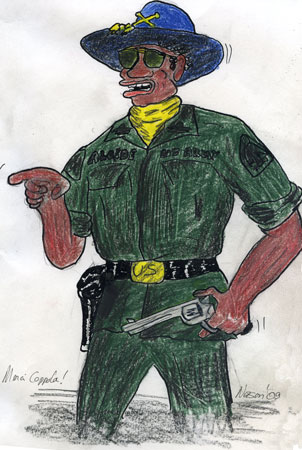
\includegraphics[height=60mm]{corps/chapitre18/img/personnage-robespierre-colonel.jpg}
\end{floatingfigure}

Le colonel Alcide sourit ! Jusqu’ici, sa stratégie a fonctionné. Sauf que, devant lui, la perspective est moins enthousiasmante. Il va maintenant falloir en découdre avec deux fois plus de salopards que prévu.

C’est Marie-Odile qui se lance dans les frais, une improvisation par rapport au plan initial, une improvisation heureuse.

- Écoutez-moi bien, gang de bolos. Nos gars en dedans ont filmé tout ce qu’ils étaient venus filmer et ils en ont téléversé une copie dans le serveur de la Sécu au Centre. Nous avons maintenant toutes les preuves que nous voulions. Pour détruire ces documents, ça va prendre un ordre de la Cour. À c’t heure, vous avez le choix. Vous venez nous chercher ou vous nous laissez filer sans violence.

Un peu en retrait des autres, un des sbires de Pete Barrett ne cesse de parler dans sa boucle d’oreille, ce qu’il fait avec force gestes sans trop s’occuper de ses collègues qui eux, semblent plutôt décidés à déloger les occupants de la galerie.

- Tout ce que vous faites présentement est filmé et archivé, continue la femme flic en pointant sur le premier bouton de sa chemise. Utilisez vos guns et vous serez poursuivis pour tentative d’homicide.

- Ta gueule, astie de Bitch, crie un des malabars. Let’s go, les boys, on les défonce !

Et les affreux de se mettre en branle. L’intensité est à couper au couteau. Dans quelques secondes, les coups vont pleuvoir. C’est précisément à ce moment qu’arrive, à file épouvante, la voiture de Béatrice, laquelle vient de franchir sur les chapeaux de roues trois croches et une montée à pic. Sans hésiter, la Maririou en descend et, pointant du riflard, fonce de son pas précipité de petite vieille pas commode vers le pavillon. Il faut la voir se faufiler au milieu des malfrats en les tassant avec son improbable accessoire. La stupéfaction est totale. Personne ne la connaît, personne ne l’a jamais vue, ni les méchants qui n’osent se placer sur son chemin, ni le trio en position défensive sur la galerie qui la laisse monter. Mais c’est Romain qui est encore le plus impressionné. Il sait parfaitement bien que toute sa vie, sa belle Marie a eu peur des hommes violents et la voilà en train de les bousculer à la manière de volailles dans un poulailler.

- Bonjour madame, à qui ai-je l’honneur ? lui demande Robespierre.

- Laiche faire les jonneurs, toi ! Ouvre-moi la porte !

Et elle s’introduit dans le pavillon.

Dans sa foulée, Romain et Béatrice tentent d’avancer. Mais deux gredins ont tôt fait de les intercepter, un peu comme s’il était hors de question qu’on leur refasse le coup de la vieille dame au parapluie.

Ce que voyant, Marie-Odile hurle de plus belle.

- Tout est filmé !

Intimidé, le gorille qui retient Romain le relâche aussitôt, mais son collègue hésite à en faire autant avec Béatrice. Distrait dans son incertitude, il ne voit pas venir le coup de genou dans ses parties normalement intimes. C’est en geignant qu’il entend cette belle fille rajouter une kyrielle de grasses insultes à sa sourde douleur et qu’il la voit prendre la main du vieillard pour l’amener en direction de l’immeuble. Sur la galerie Marie-Odile a presque souri.
Aussitôt entrée, la Maririou remarque Timothée qui vient vers elle, la regardant incrédule, comme s’il eut vu apparaître Bea Bellow armée d’un lance-roquettes. Puis, juste à côté, elle aperçoit la personne qu’elle cherchait, une forte femme d’allure austère qui semble très contrariée par la situation générale.

- Mimi Turcotte, t’es pas chensée être morte il y a quatre ans, toi ?

- P’is toi, Marie Rioux, t’es pas censé l’être depuis six ?

Toutes deux se dévisagent comme si elles s’accusaient d’avoir raté un soufflé.

Derrière la mère Turcotte, quelques vieillards se sont approchés dont son époux Jean-Pierre, une montagne de chair vaguement connue de Romain, Romain dont les yeux haineux fixent ces illégaux financés par la princesse, ces vernis torchés blanchis par le pouvoir libéral, ces planqués aux panses replètes gavées par les contribuables. Et il explose. Voilà six ans que lui et sa compagne sont enfermés dans un sous-sol qui sent la crasse en raison d’une loi inique que le fils Turcotte a fait voter et a mise en place. Et pendant ce temps-là, pendant qu’il faisait crever des milliers d’aînés dans des CRG mal équipés, pendant qu’il en condamnait un plus grand nombre à la clandestinité, à la non-existence officielle, à la peur, aux privations, aux abus de toutes sortes et aux souffrances, une petite clique de gras dur, son père et sa mère en tête, menaient un train d’enfer propre aux parasites institutionnalisés.

- Romain, arrête !

Ce cri venu du fond des tripes est accompagné par un violent coup de riflard sur la table de la salle à manger. Un vase de fleurs des champs se renverse.

- Ch’est mon affaire. Ch’est moi qu’il a trahie le gros crevard. Toi, il ne t’a fait que chouffrir, comme tous les autres vieux du Québec. Mais moi, en plus et churtout, il m’a abujée.

Mimi Turcotte est effarée et l’obèse à ses côtés n’ose parler.

- Mais avant que tu m’entendes, Mimi Turcotte, tu vas chortir dehors et tu vas dire à tes chiens de retourner dans leur cabane. Je te tiens rechponsable des coups qui vont ch’échanger.

Étrangement, la mégère évite de répondre et gagne la galerie où elle lève les deux bras.

- Arrêtez tout, crie-t-elle aux tueurs. J’ai le contrôle; attendez les ordres de Pete avant de bouger.

Aussitôt dit, aussitôt fait. Les casseurs se replient jusqu’au chemin d’accès, leur chef en grands pourparlers téléphoniques.

Robespierre qui vient de voir son plan complètement bousillé, heureusement bousillé, s’approche de Marie.

- Mon ami Timothée me dit que vous êtes sa mère, madame. Je suis très heureux de vous connaître. Mais venez vous asseoir ici à la table. Faut plus vous en faire, on a le contrôle. On a tout filmé. On a ramassé assez de preuves pour faire dégommer le gros pourri et pour initier un grand ménage au Centre.

Claude Sey semble ravi.

- Pauvre ‘tit garchon, qu’elle répond à l’armoire à glace chocolatée - étrangement, elle n’en ressent aucune crainte - en se laissant conduire jusqu’à la table. Y a quelque chose que t’as pas compris.

Toute sa vie, crache la Maririou, elle s’est réfugiée dans la musique, totalement, hermétiquement, cela pour se créer un univers où les Edmond Rioux ne pouvaient accéder. Elle a cru pouvoir y arriver et a même essayé d’expliquer la méthode à des enfants qui, comme elle, avaient été victimes d’hommes en situation de pouvoir, des agresseurs, batteurs, forts en gueule, gueulards à voix tonitruantes, ivrognes colériques, manipulateurs, violeurs et autres monstres, des hommes terribles à l’origine d’existences impossibles à raccommoder et de petites filles de onze ans perdues à tout jamais. Or, dans cette lignée de misérables, Sylvain Turcotte venait prendre place assez haut dans l’échelle d’infamie. Au lieu de respecter sa parole dans l’histoire de l’École de musique, il avait laissé tomber l’institution quinquagénaire comme s’il eut été question d’un insignifiant projet d’été. Pourtant, il s’était bel et bien engagé auprès d’elle, Marie Rioux. Il avait juré de sortir l’École des difficultés financières qui l’accablaient. Malgré cela, il avait agi en sens contraire, ce qui ne l’avait surtout pas empêché de devenir par la suite encore plus puissant, plus gros, plus épeurant, comme, naguère, Edmond Rioux qui, chaque fois qu’il revenait à la maison et qu’il la battait, lui semblait plus terrifiant que jamais. C’est connu, les salauds grandissent dans l’ignominie. Dans l’esprit de la vieille violoncelliste, son père, cet être détesté qu’elle continue aujourd’hui de craindre dans ses cauchemars, lui a tué sa vie, et Sylvain Turcotte, l’homme fort de Rimouski, qu’elle hait dans une rigueur dénuée d’émotions, lui a tué son projet de vie. Ce sont deux exemples de ce pouvoir anéantissant qui vient, parfois, frapper les petites filles de onze ans, même si elles sont devenues des septuagénaires avancées.

- T’auras beau le faire dégommer, le gros verrat, il va rechter méchant, dangereux, épeurant. T’as-tu compris qu’il fallait lui arracher les dents, lui couper les mains, lui nouer la queue, le rendre dochile comme un chien de perron. Tu pourras alors lui donner des coups de pieds et il pourra pas te mordre !

Le docteur Robespierre qui discerne toute la souffrance de cette vieille vie, se garde bien de répondre. Seule Mimi Turcotte s’essaie.

- Tu trouves pas que tu exagères un peu beaucoup, Marie Rioux ! Ta vie a été une catastrophe et tu veux te venger sur mon garçon !

Béatrice s’est rapprochée et s’est assise sur la chaise voisine de Marie. Par réflexe nerveux, elle lui caresse un instant l’épaule.

- Qui t’a parlé de vengeance ? Pour che venger, il faut être enragée. Moi, Mimi, j’chuis calme. Chereine, même. Je parle cheulement d’administrer une prochédure comme quand on opère une bête puante pour qu’elle ne nous arroje plus ou un cherpent pour qu’il ne nous empoijonne plus. Je vas faire cha pour me faire du bien. Au moins une fois dans ma chienne de vie ! Avant qu’il choit trop tard !

Marceline non plus n’avait pas opéré dans la rage, la vengeance ou l’émotion. Elle avait frappé un animal dangereux qui menaçait sa petite fille de onze ans. Pour la protéger. Pour éviter plus de mal. Pour l’avenir, pas pour le passé.

La suite est inattendue. Tout d’abord, Shimoune vient parler dans le creux de l’oreille de Robespierre. Puis il revient avec un des hommes de Pete Barrett qui, sans une parole, prête sa boucle d’oreille à Mimi Turcotte. L’instant est dramatique. Quelques moments plus tard, l’organisatrice libérale met fin à la communication et regarde Marie.

- T’as gagné ! Pete veut négocier !

Des exclamations de joie fusent ici et là, Claude Sey au bord des larmes et Timothée lourdement silencieux, comme s’il ravalait des litres et des litres de peine contenue. Marie-Odile assène un amical coup de coude dans les côtes de Shimoune. Le colonel Alcide n’a pas le temps de parler que déjà, la générale Rioux a donné ses ordres.

- Avant de négochier, Mimi, tu vas renvoyer chez eux les méchants qui chont dehors et tu vas me garantir qu’on peut tous repartir d’ichi chans que rien ne nous arrive. Rendus chez nous, on va regarder cha et on va te contacter.

Une heure et demie plus tard, Marie et Romain participent à ce qui leur avait été interdit depuis l’été 2027. Assis dans le salon de Timothée, ils boivent du vin et mangent de la pizza en compagnie d’étrangers, des hommes et des femmes ivres de joie et de tension dissipée qui n’ont de cesse de se relayer pour se rappeler les grands moments de l’après-midi.

- Mesdames, messieurs, s’écrie Robespierre.

Le silence se fait.

- Je propose un toast à notre chef, à celle qui a rendu possible cette victoire sans qu’il n’y ait d’égratignure, à quelqu’un que j’ai été fier de rencontrer aujourd’hui, à madame Rioux !

Un concert de bravos et d’applaudissements suit.

Après, lentement, comme si on voulait s’accrocher au plaisir d’être dans le groupe, le commando se démobilise, tout un chacun regagnant son domicile. C’est Marie-Odile qui va offrir à Robespierre de le reconduire à sa voiture dans le stationnement du Centre.

- Faut que j’aille porter l’auto-patrouille.

Timothée sourit et les accompagne à l’extérieur.

- Hé-hé-hé, qu’il fait à son ami.

- Quoi «hé-hé-hé» ?

- Juste «hé-hé-hé».

La brunante est déjà avancée et, pour la énième soirée consécutive, le vent est doux et parfumé. Devant sa maison, près du cimetière, un lampadaire commence à décorer la rue de ses effets de lumière et, sous son halo, Béatrice, sortie tout à l’heure humer l’air des terres, semble attendre un signe de la vie. Béatrice, la fille de la lanterne. Attiré comme un papillon de nuit, Timothée s’approche, atrocement gêné malgré ses trois verres de vin. Quand bien même il tenterait de parler, de dire ce que doit en de telles circonstances, il n’y arriverait pas. Rien ne sortirait et, de toute façon, il ne saurait trouver les mots.

C’est ce qui explique qu’elle lui prend la main.

- Dis rien, Timothée, dis rien, je sais que tu es bon. Reste avec moi.

Maladroitement, il prend place à côté d’elle sous le lampadaire, paradis dont les anges pardonnent les bedondaines, les barniques et les chauvaisons.

    So woll’n wir uns da wieder seh’n
    Bei der Laterne wollen wir steh’n
    Wie einst Lili Marleen
    Wie einst Lili Marleen
    (C’est dans ce coin-là que le soir
    On s’attendait près de la lanterne remplis d’espoir
    Tous deux, Lily Marlène.
    Tous deux, Lily Marlène.)


\chapitre{Lyre de lumière et de liberté, le lundi 10 juillet 2034 }{Erigé au début des années 70,}{ le complexe gouvernemental de Rimouski conservait son austérité d’origine, une froide sobriété tout de béton vieilli et de bois trop pâle pour faire s’épancher les cœurs, cela, malgré les rénovations auxquelles on l’avait soumis en 60 ans de services paperassiers. Au sous-sol, dans ce qui avait naguère servi de bureau régional pour le ministère de la Culture, on trouvait aujourd’hui une salle d’audience, véritable petit tribunal avec tout le décorum : drapeau du Québec, photos du premier ministre et de Sylvain Turcotte, vieux cadres numériques faisant défiler leurs scènes rupestres, forestières et maritimes, sans oublier une horloge et un calendrier électronique. On y avait entendu des promoteurs sur des histoires de prolongements routiers, des écologistes sur des questions d’enfouissement, des pêcheurs sur des enjeux de surpêche. }

Mais depuis trois mois, les locaux étaient utilisés par la Commission de réinsertion civile des victimes de la loi 173 de 2028, alias la CRC, une structure sans appel mise en place pour gommer certaines injustices survenues dans l’application de la législation Turcotte. 

Dans le cadre de la contre-réforme enclenchée dans les semaines qui avaient suivi les événements de juillet 2033, Québec avait reconnu, sur la proposition même du ministre Turcotte - une position politique déroutante que seuls quelques Rimouskois savaient forcée, le couteau sur la gorge - que certains illégaux avaient été contraints de le devenir par crainte justifiée du Bureau des affaires gérontologiques (BAG), structure policière honnie dont le démantèlement avait été terminé en janvier dernier. Ainsi, plusieurs centaines de vieillards officiellement déclarés morts avaient choisi de quitter la clandestinité pour venir plaider en faveur de leur «résurrection civile». Il leur suffisait de démontrer qu’ils n’avaient eu d’autre choix que de se cacher, traqués injustement par le BAG à la suite d’une obscure délation ou d’un discutable contrôle fiscal, la CRC leur donnait habituellement raison. À plus forte raison, que l’enquête publique du coroner actuellement en cours sur les liens pouvant exister entre chocs anaphylactiques et Nutrisuz, battait son plein avec l’attention des médias d’un peu partout, incluant ceux de la Nouvelle-Zélande et de la Suède. Et plus le temps passait, plus l’horrible soupane était décriée et pointée du doigt comme étant la cause de nombreux problèmes de santé. On s’attendait même à un recours collectif monstre dès le dépôt des conclusions à la suite des audiences. Le titre de Monsanto avait connu une chute historique.

À l’inverse, la CRC rejetait parfois les prétentions de certains demandeurs, des cas vraiment trop sulfureux pour être banalisés. Ces gens étaient alors accusés de fraude et confiés au criminel. C’est possiblement ce qui aurait pu arriver aux parents, père, mère, oncles et tantes, du gros Turcotte. Pour éviter qu’ils soient cloués au pilori et livrés à la vindicte populaire, il avait été convenu de part et d’autre, au lendemain des événements, d’offrir à ces profiteurs une nouvelle identité légale et d’en faire des résidents anonymes d’un CRG montréalais. Il ne pouvait être question de les installer dans celui de Rimouski en raison, notamment, du projet visant à le convertir en vraie maison de retraite, au grand dam de Carl Michaud, rétrogradé au rang de gérant et contrôlé dans ses moindres faits et gestes. Pour tout dire, le cadre supérieur au panache si impressionnant n’était plus que l’ombre de lui-même. En le voyant, on aurait dit un petit quincaillier en train de liquider sa faillite.

De part et d’autre ? C’est une des mesures qui avaient été négociées entre le commando dont Marie avait pris le contrôle et les gens de Sylvain Turcotte qui, sous leurs pieds, sentaient le vide sinistre de l’échafaud.

\begin{floatingfigure}[l]{45mm}
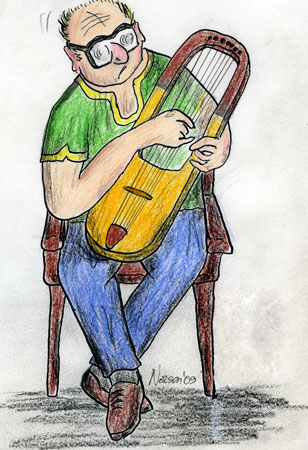
\includegraphics[height=60mm]{corps/chapitre19/img/personnage-timothee-lyre.jpg}
\end{floatingfigure}

Aujourd’hui, la salle est presque pleine. Au premier rang, Marie Rioux, Romain Tardif et leur conseiller, Robespierre Alcide. Derrière eux, le clan qu’ils ont tricoté à triple laine depuis cette fin juillet de 2033: Timothée, Béatrice, Shimoune Saint-Pierre, Ophélie Marcotte, Claude Sey qui est venu expressément de Montréal, Marie-Odile Tremblay, David Gagnon-Tropecolo, alias le Chinois, ainsi que le docteur Bellavance, Bea Bellow, Louise Lavoie, Sébastien Larose, Jipé Gendron, alias Tit-mononk, Solange Gadoury et Jawad Kebbaj, lequel, pour une fois, ne travaille pas. On remarque également quelques anciens méchants dont les frères Côté, mieux connus sous le sobriquet de Papyblues, Vlado Marcovsky, l’homme de l’informatique, et le bonhomme Jean qui avait particulièrement apprécié être libéré du sous-sol par Timothée lui-même. À un point tel qu’il lui avait «remonté» une Saguewanish grand luxe avec plus d’électronique incorporée qu’il ne s’en trouve au siège social d’IBM et avec un gyroscope dernier cri prévenant toute possibilité de chute ou de perte de contrôle gravitationnel. Une sorte de Dodge Challenger 70 avec moteur stock.

En avant, le commissaire Rémi Anglehart, celui-là même qui assumait la présidence du Centre régional gériatrique avant qu’il ne soit transformé, à la liesse générale, en résidence pour aînés, est en train de lire les considérants et s’apprête à rendre la décision ayant fait consensus auprès des membres de la CRC. La Maririou arbore son visage de pierre et celui de Romain reflète une certaine nervosité. Quant à Robespierre, psychologue officieux, colonel à la retraite et avocat autoproclamé, il sourit pour cacher son stress.

- En conclusion, la Commission est d’avis que malgré l’illégalité de l’ensemble des gestes posés, vous avez eu raison, «ab initio», de vous soustraire aux efforts des agents du Bureau des affaires gérontologiques. Leur eussiez-vous obéi, vous auriez été victimes d’une injustice encore plus grave. «Adversus periculum naturalis ratio permittit se defendere».

Anglehart se dérhume. Dans sa tête, c’est en étalant son latin qu’il arrive à se livrer à des effets de toge alors que l’instance qu’il préside n’en requiert aucune.

- En outre, poursuit-il comme s’il était à la Cour suprême, la Commission blâme le gouvernement du Québec de vous avoir contraints à l’illégalité, vous privant ainsi des services auxquels vous aviez droit, ainsi que de tous vos revenus de retraite. Il est donc de mon devoir d’invoquer un «nolle prosequi», de vous déclarer officiellement réinsérés civilement et de recommander au lieutenant-gouverneur en conseil de vous rembourser les prestations qui ne vous ont pas été versées depuis 2028, année où l’on vous a inscrits comme décédés à l’état civil, incluant, «mutatis mutandis», les intérêts que la Commission a établis à 8,367 %.

Les premiers cris de joie se font entendre.

- À l’ordre ! À l’ordre !

C’est peine perdue. Des gens accourent pour féliciter Marie, Romain et Robespierre. Le commissaire doit hausser le ton.

- Ladite Commission, crie-t-il littéralement, fera publier, d’ici dix jours, un avis dans tous les médias du Bas-Saint-Laurent à l’effet que vous, Marie Rioux et vous Romain Tardif, autrefois de Saint-Anaclet, maintenant du quartier Nazareth de Rimouski, avez, entre 2028 et 2034, agi «bona fide», que vous avez été réinsérés aux dépens de l’État, que vous avez bel et bien été victimes d’une loi mal appliquée et, «res ipsa loquitur», que vous recevrez les excuses formelles du gouvernement du Québec.

À ces mots, la salle explose comme à un match de football. Anglehart n’a jamais rien vu de tel. Claude Sey a les larmes aux yeux, Tropecolo lui serre les deux épaules de ses courtes paluches, Jawad Kebbaj donne l’accolade à Timothée, Ophélie fait la bise à Shimoune, Bea Bellow sourit et, l’espace de deux secondes, frotte ses jointures de la main droite sur l’avant-bras de Robespierre, imitée par Louise Lavoie qui elle, embrasse carrément le colosse sur la joue, ce qu’observe Marie-Odile, la nouvelle responsable de la sécurité, qui lorgne la scène du coin de l’œil par crainte inavouable qu’on lui pique l’homme de sa vie, son beau Robie. Au même moment, Tit-mononk lève un spectaculaire bras d’honneur en direction de la photo du premier ministre sous les rires de Marcovsky et sous la mine ravie, celle des grands jours, de Sébastien Larose qui venait tout juste de prendre sa retraite. Le père Jean, lui, file sur la Saguewanish Hot Rod prétextant un dernier ajustement. Quant au docteur Bellavance, homme de science auquel plus personne n’accole l’épithète de «sinistre», il gagne discrètement la sortie, un sourire accroché au visage, suivi de Solange Gadoury qui semble ne plus vouloir le quitter depuis qu’il mène un projet de reconditionnement nutritionnel destiné aux cas de patients ayant développé une intolérance pathologique à la nourriture en raison des abus de Nutrisuz. Jamais sa vie n’a été aussi intéressante.

À son tour, l’arrière-petit-fils de l’inventeur du Pétépano s’approche de Marie.

- On les a eus, madame Rioux ! Et dans l’honneur ! Ils vont même vous faire des excuses publiques. Vous allez pouvoir marcher en plein jour, dans les rues de Rimouski, au su et au vu de tout le monde. Vous avez réussi à faire travailler notre matériel, nos preuves. Avec ça, ils ont tous plié. Ils vous ont donné tout ce que vous exigiez.

- Voyons, mon garçon, tu sais aussi bien que moi que dans cette histoire, je n’ai joué que ma partition et que chacun a joué la sienne. Sinon, ça n’aurait pu fonctionner.

Robespierre Alcide qui a tous les talents avec les dames, lui fait alors une profonde révérence.

- Et si on n’avait pas eu une bonne chef d’orchestre, ça n’aurait pas pu fonctionner non plus !

Le lendemain de l’opération commando, Marie avait effectivement exigé la présence de Sylvain Turcotte dans son salon, au sous-sol de la rue Crouet. Louis-Marc Richard n’en était pas revenu de voir autant de voitures, dont celle du ministre rimouskois, arriver chez son voisin d’en face, ce «pas d’allure» hautement suspect. C’est avec la plus tordue des fiertés, qu’une Maririoux aussi rigide qu’implacable avec reçu le haut personnage, assise dans son fauteuil crevé, laissant Gazou essayer de mordre les mollets libéraux qui s’aventuraient trop près de sa méchante gueule. La vieille dame avait exigé la présence de Romain, Timothée, Shimoune et Robespierre et, en contrepartie, avait accepté que quatre sbires accompagnent l’homme politique. D’entrée de jeu, elle avait voulu comprendre pourquoi le politicien avait fait basculer sa famille dans l’illégalité. N’avait-il pas les moyens, lui, «un gros ministre pesant», de subvenir aux besoins de son père et de sa mère pour leur éviter, en toute légalité, l’internement dans un CRG ?

La réponse ne l’avait pas ébranlée du tout. Quand il avait vendu sa terre pour prendre sa retraite en 2028, l’année du référendum, le gros Jean-Pierre Turcotte n’avait, en réalité, que poussé des feuilles de papier. Hypothéquée jusqu’au trognon, la propriété agricole ne lui avait presque rien retourné en équité. Lui-même criblé de dettes, le cultivateur rimouskois s’était retrouvé sans le sou, avec Mimi qui s’assurait, sur une base quotidienne, que la vie soit vraiment invivable. Pour tous revenus, le couple disposait de la pension fédérale et de l’allocation provinciale, celle de la Régie des rentes. De plus, Sylvain leur avançait quelques centaines de dollars tous les mois, la plupart du temps pour payer le loyer de leur 4 ½, rue Saint-Jean-Baptiste. En échange, ils l’aidèrent sérieusement, tous les deux, dans sa campagne référendaire.

Une fois la loi 173 adoptée, les deux Turcotte auraient dû, techniquement, être forcés d’aller habiter au CRG-BSL. C’est à ce moment que Mimi eut l’idée de faire construire un pavillon au Bic et de disparaître avec Jean-Pierre pour mieux s’y cacher. Elle en profita pour offrir cette chance unique à ses deux sœurs et à leurs époux. Sylvain Turcotte fit le nécessaire à la satisfaction générale. D’où le terrible accident de juin 2029.

- Faut me comprendre, ma’me Rioux, j’ai une famille à m’occuper ! P’is une paye de ministre, ce n’est pas une paye de président de compagnie. C’est pas assez pour faire vivre mes parents en même temps que ma femme et mes enfants; j’en ai deux au cégep et un à l’université. Ma femme, vous l’avez connue dans l’temps, elle a pas changé, elle est malade tout le temps, elle travaille pas, elle rapporte rien, c’est toute moi qui paye toute, tout le temps.

La vieillarde avait alors frappé l’accoudoir de son fauteuil, ce qui avait momentanément calmé Gazou.

- Cha va faire, j’en ai achez entendu; tu me feras pas brailler chur ton chort, mon ‘tit garchon. T’es «quelqu’un de pouvoir» qui m’a trahie !

C’est à ce moment que la Maririou, le visage intraitable, avait placé ses cartes : voici les preuves de corruption, voici des preuves de faux déposés au Conseil d’administration, voici des preuves vidéo où le ministre des CRG cache des illégaux, en l’occurrence sa parenté, et voici des preuves démontrant, hors de tout doute, que des vieillards sont maltraités et emprisonnés. Tout ce petit matériel a été stocké dans différents systèmes informatiques pour éviter qu’il ne soit détruit. La seule façon qu’il y reste verrouillé à quadruple tour, qu’il ne soit ni envoyé aux médias, ni remis à la police, ni téléversé dans le quanticordi de Thierry-Ian Dennis-Dubeau, le chef de l’opposition à Québec, c’est que l’on procède rapidement à quelques petits changements.

Petits changements ! Quel euphémisme !

- Mon ‘tit garchon, j’te donne un an pour faire tout che que je vais te demander. Chi tu y arrives pas, t’es dans la misére !

- Ma’me Rioux …

- Pour t’aider, avait-elle coupé, je l’ai tout écrit ichi sur che document. Y en a une copie pour toi et une pour moi que tu vas chigner. Si tu chignes pas, demain matin neuf heures, les médias, la poliche et Dennis-Dubeau, tu chais, Ti-Dédé, b’en ils vont rechevoir toutes les preuves. J’ai quelqu’un qui m’a toute arrangé cha pour que cha parte.

- Ma’me Rioux, ma’me Rioux, vous savez bien que c’est pas comme ça que ça marche. Va b’en falloir que je prenne le temps d’étudier vos demandes. Après, on se rencontrera et on verra ce qui peut être fait.

- Ch’est comme tu veux. Chi tu chignes le papier, tu gardes ta job, chi tu chignes pas, demain matin neuf heures, t’es dans la pire misére noire de toute ta vie ! Y a rien à négochier, abcholument rien, mon pauv’tit garchon ! T’as été malhonnête, tu t’es fait pogner, à ch’t heure, tu paies. À ma fachon ! Chinon, ch’est la prijon, le déjhonneur, le pipi dans les claques.

Bluffeur notoire, Turcotte avait alors fait mine de sortir, les trois janissaires à sa suite. C’est à ce moment que Robespierre avait mis en marche son vieux fond Alcide.

- Êtes-vous au courant, monsieur Turcotte, de la situation sordide dans nos prisons depuis qu’il y a quatre ans, votre régime a sabré de 40 % dans les budgets correctionnels ? Les autres détenus vont tellement vous tabasser que je n’aurai pas besoin d’aller vous porter de caramels, vous n’aurez plus de dents pour les manger et vos lèvres seront des enflures crevassées, des horreurs indicibles.

- Et, avait ajouté le malicieux Shimoune, j’aime autant pas parler de l’état de votre pauvre anus.

Il s’en était suivi une engueulade mémorable au terme de laquelle, vingt minutes plus tard, le gros Turcotte s’était assis et avait commencé à prendre connaissance des demandes du commando.

- Timothée, tu lui echpliques, moi, j’ai p’us vraiment le goût d’le faire !

Et elle avait allumé la télé et s’était mis les écouteurs.

- Monsieur le ministre, avait continué le fils, papelard en main, si vous le voulez bien, euh … je vais vous lire nos 25 exigences non négociables, telles que formulées par ma mère et endossées par nous tous. Vous avez le même document que moi. Euh, je lis, c’est à la page 1 :

    Article un : Tout sera mis en œuvre pour que Marie Rioux ait accès, dans les plus brefs délais, aux services d’un dentiste afin qu’on lui fabrique des prothèses, ce qui lui permettra de parler sans chuinter.

- Euh … elle y tient beaucoup, avait dû ajouter l’inimitable Timothée devant l’incrédulité de l’homme fort du pari libéral.

Quant aux 24 autres articles, ils avaient été lus sans aucune réaction de Turcotte. On aurait dit qu’il écoutait la fatalité lui dicter son arrêt de mort et la méthode détaillée de son exécution. Selon le consensus désordonné auquel était parvenu le comité «Bec-mord», patronyme découlant de BCCMMORRST, pour Béatrice, Christian, Claude, Marie, Marie-Odile, Robespierre, Romain, Shimoune et Timothée, un consensus plein d’espoir, un tantinet idéaliste et, dans l’ensemble, pratico-pratique sur lequel n’avait peiné, c’était évident, aucun disciple de Thémis, on commençait, d’entrée de jeu, par exiger que la pratique des cérémonies de groupe, avec mise à mort des malades, soit immédiatement abolie sur le territoire du centre rimouskois. En même temps, on déclarait que l’inique Bureau des affaires gérontologiques, alias la police des vieux, n’avait plus juridiction dans la région administrative du Bas-Saint-Laurent.

Puis, on «ordonnait» que le CRG-BSL soit transformé, dans les plus brefs délais, en résidence pour personnes âgées, en maison de la culture ouverte sur toute la communauté régionale et en centre de recherche gérontologique affilié à l’Université du Québec à Rimouski, l’UQAR. Pour y arriver, précisait-on, un projet pilote devait être enclenché au plus tard le 1er août. En corollaire, les aînés du Bas-Saint-Laurent n’étaient plus contraints d’y être hébergés. Mais ceux qui le voulaient le pourraient dès que les réaménagements nécessaires auraient été complétés; ces gens seraient alors considérés comme locataires. Il va sans dire que les notions de salles 2P, 3P et palliatives étaient abolie. Il n’y aurait ainsi plus de dortoirs, plus d’ailes nord, centre et sud. Des équipes de rénovateurs feraient de ces salles des chambres pour personnes seules, pour personnes en couple, voire en famille, pour retraités plus fortunés, sans oublier de petites boutiques de dépannage. Des tarifs et du financement seraient imaginés et implantés. Quant au Centre nutritionnel, le comité le transformait en véritable réfectoire ou cafétéria et les machines à Nutrisuz étaient envoyées à la casse. Seule de la vraie nourriture saine serait dorénavant servie.

- On niaise pas avec ça, avait précisé Shimoune. C’est une des premières choses qu’on va faire. On va même recruter du personnel professionnel. Bye-bye Amédée Chicot ! Quin mon cochon !

- S’il te plaît, Shimoune, laisse-moi lire le document au ministre.

En ce qui a trait à l’inquiétant centre de recherche hormonal du sous-sol, il serait réaffecté, dans les plus brefs délais, en entité d’étude sur la réadaptation alimentaire des personnes âgées qui, au cours des trois dernières années, n’avaient mangé que du Nutrisuz. Ici, il était stipulé qu’en plus d’une équipe de chercheurs, il y aurait une collaboration avec l’Université du Québec à Rimouski (UQAR). En outre, un centre de santé avec médecins, personnel infirmier, équipement moderne et ambulance pour transfert éventuel vers l’hôpital de Rimouski, serait créé. Les professionnels de la santé seraient tenus de visiter régulièrement tous les résidents. Ici aussi, il y aurait partage structurel avec l’UQAR.

- Le comité – Timothée pensait plutôt à Béatrice qui avait fait ajouter ces points – a de bons contacts à l’université et, s’il le financement ne tarde pas, ça sera assez facile d’organiser ça.

Dans la logique de la rénovation, la salle du Conseil d’administration se transformait en bibliothèque avec ressources humaines compétentes et, stipulait-on dans le document du comité «Bec-mord», des livres en quantité suffisante devaient être achetés. Le salon du personnel, lui, il était déménagé dans la partie sud de la cafétéria et une cloison était érigée pour en faire une pièce séparée avec accès directement du couloir. En lieu et place, l’espace ainsi libéré était retourné à sa vocation d’origine, c’est-à-dire un gymnase. Sous la responsabilité du directeur des loisirs Robespierre Alcide, des équipements modernes d’intérêt gérontologique étaient achetés et des employés spécialisés étaient embauchés. Il va sans dire que la piscine du sous-sol était remise en fonction.

L’article suivant était suave.

    Article 13 : Les actuels préposés aux bénéficiaires verront leur définition de tâche considérablement changée. Ils ne seront plus en situation d’autorité sur des patients, mais en situation de services auprès de locataires. Ils seront des aidants, où, notamment, ils devront offrir des services d’écoute, de courses, d’entretien, de réparation, d’accompagnement ici et là, incluant à l’extérieur dans la région.

- Ça mon ami, ce ne sera pas évident. Pense à toutes les crapules que l’on côtoie. Va y avoir un méchant ménage à faire !

- Laisse-moi continuer, Robespierre. Monsieur Turcotte a un emploi du temps très chargé.

Le fils Tardif avait alors abordé les questions relatives à la Sécu, laquelle - on sentait ici l’influence de Marie-Odile - voyait ses effectifs coupés de moitié. Tous ses systèmes d’espionnage, d’écoute ou de captation se retrouvaient réduits au niveau toléré dans les endroits publics du Québec. En prime, on décrétait que le centre d’incarcération du sous-sol était transformé en atelier de réparations avec du personnel spécialisé, du «personnel empathique», était-il précisé.

- Bye-bye les Papyblues !

- S’il te plaît, Shimoune !

Tout cela, bien entendu, ne pouvait se faire que si les lettres patentes de la corporation du CRG-BSL étaient temporairement abrogées, le temps du déroulement du projet, que si le Conseil d’administration du CRG-BSL était suspendu sine die et remplacé par un comité de coordination, une structure opérationnelle fonctionnant par consensus un peu comme le comité «Bec-mord», que si le personnel de la direction générale était réduit de moitié et que si le grand patron était nommé «gérant».

Le plaisir évident avait un peu fait trébucher Timothée sur les deux articles suivants :

    Article 19 : À des fins d’efficacité et pour optimiser les chances de réussite dudit projet, M. Carl Michaud, actuellement directeur général du CRG-BSL, sera destitué de ses fonctions et embauché aux deux tiers de son salaire actuel, comme gérant avec contrat de trois ans, terme au cours duquel il lui sera formellement interdit de démissionner. À défaut de se soumettre à la logique de cet article, il devra répondre de ses actes passés.

    Article 20 : La direction des communications sera abolie et la tâche sera confiée à un employé dans l’entourage du gérant.

- Dans les dents, mon Flipper ! Quin, mon Carl !

- Shimoune, tais-toi !

La partie plus culturelle du consensus «Bec-mord» témoignait de l’influence de la Maririou. On apprenait, en effet, que tous les bureaux administratifs de l’établissement seraient relégués à l’extrémité nord du rez-de-chaussée et que le reste de cet étage, ainsi qu’un grand secteur du sous-sol, notamment le local d’entreposage mortuaire et d’incinération que l’on convertissait en petite salle de spectacle, seraient affectés à la deuxième vocation de l’édifice, la culture. Et, comme il se doit, l’École populaire de musique, «lâchement abandonnée par l’État en 2021», se voyait relancée dans ces nouveaux locaux avec financement garanti par Québec pour au moins dix ans et embauche d’employés qualifiés. Quant au public cible, il serait de tout âge, un public provenant de la communauté régionale. Il était en outre précisé qu’il fallait s’attendre à ce que d’autres initiatives culturelles soient lancées au fur et à mesure de l’avancement du projet: multimédia, peinture, écriture, théâtre, etc.

Une fois l’immense tâche menée à terme, soit le 31 juillet 2034, «c’est dans un an d’ici», elle sera évaluée à son juste mérite et advenant que cette méga réforme soit une réussite, elle se verra implantée ailleurs au Québec selon des modalités à être établies. Il va sans dire que la législation québécoise sera modifiée en ce sens.

- Ça veut dire, monsieur Turcotte, que la notion d’illégaux, ces vieux qui vivent actuellement cachées, sera revue et ces gens, décriminalisées.

- J’y arrivais, Robespierre.

L’article 24 prévoyait, en effet, qu’il incomberait au gouvernement du Québec de créer un mécanisme permettant de réintégrer dans la société des personnes ayant été contraintes de devenir, par la force des choses, illégales à partir de l’entrée en fonction de la loi 173 de 2028.

- À vous de réparer vos injustices !

En entendant la lecture de l’article final, article où le sarcasme cohabitait avec la menace, l’énorme politicien n’avait pu contenir sa colère.

    Article 25 : La maîtrise d’œuvre et le financement de cette réforme seront confiés au ministre des Affaires gérontologiques, vice-premier ministre du Québec et député de Rimouski, l’honorable Sylvain Turcotte, afin qu’il puisse voir le parcours de sa carrière se continuer dans l’harmonie.

- Êtes-vous malades, avait alors explosé l’homme fort du parti libéral ? Vous pensez vraiment que c’est moi qui va s’occuper de vos folies, gang d’amateurs ? Trouvez-vous un autre cave !

- Le cave, on l’a, p’is c’est toi, mon gros verrat.

Romain s’était alors approché à deux pouces de l’immonde pif couperosé. Ce qui avait créé un mouvement ondulatoire dans la masse des quatre attachés, dont une avocate de Montréal qui tentait de calmer le ministre.

- M’a t’en faire, espèce de vieux malpoli !

- Ta gueule Turcotte, p’is écoute-moi comme i’faut ! Le jour où tu vas décider de boquer, de ne pas nous obéir, ça va être «clic, la prison» ! C’est moi ici, Romain Tardif, qui va peser sur le piton, as-tu compris ? Et là, en dedans de dix minutes, crac !, les médias, la police et Ti-Dédé vont recevoir toutes les preuves qui faut pour te faire pendre, mon gros chie-en-culotte! P’is à part de ça, avise-toi pas de démissionner; fais rien qu’y penser et moi je fais clic ! As-tu compris ? À c’t heure, ch’naille, j’t’ai assez vu !

Furibond, Turcotte s’était levé en balbutiant de vagues menaces. Mais Timothée s’était interposé avec sa copie du document.

- Papa, attends ! Faut qu’il signe s’il veut pas se ramasser en prison.

Capté par trois caméras différentes, le ministre avait alors griffonné sa signature avec une vigueur à déchirer le papier et à égratigner la table. Puis il était disparu dans l’escalier, suivi de son personnel politique et de Timothée. En bas, dans le salon, Robespierre, Romain et Shimoune s’étaient mis à rire comme des écoliers qui venaient d’échapper aux griffes du directeur.

- Marie, avait chantonné le bonhomme en enlevant un des écouteurs à sa compagne, il a signé le gros pourri !
Mais la vieille avait alors haussé les épaules et s’était rebouché l’oreille.

- Fallait b’en manque qu’i’ chigne ! Y était cuit !

\begin{floatingfigure}[l]{55mm}
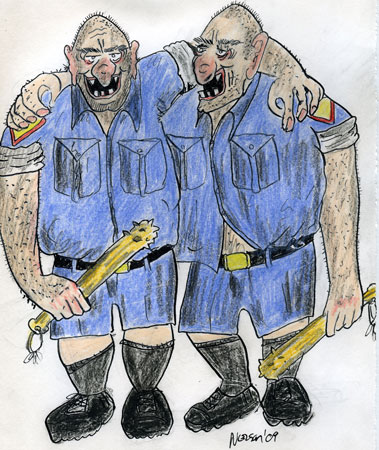
\includegraphics[height=60mm]{corps/chapitre19/img/personnage-papyblues.jpg}
\end{floatingfigure}

Le lendemain, alors que Timothée, toujours privé de son dispositif personnel polyvalent et de sa Saguewanish, était descendu au sous-sol du Centre faire libérer le père Jean, il s’était également occupé des deux frères Papyblues. Que leur reprochait-on, au juste, à ces malabars ? D’être grands, musclés, laids, bêtes, dangereux, terrifiants, d’avoir les dents sales, les ongles noirs, la mâchoire à figer le sang et d’appliquer, sans questionnement, les directives qu’on leur signifiait ? Avaient-ils déjà tabassé des bénéficiaires ? Non ! Avaient-ils déjà torturé des prisonniers ? Pas plus ! Avaient-ils déjà cloué des chats, provisoirement vivants, sur les portes de leurs geôles ? Que nenni ! Avaient-ils déjà coupé des rats en fines lamelles pour faire cuire un chow mein ? Encore moins ! Avaient-ils déjà dévoré de petits enfants, en commençant par la tête ? Absolument pas ! Le CS-1 leur avait fait alors une proposition de recyclage. De deux choses l’une, soit que les méchants gagnent, soit qu’ils perdent, et, advenant le deuxième cas, il y aura un important ménage. Un ménage de fond en comble.

- Si vous marchez avec nous, vous gardez votre job. En cas contraire, vous vous retrouvez, d’ici un mois maximum, sur la terre paternelle, dans l’arrière-pays. Donc, vous faites quoi ?

L’un des frères Côté avait grimacé un rictus à faire frémir le plus redoutable des gladiateurs du cirque Maxime sous l’empereur Trajan.

- On n’est pas con, chef ! On t’a vu aller. On sait qu’il y a ceuze pour qui les patates sont collées au fond, p’is qu’y a ceuze pour qui le party est à veille de pogner. Nous autres, on aime ça les partys !

Timothée avait alors souri et avait tendu la main. En l’écrasant, sans aucune malice, les deux Papyblues étaient devenus les gardes du corps de Marie et Romain. En poste 24 heures sur 24 chez Timothée, ils faisaient en sorte que le pire des scénarios, celui selon lequel Pete Barrett s’en prendrait aux personnes du couple Rioux-Tardif pour tenter de désarmer le groupe, s’avérerait désormais impossible. Sauf, qu’ils bâfraient comme des déchaînés et Timothée devait mettre ses amis à contribution pour renflouer ses armoires. Consulté sur cette importante question de sécurité, le colonel Alcide et son adjointe l’adjudant-chef Tremblay, une adjointe de plus en plus … intime, avaient averti tous les autres membres du comité «Mord-bec» d’être extrêmement prudent et, quand ils se retrouvaient seuls, de toujours avoir leur DPP en mode captation vidéo. Heureusement, un événement lourd de conséquences était venu régler le problème logistique causé par la goinfrerie des Papyblues.

En annonçant le projet pilote et les mesures soi-disant temporaires qui l’accompagnaient, le ministre Turcotte était devenu, pour les uns, une sorte de héros, un homme de compassion, de cœur, de sentiment, un personnage public honnête qui reconnaissait avoir peut-être commis des erreurs avec sa loi 173, un humaniste pour qui le bien-être et la dignité des aînés primaient sur la performance budgétaire de l’État et sur sa carrière politique. Pour les autres, il était ce qu’il avait toujours été, un politicien tirant la poche de son bord, c’est-à-dire du côté de son électorat rimouskois, des régionaux très éloignés de Montréal qui, les veinards, bénéficiaient d’un régime humanitaire exceptionnel. Quoi qu’il en soit, en une semaine, si on en croit les sondages et les vox-pop, il avait dépassé Ti-Dédé dans l’estime populaire et était de loin, la personnalité québécoise la plus admirée. Les éditoriaux l’adulaient, les talk-shows se l’arrachaient, les corps intermédiaires s’organisaient pour que dans leurs régions, la même chose se produise, il était invité partout où il y avait une plateforme. Même sur l’île d’Anticosti, la colonie de vieux squatters commençait à donner signe de vie et à communiquer avec l’entourage de l’homme politique. Avec l’âge, certains résidents semblaient préférer être rapatriés sur le «continent».

Sa gloire était telle qu’il s’était pris à son propre jeu et, en un mois, était devenu franchement convaincu qu’il fallait aller dans le sens des revendications du comité «Mord-bec», ce qui avait frustré bon nombre de profiteurs du régime. En fait, Turcotte s’était retrouvé tellement imbu de sa nouvelle importance et de son enviable réputation, qu’il avait juré aux parents de Timothée, un jour où la Maririou l’avait à nouveau convoqué sur la rue Crouet et qu’il s’était inquiété de la présence des sinistres frères Côté, que jamais au grand jamais, il n’accepterait, ni ne couvrirait, ni ne tolérerait toute exaction, violence ou autre vexation commise à leur endroit ou à celui de leurs amis, cela articulé solennellement devant trois caméras et quatre témoins. Il avait été tellement convaincant que peu après, les Papyblues avaient été retournés au Centre pour aider aux innombrables transformations en cours.

Au fil des mois, le projet avait pris corps. Confirmé dans sa tâche de directeur des loisirs, Robespierre avait tout de go commencé à en mener large avec l’aménagement du gymnase et de la piscine, dont il avait confié la responsabilité à son adjoint de fraîche date, Shimoune Saint-Pierre. «Tu viens faire splish splash avec moi, mon beau Robie ?» L’héritier du Pétépano avait également dû se dépêcher de nommer Bea Bellow responsable de la transformation de la salle du CA en bibliothèque. La vieille dame ne se souvenait pas d’avoir été aussi heureuse dans sa vie. Quant à Louise Lavoie, elle pouvait à peine l’aider, aux prises elle-même avec une collection quotidienne d’ennuis matériels défiant l’imagination la plus débridée.

La veille du début des travaux visant à en refaire un gymnase, le salon du personnel avait servi à recevoir la quasi-totalité des employés où l’ancien commando du 29 juillet 2033 qui s’était octroyé la totalité des sièges au comité de coordination avait répondu à toutes les questions et expliqué toutes les conséquences du changement d’orientation de l’établissement sur les postes. Si plusieurs demeuraient inchangés, de nombreux disparaissaient et d’autres étaient à combler, par exemple en alimentation, en entretien ménager, en loisirs, en soins infirmiers, en assistance gériatrique, en encadrement de bénévoles et ainsi de suite. Les intéressés n’avaient qu’à se manifester. Tous ceux qui voulaient conserver leur lien d’emploi étaient les bienvenus. Mais ils devaient méditer sur le fait que toute forme de malhonnêteté, d’abus, d’extorsion, de manquement éthique, de violence, physique ou verbale, et autres turpitudes à l’endroit des bénéficiaires, ou des locataires comme on les appellerait sous peu, serait immédiatement sanctionné par un congédiement sans appel avec rapport détaillé sur le certificat de licenciement.

Dans les deux mois qui avaient suivi, plus de 35 % des effectifs avaient choisi de partir, dont plus de 70 % des chefs de section et des cadres. «Bon débarras !» s’était écrié le colosse en apprenant la démission du gros Lavoie et du redoutable Pierre Monger, ex CS-1 du 4e Sud. En revanche, le départ de Claude Sey voulant retourner à l’université compléter un doctorat en ethnologie, l’avait profondément chagriné, tant il appréciait l’honnêteté et l’idéalisme altruiste du jeune homme.

Côté informatique, Vlado Marcovsky avait décidé de rester en poste et, à la demande du Comité, avait fait table rase de l’erratique système panrégional pour en implanter un nouveau entièrement basé sur du logiciel libre. Une enquête avait démontré que le diagnostic posé peu avant sa mort par Pierre Asselin, un vieil ingénieur quasi aveugle placé sous la responsabilité de Timothée, avait été juste. Il y avait effectivement eu tatouage de puces. Marcovsky et son équipe avaient eu besoin de quatre mois, incluant le temps de débogage, pour tout refaire. Il est vrai qu’il n’y avait plus de bénéficiaires à gérer, par contre les projets de recherche, en raison de l’implication de l’université et des travaux du docteur Bellavance, abondaient.

Pendant ces mois fébriles, rien n’était plus drôle que de voir Robespierre entrer, sans jamais frapper, dans le coqueron mal aménagé – merci Louise Lavoie - qui servait d’officine au gérant Carl Michaud pour lui faire signer des documents qu’il lui interdisait de lire. Amaigri, accablé, la peau grisâtre, l’ancien DG semblait au bord de la dépression. Dans les premiers temps de son calvaire, il avait essayé de plaider la cause de Philippe Dauphin. Mais le comité de coordination avait rejeté la demande. Flipper avait été bouté hors de la région avec promesse que si jamais on entendait à nouveau parler de lui, on le traquerait et on l’offrirait en pâture aux Papyblues. Il avait ensuite tenté sa chance avec Amédée Chicot sans plus de succès. On lui avait alors garanti qu’advenant que l’on retrouve cet abominable personnage, on en ferait une attraction populaire en l’enchaînant à vie, dans une cage bien en évidence au rez-de-chaussée du nouveau Centre, avec, pour nourriture exclusive, du Nutrisuz à saveur de poutine aux similis bacon.

Lentement, tout au long d’août et septembre 2033, la plupart des pensionnaires avaient été déménagés soit dans les familles, soit dans des hôpitaux, en attendant que les travaux soient complétés. Robespierre n’avait plus été sollicité pour des pilules du bonheur. Ceux qui avaient choisi de rester au Centre avaient été relogés temporairement au dernier étage, territoire naguère terrifiant qui venait de se transformer en colonie de vacances pour vieillards n’ayant nulle part ailleurs où aller, dont l’éprouvant Jean Saint-Gelais, le tandem aux mœurs discutables Thériault – Labbé et Luce Morency.

- Madame Thériault, vous seriez gentille d’avoir un œil bienfaisant sur madame Morency, avait demandé Timothée, désormais responsable de la dizaine d’employés affectés à cet étage. Il lui arrive de fuguer…

- J’me souviens d’elle au lac Saint-Mathieu. Belle femme, la Luce Morency …

- Moi aussi je me souviens, madame Thériault, moi aussi.

- J’vas m’en occuper, chef, fais-toi-z-en pas. J’y ferai pas mal !

- Profitez-en, vous et madame Labbé, pour vous installer dans la «p’tite chambre» de l’ancienne aile sud, à l’autre bout. Y a personne dedans. Vous allez avoir euh … la paix. En tout cas pour un bout de temps.

- Ça te dérange p’us qu’on soit gouines ?

- Ça ne m’a jamais dérangé, madame Thériault.

L’ex CS-1 avait à peine eu le loisir de s’approcher des ascenseurs que la vieille Loubert l’avait interpellé.

- B’en beau vos réformes, chef, mais moi je n’ai plus de sacs depuis une semaine. Vos gars, ici sur l’étage, ils savent pas où en trouver.

- Je m’en occupe, madame Loubert.

Une heure plus tard, Timothée réapparaissait avec une lourde caisse contenant de quoi satisfaire la victime de colostomie pour au moins un an.

C’était il y a dix mois, alors que tout était à faire. Aujourd’hui, dans cette salle d’audience trop climatisée, compte tenu des froides averses qui s’abat sur l’Est-du-Québec depuis près d’une semaine, Timothée qui n’entend plus rien, regarde tous ces gens qui, autour de lui, s’affichent ouvertement fous de joie, la plupart ayant attendu à la dernière minute pour lever un petit doigt d’appui. Heureusement, certains ont mérité d’être de la fête. Ici, Shimoune avec son ami de cœur, un ergothérapeute récemment embauché, là, Robespierre tenant Marie-Odile par la taille. Plus loin, Claude Say en séance de congratulation en compagnie du vieux Romain, encore plus loin, Béa Bellow et Louise Lavoie en train de rire aux éclats avec les frères Côté, près d’elles, Mmes Thériault et Labbé encadrant Luce Morency qu’elles ont vêtue d’un tailleur marine et dont elles ont coiffé les longs cheveux en chignon 1900, puis, à quelques mètres à sa gauche, Béatrice, SA fille sous la lanterne, occupée à converser en toute gentillesse avec un couple de médecins fraîchement recrutés et diplômés de l’Université de Montréal, deux jeunes idéalistes venus prêter main-forte à la contre-réforme du gros Turcotte. «Allez Béatrice, rends-les accrocs de ton charme !» Embauchée par l’UQAR, elle assumait depuis quelques mois la coordination des activités en recherche-action gérontologique et gériatrique que déployait le centre de haut savoir.

\begin{floatingfigure}[l]{40mm}
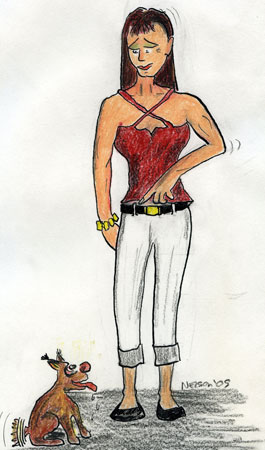
\includegraphics[height=60mm]{corps/chapitre19/img/personnage-beatrice-gazou.jpg}
\end{floatingfigure}

Quand leurs yeux se croisent enfin, le sourire de l’infirmière change aussitôt de registre. De socio-amical qu’il était, il devient beau, irrésistible, brûlant, amoureux. Partout, dans chaque capillaire de Timothée, dans chaque cellule de sa peau, dans chaque atome de tissu, une sensation enveloppante de bonheur, de chaleur, d’attraction, d’émotion, vient investir toute la place organique. Ce qu’il contemple alors, ce qu’elle le voit contempler avec une telle ardeur, ce n’est pas seulement une de ces femmes de rêve, «solitaire dans la foule comme en forêt», une de ces «femmes d’espoir heureux» telles que chantées naguère, des femmes que l’on mérite «en restant libre». Non. Ce qu’il voit, c’est cette femme qu’il vénère à chaque instant, cette femme qui, depuis près d’un an, le rend heureux le matin, le midi, le soir, la nuit, cette femme qui lui a fait oublier, revoir, réorganiser, repenser, 44 ans de vie pas toujours facile, une vie de gras du bide chauvasson et barniqueux. Il doit s’approcher, étirer l’instant de vertige, il lui faut aller goûter cette source d’apaisement, il doit aller entremêler son aura dans celle, toute en douceur enveloppante, de Béatrice. Plus rien ne peut le retenir.

- Timothée, viens, faut que j’te parle.

C’est la Maririou.

- Viens voir, j’ai quelque chose à te donner.

Un peu pour faire contre mauvaise fortune bon cœur, Timothée s’extirpe lentement de son envoûtement et suit sa mère qui navigue dans la foule comme une mamie impavide brandissant un terrible parapluie. La porte franchie, elle entre dans un grand vestiaire et, sur une tablette en haut des cintres, prend un sac de jute, une de ces poches dans lesquelles, à Saint-Anaclet, elle conservait d’innommables produits de son jardin.

- Là, ton père p’is moi, ils viennent de nous ressusciter légalement. Ça veut dire deux choses pour moi. Un, je deviens directrice de l’École de musique et on commence demain matin. Deux, je débute comme directrice musicale d’un orchestre de chambre et on donne un premier concert dans six semaines. Ça fait trois mois que je recrute des musiciens en cachette. On est rendus à 27, de tous les âges, et la plupart ont un passé professionnel. Ton père va même y être clarinettiste.

Timothée a pâli.

- Mais moi, je vais me contenter de diriger, je ne suis plus une bonne violoncelliste. Mes vieux doigts ne suivent plus. P’is toi, mon tit garçon, rassure-toi, je ne veux pas que tu en fasses partie avec ton cuivre à coulisse. N’aie pas peur ! T’as jamais aimé cet instrument et tu en as toujours joué parce que c’est moi qui l’exigeais, pour me faire plaisir, pour m’obéir, pour que je te foute la paix …

- Euh …

- … ou, peut-être, pour que je m’intéresse à toi.

Son regard fixant les portes de la salle, elle lui tend le sac.

- Tiens, c’est pour toi.

Timothée s’en empare et y enfouit son avant-bras où il découvre un étui en tissu capitonné un peu plus étroit, mais à peine, que celui de son trombone.

- C’est quoi ?

- Ouvre, tu vas voir ! Ça vient du Pays de Galles, c’est fabriqué par un artisan et on me l’a livré hier. C’est quelque chose qui va peut-être t’aider à te trouver, toi, un être libre que sa vieille folle de mère a trop longtemps essayé de modeler à sa façon, ce qui t’a empêché, pauv’ tit garçon, d’être dans la vie ce que tu étais dans ton petit cœur. J’ai tout compris ça en me débarrassant de la haine, de la peur, de la rage que j’éprouvais constamment à cause de mon père. La paix m’est venue, comme ça, après avoir réglé son cas au gros Turcotte, en lui arrachant les dents. J’ai pu tuer ma rancœur, étouffer ma maladie, pisser tout mon vinaigre.

Incrédule, inquiet, impressionné, curieux, le fils ouvre l’étui et y découvre une lyre.

- Une lyre ?

- Une lyre Sutton Hoo, mais à sept cordes, le même symbole de lumière et d’harmonie que la lyre dont jouait Timothée de Milet, le Grec qui a changé la musique pour éviter qu’elle ne le change, lui. Un homme qui avait compris que la vie, il fallait la vivre à sa façon et non à celle des autres, incluant, probablement, sa mère.

Les mots ne viennent plus à Timothée, embouteillés, qu’ils sont, dans un goulot bien étanche.

- C’est ton instrument, maintenant.

Et elle le gratifie d’un des rares sourires en 83 ans de parcours, un sourire si beau qu’il en ressent un grand bien-être. Puis, elle lui tapote doucement l’épaule et s’en retourne, de son trot de petite vieille pressée, vers l’intérieur de la salle d’audience.

- Apprends à en jouer, lui crie-t-elle avant de disparaître.

Penaud, les yeux rivés sur la lyre, il est figé, incapable d’exprimer quoi que ce soit. Béatrice qui avait observé la scène s’approche pour le tirer de sa catatonie.

- Viens, Timothée, on s’en va chez nous.

Dans le taxi de Jawad Kebbaj, avec son bouleversant cadeau sur les cuisses et un feuillet d’instructions en main, il dira :

- C’est diatonique, do, ré, mi, fa, sol, avec les deux cordes d’extrémité en la.

Puis, devant la maison de la rue Crouet transformée, depuis l’arrivée de la belle infirmière, en cottage coquet décoré d’arbustes, de fleurs et de rideaux, gratifié d’une peinture récente ainsi que de volets neufs et complété d’une clôture aussi inutile que mignonne, il ajoutera :

- Ce qu’elle vient de me donner, maman, ce n’est pas une lyre, mais la liberté. Ma liberté.

Sympathique dans sa gentille malice, Jawad fixera alors les yeux de Timothée dans le rétroviseur :

- J’ai l’impression, mon jeune homme, que tu fais mentir un vieux proverbe marocain qui dit : «Ouvre tes yeux avant le mariage, car après, tu ne pourras que les fermer». Dans ton cas, même si tu la maries pas, ta moukère, je la regarde et je sais que tu n’auras jamais besoin de les fermer tes yeux. Et ça, crac ! Ça défie la sagesse ancestrale du Maroc. Ou you-you ! C’est terrible ça, mon jeune homme, je t’le dis ! Tellement, ajoute-t-il en annulant son taximètre, que j’ai pas d’autres choix, tabarnak, que de te faire cadeau de ce voyage.

À l’intérieur, Timothée descendra un instant au sous-sol, dans le petit logement qu’occuperont encore quelques semaines ses parents avant de devenir locataires au Centre Sylvain Turcotte, pour utiliser la nouvelle désignation de l’ancien CRG, et, suivi d’un chien-rat en furie qui, apercevant la belle Béatrice, se paralysera à ses pieds, réapparaîtra avec son trombone. En prenant son temps, il le regardera, puis le replacera délicatement dans son étui. Il ajustera les trois fermetures et ira ranger ce témoin des 35 dernières années sur la plus haute tablette de son garde-robe.

Alors, avec respect, il soulèvera sa lyre galloise et commencera à en pincer les cordes.

- De toute ma vie, je n’ai jamais entendu un son aussi beau.

Un son n’ayant d’égal que le sourire qu’affichera alors Béatrice.

FIN

%\Titre{Postface}

\begin{Postface}

On peut dire, puisque de nos jours il faut toujours savoir tout caser et être en mesure de le faire avec brio, que «Le joueur de lyre» est un roman-blogue, un exercice Web 2.0, où un blogueur a bricolé une histoire en se connectant sur l’imaginaire, la connaissance, la culture, la générosité, le sens critique et le potentiel ludique de ses visiteurs-lecteurs-commentateurs. Voilà de quoi attirer l’attention des experts ès blogosphère et recevoir la médaille du mérite cybernétique. Mais dans le fond, «Le joueur de lyre» n’est qu’une simple aventure «littéraire» – souffrez que j’utilise ce terme - qui par-delà la mécanique Web, celle du portail Cyberpresse, de la masse d’abonnés, du logiciel WordPress et de l’infrastructure de télécommunications, puise dans une source éprouvée, celle du conte comme il s’en dit depuis la nuit des temps, depuis qu’il y a des enfants à aimer, à bercer, à faire glisser, tout doucement dans la dimension du rêve. Rappelez-vous, si vous avez eu ce bonheur, comment on raconte une histoire à un jeune enfant, le soir après le bain, après le petit pyjama, juste avant le dodo.

- Conte l’histoire du petit renard.

- Hum, celle où la poulette le chasse avec ses petites ailes en bataille ?

- Oui.

- OK. Hum ! Il était une fois, un vieux poulailler mal peinturé au milieu d’un enclos clôturé avec de la broche, où vivait une belle petite poule rousse…

- Non, pas rousse la poule, blanche.

- … où vivait une poulette toute blanche avec huit petits poussins tout jaunes…

- Non, elle n’avait pas de poussins, c’est sa maman qui en avait.

- OK c’est sa maman. Un jour, alors qu’elle grattait le sol avec sa petite patte à la recherche de nourriture en compagnie des petits poussins, elle vit se faufiler près du grillage, un petit renard …

- Tout maigre le petit renard … ehhhh, il faut dire renardeau …

- … un renardeau tout maigre qui n’avait rien mangé depuis trois jours.

- Il n’avait pas de maman, le renardeau ?

- Euh, elle était malade sa maman.

- Elle avait quoi ?

- Elle s’était fait mordre par un gros méchant chien très laid …

- Laid comment ?

- Pire que le chien de madame Rioux.

- Ouache… Je l’aime pas ton histoire.

- Elle ne pouvait pas aller chasser, la maman, et c’est le petit renard qui devait lui trouver de quoi se nourrir.

- Pauvre petit renard !

- Ouin ! Un jour, donc, la petite poule blanche aperçoit le petit renard et, les ailes abaissées, se met à caqueter très fort, comme pour dire : «Alerte, un renard, alerte !»

- Par où il pouvait passer, le petit renard, s’il y avait de la broche ?

- Les ratons laveurs avaient fait un trou dans le grillage et le fermier l’avait mal réparé.

- C’est méchant des ratons laveurs ?

- Non, pas vraiment.

- Ahhh.

- Donc, quand il a constaté qu’il avait été découvert, le petit renard s’est mis à pleurer. La petite poule blanche s’est approchée et lui a dit …»

Et ainsi de suite. C’est toujours ainsi. Vous avez une histoire dans la tête, c’est-à-dire un début, une fin et, entre les deux, un écheveau de faits et un début de collection de personnages. Au fur et à mesure que vous la dites, le bout de chou vous force à ajouter des détails, des séquences, des nuances, vous amène à revoir le ton, le débit, voire la morale et, surtout, vous permet de juger si vous êtes intéressant, ennuyeux ou assommant. C’est génial ! Il en est ainsi pour le roman-blogue. C’est un conte sain, simple et enrichissant, un exercice littéraire amusant, un jeu d’enfant, un jeu d’éternels enfants en quête d’émerveillement que nous serons tous jusqu’à la fin. C’est à l’opposé de ce qu’un auteur va fabriquer dans le silence, l’inquiétude et le doute, sans ces nutriments essentiels pour les uns, superflus ou redondants pour les autres, que sont l’interaction et la critique en direct.

Une autre considération à relever est la dimension feuilleton dans laquelle s’est drapé «Le Joueur de lyre». Inspiré à tort ou à raison par les grands écrivains du XIXe siècle, j’ai fait le pari de mettre un chapitre en ligne tous les vendredis matin et … je l’ai perdu. Effectivement, il m’a été impossible de le faire le 2 janvier 2009 en raison d’obligations familiales particulières au Nouvel An et de l’incontournable réalité d’un voyage à l’étranger. Reste qu’on parle de 20 semaines, de 19 chapitres, d’une quarantaine de dessins et de près de 132 000 mots (si je ne tiens pas compte de cette postface), soit une moyenne de 6 600 mots et deux dessins par semaine. Or il s’adonne que, durant cette période, mes vies personnelle et professionnelle ont exigé de très nombreux déplacements au Québec, en Ontario et, surtout, aux États-Unis. Tant et si bien que des chapitres entiers ont été écrits en auto, en avion, dans une chambre d’hôtel, dans une salle de presse, dans un sous-sol de Rimouski et même dans une tente de prospecteur, je vous jure ! J’entends d’ici la critique affirmer qu’à un tel rythme et dans de telles conditions, aucun roman digne de ce nom, ne pourra naître. À plus forte raison que l’auteur n’est pas un romancier, mais un journaliste. Un pisse-copie qui dessine de petits mickeys pour illustrer sa prose. Ça ne fait pas sérieux !

C’est là où, encore une fois, la techno vient déjouer ceux dont la pensée acquise est prodigieusement structurée, articulée, documentée, mais pleine d’inconnus par rapport au potentiel créateur des nouveaux outils.

Revoyons le processus que j’ai appliqué dans le cas de cette histoire de vieux Baby Boomers à qui les générations X, Y et Z font payer leurs vies dissolues.

Étape un : Récapitulation de la trame, articulation de la séquence du chapitre en cours, précisions des faits afin qu’ils soient plausibles, réflexions sur l’aspect humain des personnages mis en scènes dans ce chapitre. Cette étape a systématiquement été accomplie en discutant seul à seul avec ma conjointe, très souvent en auto.

Étape deux : Recherche dans les livres et sur le Web pour des explications généralement scientifiques et, parfois, pour des bouts de chanson dont j’ai oublié des paroles. Il y aura aussi des coups de téléphone, des échanges de courriel, des rencontres formelles afin que l’on m’explique ou me décortique un détail important.

Étape trois : Premier jet d’écriture et première version retravaillée et nettoyée de la majeure partie de ses fautes (merci Antidote !). En moyenne, j’ai eu besoin d’une vingtaine d’heures pour cette étape.

Étape quatre : Dessin de deux personnages et mise en ligne du chapitre illustré. Ajoutez ici un bon deux heures.

Étape cinq : Rétroaction grâce au système de commentaires offert par le logiciel WordPress. Dans les cinq ou six jours suivant la mise en ligne du chapitre, les lecteurs ont pu qualifier leur appréciation, suggérer des améliorations, critiquer un choix d’auteur, souligner et corriger des fautes et débattre d’un point soulevé. Jour après jour, j’ai pris connaissance de ces commentaires et, la plupart du temps, j’ai rapidement apporté les changements souhaités et les corrections qui s’imposaient. Parfois, cela m’a obligé de retourner en arrière dans des chapitres déjà publiés.»Vous maîtrisez avec perfection l’art de se r’virer sur un dix cennes», a écrit bibelot (pseudonyme d’une commentatrice devenue essentielle au sujet de laquelle je reviendrai plus loin). Ainsi, chaque chapitre se retrouve bonifié, épouillé, resserré, bref, réécrit. Certains connaîtront plus de dix versions, d’autres trois ou quatre. stvcc s’est dit impressionné par cette façon de faire. «Faut être humble en titi». En moyenne, j’ai eu besoin d’une dizaine d’heures pour cette étape, une étape qui, la plupart du temps, est venue se chamailler avec l’Étape trois.

Étape six : Une fois les dix-neuf chapitres commentés et retravaillés, je les ai polis d’une réécriture finale. Dans certains cas, p. ex. les chapitres 17 et 19, ce fut majeur. Dans d’autres, p. ex. les chapitres 5 et 13, ce fut mineur. C’est également à cette étape que j’ai rédigé la préface dans sa forme actuelle.

Étape sept : Rédaction du bilan que vous êtes en train de lire.

Ce que je viens de vous soutenir, c’est qu’en une semaine, période où j’ai quand même à assumer ma charge professionnelle de journaliste techno pour deux médias, un chapitre a été écrit de la plus belle façon que je le pouvais et publié sur mon blogue dans Technaute.ca, tandis qu’un autre a été scruté, corrigé, nuancé, bref, amélioré. Tout cela, dois-je le préciser, sans jamais utiliser une imprimante.

Ne serait-ce que par le temps impliqué, on est loin du fonctionnement traditionnel où l’auteur expédie par la poste (dans le cas d’imprimés) ou par courriel (document électronique) un chapitre à des amis ayant été embrigadés dans un «comité de lecture». Dans mon cas, je n’ai pas eu besoin d’une telle structure «amicale», puisque 56 abonnés à la Cyberpresse se sont portés «volontaires». C’est qu’au cœur du concept Web 2.0, il y a la notion de «communauté», et «Le joueur de lyre» a rapidement eu droit à la sienne, une communauté polie, drôle, généreuse et cultivée juste assez grande pour que je ne perde pas le nord.

\begin{floatingfigure}[r]{40mm}
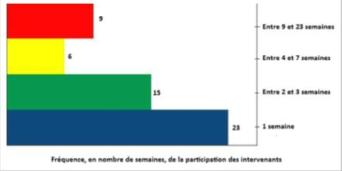
\includegraphics[height=60mm]{intro/postface/img/illustration2009021302.jpg}
\end{floatingfigure}

De ces 56 intervenants, 9 se sont manifestés sur au moins neuf semaines (dont 5 pendant plus de 15 semaines), 6 entre 4 et 7 semaines, 15, entre 2 et 3 semaines, 23 sur une seule semaine et un l’a fait au téléphone. Ici je ne calcule pas le nombre d’interventions où ces gens se sont exprimés dans la (ou les) semaine(s) où ils sont intervenus. Ce nombre a fluctué entre 10 (semaine du 26 décembre) et 102 (semaine du 19 septembre), sans qu’aucune tendance vers la baisse ou vers la hausse du nombre de commentaires ne se soit dégagée. On peut donc parler d’une communauté constituée d’une quinzaine de réguliers et d’une quarantaine de commentateurs plus discrets, des gens moins enclins à prodiguer leurs grains de sel.

Force m’est de signaler que sur les 56 participants, j’en connaissais sept :

    albel : mon beau-frère de Trois-Rivières. Fréquence : une semaine.
    alexanticosti : j’ai correspondu avec lui avant d’être à la Cyberpresse, mais je ne l’ai jamais rencontré. Fréquence : 15 semaines.
    jpmononk : un vieux copain depuis toujours. Fréquence : 3 semaines.
    laouise : une amie originaire de Rimouski. Fréquence : 13 semaines.
    madgab : ma grande fille bien-aimée qui est venue faire son tour sans m’avertir. Fréquence : une semaine.
    rejeanp : un vieux copain de longue date. Fréquence : aucune; il a utilisé le téléphone.
    snouppix : un vieux de la vieille que je connais depuis une quinzaine d’années. Fréquence : une semaine.

Ces gens, tous masqués d’un pseudonyme comme c’est la coutume sur Internet, des gens dont j’ignore l’identité (sauf ceux mentionnés ci-haut), bref de purs étrangers, m’ont fait le cadeau de nombreuses suggestions très utiles et sans lesquels la livraison du produit dans les délais prescrits n’aurait été possible.

Certains m’ont proposé des remaniements importants. Un bel exemple est cette suggestion qu’a publiée claude_c, le 5 septembre :

    «Bonjour Nelson, je vous propose, bien humblement, des coupures et aménagements, de façon à rendre le texte plus dynamique, et qu’on découvre les personnages plus rapidement. Certaines descriptions m’ont paru, à ce stade du récit, superflues. Mais il n’est pas dit que vous ne devriez pas les conserver pour la suite, au contraire. Vous en faites ce que vous voulez.»

Et là, le gars m’a copié-collé tout mon chapitre UN de la façon où lui l’avait redécoupé. Comme l’amélioration était majeure, je me suis empressé de l’accaparer et de faire les changements nécessaires.

D’autres ont pointé sur des passages qui mériteraient d’être un peu mieux tartinés. C’est le cas de cette suggestion de marcofsky qui est apparue le 2 novembre.

    «Le chapitre précédent annonçait un pivot dans l’histoire et on le sentait bien. Les événements de ce chapitre confirment cela, mais je trouve que l’intensité y fait un peu défaut. Par exemple, le dépucelage de Timothée: c’est un moment important, surtout que ça arrive à 43 ans ! N’y aurait-il pas lieu de “beurrer un peu plus épais” ? Mais surtout, de faire sentir au lecteur que, pour Timothée, cela a changé quelque chose. Idem pour la scène où on présente la lettre - je ne sens pas la “gravité” du moment, ni la surprise de Timothée ou celle de son père. Mais remarquez, c’est très subjectif ce que je dis, ce n’est qu’une impression.»

Et on m’a suggéré des réécritures. Par exemple ce paragraphe que m’a envoyé suzkinne, le 22 janvier, à la suite de commentaires sur ma nouvelle préface, paragraphe que je me suis dépêché d’aller coller en lieu et place du mien :

    «Il arrive quoi dans un sous-sol démoralisant, anémiant et sale, lorsque des gens jusque-là prostrés, cloîtrés et gommés des registres, se mettent à vivre toute une gamme de sentiments humains, partant de vieilles blessures cachées bien creux qui s’ouvrent, passant par des décennies de non-dit, de colère refoulée et d’ambitions détruites, finissant dans les larmes, le sourire et le bonheur ?»

Quelle chance j’ai eue, allez-vous dire. Attendez, il y a encore mieux. À plusieurs reprises, on m’a gratifié d’ajouts très intéressants dont certains ont contribué grandement à améliorer la qualité de mon histoire. C’est le cas de madgab qui, dès le chapitre 1, a surgi en ligne avec l’idée de créer un personnage canin, une sorte de chien hargneux et laid qui ajouterait à l’ordinaire des deux vieux illégaux enfermés dans leur sous-sol. Bibelot y est allé d’un prénom, Gazou, et d’un exemple de dialogue entre la vieillarde et son animal. Enfin, bernardprince a proposé un collier GPS qui permettrait au cabot de pouvoir faire sa promenade quotidienne sans avoir besoin d’humain ou de laisse. Quand on sait le rôle qu’a eu Gazou dans cette histoire, on ne peut que s’en féliciter.

C’est aussi le cas de dennis_dubeau qui a pensé à une pilule pour en finir, question de ne pas connaître le sort qui incombe aux vieux tel que décrit au chapitre 2. Encore une fois, Bibelot a fait du pouce et a suggéré un nom pour cet expédient, la «pilule du bonheur». C’est ce qui m’a amener à retravailler un rôle secondaire pour en faire quelque chose de beaucoup plus important, celui de l’ineffable Robespierre Alcide. Plus tard, le même dennis_dubeau a lancé l’idée de recourir au sabotage de la Saguewanish du chef de section Timothée Tardif. D’où le personnage du bonhomme Jean.

Et que dire d’albella qui, inopinément, m’a proposé une abomination sordide, soit un procédé de culture hormonale à partir de semi-cadavres. Cela a donné lieu à la naissance du sinistre docteur Bellavance, lequel, comme vous le savez maintenant, a fini par devenir gentil et attachant et s’est avéré très utile pour bien ficeler l’intrigue et le dénouement.

Autre bonne idée, alain_from_west a découvert une façon d’expliquer les pannes incessantes du système informatique utilisé au CRG-BSL. Selon lui, on aurait pu avoir recours à des «puces tatouées» rendant problématique l’utilisation de logiciels libres. Grâce à cette idée, il m’a fallu développer un personnage appelé Pierre Asselin, un vieil ingénieur logiciel quasi aveugle gardé dans une salle pour personnes en perte d’autonomie.

Pour sa part, suzkinne a fait deux interventions remarquées. Elle a commencé par nous produire une recette sérieuse du manger mou servi aux bénéficiaires, d’où l’appellation subséquente de Nutrisuz. Ensuite, elle nous a expliqué médicalement comment et pourquoi Marie Rioux était tombée malade, ce qui avait obligé Timothée à quérir l’aide du docteur Gagnon.

Parlant médecine, rejeanp, détenteur de je ne sais trop combien de diplômes universitaires en science, m’a corrigé le scénario médical de la mort du vieil anarchiste Robert Gagnon, alias Dart Vader. Commentateur occasionnel sur Technaute, il a préféré me téléphoner ses explications avant que je ne publie le chapitre en question.

Enfin, l’inénarrable flipper_21, grand praticien du calembour extrême, a suggéré d’utiliser le pseudonyme des contributeurs-commentateurs pour offrir des patronymes aux personnages secondaires de l’histoire. Sous un concert d’approbation, j’ai donné suite à cette idée dont voici le résultat.

    alain_from_west : Al Fromwest, partenaire informaticien de Pierre Asselin
    albella : le docteur Christian Bellavance, fermier hormonal qui n’avait jamais vu New York
    alexanticosti : Alessandro Costi, malfaiteur montréalais
    bernardprince : marque du collier GPS pour chiens solitaires
    bibelot : la bibliothécaire à sa retraite Bea Bellow
    bluesly et papynut : les frères Côtés, alias les horribles Papyblues
    claude_c : le jeune idéaliste Claude Sey
    dennis_dubeau : le chef des Verts, Thierry-Ian Dennis-Dubeau, alias Ti-Dédé
    flipper_21 : Phillipe Flipper Dauphin, le méchant directeur des communications
    jakeleblanc : le fonctionnaire économiste du Comité de déontologie Jacques Leblanc
    jpmononk : le représentant des bénéficiaires au Comité de déontologie, Jipé Gendron, alias Tit-mononk
    laouise : Louise Lavoie, responsable logistique au CRG-BSL
    marcofsky : Vlado Marcovsky, directeur de l’informatique au CRG-BSL
    rejeanp : le docteur Prévost, médecin légiste
    stvcc : joueur de cartes bègue appelé Steve Cécé en raison de son handicap
    suzkinne : Anton Suzkinne, inventeur du manger mou distribué par Monsanto sous le nom de Nutrisuz
    toogreen : l’agent de sécurité tropecolo
    ttc1 : L’agent de procuration Thomas Tremblay-Seyun, dans l’histoire des sacs de colostomie

D’ailleurs, voici la réaction de ce dernier commentateur en découvrant qu’il a inspiré un personnage. Très amusant !

    «Han ? Quoi ? Comment ? Moi ? “ttc1, l’agent de procuration Thomas Tremblay-Seyun (…)” ? C’est moi ça ? Woahhhh ! J’en suis toute chose. Non mais, m’as-tu me les taper les bretelles devant la galerie ! J’ai inspiré un personnage du premier roman-blogue de l’histoire québécoise (…). Je fais parti de la révolution Web 2.0 ! Whouhou ! C’est Warhol qui a dit que tout le monde avait son 15 minutes de gloire ? Je viens de vivre le mien. Merci Nelson !».

Mais toutes les suggestions n’ont pas été acceptées. La plus évidente est celle de prorats qui, comme l’indique son pseudonyme, voulait que j’ajoute des rats dans la description du CRG-BSL. Ouache ! Autre exemple, bluesly aurait aimé que mes personnages soient nantis d’implants électroniques sous-cutanés. Cette techno ne m’apparaissant pas comme pouvant être dominante dans 25 ans d’ici au point d’en faire bénéficier les vieillards, je ne l’ai pas retenue. Mais peut-être ai-je eu tort.

Et ce n’est pas tout. Qu’y a-t-il de plus désagréable à la lecture d’un roman, que de découvrir une erreur de fait. Par exemple, écrire que la violoncelliste Marie Rioux a joué pour l’Orchestre métropolitain de Montréal dans les années 70 alors que l’ensemble a été fondé au début des années 80. Ou aller visiter une dame dans son condo quand, deux chapitres plus tôt, on l’a fait vivre chez ses parents. Ou cacher un détail important à quelqu’un oubliant qu’on le lui a révélé trois chapitres en arrière. Ou être complètement à côté de la coche avec des horaires et des durées de trajet en autocar. Ou avoir camouflé des pilules du bonheur dans une boulette de papier aluminium alors qu’il y a des détecteurs aux portes du Centre gérontologique. Et ainsi de suite. À elle seule, la redoutable bibelot a débusqué huit de ces erreurs et suzkinne, deux. De quoi frémir !

Quelques-uns ont même accompli des tâches parfois fastidieuses, sans jamais demander quoi que ce soit. Comme ça ! Bénévolement ! Pour le plaisir ! La plus évidente et adulée de ces tâches est évidemment celle de bibelot qui, chapitre après chapitre, a tout récuré, sondé, soupesé, questionné et, d’un crayon rouge sang, corrigé. D’une semaine à l’autre, elle a imposé son autorité et a fait pâlir d’envie les linguistes et informaticiens à l’origine de la version d’Antidote que j’utilise religieusement. Étant personnellement victime d’une éducation bilingue, j’ai dû, en fin d’adolescence, réapprendre à écrire le français et … il est resté des traces. En plus, j’ai les doigts pleins de pouces et je tape à la diable. Bref, comme bien du monde, je fais des fautes. Parfois des gênantes. Des misères que je ne vois pas. J’ai beau comprendre «que je ne vois pas», en réalité c’est «que le de vois pas» qui est couché sur la page et je ne remarque rien. D’où Antidote ! Malgré cela, bibelot découvre de nouvelles «cidores». Voici ce qu’elle en dit:

    «Pourquoi je prends la peine de lire avec attention ? Par pur plaisir ! Depuis ma tendre enfance, je dévore tout ce qui se lit, même la boîte de céréales du déjeuner, sans blague. Votre roman-blogue me captive au plus haut point. Et traquer des cidores tient mon esprit en alerte.»

Et quand ce n’est elle, c’est Alexanticosti, suzkinne, flipper_21 et d’autres, dont laouise. «Cidores» ? C’est un acronyme de mon cru signifiant «coquille involontaire dont on regrette l’existence» (ce que marcofsky appelle «tapsus») qui, allez savoir pourquoi, s’est imposé dans les commentaires. De là sont venus les néologismes «cidoricide», «décidoriser» et «cidorigène».

Toujours à l’enseigne de l’aide désintéressée, il y a dennis_dubeau qui a écrit et enregistré un Blues inspiré par l’histoire de Marie Rioux qu’il a intitulé le «Blues de Gazou». Il y a également marcofsky qui, dès le départ, a offert ses services graphiques et qui a produit une galerie Web des personnages que j’ai dessinés. Quant à toogreen, l’homme de Shanghai, il a entretenu en ligne sur son propre blogue, une version PDF de mes chapitres.

Mais en plus de m’avoir fourni l’assistance nécessaire en raison du train d’enfer imposé par le mode feuilleton, ces gens anonymes m’ont fortement encouragé, pour parler en euphémisme. Ils m’ont permis de sentir, eux cette infime minorité d’internautes qui commentent en ligne, qu’il y avait du monde ici et là pouvant aimer ce que je faisais. C’est ce qui explique, chaque semaine, quand le doute venait frapper à ma porte, que je me raccrochais à eux et je continuais. Voici quelques exemples :

    «Ces personnages que vous avez su rendre attachants sont désormais ancrés dans mon univers imaginaire.» (bibelot)

    «J’étais tellement absorbé par la lecture qu’il n’y avait plus d’écran, plus de souris, plus de Technaute, rien. Rien que Timothée et cie.» (bluesly)

    «Personne ne pense plus à modifier l’histoire; on la suit comme du bonbon.» (dennis_dubeau)

    «Que les membres de mon entourage se le tiennent pour dit : ils vont découvrir un nouvel auteur au cours des prochains mois !» (flipper_21)

    «Cette belle histoire qui se termine ce soir, malheureusement (…) m’a donnée le goût de me remettre à … Lyre.» (jakeleblanc)

    «C’est déjanté, délirant et, en même temps, il y a de l’espoir. Les dessins sont extra, rien ne manque !» (laouise)

    «Merci pour ce beau roman sur lequel je suis tombé par hasard et que je me suis empressé de partager avec des amis dès ma lecture du premier chapitre.» (lewebiste)

    «Bon, parlons Art ! Parce que là, on y est ! Et pourquoi ? Parce que le conteur est maintenant à l’aise avec son récit et ses personnages. À l’aise également avec le rythme imposé soit un chapitre par semaine (…). Comme le musicien, c’est maintenant la mélodie qui l’anime et il ne pense plus à ses doigts, même s’ils sont occupés à jouer un solo d’enfer sur la guitare ! Le côté technique étant maîtrisé - et oublié - le talent peut maintenant être transcendé, tout bonnement par le plaisir ! Parce que c’est ce qu’on sent le plus dans ce chapitre, l’auteur a eu du plaisir à l’écrire. Et ça nous procure un plaisir unique à nous qui le lisons: ce n’est plus une question de style ou de genre, ou encore de pirouettes ou de bons mots, ça devient homogène et on le reconnaît : C’est le plaisir de lire du Dumais ! Merci, Nelson !» (marcofsky)

    «Quant à l’émotion qui se dégage de ce chapitre, j’en suis encore un peu gaga après une seconde lecture.» (papynut)

    «J’ai vraiment aimé l’histoire. Même que, pour mon cours de français, j’ai fait un exposé oral sur votre roman.» (ph.mongeau)

    «Si j’avais le roman en main, je ne pourrais interrompre ma lecture, je crois que le lirais tout d’une traite.» (suzkinne)

    «J’ai toujours hâte de lire la suite chaque semaine. Merci de prendre le temps de l’imaginer et de l’écrire.» (technaute.spamfree)

    «D’un chapitre à l’autre on ne peut prévoir la suite, c’est rebondissement sur rebondissement. Ça pourrait devenir très mélangeant et décousu, mais non, malgré tous ces intrigues et revirements, cette toile d’araignée se tient solidement sur ses ancrages et on suit le fil d’un chapitre à l’autre. (…) Les personnages sont vivants, crédibles et attachants.» (ttc1)

Si les commentateurs ont fait preuve d’autant de gentillesse, ils ne se sont pas privés d’amener des critiques pour autant, ce qu’ils ont toujours fait avec bonhommie, tact et délicatesse. Voici quelques exemples:

    «Fascinant! La Sociologie-Fiction a maintenant un nouveau chantre attitré: Nelson! Mais je ne suis pas aussi pessimiste. J’ai de bonnes raisons de croire que Nelson pousse le bouchon un peu loin lorsqu’il invente des chambres à gaz pour “réduire les coûts”. La tendance actuelle (ex. AQDMD) est plutôt vers plus de contrôle du “bénéficiaire” sur la date de sa mort plutôt que moins. Aussi, Nelson élimine un peu vite une autre tendance lourde, celle-là: la continuation du travail après l’âge canonique de la retraite, au moins pour ceux qui en retirent une certaine satisfaction. L’impact financier sera considérable. La vraie mort sociale c’est quand les autres n’ont plus besoin de nous.» (mvirard commentant le chapitre 2)

    «Comme je l’avais souligné dans le premier chapitre, je trouve que les informations incluses dans les blocs de descriptions ne sont pas assez livrées dans l’action. Dramatiser l’information. Et à mon avis, les descriptions contiennent trop de matières qui, pour l’instant, ne sont pas essentielles à la compréhension et au déroulement du récit. Si l’auteur tient absolument à les garder, pour alléger la lecture, il devrait les disséminer au fil du texte, au détour d’une réplique ou d’un paragraphe, pas nous les livrer en bloc. Et ne conserver que ce qui est nécessaire. Mais bon, c’est juste mon opinion, et ça vaut ce que ça vaut. (claude_c, à la suite du chapitre 2)

    «Ma seule critique sur le chapitre 19 serait que j’ai lu les 25 articles de l’entente en diagonale comme si de lire le contrat me sortait de l’histoire. La réplique de Romain à Turcotte est vraiment savoureuse… à partir de là, j’ai raccroché d’un seul trait jusqu’à la fin.» (bluesly déplorant la première présentation des articles imposés au ministre Turcotte)

    «Si cette œuvre se veut un véritable roman (…), alors mon ami Nelson, faut pas avoir peur d’y mettre tes tripes et de bonifier le document avec toute la gamme des émotions prévisibles dans ce type de situation. Personnellement je reste sur ma faim, j’ai l’impression de regarder un film sans dialogue et sans musique, C’est plutôt fade.» (alain_from_west sur une certaine sobriété qui avait caractérisé la première écriture du chapitre 7)

    «Les acronymes me distraient, car il me force à arrêter et à réfléchir sur ce qu’ils veulent dire… Ça ralentit le mouvement de l’histoire (…). Je préférerais les dénominations au long ou un synonyme, mais au long… (dennis_dubeau réagissant aux nombreux acronymes bureaucratiques que, dans un premier temps, j’avais parsemés ici et là pour faire encore plus Orwell)

    «Ce cinglé de Dart Vader m’a retourné l’estomac au point d’en avoir des convulsions (…). L’antithèse parfaite du Festin de Babette.» (bibelot au sujet de l’orgie alimentaire du chapitre 14)

    «Moi c’est ce qui a atterri dans le pare-brise qui me lève le cœur. J’en ai déjà eu un de même il y a plusieurs années ! Ouache ! Faut plus que j’y pense !» (lui répond laouise, référant à un geste de provocation posé par Robespierre dans le même chapitre.)

    «Ah ben prorats, t’aurais dû te taire ! Une chance que j’ai lu le chapitre avant la correction» (gemnoc qui réagit à la correction apportée à une répartie de la Maririou où j’avais oublié de la faire chuinter. C’est prorats qui avait signalé ce détail : «J’ai-tu manqué un chapitre ? La Maririou ne chuinte plus. Bonne nouvelle, ça va être plus facile à lire !»)

    «Un roman-blogue, cette invention que je n’ai toujours pas saisie !» (claude-henri, à la suite du chapitre 12)

    «Sincèrement, je n’ai jamais eu d’intérêt pour la Maririou. Je trouve que cela ne cadre vraiment pas avec le mandat de votre blogue. (…) Nous venons lire vos articles pour vos connaissances techniques et votre expérience et non pas pour lire votre passe-temps. Je vote pour la terminaison de la Maririou !» (lelecteuraverti amorçant un débat le 2 janvier; «La Maririou» était le titre de travail du Joueur de lyre.)

    «Je ne peux pas dire que le roman-blogue la Maririou est la partie que j’apprécie le plus de l’œuvre (de M. Dumais). Je suis un grand lecteur, je lis une vingtaine de romans par année, un par deux semaines environ, des polars principalement. (Mais) La Maririou, j’ai lâché après le premier chapitre. J’aime (…) le travail de M. Dumais lorsqu’il nous cause informatique (…).» wiiphone, le 2 janvier)

    «Je suis du même avis que lelecteuraverti. Je n’ai aucune idée de ce que fait cette nouvelle sur ce blogue qui n’est pas à sa base littéraire. Je me suis donc rapidement désintéressé de La Maririou. (…) J’avais, depuis un certain temps, tout simplement pris l’habitude de ne plus lire la chronique du vendredi. Maintenant que le sujet est sur le tapis, je sors du garde-robe avec mon opinion sur le sujet.» (nimzo, le 2 janvier)

    «Faut pas mal le prendre (mais) l’histoire ne m’intéresse pas vraiment. (…) Ce n’est pas pour moi. (Par contre), ce qui est fascinant pour moi, c’est l’interaction qu’elle provoque. (…) J’attends la suite des commentaires avec impatience. On ne voit pas ça souvent un auteur qui permet à ses lecteurs de le critiquer et de faire des révisions en direct.» (ianlambert, à la suite du chapitre 4)

Cette dernière remarque attire l’attention à juste titre sur l’interaction suscitée par le projet. Très rapidement, dès le chapitre un, les échanges entre commentateurs fusent de toutes parts. Le ton est, la plupart du temps, humoristique et des gens m’avouent les lire puisqu’ils sont … divertissants. Un trio se dégage assez vite de la mêlée, celui de dauphin_21, dennis_dubeau et alexantisosti. Certaines répliques sont totalement hors sujet, je les laisse quand même en ligne en raison se leur ton, de leur humour. Après tout, un roman-blogue, ce n’est pas une corvée canoniquement sérieuse, mais un divertissement collectif. Voici quelques exemples parmi tant d’autres tout aussi rigolotes:

    «Les Dumais, ça doit être fait forts en torrieu ; se placer ainsi sous la loupe (qui est la femelle du loup, tout le monde sait ça) d’une gang de téteux du dico, de la phrase juste, des régionalistes bien faits et du calembour à répétition (comme dans carabine à répétition). Je ne serai plus parfaitement objectif à la fin de cet exercice, alors je me garde trois ou quatre chum(e)s qui ont fréquenté Kerouac, Cavanna, Brétécher et Dard (pas l’épée là, le papa de Béru) à qui je me retiens à quatre sabots de refiler l’adresse de ce salon littéraire. Juste pour voir comment ça sera perçu, ce roman à multiples mains et une paire de nageoires… Entéka, ça ne devrait pas coûter trop cher en correction. J’ai aussi en réserve 3 amies (rien que des filles, tiens !) maniaques de la virgule bien placée, du parfait du subjonctif (plus difficile que l’imparfait du…) et amateuses de mots croisés, de l’Italie et de Falardeau (nobody’s perfect). Attends qu’elles passent sur ton texte mon Nelson, une horde de Bibelot. Ichhh. Allez mon Nelson, une double clef. Démolis-en quelques-uns. Tant pis si c’est des cousins. Fais-leur sortir le raisin. Faut que ça saigne.». (alexanticosti, le 28 octobre)

Le 14 novembre, un peu fatigué, j’ajoute à un commentaire de dennis-dubeau que j’aimerais pouvoir me consacrer à ce projet à temps plein et que j’en ai un peu marre, à ce jour, d’en avoir livré la moitié sur la route, dans des conditions peu propices à l’écriture. Ce à quoi ledit dubeau me répond :

    «Et qu’est-ce qui vous oblige à courir ? (…) Vous pourriez vous alléger la vie et rendre ce processus encore plus agréable pour vous en sautant une semaine sur deux ou en variant, un texte par mois ou par trois semaines. Ça vous laisserait respirer et nous, on aurait encore plus de fun créé par l’attente ! (…) Il n’est écrit nulle part que ceci doit se terminer CHAQUE vendredi !»

L’incisif alexanticosti lui rétorque alors :

    «Non non, laisse-le ramer le Dumais. C’est super bon ce qu’il écrit sur la run, s’il s’installe avec ses pantoufles, sa pipe et son chien roulé en boule à ses pieds il va nous pondre du Guy des Cars. Qu’il souffre l’Artiste. C’est pour notre plaisir …»

Puis, lui dont je m’étais inspiré pour le mafieux Alessandro Costi au chapitre 5, constate qu’un personnage de méchant, Philippe «Flipper» Dauphin, a été créé à partir du pseudonyme flipper_21 (le patronyme «Flipper» renvoie certains téléphiles au gentil mammifère marin). Voici un extrait de l’échange :

    «Éh que chu content de voir que le Flipper est un méchant. Il a que ce qu’il mérite, ce “ludoverbophile” (dauph) invétéré !» (alexanticosti)

    «À l’excroissance d’Anticosti : Hé-hé ! Je te ferai remarquer que ton personnage n’était guère plus gentil. En plus, y est mort ! Gniark gniark!» (Et flipper_21 signe “le Dauph’in tien vaut mieux que deux, tu l’auras.”)

    «J’aime mieux être mort en bobettes sur la route 138 que faire la démonstration de ma méchanceté dans un centre de vieux. En Sushi les dauphins ! Alessandro gontent de ce gui d’arrive.» (alexanticosti)

Comme Laouise, nouvelle venue, relève cet échange qui semble l’amuser, dennis_dubeau émet un soupir :

    «Bon, ça y est, on va encore passer pour une famille dysfonctionnelle. Content qu’elle ne remarque que les 2 pires ! »

La réaction ne tarde pas.

    «À la pilule dubeau neur (dennis_dubeau a en effet eu l’idée de la pilule): Famille dysfonctionnelle ? Nous ? Ben là ! C’est drôle que ce mot-là apparaisse quand tu réapparais. Je pense que Dumaître va bientôt nous passer l’étrangleur.» (flipper_21)

    «Met-z-en. Famille dysfonctionnelle, ça pointait full direct sur dubeau dubon ça mon homme ! Très perspicace Laouise. Elle a tout de suite “spotté” le celui qui est tout de traviole et reconnu que le machin aquatique et moi étions de très grande classe. Les deux pires. Pfff, tu ne sais donc pas que les jaloux ont un crapaud qui leur pousse dans l’estomac ? » (alexanticosti)

Reste que ce trio n’a pas le monopole de l’humour. Voici quelques exemples :

    «Nelson a écrit : “Merci pour votre intérêt à mes chiures de gomme !” Ouf ! Pendant un moment, j’ai cru qu’il avait inventé une nouvelle formule de politesse. Relisez sa phrase et omettez-le petit “à”. » (claude_c le 17 janvier)

    «Cidore ? (la discussion porte sur ces “cidores” que s’acharne à traquer bibelot) Personnellement, j’ai un faible pour le néologisme “Tapsus” dont voici la référence historique : “marcofsky, le Mercredi 20 Août 2008 : Je revendique la paternité du terme “tapsus”, soit un lapsus, mais au clavier - genre, on “tape su’ la mauvaise touche”… (à ne pas confondre avec “tape su ‘a yeule”, qui est autre chose complètement.)” »(vazimollo, le 6 décembre)

    «La la la la, lalalala la
    On m’appelle Bibelotine
    Parce que j’ai une drôle de mine
    Des cidores plein la figure
    C’est à cause de mes lectures

    Avec mon dico de poche
    Les cidores, je les caboche
    Et mon ami linuxien
    Ubuntuche, que j’aime bien
    La la la la, lalalala la» (bibelot, le 19 novembre, qui introduit ainsi son lot de correctifs à apporter)

    «Timothée – lyré» (alexpert qui réagit au fait que l’histoire ne s’appelle plus “La Maririou”, mais “Le joueur de lyre” et que, un mois auparavant, j’avais modifié le nom de “Timothée-Leary” (référence boomer aux drogues) en “Timothée-Milet” (référence musicale) pour des raisons particulières aux personnages de Marie Rioux.)

Le 2 janvier, j’ai proposé un jeu de fins alternatives. «Pendant deux ou trois vendredis, ai-je écrit, je pourrai vous publier une nouvelle version du chapitre final et vous voterez pour déterminer quelle sera la fin officielle». Masochisme ? Gâtisme ? Envie criante de faire durer le plaisir ? Qui sait ! Heureusement pour moi, l’idée ne lève pas vraiment. Seule laouise et, possiblement, guym, semblent en faveur. Marcofsky et alexanticosti l’écrasent vite fait - Masha’Allah ! - sous le poids de leur sagesse :

    «Vous nous avez démontré votre capacité à mener une intrigue tarabiscotée à souhait, (…), vous n’avez donc plus à le prouver en nous pondant une seconde ou troisième fin. (…) Ces finales alternatives dilueraient la qualité qu’une seule écriture réfléchie et concentrée (…) livrera à coup sûr. D’autre part, cette intrigue est le fruit de votre imagination, à plus forte raison son dénouement ! Le “jeu” auquel nous avons été conviés, sans avoir de règles établies, avait quand même cette limite, tacitement acceptée de tous, que cette histoire était la vôtre, tout comme les personnages (…). Bref, ce jeu des finales alternatives dénaturerait ce projet d’écriture en en changeant les règles à la toute fin. (…) Je ne jouerai pas ce jeu, ma pudeur artistique me l’interdit !» (markofsky)

    «Pour moi, il y aura une seule fin, celle que tu pondras. Qui forcément correspondra le mieux avec ce que tu as voulu raconter dans ce roman. Libre ensuite d’imaginer autant de fins alternatives que tu, ou qu’on voudra. Mais ce seront des variations.» (alexanticosti)

En résumé, il m’a été possible de raconter cette histoire et d’en publier une version pouvant être soumise à un éditeur, cela au travers mes contraintes professionnelles et en suivant un échéancier très serré, uniquement parce qu’une jolie brochette d’internautes anonymes s’est prêtée au jeu du roman-blogue; je suis convaincu que sans eux, je n’y serais pas arrivé. «Oui, mais il n’y en a eu que 56 qui se sont signalés dont une minorité qui s’est présentée sur une base régulière», me ferez-vous remarquer. «C’est vrai, mais heureusement qu’il n’y en a eu que 56», vous répondrai-je. C’est avec effroi que je songe à la masse de travail supplémentaire qu’auraient généré vingt, trente, cent, collaborateurs additionnels. Le produit final aurait-il été mieux ficelé ? Pas nécessairement, c’est à voir. Il faudrait peut-être tenter l’expérience et, croyez-moi, je n’envoie pas ici de message subtil aux bienveillantes autorités de la Cyberpresse.

Quant à cette version «pouvant être soumise à un éditeur», est-elle vraiment d’une qualité suffisante pour qu’on en fasse un bouquin, comme semblent le souhaiter bien des gens qui ont participé à cette aventure ? Honnêtement, j’ai déjà lu pire en provenance de maisons d’édition crédibles, mais j’ai aussi lu mieux. «Le joueur de lyre», ce sont quelque 137 000 mots pondus, assemblés, harmonisés et nettoyés en 20 semaines, quand on sait que de grands auteurs mettent parfois plusieurs années pour écrire un ouvrage, Michel Folco est un bon exemple. En revanche, il y en a d’autres, je pense à Amélie Nothomb et ses 25 000 mots annuels, qui présenteront une fréquence supérieure. Bien sûr, le temps n’a parfois rien à voir avec la qualité de l’œuvre quand le génie de l’auteur occupe toute la place. Mais moi qui ne suis ni Folco ni Nothomb, je suis un journaliste qui n’a de prétention que dans l’exercice de son métier, je me doute bien qu’un mois ou deux de plus auraient pu améliorer le produit. Claude_c a bien résumé cette situation en marge du chapitre 2. «Le talent, c’est 95% de transpiration et 5% d’inspiration; à chacun sa méthode et son désodorisant», a-t-il écrit.

En d’autres termes, «Le joueur de lyre» est une histoire comme il y en a bien d’autres, une histoire que j’ai voulue divertissante sans être idiote et que j’ai «montée», pardonnez-moi ce terme cinématographique, de façon à ce qu’elle puisse tirer son épingle du jeu dans un contexte où l’audiovisuel prend toute la place. «On ne lit pas ce roman, on le regarde, a commenté ttc1. L’imagerie mentale que cette lecture génère est phénoménale.» Quant à affirmer que «Le joueur de lyre» fait le poids dans l’hallucinante offre de produits artistiques d’expression française, j’en suis incapable n’étant pas outillé pour le savoir, à plus forte raison que j’ai éprouvé beaucoup de plaisir à en assumer le quotidien.

Merci à tous ceux qui ont bien voulu participer (leurs pseudonymes suivent ci-après en ordre alphabétique) ; je suis hautement impressionné par la qualité de leurs commentaires, lesquels on peut consulter en naviguant sous cette adresse chapiteau.

    alain_from_west
    albella
    Alexanticosti
    alexpert
    atouat
    Bernardprince
    bibelot
    bigsimbad
    bluesly
    christine63
    claude_c
    claude-henri
    dennis_dubeau
    Dragon68
    embryon
    ericdesh
    flem187
    flipper_21
    gemnoc
    gilas
    guym
    I.com
    ianlambert
    jakeleblanc
    jmv1
    jpmononk
    laouise
    lelecteuraverti
    lewebiste
    madgab
    marcofski
    marcximus
    mephistau
    mvirard
    nickoleterrible
    nimzo
    papynut
    paquind
    ph.mongeau
    phantoman
    plante_ca
    porfilio
    prorats
    rejeanp
    robertduquette
    Sabrina1
    snouppix
    stvcc
    suzkinne
    sythas
    technaute.spamfree
    toogreen
    trocupei
    ttc1
    vazimollo
    wiiphone

\end{Postface}
\backmatter % Fin du document
% impression du glossaire
%{\NoAutoSpaceBeforeFDP \printglossary{main/Glossaire.tex}\AutoSpaceBeforeFDP}
% impression de l'index
%\printindex
\tableofcontents
% page de fin
%\newpage
%\thispagestyle{empty}
%\null\vspace{\stretch{1}}
%\MakeTitre{} \version{}\par
%\vspace{\stretch{1}}
%N° ISBN : \isbn{}\par
%N° EAN : \ean{}\par
%\vspace{\stretch{1}}
%Achevé d'imprimé en France pour le compte d'InLibroVeritas.net en \anneedepot{}\par
%\vspace{\stretch{20}}


\end{document}	
